
\documentstyle[color,changebar,cprog,epsbox,tabular,shadow,ascmac,graphicx]{jfspec}
\makeindex
\topmargin    -1.5cm
\headheight      1pc
\headsep         2pc
\textheight     60pc
\footskip        3pc
\footheight      1pc
\oddsidemargin   0pc
\evensidemargin  0pc
\textwidth      38pc
\columnsep       2pc
\cprogbaselineskip 1ex
\partopsep       0pc
\parsep          0pc
\itemsep         0pc
\parskip         0pc
\topsep          0pc
\renewcommand{\topfraction}{1}
\renewcommand{\floatpagefraction}{1}
\renewcommand{\dbltopfraction}{1}
\renewcommand{\dblfloatpagefraction}{1}
\renewcommand{\textfraction}{0}
\renewcommand{\bottomfraction}{0}
%\renewcommand{\floatsep}{1pc}        %$B%U%m!<%H4V$N5wN%(B
%\renewcommand{\textfloatsep}{1pc}    %$B%U%m!<%H$HK\J84V$N5wN%(B [t,b]
%\renewcommand{\dblfloatsep}{1pc}     %2$BCJAH$N>l9g$N(B \floatsep
%\renewcommand{\dbltextfloatsep}{1pc} %2$BCJAH$N>l9g$N(B \textfloatsep
%\renewcommand{\intextsep}{1pc}       %$B%U%m!<%H$HA08e$NK\J8$H$N5wN%(B [h]
\renewcommand{\indexspace}{}

\title{\shabox{\LARGE EMAX6/ZYNQ64 (IMAX2) Architecture Handbook\newline -- Interposed Memory Accelerator eXtension --}}
\author{Nara Institute of Science and Technology\\Computing Architecture Laboratory\\Accelerator Group}
\date{\renewcommand{\arraystretch}{0.4}\tabcolsep 0.1pc
\sboxsep=5pt \sdim=2pt \sboxrule=.4pt
\begin{tabular}{lrrr}
\multicolumn{4}{r}{EMAX6SPC-0001}\\
Ver.0.1: & Fep. &  1 & 2016\\
Ver.1.3: & Jan. &  1 & 2022\\
Ver.1.4: & Nov. &  1 & 2022\\
\end{tabular}}

\begin{document}
\maketitle
\tableofcontents
\listoffigures
\listoftables


\chapter{IMAX Hardware}

\section{Background}

IoT���ӥå��ǡ�����AI�����ܥåȤ����ܤ�����������³ŪȯŸ��ɬ�ܤ������Ϸ�
�����׵��ѤϿ�Ÿ®�٤��ˤ���٤�������ϡ�ȾƳ�����ٲ��³��ˤ��ɽ�̲�������
�����ϡݥץ�����ޥӥ�ƥ��֤ζ����ȥ졼�ɥ��մط��ˤ��롥JST��ú�ǼҲ���ά
���󥿡�(LCS)������ϡ�CPU��GPGPU���Υ��ޥ󷿤˰�¸���������³���С�2050
ǯ�ˤϥǡ������󥿡��ξ������Ϥ������ǽ���Ϥ�����ͽ¬���롥�ǡ������󥿡�
��������ˤ��襨�å�����ԥ塼�ƥ��󥰤ˤ��衤�ȥ졼�ɥ��դ��������������Ϸ�
�����פ�Ƴ����ʤ�ʤ���С�AI��֥��å������������Ȥ��뼡�����³Ū�Ҳ�
���ƥ�ϲ��ߤ˵������͡���ʪ�����ݤ����Ѥ����¿�Υ��ʥ������׻�������������
�󥹤Ȥ���õ�ᤵ����桤�絬�ϲ������걿�Ѥ��פ������Ϥ�ޤᡤ�����������Ϸ�
�����פ˻��ۤ�ͣ���ƻ�ϡ��ץ�������ǡ����ե����˺�ʬ�����ϡ��ɥ�����
�˼����������ϸ�Ψ�򣲷������ǽ����Υ��ޥ󷿤����������ץ�����ޥӥ�ƥ���
��Ǥ��롥

\begin{figure}[htbp]
\center
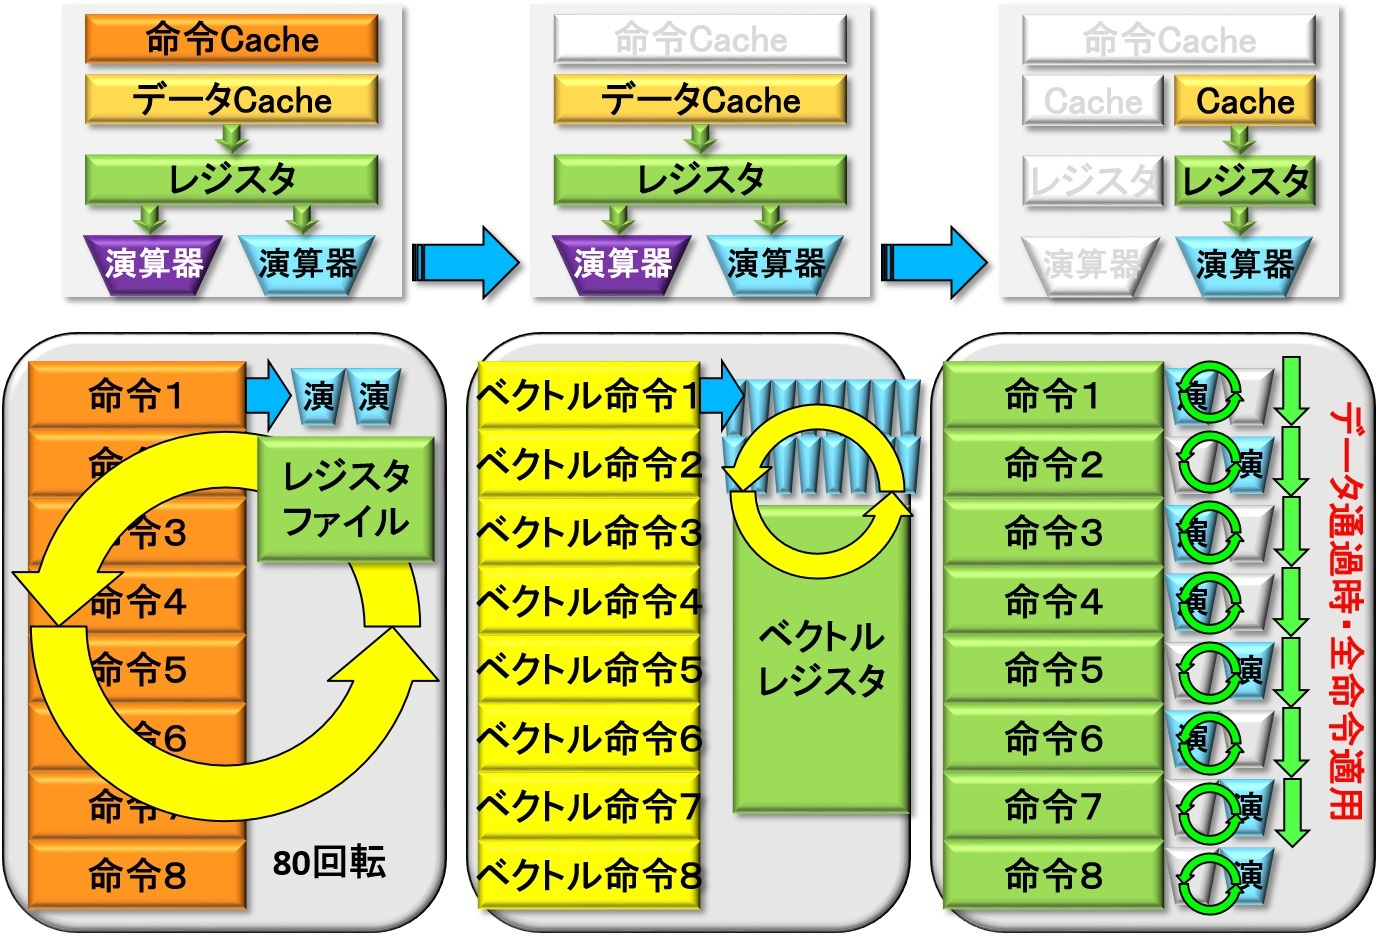
\includegraphics[angle=270,origin=b,width=0.70\textwidth]{CGRA0.eps}
\caption{\label{cgra0}CPU/GPU��CGRA��̿��¹ԥ�ǥ�ΰ㤤}
\end{figure}

\begin{figure}[htbp]
\center
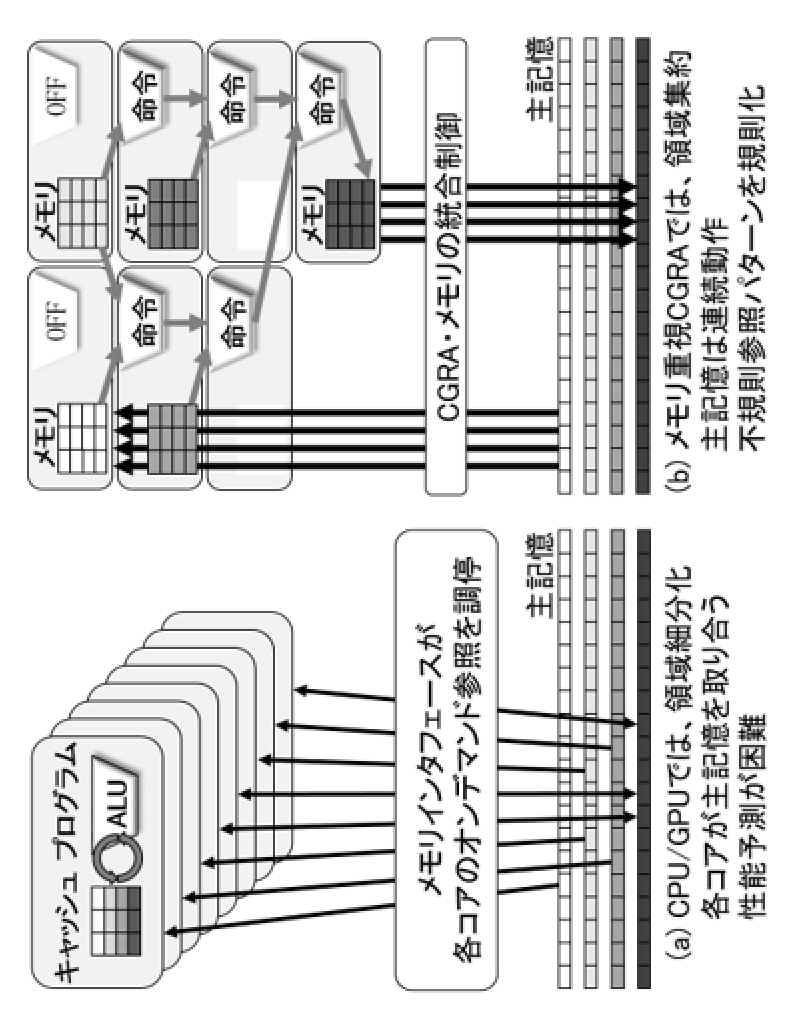
\includegraphics[angle=270,origin=b,width=0.60\textwidth]{gpu.eps}
\caption{\label{gpu}CPU/GPU��CGRA�Υ��ꥢ�������ΰ㤤}
\end{figure}

������̿�᤬�黻��ȥ�����༡���椹��Υ��ޥ󷿷׻����פϡ�ȾƳ�����ٲ���
����������ٲ���ξ�ؤ���ǽ�����٤��Ƥ��������Ԥ�ʪ���³��˶��դ���Ԥ��ɵ�
���줿��GPGPU�Ͻ��跿�ץ�����ޥӥ�ƥ���ݻ����Ĥ����������Ԥ�����ˡ���
���ϥ쥸�����ե�����ȥޥ������åǥ��󥰤ˤ��1000���������Ķ����絭����
�䱣�õ�ǽ�������롥���������絭�����Ƚ����§��������塼�˥󥰤��񤷤���
�׵���ǽã���Τ���˲���ʱ黻ǽ�Ϥ����Ϥ�ɬ�פȤ��롥������1982 ǯ��
H.T.Kung �餬�󾧤���Coarse Grain Reconfigurable Architecture(CGRA)�ϡ�����
�롼�פ�̿����򣲼������֤α黻��ͥåȥ���˼������Ƽ絭���ǡ�����ή����
����Υ��ޥ󷿤Ǥ���ʿ�\ref{cgra0},\ref{gpu}�ˡ�¿���ι����Ȥ���ꤹ���
�ץ�����ޥӥ�ƥ����ɤˤ��ű�ह���桤Google�Ҥ�TPU��Wave computing�Ҥ�DPU
��AI���Ѥ˹ʤ���Ψ�����������Ƥ��롥���漼�Ǥ�2008ǯ��VLIW�ߴ���LAPP��ȯ
�������θ塤64�ȤΥ˥�����ⵡǽ�黻���¿�ť롼�פ���������ˤ�����Ѹ�Ψ
(�黻��ǽ/����)������Ū�˹�᤿IMAX��ȯ������¿���Υ�����SIMDư�����
GPGPU�����������껲�Ȥ�Ϣ³���ɥ쥹�����礹�륳���쥷�󥰤ȹ�ڤʥ����
����ɬ�פȤ���Τ��Ф�����������¿���α黻���Ĥ�¿��Ϣ�뤹�뤳�Ȥǥ����
���η��̲��������ϲ���ã�����Ƥ��롥

\begin{figure}[htbp]
\center
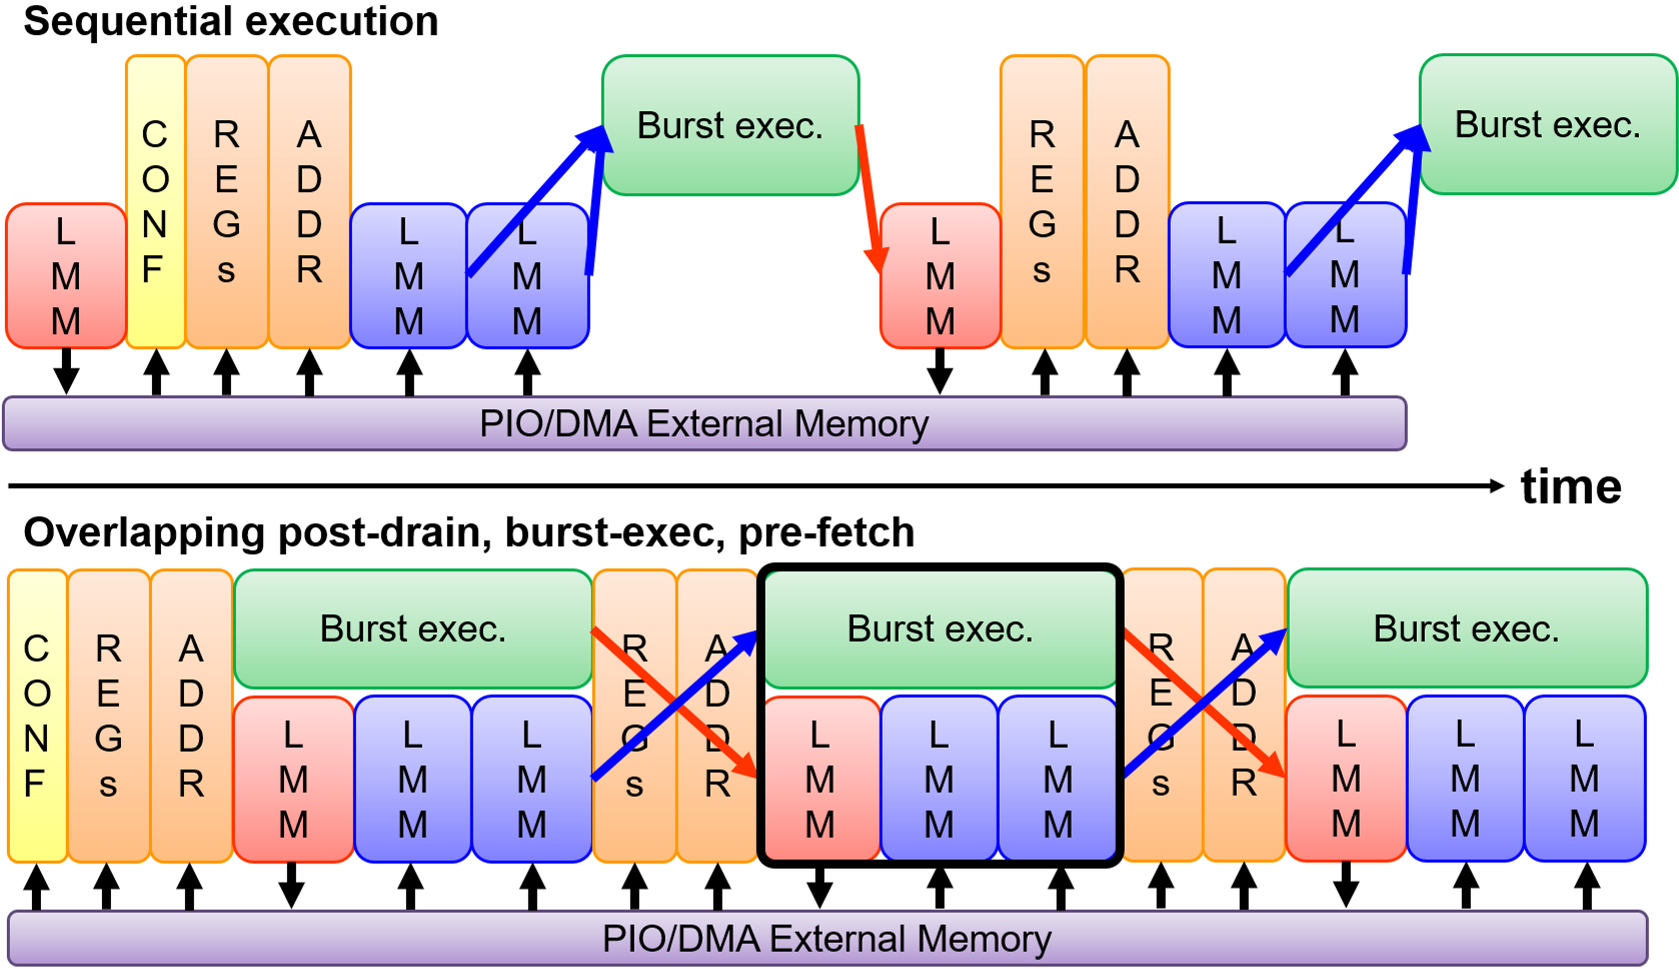
\includegraphics[angle=270,origin=b,width=0.60\textwidth]{cgra.eps}
\caption{\label{cgra}CGRA������Ūư��}
\end{figure}

\begin{figure}[htbp]
\center
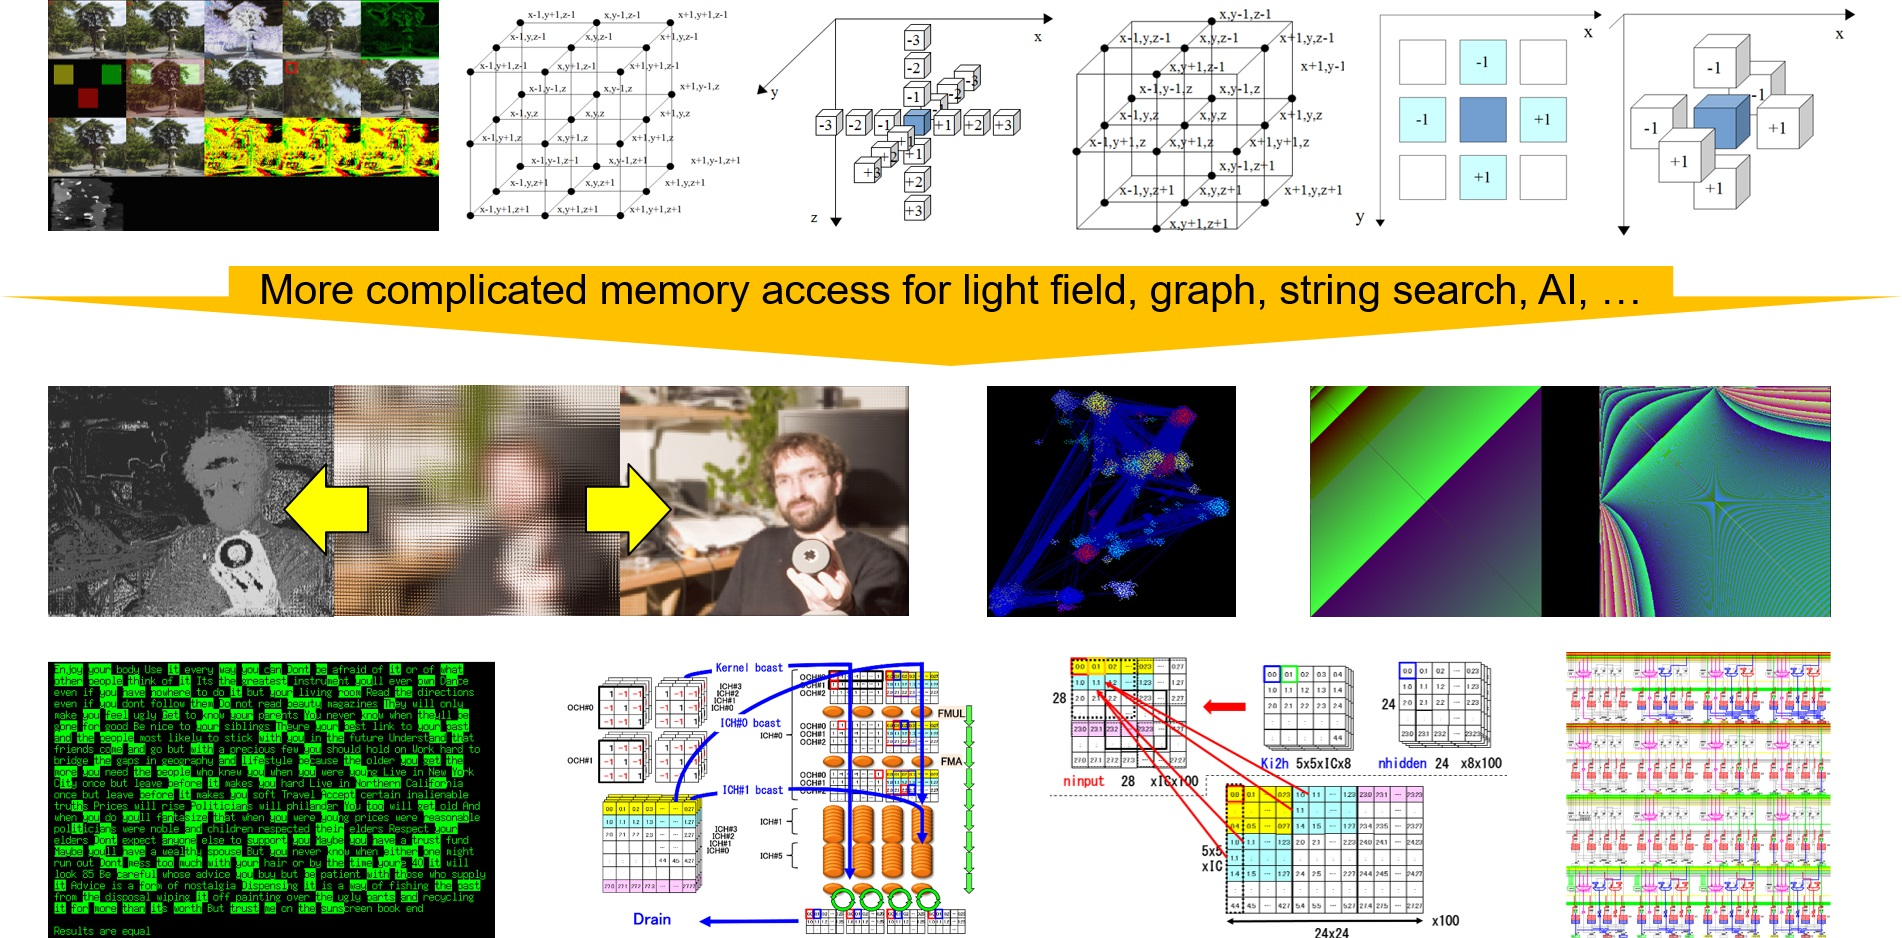
\includegraphics[angle=270,origin=b,width=0.98\textwidth]{APPL.eps}
\caption{\label{appl1}ʣ�������륢�ץꥱ�������}
\end{figure}

\begin{figure}[htbp]
\center
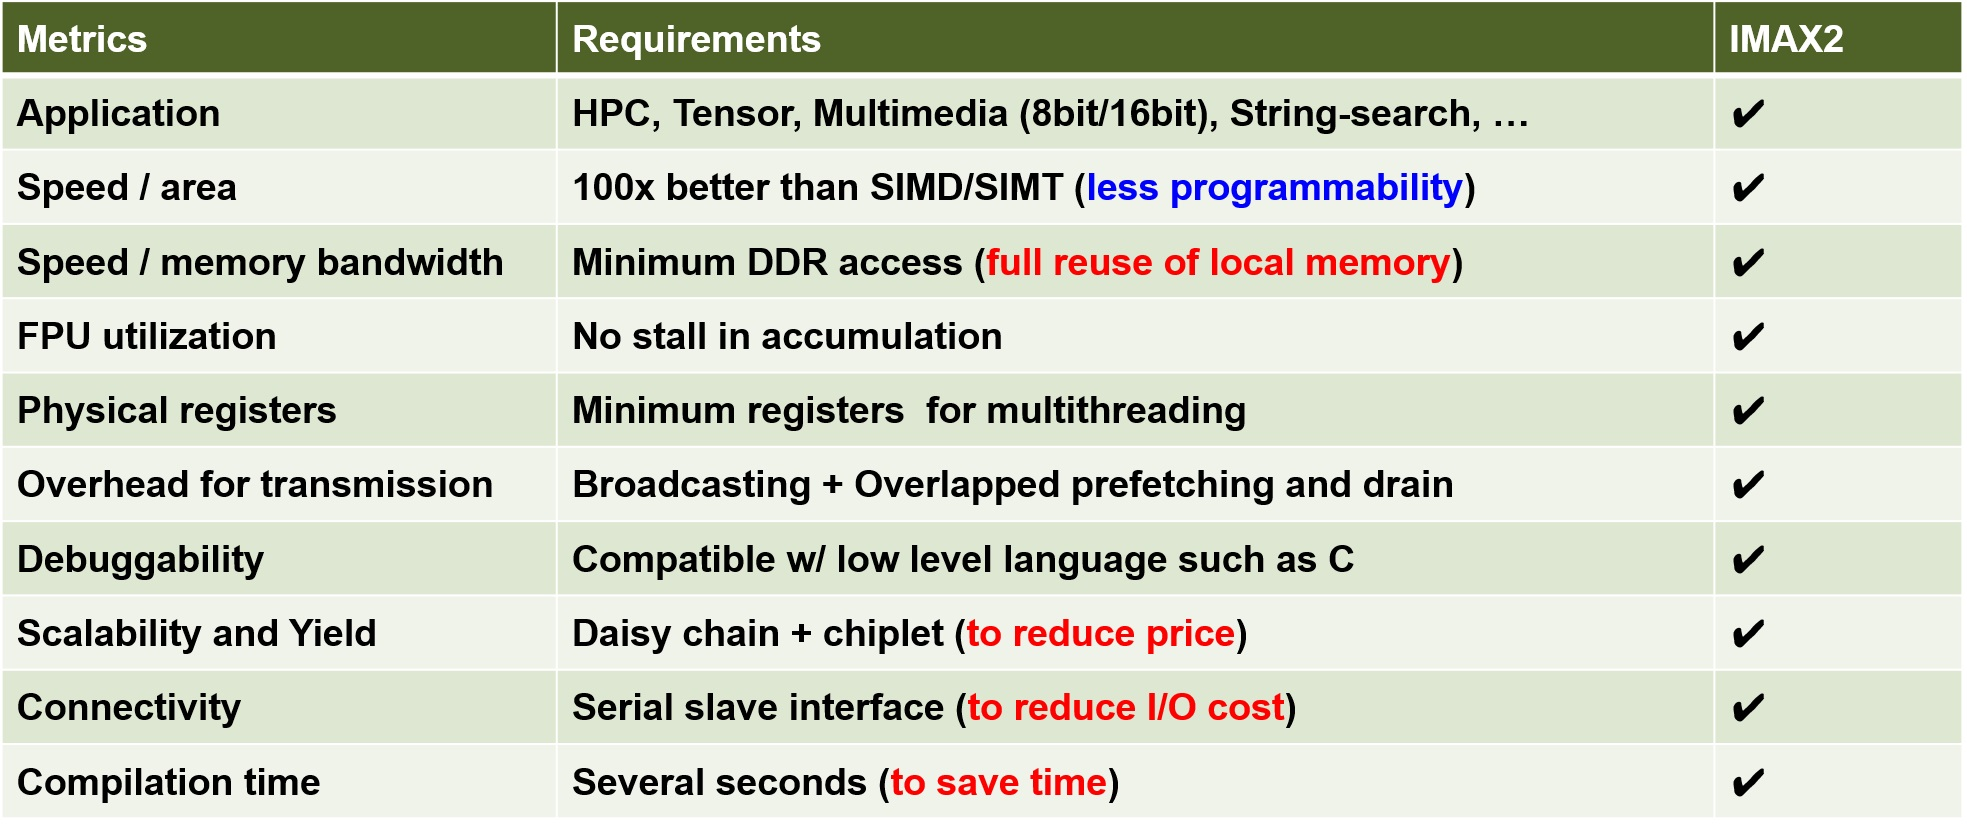
\includegraphics[angle=270,origin=b,width=0.98\textwidth]{LIST.eps}
\caption{\label{list1}����CGRA���׵ᤵ��뵡ǽ}
\end{figure}

CGRA������ʱ黻����٤˼¹Ԥ�����ȤߤǤ��뤿�ᡤ��Ψ�褯���Ѥ���ˤϡ���
\ref{cgra}�Τ褦�ˡ�ľ���α黻��̤μ絭���ؤ��ɤ��Ф����黻������ӡ����α�
����ɬ�פʥǡ����μ絭������μ����ߤ򥪡��Х�åפ������黻����Ư��³��
�뤳�Ȥ��ˤ�ƽ��פǤ��롥�ޤ�����\ref{appl1}�Τ褦�ˡ����ץꥱ�������ϵ�
®��ʣ�������Ƥ��ꡤCGRA�ˤϡ���\ref{list1}�˼���¿���ε�ǽ���׵ᤵ��Ƥ��롥

\begin{figure}[htbp]
\center
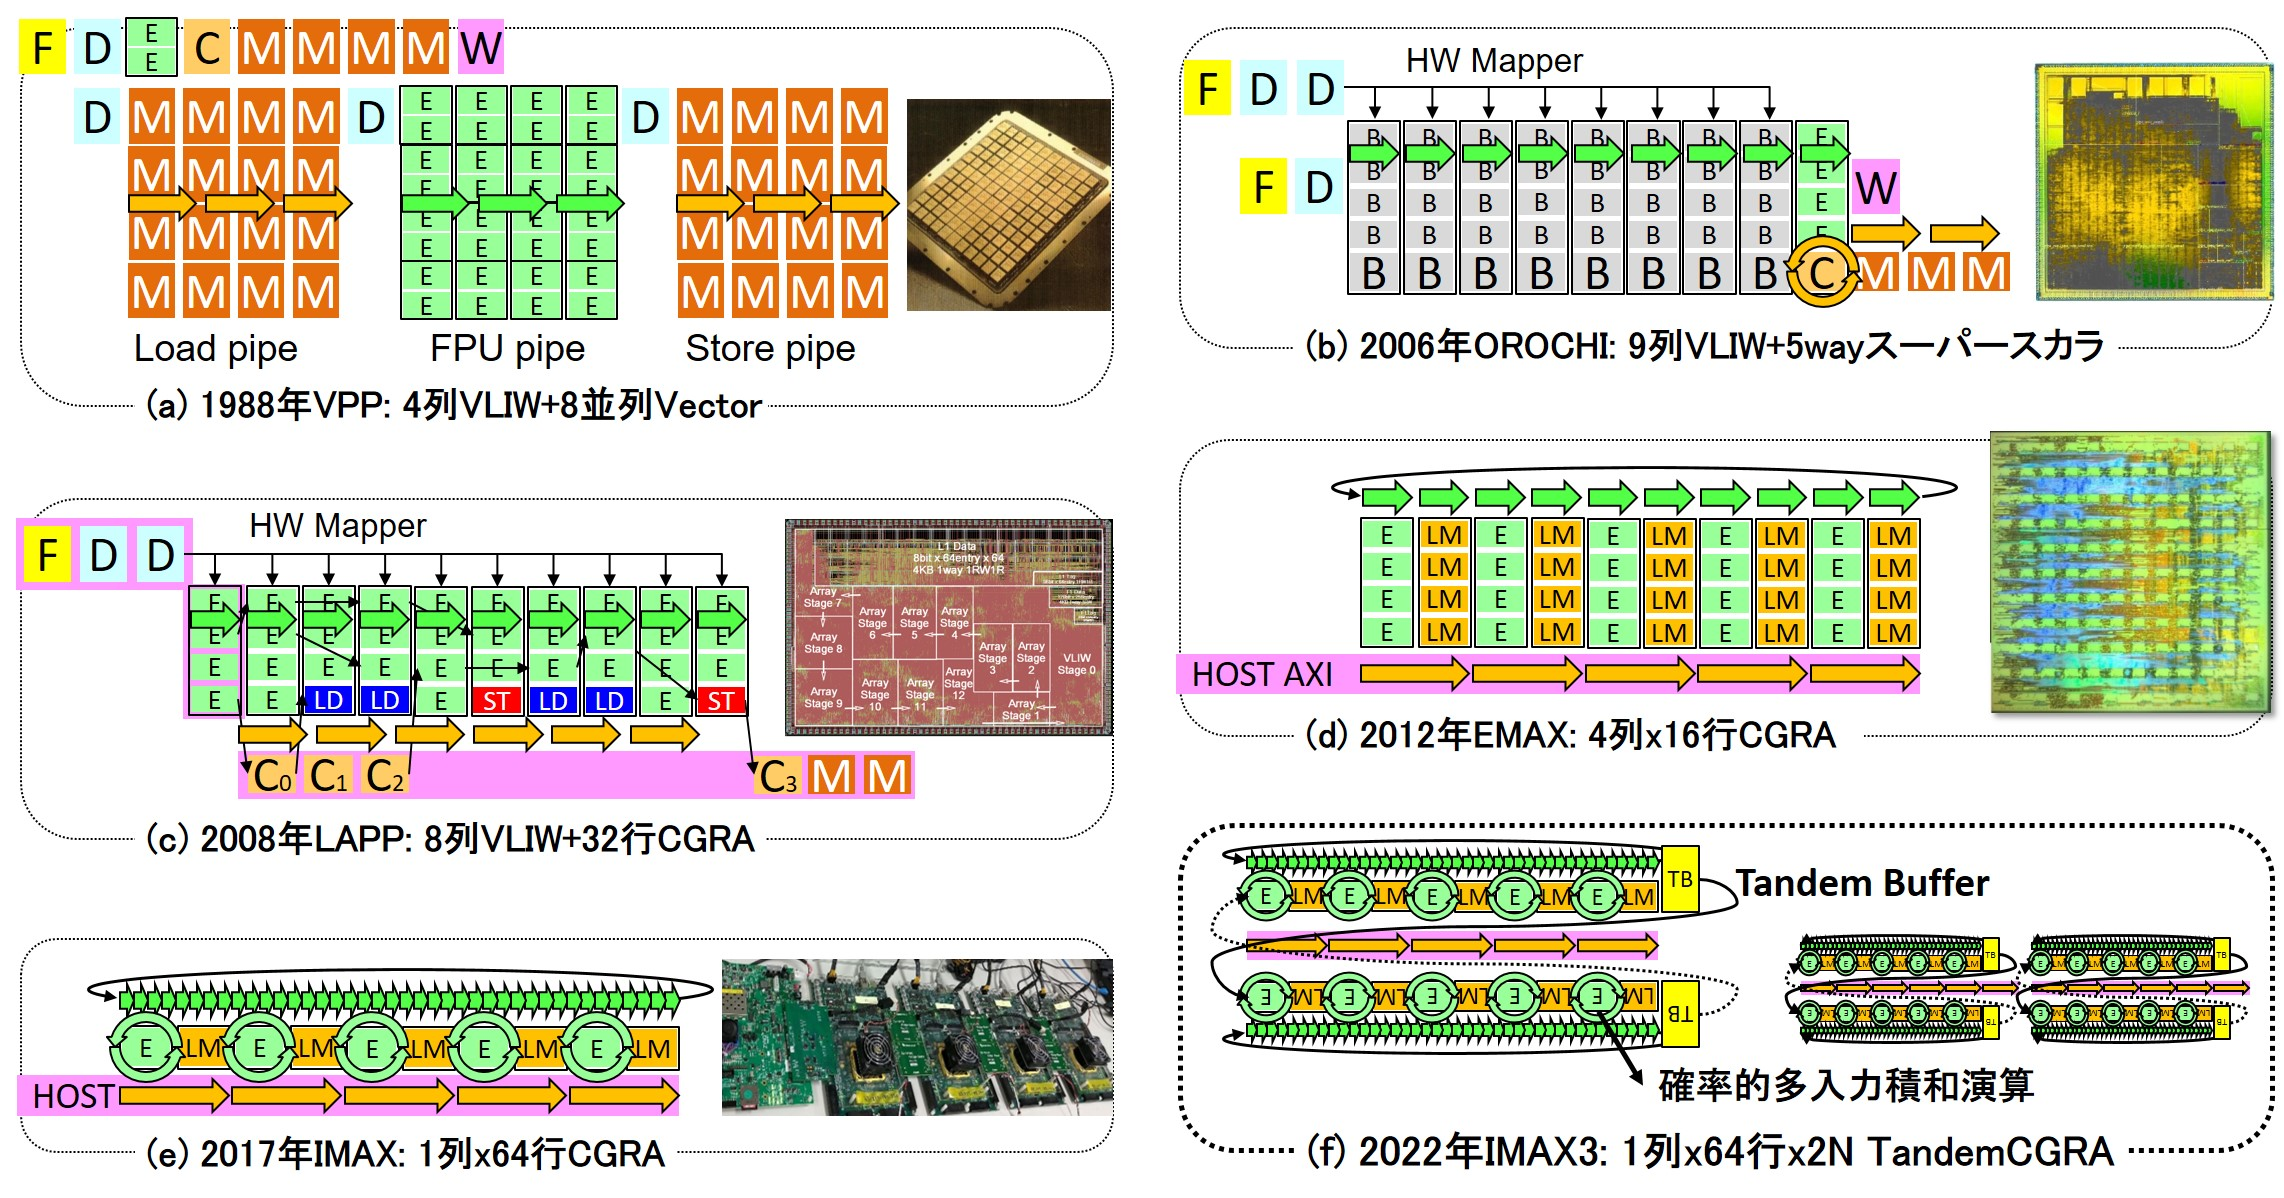
\includegraphics[angle=270,origin=b,width=0.98\textwidth]{CGRA1.eps}
\caption{\label{cgra1}VPP����IMAX�˻��̿��¹ԥ�ǥ�����}
\end{figure}

\begin{figure}[htbp]
\center
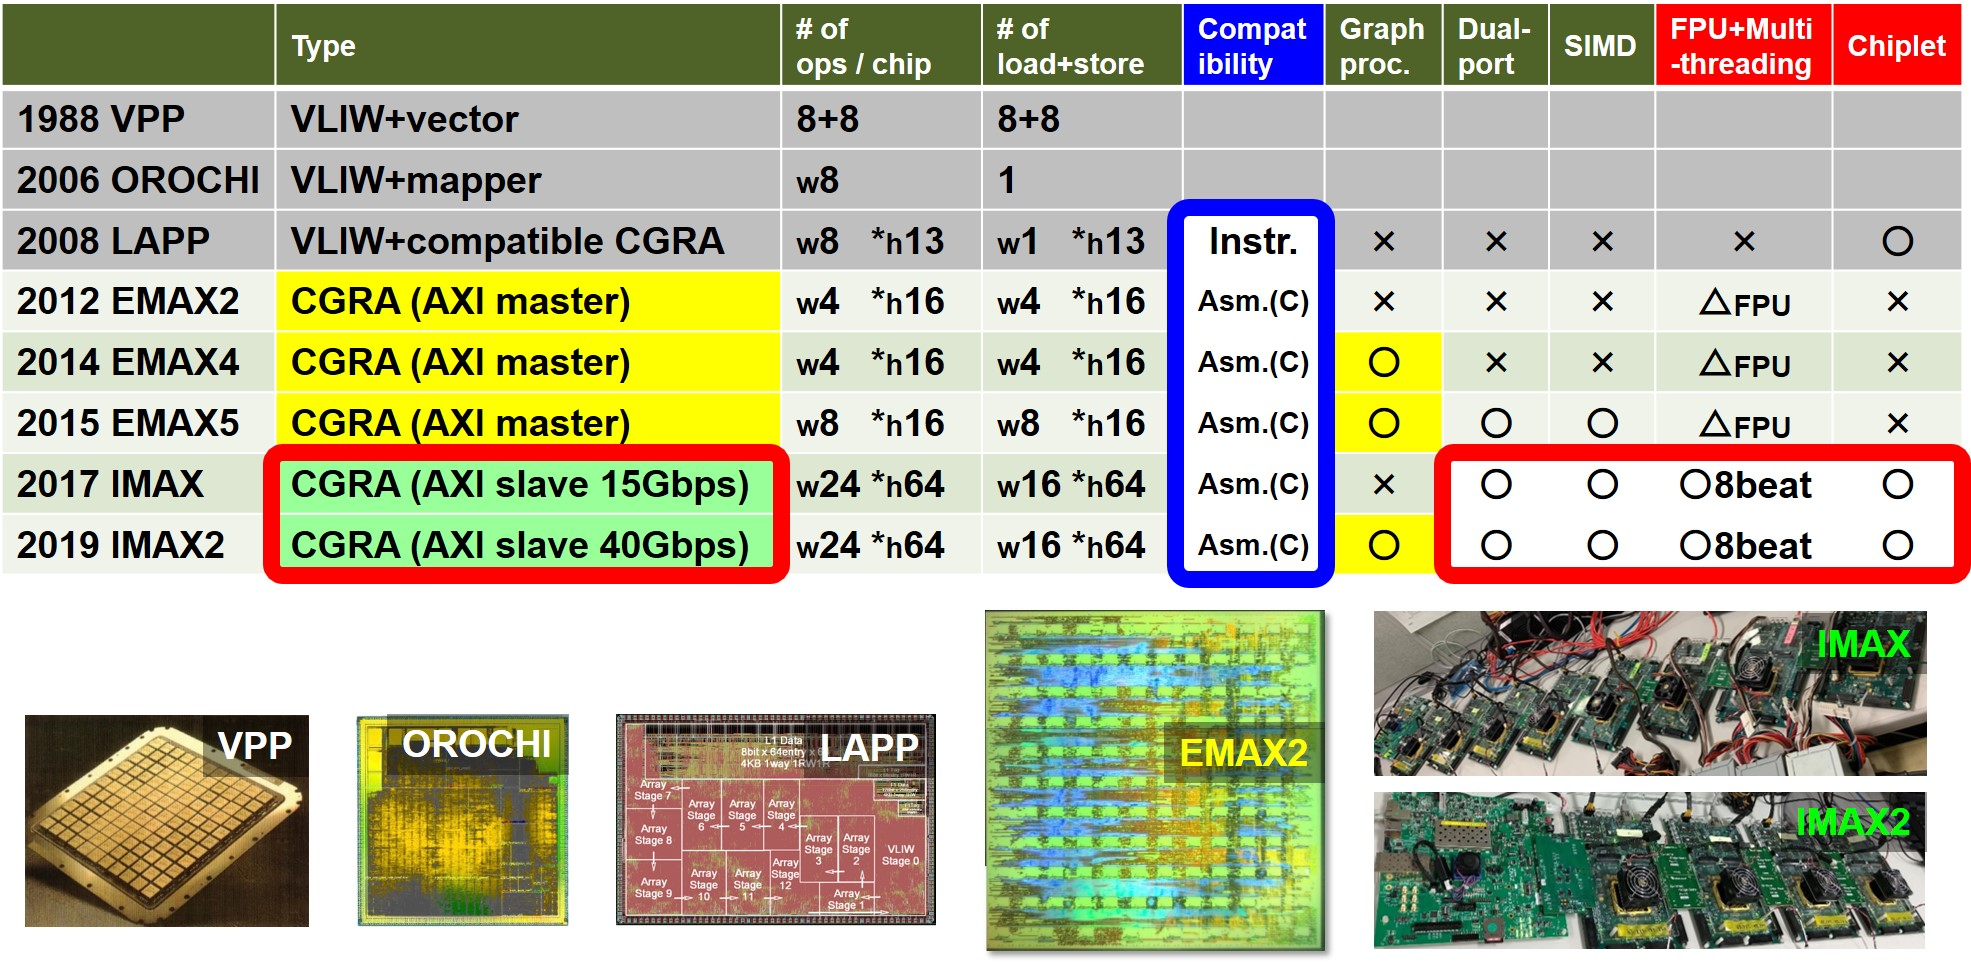
\includegraphics[angle=270,origin=b,width=0.98\textwidth]{HISTORY.eps}
\caption{\label{history1}VPP����IMAX�˻����׵�ǽ������}
\end{figure}

IMAX�˻��аޤ��\ref{cgra1},\ref{history1}�˼�����æIBM�ߴ���(a)����٥���
��VPP���꡼���Ǥϡ������᡼�����������ѡ�������˷����桤���ϸ�Ψ���粽�Τ�
��VLIW����Ƥ����Ѥ��줿��VLIW+�٥��ȥ�黻�����ϡ�����ѥ���M�ȱ黻�ѥ���
E�ΥС�����ư�CGRA�˹�������ΤΡ��ץ��������Ф��빽¤Ū���󤬤ʤ���
Ĺ��ͭ���롥(b)OROCHI�ϡ�̿��ǥ�����D��VLIW�Хåե�B��ARM̿���ưŪʬ������
��������å���C��ͭ����VLIW���ѷ������ϥ����ѡ�������Ǥ��롥VLIW��2������
ĥ���Ѥ�CGRA�������Ѥδ��äǤ��ꡤ���VLIW�ߴ�CGRA�Ǥ���(c)LAPP���Ѿ�������
(d)EMAX�ʹߤϡ��黻��E�ȥ����������LM�Υ����³�ˤ��LM��������Ѥ䡤��
��Ū����ˤ��ǡ����ե��������ӽ����ˤ�ꡤΥ�����ƥ󥷥�׻��䥰��ս�����
���Ψ����ã��������Google�Ҥ�TPU (�����黻�Τ�)��Ʊ������(e)IMAX�Ǥϡ�ʪ��1
��x64�Ԥ�����4��x64�Ԥ˲��۲�����¿�ż¹Ԥ�ͰƤ���LM�κ�������Ѥ�ʻ���ơ�
�߻�����ư���������±黻E�����Ѹ�Ψ(�黻��ǽ/����)���Ū�˲���(28nm�������
����GPGPU��250��)������(f)Tandem CGRA�ϡ����۲������ˤ��ץ�����ޥӥ�ƥ�
����夵���빽���Ǥ��롥

\clearpage

\section{History of CGRA}

\begin{figure}[htbp]
\center
\epsfile{file=CGRAHIST1.eps,width=0.98\textwidth}
\caption{\label{cgra2}LAPP����IMAX�˻��黻��ͥåȥ�����Ѳ�}
\end{figure}

��\ref{cgra2}�ˡ������롼�פ���ȯ���Ƥ���CGRA��1��ʬ�ι�¤�򼨤���LAPP��VLIW
�ߴ�CGRA�Ǥ��ä���ΤΡ�FIFO�ˤ�깽�������ƹԤΥ�����������LMM������
�Ϲ⡹16����x4��Ⱦ�������������1�դ�Ĺ���ˤ��礭�ʥ��ƥ󥷥�׻��ˤ��б���
���ʤ��ä���EMAX2�Ǥϡ�VLIW�ߴ���������������˳Ʊ黻������Ѥ�������LMM��
FIFO�����֤���¿���Υ��ƥ󥷥�׻�������Ǥ���褦�ˤ�������������LMM������
�䤷�����Ȥˤ��Դ֥쥸��������32�ܤ��������ä��������Τ��ᡤ�쥸���������
������ϤޤǤ�4����������פ�����EMAX4�Ǥϡ�����˥���ս�����ɬ�פȤʤ�ȥ�
�󥶥�����󵡹����ɲä�����EMAX2����EMAX4�ؤ��ѹ����ϰʲ����̤�Ǥ��롥

\begin{itemize}\parskip 0pc \itemsep 0pc
\item ʣ�������ȹ礻�ˤ�����ռ¹Ԥ��ɲ�
\item �ȥ�󥶥������ǽ���ɲ�
\item ���ʤȳ�������δ֤Υǡ����Х���64bit*1����32bit*4�˳�ĥ
\end{itemize}

EMAX5/L2�Ǥϡ�SIMD�黻�������ɲä���ȤȤ�ˡ�ALU��EAG�����ϥ쥸�������Ѥ�
���뤳�ȤǹԴ֥쥸��������16�ܤ�Ⱦ�������쥸��������黻����ϤޤǤ�2������
��Ȥ������ޤ�����������Х�-LMM�֥��롼�ץåȤ���夵������EMAX5/ZYNQ�Ǥϡ�
FIFO����������Хإåɤ�︺���뤿���FIFO������������ˡ���������Х�
����ʣ�����LMM��Ʊ���˽񤭹���ѥ����ɲä���������ˤ�ꡤʣ���γ�������
�Х�����Ѥ���¿����LMM��Ʊ���˽�������뤳�Ȥ���ǽ�Ȥʤä���EMAX4����
EMAX5/ZYNQ�ؤ��ѹ����ϰʲ����̤�Ǥ��롥

\begin{itemize}\parskip 0pc \itemsep 0pc
\item ñ������ư�������黻��32bit*2�黻��SIMD��
\item 32bit�����黻��32bit*2�����黻��SIMD��
\item 8/16bit��ǥ����黻��4/2����SIMD����8/4����SIMD������
\item ��UNIT�Υ�����������LMM�˥Х�����32bit*1����64bit*4�˳�ĥ����
LMM-��������֤Υ��롼�ץåȤ�8�ܤ˳�ĥ
\item ���ʤȳ����������³��32bit*4*1����ͥ뤫��64bit*4*4����ͥ�˳�ĥ����
����-��������֤Υ��롼�ץåȤ�8�ܤ˳�ĥ��conf/regv/lmmi����������Хإå�
��1/8�˺︺��
\item ��������ľ�ܻ��ȤΤ����Dual-Port-LMM�κ��Ѥ����CGRA���ܹ������ѹ�
\item ����3UNIT��LMM����3����SIMD�إǡ������뤷�Ĥ�LMM�˽��ϤǤ���UNIT�֥Х��ͥåȥ��
\item UNIT����������¥쥸��������8����4�˺︺������������¥쥸������
��黻��ؤϥ������Х����å�������
\item LMM�ν��Ϥ��ʿ���������¤���FIFO������������˳�������Х�����
Ʊ���ʤ�LMM�إ֥����ɥ��㥹�Ȥ��뵡����������FIFO�ν���������ס�
\end{itemize}

IMAX�Ǥϡ�CGRA�ΰ���Ū�ʷ����Ǥ���������¿��������ӡ����ʥ롼�ױ黻���α黻
��ϩ����Ψ���㤵��������뤿��ˡ���ʿ�����α黻�ˤϸߤ��˰�¸�ط����ʤ�����
�����Ѥ���ʣ����α黻��ǽ��1���«�ͤ�ޥ������åǥ��󥰤�Ƴ������������
Ū�ˤ�ʣ����α黻��ǽ������UNIT�ˤ�¸����Ĥġ�ʪ��Ū�ˤ�1��α黻�ﷲ�ˤ�
��������뤳�Ȥˤ�ꡤ�黻����������̺︺���黻����Ѹ�Ψ���塤��ʿ�����֥���
�ɥ��㥹�Ȥ����ײ���LMM��Ĺ���Ѥ����ײ�����ǽ�Ȥʤä����ޤ���CPU�ؤ���³��ˡ
��AXI-SLAVE���ѹ�����LMM�ؤν񤭹��ߤϡ�UNIT����ߤ���vAddr-range�˽�������
UNIT����ΧŪ�˼�������ˡ���ѹ�����������ˤ�ꡤ��ľ�����֥����ɥ��㥹�Ȥ�
��ǽ�ˤʤä�������ˡ�UNIT�ν��Ϥ����Ϥ��᤹�ѥ����ɲä��뤳�Ȥˤ�ꡤƱ��
LMM���Ф���read-modify-write���ǽ�Ȥ������߹��߱黻��չ���׻���ɬ�פȤʤ�
LMM�������졼�Ȥμ������ǽ�Ȥ������ʤ���ʣ���Ԥ�LMM���Ф���Ϣ³����
vAddr-range�����ꤷ�Ƥ�����ʣ����LMM���Ф���Ʊ�쥹�ȥ���Ԥ����Ȥˤ�ꡤ������
��졼�ȶ��֤���ܤ����䤹���Ȥ��ǽ�Ȥʤä���EMAX5/ZYNQ����IMAX�ؤ��ѹ�����
�ʲ����̤�Ǥ��롥

\begin{itemize}\parskip 0pc \itemsep 0pc
\item EMAX5/ZYNQ�ȤΥץ������ߴ�����ݻ����ʤ���ʪ���黻��������LMM����
�︺
\item AXI-SLAVE����lmring��8��8����������ӡ���ľ�����֥����ɥ��㥹�ȵ�ǽ
�ˤ��ۥ��ȼ絭����LMMž����Ψ�θ���
\item Ʊ��LMM����Ѥ���read-modify-write��ǽ�ȥ������졼�ȵ�ǽ
\item Ʊ��LMM����֥�Хåե��Ȥ��ƻ��Ѥ��륿��ǥൡǽ (FFT��¿�ʥޡ��������Ȥ�����)
\item �ǥ奢��ݡ���LMM�����Ѥ��������ɷ����Ӥ���ӥ��ɥ쥹������ǽ (¿�ʥޡ��������Ȥ��¹����Ѥ�����)
\item ���Ǥ˰��־�����ղä��ư��̤����¹���ɤ����ι����ѱ黻��ǽ
\item �ޥ�����å��б�����ӥޥ�����åפؤμ�����ޤ᤿¿�ť롼�װ��¹Ե�ǽ
\item �С�����Ĺ������8(256bit���ξ��)�Ǥ���AXI3��DMA-READ��®���Τ����ʣ
���ȥ�󥶥������ñ�첽(AXI4��)����ӥХåե���󥰵�ǽ
\item �ǥ奢��EAG�����Ѥ�����8�Х��ȶ��������64bit������
\item SIMD�����ưפˤ��롤32bit/8bit�����ɥǡ�����64bit�쥸������ĥ
\item ưŪDMAϢ��ˤ�롤ʣ��LMM���Ф���Ϣ³�ǡ���ž��
\end{itemize}

\section{Policy of IMAX}

CGRA�β���ϡ��ʣ����󼡸��ʻҹ�¤�Τޤ޼��������Ĺ��Υ����������������ư��
���ȿ���������Ѹ�Ψ���㲼��⤿�餹��������Ѳ���������ɬ�פǤ��뤳�ȡ��ʣ���
��ư�������������졼�ȱ黻��������������Ф���read-modify-write�Τ褦
���ܼ�Ū��ʣ������������פ���̿�᤬���äƤ�ѥ��ץ饤��¹Ԥ�˸���ʤ����Ȥ�
��ɬ�פǤ��뤳�ȡ��ʣ��˺���롼�פι�®�������Ǥϥ٥��ȥ�Ĺ��û�������Ѥ��
�߹��߱黻�ι�®���˸����ʤ����ᡤ��ư�����Хإåɺ︺�Τ����¿�ť롼�װ��
�¹Ե�ǽ��ɬ�פǤ��뤳�ȡ��ʣ��˥����������κ����Ѹ�Ψ��夲�Ƴ�������
���Ȥ�︺���뤿��ˡ���Ū���Ϥ�����ʥǡ������ȥѥ��������ư���ɿ�Ǥ���̿
��������֥��եȵ�ǽ��ɬ�פǤ��뤳�ȡ��ʣ��˹ⵡǽ��DMA�ޥ�����ǽ����¢��ɬ
�פȤ������Ǥ�DMA���졼�֥���Ȥ��ƹ��Ψ��ã���Ǥ��뤳�ȡ��ʣ��˳������
��Х���AXI�ˤ����ߤ�ɬ�פȤ��������졼�֥���ε�ǽ�������������������ǥ�
�󥰤ˤ�ꥹ������֥����ǽ���ưפ������뤳�ȤǤ��롥

IMAX���裱�Υݥ���Ȥϡ�CGRA��̾�Τˤ����̤��Τ��Ƥ��룲���������Ȥ��礭
���ۤʤꡤ�㥳���Ȥ��׵ᤵ���IoT���å�������ʪ����¤�򣱼����ʥ�˥����쥤��
�Ȥ��ĤĹ���ǽ��ݻ��������Ǥ��롥�裲�Υݥ���Ȥϡ����굡ǽ��������ͻ�礷��
�ۥ��Ȥ������Ȥ��ƻ��Ѥ��뤿�ᡤ�̾�Υ�������졼���������ž��������
�إåɤ˶줷��Τ��Ф���ͥ�̤���������ӡ�����Ǥ��뤳�Ȥ����Ѥ�����������
����³���ưפ����Ǥ��롥�裳�Υݥ���Ȥϡ����굡ǽ�ȱ黻��ǽ�����Ū�˼��
����ľ��Ū�ץ�����ߥ󥰤Τ�����͡��ʥǡ����ѥ����������äˡ��̾��CGRA����
���դȤ��롤Ʊ��������������Ф���read-modify-write��¿�ť롼�������
��ץ�ʹ�¤�ˤ���ǽ�Ȥ������Ǥ��롥�裴�Υݥ���Ȥϡ��ǡ����ѥ��ι��פˤ�
�ꡤFPGA�Τ褦��õ��Ū����ѥ����ɬ�פȤ���������ѥ���®�٤���®�����Ǥ��롥

\begin{figure}[htbp]
\center
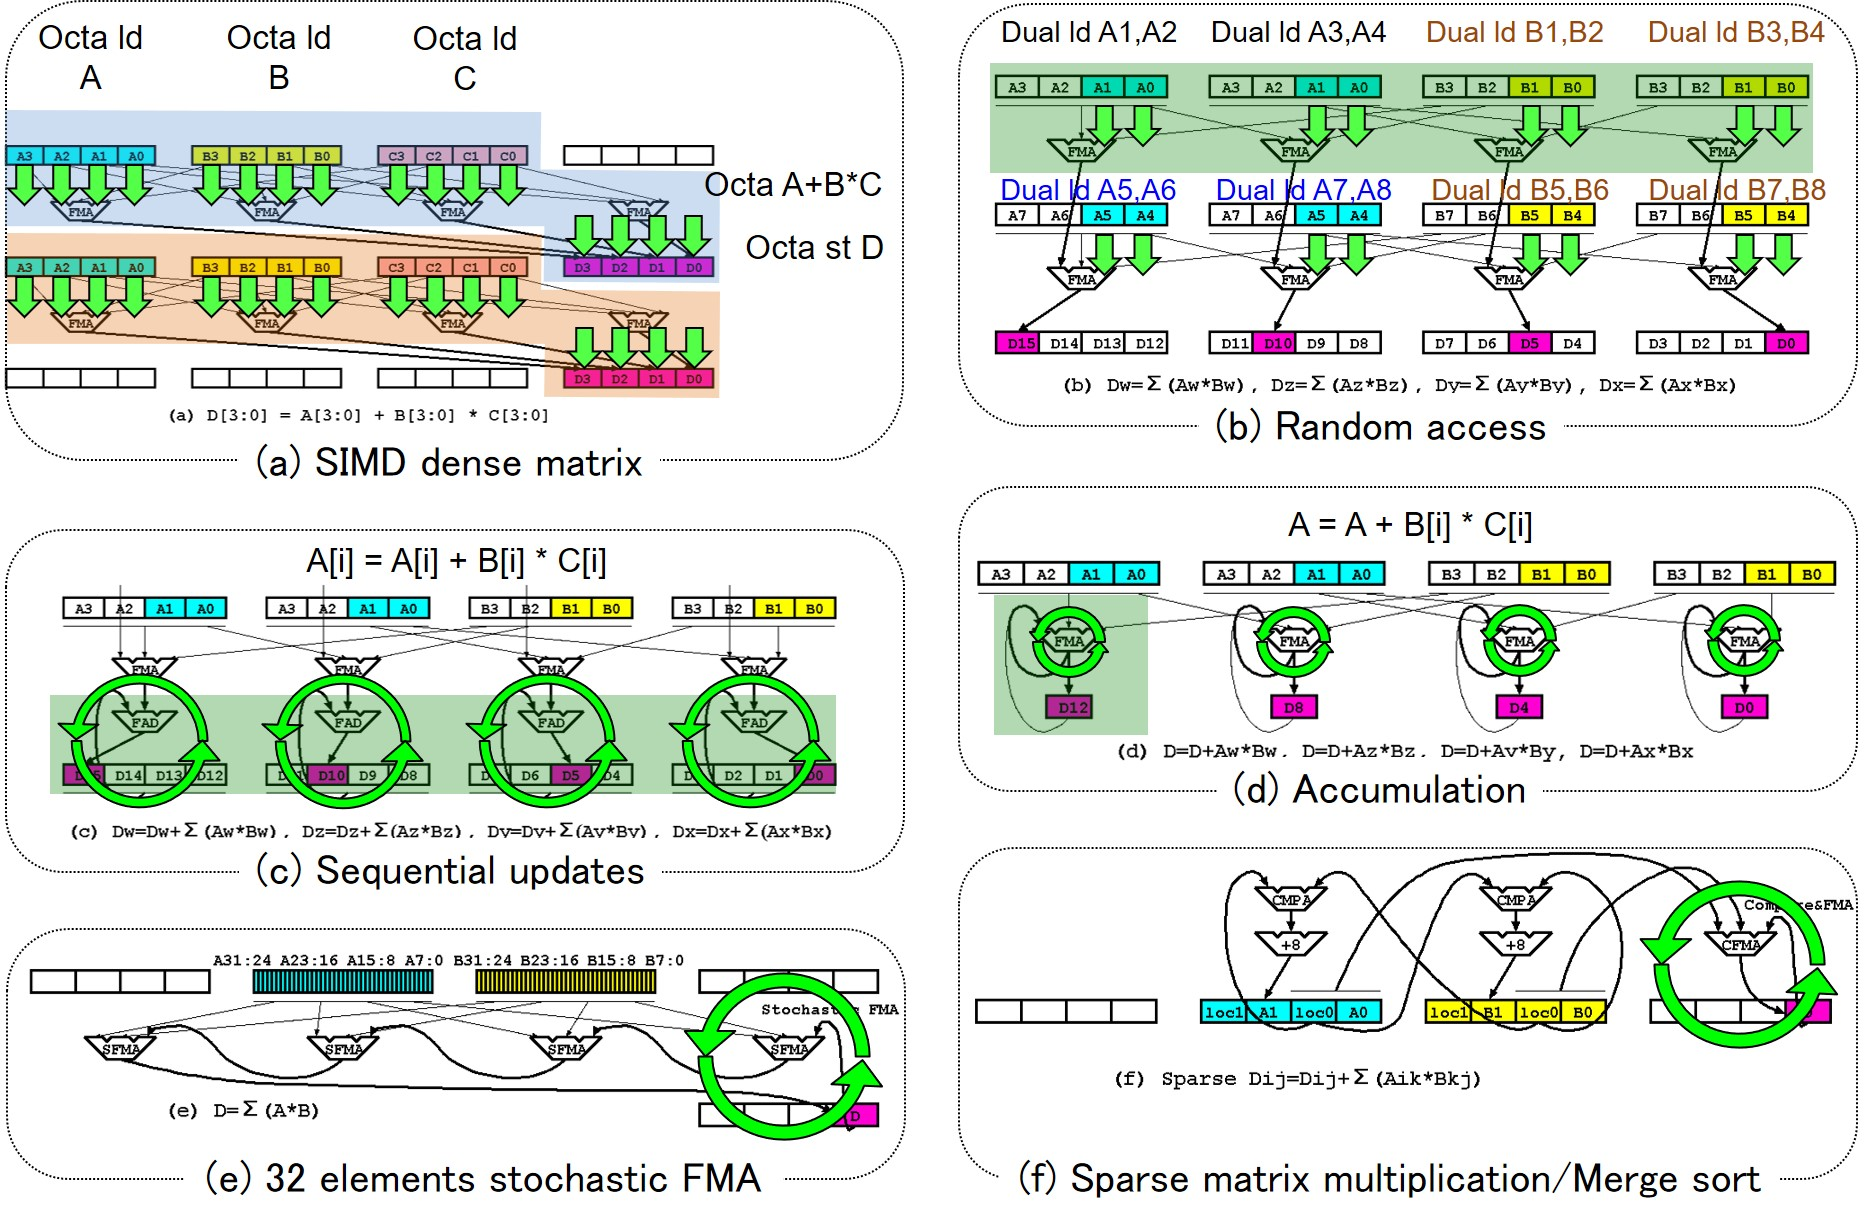
\includegraphics[angle=270,origin=b,width=0.98\textwidth]{EMAX6EXP.eps}
\caption{\label{exp}ɬ�פȤ������껲�ȥѥ�����ȱ黻}
\end{figure}

IMAX�ˤϡ�1��x64�Ԥ�ʪ����¤���Ф��ƺ���10̿���2�黻x3stage + ������x2 + ��
�ȥ�x2��x4��x64�ԡ�2560̿�����٤˼����Ǥ��롥IMAX�ϴ���unit��1��x64��(���)
���֤���ʪ����¤��ͭ�����ΤΡ��ץ�����ߥ󥰻��Υϡ��ɥ�������ǥ�ϡ�4��
x64�ԤǤ��롥��unit��3�ʥѥ��ץ饤���3����ñ������ư�������ø��軻���2����
����64�ӥå����Υ쥸��������Ѥ��ƣ��Ĥα黻��Ʊ���¹Ԥ��롥�ޤ����ѥ��ץ饤
��ν��ʤ�8/16/32�ӥå�ñ�̤γƼ�ޥ����ǥ����黻����Ӹ��꾮�����黻����
�ʤ������黻�����ʤϥ��եȱ黻����Ԥ����Ȥ��Ǥ��롥��unit��64KB�ǥ奢��ݡ�
�ȥ���������Ƥ��ꡤ��\ref{exp}�˼����͡��ʥ��껲�ȥѥ�������б��Ǥ��롥
(a)�ϡ�1�ԤΥ�����������LMM�ˤ˳�Ǽ���줿A,B,C��4��ɤ����ɤ߽Ф���4��
�α黻��ˤ��SIMD�黻��Ԥä��塤�黻���D���ʤ�LMM�˳�Ǽ�����Ȥ�2���å�
�����������֤Ǥ��롥A,B,C�ϳ������꤫�鶡�뤵�졤D�ϳ�������˼��Ф���
�롥(b)�ϡ��������˾��߹��߱黻��Ԥ������Ǥ��롥�ǥ奢��ݡ��ȥ��꤫���
��α黻���A��B�򶡵뤷��4�����ξ��߹��߱黻��ԤäƤ��롥(c)�ϡ�LMM��4����
��D���߻���������Ǥ��롥����Ū��CGRA�Ȥϰۤʤꡤ���ΤȤ��Ƥϥǡ�����ή��
���¤��Ĥġ��߻���Ԥ����Ȥ�Ǥ��롥(d)�ϡ�Ʊ�ͤ�LMM��4������D���߻��������
�Ǥ��롥����������Ǽ�褬���ꤵ�졤LMM�ؤ�read-modify-write�ˤ�ꡤ���٤⹹��
��Ԥ������б����롥(e)��UNIT��¿�������±黻�����γ�ĥ��ǽ�Ǥ��롥(f)����
����ι����Ѥ�ޡ��������ȤǤ��롥

\begin{figure}[htbp]
\center
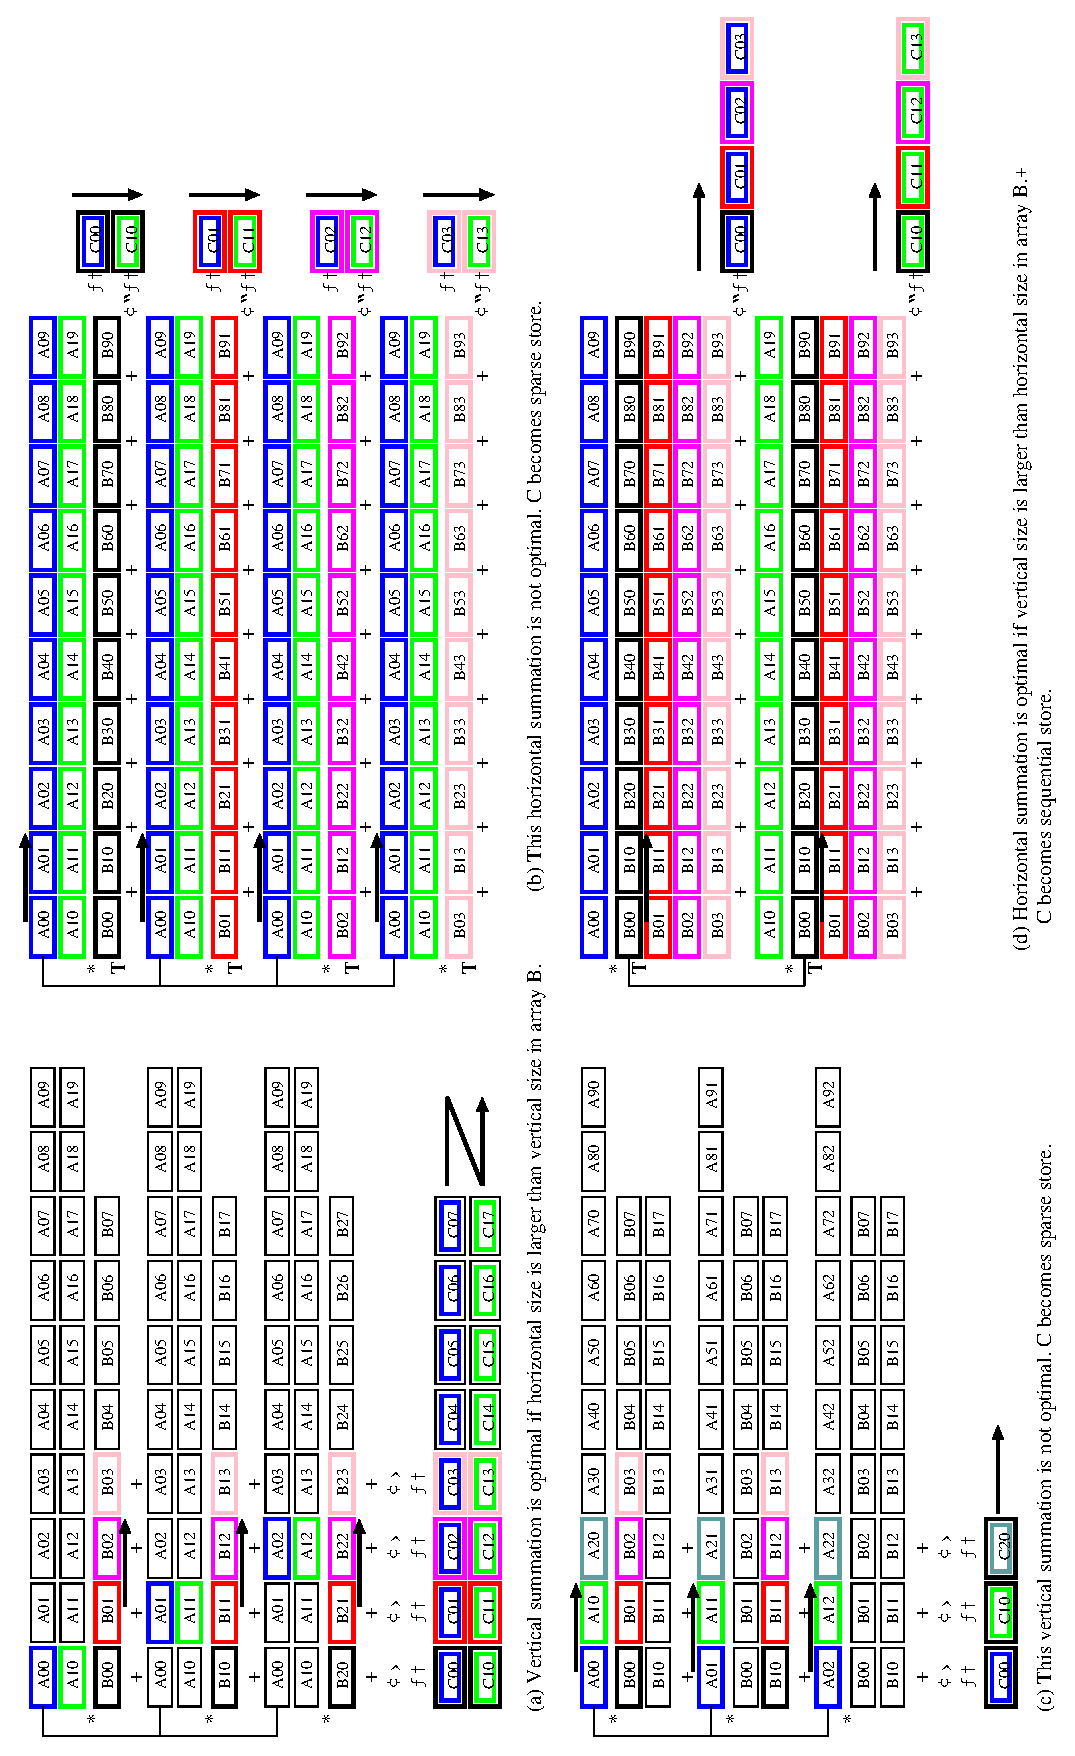
\includegraphics[angle=270,origin=b,width=0.98\textwidth]{CGRAPAT.eps}
\caption{\label{fig:cgrapat}�����Ѥα黻����}
\end{figure}

�㤨�й����Ѥξ�硤��\ref{fig:cgrapat}�˼����褦�ˡ���Ŭ���߻�����������B��
�����ˤ�äưۤʤ롥�߻���������(a)�ξ�硤��\ref{exp}(b)����ӿ�
\ref{exp}(c)��ɬ�פȤʤ롥�߻�����������(b)������C�ؤΥ��ȥ�����Ϣ³�Ȥʤ뤿
���Ŭ�ǤϤʤ���Ʊ�ͤˡ��߻��������Ĥ�(c)������C�ؤΥ��ȥ�����Ϣ³�Ȥʤ뤿��
��Ŭ�ǤϤʤ���ʣ���Ԥ�B��«�ͤ�(d)�ξ�硤��\ref{exp}(d)�ޤ��Ͽ�\ref{exp}(e)
��ɬ�פȤʤ롥����Ƹ���ȡ�(a)�Ǥ�����Aʣ���Ԥο�ľ�����֥����ɥ��㥹�ȡ�
(d)�Ǥ�ž�ָ������Bʣ���Ԥο�ľ�����֥����ɥ��㥹�Ȥ�ɬ�פȤ��������ۤʤ��
�ΤΡ�����C�ؤΥ��ȥ���Ϣ³�ΰ�Ȥʤ롥

\section{�����Ѳ��Τ�����������ޥ������åǥ���}

\begin{figure}[htbp]
\center

\includegraphics[angle=0,origin=b,width=0.98\textwidth]{unit.eps}
\caption{\label{fig:unit}Column multithreading for small footprint and
bubble-free execution}
\end{figure}

����ʣ��ˤȡʣ��ˤ��б����뤿��ˡ��������ޥ������åǥ��󥰤�Ƴ����������
\ref{fig:unit}(a)�ˡ�Ƴ�����ΰ���Ū��unit�����򼨤������̤�CGRA�ϡ�����α�
���Ȥ�Ʊ�������Ȥ�︺���뤿�ᡤ�Ʊ黻�郎�襵������黻��̤���Ϥ��������
�߷פ���롥���Τ��ᡤ��ư�������������졼�Ȥʤɱ黻���֤�Ĺ����ǽ��ѥ���
�饤�󲽤��뤳�Ȥ��Ǥ������Ѹ�Ψ���������롥�ޤ���LMM����¿�����ɤ߽Ф����
������ˡ�Ʊ�����Ƥ��ݻ�����ʣ����LMM�����֤���¿�ݡ��Ȳ�����ɬ�פ����ꡤ��
�Ѹ�Ψ�������װ��Ȥʤ롥��\ref{fig:unit}(b)�ϡ��ޥ������åǥ��󥰡�W=4��Ŭ
�Ѹ��unit�����Ǥ��롥1�Ĥ�unit��4�����������Ѥ�������Ū��(a)��Ʊ����ǽ��
�¸����롥Reg\#0-15�����򤹤�16-to-1���쥯����ޤ�Ʊ黻���4�ʥѥ��ץ饤��
������ʿ����4�Ĥα黻���ʬ��¹Ԥ���ȡ���ư�������������졼�Ȥ�¸�ߤ���
��Ʊ����ǽ��ݻ��Ǥ������Ѹ�Ψ��4�ܤ˲����Ǥ��롥��������(a)�Ǥ�1�Ĥ�unit��
������黻�ٱ���֤�2��������Ǥ���Τ��Ф���(b)�Ǥ�8��������Ǥ��롥�ޤ���4
�������뤫���ƽФ���������unit�α黻��̤�LMM�ɤ߽Ф��ǡ��������Ƥ���unit
�����Ȥ��뤿��ˡ�Reg\#0-15�Υ��֥�Хåե���󥰤�ɬ�פȤʤ��grp.A�����
grp.B�ˡ�LMM�˴ؤ��Ƥϡ�2�ݡ���LMM��4��������ư��ˤ��8�ݡ��Ȳ�����ȡ���ʿ
����4�Ĥ�LMM�����ƽ�ʣ�������硤���Ѹ�Ψ��4�ܤ˲����Ǥ��롥��ʣ���ʤ����
��LMM�����̤�ʬ����Ѥ��뤿��������Τθ�Ψ���Ѥ��ʤ���ΤΡ����ɥ쥹��
����Ϻ︺�Ǥ��롥AXI-WRITE-IF�����AXI-READ-IF�ϡ��黻�ѥǡ����ѥ���LMM��
load/store�ݡ��Ȥ�Ȥ�ʤ�������������Ѥ���LMM�򻲾Ȥ��롥

\begin{figure}[htbp]
\center
\epsfile{file=CGRAHIST2.eps,width=0.98\textwidth}
\caption{\label{cgra3}IMAX�ˤ�����쥸�������֥�Хåե���󥰤ν�����}
\end{figure}

��\ref{cgra3}�ˡ�IMAX�ˤ�������֥�Хåե��ν������򼨤���(a)��4�����ΰ�
��Ū��CGRA�ˤ��������ȱ黻��δط��Ǥ��롥�����3�ս꤫��ơ�4��ɤ�
�ɤ߽Ф�������ư���4�黻��ν���(4���ʬ)�����˽񤭹��ि��ˡ�
3-read 1-write���꤬ɬ�פǤ��롥4�ʥѥ��ץ饤��������ư�������黻��ξ�
�硤���ɥ쥹�֤˰�¸�ط����ʤ���Х��롼�ץåȤ��㲼���ʤ���ΤΡ��߻��Τ褦
�˰�¸�ط�������ȡ����Ϥ����Ȥα黻��̤��Ԥ���碌�뤿��ѥ��ץ饤�����
������ǽ��1/4���㲼���롥�ѥ��ץ饤���ߤ�ʤ�����ˤϡ�(b)�Τ褦��1�黻��
�Τߤ��Ѥ���4way-�ޥ������åǥ��󥰲�����Ф褤�����������黻��Ϻ︺�Ǥ�
�Ƥ⡤����Υݡ��ȿ��Ϻ︺�Ǥ��ʤ���(c)�ϥݡ��ȿ��︺�Τ����SIMD-LD������
�����������Ǥ��롥�ץ�������SIMD-LD, SIMD-FMA, SIMD-ST���ȤȤ��Ƶ��Ҥ��롥
�ϡ��ɥ������ϡ�4��������Τ���3�����������Ѥ���3�ս꤫��SIMD-LD�ˤ���ɤ�
�Ф���Ԥ�����ö�����֥�Хåե�����¸���뤳�Ȥǡ�4������������Ƥˤ����Ƴ�
�黻��ɬ�פ�3���Ϥ�������Ȳ�ǽ�Ȥʤ롥�ޥ������åǥ��󥰤ˤ��SIMD-FMA��
��ʬ��¹Ԥ��졤�黻��̤���˥���˳�Ǽ����롥���ʤ����SIMD-FMA��
SIMD-ST�ϼºݤˤ�SIMDư��ʤ���ΤΡ��ϡ��ɥ���������ǽ��100\%ȯ���Ǥ��롥

\begin{figure}[htbp]
\center

\includegraphics[angle=0,origin=b,width=0.60\textwidth]{rmw.eps}
\caption{\label{fig:rmw}Read-modify-write operation}
\end{figure}

��\ref{fig:rmw}��read-modify-write operation��unit���б��򼨤�������Ū��4��
ʬ��read-modify-write��ʪ��Ū�ˤ�ñ��unit�˼�������롥���ʤα黻��ˤ����
����̡�sum0-3�ˤ���öunit��ü�Υ쥸����������졤load��̡�o0-3�ˤȥ����ߥ�
�����碌�Ʊ黻�����Ϥإե����ɥХå����졤�û���̡�s0-3�ˤ�LMM��store����
�롥

\section{��ư�����Хإåɺ︺�Τ����¿�ť롼�װ��¹�}

\begin{figure}[htbp]
\center 
\includegraphics[angle=0,origin=b,width=0.80\textwidth]{loop.eps}
\caption{\label{fig:loop}Multilevel loop control}
\end{figure}

����ʣ��ˤ��б����뤿��ˡ�¿�ť롼�װ��¹Ԥ�Ƴ��������CGRA�ϥС����ȱ黻
��ư����̿������ȥ쥸�����������ɬ�פȤ��뤿�ᡤ�ʤ�٤��С����ȱ黻���֤�
Ĺ������ư�����Хإåɤ򸺤餷���������������С����ȱ黻���֤�LMM�˳�Ǽ��ǽ
�ʥǡ����̤ˤ���ޤꡤLMM�����̤ˤϥѥ��ץ饤��黻���ư����ȿ������
����¤����롥�и�Ū��3���ơ�������ʤ�ñ������ư�������黻�ѥ��ץ饤�����
��礦LMM��64KB���١ʤ��ĤƤΥ٥��ȥ�黻������٥��ȥ�쥸����1�ܤ��������
16KB���١ˤǤ��ꡤ64KB�˳�Ǽ�Ǥ���word(4B)���dz�ä�16K�������뤬�С����ȱ�
�����֤ξ�¤Ȥʤ롥Lightfield (LF)�Ǥ����Ϥ�8K�����Τ���LMM��ʬ�Ȥ��ڤ뤳
�Ȥ��Ǥ��������Matrix Multiplication (MM)�ϥС����ȱ黻���֤��б�����col��
M/W��M=480,W=4�ξ��120�ˡ�Convolutional Neural Network (CNN)��Ʊ�ͤ�col��
M-2��M=242�ξ��240�ˤȶˤ��û����LMM���ܰ��ջȤ����ᡤMM�ϲ�ž��GRP=8��row
�롼�פ�¦������������ť롼�פȤ��С����ȱ黻���֤�M/WxGRP=960�ˡ�CNN��Ʊ
�ͤ�GRP=8�ˤ��(M-2)xGRP=1920�����ä������ϡ��ɥ������ˤ�¿�ť롼�װ��¹�
�������ɲä��롥

��\ref{fig:loop}(a)��CNN��Ƭ��ʬ�μºݤ�C�����ɡ�(b)��4�����ʺ�������
3,2,1,0��Ȥ���ˤ��Ѥ�������Ū¿�ť롼��������ˡ�򼨤���(a)����2�Ԥ�����5��
���ơ���1��0��2��3��˼�������Ƥ������4�Ԥ�init0?col:col��init0�ˤ������
���ؤ��ؼ��Ǥ���C����Ȥ��Ƥ�nop�ˡ���0��˼������줿loop0��CGRA�ΥС����ȱ�
���˴�Ϳ�������롼�ץ����󥿤Ǥ��ꡤ�쥸�����˽����M-2�����ꤵ�줿�����
�������뼫�ʥ롼�פˤ��ǥ�����Ȥ��졤��̤���0�ξ�����1��˼������줿
loop1�ʽ����GRP�ˤΥǥ�������ͤ�0�˰ݻ����롥loop0��0����ã����ȡ���0��
�κ�¦�������˺���M-2�����ꡤ��1��α�¦��������-1���ڤ��ؤ���loop1��ǥ���
���ȡ���2��κ�¦�������˺���-4�����ꡤ��3��α�¦��������M*4���ڤ��ؤ���
row��û�����loop1�Υ����졼�����1�Ŀʤࡥloop0��loop1������0�ˤʤ�ȥС�
���ȱ黻����ߤ��롥(c)���������ޥ������åǥ���Ŭ�Ѹ����Ƽ�ˡ�Ǥ��ꡤ
�ʾ�������ñ��unit���Ԥ���(b)��1���������4�黻������¹Ԥ���Τ��Ф���(c)
��4�ܼ��ȿ���4��������ˤ����0-3��α黻���˼¹Ԥ��롥�ѥ��ץ饤��黻��
���ʤμ��ʥ롼�פˤ����֥ǡ�����¸���б����Ƥ��롥¿�ť롼�װ��¹Ե�����
�ϡ�Ʊ��LMM���Ф���read-modify-write��ǽ��ޤޤ�롥MM�����CNN�ǽ��ʤ�LMM��
��¸��������롼�פμ¹Է�̤��öDDR���ɤ��Ф����Ȥʤ�read-modify-write��
ǽ�ˤ���߻����뤳�Ȥˤ�ꡤ¿�ť롼�װ��¹Ԥθ��̤�����夲�롥

\section{�����������(LMM)���͡��ʻ�����ˡ}

\begin{figure}[htbp]
\center
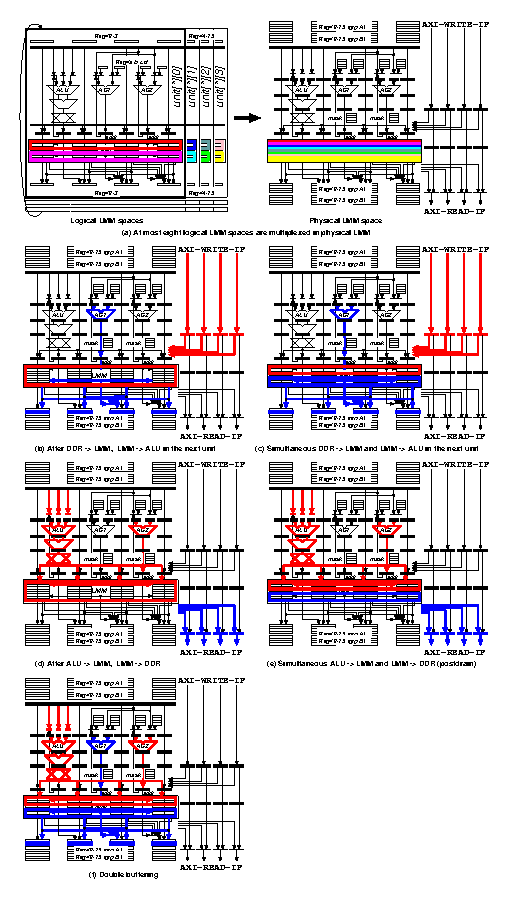
\includegraphics[angle=0,origin=b,width=0.85\textwidth]{lmmmode.eps}
\caption{\label{fig:lmmmode}�����������(LMM)���͡��ʻ�����ˡ}
\end{figure}

��\ref{fig:lmmmode}�ˡ������������(LMM)���͡��ʻ�����ˡ�򼨤���

\begin{description} \parskip 0pc \itemsep 0pc
\item{(a)} ʪ��Ū�ʥ������������֤�����������б����ƣ�ʬ�䤷���ꡤ��ʬ
�䤷����������Ƕ�ͭ�����ꡤʬ�䤻�����ΤǶ�ͭ���뤳�Ȥ��Ǥ��롥ʬ����ˡ�Ϻ�
�ߤ��ǽ���ʤ���Ʊ��LMM�Υץ�ե��å�/�ݥ��ȥɥ쥤��䡤���֥�Хåե����
��ǽ����Ѥ�����ϡ����磸ʬ��Ȥʤ롥

\item{(b)} ���ϥǡ�����DDR����LMM���ɤ߹�����塤LMM����黻�����Ϥ˶��뤹�롥
������̿������֤�����Ρ�LMM�ΰ���Ū�ʻ�����ˡ���ʤ�������LMM�ؤΥץ�ե���
���ȡ���Ҥ�̿��������֥��եȤ��Ȥ߹�碌��ȡ�DDR����LMM�ؤ�ž�����֤�黻
���֤˱��äǤ��롥

\item{(c)} LMM����黻�����Ϥ˶��뤷�ʤ��顤�����IMAX��ư��ɬ�פ����ϥǡ���
��DDR����Ʊ��LMM�����ΰ���ɤ߹��ࡤƱ��LMM���Ф��ơ��黻�Ѥ��ɤ߽Ф��ȥץ�
�ե��å��Ѥν񤭹��ߤ�Ʊ���˹Ԥ�������ˡ��2�Ĥζ��֤�LMM��Ʊ�蘆����Τ�DMA
Ĺ�ϡ�LMM����ʬ���Τ����Ⱦʬ�ˤʤ롥

\item{(d)} �黻��̤�LMM�˽񤭹�����塤���ϥǡ�����LMM����DDR�ؽ��᤹����
�ȥ�̿������֤�����Ρ�LMM�ΰ���Ū�ʻ�����ˡ���ʤ�������LMM����Υݥ��ȥ�
�쥤��ȡ���Ҥ�̿��������֥��եȤ��Ȥ߹�碌��ȡ�LMM����DDR�ؤ�ž�����֤�
�黻���֤˱��äǤ��롥

\item{(e)} �黻��̤�LMM�˽񤭹��ߤʤ��顤����ư���ν��ϥǡ�����Ʊ��LMM��
���ΰ褫��DDR�˽��᤹��Ʊ��LMM���Ф��ơ��黻��̤ν񤭹��ߤȥݥ��ȥɥ쥤��
�Ѥ��ɤ߽Ф���Ʊ���˹Ԥ�������ˡ��2�Ĥζ��֤�LMM��Ʊ�蘆����Τ�DMAĹ�ϡ�LMM
����ʬ���Τ����Ⱦʬ�ˤʤ롥

\item{(f)} DMAĹ��0����ꤹ�뤳�Ȥˤ�ꡤLMM��DDR�δ֤Υǡ���ž�����޻ߤǤ�
�롥���ξ�ǡ���Ϣ�α黻��̤�LMM�˽񤭹��ߤʤ��顤����α黻��̤�Ʊ��LMM��
���ɤ߽Ф��Ƽ��α黻�˻��ѤǤ��롥���ʤ����LMM����֥�Хåե��Ȥ��ƻ��Ѥ�
�뤳�Ȥ��Ǥ��롥FFT��ޡ��������ȤΤ褦��¿�ʽ����Υѥ��ץ饤��¹Ԥ����ѤǤ��롥
\end{description}

\clearpage

\section{��󥰹�¤��UNIT����³��̿��������֥��եȵ�ǽ}

\begin{figure}[htbp]
\center
\epsfile{file=EMAX6RING.eps,width=0.90\textwidth}
\caption{\label{ring}24�Թ����γ���}
\end{figure}

����ʣ��ˤ��б����뤿��ˡ�̿��������֥��եȵ�ǽ��Ƴ����������\ref{ring}�ϡ�
DDR��ޤ�24�Թ����γ��פǤ��롥EMAX5�Ǥϡ������ô������fsm������ʬ�ڤˤ��
��³���줿���Ƥ�LMM�ȼ絭���δ֤ΥС�����ž����Ԥ��Τ��Ф���IMAX�Ǥϡ��ѥ�
�ץ饤�����Х��ˤ��LMM�λ��Ȥ�Ԥ�����ʬ�ڤΤ����������︺�Ǥ����ޤ���
�о�LMM�����ؤ������פǤ��뤿�ᡤDMAž����PIOž���򺮺ߤ������ڤ��ܤʤ��¹�
�Ǥ��롥EMAX5�Ǥ�DMA�Τߤ���Ѥ��Ƥ���conf��lmmi��regv�ν�����ˡ�IMAX�Ǥ�
PIO����ѤǤ�����ʬŪ�ʥ쥸�����������®���Ǥ��롥DMAž���κݤ�UNIT���ٱ��
2�������롤�黻�¹Ի���UNIT���ٱ��8��������Ǥ��롥�ʤ�������Х���1��24
�Թ�������ʣ���������Ȥ��ؤ��뤳�Ȥˤ�ꡤ����Х��ٱ���֤�û�̤Ǥ��롥

̿��������֥��եȵ�ǽ�ϡ���󥰹�¤�����Ѥ���LMM�����Ƥϰ�ư������̿�����
���ž��ư�����롥���襳��ѥ��餬���С����ȱ黻��ư���˥ۥ��Ȥ����̿�᥷��
�Ȼؼ������ɤ��������Ƥ�������ľ�����С����ȱ黻��ư���ˡ����ߤ�LMM�Υ���
�쥹�ϰϤȼ��ΥС����ȱ黻��ɬ�פʥ��ɥ쥹�ϰϤ���Ӥ���Ʊ��ξ���̿�᥷��
�Ȼؼ���ȯ�Ԥ��ʤ��褦���ɤ�����ǽ�Ǥ��롥

\section{����Ȥ��ƤΥ�����������³��ǽ}

\begin{figure}[htbp]
\center

\includegraphics[angle=0,origin=b,width=0.90\textwidth]{mchip.eps}
\caption{\label{fig:mchip}Cascaded peer-to-peer AXI bus for scalable
multichip CGRA}
\end{figure}

����ʣ��ˤ���ӡʣ��ˤ��б����뤿��ˤϡ��ޥ�����å׹�����ͰƤ������ޥ��
���å׹����ˤ�ꥳ���ȥ����󤬿ޤ��Τϡ�ñ����åפ����Ѥ򾮤������뤳�Ȥ�
�����α�ޤ꤬��������뤿��Ǥ��롥AMD��Threadripper��4���åפ�MCM�ˤ���
Intel��Core-i9�ʥ��󥰥���åסˤ�������ʤǤ��뤳�Ȥϵ����˿�������

IMAX�ϡ�ARMv8��ۥ��ȤȤ���ɸ��AXI�Х���Υ���ǥХ����Ȥ���Ǥ�դα黻��
��ARM�μ絭�����־�˼����Ǥ��롥���κݡ����Ĥζ��֤�ʣ����LMM����������ۥ�
�Ȥ����PIO/DMA�ˤ�ꡤ¿����LMM�˲�����ѥ�᥿����Ƥ˽񤭹��ळ�Ȥ��ǽ��
���롥�ץ�����ޤ�C����ˤ�ꥢ�ץꥱ�������򵭽Ҥ���ݡ��ƥǡ�����¤���
��LMM���б��դ��뤫����ꤷ���ǡ�����¤�֤˱黻�����֤���Ǥ�դΥǡ����ե���
������Ǥ��롥�ʤ����ǡ�������ѥ���8���8�Թ����Ȥ���ARM�Ȥδ֤�ž���ٱ��
�㸺���Ƥ��롥���ơ�IMAX�ϡ�IoT�������Ψ������˥����쥤��������졼���Ȥ�
��ɬ�פʵ�ǽ����ܤ��Ԥ������ȹͤ��Ƥ��롥�����������Ѳ��˶�Ť��뤿��ˤϡ�
�͡���IoT���׵���ǽ�˹�碌�ơ���������֥����ǽ�����Ǥ�����ܹ�¤������
�뤳�Ȥ�ɬ�ܤǤ��롥ʣ�����åפˤޤ����ä�¿����LMM�ؤΥ֥����ɥ��㥹��
PIO/DMA���Ǥ����黻��̤β����ʣ�����åפˤޤ����ä�PIO/DMAž���Ǥ���С���
���ѡ����ƥ󥷥�׻�������ǧ����ɬ�פʾ��߹��߱黻�����̤��褯��®���Ǥ��롥
��������GPU�Τ褦��¿���Υ���Х����Ѱդ���������³������ˡ�ϡ�¿����AXI��
�����ѰդǤ��ʤ�IoT������������졼���Ǥ������Ǥ��롥�����ǡ�DMA���졼�ַ���
���뤳�Ȥ����Ѥ���Ʊ��AXI�Х��˥�����������³���ƽ��פ���ǽ����ã�Ǥ��륢��
���ƥ������ͰƤ�����Ʊ�ͤΥ�����������³�����ϡ�����CAM-LSI�����̳�ĥ����
�Ѥ���Ƥ�����ΤΡ���������졼����Ŭ�Ѥ��줿��Ϥ���ޤǤˤʤ�������ϡ�
GPU��Ϥ���Ȥ����̾�Υ�������졼��������å��ʥ���Х����������Ȥ�
��DMA�ޥ����Ȥ����߷פ���뤿��Ǥ��롥

��\ref{fig:mchip}�ˡ�2���å׹����ξ���unit����³��ˡ�򼨤���PIO/DMA��ǽ��
ͭ����ۥ��Ȥ���Ӽ絭����DDR�ˤȡ����å�\#0����ӥ��å�\#1����1�Ȥ�AXI4�Х�
�ˤ�ꥫ����������³����Ƥ��롥64�Ĥ�unit����¢����ƥ��åפϡ��黻�Ѥ�1��
�����Υ����³�ʳ�unit�̲���֤�8��������ˡ�DDR-LMM��ž���Ѥ�8��x8����
�Υǡ����ѥ���Ʊ�ͤ˳�unit�̲���֤�2��������ˤ������Ƥ��롥�黻�Ѥ�DDR-LMM
��ž���Ѥ�ͭ���ʤ��Τϡ��黻��ž����Ʊ��ư��˲ä������å׿����û��������
�ʤ�64unit�̲���֤������︺����������Ǥ��롥AXI-WRITE-IF�ϡ��ۥ��Ȥ���ν�
�������׵����å��⤪��Ӽ����åפ����¤��롥�ޤ�AXI-READ-IF�ϡ����å���8��
����Ӽ����åפ���α������Ԥ���碌�Ʒ�̤��᤹���ʤ��ǽ�Ū�ʥϡ��ɹ����ϡ�
DDR4-3600(64bit)�����å״�ʪ����³��Xilinx�Ҥ�28Gbps-GTY������������������ư
���(4��)x8�ȡ������������å��⥹�롼�ץåȡʸ�ҤΤ褦��
900MHzx256bit=230Gbps�ˤ����礦����Ǥ��롥

\begin{figure}[htbp]
\center
\epsfile{file=EMAX6SEQ.eps,width=0.76\textwidth}
\caption{\label{seq}3Chip������ư��}
\end{figure}

��\ref{seq}�ϡ�3chip������ư��Ǥ��롥DDR�˳�Ǽ����Ƥ������ϲ����ϡ�DMA�ˤ�
�ꡤ���ꥢ����³���줿���Ƥ�IMAX���������졤��IMAX�Ǥϥ��ɥ쥹����˴�Ť���
����LMM�����ϲ�����ΧŪ�˼����ࡥ���κݡ�Ʊ�����ɥ쥹����򥻥åȤ��뤳
�Ȥˤ�ꡤʣ���ս��LMM��Ʊ���˼����ळ�Ȥ��ǽ�Ǥ���ʿ�\ref{seq}(a)�ˡ�
�����LMM���Ф���Write��Ʊ�ͤˡ����ɥ쥹����˴�Ť�������LMM����ΧŪ�˼��
����ʿ�\ref{seq}(b)�ˡ��黻�¹Ի��ϡ���IMAX����Ω�˱黻��Ԥ�����̤�LMM��
��Ǽ����ʿ�\ref{seq}(c)�ˡ��黻��̤Ǥ�����ϲ����ϡ�DMA�ˤ�ꡤLMM����DDR
���ɤ߽Ф����ʿ�\ref{seq}(d)�ˡ�

\begin{table}[htbp]
\center\small
\caption{\label{physinterface}ʪ�����ꥤ�󥿥ե�����}
%%\tabcolsep 0.2pc
\begin{tabular}{l|c|p{4.2in}}\hline\hline
������̾��		& I/O	& ���� \\\hline
rw			& I	& 0:read(LDDMQ/TRANS�Υݡ���󥰴ޤ�), 1:write \\
ty			& I	& 0:reg/conf, 1:reg/breg, 2:reg/addr, 3:lddmq/tr, 4:lmm \\
			&       & read\&lddmq:LMM������ɤ߽Ф�, write\&tr:TR�ؤν񤭹��� \\
col[1:0]		& I	& �������ֹ� \\
sqi[15:0]		& I	& seq�ֹ�ʺ���64Kdwords��\\
avi			& I	& 0:a/dm/di̵��, 1:ͭ�� \\
a[31:5]			& I	& register/LMM�Υ��ɥ쥹 \\
dm[31:0]		& I	& register/LMM�ؤν񤭹��ߥǡ���Byte��ޥ��� \\
di[255:0]		& I	& register/LMM�ؤν񤭹��ߥǡ��� \\
avo			& O	& 0:sqo/do̵��, 1:ͭ�� \\
sqo[15:0]		& O	& seq�ֹ�ʺ���64Kdwords��\\
do[255:0]		& O	& LMM������ɤ߽Ф��ǡ��� \\\hline
\end{tabular}
\end{table}

ɽ\ref{physinterface}�˼���CPU-IMAX��ʪ�����ꥤ�󥿥ե������ϡ�CPU������
����Ȥ���IMAX�򻲾Ȥ���Τ�ɬ�פ����������鹽������롥rw:1bit��R/W���̡�
ty:2bit��register/LMM����col:�������������ֹ�, sqi:16bit��seq�ֹ桤
avi:1bit��R/W�׵ᡤa:27bit�Υ��ɥ쥹����4dword���饤��ˡ�dm:4bit��dwordñ��
�ޥ���, di:256bit�Υǡ�������Write�ˡ�avo:1bit���ɤ߽Ф��ǡ���ͭ��ɽ����
sqo:16bit��seq�ֹ桤do:256bit�Υǡ�������Read�ˤ��ޤޤ�롥

\clearpage

\section{�ܺٹ�¤��ư��}

\begin{figure}[htbp]
\center
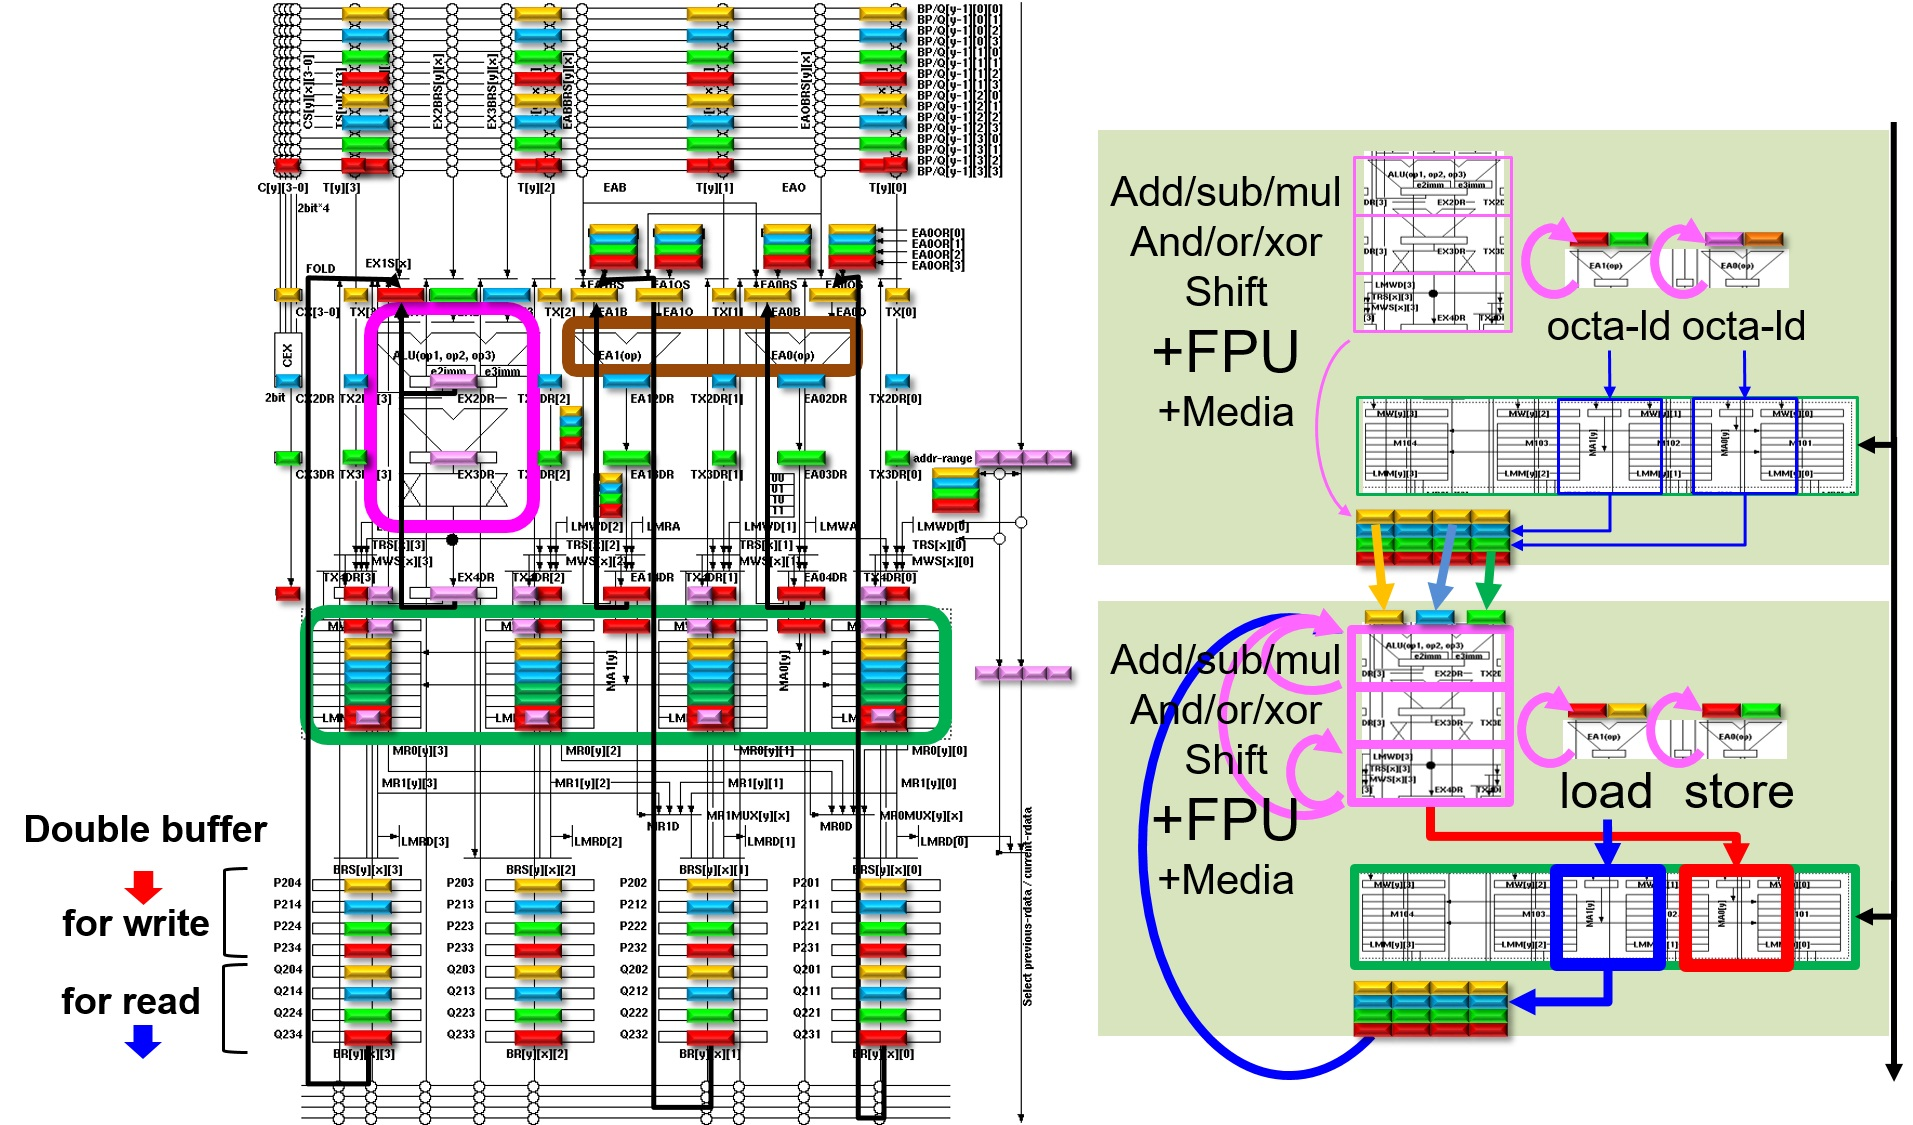
\includegraphics[angle=270,origin=b,width=0.98\textwidth]{IMAX1.eps}
\caption{\label{imax1}IMAX�δ���UNIT��¤}
\end{figure}

\begin{figure}[htbp]
\center
\epsfile{file=EMAX6EXE.eps,width=0.98\textwidth}
\caption{\label{exe}UNIT��黻��ι����ȥ����ߥ�}
\end{figure}

\begin{figure}[htbp]
\center
\epsfile{file=EMAX6LMM.eps,width=0.98\textwidth}
\caption{\label{lmm}UNIT�������������LMM�ˤι����ȥ����ߥ�}
\end{figure}

\begin{figure}[htbp]
\center
\epsfile{file=EMAX6PMM.eps,width=0.98\textwidth}
\caption{\label{pmm}CPU����Υ�����������LMM��ľ�ܻ���}
\end{figure}

��UNIT�α黻��ˤϡ������黻��ñ������ư�������黻����ӥޥ����ǥ����黻��
���Ƥ��롥��\ref{exe}�ϡ��黻������ܤ����쥸�������ȤΥ����ߥ󥰥��㡼�Ȥ�
���롥4��ʬ�α黻��ǽ��1��ʬ�Υϡ��ɥ��������Ѥ���¿�ż¹Ԥˤ��¸����Ƥ��롥
�쥸�����ɤ߽Ф��ȱ黻��4���������ʬ�䤷�ƥѥ��ץ饤��¹Ԥ��롥��\ref{lmm}
�ϡ�LMM�����ܤ����쥸�������ȤΥ����ߥ󥰥��㡼�ȤǤ��롥Ʊ�ͤ�4��ʬ��LMM��
ǽ��1��ʬ�Υϡ��ɥ��������Ѥ���¿�ż¹Ԥˤ��¸����Ƥ��롥LMM�����4ʬ�䤷
��4�Ĥλ��Ȥ�ѥ��ץ饤��¹Ԥ��롥LMM��ʬ�䤷�ʤ���硤EA0/1�ν���18bit����
�Τޤ�LMM�Υ��ɥ쥹����˻��Ѥ���롥LMM��4ʬ�䤹���硤EA0/1�ν���18bit��
���2bit�����ֹ�˱�����00/01/10/11�Τ����줫�˾�񤭤���LMM�Υ��ɥ쥹�����
���Ѥ���롥��\ref{pmm}�ϡ�CPU����LMM��ľ�ܻ��Ȥ�����˻��Ѥ���DMA/PIO�Υǡ�
���ѥ������Ǥ��롥���Ԥ����襵�����롤���ɥ쥹��R/W���̡��񤭹��ߤξ���
���ߥǡ����򶡵뤷��ʣ���Ԥ��鹽������������֤�ѥ��ץ饤��Ū�˻��Ȥ���
�ǽ��Ԥ����ɤ߽Ф��ǡ�������Ф����ɤ�UNIT��LMM����Ū���ɥ쥹����Ƥ��Ƥ�
�뤫�ϡ����ɥ쥹�ȳ�UNIT��vAddr-range��top,len�ˤ���Ӥˤ��Ƚ�ꤷ����LMM��
���פ��Ƥ������R/Wư���Ԥ����ɥ쥹����ӥǡ����򼡹Ԥ��Ϥ����԰��פξ�
��⥢�ɥ쥹����ӥǡ����򼡹Ԥ��Ϥ���

\clearpage

\begin{figure}[htbp]
\center
\epsfile{file=EMAX6MAP.eps,width=0.98\textwidth}
\caption{\label{emax6map}UNIT�ε�ǽ}
\end{figure}

��\ref{emax6map}(a)����(j)�ϡ�UNIT�˼�����ǽ�ʵ�ǽ�Ǥ��롥(a)�ϡ����μ¹Ԥ�
ɬ�פʼ絭������Υǡ�����LMM�˥ץ�����ɤ��Ĥġ������ɺѥǡ�����LDRQ
��4dwords��/LDR��1dword�ˤ����Ԥα黻��˶��뤹�롥�ץ�����ɤˤϡ�blk��0:��
���å���̵����1:16��Ϣ³���������Ƭ�ݥ��������ʤ��֥��å��󥰡�2:32
��Ϣ³���������Ƭ�ݥ��������ʤ��֥��å��󥰡�3:64��Ϣ³���������Ƭ��
���������ʤ��֥��å��󥰡ˤ����len��32bitñ�̤ΥС�����Ĺ�ˤ���ꤹ�롥

(b)�ϡ��黻��̤�STRQ��4dwords��/STR��1dword�ˤˤ��LMM�˥��ȥ����Ĥġ�����
�μ¹Է�̤�絭����ž�����롥STRQ������Ū��ʣ����α黻��̤�LMM�˳�Ǽ����
����ˡ�1�����������1dword���Ǽ���롥���Τ��ᡤƱ��Ԥ�ʣ����STRQ��ץ����
�ɤ�������뤳�ȤϤǤ��ʤ���

(c)�ϡ�Ʊ��UNIT�ˤ�����LMM��read-modify-write��ԤäƤ��롥top��blk��len�ˤ�
����ꤵ�줿�ϰϤ�ͽ��LMM�˳�Ǽ���롥���θ塤LDRQ���ɤ߽Ф����ǡ������黻��
���Ϥ��ᤵ�졤��̤�Ʊ��LMM�˽��ᤵ��롥�ޥ������åǥ��󥰵�ǽ�ˤ�ꡤ
���Τ褦�ʥ������졼�Ȥ�������Ƥ�ѥ��ץ饤�󤬻ߤޤ뤳�ȤϤʤ���

(d)�ϡ�LDR��LMM��������ɤ���Τ���Ω����top��blk��len�ˤ����ꤵ�줿�ϰϤ�
ͽ��LMM�˳�Ǽ���롥���θ塤LDR�������ॢ�ɥ쥹����˴�Ť�LMM�򻲾Ȥ��롥
top��blk��len��Ʊ���LDR�ϡ�LMM�Υǥ奢��ݡ��ȵ�ǽ�����Ѥ��졤Ʊ��UNIT
�˼�������롥

(e)�ϡ�(d)���Ф�ʤ����黻��̤�STR�ˤ��LMM�˥��ȥ����Ƥ��롥���ƤΥ��ȥ���
��λ�塤LMM����絭����len�ˤ����ꤵ�줿�̤Υǡ������С�����ž������롥

(f)�ϡ��ȥ�󥶥������Ǥ��롥�黻��̤�TR��4dwords�ˤˤ��LMM�˥��ȥ�����
�ġ�ARM�˥ȥ�󥶥�������ɬ�פ�4dwords�򶡵뤹�롥TR������Ū��ʣ����α黻
��̤�LMM�˳�Ǽ���뤿��ˡ�1�����������1dword���Ǽ���롥���Τ��ᡤƱ��Ԥ�
ʣ����TR��ץ�����ɤ�������뤳�ȤϤǤ��ʤ���

(g)�ϡ��������꤫���ľ�ܥ����ɵ�ǽ�Ǥ��롥�絭�����ɥ쥹�׻���EX�˼�����
�졤���ɥ쥹��LMM��dword0�˥��塼���󥰤���롥LMM�񤭹����Ѥˤ�EA0����Ѥ���
ARM������AXRA��EA0��Ʊ���͡ˤ�ƻ뤷���������ɥ쥹����Ͽ���Τ���LMM�����
�������ɥ쥹����Ф���AXI����Ѥ��Ƽ絭�����ɤ߽Ф���LMWD�˥ǡ��������Ф�
�롥UNIT�Ǥϡ�LMWD��TR��BR���ͳ����4dword�򼡹Ԥ����Ф��롥

�Ȥ����ǡ��ʾ�δ��ܵ�ǽ�Τ�����(g)�μ����˺ݤ��Ƥϡ��絭���ٱ���Ф����θ
��ɬ�פǤ��롥�ץ�����ߥ󥰻����ü�ʵ��Ҥ�ɬ�פȤ��ʤ���ΤΡ��������ˤϡ�
(g)��Ʊ��Ԥ˴ޤޤ��UNIT�Ǥϡ�(h)�Τ褦��LMM�����Ѥ����ٱ�Ʊ����������
��������롥Ʊ�ͤˡ��쥸���������¤�ɬ�פǤ����硤�����쥸��������Ѥ��ơ�
(i)���ٱ�Ʊ��̵�ˤ�(j)���ٱ�Ʊ��ͭ�ˤΤ褦�ʵ�ǽ����������롥

\section{���ߥ�졼��}

��®�������Τʥץ��ȥ����׳�ȯ�Τ���ˤϡ��ޤ���Verilog�ˣ��У����Ѵ���ǽ��
��٥�ξܺ٥��ߥ�졼���γ�ȯ��ɬ�ܤǤ��롥����ϡ�Verilog���ߥ�졼����ư
��®�٤��ˤ���٤�����ˡ��絬�Ϥʥ��ץꥱ��������ư��ڤ�����Ǥ��뤳�ȡ�
�ޤ���Verilog���ߥ�졼���ˤ��ϡ��ɥ������߷׸��ڤΤ���ˤϡ��쥸�����ͤ�
�����ͤȤ���Ӥ�Ԥ���������Τʴ����ͤ�ɬ�ܤʤ��Ȥˤ�롥IMAX�������ARMv8
�ˤ��Ԥ����ᡤARMv8�⥷�ߥ�졼������ǽ��IMAX���ߥ�졼����ȯ������C��
��ˤ�17K�Ԥε��ϡˡ����ҤΥ��ץꥱ�������ץ�����ࡤIMAX����ѥ��顤����
�ӡ��ܥ��ߥ�졼�����Ѥ��ơ��ץ��ȥ����ץ����ƥ���߷׳������ˡ��ϡ��ɥ�����
�ǥХå���ɬ�ܤδ�������ӵ�ǽ�դ��ƥ��ȥץ�����प���Verilog���ߥ�졼����
���ѥƥ��ȥ٥�������������

\section{FPGA�ˤ��ޥ�����åץץ��ȥ�����}

\begin{figure}[htbp]
\center
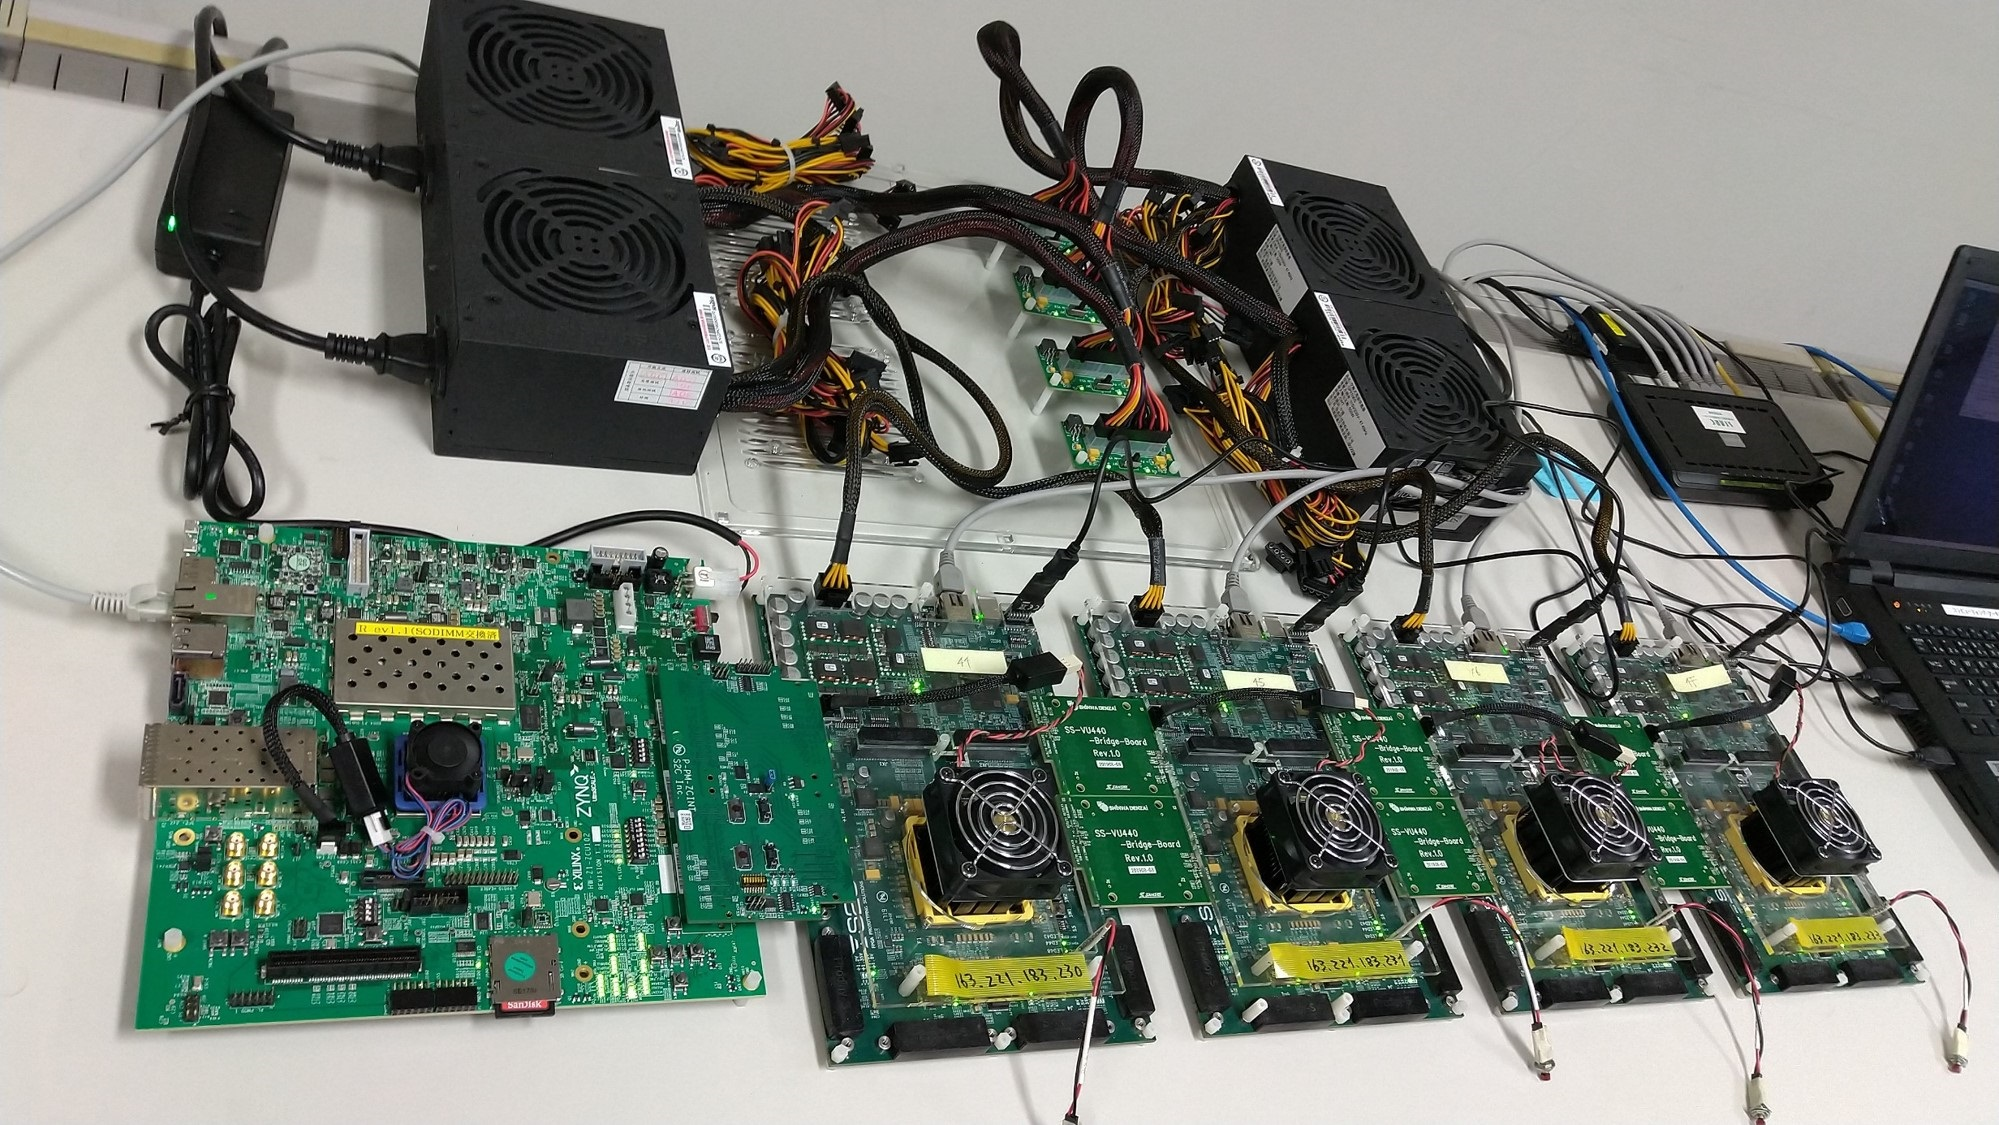
\includegraphics[angle=270,origin=b,width=0.98\textwidth]{IMAX4.eps}
\caption{\label{imax4}4���å׹�����IMAX}
\end{figure}

8���å׹�����µ�ɾ�����뤿��ˤϡ�XILINX����VU440��8����ܤ����Ķ���ɬ
�פǤ��롥���ҤΥ��ߥ�졼���򸵤�Verilog���Ҥ������������ߥ�졼���ˤ��
���������ƥ쥸�����������ͤ�Verilog���ߥ�졼������̤���Ӥ��ƥǥХå���
�ʤ᤿���ϡ��ɥ����������̤ϡ�Verilog�ˤ�11K�ԤǤ��ä����ۥ��Ȥˤϡ����å���
�Х�������CPU�ζȳ�ɸ��Ǥ���ARMv8����ܤ���Xilinx����Zynq UltraScale+
��ZCU102�ˡ�IMAX�ˤϡ�S2C����Virtex Ultra Scale��S2C Single VU440 Prodigy
Logic Module�ˤ���Ѥ����ʿ�\ref{imax4}�ˡ����ߤǤ⡤64unit������IMAX�����
��ǽ��FPGA��VU440�ΤߤǤ��ꡤARMv8��VU440���®���ꥢ���󥯤ˤ����³��ǽ
�ʥ����ƥ�Ȥ������Ȥ߹�碌�Ϻ�Ŭ�Ǥ��롥�������������������ڥå���ϡ�
10Gbps�ι�®���ꥢ���󥯤�3��«�ͤ�30Gbps�Υ��롼�ץåȤ��Ф���Ϥ��ʤΤ�
�Ф����ºݤˤϡ�5Gbps x 3�졼��ι��15Gbps�Υ��롼�ץåȤǤ�����󥯤��Ω
�Ǥ��ʤ��ä��ʤ��θ�8�졼�����®�ˡ��ޤ���8���åפ���³����ȡ�LMM�������
�߽Ф��˻��Ѥ���AXI-READư��ˤ����®�Ǥ��뤳�Ȥ�Ƚ������������ϡ��ۥ���
��DMA��ǽ���Ф��ƽ�ʬ��Ĺ���ΥС�����Ĺ����ꤷ�Ƥ⡤�ۥ��Ȥ���¢����Ƥ���
AXI���󥿥ե�������AXI3�ߴ��Ǥ��ꡤ256bit��ž���ξ�硤8beat���Ȥ�ž����ʬ��
���졤�����åפ���α�������λ����ޤǼ���AXI-READ���Ԥ�����뤳�Ȥ������Ǥ���
���������ǡ��ѹ��Ǥ��ʤ��ۥ��Ȥ�AXI���󥿥ե�������AXI3�Τޤ޻��Ѥ��Ĥġ�
IMAX�֤Ǥ�ʬ�Ǥ����˸��ΥС�����Ĺ��ݻ����뵡����ͰƤ���AXI-READ�������ʹ�
®��������������

\section{����ɾ��}

\begin{figure}[htbp]
\center
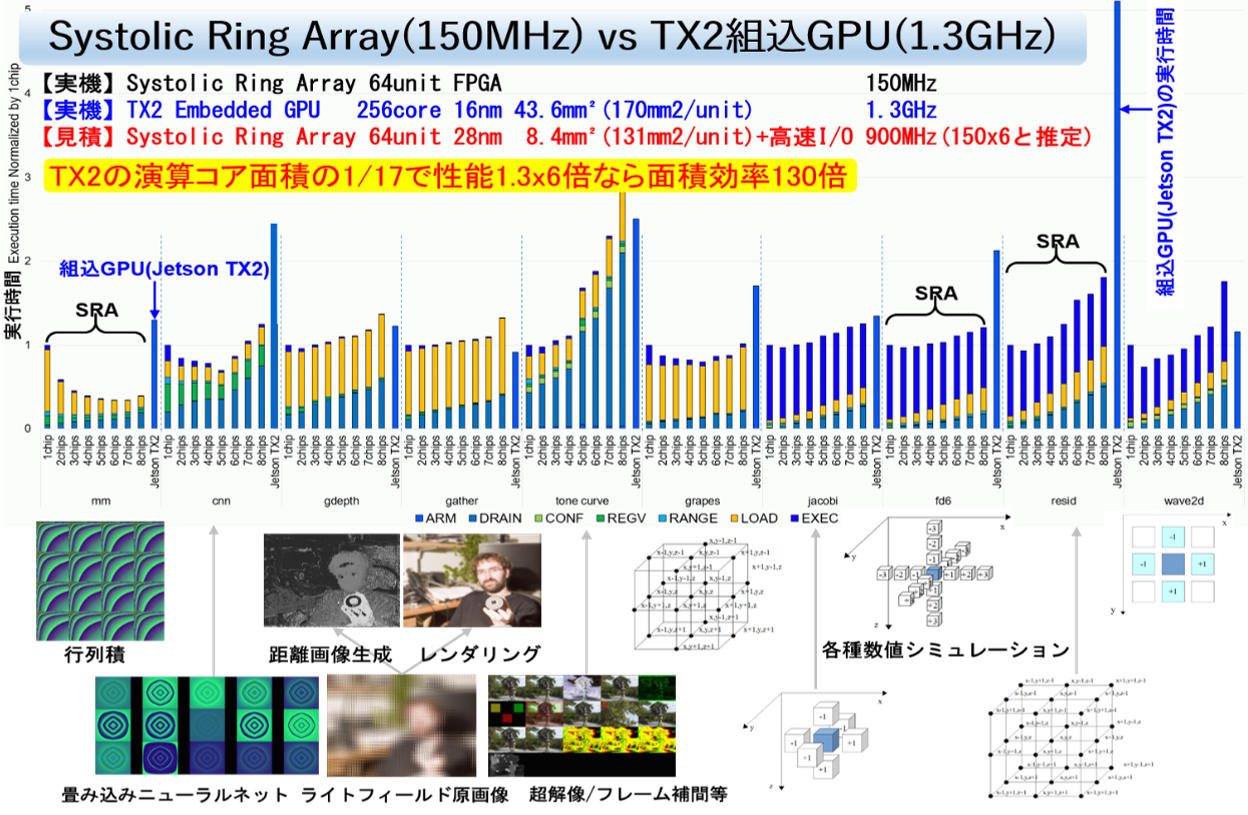
\includegraphics[angle=270,origin=b,width=0.98\textwidth]{result1.eps}
\caption{\label{result1}����ɾ��1 (15Gbps interface)}
\end{figure}

\begin{figure}[htbp]
\center
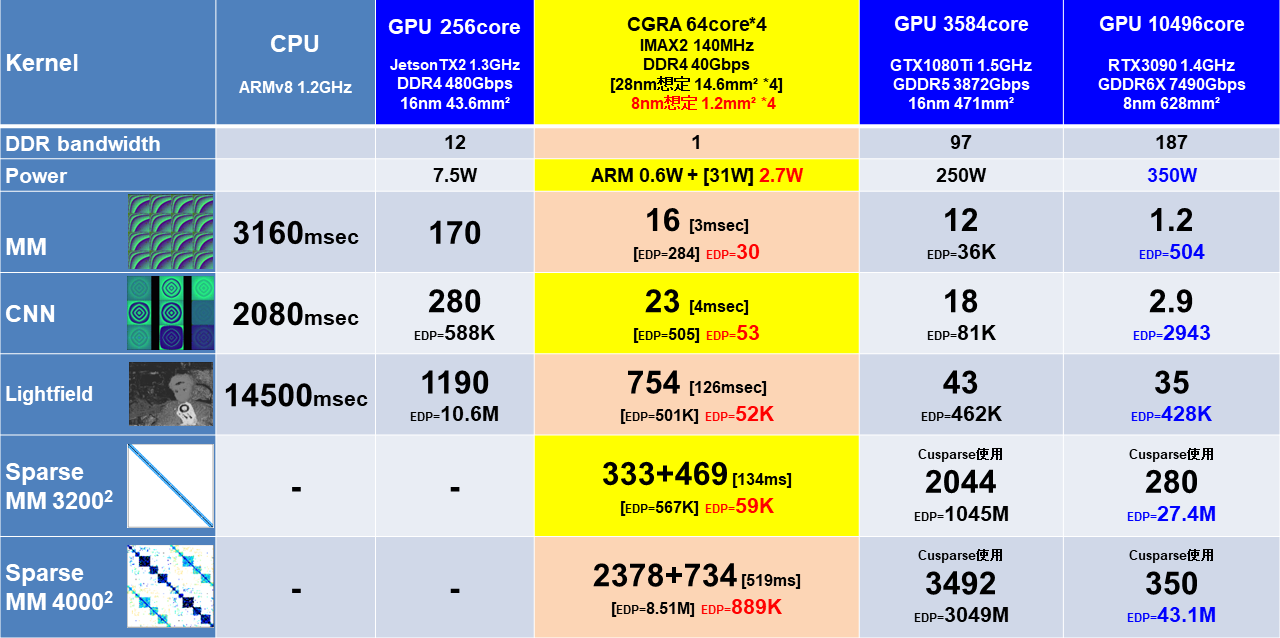
\includegraphics[angle=270,origin=b,width=0.98\textwidth]{result2.eps}
\caption{\label{result2}����ɾ��2 (40Gbps interface)}
\end{figure}

�ʾ�ηаޤ�ФƳ�ȯ����λ����IMAX��8���å׹�����ǥ���Ѥ��ơ��Ƽ�ץ�����
������Ԥ���������\ref{result1}�ϡ�5Gbps��Aurora���󥿥ե�������3�졼�����
��(��15Gbps)��IMAX�Υ��å׿���1����8�ޤ��Ѳ�������¬�ꤷ�����ץꥱ��������
�¹Ի��֤Ǥ��롥�ץ��������ˡ�1���å׹�����ư����ȿ�150MHz���黻���64��
���Ѥ�28nm�ˤƿ���8.4mm2�ˤμ¹Ի��֤�������������Ƥ��ꡤ��ӤΤ���ˡ���
�߹���GPGPU(Jetson TX2��ư����ȿ�1.3GHz���黻���256���黻������ʬ�����Ѥ�
16nm�ˤƿ���43.6mm2)�μ¹Ի��֤�Ǻܤ��Ƥ��롥������(mm)��7chipϢ�롤���߹�
��(cnn)��5chipϢ�롤��Υ����(depth)��2chipϢ�롤�ʳص��ѷ׻�(Stencil�׻�)��
�ϡ��絤���ߥ�졼�����(grapes)��5chipϢ�롤����¾���ƥ󥷥��2chipϢ�뤬��
®�Ǥ��ä������Τη����Ȥ��ơ�mm��cnn�Τ褦��chip�ֶ��̥ǡ�����¿���ȥޥ��
���åײ��θ��̤��礭�������ƥ󥷥�Τ褦��ñ��ʶ���ʬ��Ǥϸ��̤��������ʥ�
���Х�����������ޤޤǤΥޥ�����åײ���ɬ�פʤ��ˤ��Ȥ��狼�롥�����ơ�����
���ǥХ�������θ¤�줿����Х����(Jetson TX2��1/32)�Ǥ�Ǽ���Ǥ����̤�
����줿����\ref{result2}�ϡ�5Gbps��Aurora���󥿥ե�������8�졼�����
(40Gbps)����ɾ���Ǥ��롥1.3GHzư���Jetson TX2��140MHzư���IMAX����ǽ�̤�ο
�路�Ƥ��뤳�Ȥϡ�CGRA�Υݥƥ󥷥���ʬ�˼����Ƥ��롥�ޤ���IMAX������28nm
��ASIC���ˤ��900MHzư�����硤Jetson TX2��1/17�����ѤǺ���15��(1���å׹�
����cnn�ξ��)����ǽ�Ȥʤꡤ���Ѥ�������ǽ�Ǥ�250�ܤȤʤ롥�������Ϥ����Ѥ�
���㤹��ȹͤ���ȡ�Ʊ����ǽ������ξ������Ϥ�Ʊ����Ψ�Ǥ���ȹͤ����롥


\chapter{IMAX Software}

\section{�絭����˼��������IMAX���󥿥ե�����}

\begin{figure}[htbp]
\center
\epsfile{file=EMAX6MMAP.eps,width=0.98\textwidth}
\caption{\label{mmap}ʪ���������}
\end{figure}

��\ref{mmap}��CPU��ʪ��������֤򼨤���IMAX�˴�Ϣ����ʪ��������֤ϡ�
��1��CPUʪ��������֤�LMM�δ֤�DMA�����椹��FPDDMA-CH1 DMA����쥸��������
��DMA control register space:4KB�ˡ���2��LMM��CPUʪ��������֤˼�������DMA
�ˤ�껲�Ȥ���LMM DMA���֡�pAddr2 space:2GB�ˤ����IMAX��Υ쥸������PIO��
��껲�Ȥ�������쥸�������֡�pAddr2+ space:2GB�ˡ���3��LMM�Ȥ�DMA����ǽ��
DDR������֡�pAddr space:2GB�ˤ��鹽������롥���Τ�����IMAX�Ȥ�ʪ��Ū��
³�ˤ�껲�ȤǤ�����֤ϡ�pAddr2 space:2GB�����pAddr2+ space:2GB�Ǥ��롥
IMAX��LMM�������̤�16MB��256KB*64stages�ˡ��ǡ����Х�����256bit��32B�ˤǤ�
�뤿�ᡤ���ʤ��Ȥ⥢�ɥ쥹����19bit��1dword��64bit�����1bit�񤭹��ߥޥ�����
4bit��ɬ�פǤ��롥���������쥸�������֤�ä���ʪ��������֤���CPU��ʪ��
������֤˼�������롥

\begin{table}[htbp]
\center\footnotesize
\caption{\label{logicinterface}�������󥿥ե�����}
\tabcolsep 0.2pc
\begin{tabular}{l|c|l|p{3.4in}}\hline\hline
����쥸��������(pAddr2+)	& R/W	& Bit����    & ���� \\\hline
STATUS				&	&	     & \\
0x400000007-0x400000000		& R	& bit3-0     & EXRING���� 0:IDLE, 1:BUSY(SCON/EXECư����) \\
				&  	& bit7-4     & LMRING���� 0:IDLE, 1:BUSY(PIO/DMAư����) \\
				&  	& bit11-8    & 0:EMAX\_DEPTH=8,  1:EMAX\_DEPTH=16 \\
				&  	&            & 2:EMAX\_DEPTH=32, 3:EMAX\_DEPTH=64 \\
				&  	& bit15-12   & 0:LMM\_SIZE=32KB, 1:LMM\_SIZE=64KB, 2:LMM\_SIZE=128KB \\
				&       & bit63-16   & reserved by 0 \\\hline
COMMAND				&	&	     & IMAX�ؤλؼ� \\
0x400000017-0x400000010		& W	& bit1-0     & 0:NOP, 1:RESET, 2:SCON, 3:EXEC \\
				&       & bit31-2    & reserved by 0 \\
				&       & bit35-32   & chip�ֹ�(0��񤭹����chip�֤�缡����)\\
				&       & bit63-36   & reserved by 0 \\\hline
ADRTRANS			&	&	     & vAddr-pAddr2 \\
0x400000027-0x400000020		& W	& bit63-0    & DDR-LMM��DMA���Υ��ɥ쥹�Ѵ����� \\\hline
COLSELECT			&	&	     & vAddr-pAddr2 \\
0x400000037-0x400000030		& W	& bit1-0     & DMA/LDDMQ/TRANS��������Ū����col���� \\
				&       & bit63-2    & reserved by 0 \\\hline
CONF	  			& 	&            & \\
0x40000201f-0x400002000		& W 	& bit255-0   & ����UNIT\#0.0��conf \\
0x40000203f-0x400002020		& W 	& bit255-0   & ����UNIT\#0.1��conf \\
:                            	& :	&            & : \\
0x400003fff-0x400003fe0		& W 	& bit255-0   & ����UNIT\#63.3��conf \\\hline
REGV-BR				&	&            & BR�񤭹��� \\
0x40000401f-0x400004000		& W	& bit255-0   & ����UNIT\#0.0��BR[3:0] \\
0x40000403f-0x400004020		& W	& bit255-0   & ����UNIT\#0.1��BR[3:0] \\
:				& :	&            & : \\
0x400005fff-0x400005fe0		& W	& bit255-0   & ����UNIT\#63.3��BR[3:0] \\\hline
REGV-EAR/vAddr-range		&	&            & EAB,EAO�񤭹��� \\
				&	&            & LMM��Ƭaddr(max2GB),LMMͭ��dword��(max8KDW) \\
0x40000600f-0x400006000		& W	& bit49-32,17-0   & ����UNIT\#0.0��ea0o,ea0b(virt-addr)    \\
				&  	& bit113-96,81-64 & ����UNIT\#0.0��ea1o,ea1b(virt-addr)    \\
0x400006017-0x400006010		& W	& bit30-0    & ����UNIT\#0.0��top(virt-addr)    \\
				&  	& bit62-32   & ����UNIT\#0.0��bot(virt-addr)    \\
0x40000602f-0x400006020		& W	& bit49-32,17-0   & ����UNIT\#0.1��ea0o,ea0b(virt-addr)    \\
				&  	& bit113-96,81-64 & ����UNIT\#0.1��ea1o,ea1b(virt-addr)    \\
0x400006037-0x400006030		& W	& bit30-0    & ����UNIT\#0.1��top(virt-addr)    \\
				&  	& bit62-32   & ����UNIT\#0.1��bot(virt-addr)    \\
:				& :	&            & : \\
0x400007fef-0x400007fe0		& W	& bit49-32,17-0   & ����UNIT\#63.3��ea0o,ea0b(virt-addr)   \\
				&  	& bit113-96,81-64 & ����UNIT\#63.3��ea1o,ea1b(virt-addr)   \\
0x400007ff7-0x400007ff0		& W	& bit30-0    & ����UNIT\#63.3��top(virt-addr)   \\
				&  	& bit62-32   & ����UNIT\#63.3��bot(virt-addr)   \\\hline
LDDMQ/TRANS-R			&	&	     & LMM����LDDMQ/TRANS�׵���ɤ߽Ф� \\
0x40000801f-0x400008000		& R	& bit255-0   & ����UNIT\#0.0��LMM \\
0x40000803f-0x400008020		& R	& bit255-0   & ����UNIT\#0.1��LMM \\
:                            	& :	&            & : \\
0x400009fff-0x400009fe0		& R	& bit255-0   & ����UNIT\#63.3��LMM \\\hline
LDDMQ-W				&	&	     & TR�ؤν��ᤷ \\
0x40000801f-0x400008000		& W	& bit255-0   & ����UNIT\#0.0��TR \\
0x40000803f-0x400008020		& W	& bit255-0   & ����UNIT\#0.1��TR \\
:                            	& :	&            & : \\
0x400009fff-0x400009fe0		& W	& bit255-0   & ����UNIT\#63.3��TR \\\hline\hline
LMM����(pAddr2)			& R/W	& Addr����   & ���� \\\hline
0x4ffffffff-0x480000000		& R/W	& 32B        & DDR-High(0x87fffffff-0x800000000)���б����֤˳�������LMM�����Ƥ�R/W���롥\\\hline
\end{tabular}
\end{table}

ɽ\ref{logicinterface}��ʪ�����ꥤ�󥿥ե��������̤����󶡤����������󥿥ե���
���򼨤���ʪ��������֤Τ���0x4ffffffff-0x480000000��pAddr2�ˤϡ�
0x87fffffff-0x800000000��pAddr�ˤ��б��դ�����DDR-High��LMM�Ȥδ֤�DMA�Τ�
���FPDDMA���������Ѥ���Ϣ³ʪ�����֤Ǥ��롥�桼���ץ������ϡ�Ϣ³ʪ������
��pAddr2�ˤ�mmap()�ˤ��������Ϣ³���۶��֡�vAddr2�ˤ�PIO�ˤ�껲�Ȥ��뤳
�ȤϤʤ�����顤DDR-HighϢ³ʪ���ΰ��pAddr�ˤ�mmap()�ˤ��������Ϣ³����
���֡�vAddr�ˤΤߤ򻲾Ȥ��롥����Ū�ˤϡ�IMAX���黻��Ϣư����LMM�򻲾Ȥ����
�ˤ�vAddr����Ѥ���LMM����DDR-High���������ɥ쥹��Ʊ�����Ƥ����뤿��ˡ�CPU
�ϡ����餫����vAddr�����Ƥ�LMM��ž�����Ƥ���ɬ�פ����롥ž����LMM������ϡ�
UNIT����ߤ�����vAddr-range�쥸�����Ȥ���Ӥˤ��Ԥ�졤�񤭹����襢�ɥ�
���ˤϡ�FPDDMA����FSM�����Τ����pAddr2��FSM�⥢�ɥ쥹�Ѵ��쥸��������
��vAddr-pAddr2�ˤ˲ä���������vAddr�����Ѥ���롥��UNIT���ߤ�����
vAddr-range�쥸�����ϡ���UNIT��conf.mapdist�ͤ�SCON�ؼ���˸��������ǿ�����
��UNIT�ֹ���б��դ����롥���Τ��ᡤ̿�᥷�եȤ�ȼ�ä�LMM������Ū�˺�����
����Ƥ�����֤Ǥϡ�������ͭ���ˤʤ�LMM�˳�������vAddr-range�쥸�����ν񤭹�
�ߤΤߤ�Ԥ��Ф褤��

\begin{figure}[htbp]
\center
\epsfile{file=EMAX6PROC.eps,width=0.98\textwidth}
\caption{\label{proc}��ư���齪��ޤǤμ��}
\end{figure}

\begin{figure}[htbp]
\center
\epsfile{file=EMAX6LMRING.eps,width=0.98\textwidth}
\caption{\label{lmring}�������󥿥ե������ȳƹԤˤ�����ǡ��������ߵ����δط�}
\end{figure}

��\ref{proc}�ϡ�EMAX5��IMAX�ε�ư���齪��ޤǤ�ư��פ���ӤǤ��롥EMAX5
�ξ�硤CPU��HPM���ͳ����EMAX���FSM��ư����IDLE���֤�CPU�����Τ����ޤ�
FSM��AXI-MASTER�Ȥ���ư��롥������IMAX�ξ�硤CPU¦��AXI-MASTER�Ȥʤꡤ
FSM��AXI-SLAVE�Ȥ���ư��롥DRAIN��LOAD�ˤ�FPDDMA��DMA-CHAIN��ǽ����Ѥ���
CONF��SCON��REGV��RANGE��EXEC�ˤ�PIO����Ѥ��롥EMAX5������֤���Ƥ���LMMI
�ϡ�IMAX�Ǥ�CPU���������Ƥ��ꡤIMAX�ؤ����������פǤ����ΤΡ�������
vAddr-range�ι�����RANGE�ˤ�ɬ�פȤʤ롥��\ref{lmring}���Ѥ��ơ���\ref{proc}
�˼������Ƽ��ˤ�����ϡ��ɥ�������ư����������롥�ʤ���CONF��SCON��REGV��
���RANGE��ñ��ư��Τ߲�ǽ�Ǥ��ꡤEXEC��DMA�ϡ�Ʊ��ư���EXEC��ư���DMA��
ľ���˵�ư�˲�ǽ�Ǥ��롥

\begin{description}
\itemsep 0in
\parskip 0in
\item[RESET] CPU�ϡ�COMMAND��RESET��񤭹��ळ�Ȥˤ�ꡤIMAX�������֤ν��
��������ӡ���UNIT��physical stage\#�ʸ����͡ˤ�logical stage\#�˽񤭹����
������Ԥ����ʤ����ܵ�ǽ��IMAX��ȯ���ΥǥХå��ѤǤ��ꡤ�桼���ץ�����ब
���Ѥ���ɬ�פϤʤ���IMAX��RESETư����ξ�硤STATUS.EXRING��BUSY��ɽ������
�롥

\item[CONF] CPU�ϡ�STATUS.EXRING�����STATUS.LMRING��IDLE�λ���PIO�ˤ��Ϣ³
Ū��CONF�򹹿����뤳�Ȥ��Ǥ��롥CONF������UNIT�ֹ���б�����ʪ�����ɥ쥹����
�����Ƥ��Ƥ��ꡤ����ʪ�����ɥ쥹���Ф��ƽ񤭹��ळ�Ȥˤ�ꡤ�������ֹ�
��pAddr2+��bit12-7�ˤ˰��פ���logical stage\#��ͭ��������UNIT��CONF��������
��롥IMAX��CONF�񤭹���ư����ξ�硤STATUS.LMRING��BUSY��ɽ������롥

\item[SCON] CPU�ϡ�STATUS.EXRING��IDLE�λ���COMMAND��SCON��񤭹��ळ�Ȥˤ�
�ꡤ���Ԥ��Ф��ơ��ƹԤ��ݻ�����conf.mapdist���ͤ˽���CONF�Υ��եȳ��Ϥ�ؼ�
���뤳�Ȥ��Ǥ��롥���ƤιԤϡ���1���������ܤˡ���CONF�����256bit*4set�ˤΤ�
����Ƭ256bit��BR�˽񤭹��ߡ���2���������ܤˡ����Ԥ�BR�������Ԥ�CONF�����
�Ԥ˼����ࡥ�ʾ��4�󷫤��֤����Ȥˤ�����Ƥ�CONF�����1��ʬ�����˥��եȤ�
�롥�ޤ���logical stage\#���ͤ�1���������롥����ˡ��ʾ��conf.mapdist�󷫤�
�֤����Ȥˤ�����Ƥ�CONF�����conf.mapdist��ʬ���եȤ���logical stage\#����
��conf.mapdist���������롥�ʤ���SCON�ˤ��REGV�����Ƥ��˲�����롥IMAX��
SCONư����ξ�硤STATUS.EXRING��BUSY��ɽ������롥

\item[REGV] CPU�ϡ�STATUS.EXRING�����STATUS.LMRING��IDLE�λ���PIO�ˤ��Ϣ³
Ū��REGV-EAR�����REGV-BR�򹹿����뤳�Ȥ��Ǥ��롥REGV������UNIT�ֹ���б���
��ʪ�����ɥ쥹��������Ƥ��Ƥ��ꡤ����ʪ�����ɥ쥹���Ф��ƽ񤭹��ळ�Ȥˤ�
�ꡤ�����������ֹ��pAddr2+��bit12-7�ˤ˰��פ���logical stage\#��ͭ��������
UNIT��REGV����������롥IMAX��REGV�񤭹���ư����ξ�硤STATUS.LMRING��BUSY
��ɽ������롥

\item[RANGE] CPU�ϡ�STATUS.EXRING�����STATUS.LMRING��IDLE�λ���PIO�ˤ��Ϣ
³Ū��vAddr-range�򹹿����뤳�Ȥ��Ǥ��롥vAddr-range������UNIT�ֹ���б�����
ʪ�����ɥ쥹��������Ƥ��Ƥ��ꡤ����ʪ�����ɥ쥹���Ф��ƽ񤭹��ळ�Ȥˤ�ꡤ
�����������ֹ��pAddr2+��bit12-7�ˤ˰��פ���logical stage\#��ͭ��������UNIT
��vAddr-range����������롥�ʤ���LMM��̵����ʬ��̵��2ʬ�䡤4ʬ��Τ����줫��
���ꤹ��ؼ���conf.lmm\_mode�ˤϡ����Ҥ�CONF�˴ޤޤ�롥IMAX��vAddr-range��
������ư����ξ�硤STATUS.LMRING��BUSY��ɽ������롥

\item[DMA] CPU�ϡ�STATUS.LMRING��IDLE�λ���DMA�ˤ��Ϣ³Ū��DDR-LMM��ž����
��ư�Ǥ��롥EMAX5�Ǥ�fsm�ˤ��¸�����Ƥ�����ǽ��IMAX�Ǥ�CPU��DMA���Ѥ��ƹ�
��������Ū�ˤϡ���lmmi�ȿ�lmmi����Ӥ�����lmmi���񤭹����衤�ޤ��ϡ���lmmi��
����STORE�оݡʼ�����Ƭ���ɥ쥹���ۤʤ�lmx�ˤλ�������LMM��絭�����ɤ��Ф�
DMA��ư���ʤ���Фʤ�ʤ�����lmmi���б������ΰ褬LMM��¸�ߤ��ʤ���硤�ޤ�
�ϡ�����LOAD�оݡ�lmf��������Ƭ���ɥ쥹���ۤʤ�lmx�ˤξ�硤�絭����������
LMM�ؤ�DMA��ư���ʤ���Фʤ�ʤ���IMAX��DMAư����ξ�硤STATUS.LMRING��
BUSY��ɽ������롥

\item[EXEC] CPU�ϡ�STATUS.EXRING��IDLE�λ���COMMAND��EXEC��񤭹��ळ�Ȥˤ�
�ꡤ���Ԥ��Ф��ơ��¹Գ��Ϥ�ؼ����뤳�Ȥ��Ǥ��롥IMAX��EXECư����ξ�硤
STATUS.EXRING��BUSY��ɽ������롥

\item[LDDMQ] EXECư���桤OP\_LDDMQ���������줿����UNIT�Ǥϡ�LMM�˼絭������
�׵᤬���塼���󥰤���롥���塼���󥰾��֤�fsm�����Τ��졤fsm������LMM����
�����׵����Ƭ���ۥ��ɥ쥹�ˤ��ɤ߽Ф������κ�fsm�ϡ�imax\_rw=0��
imax\_ty=1��imax\_a[31:5]��bit12-7���������ֹ�򥻥åȤ����о�����UNIT����
�ꤹ�롥�ɤ߽Ф��ǡ�����fsm�����ΥХåե��˳�Ǽ���졤CPU������ɤ߽Ф�������
�롥CPU�ϡ�Ŭ�ڤʴֳ֤�����쥸�������֤��Ф���read�׵��ȯ�Ԥ��ʤ���Фʤ�
�ʤ���LMM��LDDMQ�׵᤬���塼���󥰤���Ƥ����硤avo��sqo�����do���Ȥ��Ѥ�
���׵᤬���Ϥ���롥CPU���������ۥ��ɥ쥹������塤DDR-High�򻲾Ȥ�������
UNIT��TR�˽񤭹��ߤ�Ԥ�ʤ���Фʤ�ʤ���

\item[TRANS] EXECư���桤OP\_TR���������줿����UNIT�Ǥϡ�LMM�˼絭�������׵�
�����塼���󥰤���롥���塼���󥰾��֤�fsm�����Τ��졤fsm������LMM����TRANS
�׵���ɤ߽Ф������κ�fsm�ϡ�imax\_rw=0��imax\_ty=2��imax\_a[31:5]��
bit12-7���������ֹ�򥻥åȤ����о�����UNIT�����ꤹ�롥�ɤ߽Ф��ǡ�����fsm��
���ΥХåե��˳�Ǽ���졤CPU������ɤ߽Ф��������롥CPU�ϡ�Ŭ�ڤʴֳ֤������
���������֤��Ф���read�׵��ȯ�Ԥ��ʤ���Фʤ�ʤ���LMM��TRANS�׵᤬���塼��
�󥰤���Ƥ����硤avo��sqo�����do���Ȥ��Ѥ����׵᤬���Ϥ���롥CPU������
TRANS�׵������塤Transaction��¹Ԥ��ʤ���Фʤ�ʤ���
\end{description}

\section{Control Registers}

��\ref{reg_ctrl}�ˡ�����쥸�����ξܺٹ�¤�򼨤����ޤ�����\ref{conf}�ˡ�CONF
�ˤ�����ꤵ���UNIT��쥸�����ξܺٹ�¤�򼨤���

\begin{figure}[htbp]
\center
\begin{screen}
\footnotesize
\begin{verbatim}
struct reg_ctrl {
 struct i0 {
  Ull  stat; /* +0000 bit15-12:LMM_SIZE, bit11-8:EMAX_DEPTH, bit7-4:LMRING, bit3-0:EXRING */
  Uint mcid; /* +0008 maximum chip-ID of IMAX (<EMAX_NCHIP) to be chained (activated) */
  Uint dmy0;
  Uint cmd;  /* +0010 host writes Ull cmd then chip# is propagated to succesors */
/*Uint cid;*//* +0012 chip# ( set by write to cmd ) */
  Uint dmy1;
  Ull  dmy2;
  Ull  adtr; /* +0020 */
  Ull  dmy3;
  Ull  csel; /* +0030 */
  Ull  dmrp; /* +0038 DMAREAD-PREF */
  Ull  dmy4[1016];
  struct conf                    conf[AMAP_DEPTH][EMAX_WIDTH];  /* +2000-3fff */
  struct {Ull  br[UNIT_WIDTH];}  breg[AMAP_DEPTH][EMAX_WIDTH];  /* +4000-5fff */
  struct {
    Uint ea0b ; /* ea0 base   (for avoiding ld-mask-st, */
  /*Ull  dmy0 :14;*/        /* should be extended to 32bits (lower 18bit is available)) */
    Uint ea0o ; /* ea0 offset (for avoiding ld-mask-st, */
  /*Ull  dmy1 :14;*/        /* should be extended to 32bits (lower 18bit is available)) */
    Uint ea1b ; /* ea1 base   (for avoiding ld-mask-st, */
  /*Ull  dmy2 :14;*/        /* should be extended to 32bits (lower 18bit is available)) */
    Uint ea1o ; /* ea1 offset (for avoiding ld-mask-st, */
  /*Ull  dmy3 :14;*/        /* should be extended to 32bits (lower 18bit is available)) */
    Uint top  ; /* LMM-top virtual-address */
  /*Ull  dmy4 : 1;*/
    Uint bot  ; /* LMM-bot virtual-address */
  /*Ull  dmy5 : 1;*/
    Ull  dmy6 ;}           addr[AMAP_DEPTH][EMAX_WIDTH];       /* +6000-7fff */
  struct {Ull reg[UNIT_WIDTH];} lddmrw[AMAP_DEPTH][EMAX_WIDTH];/* +8000-9fff *//*lddmq/trans-r,lddmq-w*/
  Ull dmy5[3072]; /* +a000-ffff */
 } i[EMAX_NCHIP]; /* 0000-ffff */
};
\end{verbatim}
\end{screen}
\caption{\label{reg_ctrl}Control Registers}
\end{figure}

\clearpage

\begin{figure}[htbp]
\center
\begin{screen}
\footnotesize
\begin{verbatim}
struct conf { /* final configuration info. for IMAX-CGRA */
  struct cdw0 { /* select EXE-in */
    Ull  v      :  1; /* 0:inv, 1:insn mapped */
    Ull  op1    :  6; /* alu_opcd */
    Ull  op2    :  3; /* logical_opcd */
    Ull  op3    :  3; /* sft_opcd */
    Ull  ex1brs :  4; /* 0:br0_0, 1:br0_1, ... 15:3_3 */
    Ull  ex1s   :  1; /* 0:ex1brs, 1:exdr(self-loop) */
    Ull  ex1exp :  3; /* 0:H3210, 1:H1010, 2:H3232, 3:B5410, 4:B7632 */
    Ull  ex2brs :  4; /* 0:br0_0, 1:br0_1, ... 15:3_3 */
    Ull  ex2exp :  3; /* 0:H3210, 1:H1010, 2:H3232, 3:B5410, 4:B7632 */
    Ull  ex3brs :  4; /* 0:br0_0, 1:br0_1, ... 15:3_3 */
    Ull  ex3exp :  3; /* 0:H3210, 1:H1010, 2:H3232, 3:B5410, 4:B7632 */
    Ull  e2is   :  2; /* 0:e2imm, 1:ex2, 2:ex3 */
#define E3IMMBITS  6
    Ull  e3imm  : E3IMMBITS;
    Ull  e3is   :  1; /* 0:e3imm, 1:ex3 */
    Ull  init   :  2; /* bit0:activate s1+INIT0 bit1:activate s2+INIT0 */
    Ull  fold   :  1; /* 0:normal, 1:load-exe-store folding */
    Ull  mex0op :  2; /* mex(sparse matrix) conditional 0:NOP, 1:AL, 2:OP_CMPA_LE, 3:GE */
    Ull  mex0init: 1; /* mex(sparse matrix) 0:none, 1:INIT0? */
    Ull  mex0dist: 3; /* distance 0:0, 1:1, 2:2, 3:4, 4:8, 5:16, 6:32, 7:64byte */
    Ull  mex1op :  2; /* mex(sparse matrix) conditional 0:NOP, 1:AL, 2:OP_CMPA_LE, 3:GE */
    Ull  mex1init: 1; /* mex(sparse matrix) 0:none, 1:INIT0? */
    Ull  mex1dist: 3; /* distance 0:0, 1:1, 2:2, 3:4, 4:8, 5:16, 6:32, 7:64byte */
    Ull  mexlimit: 4; /* limit 0:0, 1:8, 2:16, .... 10:4096, 11:8192, 12:16384, 13:32768 */
    Ull  dmy00  :  1;
  } cdw0;
  struct cdw1 { /* select CEX-in and EAG-in */
    Ull  cs0    :  4; /* 0:br0_0, 1:br0_1, ... 15:3_3 */
    Ull  cs1    :  4; /* 0:br0_0, 1:br0_1, ... 15:3_3 */
    Ull  cs2    :  4; /* 0:br0_0, 1:br0_1, ... 15:3_3 */
    Ull  cs3    :  4; /* 0:br0_0, 1:br0_1, ... 15:3_3 */
    Ull  cex_tab: 16; /* c3.c2.c1.c0���ȹ礻 (cop=NOP�ξ��,ffff) */
                      /* 1111,1110,1101,1100,....,0001,0000 �γơ���0/1�������Ƥ�16bit����� */
    Ull  ea0op  :  5; /* mem_opcd */
    Ull  ea0bs  :  2; /* 0:ea0br, 1:ea0dr(ea0br+self-loop), 2:eabbrs, 3:ea0dr(eabbrs+self-loop) */
    Ull  ea0os  :  1; /* 0:ea0or, 1:eaobrs */
    Ull  ea0msk :  4; /* 14:64bit, 13:word1, 12:word0, 11-8:half3-0, 7-0:byte7-0 of offset */
    Ull  ea1op  :  5; /* mem_opcd */
    Ull  ea1bs  :  2; /* 0:ea1br, 1:ea1dr(ea1br+self-loop), 2:eabbrs, 3:ea1dr(self-loop) */
    Ull  ea1os  :  1; /* 0:ea1or, 1:eaobrs */
    Ull  ea1msk :  4; /* 14:64bit, 13:word1, 12:word0, 11-8:half3-0, 7-0:byte7-0 of offset */
    Ull  eabbrs :  4; /* 0:br0_0, 1:br0_1, ... 15:3_3 */
    Ull  eaobrs :  4; /* 0:br0_0, 1:br0_1, ... 15:3_3 */
  } cdw1;
  struct cdw2 { /* select TR/BR-in */
    Ull  ts0    :  4; /* 0:br0_0, 1:br0_1, ... 15:br3_3 */
    Ull  ts1    :  4; /* 0:br0_0, 1:br0_1, ... 15:br3_3 */
    Ull  ts2    :  4; /* 0:br0_0, 1:br0_1, ... 15:br3_3 */
    Ull  ts3    :  4; /* 0:br0_0, 1:br0_1, ... 15:br3_3 */
    Ull  trs0   :  2; /* 0:lmwd0, 1:exdr, 2:ts0 *//* 0:TR�����񤭹�����, 1,2:EX/TS�񤭹����� */
    Ull  trs1   :  2; /* 0:lmwd1, 1:exdr, 2:ts1 */
    Ull  trs2   :  2; /* 0:lmwd2. 1:exdr, 2:ts2 */
    Ull  trs3   :  2; /* 0:lmwd3, 1:exdr, 2:ts3 */
    Ull  mwsa   :  1; /* 0:lmwa,  1:ea0d        *//* 0:���lmwd��ǽ, 1,2:EXEC���ʳ��϶���lmwd��ǽ */
    Ull  mws0   :  2; /* 0:lmwd0, 1:exdr, 2:ts0 *//* 0:���lmwd��ǽ, 1,2:EXEC���ʳ��϶���lmwd��ǽ */
    Ull  mws1   :  2; /* 0:lmwd1, 1:exdr, 2:ts1 */
    Ull  mws2   :  2; /* 0:lmwd2, 1:exdr, 2:ts2 */
    Ull  mws3   :  2; /* 0:lmwd3, 1:exdr, 2:ts3 */
    Ull  brs0   :  2; /* 0:off, 1:mr10, 2:tr0, 3:mr0  */
    Ull  brs1   :  2; /* 0:off, 1:mr11, 2:tr1, 3:mr1  */
    Ull  brs2   :  2; /* 0:off, 1:mr12, 2:tr2, 3:exdr */
    Ull  brs3   :  2; /* 0:off, 1:mr13, 2:tr3         */
    Ull  mapdist:  6; /* ����UNIT��ˤ��뤬,�����ʪ��UNIT��1�ĤǤ褤 */
    Ull  lmm_mode: 2; /* ����LMM��˥��å� 0:̵��, 1:ʬ��̵, 2:2ʬ��, 3:4ʬ�� */
    Ull  lmm_axiw: 1; /* AXI->LMM write�о�(lmp/lmr/lmf/lmx�ξ��1) */
    Ull  lmm_axir: 1; /* AXI<-LMM read �о�(lmd/lmw/lmx    �ξ��1) */
    Ull  dmy20  : 13;
  } cdw2;
  struct cdw3 { /* e2 immediate */
    Ull  e2imm  : 64;
  } cdw3;
} conf[EMAX_DEPTH][EMAX_WIDTH]; /* 4dwords/unit costs 1cycle/unit: 4-parallel conf costs 1cycle/stage */
\end{verbatim}
\end{screen}
\caption{\label{conf}Configuration Registers}
\end{figure}

\clearpage

\section{Programming model}

\begin{figure}[htbp]
\center
\epsfile{file=IMAXMODEL.eps,width=0.98\textwidth}
\caption{\label{imaxmodel}������-�黻-���ȥ�����ܤȤ���IMAX�Υץ�����ߥ󥰥�ǥ�}
\end{figure}

���르�ꥺ�ब���ꤷ���ץ������κ�Ŭ���ˤϡ�����ѥ���κ�Ŭ�����ץ�����
�Ѥ���Τ�����Ū�Ǥ��롥���������Υ��ޥ󷿥���ԥ塼���ξ�硤���Ψ��ã����
���ˤμ�ˡ�ϡ����ߤǤ⥢����֥����ˤ��ץ�����ߥ󥰤Ǥ��롥������̿��
������Ū���༡�¹Ԥ���뤿�ᡤ�μ���������С��ǥХå������Ū�ưפǤ��롥
CGRA��Ʊ�ͤˡ�������̿���٥�ε�ǽ��¿���α黻��˹�̩�٤˼������뤳�Ȥˤ�
����Ψ����ޤ롥���������黻�郎��å�����������³����뽾�跿CGRA�ϡ���
���ޥ󷿤Τ褦���༡�¹ԥ�ǥ�ˤ��ư������Τ�ɽ�����뤳�Ȥ��񤷤���������
�֥�����٥�κ�Ŭ����ǥХå��϶ˤ�ƺ���Ǥ��롥�ޤ����黻�ﷲ�ȳ������
���ʬΥ���Ƥ��뤿�ᡤSIMD����ܤȤ��빭������Х����ȱ黻����ɬ�פǤ��롥
�ʾ������������뤿��ˡ�IMAX�ϡ��黻��ȥ�����Ȥ���ܹ������ǤȤ����黻
��֥ͥåȥ���ˤϡ���å�����³�ǤϤʤ������³����Ѥ��Ƥ��롥���Τ��ᡤ
SIMD�������������������ޤ���������-�黻-���ȥ��μ������֤˴ؤ��뼫ͳ�٤���
�����ץ�����ߥ󥰼��ϡ��ޤ���������-�黻-���ȥ��Υǡ����ե������ҡ����ˡ�
Ŭ�ڤʥ������������֤�����ȥ��ɥ쥹�μ������Ǹ�ˡ�����������������
�Τ���Υ��塼�˥󥰤Ȥʤ롥

��\ref{imaxmodel}�ϡ�IMAX��ŵ��Ū�ʥץ�����ߥ󥰥�ǥ�Ǥ��롥1�Ĥ�����UNIT
�ʿ忧�ط���ʬ�ˤϡ�ALU��2�ĤΥ��ɥ쥹������(EAG)������ӡ��ǥ奢��ݡ��ȥ���
��������������4�Ĥ�����UNIT��CGRA��1��4��������롥�����������ɤγƹ�
�ϡ�������־����ޤळ�Ȥ�Ǥ��롥����ѥ���ϡ����־����̵ͭ����ߴط���
��ꡤ(a)-(d)�μ����ѥ�����Τ����줫�����򤷡�Ŭ�ڤ�����UNIT�˼������롥(a)
�ϡ����־���򵭽Ҥ���������A��B��C��D���Ѥ���2�������''D=C+B*A''��׻�����
ñ��ʥ������Ǥ��롥�ޤ���CGRA��1���ܤˡ�Load A��Load B������ӡ�Load C����
�������4���ܤϾ�ά�ˡ�A��B��C�����ϤȤ������±黻FMA�����Store D��CGRA��2
���ܤ˼�������Ƥ����3�����4���ܤϾ�ά�ˡ����־���򵭽Ҥ��ʤ���硤���Τ�
���ˡ��夫�鲼�ؤ�ñ��ʥǡ����ե�������������롥

������(b)�ϡ�����A��B��C���Ѥ���2�������''D=C+B*A''��׻�������̤�C�˽�
�᤹�������Ǥ��롥Load�γ�Ǽ��C������ӡ�FMA�η�̰����Ǽ�ѿ�D�˰��־����
�ղä��ơ�����C�ؤ�Load��Store��Ʊ���˹Ԥ���CGRA��1���ܤ�Load A��Load B����
�����졤2���ܤ�Load C����������롥���±黻FMA�η�̰����Ǽ�ѿ�D��C��Ʊ���
�˻��ꤵ�줿��硤�黻�������A��B��C�ϡ����١������Ԥν�ü�쥸�����������
���塤�黻�����Ϥإե����ɥХå�����롥����C���Ф���D��Store��Ʊ��Ԥ˼���
����뤿�ᡤƱ�����������������C���Ф��������-�黻-���ȥ��Ȥʤ롥

(c)�ϡ�(b)��1�Ԥ˼��Ƥ��륱�����Ǥ��롥�ǥ奢��ݡ��ȥ����������ϡ�ʪ��
Ū�ˤ�CGRA��1�Ԥ�1�ĤΤ���������Ƥ��ꡤ��ʬ��¿�Ťˤ�ꡤ����4��ʬ����Ω��
����������˸����Ƥ��롥���Τ��ᡤ(b)�Ǥ�1�Ĥ�ʪ������������������A��B�Ƕ�ͭ��
��Τ��Ф���(c)�Ǥ�����C�ⶦͭ���뤿�����󤢤�����Ѳ�ǽ�ʥ�����֤ϸ�����
�롥����Ǥ�1�Ԥ˼��Ƥ�����åȤ�������ϡ�Load�γ�Ǽ��C�ˤϰ��־������
�ä�����FMA�η�̰����Ǽ�ѿ�D�Τߤ˰��־�����ղä��롥�ޤ���Load A��Load B��
����ӡ�Load C���������졤���±黻FMA���������C���Ф���D��Store��Ʊ��Ԥ˼�
������롥

(d)�ϡ������Ǽ�ѿ�D����Ѥ��������±黻FMA��''C=C+B*A''�ȵ��Ҥ����������Ǥ�
�롥Store C�ˤϰ��־�����ղä��ʤ��������������ɾ�ϡ������������˥���
�������ǡ�������٥����ɤ������±黻�η����֤��Ǥ��롥�����������ȥ����Ʊ��
���ɥ쥹��������ɤ��Ʊ黻�˲󤹷׻��ϥ����Хإåɤ��礭����CPU�Ǥ���򤹤�
���ϡ��ɥ�����ư��Ǥ��롥������CGRA�ξ�硤����ư��ϡ��黻���⥢�����졼
�Ȥˤ���ưפ˵ۼ��Ǥ��롥(c)�Ȥΰ㤤�ϡ�FMA��ñ��ʥ�����-�黻-���ȥ��ǤϤ�
��������C0����LOOP�ν��Τ�����C�Υ����ɷ�̡�����ʹߤϱ黻��̤���³����
�������-�������졼��-���ȥ��Ȥʤ����ΤߤǤ��롥������󡤥ѥ��ץ饤����ư
�������黻��ξ�硤�黻���⥢�����졼�Ȥ��襵������¹Ԥ��Բ�ǽ�Ǥ��롥
IMAX�ϡ����Ҥ��̤ꡤ4��ޥ������åǥ��󥰤ˤ�ꡤ�������졼�Ȥ����äƤ�
����UNIT��ư��˥����Хإåɤ������ʤ���Ĺ�����뤿�ᡤ��ǽ�㲼�η�ǰ�ʤ�(d)
�����ѤǤ��롥

\section{Templates of instructions}

\leftline{\shabox{\bf
cex(OP\_CEXE, \&ex0-9, c3, c2, c1, c0, 16bit-pattern)
}}

\vskip .1in

c3��c2��c2��c1�ϳơ�64bit�ͤǤ��ꡤbit32��Ϣ�뤷��4bit�ȡ�bit0��Ϣ�뤷��4bit
�ˤ�ꡤ�ơ���16bit-pattern��bit���֤���Ф�����̤���ex[0-9]��bit1�����
bit0�˳�Ǽ����롥ex0-9��bit1�Ͼ���դ����ȥ��ξ��32bit��bit0�Ͼ���դ�����
���β���32bit���б����롥

\vskip .1in

\leftline{\shabox{\bf
\leftline{exe(OP\_X, \&var$|$\&AR[0-63][0-3], s1, e1, s2, e2, s3, e3, OP\_Y, s4, OP\_Z, s5)}
\leftline{ex4(OP\_X, \&var$|$\&AR[0-63], s1, e1, s2, e2, s3, e3, OP\_Y, s4, OP\_Z, s5)}
}}

\vskip .1in

var�ޤ���AR[0-63][0-3]��ALU�α黻��̳�Ǽ��Ǥ��ꡤ���Ԥϰ��־���̵�������
�Ϲ�����־�����б����롥s1����s3�γ�64bit�ͤϡ��ơ���e1����e3�ˤ�뽤����
�˱黻������Ϥ���롥�����Ҥϰʲ����̤ꡥ
\begin{description}
\itemsep 0in
\parskip 0in
\item[EXP\_H3210:] ̵�ù�
\item[EXP\_H1010:] ����32bit����+����32bit�˥��ԡ�
\item[EXP\_H3232:] ���32bit����+����32bit�˥��ԡ�
\item[EXP\_B5410:] byte5,4,1,0��ơ�16bit�˳�ĥ��Ϣ��
\item[EXP\_B7632:] byte7,6,3,2��ơ�16bit�˳�ĥ��Ϣ��
\end{description}
OP\_X�ˤϼ�˻��ѱ黻��OP\_Y�ˤϼ�������黻��OP\_Z�ˤϼ�˥��եȱ黻�򵭽�
�Ǥ��롥�Ʊ黻��SIMD���Ǥ��ꡤ���32bit�Ȳ���32bit����Ω�˰�����exe()��������
ex4()��8������SIMD�Ǥ��롥

\vskip .1in

\leftline{\shabox{\bf
exe(OP\_X, \&var, INIT0?var:var, e1, s2, e2, s3, e3, OP\_Y, s4, OP\_Z, s5)
}}

\vskip .1in

INIT0?var:var�ϡ�C����Ȥ��ƤϾ��var�Ǥ��뤿���Ĺ�Ǥ��롥����ϡ�CGRA�ˤ�
���ƥۥ��Ȥβ���̵����¿�ť롼�פ��б����빩�פǤ��롥¿�ť롼�׵�ư���ˡ���
���Ȥϡ���¦�롼�פ˴ؤ���ƽ���ͤ�CGRA��˥��åȤ��롥�̾��¦�롼�״�λ
���˥ۥ��Ȥ��������������쥸�����κƽ������Ԥ�ɬ�פ����롥��������IMAX�Ǥϡ�
INIT0?var:var�����Ҥ��줿�ѿ��ϡ�CGRA������ƽ������Ԥ����ۥ��Ȳ����Υ���
�Хإåɤ��ӽ����Ƥ��롥����Ū�ˤϡ�var�˽���ͤ����åȤ���Ƥ��뤳�Ȥ�����
�ˡ�LOOP0�ν��(INIT0=1)�ϡ��ۥ��Ȥ�ͽ�᥻�åȤ�����������ͤ�黻�����1��
�ϤȤ�������ʹߤϱ黻����Ϥ���1���ϤȤ���褦�ǡ����ѥ������ؤ��롥

\vskip .1in

\leftline{\shabox{\bf
exe(OP\_X, \&var, var, e1, INIT0?s2:0, e2, s3, e3, OP\_Y, s4, OP\_Z, s5)
}}

\vskip .1in

����⡤CGRA�ˤ����ơ��ۥ��Ȥβ���̵����¿�ť롼�פ��б����빩�פǤ��롥
INIT0?s2:0�����Ҥ���Ƥ����硤LOOP0�ν��(INIT0=1)�ϡ�s2��黻�����2����
�Ȥ�������ʹߤ�0����2���ϤȤ���褦�ǡ����ѥ������ؤ��롥2�������֥��쥤��
��Ƭ���ɥ쥹�׻������ѤǤ��롥

\vskip .1in

\leftline{\shabox{\bf
mex(OP\_MEX2, \&s2, INIT0?s20:s2, INIT0?0:expr, OP\_MEX1, \&s1, INIT0?s10:s1, INIT0?0:expr, limit, BR[0-63][0-3][1], BR[0-63][0-3][0])
}}

\vskip .1in

�ۥ��Ȥβ���̵����¿�ť롼���¹���׻��ޤ��ϥޡ��������Ȥ�Ԥ�����Υ��ɥ쥹�׻�������ҤǤ��롥
INIT0?s20:s2�����INIT0?s10:s1�ϥ١������ɥ쥹��INIT0?0:expr�ϲû����륪�ե��åȤ��б����롥LOOP0�ν��
(INIT0=1)�ϡ�s2��s1�ˡ�s20��s10�ʽ���͡ˤ���Ǽ���졤����ʹߤϡ��������������꤫��
�ɤ߽Ф���2�Ĥ�64bit�ǡ����ξ��32bit����Ӥ����羮�ط��ˤ�äơ�s2�ޤ���s1�����ʤ��
���ɥ쥹�׻�����Ϥˡ�0�ޤ���expr��û�������̤���Ǽ����롥
�ޤ���limit�ϥޡ����������Ѥ�����оݴֵ�Υ�Ǥ��롥������ˡ�ϥץ��������򻲾ȤΤ��ȡ�
OP\_MEX�ϰʲ����̤ꡥ
\begin{description}
\itemsep 0in
\parskip 0in
\item[OP\_NOP:]      ���base
\item[OP\_ALWAYS:]   ���base+offset
\item[OP\_CMPA\_LE:] ���32bit(BR[][][1])$\le$���32bit(BR[][][0])�ʤ�base+offset������ʳ���base
\item[OP\_CMPA\_GE:] ���32bit(BR[][][1])$\ge$���32bit(BR[][][0])�ʤ�base+offset������ʳ���base
\end{description}

\vskip .1in

\leftline{\shabox{\bf
\leftline{mop(OP\_X, ex9-0, \&src$|$\&dst, base, offset, mask, top, len, block, force, ptop, plen)}
\leftline{mo4(OP\_X, ex9-0, \&src$|$\&dst, base, offset, mask, top, len, block, force, ptop, plen)}
}}

\vskip .1in

�������������Ф�������ɤޤ��ϥ��ȥ��򵭽Ҥ��롥�ƹ��ܤϰʲ����̤ꡥ
\begin{description}
\itemsep 0in
\parskip 0in
\item[OP\_X:] �ǡ������˱���������SIMD��������̿��ޤ��ϥ��ȥ�̿�ᡥmo4��8����SIMD�Ǥ���
\item[ex0-9:] ̵��凉�ȥ��ξ������3�����Ҥξ���դ����ȥ��ξ����ѿ�
\item[src$|$dst:] �����ɤξ��ϳ�Ǽ��쥸���������ȥ��ξ��ϥ��ȥ��ǡ���
\item[base:] ���Ȥ�����ꥢ�ɥ쥹 base+mask(offset) ��base��ʬ���ۥ��Ȥμ絭����
�ɥ쥹�򤽤Τޤ޻Ȥ��롥������������⥢�ɥ쥹�ؤϥ���ѥ���ȥϡ��ɥ�����
��Ϣ�Ȥˤ�꼫ư�Ѵ�����Τǡ����ɥ쥹�Ѵ���ռ�����ɬ�פϤʤ�
\item[offset:] Ʊ����offset��ʬ��offset��ñ�̤�1byte�Ǥ�����������
\item[mask:] �ǽ�Ū�ʥ��ɥ쥹�ϡ�base�ˡ�offset�쥸������mask�ˤ�꽤������
�ͤ�ä�����Ρ�mask�ϰʲ����̤�
\begin{description}
\itemsep 0in
\parskip 0in
\item[MSK\_B0:] offset��bit7-0�����̵��64bit��ĥ
\item[MSK\_B1:] offset��bit15-8�����̵��64bit��ĥ
\item[MSK\_B2:] offset��bit23-16�����̵��64bit��ĥ
\item[MSK\_B3:] offset��bit31-24�����̵��64bit��ĥ
\item[MSK\_B4:] offset��bit39-32�����̵��64bit��ĥ
\item[MSK\_B5:] offset��bit47-40�����̵��64bit��ĥ
\item[MSK\_B6:] offset��bit55-48�����̵��64bit��ĥ
\item[MSK\_B7:] offset��bit63-56�����̵��64bit��ĥ
\item[MSK\_H0:] offset��bit15-0�����̵��64bit��ĥ
\item[MSK\_H1:] offset��bit31-16�����̵��64bit��ĥ
\item[MSK\_H2:] offset��bit47-32�����̵��64bit��ĥ
\item[MSK\_H3:] offset��bit63-48�����̵��64bit��ĥ
\item[MSK\_W0:] offset��bit31-0�����̵��64bit��ĥ
\item[MSK\_W1:] offset��bit63-32�����̵��64bit��ĥ
\item[MSK\_D0:] offset��bit63-0�򤽤Τޤ޻���
\end{description}
\item[top:] �С����ȱ黻�����Ȥ���ۥ��ȼ絭���ΰ����Ƭ���ɥ쥹����Ƭ���ɥ�
����Ĺ�����Ѥ��ƥۥ���DMA����ȥ����餬�ۥ��ȼ絭��-LMM��ž����Ԥ���
\item[len:] Ʊ����Ĺ����ñ�̤�1word��4byte�ˤǤ��롥�ʤ���DMAž��®�٤�
256bit/cycle�Ǥ��롥len�����0����ꤷ����硤top�ˤ����ꤵ�줿�ΰ褬����
������ΤΡ�DMA���޻ߤ���롥���λ���ϡ�Ʊ��LMM�ˤ����֥�Хåե����
��Ԥ��ݤ˻��Ѥ��롥
\item[block:] IMAX�Ǥϻ��Ѥ��ʤ���EMAX5�Ǥ�DMA���㥶��ǽ�Υѥ�᥿��
\item[force:] �����ɤȥ��ȥ��Ȥ�ư��ۤʤ�
\begin{description}
\itemsep 0in
\parskip 0in
\item[0:] �����ɤξ�硤����DMA����Ƭ���ɥ쥹�����Ĺ����Ʊ��Ǥ����DMA��
ư����LMM������Ѥ��롥���ȥ��ξ�硤�С����ȱ黻���LMM����ۥ��ȼ絭���˥ǡ�
��ž�����롥������������С����ȱ黻��Ʊ�����ٱ�ɥ쥤�󤬻��ꤵ��Ƥ�����
��DMA���޻ߤ��롥
\item[1:] �����ɤξ�硤ɬ���ۥ��ȼ絭������LMM�˥ǡ���ž�����롥����������
�ϤΤ褦�ˡ����ɥ쥹��Ʊ���Ǥ����Ƥ��ۤʤ���˻��Ѥ��롥���ȥ��ξ�硤�ѡ�
����륹�ȥ��ʰ������ɥ쥹�Τߥ��ȥ��ˤ����ꤷ���С����ȱ黻���˥ۥ��ȼ絭��
�����öLMM�˥ǡ���ž�����롥�����������󥹥ȥ��ȥ��ɥ쥹�ϰϤ�Ʊ������DMA
���޻ߤ��롥
\end{description}
\item[ptop:] �С����ȱ黻��˹Ԥ�DMA����Ƭ���ɥ쥹�������ɤξ�硤�С����ȱ�
����˼���С����ȱ黻��ɬ�פ����Ϥ��ۥ��ȼ絭������LMM��ž�������ʥץ�ե���
���ˡ����ȥ��ξ�硤�С����ȱ黻�������С����ȱ黻��̤�LMM����ۥ��ȼ絭
����ž���������ٱ�ɥ쥤��ˡ��ʤ���mapdist=0�ξ�硤Ʊ��LMM���оݤˡ�
LD/ST�ȥץ�ե��å�/�ɥ쥤��Ʊ��ư��롥
\item[plen:] Ʊ����Ĺ����ñ�̤�1word��4byte�ˤǤ��롥
\end{description}

\clearpage

\section{List of instructions}

\begin{table}[htbp]
\center
\footnotesize
\caption{\label{lmm-operation}Memory operations}
\tabcolsep 0.2pc
\begin{tabular}{l|ll|p{0.9in}|p{1.1in}}\hline\hline
unit    & usage  &                                                                                & mode                & description\\\hline
MEX     & \multicolumn{2}{l|}{\_ALWAYS,CMPA\_LE,\_GE (\&base, INIT0?init:base, INIT0?0:[0-64], s2, s1)}  & sparse matrix& LMM indexed-access\\\hline
LD      & LDR    & (-,      (Ull*)d, base(++), offs, msk, top, len, blk, force-read, ptop, plen)  & 64bit      lmm      & LMM rand-access\\
        & LDWR   & (-,      (Ull*)d, base(++), offs, msk, top, len, blk, force-read, ptop, plen)  & u32bit     lmm      & LMM rand-access\\
%%      & LDHR   & (-,      (Ull*)d, base(++), offs, msk, top, len, blk, force-read, ptop, plen)  & u16bit     lmm      & LMM rand-access\\
        & LDBR   & (-,      (Ull*)d, base(++), offs, msk, top, len, blk, force-read, ptop, plen)  & u8bit      lmm      & LMM rand-access\\
        & LDRQ   & (-,      (Ull*)d, base(++), offs, msk, top, len, blk, force-read, ptop, plen)  & 64bit*4    lmm      & LMM rand-access\\
        & LDDMQ  & (ex(b0), (Ull*)d, base(++), offs, msk,   -,   -,   -,          -,    -,    -)  & 64bit*4    mem      & Direct access to MM\\\hline
ST      & STR    & (ex,     s,       base(++), offs, msk, top, len, blk, force-read, ptop, plen)  & 64bit      lmm      & LMM rand-access\\
        & STWR   & (ex(b0), s,       base(++), offs, msk, top, len, blk, force-read, ptop, plen)  & 32bit      lmm      & LMM rand-access\\
%%      & STHR   & (ex(b0), s,       base(++), offs, msk, top, len, blk, force-read, ptop, plen)  & 16bit      lmm      & LMM rand-access\\
        & STBR   & (ex(b0), s,       base(++), offs, msk, top, len, blk, force-read, ptop, plen)  & 8bit       lmm      & LMM rand-access\\\cline{2-5}
        & STRQ   & (-,      (Ull*)s, base(++), offs, msk, top, len, blk, force-read, ptop, plen)  & 64bit*4    lmm      & LMM rand-access\\
        & TR     & (ex(b0), (Ull*)s,        -,    -,   -, func(), -,  -,          -,    -,    -)  & 64bit*4    exec     & Send transaction\\\hline
\multicolumn{5}{l}{- pair of LDR(BR[][][1], adr+8) and LDR(BR[][][0], adr) w/ 8B-aligned adr can load two 64bit data to BR[][][1/0] from LMM.}\\
\multicolumn{5}{l}{- pair of LDR(BR[][][1], adr+8) and LDR(BR[][][0], adr) w/ 8B-unaligned adr can load 64bit data to BR[][][0] from LMM.}\\
\multicolumn{5}{l}{- ex is 2bit (b1 controls word1, b0 controls word0)                                                    }\\
\multicolumn{5}{l}{- msk is 14:64bit, 13:word1, 12:word0, 11-8:half3-0, 7-0:byte7-0 of offset                             }\\
\multicolumn{5}{l}{- base++ increments address by the size of element.                                                    }\\\hline
\multicolumn{5}{l}{- LD with force-read=0 and ptop==NULL generates current(lmr) and reuse LMM                             }\\
\multicolumn{5}{l}{\hspace{.1in}�¹����˼絭������LMM�إǡ���ž��. ��Ƭ���ɥ쥹�������Ʊ��ξ��Ϻ�����                          }\\
\multicolumn{5}{l}{- LD with force-read=1 and ptop==NULL generates current(lmf) and !reuse LMM                            }\\
\multicolumn{5}{l}{\hspace{.1in}�¹�����ɬ���絭������LMM�إǡ���ž��. ư��ǡ�����,��Ƭ���ɥ쥹��Ʊ��Ǥ����Ƥ��ۤʤ���˻���   }\\
\multicolumn{5}{l}{- LD with force-read=0 and ptop!=NULL generates current(lmr) and next(lmp)                             }\\
\multicolumn{5}{l}{\hspace{.1in}�¹����μ絭������LMM�ؤΥǡ���ž���Ϥ���,����¹���˥ץ�ե��å�                                 }\\
\multicolumn{5}{l}{\hspace{.1in}mapdist=0�ξ��,Ʊ��LMM�ˤ�,LD�ȼ¹���ץ�ե��å���Ʊ���¹�                                       }\\
\multicolumn{5}{l}{- LDDMQ set f=1 and p=1 in lmmc automatically                                                          }\\\hline
\multicolumn{5}{l}{- ST with force-read=0 and ptop==NULL generates current(lmw) and reuse+wback LMM                       }\\
\multicolumn{5}{l}{\hspace{.1in}�¹Ը��LMM����絭��M�إǡ���ž��                                                                 }\\
\multicolumn{5}{l}{- ST with force-read=1 and ptop==NULL generates current(lmx) and !reuse+wback LMM                      }\\
\multicolumn{5}{l}{\hspace{.1in}��Ƭ���ɥ쥹�������Ʊ��ξ��,�¹Ը��LMM����絭���ؤΥǡ���ž���Ϥ��ʤ�                         }\\
\multicolumn{5}{l}{\hspace{.1in}��Ƭ���ɥ쥹���Ѳ����ʤ�LMM�ؤ��ɲ�Ū�߻��ξ��,���Τ߼絭������LMM�ؽ���ͤ�ž����,             }\\
\multicolumn{5}{l}{\hspace{.1in}����μ絭��-LMM��ž���Ϥ��ʤ�.�Ǹ����Ƭ���ɥ쥹���Ѳ������ݤ˼絭���ؽ��᤹                    }\\
\multicolumn{5}{l}{- ST with force-read=0 and ptop!=NULL generates current(lmw) and prev(lmd)                             }\\
\multicolumn{5}{l}{\hspace{.1in}�¹Ը��LMM����絭���ؤΥǡ���ž���Ϥ���,����¹���˥ɥ쥤��                                     }\\
\multicolumn{5}{l}{\hspace{.1in}mapdist=0�ξ��,Ʊ��LMM�ˤ�,ST�ȼ¹���ɥ쥤���Ʊ���¹�                                           }\\
\multicolumn{5}{l}{- TR set f=1 and p=1 in lmmc automatically                                                          }\\\hline
\end{tabular}
\end{table}

\begin{table}[htbp]
\center
\footnotesize
\caption{\label{alu-operation}ALU operations}
\tabcolsep 0.2pc
\begin{tabular}{l|ll|p{0.7in}|p{2.5in}}\hline\hline
unit    & usage   &                                                  & mode          & description\\\hline
CEX     & CEXE    & ((char*)ex, c3, c2, c1, c0, imm)                 & 2bit 4in 16bit& word-wise(w1/w0) conditional execution\\\hline
EX      & ex4.SFMA& (Ull*)d$|$s1,   (s1, (Ull*)s2, (Ull*)s3, s4)     & 8bit*32   3in & stochastic s1+s2*s3 div=s4 -> 8bit\\
1,2,3   & ex4.FMA & (Ull*)d$|$s1,   ((Ull*)s1, (Ull*)s2, (Ull*)s3)   & 32bit*2*4 3in & floating-point s1+s2*s3\\
        & ex4.FMS & (Ull*)d$|$s1,   ((Ull*)s1, (Ull*)s2, (Ull*)s3)   & 32bit*2*4 3in & floating-point s1-s2*s3\\
        & ex4.FAD & (Ull*)d$|$s1,   ((Ull*)s1, (Ull*)s2,        -)   & 32bit*2*4 2in & floating-point s1+s2\\
        & ex4.FML & (Ull*)d$|$s1,   ((Ull*)s1, (Ull*)s2,        -)   & 32bit*2*4 2in & floating-point s1*s2\\\cline{2-5}
        & CFMA    & (Ull*)d$|\&$s1, (   s1, exp, s2, exp,  s3, exp)  & 32bit*1 3in   & floating-point s1+s2*s3 if hi(s2)==hi(s3)\\
        & FMA     & (Ull*)d$|\&$s1, (   s1, exp, s2, exp,  s3, exp)  & 32bit*2 3in   & floating-point s1+s2*s3\\
        & FMS     & (Ull*)d$|\&$s1, (   s1, exp, s2, exp,  s3, exp)  & 32bit*2 3in   & floating-point s1-s2*s3\\
        & FAD     & (Ull*)d$|\&$s1, (   s1, exp, s2, exp,   -,   -)  & 32bit*2 2in   & floating-point s1+s2\\
        & FML     & (Ull*)d$|\&$s1, (   s1, exp, s2, exp,   -,   -)  & 32bit*2 2in   & floating-point s1*s2\\\hline
EX1     & ex4.ADD3& (Ull*)d$|$s1,   ((Ull*)s1, (Ull*)s2, (Ull*)s3)   & 32bit*2*4 3in & integer add s1+s2+s3\\
        & ex4.SUB3& (Ull*)d$|$s1,   ((Ull*)s1, (Ull*)s2, (Ull*)s3)   & 32bit*2*4 3in & integer subtract s1-(s2+s3)\\
        & ex4.ADD & (Ull*)d$|$s1,   ((Ull*)s1, (Ull*)s2,        -)   & 32bit*2*4 2in & integer add s1+s2\\
        & ex4.SUB & (Ull*)d$|$s1,   ((Ull*)s1, (Ull*)s2,        -)   & 32bit*2*4 2in & integer subtract s1-s2\\\cline{2-5}
        & ADD3    & (Ull*)d$|\&$s1, (   s1, exp, s2, exp,  s3, exp)  & 32bit*2 3in   & integer add s1+(s2+s3)\\
        & SUB3    & (Ull*)d$|\&$s1, (   s1, exp, s2, exp,  s3, exp)  & 32bit*2 3in   & integer subtract s1-(s2+s3)\\
        & ADD     & (Ull*)d$|\&$s1, (   s1, exp, s2, exp,   -,   -)  & 32bit*2 2in   & integer add s1+s2\\
        & SUB     & (Ull*)d$|\&$s1, (   s1, exp, s2, exp,   -,   -)  & 32bit*2 2in   & integer subtract s1-s2\\
        & \multicolumn{2}{l|}{CMP\_\{EQ$|$NE$|$LT$|$LE$|$GT$|$GE\} ((Ull*)d, s1, s2)}& 32bit*2 2in & word-wise(w1/w0) compare and set 1*2bit-CC\\
        & CMOV    & (Ull*)d$|\&$s1, (   s1, exp, s2, exp,  s3, exp)  & 2,32bit*2 2in & word-wise(w1/w0) conditional move\\\cline{2-5}
        & MAUH3   & (Ull*)d$|\&$s1, (   s1, exp, s2, exp,  s3, exp)  & 16bit*4 3in   & s1.exp+(s2.exp+s3.exp)\\
        & MAUH    & (Ull*)d$|\&$s1, (   s1, exp, s2, exp,   -,   -)  & 16bit*4 2in   & s1.exp+s2.exp\\
        & MSUH3   & (Ull*)d$|\&$s1, (   s1, exp, s2, exp,  s3, exp)  & 16bit*4 3in   & s1.exp-(s2.exp+s3.exp)\\
        & MSUH    & (Ull*)d$|\&$s1, (   s1, exp, s2, exp,   -,   -)  & 16bit*4 2in   & s1.exp-s2.exp\\
        & MLUH    & (Ull*)d$|\&$s1, (   s1, exp, s2, exp,   -,   -)  & (11bit*4)*9bit& s1.exp*s2.exp\\
        & MMRG    & (Ull*)d$|\&$s1, (   s1, exp, s2, exp,  s3, exp)  & 8bit*2 3in    & s1.b4$|$s2.b4$|$s3.b4$|$0$\rightarrow$w1,s1.b0$|$s2.b0$|$s3.b0$|$0$\rightarrow$w0\\
        & MSSAD   & (Ull*)d$|\&$s1, (   s1, exp, s2, exp,  s3, exp)  & 16bit*4       & s1.h3+df(s2.b7,s3.b7)+df(s2.b6,s3.b6)$\rightarrow$d.h3\\
        &         &                                                  & 8bit*8 2in    & s1.h2+df(s2.b5,s3.b5)+df(s2.b4,s3.b4)$\rightarrow$d.h2\\
        &         &                                                  &               & s1.h1+df(s2.b3,s3.b3)+df(s2.b2,s3.b2)$\rightarrow$d.h1\\
        &         &                                                  &               & s1.h0+df(s2.b1,s3.b1)+df(s2.b0,s3.b0)$\rightarrow$d.h0\\
        & MSAD    & (Ull*)d$|\&$s1, (   s1, exp, s2, exp,   -,   -)  & 16bit*4       & df(s1.b7,s2.b7)+df(s1.b6,s2.b6)$\rightarrow$d.h3\\
        &         &                                                  & 8bit*8 2in    & df(s1.b5,s2.b5)+df(s1.b4,s2.b4)$\rightarrow$d.h2\\
        &         &                                                  &               & df(s1.b3,s2.b3)+df(s1.b2,s2.b2)$\rightarrow$d.h1\\
        &         &                                                  &               & df(s1.b1,s2.b1)+df(s1.b0,s2.b0)$\rightarrow$d.h0\\
        & MINL3   & (Ull*)d$|\&$s1, (   s1, exp, s2, exp,  s3, exp)  & 16bit*4 3in   & (s3.h3$<$s3.h2)?s1.h3$|$s3.h3:s2.h3$|$s3.h2$\rightarrow$d.w1\\
        &         &                                                  &               & (s3.h1$<$s3.h0)?s1.h1$|$s3.h1:s2.h1$|$s3.h0$\rightarrow$d.w0\\
        & MINL    & (Ull*)d$|\&$s1, (   s1, exp, s2, exp,  s3, exp)  & 16bit*4 2in   & (s1.h2$<$s2.h2)?s1.w1:s2.w1$\rightarrow$d.w1\\
        &         &                                                  &               & (s1.h0$<$s2.h0)?s1.w0:s2.w0$\rightarrow$d.w0\\
        & MH2BW   & (Ull*)d$|\&$s1, (   s1, exp, s2, exp,   -,   -)  & 16bit*4 2in   & s1.b6$|$s1.b4$|$s2.b6$|$s2.b4$|$s1.b2$|$s1.b0$|$s2.b2$|$s2.b0\\
        & MCAS    & (Ull*)d$|\&$s1, (   s1, exp, s2, exp,   -,   -)  & 16bit*2 2in   & (s1.h2$<$s2.h2)?0:0xff$\rightarrow$d.b4\\
        &         &                                                  &               & (s1.h0$<$s2.h0)?0:0xff$\rightarrow$d.b0\\
        & MMID3   & (Ull*)d$|\&$s1, (   s1, exp, s2, exp,  s3, exp)  & 8bit*8  3in   & bytewise compare and output middle\\
        & MMAX3   & (Ull*)d$|\&$s1, (   s1, exp, s2, exp,  s3, exp)  & 8bit*8  3in   & bytewise compare and output maximum\\
        & MMIN3   & (Ull*)d$|\&$s1, (   s1, exp, s2, exp,  s3, exp)  & 8bit*8  3in   & bytewise compare and output minimum\\
        & MMAX    & (Ull*)d$|\&$s1, (   s1, exp, s2, exp,   -,   -)  & 8bit*8  2in   & bytewise compare and output maximum\\
        & MMIN    & (Ull*)d$|\&$s1, (   s1, exp, s2, exp,   -,   -)  & 8bit*8  2in   & bytewise compare and output minimum\\
        & MAJ     & (Ull*)d$|\&$s1, (   s1, exp, s2, exp,  s3, exp)  & 32bit*2 3in   & (r1$\&$0xffffffff0..0LL)$|$(((r1$\&$r2)$\wedge$(r1$\&$r3)$\wedge$(r2$\&$r3))$\&$0xffffffffLL)\\
        & CH      & (Ull*)d$|\&$s1, (   s1, exp, s2, exp,  s3, exp)  & 32bit*2 3in   & (r1$\&$0xffffffff0..0LL)$|$(((r1$\&$r2)$\wedge$($\sim$r1$\&$r3))$\&$0xffffffffLL)\\\hline
EX2     & AND     & (Ull*)d, (s4) \hfill cascadable                  & 64bit   2in   & logical and s1\&s2\\
        & OR      & (Ull*)d, (s4) \hfill cascadable                  & 64bit   2in   & logical or s1$|$s2\\
        & XOR     & (Ull*)d, (s4) \hfill cascadable                  & 64bit   2in   & logical xor s1$\wedge$s2\\
        & SUMHH   & (Ull*)d, ( -) \hfill cascadable                  & 16bit*4 1in   & s1.h3+s1.h2$\rightarrow$d.h3, s1.h1+s1.h0$\rightarrow$d.h1\\
        & SUMHL   & (Ull*)d, ( -) \hfill cascadable                  & 16bit*4 1in   & s1.h3+s1.h2$\rightarrow$d.h2, s1.h1+s1.h0$\rightarrow$d.h0\\
        & ROTS    & (Ull*)d, (s4) \hfill cascadable                  & 32bit*2 2in   & rotr(s1.w1,s4.b6),rotr(s1.w1,s4.b5),rotr(s1.w1,s4.b4)$\rightarrow$d.w1\\
        &         &                                                  &               & rotr(s1.w0,s4.b2),rotr(s1.w0,s4.b1),rotr(s1.w0,s4.b0)$\rightarrow$d.w0\\\hline
EX3     & SLL     & (Ull*)d, (s5) \hfill cascadable                  & 32bit*2 2in   & 32bit logical shift to left\\
        & SRL     & (Ull*)d, (s5) \hfill cascadable                  & 32bit*2 2in   & 32bit logical shift to right\\
        & SRAA    & (Ull*)d, (s5) \hfill cascadable                  & 32bit*2 2in   & 32bit arith shift to right (bit63,31 is ext.)\\
        & SRAB    & (Ull*)d, (s5) \hfill cascadable                  & 32bit*2 2in   & 32bit arith shift to right (bit55,23 is ext.)\\
%%      & SRAC    & (Ull*)d, (s5) \hfill cascadable                  & 32bit*2 2in   & 32bit arith shift to right (bit47,15 is ext.)\\
%%      & SRAD    & (Ull*)d, (s5) \hfill cascadable                  & 32bit*2 2in   & 32bit arith shift to right (bit39,7 is ext.)\\
        & SRLM    & (Ull*)d, (s5) \hfill cascadable                  & 16bit*4 2in   & 16bit logical shift to right\\\hline
\multicolumn{5}{l}{\hspace{.8in}- exp is 0:64bit$\rightarrow$16bit[4], 1:low32bit$\rightarrow$32bit[2], 2:high32bit$\rightarrow$32bit[2]}\\
\multicolumn{5}{l}{\hspace{.8in}- exp is 3:byte5,4,1,0$\rightarrow$16bit[4], 4:byte7,6,3,2$\rightarrow$16bit[4]}\\
\multicolumn{5}{l}{\hspace{.8in}- (Ull*)s1,(Ull*)s2,(Ull*)s3,(Ull*)d are pointers and s1, s2, s3 are values}\\
\multicolumn{5}{l}{\hspace{.8in}- c3, c2, c1, c0 are 1*2bit-values, and (char*)ex is a pointer}\\
\multicolumn{5}{l}{\hspace{.8in}- .b[7:0] is 8bit portion, .h[3:0] is 16bit portion and .w1$|$w0 is 32bit portion in 64bit respectively}\\
\multicolumn{5}{l}{\hspace{.8in}- d$|$s1 is d:normal operation, s1:accumulation. succeeding operations with s1 reffer the result.}\\\hline
\end{tabular}
\end{table}

\begin{figure}[htbp]
\center
\epsfile{file=EMAX6ALU.eps,width=1.00\textwidth}
\caption{\label{alu}�쥸�����ȱ黻�����³�ͥåȥ��}
\end{figure}

ɽ\ref{lmm-operation}�ˡ�CGRA�˼�����ǽ�ʥ�����/���ȥ������ͼ��򼨤���LDDMQ
�ϳ�������ľ�ܻ��ȡ�TR�ϥȥ�󥶥������ȯ�ԡ��Ĥ��LMM�Υ����໲���Ѥ�
���롥�ץ�����ߥ󥰤κݤˤϡ��ޤ������ȥ��ǡ��������ܤ���LMM���Ф���ñ�쥹
�ȥ�����ɬ�����ȥ����˥��饤�󤵤��褦α�դ��롥�㤨��32bit�����ǡ�����
��Ϣ�뤷��64bit�ǡ����򥹥ȥ�����ݤˤϡ�64bit�˥��饤�󤷤ʤ���Фʤ�ʤ���
�����������ɥǡ����˴ؤ��Ƥϡ����Ĥ�LMM����64bit�ǡ����򣴤�Ʊ�����ɤ߽Ф���
�ˤ�256bit������ռ����ʤ���Фʤ�ʤ���ΤΡ����ݡ��Ȥ����Ѥ��ƣ��ս꤫��
32bit�ǡ������ɤ߽Ф��ݤˤ�32bit�����Τߤ�ռ�����Ф褤���������Σ��Ĥ�LMM
��Ʊ���ǡ������Ǽ���뤳�Ȥˤ�ꡤ���٤ˣ��ս꤫��Υ������ɤ߽Ф�����ǽ��
���ꡤ���ȥ����ⶭ���˴ؤ��뼫ͳ�٤��⤤���������������Ѥ�����͡��ʥ��ƥ�
����׻���̵���ʤ��������뤳�Ȥ��Ǥ��롥

ɽ\ref{alu-operation}�ˡ�CGRA�˼�����ǽ�ʱ黻�����ͼ��򼨤����쥸��������
64bit�Ǥ��ꡤ���ܥǡ������ϡ���ư�������黻�Ǥ�ñ���ٱ黻��2����Ϣ�롤������
���Ǥ�32bit����2����Ϣ�롤��ǥ����黻�Ǥ�16bit����4����Ϣ��ޤ���8bit����8
����Ϣ��Ǥ��롥AND��OR��XOR��SUMHH��SUMHL�ϡ�ñ�Ȥ����ʤν��ϥ쥸����������
�ȤǤ��뤳�Ȥ˲ä���integer-add/sub�ν���d�����Ϥ˻��ꤹ�뤳�Ȥˤ�ꡤUNIT��
���������ɱ黻����ǽ�Ǥ��롥����ˡ�SLL��SRL��SRAA��SRAB��SRLM�ϡ�ñ�Ȥ�����
�ν��ϥ쥸���������ϤȤǤ��뤳�Ȥ˲ä���integer-add/sub�ν���d�䡤AND��OR��
XOR��SUMHH��SUMHL�ν���D�����Ϥ˻��ꤹ�뤳�Ȥˤ�ꡤUNIT�⥫�������ɱ黻����
ǽ�Ǥ��롥���ʤ����UNIT��Ǻ��硤integer-add/sub�������黻�����եȱ黻�ν�
�ˣ��Ĥα黻�򥫥������ɼ¹ԤǤ��롥CMP��CEXE��CMOV�ϡ�����դ��¹ԤΤ����
���ҤǤ��롥CMP�ˤ���拾���ɤ���������CEXE�ˤ��ʣ���ξ�拾���ɤ��ȹ礻
������ɥ��ȥ��Ѽ¹Ծ��������Ǥ���CMOV�ˤ��ñ��ξ�拾���ɤˤ�����դ�
������Ԥ���CEX�ν��Ϥ����ҤΥ�����/���ȥ����Ҥμ¹Ծ��ex�˻��ѤǤ��롥��
\ref{alu}�ˡ��黻���Ҥȱ黻������δط��򼨤���

\section{Overlapping of prefetch and drain}

���ƥ󥷥�׻��Ǥϡ��ʣ���ľ���ΥС����ȱ黻��LMM�˳�Ǽ�����黻��̤μ絭��
�ؤν��ᤷ���ʣ���LMM��·�äƤ������ϥǡ��������Ѥ����黻��ΥС�����ư�
����ӡ��ʣ��˼��ΥС����ȱ黻��ɬ�פʥǡ����μ絭������LMM�ؤΥץ�ե��å�
�����Ƥ�Ʊ��ư����뤳�Ȥˤ�ꡤ���Ψ��ã���Ǥ��롥��ư������Ѥ���ݤε�
����ˡ�Ȥ��ơ��ץ�����ޤ��ʣ��ˡ��ʣ��ˤ����Ƥ�����Ū�˵��Ҥ�����ˡ�ȡ��ʣ���
�Τߤ򵭽Ҥ��ʣ��ˡʣ��ˤϥ���ѥ��餬��ư����������ˡ���ͤ����롥���Ԥξ�
�硤�ǽ�ΥС�����ư��Ǥ����ϥǡ�����·�äƤ��ʤ�����ʣ��ˤΤߤ�ͭ��������
Ʊ�ͤ˺ǽ��ΥС�����ư��Ǥϡʣ��ˤΤߤ�ͭ����������Ȥߤ�ɬ�פȤʤ롥��Ԥ�
��硤ñ��ʥ��ƥ󥷥�׻��Ǥʤ���Сʣ��ˤξ��󤫤�ʣ��ˤ�ư�����Ǥ�����
Υ�����ƥ󥷥���б��Ǥ��ʤ����ޤ����ǽ��Ρʣ��ˤ򸡽Ф���ñ�ȤΡʣ��ˤ�ư
Ū���ɲä��뤳�Ȥ⺤��Ǥ��롥�ʾ�Τ��Ȥ��顤IMAX�Ǥ����Ԥ���Ѥ��Ƥ��롥��
\ref{pref}�ϡ���ư��˽���kernel\_cgra()����Ǥ��롥�ʣ��ˤ˴ؤ��Ƥϡ�
kernel\_top()���post\_processing��ʬ�ˤ����ơ�emax5\_drain\_dirty\_lmm()��
�ƤӽФ����Ȥˤ�ꡤSTRQ�γ�Ǽ��LMM�˻ĤäƤ���黻��̤�絭���˽񤭽Ф�ư
���ؼ����롥�ʣ��ˤ˴ؤ��Ƥϡ�LDRQ�κǸ�Σ��Ĥΰ����ˤ�ꡤLMM������ɤ�
�Ф���Ʊ���ˡ����ʡ��ʴ֤ε�Υ�ϡ�map\_dist�ˤ�����ˤ�LMM�˥ץ�ե��å���
�뤿�����Ƭ���ɥ쥹����Υ��Ĺ����ؼ����롥

\begin{figure}[htbp]
\center
\begin{screen}
\scriptsize
\begin{verbatim}
#define XSIZE 1024
#define YSIZE 1024
double A[YSIZE][XSIZE];
double B[YSIZE][XSIZE];
double C[YSIZE][XSIZE];
double D[YSIZE][XSIZE];

kernel_top(status) int *status; /* CPU always starts from kernel_top() */
{
  pre_processing;
  for (y=0; y<YSIZE; y++)
    kernel_cgra(y);
//EMAX5A drain_dirty_lmm ��(1)��
  return (status);
}
kernel_cgra(y) int y; /* If CGRA is not available, CPU executes. */
{ /* D = A * B + C */
//EMAX5A begin map_dist=1
  while (loop--) { /* mapped to while() on BR[15][0][0] */
    mo4(LDRQ, 1, src1, a++, 0, msk, A[y], XSIZE, 0, 0, A[y+1]); /* prefetch   */��(3)��
    mo4(LDRQ, 1, src2, b++, 0, msk, B[y], XSIZE, 0, 0, B[y+1]); /* prefetch   */��(3)��
    mo4(LDRQ, 1, src3, c++, 0, msk, C[y], XSIZE, 0, 0, C[y+1]); /* prefetch   */��(3)��
    ex4(FMA, dst1, src1, src2, src3);
    mo4(STRQ, 1, dst1, d++, 0, msk, NULL, XSIZE, 0, 0, D[y-1]); /* late drain */��(1)��
  }
//EMAX5A end
}
\end{verbatim}
\end{screen}
\caption{\label{pref}�ץ�ե��å�/�ɥ쥤��ȤΥ����Х�å׼¹���}
\end{figure}

\section{�ޥ�����å��б�}

C����ˤ�국�Ҥ��륢�ץꥱ�������ץ������ϡ���������졼������оݶ��
��IMAX����ѥ���ˤ��ARMv8�Х��ʥ�Ȥ��������ޤ졤ARM����������졼�����
�о��ϰϤ�����ȡ�IMAX�μ�����������μ絭�����ɥ쥹���Ф��ƽ񤭹��ߤ�Ԥ���
ARM�ϡ�ɬ�פʥǡ�����DMA�ˤ��IMAX��LMM����ž�������塤IMAX��ư���롥ư��
���륢�ץꥱ�������ˤϡ����ƥ쥪�ޥå��󥰡�Light field������󥰡�Ķ��
��������������11��ʳص��ѥ��ƥ󥷥�׻�5��(grapes��jacobi��fd6��resid��
wave2d)���չ����򥫡��ͥ�3����߹��ߡ����������������سؽ��ƥ󥽥륫����
��6�VBGMM�����ͥ�3�ʸ���󸡺��ʤɤ����ꡤIMAX��¿�ť롼�׼¹Ե�ǽ����
�ӥޥ�����å׵�ǽ�����Ѥ��뤿��ˡ�����ǽ�Ϥθ���ȥ���ѥ���ε�ǽ��ĥ��Ԥ�
����������ˡ�η���˺ݤ��ƽŻ뤷���Τϡ�Ʊ�쥽�����ץ�����फ�顤CPU������
�̾拾��ѥ���Ǥ�Ʊ��η�̤���Ϥ���Х��ʥ�������Ǥ������Ǥ��롥��
\ref{sample}�˳�ĥ��ε�����򼨤���//EMAX5A�˻Ϥޤ�3�ť롼�׵��Ҥ���IMAX��1
��ε�ư�ˤ����ƥ����ƥ����Τ˼�������뵡ǽ�Ǥ��롥�dz��롼�פ�ʣ�����åס�
��֤���Ӻ���롼�פ��ƥ��åפˤ�����¿�ť롼�׼¹Ե�ǽ���б��դ����롥��
�Υ������ץ������ϡ���unit�ε�ǽ���������exe(�黻)��mop(���껲��)��饤
�֥�경���Ƥ������Ȥˤ�ꡤ�̾拾��ѥ���Ǥ�Х��ʥ�������Ǥ����ޤ����̾�
�ΥǥХå��ˤ�ꥢ�르�ꥺ��θ��ڤ�Ԥ����Ȥ��Ǥ��롥���르�ꥺ����ǧ����
��ˡ�Ʊ�ͤ�¿�ť롼�׼¹Ե�ǽ����ӥޥ�����å׵�ǽ���б�������IMAX����ѥ�
���C�������ˤ�9K�Ԥε��ϡˤ��Ѥ���IMAX�ѤΥХ��ʥ���������롥���Τ褦�ˡ�
�ץ�����ब�տޤ���ư��򤷤ʤ���硤���������르�ꥺ��ˤ���Τ������ˤ���
�Τ����ڤ�ʬ������ʤ��Ѱդ���Ƥ��뤳�Ȥϡ�CGRA�Υץ�����೫ȯ�Ķ��Ȥ���ɬ
�ܾ��Ǥ��롥���Τ褦�ʼ��ʤ������뤳�Ȥ��Ǥ���Τϡ�IMAX����unit�����̾��
CGRA�˸������󼡸����֤ǤϤʤ��������ʥ�˥����쥤�ˤ����֤���Ƥ��뤿���
���롥

\begin{figure}[htbp]
\center
\begin{screen}
\scriptsize
\begin{verbatim}
//EMAX5A begin x1 mapdist=0
 /*3*/ for (CHIP=0; CHIP<NCHIP; CHIP++) {
  /*2*/ for (INIT1=1,LOOP1=RMGRP,rofs=0-M*4; LOOP1--; INIT1=0)
   /*1*/ for (INIT0=1,LOOP0=M-2,cofs=(0-4)&0x00000000ffffffffLL; LOOP0--; INIT0=0) {
    exe(OP_ADD,    &cofs, INIT0?cofs:cofs, EXP_H3210, 4, EXP_H3210, 0LL, EXP_H3210, OP_NOP, 0LL, OP_NOP, 0LL);
    exe(OP_ADD,    &rofs, rofs, EXP_H3210, INIT0?M*4:0, EXP_H3210, 0LL, EXP_H3210, OP_NOP, 0LL, OP_NOP, 0LL);
    exe(OP_ADD,    &oofs, rofs, EXP_H3210, cofs, EXP_H3210, 0LL, EXP_H3210, OP_NOP, 0LL, OP_NOP, 0LL);
    mop(OP_LDWR,   1, &BR[2][0][1],  (Ull)kp00[CHIP], 0LL, MSK_D0, (Ull)ker, IC*OC*K*K, 0, 0, (Ull)NULL, IC*OC*K*K);
    mop(OP_LDWR,   1, &BR[2][0][0],  (Ull)kp01[CHIP], 0LL, MSK_D0, (Ull)ker, IC*OC*K*K, 0, 0, (Ull)NULL, IC*OC*K*K);
    mop(OP_LDWR,   1, &BR[2][1][1],  (Ull)kp02[CHIP], 0LL, MSK_D0, (Ull)ker, IC*OC*K*K, 0, 0, (Ull)NULL, IC*OC*K*K);
    mop(OP_LDWR,   1, &BR[2][1][0],  (Ull)kp03[CHIP], 0LL, MSK_D0, (Ull)ker, IC*OC*K*K, 0, 0, (Ull)NULL, IC*OC*K*K);
    mop(OP_LDWR,   1, &BR[2][2][1],  (Ull)ip00, oofs, MSK_D0, (Ull)it00, M*RMGRP, 0, 0, (Ull)NULL, M*RMGRP);
\end{verbatim}
\end{screen}
\caption{\label{sample}forʸ�ˤ��ޥ�����åפ�¿�ť롼�פε�����}
\end{figure}

\section{ưŪDMAϢ���DMA��ư�����ߥ�}

�̾mop��mo4���Ȥˡ�1�Ĥ�DMA����ư����롥��������top�����len����ʸ�����
����Ʊ��Ǥ����硤����ѥ���ˤ�ꡤƱ������UNIT�⡤Ʊ����⡤Ʊ��IMAX�⡤
��IMAX�ν�ˡ����Ƥ�DMA��1�ĤˤޤȤ���롥������ưŪDMAϢ��ϡ�ʸ����Ȥ�
��Ʊ��Ǥʤ��Ƥ⡤�¹Ի��ˡ����Ԥ�top+len�������Ԥ�top�����������ɤ����򸡺�
����Ʊ���Ǥ����硤���ʤ����ʣ����LMM�������ΤȤ���Ϣ³�����ΰ�Ǥ����
��ˡ�DMA��1�ĤˤޤȤ�뵡ǽ�Ǥ��롥IMAX2�γ�LMM�ϡ����ʤ�ô���ϰϤ��ΤäƤ�
�ꡤAXI���󥿥ե���������ή��Ƥ��륢�ɥ쥹������������������������
READ/WRITE��Ԥ���ưŪDMAϢ��ˤ��DMA�ε�ư�����︺����С���ǽ��»�ʤ���
�Ȥʤ������Τ��®���Ǥ��롥ưŪDMAϢ���ޤࡤforce\_read�ȥץ�ե��å�����
�߹�碌���Ф���ºݤ�DMA��ư���Ͽ�\ref{dma}���̤�Ǥ��롥

\begin{figure}[htbp]
\center
\begin{screen}
\tiny
\begin{verbatim}
emax6_check_lmmi_and_dma(int mode, int phase, int lastdist, int c, int i, int j)
{
  int k, m = (i+lastdist)%EMAX_DEPTH; /* lmmo-index */
  int lmmc_topz;
  int lmmc_ofsz;
  int lmmo_stat;
  int lmmc_stat;
  int lmm_ready;
  int lmm_readz;
  int mark;
  struct lmmi *lmmiop  = &emax6.lmmi[c][m][j][emax6.lmmio];
  struct lmmi *lmmicp  = &emax6.lmmi[c][i][j][emax6.lmmic];
  struct lmmi *lmmiop1 = &emax6.lmmi[c][(m+1)%EMAX_DEPTH][j][emax6.lmmio];
  struct lmmi *lmmicp1 = &emax6.lmmi[c][(i+1)%EMAX_DEPTH][j][emax6.lmmic];
  Ull dmadr;
  int dmlen;
  Ull dmnxt;
  int dmrw; /* 0:mem->lmm 1:lmm->mem */
  static Ull concat_adr[EMAX_NCHIP]; /* NULL:invalid, !NULL:top_addr */
  static int concat_len[EMAX_NCHIP]; /* byte-len */
  /* check_lmmi */
  if ((phase == 1 && mode == 0) || phase == 2 || phase == 3) { /* (drain && array) || load || exec */
    lmmc_topz = (lmmicp->top == 0);
    lmmc_ofsz = (lmmicp->ofs == 0);
    lmmo_stat = (lmmiop->v<<3)|(lmmiop->rw<<2)|(lmmiop->f<<1)|(lmmiop->p); /* v|rw|f|p */
    lmmc_stat =((lmmicp->v & ~lmmicp->hcopy & ~lmmicp->vcopy & ((lmmicp->f&lmmicp->p) | !lmmc_topz))<<3)|(lmmicp->rw<<2)|(lmmicp->f<<1)|(lmmicp->p);
    lmm_ready = (lmmiop->v && lmmiop->blk == lmmicp->blk && lmmiop->len == lmmicp->len && lmmiop->top == lmmicp->top);
    lmm_readz = (lmmiop->v && lmmiop->blk == lmmicp->blk && lmmiop->len == lmmicp->len &&(lmmiop->top+(Sll)(int)lmmiop->ofs) == lmmicp->top);
  }
  /* lmx: bitmap�򸡺���,��addr+len�ȼ�addr�����,Ϣ³�ʤ�Ϣ�뤷����addr/len����¸.�ǽ��ޤ�����Ϣ³�ʤ���¸addr/len�ޤ��ϸ�addr/len��Ȥä�DMA */
  if      (phase == 1) { /* drain */
    if      (mode==0 && lmmo_stat==12 && lmmc_stat!=13 && (emax6.lmmd[m][j]&1<<c))
                                { mark=1;emax6.lmmd[m][j]&=~(1<<c);dmadr=lmmiop->top;dmlen=lmmiop->len;dmnxt=lmmiop1->top;dmrw=1;}/* ��2 lmw&!lmd drain */
    else if (mode==0 && lmmo_stat==14 && !lmm_ready    && (emax6.lmmd[m][j]&1<<c))
                                { mark=1;emax6.lmmd[m][j]&=~(1<<c);dmadr=lmmiop->top;dmlen=lmmiop->len;dmnxt=lmmiop1->top;dmrw=1;}/* ��4 lmx      drain */
    else if (mode==1 &&                                   (emax6.lmmd[i][j]&1<<c))
                                { mark=1;emax6.lmmd[i][j]&=~(1<<c);dmadr=lmmicp->top;dmlen=lmmicp->len;dmnxt=lmmicp1->top;dmrw=1;}/* �� drain_dirty_lmm */
    else                        { mark=0;                                                                                        }
  }
  else if (phase == 2) { /* load */
    if     ((lmmc_stat== 8               && !lmm_ready)                                                                           /* ��1 lmr & !ready */
         || (lmmc_stat== 9               && !lmm_readz)                                                                           /* ��7 lmp & !readz */
         || (lmmc_stat==10                            )                                                                           /* ��3 lmf always load */
         || (lmmc_stat==14               && !lmm_ready)) { mark=1; dmadr=lmmicp->top;dmlen=lmmicp->len;dmnxt=lmmicp1->top;dmrw=0;}/* ��3 lmx always load */
    else                                                 { mark=0;                                                               }/* skip load */
  }
  else if (phase == 3) { /* exec */
    if      (lmmc_stat== 9 && (lastdist||!lmmc_ofsz)) { mark=1;                                   dmadr=lmmicp->top;dmlen=lmmicp->len;dmrw=0;}/* ��5 lmp */
    else if (lmmc_stat==12||lmmc_stat==14){mark=0;emax6.lmmd[i][j]|=(1<<c);                                                                  }/* ��6 lmw/lmx */
    else if (lmmc_stat==13     ){mark=emax6.lmmd[m][j]& (1<<c);emax6.lmmd[m][j]|=((!lastdist)<<c);dmadr=lmmicp->top;dmlen=lmmicp->len;dmrw=1;}/* ��6 lmd & dirty */
    else                        {mark=0;                                                                                                   }/* skip pdrain/pload */
  }
  if (mark) {
    if (phase == 1) { /* drain */
      /* concat_adr=0        adr0,L=0        | adr1,L=0        | adr2,L=0        */
      /* concat_adr=adr0,L=0 adr0,L=0,mark=0 | adr1,L=0        | adr2,L=0        */
      /* concat_adr=adr0,L=1          mark=0 | adr1,L=0,mark=0 | adr2,L=0        */
      /* concat_adr=adr0,L=2          mark=0 |          mark=0 | adr2,L=0,mark=1 */
      if ((emax6.lmmd[(m+1)%EMAX_DEPTH][j]&(1<<c)) && (dmadr+(dmlen+1)*sizeof(Uint)) == dmnxt) {
        if (!concat_adr[c]) { concat_adr[c] = dmadr; concat_len[c] = dmlen; }
        else             { concat_len[c] += dmlen+1; }
        if (concat_len[c] < 8192) mark = 0;
      }
      else {
        if (concat_adr[c])  { concat_len[c] += dmlen+1; }
      }
    }
    else if (phase == 2) { /* load */
      if (lmmicp1->v && (dmadr+(dmlen+1)*sizeof(Uint)) == dmnxt) {
        if (!concat_adr[c]) { concat_adr[c] = dmadr; concat_len[c] = dmlen; }
        else             { concat_len[c] += dmlen+1; }
        if (concat_len[c] < 8192) mark = 0;
      }
      else {
        if (concat_adr[c])  { concat_len[c] += dmlen+1; }
      }
    }
  }
  /* dma */
  if (mark) {
    emax6.rw = dmrw;
    if (phase == 1) { /* drain */
      emax6.ddraddr = (concat_adr[c])?concat_adr[c]:dmadr; /* address should be 4B-aligned */
      emax6.lmmaddr = emax6.ddraddr;
      emax6.dmalen  = (concat_adr[c])?concat_len[c]:dmlen; /* length should be # of words */
    }
    else if (phase == 3 && dmrw==1) { /* pdrain */
      emax6.ddraddr = dmadr+(Sll)(int)lmmicp->ofs; /* ������PDRAIN address should be 4B-aligned */
      emax6.lmmaddr = emax6.ddraddr;
      emax6.dmalen  = dmlen; /* length should be # of words */
    }
    else if (phase == 2                /* load */
          ||(phase == 3 && dmrw==0)) { /* pload *//* address should be 4B-aligned *//* length should be # of words */
      if (lmmicp->blk==0) { /* inf */
        if (phase == 2) { /* load */
          emax6.ddraddr = (concat_adr[c])?concat_adr[c]:dmadr; /* address should be 4B-aligned */
          emax6.lmmaddr = emax6.ddraddr;
          emax6.dmalen  = (concat_adr[c])?concat_len[c]:dmlen; /* length should be # of words */
        }
        else {
          emax6.ddraddr = dmadr+(Sll)(int)lmmicp->ofs; /* ������PLOAD address should be 4B-aligned */
          emax6.lmmaddr = emax6.ddraddr;
          emax6.dmalen  = dmlen; /* length should be # of words */
        }
      }
    }
    concat_adr[c] = 0;
    emax6_kick_dma(j);
  }
}
\end{verbatim}
\end{screen}
\caption{\label{dma}ưŪDMAϢ���DMA��ư���}
\end{figure}


\chapter{Examples}

\section{Tuning of applications}

Tone\_curve���оݤˡ����塼�˥���ˡ���㼨���롥

\begin{figure}[htbp]
\center
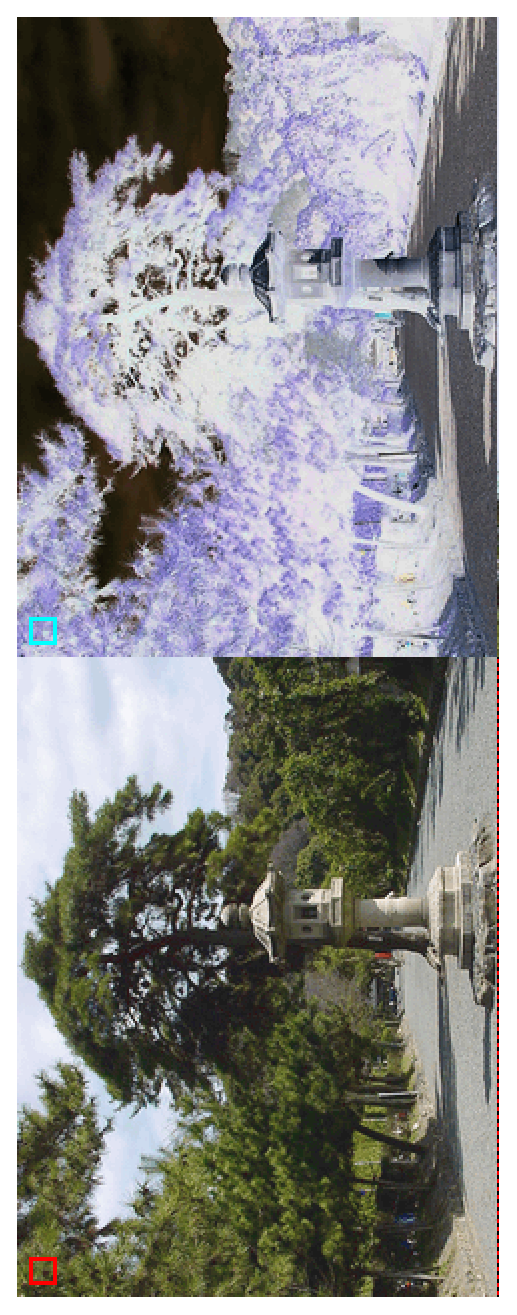
\includegraphics[angle=270,origin=b,width=0.49\textwidth]{tone_curve.eps}
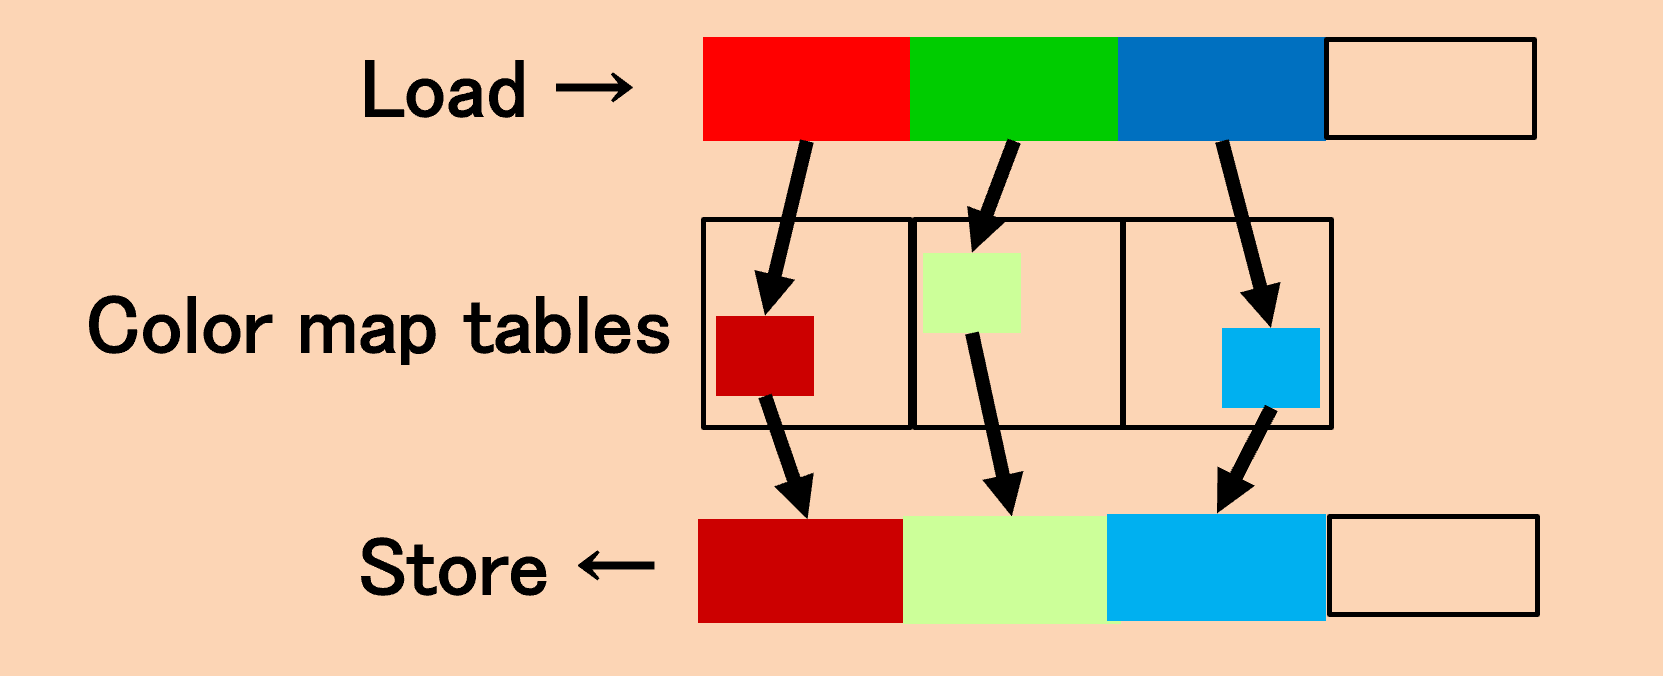
\includegraphics[angle=270,origin=b,width=0.46\textwidth]{tone1.eps}
\caption{Tone curve}
\end{figure}

\subsection{C�ˤ�륢�르�ꥺ��ε���}

\begin{screen}
\footnotesize
\begin{verbatim}
/* CPU */
for (row=0; row<HT; row++) {
  for (col=0; col<WD; col++) {
    Uint pix = hin[row*WD+col];
    hout0[row*WD+col]
      = ((ht)[pix>>24])<<24 | (ht[256+((pix>>16)&255)])<<16 | (ht[512+((pix>>8)&255)])<<8;
  }
}
\end{verbatim}
\end{screen}

\subsection{CUDA�ˤ�륢�르�ꥺ��ε���}

\begin{screen}
\scriptsize
\begin{verbatim}
/* GPU */
if (cudaSuccess != cudaMemcpy(din, hin, sizeof(Uint)*WD*HT, cudaMemcpyHostToDevice))
  { printf("can't cudaMemcpy\n"); exit(1); }
if (cudaSuccess != cudaMemcpy(dt, ht, sizeof(Uint)*256*3, cudaMemcpyHostToDevice))
  { printf("can't cudaMemcpy\n"); exit(1); }
dim3 Thread  = dim3(THREADX, THREADY, 1);
dim3 Block   = dim3(BLOCKX, BLOCKY, 1);
tone_curve<<<Block,Thread>>>(dout, din, dt); /* search triangle in {frontier,next} */
if (cudaSuccess != cudaMemcpy(hout1, dout, sizeof(Uint)*WD*HT, cudaMemcpyDeviceToHost))
  { printf("can't cudaMemcpy\n"); exit(1); }
__global__ void tone_curve(Uint *out, Uint *in, Uchar *t)
{
  int row, col;
  row = blockIdx.y*blockDim.y + threadIdx.y;
  col = blockIdx.x*blockDim.x + threadIdx.x;
  Uint pix = in[row*WD+col];
  out[row*WD+col] = ((t)[pix>>24])<<24 | (t[256+((pix>>16)&255)])<<16 | (t[512+((pix>>8)&255)])<<8;
  __syncthreads();
}
\end{verbatim}
\end{screen}

\clearpage

\subsection{IMAX����C���쵭�ҡ��襵�����룱���Ǥ���ϡ�}

\begin{screen}
\scriptsize
\begin{verbatim}
void tone_curve(r, d, t)
     unsigned int *r, *d;
     unsigned char *t;
{
  Ull  t1 = t;
  Ull  t2 = t+256;
  Ull  t3 = t+512;
  Ull  BR[16][4][4]; /* output registers in each unit */
  Ull  r0, r1, r2, r3, r4, r5, r6, r7, r8, r9, r10, r11, r12, r13, r14, r15,
       r16, r17, r18, r19, r20, r21, r22, r23, r24, r25, r26, r27, r28, r29, r30, r31;
  int loop=WD;
//EMAX5A begin tone_curve mapdist=0
  while (loop--) {
    mop(OP_LDWR,  1, &BR[0][1][1], (Ull)(r++), 0LL,         MSK_D0, (Ull)r, 320, 0,0, (Ull)NULL, 320);/* stage#0 */
    mop(OP_LDBR,  1, &BR[1][1][1], (Ull)t1,    BR[0][1][1], MSK_B3, (Ull)t1, 64, 0,0, (Ull)NULL, 64); /* stage#1 */
    mop(OP_LDBR,  1, &BR[1][2][1], (Ull)t2,    BR[0][1][1], MSK_B2, (Ull)t2, 64, 0,0, (Ull)NULL, 64); /* stage#1 */
    mop(OP_LDBR,  1, &BR[1][3][1], (Ull)t3,    BR[0][1][1], MSK_B1, (Ull)t3, 64, 0,0, (Ull)NULL, 64); /* stage#1 */
    exe(OP_MMRG, &r1, BR[1][1][1], EXP_H3210,  BR[1][2][1], EXP_H3210, BR[1][3][1], EXP_H3210, OP_NOP, 0, OP_NOP, 0);
    mop(OP_STWR,  3, &r1,          (Ull)(d++), 0LL,         MSK_D0, (Ull)d, 320, 0,0, (Ull)NULL, 320);/* stage#2 */
  }
//EMAX5A end
}
\end{verbatim}
\end{screen}

\begin{figure}[htbp]
\center
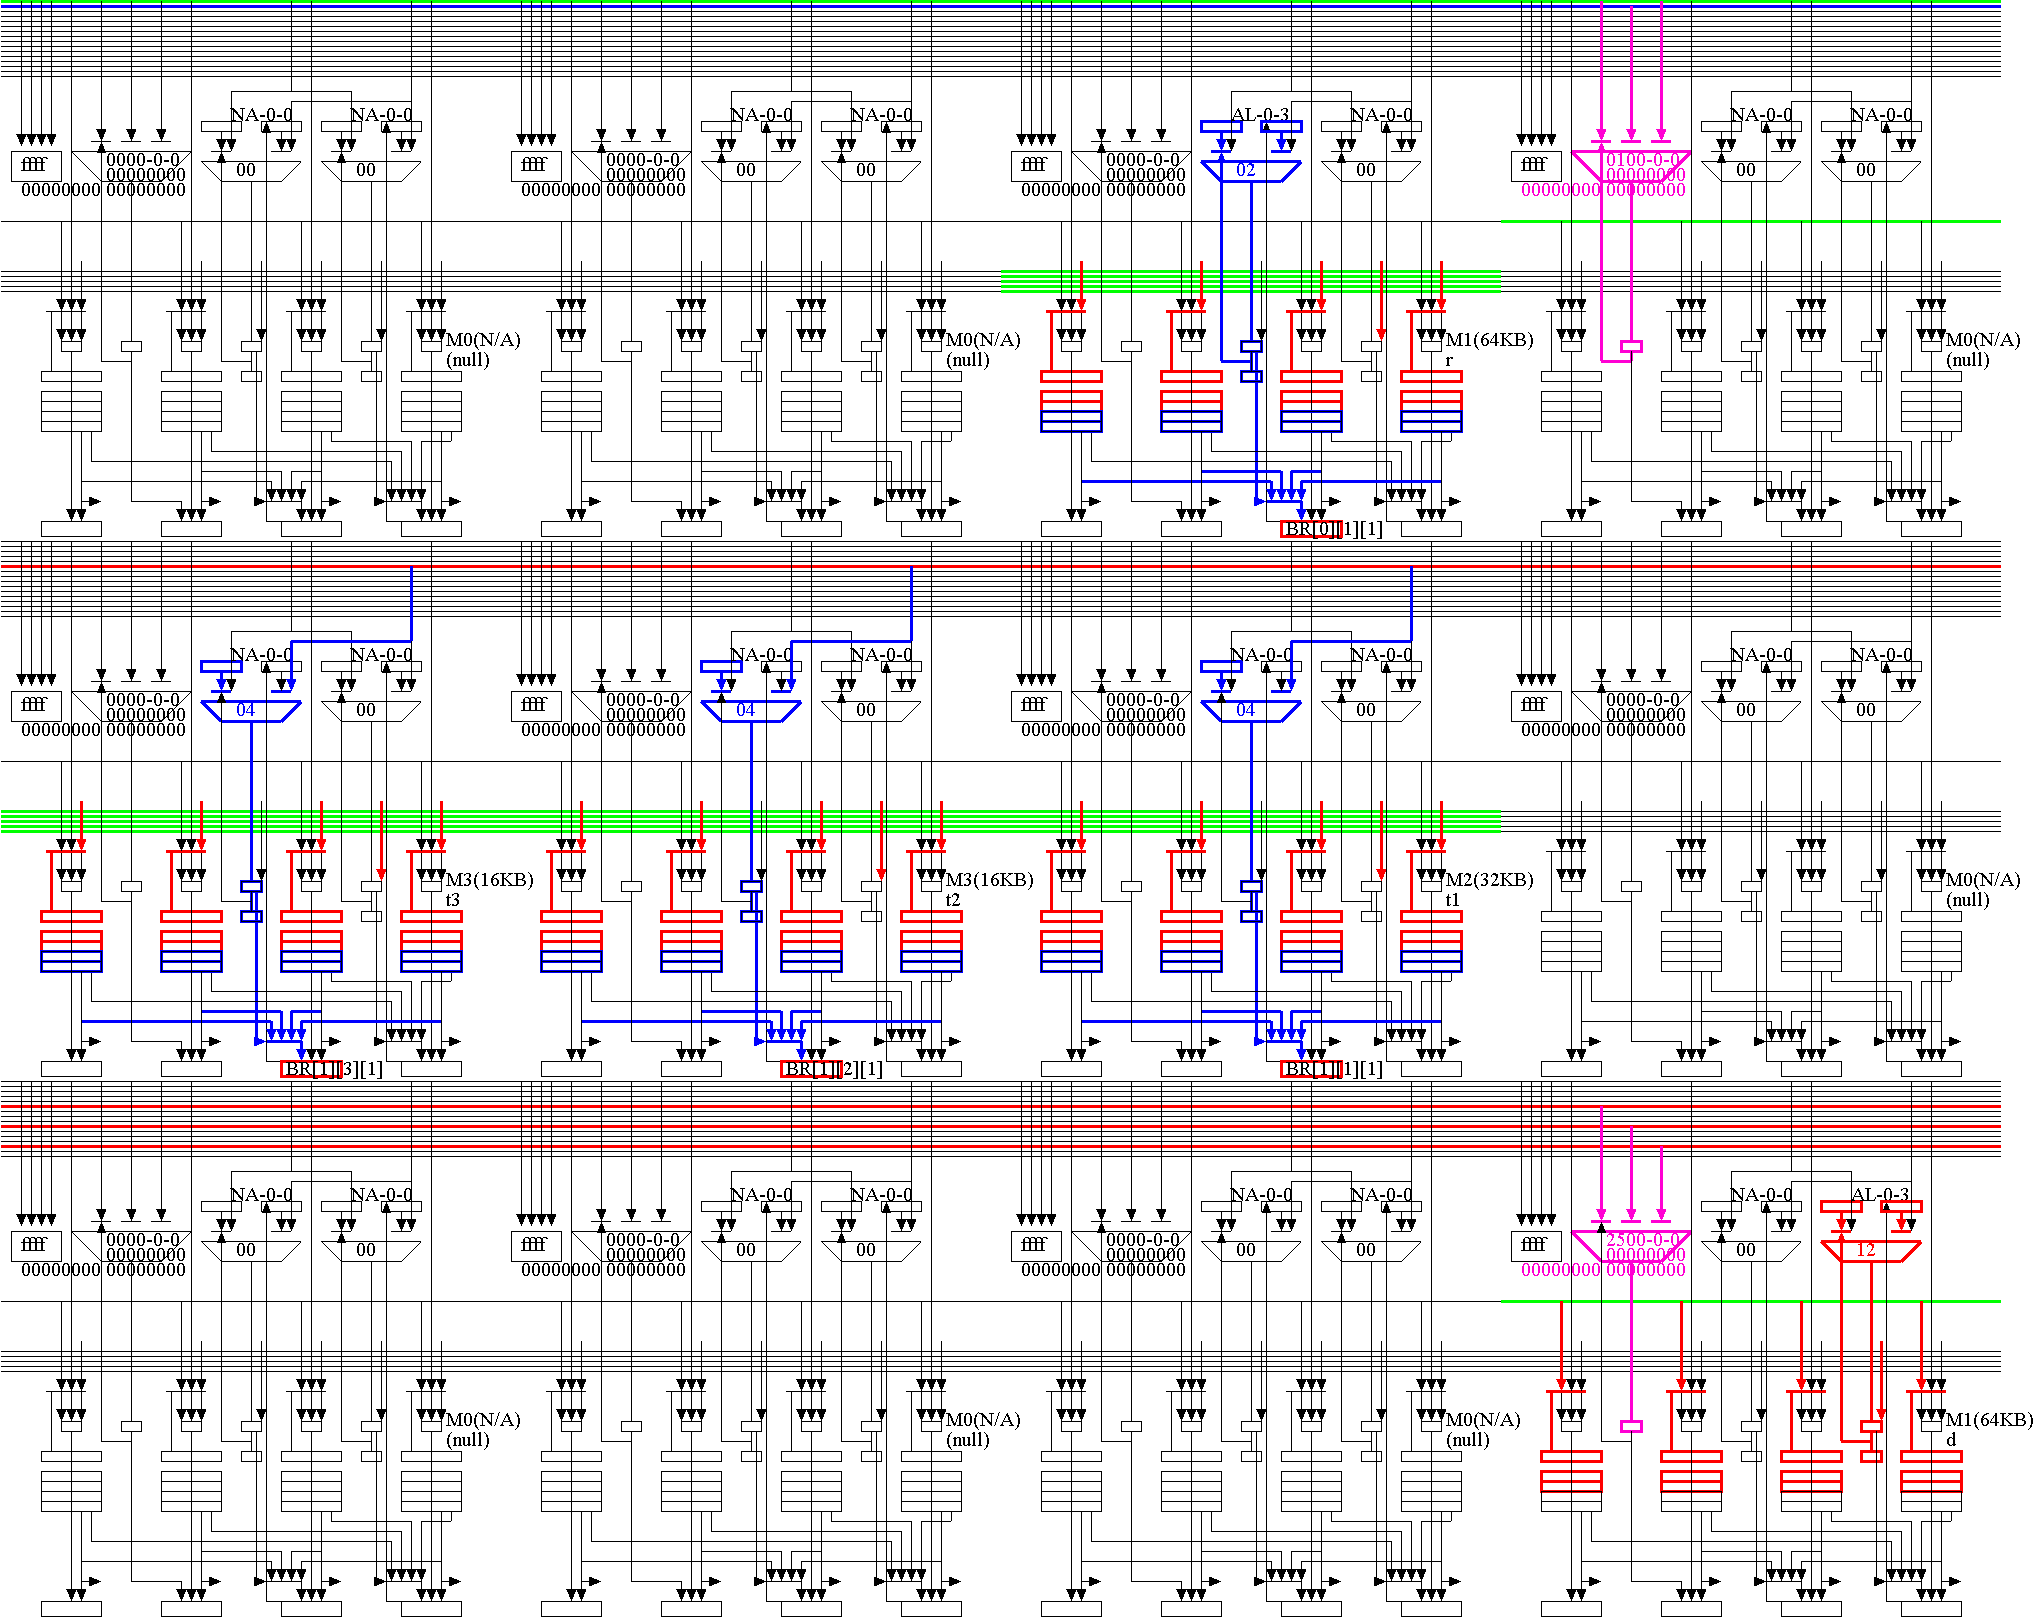
\includegraphics[angle=270,origin=b,width=0.98\textwidth]{tone3.eps}
\caption{Tone curve 1 pixel per cycle}
\end{figure}

\clearpage

\subsection{IMAX����C���쵭�ҡ��襵�����룲���Ǥ���ϡ�}

\begin{figure}[htbp]
\center
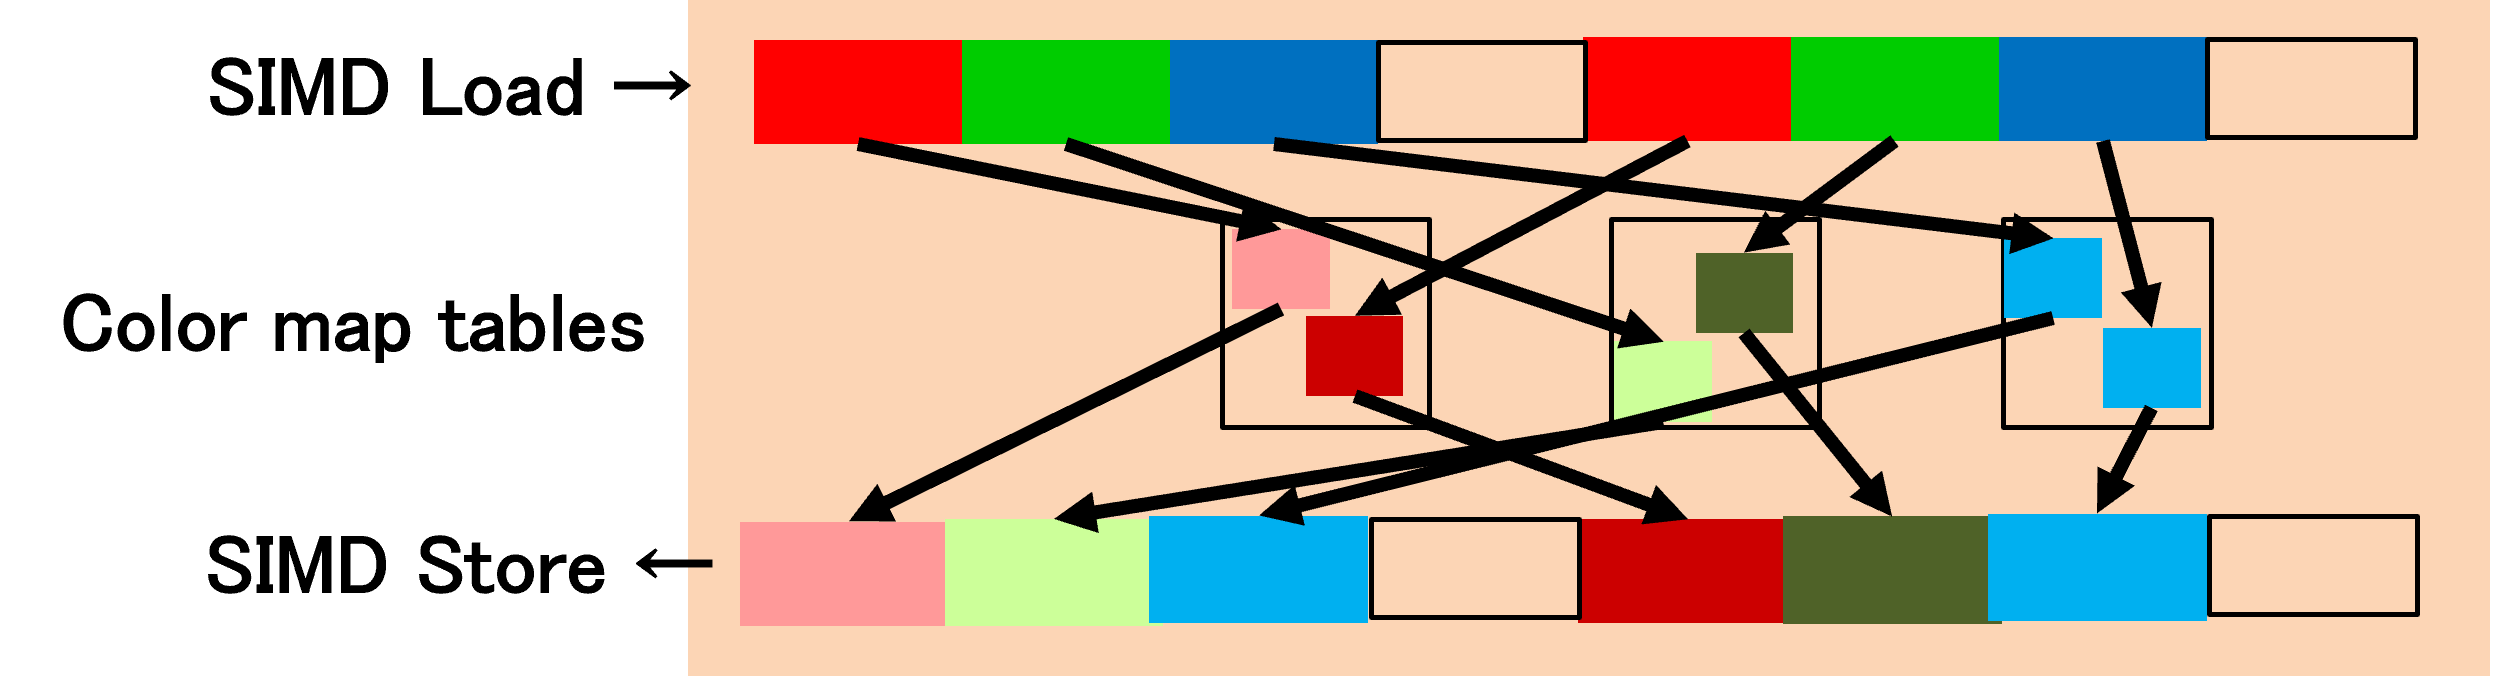
\includegraphics[angle=270,origin=b,width=0.70\textwidth]{tone2.eps}
\caption{Dual tone curve}
\end{figure}

\begin{screen}
\scriptsize
\begin{verbatim}
void tone_curve(r, d, t)
     unsigned int *r, *d;
     unsigned char *t;
{
  Ull  t1 = t;
  Ull  t2 = t+256;
  Ull  t3 = t+512;
  Ull  BR[16][4][4]; /* output registers in each unit */
  Ull  r0, r1, r2, r3, r4, r5, r6, r7, r8, r9, r10, r11, , r31;
  int loop=WD/2;
//EMAX5A begin tone_curve mapdist=0
  while (loop--) {
    mop(OP_LDR,   1, &BR[0][1][1], (Ull)(rr++), 0LL,        MSK_D0, (Ull)r, 320,  0,  0, (Ull)NULL,320);   /* stage#0 */
    mop(OP_LDBR,  1, &BR[1][1][1], (Ull)t1,    BR[0][1][1], MSK_B3, (Ull)t1, 64,  0,  0, (Ull)NULL, 64);   /* stage#1 */
    mop(OP_LDBR,  1, &BR[1][1][0], (Ull)t1,    BR[0][1][1], MSK_B7, (Ull)t1, 64,  0,  0, (Ull)NULL, 64);   /* stage#1 */
    mop(OP_LDBR,  1, &BR[1][2][1], (Ull)t2,    BR[0][1][1], MSK_B2, (Ull)t2, 64,  0,  0, (Ull)NULL, 64);   /* stage#1 */
    mop(OP_LDBR,  1, &BR[1][2][0], (Ull)t2,    BR[0][1][1], MSK_B6, (Ull)t2, 64,  0,  0, (Ull)NULL, 64);   /* stage#1 */
    mop(OP_LDBR,  1, &BR[1][3][1], (Ull)t3,    BR[0][1][1], MSK_B1, (Ull)t3, 64,  0,  0, (Ull)NULL, 64);   /* stage#1 */
    mop(OP_LDBR,  1, &BR[1][3][0], (Ull)t3,    BR[0][1][1], MSK_B5, (Ull)t3, 64,  0,  0, (Ull)NULL, 64);   /* stage#1 */
    exe(OP_CCAT,  &r1, BR[1][1][0], EXP_H3210, BR[1][1][1], EXP_H3210,        0LL, EXP_H3210, OP_NOP, 0LL, OP_NOP, 0LL);
    exe(OP_CCAT,  &r2, BR[1][2][0], EXP_H3210, BR[1][2][1], EXP_H3210,        0LL, EXP_H3210, OP_NOP, 0LL, OP_NOP, 0LL);
    exe(OP_CCAT,  &r3, BR[1][3][0], EXP_H3210, BR[1][3][1], EXP_H3210,        0LL, EXP_H3210, OP_NOP, 0LL, OP_NOP, 0LL);
    exe(OP_MMRG,  &r0,          r1, EXP_H3210, r2, EXP_H3210, r3, EXP_H3210, OP_NOP, 0LL, OP_NOP, 0LL);
    mop(OP_STR,   3, &r0,          (Ull)(dd++), 0LL,        MSK_D0, (Ull)d, 320,  0,  0, (Ull)NULL,320);   /* stage#2 */
  }
//EMAX5A end
}
\end{verbatim}
\end{screen}

\begin{figure}[htbp]
\center
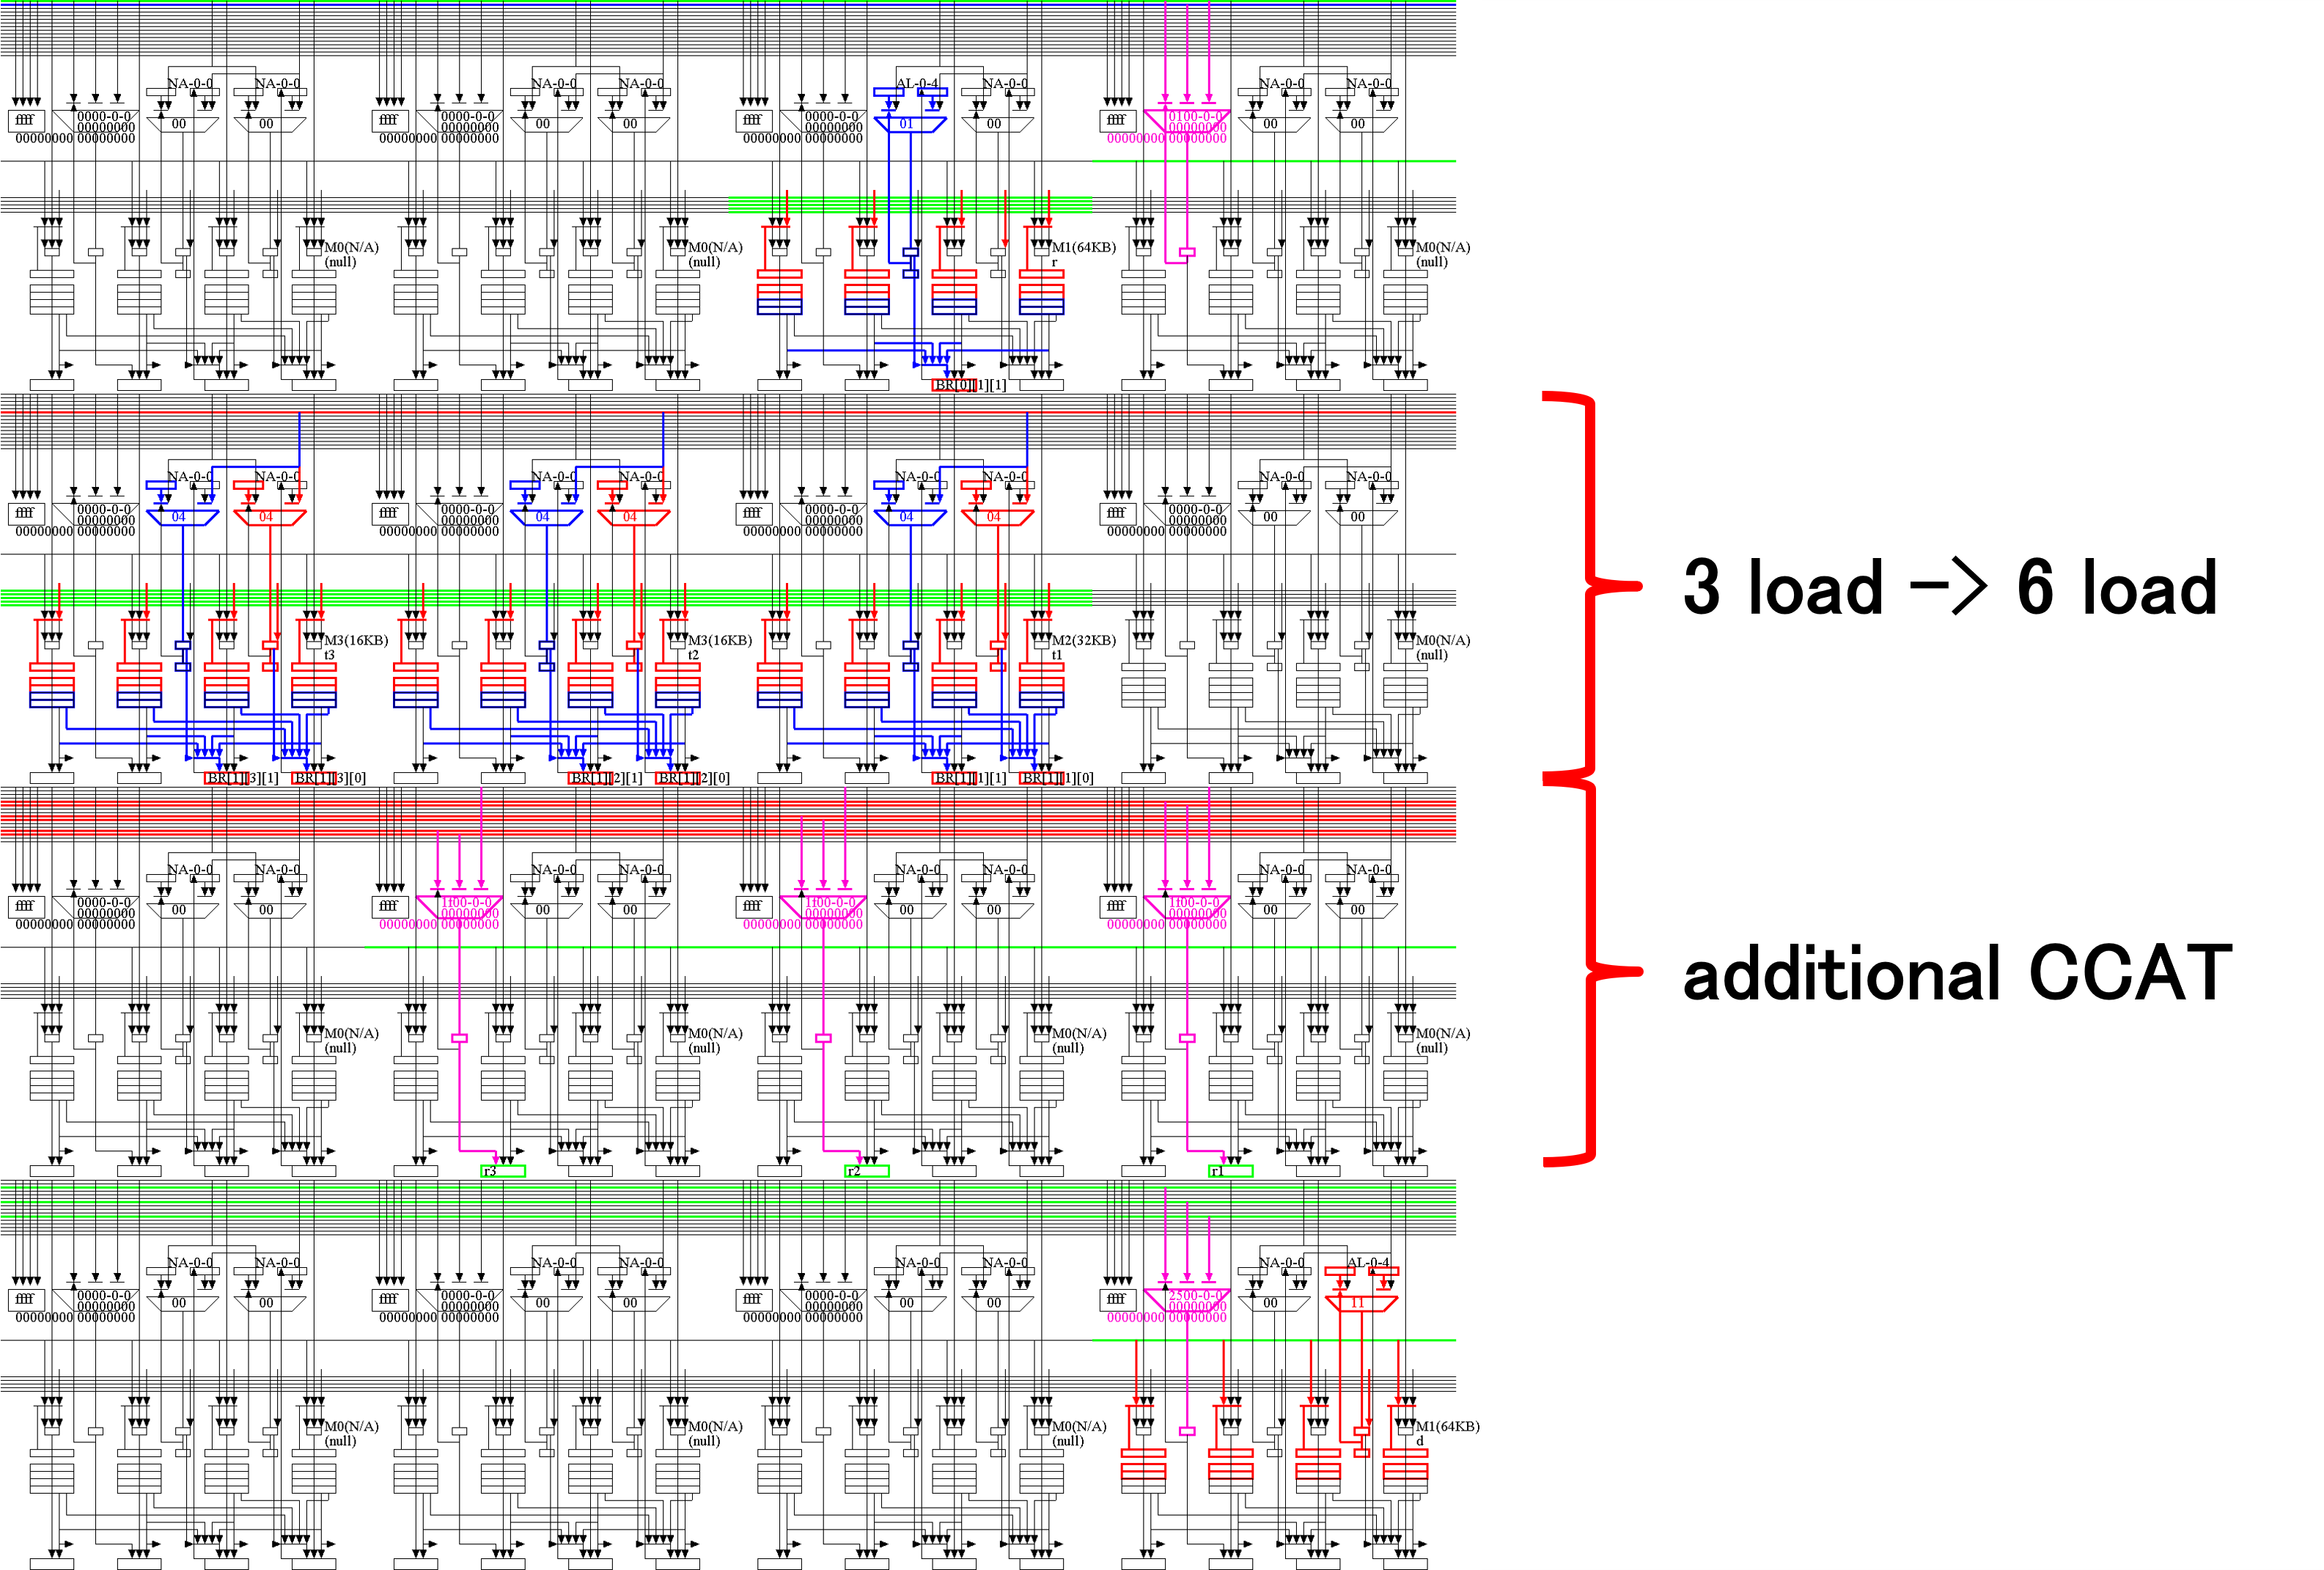
\includegraphics[angle=270,origin=b,width=0.96\textwidth]{tone4.eps}
\caption{Tone curve 2 pixels per cycle}
\end{figure}

\clearpage

\subsection{IMAX����C���쵭�ҡ�ʣ�������ѡ����ť롼�װ��¹ԡ��ޥ�����å׼¹ԡ�}

\begin{screen}
\scriptsize
\begin{verbatim}
void tone_curve(Uint *r, Uint *d, Uchar *t) /* R, D, lut */
{
#define NCHIP     1
#define RMGRP     6
#define OMAP     10
#define PAD       0
#define RRANGE   ((HT-PAD*2)/NCHIP/OMAP)
  int i;
  for(i=0; i<256; i++) {
    t[i+  0] = 0xff-i;
    t[i+256] = 0xff-i;
    t[i+512] = 0xff-i;
  }
  Ull  top, rofs, cofs, oc, pofs;
  Ull  t1 = t;
  Ull  t2 = t+256;
  Ull  t3 = t+512;
  Ull  CHIP;
  Ull  LOOP1, LOOP0;
  Ull  INIT1, INIT0;
  Ull  AR[64][4];                     /* output of EX     in each unit */
  Ull  BR[64][4][4];                  /* output registers in each unit */
  Ull  r0, r1, r2, r3, r4, r5, r6, r7, r8, r9, r10, r11, r12, r13, r14, r15;
  Ull  r16, r17, r18, r19, r20, r21, r22, r23, r24, r25, r26, r27, r28, r29, r30, r31;
  Ull  cc0, cc1, cc2, cc3, ex0, ex1;
  for (top=0; top<RRANGE; top+=RMGRP) {
    Ull  rtop0[NCHIP], dtop0[NCHIP];
    Ull  rtop1[NCHIP], dtop1[NCHIP];
    Ull  rtop2[NCHIP], dtop2[NCHIP];
    Ull  rtop3[NCHIP], dtop3[NCHIP];
    Ull  rtop4[NCHIP], dtop4[NCHIP];
    Ull  rtop5[NCHIP], dtop5[NCHIP];
    Ull  rtop6[NCHIP], dtop6[NCHIP];
    Ull  rtop7[NCHIP], dtop7[NCHIP];
    Ull  rtop8[NCHIP], dtop8[NCHIP];
    Ull  rtop9[NCHIP], dtop9[NCHIP];
    for (CHIP=0; CHIP<NCHIP; CHIP++) { /* output channels are parallelized by multi-chip (OC/#chip) */
      rtop0[CHIP] = r+(CHIP*RRANGE*OMAP+RRANGE*0+top)*WD; dtop0[CHIP] = d+(CHIP*RRANGE*OMAP+RRANGE*0+top)*WD;
      rtop1[CHIP] = r+(CHIP*RRANGE*OMAP+RRANGE*1+top)*WD; dtop1[CHIP] = d+(CHIP*RRANGE*OMAP+RRANGE*1+top)*WD;
      rtop2[CHIP] = r+(CHIP*RRANGE*OMAP+RRANGE*2+top)*WD; dtop2[CHIP] = d+(CHIP*RRANGE*OMAP+RRANGE*2+top)*WD;
      rtop3[CHIP] = r+(CHIP*RRANGE*OMAP+RRANGE*3+top)*WD; dtop3[CHIP] = d+(CHIP*RRANGE*OMAP+RRANGE*3+top)*WD;
      rtop4[CHIP] = r+(CHIP*RRANGE*OMAP+RRANGE*4+top)*WD; dtop4[CHIP] = d+(CHIP*RRANGE*OMAP+RRANGE*4+top)*WD;
      rtop5[CHIP] = r+(CHIP*RRANGE*OMAP+RRANGE*5+top)*WD; dtop5[CHIP] = d+(CHIP*RRANGE*OMAP+RRANGE*5+top)*WD;
      rtop6[CHIP] = r+(CHIP*RRANGE*OMAP+RRANGE*6+top)*WD; dtop6[CHIP] = d+(CHIP*RRANGE*OMAP+RRANGE*6+top)*WD;
      rtop7[CHIP] = r+(CHIP*RRANGE*OMAP+RRANGE*7+top)*WD; dtop7[CHIP] = d+(CHIP*RRANGE*OMAP+RRANGE*7+top)*WD;
      rtop8[CHIP] = r+(CHIP*RRANGE*OMAP+RRANGE*8+top)*WD; dtop8[CHIP] = d+(CHIP*RRANGE*OMAP+RRANGE*8+top)*WD;
      rtop9[CHIP] = r+(CHIP*RRANGE*OMAP+RRANGE*9+top)*WD; dtop9[CHIP] = d+(CHIP*RRANGE*OMAP+RRANGE*9+top)*WD;
    }
//EMAX5A begin tone_curve mapdist=0
    for (CHIP=0; CHIP<NCHIP; CHIP++) { /* output channels are parallelized by multi-chip (OC/#chip) */
/*2*/for (INIT1=1,LOOP1=RMGRP,rofs=0-WD*4; LOOP1--; INIT1=0) {     /* stage#0 *//* mapped to FOR() on BR[63][1][0] */
 /*1*/for (INIT0=1,LOOP0=WD,cofs=0-4; LOOP0--; INIT0=0) {          /* stage#0 *//* mapped to FOR() on BR[63][0][0] */
       exe(OP_ADD,  &cofs, INIT0?cofs:cofs, EXP_H3210, 4, EXP_H3210, 0,EXP_H3210,OP_AND,0x0ffffffffLL,OP_NOP,0);/* s#0*/
       exe(OP_ADD,  &rofs, rofs, EXP_H3210, INIT0?WD*4:0, EXP_H3210, 0,EXP_H3210,OP_NOP,0, OP_NOP, 0);          /* s#0*/
       exe(OP_ADD,  &pofs, rofs, EXP_H3210, cofs, EXP_H3210, 0,EXP_H3210, OP_AND,0x000000ffffffffLL, OP_NOP, 0);/* s#1*/
       /*map0*/
       mop(OP_LDWR, 1, &BR[2][1][1], rtop0[CHIP], pofs,  MSK_D0, rtop0[CHIP], WD*RMGRP,0,0,NULL,WD*RMGRP);      /* s#2*/
       mop(OP_LDBR, 1, &BR[3][1][1], t1,    BR[2][1][1], MSK_B3, t1, 256/4,  0,  0, NULL, 256/4);               /* s#3*/
       mop(OP_LDBR, 1, &BR[3][2][1], t2,    BR[2][1][1], MSK_B2, t2, 256/4,  0,  0, NULL, 256/4);               /* s#3*/
       mop(OP_LDBR, 1, &BR[3][3][1], t3,    BR[2][1][1], MSK_B1, t3, 256/4,  0,  0, NULL, 256/4);               /* s#3*/
       exe(OP_MMRG, &r1,BR[3][1][1], EXP_H3210, BR[3][2][1],EXP_H3210, BR[3][3][1],EXP_H3210,OP_NOP,0,OP_NOP,0);/* s#3*/
       mop(OP_STWR, 3, &r1,          dtop0[CHIP], pofs,  MSK_D0, dtop0[CHIP], WD*RMGRP,0,0,NULL,WD*RMGRP);      /* s#3*/
         :
       /*map9*/
       mop(OP_LDWR, 1, &BR[20][1][1],rtop9[CHIP], pofs,  MSK_D0, rtop9[CHIP], WD*RMGRP,0,0,NULL,WD*RMGRP);      /*s#20*/
       mop(OP_LDBR, 1, &BR[21][1][1],t1,    BR[20][1][1],MSK_B3, t1, 256/4,  0,  0, NULL, 256/4);               /*s#21*/
       mop(OP_LDBR, 1, &BR[21][2][1],t2,    BR[20][1][1],MSK_B2, t2, 256/4,  0,  0, NULL, 256/4);               /*s#21*/
       mop(OP_LDBR, 1, &BR[21][3][1],t3,    BR[20][1][1],MSK_B1, t3, 256/4,  0,  0, NULL, 256/4);               /*s#21*/
       exe(OP_MMRG, &r1,BR[21][1][1],EXP_H3210,BR[21][2][1],EXP_H3210,BR[21][3][1],EXP_H3210,OP_NOP,0,OP_NOP,0);/*s#21*/
       mop(OP_STWR, 3, &r1,          dtop9[CHIP], pofs,  MSK_D0, dtop9[CHIP], WD*RMGRP,0,0,NULL,WD*RMGRP);      /*s#21*/
      }
     }
    }
//EMAX5A end
  }
//EMAX5A drain_dirty_lmm
}
\end{verbatim}
\end{screen}

\clearpage

\section{Basics}

\subsection{FFT}

\shabox{
\leftline{cent\% make -f Makefile-csim.emax6+dma all clean}
\leftline{cent\% ../../src/csim/csim -x fft-csim.emax6+dma 4 4096}
}

\shabox{
\leftline{zynq\% make -f Makefile-zynq.emax6+dma all clean}
\leftline{zynq\% ./fft-zynq.emax6+dma 4 4096}
}

\subsubsection{Simple implementation}

����8192��LMM=8K*4byte*2=64KB�����Ǥ�FFT���ʤ���IMAX�ζ�������Ÿ������С�
�����̡���®����ǽ��

\begin{screen}
\tiny
\begin{verbatim}
printf("<<<ORIG>>>\n");
reset_nanosec();
BlockEnd = 1;
for (BlockSize=2; BlockSize<=NumSamples; BlockSize<<=1) {
  for (i=0; i<NumSamples; i+=BlockSize) {
    for (j=i,n=0; n<BlockEnd; j++,n++) {
      k   = j + BlockEnd;
      idx = n + BlockEnd;
      tr = art[idx]*RealOut[k] - ait[idx]*ImagOut[k];
      ti = art[idx]*ImagOut[k] + ait[idx]*RealOut[k];
      RealOut[k] = RealOut[j] - tr;
      ImagOut[k] = ImagOut[j] - ti;
      RealOut[j] += tr;
      ImagOut[j] += ti;
  } }
  BlockEnd = BlockSize;
}
\end{verbatim}
\end{screen}

\begin{screen}
\tiny
\begin{verbatim}
  Ull  CHIP;
  Ull  LOOP1, LOOP0;
  Ull  INIT1, INIT0;
  Ull  AR[64][4];                     /* output of EX     in each unit */
  Ull  BR[64][4][4];                  /* output registers in each unit */
  Ull  r0, r1, r2, r3, r4, r5, r6, r7, r8, r9, r10, r11, r12, r13, r14, r15;
  Ull  r16, r17, r18, r19, r20, r21, r22, r23, r24, r25, r26, r27, r28, r29, r30, r31;
  Ull  cc0, cc1, cc2, cc3, ex0, ex1;
  Ull  ar, ai, rok, iok, roj, ioj;
  Ull  tr0, ti0, tr1, ti1, roj1, ioj1;

  printf("<<<IMAX>>> NumSamples=%d (LMM should be >= %dB)\n", NumSamples, NumSamples*4*2);
  reset_nanosec();

#define fft_core0(r) \
          exe(OP_ADD,     &j,         i,        EXP_H3210,  n,       EXP_H3210, 0LL,          EXP_H3210, OP_NOP, 0LL, OP_SLL, 2LL); /* stage#1 */\
          exe(OP_ADD3,    &k,         i,        EXP_H3210,  n,       EXP_H3210, BlockEnd,     EXP_H3210, OP_NOP, 0LL, OP_SLL, 2LL); /* stage#1 */\
          exe(OP_ADD3,    &idx,       0LL,      EXP_H3210,  n,       EXP_H3210, BlockEnd,     EXP_H3210, OP_NOP, 0LL, OP_SLL, 2LL); /* stage#1 */\
          exe(OP_NOP,     &AR[r][0],  0LL,      EXP_H3210,  0LL,     EXP_H3210, 0LL,          EXP_H3210, OP_NOP, 0LL, OP_NOP, 0LL); /* stage#2 [2][0]     */\
          mop(OP_LDWR, 3, &rok,       RealOut,  k,          MSK_D0,  RealOut,   NumSamples,   0, 1,  NULL,  NumSamples);            /* stage#2 RealOut[k] */\
          mop(OP_LDWR, 3, &roj,       j,        RealOut,    MSK_D0,  RealOut,   NumSamples,   0, 1,  NULL,  NumSamples);            /* stage#2 RealOut[j] */\
          exe(OP_NOP,     &AR[r][2],  0LL,      EXP_H3210,  0LL,     EXP_H3210, 0LL,          EXP_H3210, OP_NOP, 0LL, OP_NOP, 0LL); /* stage#2 [2][2]     */\
          mop(OP_LDWR, 3, &iok,       ImagOut,  k,          MSK_D0,  ImagOut,   NumSamples,   0, 1,  NULL,  NumSamples);            /* stage#2 ImagOut[k] */\
          mop(OP_LDWR, 3, &ioj,       j,        ImagOut,    MSK_D0,  ImagOut,   NumSamples,   0, 1,  NULL,  NumSamples)             /* stage#2 ImagOut[j] */
#define fft_core1(r) \
          exe(OP_NOP,     &AR[r][0],  0LL,      EXP_H3210,  0LL,     EXP_H3210, 0LL,          EXP_H3210, OP_NOP, 0LL, OP_NOP, 0LL); /* stage#3 [3][0]     */\
          mop(OP_LDWR, 3, &ar,        art,      idx,        MSK_D0,  art,       NumSamples,   0, 0,  NULL,  NumSamples);            /* stage#3 art[idx]   */\
          exe(OP_NOP,     &AR[r][2],  0LL,      EXP_H3210,  0LL,     EXP_H3210, 0LL,          EXP_H3210, OP_NOP, 0LL, OP_NOP, 0LL); /* stage#3 [3][2]     */\
          mop(OP_LDWR, 3, &ai,        ait,      idx,        MSK_D0,  ait,       NumSamples,   0, 0,  NULL,  NumSamples);            /* stage#3 ait[idx]   */\
          exe(OP_FML,     &tr0,       ar,       EXP_H3210,  rok,     EXP_H3210, 0LL,          EXP_H3210, OP_NOP, 0LL, OP_NOP, 0LL); /* stage#4 */\
          exe(OP_FML,     &ti0,       ar,       EXP_H3210,  iok,     EXP_H3210, 0LL,          EXP_H3210, OP_NOP, 0LL, OP_NOP, 0LL); /* stage#4 */\
          exe(OP_FMS,     &tr1,       tr0,      EXP_H3210,  ai,      EXP_H3210, iok,          EXP_H3210, OP_NOP, 0LL, OP_NOP, 0LL); /* stage#5 */\
          exe(OP_FMA,     &ti1,       ti0,      EXP_H3210,  ai,      EXP_H3210, rok,          EXP_H3210, OP_NOP, 0LL, OP_NOP, 0LL)  /* stage#5 */
#define fft_final(r) \
          exe(OP_FMS,     &AR[r][0],  roj,      EXP_H3210,  tr1,     EXP_H3210, 0x3f800000LL, EXP_H3210, OP_NOP, 0LL, OP_NOP, 0LL); /* stage#6 */\
          mop(OP_STWR, 3, &AR[r][0],  RealOut,  k,          MSK_D0,  RealOut,   NumSamples,   0, 0,  NULL,  NumSamples);            /* stage#6 */\
          exe(OP_FAD,     &AR[r][1],  roj,      EXP_H3210,  tr1,     EXP_H3210, 0LL,          EXP_H3210, OP_NOP, 0LL, OP_NOP, 0LL); /* stage#6 */\
          mop(OP_STWR, 3, &AR[r][1],  RealOut,  j,          MSK_D0,  RealOut,   NumSamples,   0, 0,  NULL,  NumSamples);            /* stage#6 */\
          exe(OP_FMS,     &AR[r][2],  ioj,      EXP_H3210,  ti1,     EXP_H3210, 0x3f800000LL, EXP_H3210, OP_NOP, 0LL, OP_NOP, 0LL); /* stage#6 */\
          mop(OP_STWR, 3, &AR[r][2],  ImagOut,  k,          MSK_D0,  ImagOut,   NumSamples,   0, 0,  NULL,  NumSamples);            /* stage#6 */\
          exe(OP_FAD,     &AR[r][3],  ioj,      EXP_H3210,  ti1,     EXP_H3210, 0LL,          EXP_H3210, OP_NOP, 0LL, OP_NOP, 0LL); /* stage#6 */\
          mop(OP_STWR, 3, &AR[r][3],  ImagOut,  j,          MSK_D0,  ImagOut,   NumSamples,   0, 0,  NULL,  NumSamples)             /* stage#6 */
  BlockEnd = 1;
  for (BlockSize=2; BlockSize<=NumSamples; BlockSize<<=1) {
//with-prefetch/post-drain
//EMAX5A begin imax mapdist=0
/*3*/for (CHIP=0; CHIP<NCHIP; CHIP++) {
  /*2*/for (INIT1=1,LOOP1=NumSamples/BlockSize,i=0LL<<32|(0-BlockSize)&0xffffffff; LOOP1--; INIT1=0) {
    /*1*/for (INIT0=1,LOOP0=BlockEnd,n=0LL<<32|(0-1LL)&0xffffffff; LOOP0--; INIT0=0) {
          exe(OP_ADD,     &i,     i,         EXP_H3210,   INIT0?BlockSize:0, EXP_H3210, 0LL, EXP_H3210, OP_NOP, 0LL, OP_NOP, 0LL);          /* stage#0 */
          exe(OP_ADD,     &n,     INIT0?n:n, EXP_H3210,   0LL<<32|1LL,       EXP_H3210, 0LL,          EXP_H3210, OP_NOP, 0LL, OP_NOP, 0LL); /* stage#0 */
          fft_core0(2); /* stage#2   */
          fft_core1(3); /* stage#3-5 */
          fft_final(6); /* stage#6   */
    } } }
//EMAX5A end
//EMAX5A drain_dirty_lmm
    BlockEnd = BlockSize;
  }
\end{verbatim}
\end{screen}

\begin{figure}[htbp]
\center
\epsfile{file=fourierf-imax-emax6.eps,width=1.00\textwidth}
\caption{FFT}
\end{figure}

\clearpage

\subsubsection{Pipelined implementation}

FFT�Υѥ��ץ饤���ǡ�����4096��LMM=4K*4byte*2*2=64KB�����Ǥ�FFT����֤�LMM��
���֥�Хåե��Ȥ��ƻ��Ѥ��Ƥ��롥

\begin{screen}
\tiny
\begin{verbatim}
  Ull  CHIP;
  Ull  LOOP1, LOOP0, L;
  Ull  INIT1, INIT0;
  Ull  AR[64][4];                     /* output of EX     in each unit */
  Ull  BR[64][4][4];                  /* output registers in each unit */
  Ull  r0, r1, r2, r3, r4, r5, r6, r7, r8, r9, r10, r11, r12, r13, r14, r15;
  Ull  r16, r17, r18, r19, r20, r21, r22, r23, r24, r25, r26, r27, r28, r29, r30, r31;
  Ull  cc0, cc1, cc2, cc3, ex0, ex1;
  Ull  J[16], K[16], IDX[16]; /* log2(NumSamples=65536)=16�ޤ��б��� */
  Ull  BufReal[16], BufImag[16];
  Ull  ar, ai, rok, iok, roj, ioj, tr0, ti0, tr1, ti1;
  Ull  Pipeline, Lmmrotate; /* log2(NumSamples=65536)=16�󷫤��֤���,�ǽ��ʤ�LMM��,�ǽ��RealOut/ImagOut����Ǽ����� */
  printf("<<<IMAX>>> NumSamples=%d (LMM should be >= %dB)\n", NumSamples, NumSamples*4*2);
  reset_nanosec();
#define fft_core0(r, x, MASK_M, MASK_N, BS) \
        exe(OP_ADD,     &i,         L,          EXP_H3210,  L,       EXP_H3210, 0LL,          EXP_H3210, OP_AND, MASK_M, OP_NOP, 0LL); /* stage#1 i  =(L*2)&M   */\
        exe(OP_ADD,     &n,         L,          EXP_H3210,  0LL,     EXP_H3210, 0LL,          EXP_H3210, OP_AND, MASK_N, OP_NOP, 0LL); /* stage#1 n  =L    &N   */\
        exe(OP_ADD,     &J[x],      i,          EXP_H3210,  n,       EXP_H3210, 0LL,          EXP_H3210, OP_NOP, 0LL,    OP_SLL, 2LL); /* stage#2 j  =i+n       */\
        exe(OP_ADD3,    &K[x],      i,          EXP_H3210,  n,       EXP_H3210, BS,           EXP_H3210, OP_NOP, 0LL,    OP_SLL, 2LL); /* stage#2 k  =i+n+BS(2) */\
        exe(OP_ADD3,    &IDX[x],    0LL,        EXP_H3210,  n,       EXP_H3210, BS,           EXP_H3210, OP_NOP, 0LL,    OP_SLL, 2LL)  /* stage#2 idx=  n+BS(2) */
#define fft_core1(r, x) \
        exe(OP_NOP,     &AR[r][0],  0LL,        EXP_H3210,  0LL,     EXP_H3210, 0LL,          EXP_H3210, OP_NOP, 0LL,    OP_NOP, 0LL); /* stage#3 [3][0]        */\
        mop(OP_LDWR, 3, &rok,       RealIn,     K[x],       MSK_D0,  RealIn,    NumSamples,   0, 1,  NULL,  NumSamples);               /* stage#3 RealIn[k]     */\
        mop(OP_LDWR, 3, &roj,       J[x],       RealIn,     MSK_D0,  RealIn,    NumSamples,   0, 1,  NULL,  NumSamples);               /* stage#3 RealIn[j]     */\
        exe(OP_NOP,     &AR[r][2],  0LL,        EXP_H3210,  0LL,     EXP_H3210, 0LL,          EXP_H3210, OP_NOP, 0LL,    OP_NOP, 0LL); /* stage#3 [3][2]        */\
        mop(OP_LDWR, 3, &iok,       ImagIn,     K[x],       MSK_D0,  ImagIn,    NumSamples,   0, 1,  NULL,  NumSamples);               /* stage#3 ImagIn[k]     */\
        mop(OP_LDWR, 3, &ioj,       J[x],       ImagIn,     MSK_D0,  ImagIn,    NumSamples,   0, 1,  NULL,  NumSamples)                /* stage#3 ImagIn[j]     */
#define fft_core2(r, x, y, MASK_M, MASK_N, BS) \
        exe(OP_NOP,     &AR[r][0],  0LL,        EXP_H3210,  0LL,     EXP_H3210, 0LL,          EXP_H3210, OP_NOP, 0LL,    OP_NOP, 0LL); /* stage#4 [4][0]        */\
        exe(OP_ADD,     &i,         L,          EXP_H3210,  L,       EXP_H3210, 0LL,          EXP_H3210, OP_AND, MASK_M, OP_NOP, 0LL); /* stage#4 i  =(L*2)&M   */\
        mop(OP_LDWR, 3, &ar,        art,        IDX[x],     MSK_D0,  art,       NumSamples,   0, 0,  NULL,  NumSamples);               /* stage#4 art[idx]      */\
        exe(OP_NOP,     &AR[r][2],  0LL,        EXP_H3210,  0LL,     EXP_H3210, 0LL,          EXP_H3210, OP_NOP, 0LL,    OP_NOP, 0LL); /* stage#4 [4][2]        */\
        exe(OP_ADD,     &n,         L,          EXP_H3210,  0LL,     EXP_H3210, 0LL,          EXP_H3210, OP_AND, MASK_N, OP_NOP, 0LL); /* stage#4 n  = L   &N   */\
        mop(OP_LDWR, 3, &ai,        ait,        IDX[x],     MSK_D0,  ait,       NumSamples,   0, 0,  NULL,  NumSamples);               /* stage#4 ait[idx]      */\
        \
        exe(OP_ADD,     &J[y],      i,          EXP_H3210,  n,       EXP_H3210, 0LL,          EXP_H3210, OP_NOP, 0LL,    OP_SLL, 2LL); /* stage#5 j  =i+n       */\
        exe(OP_ADD3,    &K[y],      i,          EXP_H3210,  n,       EXP_H3210, BS,           EXP_H3210, OP_NOP, 0LL,    OP_SLL, 2LL); /* stage#5 k  =i+n+BS(2) */\
        exe(OP_FML,     &tr0,       ar,         EXP_H3210,  rok,     EXP_H3210, 0LL,          EXP_H3210, OP_NOP, 0LL,    OP_NOP, 0LL); /* stage#5 */\
        exe(OP_FML,     &ti0,       ar,         EXP_H3210,  iok,     EXP_H3210, 0LL,          EXP_H3210, OP_NOP, 0LL,    OP_NOP, 0LL); /* stage#5 */\
        \
        exe(OP_ADD3,    &IDX[y],    0LL,        EXP_H3210,  n,       EXP_H3210, BS,           EXP_H3210, OP_NOP, 0LL,    OP_SLL, 2LL); /* stage#6 idx=  n+BS(2) */\
        exe(OP_FMS,     &tr1,       tr0,        EXP_H3210,  ai,      EXP_H3210, iok,          EXP_H3210, OP_NOP, 0LL,    OP_NOP, 0LL); /* stage#6 */\
        exe(OP_FMA,     &ti1,       ti0,        EXP_H3210,  ai,      EXP_H3210, rok,          EXP_H3210, OP_NOP, 0LL,    OP_NOP, 0LL)  /* stage#6 */
#define fft_core3(r, x, y) \
        exe(OP_FMS,     &AR[r][0],  roj,        EXP_H3210,  tr1,     EXP_H3210, 0x3f800000LL, EXP_H3210, OP_NOP, 0LL,    OP_NOP, 0LL); /* stage#7 */\
        mop(OP_STWR, 3, &AR[r][0],  BufReal[x], K[x],       MSK_D0,  BufReal[x],0LL,          0, 0,  NULL,  0LL);                      /* stage#7 */\
        mop(OP_LDWR, 3, &rok,       K[y],       BufReal[y], MSK_D0,  BufReal[x],0LL,          0, 0,  NULL,  0LL);                      /* stage#7 BufReal[k] */\
        exe(OP_FAD,     &AR[r][1],  roj,        EXP_H3210,  tr1,     EXP_H3210, 0LL,          EXP_H3210, OP_NOP, 0LL,    OP_NOP, 0LL); /* stage#7 */\
        mop(OP_STWR, 3, &AR[r][1],  BufReal[x], J[x],       MSK_D0,  BufReal[x],0LL,          0, 0,  NULL,  0LL);                      /* stage#7 */\
        mop(OP_LDWR, 3, &roj,       J[y],       BufReal[y], MSK_D0,  BufReal[x],0LL,          0, 0,  NULL,  0LL);                      /* stage#7 BufReal[j] */\
        exe(OP_FMS,     &AR[r][2],  ioj,        EXP_H3210,  ti1,     EXP_H3210, 0x3f800000LL, EXP_H3210, OP_NOP, 0LL,    OP_NOP, 0LL); /* stage#7 */\
        mop(OP_STWR, 3, &AR[r][2],  BufImag[x], K[x],       MSK_D0,  BufImag[x],0LL,          0, 0,  NULL,  0LL);                      /* stage#7 */\
        mop(OP_LDWR, 3, &iok,       K[y],       BufImag[y], MSK_D0,  BufImag[x],0LL,          0, 0,  NULL,  0LL);                      /* stage#7 BufImag[k] */\
        exe(OP_FAD,     &AR[r][3],  ioj,        EXP_H3210,  ti1,     EXP_H3210, 0LL,          EXP_H3210, OP_NOP, 0LL,    OP_NOP, 0LL); /* stage#7 */\
        mop(OP_STWR, 3, &AR[r][3],  BufImag[x], J[x],       MSK_D0,  BufImag[x],0LL,          0, 0,  NULL,  0LL);                      /* stage#7 */\
        mop(OP_LDWR, 3, &ioj,       J[y],       BufImag[y], MSK_D0,  BufImag[x],0LL,          0, 0,  NULL,  0LL)                       /* stage#7 BufImag[j] */
#define fft_final(r, x) \
        exe(OP_FMS,     &AR[r][0],  roj,        EXP_H3210,  tr1,     EXP_H3210, 0x3f800000LL, EXP_H3210, OP_NOP, 0LL,    OP_NOP, 0LL); /* stage#7 */\
        mop(OP_STWR, 3, &AR[r][0],  RealOut,    K[x],       MSK_D0,  RealOut,   NumSamples,   0, 0,  NULL,  NumSamples);               /* stage#7 */\
        exe(OP_FAD,     &AR[r][1],  roj,        EXP_H3210,  tr1,     EXP_H3210, 0LL,          EXP_H3210, OP_NOP, 0LL,    OP_NOP, 0LL); /* stage#7 */\
        mop(OP_STWR, 3, &AR[r][1],  RealOut,    J[x],       MSK_D0,  RealOut,   NumSamples,   0, 0,  NULL,  NumSamples);               /* stage#7 */\
        exe(OP_FMS,     &AR[r][2],  ioj,        EXP_H3210,  ti1,     EXP_H3210, 0x3f800000LL, EXP_H3210, OP_NOP, 0LL,    OP_NOP, 0LL); /* stage#7 */\
        mop(OP_STWR, 3, &AR[r][2],  ImagOut,    K[x],       MSK_D0,  ImagOut,   NumSamples,   0, 0,  NULL,  NumSamples);               /* stage#7 */\
        exe(OP_FAD,     &AR[r][3],  ioj,        EXP_H3210,  ti1,     EXP_H3210, 0LL,          EXP_H3210, OP_NOP, 0LL,    OP_NOP, 0LL); /* stage#7 */\
        mop(OP_STWR, 3, &AR[r][3],  ImagOut,    J[x],       MSK_D0,  ImagOut,   NumSamples,   0, 0,  NULL,  NumSamples)                /* stage#7 */
  for (Pipeline=0; Pipeline<NumBits; Pipeline++) {
    /* 0: buf[0]=[(0+4-0)%4]:0 buf[1]=[(1+4-0)%4]:1 buf[2]=[(2+4-0)%4]:2 buf[3]=[(3+4-0)%4]:3 */
    /* 1: buf[0]=[(0+4-1)%4]:3 buf[1]=[(1+4-1)%4]:0 buf[2]=[(2+4-1)%4]:1 buf[3]=[(3+4-1)%4]:2 */
    /* 2: buf[0]=[(0+4-2)%4]:2 buf[1]=[(1+4-2)%4]:3 buf[2]=[(2+4-2)%4]:0 buf[3]=[(3+4-2)%4]:1 */
    for (Lmmrotate=0; Lmmrotate<=NumBits; Lmmrotate++) {
      BufReal[Lmmrotate] = &pseudoLMM[NumSamples*(((Lmmrotate+NumBits+1-Pipeline)%(NumBits+1))*2  )];
      BufImag[Lmmrotate] = &pseudoLMM[NumSamples*(((Lmmrotate+NumBits+1-Pipeline)%(NumBits+1))*2+1)];
    }
//EMAX5A begin pipeline mapdist=0
/*3*/for (CHIP=0; CHIP<NCHIP; CHIP++) {
 /*1*/for (INIT0=1,LOOP0=NumSamples/2,L=0LL<<32|(0-1LL)&0xffffffff; LOOP0--; INIT0=0) { /* NumSamples<=4096 */
        exe(OP_ADD,     &L,         L,          EXP_H3210,  0LL<<32|1LL, EXP_H3210, 0LL,      EXP_H3210, OP_NOP, 0LL,    OP_NOP, 0LL); /* stage#0 */
#if (H==2)
        fft_core0( 1,  0,     0xfffeLL, 0x0000LL, 1LL); /* stage#1-2   */
        fft_core1( 3,  0);                              /* stage#3     */
        fft_core2( 4,  0,  1, 0xfffcLL, 0x0001LL, 2LL); /* stage#4-6   */
        fft_final( 7,  0);                              /* stage#7     */
#endif
#if (H==4096)
        fft_core0( 1,  0,     0xfffeLL, 0x0000LL,    1LL); /* stage#1-2   */
        fft_core1( 3,  0);                                 /* stage#3     */
        fft_core2( 4,  0,  1, 0xfffcLL, 0x0001LL,    2LL); /* stage#4-6   */
        fft_core3( 7,  0,  1);                             /* stage#7     */
        fft_core2( 8,  1,  2, 0xfff8LL, 0x0003LL,    4LL); /* stage#8-10  */
        fft_core3(11,  1,  2);                             /* stage#11    */
        fft_core2(12,  2,  3, 0xfff0LL, 0x0007LL,    8LL); /* stage#12-14 */
        fft_core3(15,  2,  3);                             /* stage#15    */
        fft_core2(16,  3,  4, 0xffe0LL, 0x000fLL,   16LL); /* stage#16-18 */
        fft_core3(19,  3,  4);                             /* stage#19    */
        fft_core2(20,  4,  5, 0xffc0LL, 0x001fLL,   32LL); /* stage#20-22 */
        fft_core3(23,  4,  5);                             /* stage#23    */
        fft_core2(24,  5,  6, 0xff80LL, 0x003fLL,   64LL); /* stage#24-26 */
        fft_core3(27,  5,  6);                             /* stage#27    */
        :
        fft_core2(44, 10, 11, 0xf000LL, 0x07ffLL, 2048LL); /* stage#44-46 */
        fft_core3(47, 10, 11);                             /* stage#47    */
        fft_core2(48, 11, 12, 0xe000LL, 0x0fffLL, 4096LL); /* stage#48-50 */
        fft_final(51, 11);                                 /* stage#51    */
#endif
    } }
//EMAX5A end
//EMAX5A drain_dirty_lmm
  }
\end{verbatim}
\end{screen}

\begin{figure}[htbp]
\center
\epsfile{file=fourierf-pipeline-emax6.eps,width=1.00\textwidth}
\caption{FFT}
\end{figure}

\clearpage

\subsection{Merge sort}

\shabox{
\leftline{cent\% make -f Makefile-csim.emax6+dma all clean}
\leftline{cent\% ../../src/csim/csim -x sort-merge-csim.emax6+dma 4096}
}

\shabox{
\leftline{zynq\% make -f Makefile-zynq.emax6+dma all clean}
\leftline{zynq\% ./sort-merge-zynq.emax6+dma 4096}
}

\vskip .1in

����4096��LMM=4K*8byte*2=64KB�����ǤΥѥ��ץ饤����merge sort����֤�LMM���
�֥�Хåե��Ȥ��ƻ��Ѥ��Ƥ��롥�ʤ������ϥǡ����ϳ�����8�Х��ȤǤ��롥���4
�Х��Ȥ��羮����оݡ�����4�Х��Ȥϥݥ��󥿤�°���ʤ�Ǥ�դ��ͤ˻��ѤǤ��롥

\begin{screen}
\tiny
\begin{verbatim}
printf("<<<ORIG>>>\n");
BlockEnd = 1;
for (BlockSize=2; BlockSize<=NumSamples; BlockSize<<=1) {
  for (i=0; i<NumSamples; i+=BlockSize) {
    for (j=i,k=i+BlockEnd,t=i; t<i+BlockSize; t++) {
      int cc0 = j<i+BlockEnd;
      int cc1 = k<i+BlockSize;
      int cc2 = In[j].val < In[k].val;
      if ((( cc2 && cc1) || !cc1) && cc0) /* 7,5,1 0x00a2 */ Out[t] = In[j++];
      if (((!cc2 && cc0) || !cc0) && cc1) /* 6,3,2 0x004c */ Out[t] = In[k++];
  } }
  BlockEnd = BlockSize;
  for (i=0; i<NumSamples; i++)
    In[i] = Out[i];
}
\end{verbatim}
\end{screen}

\begin{screen}
\tiny
\begin{verbatim}
#define NCHIP 1
#define H     4096
Ull  CHIP;
Ull  LOOP1, LOOP0, L8;
Ull  INIT1, INIT0;
Ull  AR[64][4];           /* output of EX     in each unit */
Ull  BR[64][4][4];        /* output registers in each unit */
Ull  r0, r1, r2, r3, r4, r5, r6, r7, r8, r9, r10, r11, r12, r13, r14, r15;
Ull  r16, r17, r18, r19, r20, r21, r22, r23, r24, r25, r26, r27, r28, r29, r30, r31;
Ull  cc0, cc1, cc2, cc3, ex0, ex1, ex2, ex3;
Ull  Buf[32];
Ull  base, J[16], K[16];  /* log2(NumSamples=65536)=16�ޤ��б��� */
Ull  Pipeline, Lmmrotate; /* log2(NumSamples=65536)=16�󷫤��֤���,�ǽ��ʤ�LMM��,�ǽ��Out����Ǽ����� */
printf("<<<IMAX>>> NumSamples=%d (LMM should be >= %dB)\n", NumSamples, NumSamples2*4);

for (i=0; i<NumBits; i++) { J[i]=0; K[i]=0; }
#define sort_core0(r, rp1, x, MASK_M, In, BE8) \
 exe(OP_NOP,      &AR[r][1],    0LL,         EXP_H3210, 0LL,         EXP_H3210,  0LL,  EXP_H3210, OP_NOP, 0LL,    OP_NOP, 0LL); /*stage#1 dmy            */\
 exe(OP_ADD,      &i,           L8,          EXP_H3210, 0LL,         EXP_H3210,  0LL,  EXP_H3210, OP_AND, MASK_M, OP_NOP, 0LL); /*stage#1 i    = L8&M    */\
 exe(OP_NOP,      &AR[rp1][3],  0LL,         EXP_H3210, 0LL,         EXP_H3210,  0LL,  EXP_H3210, OP_NOP, 0LL,    OP_NOP, 0LL); /*stage#2 dmy            */\
 exe(OP_ADD,      &base,        In,          EXP_H3210, i,           EXP_H3210,  0LL,  EXP_H3210, OP_NOP, 0LL,    OP_NOP, 0LL)  /*stage#2 baseJ=&In[i],baseK=&In[i+BE]*/
#define sort_core1(r, rp1, x, In, Ilen, BE8, Buf, Out, Olen) \
 mex(OP_CMPA_LE, &J[x], INIT0?0LL:J[x], INIT0?0LL:8LL, OP_CMPA_GE, &K[x], INIT0?BE8:K[x], INIT0?0LL:8LL, BE8, BR[r][3][1], BR[r][3][0]);     /* stage#3 */\
 mop(OP_LDR, 3,   &BR[r][3][1], J[x],        base,      MSK_D0,      In,         Ilen, 0, 0,      NULL,   Ilen);/*LMM[2]����   LD�¹Ԥ�col2*//* stage#3 */\
 mop(OP_LDR, 3,   &BR[r][3][0], K[x],        base,      MSK_D0,      In,         Ilen, 0, 0,      NULL,   Ilen);/*LMM[1]�ּڤ� LD�¹Ԥ�col2*//* stage#3 */\
 exe(OP_CMP_LT,   &cc0,         J[x],        EXP_H1010, BE8,         EXP_H1010,  0LL,  EXP_H3210, OP_NOP, 0LL, OP_NOP, 0);/* J[x]<BE8 */     /* stage#4 */\
 exe(OP_CMP_LT,   &cc1,         K[x],        EXP_H1010, BE8*2,       EXP_H1010,  0LL,  EXP_H3210, OP_NOP, 0LL, OP_NOP, 0);/* K[x]<BE8 */     /* stage#4 */\
 exe(OP_CMP_LT,   &cc2,         BR[r][3][1], EXP_H3232, BR[r][3][0], EXP_H3232,  0LL,  EXP_H3210, OP_NOP, 0LL, OP_NOP, 0);/* *J<*K    */     /* stage#4 */\
 cex(OP_CEXE,     &ex0,         0, cc2, cc1, cc0, 0x00a2);                     /* if (( cc2 && cc1 && cc0) || (!cc1 &&  cc0)) 7,5,1 0x00a2 *//* stage#5 */\
 mop(OP_STR, ex0, &BR[r][3][1], Buf,         L8,        MSK_W0,      Out,        Olen, 0, 0,      NULL,   Olen);/*LMM[1]�ּڤ� LD�¹Ԥ�col2*//* stage#5 */\
 cex(OP_CEXE,     &ex1,         0, cc2, cc1, cc0, 0x004c);                     /* if ((!cc2 && cc1 && cc0) || ( cc1 && !cc0)) 6,3,2 0x004c *//* stage#5 */\
 mop(OP_STR, ex1, &BR[r][3][0], Buf,         L8,        MSK_W0,      Out,        Olen, 0, 0,      NULL,   Olen) /*LMM[1]�ּڤ� LD�¹Ԥ�col2*//* stage#5 */

for (Pipeline=0; Pipeline<NumBits; Pipeline++) {
  for (Lmmrotate=0; Lmmrotate<NumBits*2; Lmmrotate++)
    Buf[Lmmrotate] = &pseudoLMM[NumSamples*((Lmmrotate+NumBits*2-Pipeline)%(NumBits*2))];
//EMAX5A begin pipeline mapdist=0
/*3*/for (CHIP=0; CHIP<NCHIP; CHIP++) {
/*1*/for (INIT0=1,LOOP0=NumSamples,L8=0LL<<32|(0-8LL)&0xffffffff; LOOP0--; INIT0=0) { /* NumSamples<=4096 */
      exe(OP_ADD, &L8, L8, EXP_H3210, 0LL<<32|8LL, EXP_H3210, 0LL, EXP_H3210, OP_NOP, 0LL, OP_NOP, 0LL); /* stage#0 */
#if (H==2)
      sort_core0( 1,  2, 0, 0xfffffffffffffff0LL, In,      8LL);                                   /* stage#1-2   */
      sort_core1( 3,  4, 0, In,       NumSamples2,         8LL,     Out,    Out,     NumSamples2); /* stage#3-5   */
#endif
#if (H==4096)
      sort_core0( 1,  2, 0, 0xfffffffffffffff0LL, In,      8LL);                                   /* stage#1-2   */
      sort_core1( 3,  4, 0, In,       NumSamples2,         8LL,     Buf[0],  Buf[1], 0LL);         /* stage#3-5   */
      sort_core0( 3,  4, 1, 0xffffffffffffffe0LL, Buf[1],  16LL);                                  /* stage#3-4   */
      sort_core1( 5,  6, 1, Buf[1],   0LL,                 16LL,    Buf[2],  Buf[3], 0LL);         /* stage#5-7   */
      sort_core0( 5,  6, 2, 0xffffffffffffffc0LL, Buf[3],  32LL);                                  /* stage#5-6   */
      sort_core1( 7,  8, 2, Buf[3],   0LL,                 32LL,    Buf[4],  Buf[5], 0LL);         /* stage#7-9   */
      sort_core0( 7,  8, 3, 0xffffffffffffff80LL, Buf[5],  64LL);                                  /* stage#7-8   */
      sort_core1( 9, 10, 3, Buf[5],   0LL,                 64LL,    Buf[6],  Buf[7], 0LL);         /* stage#9-11  */
      sort_core0( 9, 10, 4, 0xffffffffffffff00LL, Buf[7],  128LL);                                 /* stage#9-10  */
      sort_core1(11, 12, 4, Buf[7],   0LL,                 128LL,   Buf[8],  Buf[9], 0LL);         /* stage#11-13 */
      sort_core0(11, 12, 5, 0xfffffffffffffe00LL, Buf[9],  256LL);                                 /* stage#11-12 */
      sort_core1(13, 14, 5, Buf[9],   0LL,                 256LL,   Buf[10], Buf[11],0LL);         /* stage#13-15 */
      sort_core0(13, 14, 6, 0xfffffffffffffc00LL, Buf[11], 512LL);                                 /* stage#13-14 */
      :
      sort_core1(21, 22, 9, Buf[17],  0LL,                 4096LL,  Buf[18], Buf[19],0LL);         /* stage#21-23 */
      sort_core0(21, 22,10, 0xffffffffffffc000LL, Buf[19], 8192LL);                                /* stage#21-22 */
      sort_core1(23, 24,10, Buf[19],  0LL,                 8192LL,  Buf[20], Buf[21],0LL);         /* stage#23-25 */
      sort_core0(23, 24,11, 0xffffffffffff8000LL, Buf[21], 16384LL);                               /* stage#23-24 */
      sort_core1(25, 26,11, Buf[21],  0LL,                 16384LL, Out,     Out,    NumSamples2); /* stage#25-27 */
#endif
  } }
//EMAX5A end
//EMAX5A drain_dirty_lmm
}
\end{verbatim}
\end{screen}

\begin{figure}[htbp]
\center
\epsfile{file=sort-merge-pipeline-emax6.eps,width=1.00\textwidth}
\caption{FFT}
\end{figure}

\clearpage

\subsection{ʸ���󸡺�}

\shabox{
\leftline{cent\% make -f Makefile-csim.emax6+dma all clean}
\leftline{cent\% ../../src/csim/csim -x search-csim.emax6+dma search.txt target.txt}
}

\shabox{
\leftline{zynq\% make -f Makefile-zynq.emax6+dma all clean}
\leftline{zynq\% ./search-zynq.emax6+dma search.txt target.txt}
}

\vskip .1in

����8ʸ���ޤǤ�ʸ���󸡺��Ǥ��롥���٤ΥС����ȱ黻�ˤ��9�Ĥ�ʸ����򸡺���
�롥

\begin{figure}[htbp]
\center
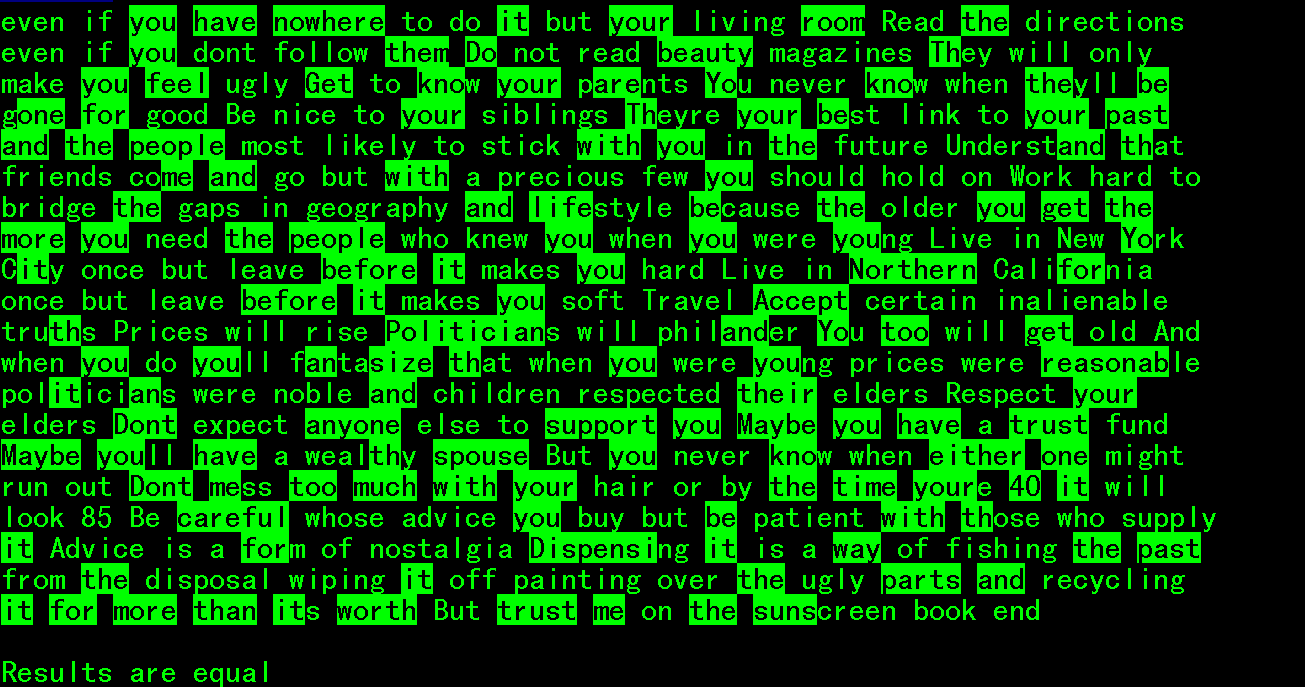
\includegraphics[angle=270,origin=b,width=0.70\textwidth]{string.eps}
\caption{String search}
\end{figure}

\begin{screen}
\tiny
\begin{verbatim}
orig()
{
  int i;
  printf("<<<ORIG>>>\n");
  for (i=0; i<snum; i++) {
    init_search(i);
    strsearch(i);
  }
  return 0;
}
init_search(int i)/* for ARM */
{
  char *str = sstr[i];
  int  len  = slen[i];
  int  j;
  for (j = 0; j <= UCHAR_MAX; j++)
    table[j] = len;
  for (j = 0; j < len; j++)
    table[(Uchar)str[j]] = len - j - 1;
  for (j = 0; j < clen; j++)
    *(out0+clen*i+j) = 0;
}
strsearch(int i)
{
  char *str = sstr[i];
  int  len  = slen[i];
  register size_t shift;
  register size_t pos = len - 1;
  char   *found;
  while (pos < clen) {
    while (pos < clen && (shift = table[(unsigned char)target[pos]]) > 0)
      pos += shift;
    if (!shift) {
      if (!strncmp(str, &target[pos-len+1], len))
        out0[i*clen+(pos-len+1)] = 0xff;
      pos++;
} } }
\end{verbatim}
\end{screen}

\begin{screen}
\tiny
\begin{verbatim}
imax()
{
  int i, j;
  printf("<<<IMAX>>>\n");
  for (i=0; i<snum; i++) {
    for (j=0; j<clen; j++) {
      if (!strncmp(sstr[i], &target[j], slen[i]))
        out1[i*clen+j] = 0xff;
      else
        out1[i*clen+j] = 0;
} } }
\end{verbatim}
\end{screen}

\begin{screen}
\tiny
\begin{verbatim}
imax()
{
  Ull   CHIP;
  Ull   LOOP1, LOOP0;
  Ull   INIT1, INIT0;
  Ull   AR[64][4];                     /* output of EX     in each unit */
  Ull   BR[64][4][4];                  /* output registers in each unit */
  Ull   r00, r01, r02, r03, r04, r05, r06, r07, r08, r09, r10, r11, r12, r13, r14, r15;
  Ull   r16, r17, r18, r19, r20, r21, r22, r23, r24, r25, r26, r27, r28, r29, r30, r31;
  Ull   c0, c1, c2, c3, ex0, ex1;
  Ull   t0[NCHIP], t1[NCHIP], t2[NCHIP], t3[NCHIP], t4[NCHIP], t5[NCHIP], t6[NCHIP], t7[NCHIP], t8[NCHIP];
  Ull   t0t[NCHIP], t1t[NCHIP], t2t[NCHIP], t3t[NCHIP], t4t[NCHIP], t5t[NCHIP], t6t[NCHIP], t7t[NCHIP], t8t[NCHIP];
  Ull   r0[NCHIP], r1[NCHIP], r2[NCHIP], r3[NCHIP], r4[NCHIP], r5[NCHIP], r6[NCHIP], r7[NCHIP], r8[NCHIP];
  Ull   r0t[NCHIP], r1t[NCHIP], r2t[NCHIP], r3t[NCHIP], r4t[NCHIP], r5t[NCHIP], r6t[NCHIP], r7t[NCHIP], r8t[NCHIP];
  Ull   i, dmy, loop=clen/NCHIP;
  Ull   dwi = clen/NCHIP/4+1; /* dwords */
  Ull   dwo = clen/NCHIP/4  ; /* dwords */

  printf("<<<IMAX>>>\n");
  for (CHIP=0; CHIP<NCHIP; CHIP++) {
    t0t[CHIP]=target+(clen/NCHIP*CHIP);
    t1t[CHIP]=target+(clen/NCHIP*CHIP);
    t2t[CHIP]=target+(clen/NCHIP*CHIP);
    t3t[CHIP]=target+(clen/NCHIP*CHIP);
    t4t[CHIP]=target+(clen/NCHIP*CHIP);
    t5t[CHIP]=target+(clen/NCHIP*CHIP);
    t6t[CHIP]=target+(clen/NCHIP*CHIP);
    t7t[CHIP]=target+(clen/NCHIP*CHIP);
    t8t[CHIP]=target+(clen/NCHIP*CHIP);
  }
  for (i=0; i<snum; i+=OMAP) {
    Ull  c00=sstr[i+0][0], c01=sstr[i+0][1], c02=sstr[i+0][2], c03=sstr[i+0][3], c04=sstr[i+0][4], c05=sstr[i+0][5], c06=sstr[i+0][6], c07=sstr[i+0][7];
    Ull  c10=sstr[i+1][0], c11=sstr[i+1][1], c12=sstr[i+1][2], c13=sstr[i+1][3], c14=sstr[i+1][4], c15=sstr[i+1][5], c16=sstr[i+1][6], c17=sstr[i+1][7];
         :
    Ull  c80=sstr[i+8][0], c81=sstr[i+8][1], c82=sstr[i+8][2], c83=sstr[i+8][3], c84=sstr[i+8][4], c85=sstr[i+8][5], c86=sstr[i+8][6], c87=sstr[i+8][7];
    Ull  slen0=slen[i+0], slen1=slen[i+1], slen2=slen[i+2], slen3=slen[i+3], slen4=slen[i+4], slen5=slen[i+5], slen6=slen[i+6], slen7=slen[i+7], slen8=slen[i+8];
    for (CHIP=0; CHIP<NCHIP; CHIP++) {
      t0[CHIP] = t0t[CHIP]-1;
      t1[CHIP] = t1t[CHIP]-1;
        :
      t8[CHIP] = t8t[CHIP]-1;
      r0[CHIP] = r0t[CHIP] = out1+(i+0)*clen+(clen/NCHIP*CHIP);
      r1[CHIP] = r1t[CHIP] = out1+(i+1)*clen+(clen/NCHIP*CHIP);
        :
      r8[CHIP] = r8t[CHIP] = out1+(i+8)*clen+(clen/NCHIP*CHIP);
    }
//EMAX5A begin search mapdist=0
    for (CHIP=0; CHIP<NCHIP; CHIP++) { //���å������ϸ����о�ʸ����礭������
      for (INIT0=1,LOOP0=loop,dmy=0; LOOP0--; INIT0=0) { //Ĺ����64KBʸ���ޤ�
      /* map#0 */
/*@0,1*/ exe(OP_ADD,       &t0[CHIP],     t0[CHIP], EXP_H3210,   1LL,          EXP_H3210, 0LL, EXP_H3210, OP_AND, 0x00000000ffffffffLL, OP_NOP, 0LL);
/*@1,0*/ exe(OP_MCAS,      &r00,          slen0,    EXP_H3210,   1,            EXP_H3210, 0LL, EXP_H3210, OP_NOP, 0LL,    OP_NOP,  0LL);
/*@1,1*/ exe(OP_MCAS,      &r01,          slen0,    EXP_H3210,   2,            EXP_H3210, 0LL, EXP_H3210, OP_NOP, 0LL,    OP_NOP,  0LL);
/*@1,2*/ exe(OP_MCAS,      &r02,          slen0,    EXP_H3210,   3,            EXP_H3210, 0LL, EXP_H3210, OP_NOP, 0LL,    OP_NOP,  0LL);
/*@1,3*/ exe(OP_MCAS,      &r03,          slen0,    EXP_H3210,   4,            EXP_H3210, 0LL, EXP_H3210, OP_NOP, 0LL,    OP_NOP,  0LL);
/*@1,0*/ mop(OP_LDBR,  1,  &BR[1][0][1],  t0[CHIP], 0,   MSK_D0, t0t[CHIP],    dwi,  0,   0,   (Ull)NULL,  dwi);
/*@1,0*/ mop(OP_LDBR,  1,  &BR[1][0][0],  t0[CHIP], 1,   MSK_D0, t0t[CHIP],    dwi,  0,   0,   (Ull)NULL,  dwi);
/*@1,1*/ mop(OP_LDBR,  1,  &BR[1][1][1],  t0[CHIP], 2,   MSK_D0, t0t[CHIP],    dwi,  0,   0,   (Ull)NULL,  dwi);
/*@1,1*/ mop(OP_LDBR,  1,  &BR[1][1][0],  t0[CHIP], 3,   MSK_D0, t0t[CHIP],    dwi,  0,   0,   (Ull)NULL,  dwi);
/*@1,2*/ mop(OP_LDBR,  1,  &BR[1][2][1],  t0[CHIP], 4,   MSK_D0, t0t[CHIP],    dwi,  0,   0,   (Ull)NULL,  dwi);
/*@1,2*/ mop(OP_LDBR,  1,  &BR[1][2][0],  t0[CHIP], 5,   MSK_D0, t0t[CHIP],    dwi,  0,   0,   (Ull)NULL,  dwi);
/*@1,3*/ mop(OP_LDBR,  1,  &BR[1][3][1],  t0[CHIP], 6,   MSK_D0, t0t[CHIP],    dwi,  0,   0,   (Ull)NULL,  dwi);
/*@1,3*/ mop(OP_LDBR,  1,  &BR[1][3][0],  t0[CHIP], 7,   MSK_D0, t0t[CHIP],    dwi,  0,   0,   (Ull)NULL,  dwi);
/*@2,0*/ exe(OP_CMP_NE,    &r16,          c00,      EXP_H3210,   BR[1][0][1],  EXP_H3210, 0LL, EXP_H3210, OP_AND, r00,    OP_NOP,  0LL); // 1 if unmatch
/*@2,1*/ exe(OP_CMP_NE,    &r17,          c01,      EXP_H3210,   BR[1][0][0],  EXP_H3210, 0LL, EXP_H3210, OP_AND, r01,    OP_NOP,  0LL); // 1 if unmatch
/*@2,2*/ exe(OP_CMP_NE,    &r18,          c02,      EXP_H3210,   BR[1][1][1],  EXP_H3210, 0LL, EXP_H3210, OP_AND, r02,    OP_NOP,  0LL); // 1 if unmatch
/*@2,3*/ exe(OP_CMP_NE,    &r19,          c03,      EXP_H3210,   BR[1][1][0],  EXP_H3210, 0LL, EXP_H3210, OP_AND, r03,    OP_NOP,  0LL); // 1 if unmatch
/*@3,0*/ exe(OP_MCAS,      &r04,          slen0,    EXP_H3210,   5,            EXP_H3210, 0LL, EXP_H3210, OP_NOP, 0LL,    OP_NOP,  0LL);
/*@3,1*/ exe(OP_MCAS,      &r05,          slen0,    EXP_H3210,   6,            EXP_H3210, 0LL, EXP_H3210, OP_NOP, 0LL,    OP_NOP,  0LL);
/*@3,2*/ exe(OP_MCAS,      &r06,          slen0,    EXP_H3210,   7,            EXP_H3210, 0LL, EXP_H3210, OP_NOP, 0LL,    OP_NOP,  0LL);
/*@3,3*/ exe(OP_MCAS,      &r07,          slen0,    EXP_H3210,   8,            EXP_H3210, 0LL, EXP_H3210, OP_NOP, 0LL,    OP_NOP,  0LL);
/*@4,0*/ exe(OP_CMP_NE,    &r20,          c04,      EXP_H3210,   BR[1][2][1],  EXP_H3210, 0LL, EXP_H3210, OP_AND, r04,    OP_NOP,  0LL); // 1 if unmatch
/*@4,1*/ exe(OP_CMP_NE,    &r21,          c05,      EXP_H3210,   BR[1][2][0],  EXP_H3210, 0LL, EXP_H3210, OP_AND, r05,    OP_NOP,  0LL); // 1 if unmatch
/*@4,2*/ exe(OP_CMP_NE,    &r22,          c06,      EXP_H3210,   BR[1][3][1],  EXP_H3210, 0LL, EXP_H3210, OP_AND, r06,    OP_NOP,  0LL); // 1 if unmatch
/*@4,3*/ exe(OP_CMP_NE,    &r23,          c07,      EXP_H3210,   BR[1][3][0],  EXP_H3210, 0LL, EXP_H3210, OP_AND, r07,    OP_NOP,  0LL); // 1 if unmatch
/*@5,0*/ exe(OP_ADD3,      &r10,          r16,      EXP_H3210,   r17,          EXP_H3210, r18, EXP_H3210, OP_NOP, 0LL,    OP_NOP,  0LL); //
/*@5,1*/ exe(OP_ADD3,      &r11,          r19,      EXP_H3210,   r20,          EXP_H3210, r21, EXP_H3210, OP_NOP, 0LL,    OP_NOP,  0LL); //
/*@5,2*/ exe(OP_ADD,       &r12,          r22,      EXP_H3210,   r23,          EXP_H3210, 0LL, EXP_H3210, OP_NOP, 0LL,    OP_NOP,  0LL); //
/*@6,0*/ exe(OP_ADD3,      &r00,          r10,      EXP_H3210,   r11,          EXP_H3210, r12, EXP_H3210, OP_NOP, 0LL,    OP_NOP,  0LL); //
/*@7,0*/ exe(OP_MCAS,      &r31,          0LL,      EXP_H3210,   r00,          EXP_H3210, 0LL, EXP_H3210, OP_NOP, 0LL,    OP_NOP,  0LL); // FF if match
/*@7,0*/ mop(OP_STBR, 3,   &r31,          r0[CHIP]++, 0, MSK_D0, r0t[CHIP],    dwo,  0,   0,   (Ull)NULL,  dwo);
        :
      /* map#8 */
/*@56,1*/exe(OP_ADD,       &t8[CHIP],     t8[CHIP], EXP_H3210,   1LL,          EXP_H3210, 0LL, EXP_H3210, OP_AND, 0x00000000ffffffffLL, OP_NOP, 0LL);
/*@57,0*/exe(OP_MCAS,      &r00,          slen8,    EXP_H3210,   1,            EXP_H3210, 0LL, EXP_H3210, OP_NOP, 0LL,    OP_NOP,  0LL);
/*@57,1*/exe(OP_MCAS,      &r01,          slen8,    EXP_H3210,   2,            EXP_H3210, 0LL, EXP_H3210, OP_NOP, 0LL,    OP_NOP,  0LL);
/*@57,2*/exe(OP_MCAS,      &r02,          slen8,    EXP_H3210,   3,            EXP_H3210, 0LL, EXP_H3210, OP_NOP, 0LL,    OP_NOP,  0LL);
/*@57,3*/exe(OP_MCAS,      &r03,          slen8,    EXP_H3210,   4,            EXP_H3210, 0LL, EXP_H3210, OP_NOP, 0LL,    OP_NOP,  0LL);
/*@57,0*/mop(OP_LDBR,  1,  &BR[57][0][1], t8[CHIP], 0,   MSK_D0, t7t[CHIP],    dwi,  0,   0,   (Ull)NULL,  dwi);
/*@57,0*/mop(OP_LDBR,  1,  &BR[57][0][0], t8[CHIP], 1,   MSK_D0, t7t[CHIP],    dwi,  0,   0,   (Ull)NULL,  dwi);
/*@57,1*/mop(OP_LDBR,  1,  &BR[57][1][1], t8[CHIP], 2,   MSK_D0, t7t[CHIP],    dwi,  0,   0,   (Ull)NULL,  dwi);
/*@57,1*/mop(OP_LDBR,  1,  &BR[57][1][0], t8[CHIP], 3,   MSK_D0, t7t[CHIP],    dwi,  0,   0,   (Ull)NULL,  dwi);
/*@57,2*/mop(OP_LDBR,  1,  &BR[57][2][1], t8[CHIP], 4,   MSK_D0, t7t[CHIP],    dwi,  0,   0,   (Ull)NULL,  dwi);
/*@57,2*/mop(OP_LDBR,  1,  &BR[57][2][0], t8[CHIP], 5,   MSK_D0, t7t[CHIP],    dwi,  0,   0,   (Ull)NULL,  dwi);
/*@57,3*/mop(OP_LDBR,  1,  &BR[57][3][1], t8[CHIP], 6,   MSK_D0, t7t[CHIP],    dwi,  0,   0,   (Ull)NULL,  dwi);
/*@57,3*/mop(OP_LDBR,  1,  &BR[57][3][0], t8[CHIP], 7,   MSK_D0, t7t[CHIP],    dwi,  0,   0,   (Ull)NULL,  dwi);
/*@58,0*/exe(OP_CMP_NE,    &r16,          c80,      EXP_H3210,   BR[57][0][1], EXP_H3210, 0LL, EXP_H3210, OP_AND, r00,    OP_NOP,  0LL); // 1 if unmatch
/*@58,1*/exe(OP_CMP_NE,    &r17,          c81,      EXP_H3210,   BR[57][0][0], EXP_H3210, 0LL, EXP_H3210, OP_AND, r01,    OP_NOP,  0LL); // 1 if unmatch
/*@58,2*/exe(OP_CMP_NE,    &r18,          c82,      EXP_H3210,   BR[57][1][1], EXP_H3210, 0LL, EXP_H3210, OP_AND, r02,    OP_NOP,  0LL); // 1 if unmatch
/*@58,3*/exe(OP_CMP_NE,    &r19,          c83,      EXP_H3210,   BR[57][1][0], EXP_H3210, 0LL, EXP_H3210, OP_AND, r03,    OP_NOP,  0LL); // 1 if unmatch
/*@59,0*/exe(OP_MCAS,      &r04,          slen8,    EXP_H3210,   5,            EXP_H3210, 0LL, EXP_H3210, OP_NOP, 0LL,    OP_NOP,  0LL);
/*@59,1*/exe(OP_MCAS,      &r05,          slen8,    EXP_H3210,   6,            EXP_H3210, 0LL, EXP_H3210, OP_NOP, 0LL,    OP_NOP,  0LL);
/*@59,2*/exe(OP_MCAS,      &r06,          slen8,    EXP_H3210,   7,            EXP_H3210, 0LL, EXP_H3210, OP_NOP, 0LL,    OP_NOP,  0LL);
/*@59,3*/exe(OP_MCAS,      &r07,          slen8,    EXP_H3210,   8,            EXP_H3210, 0LL, EXP_H3210, OP_NOP, 0LL,    OP_NOP,  0LL);
/*@60,0*/exe(OP_CMP_NE,    &r20,          c84,      EXP_H3210,   BR[57][2][1], EXP_H3210, 0LL, EXP_H3210, OP_AND, r04,    OP_NOP,  0LL); // 1 if unmatch
/*@60,1*/exe(OP_CMP_NE,    &r21,          c85,      EXP_H3210,   BR[57][2][0], EXP_H3210, 0LL, EXP_H3210, OP_AND, r05,    OP_NOP,  0LL); // 1 if unmatch
/*@60,2*/exe(OP_CMP_NE,    &r22,          c86,      EXP_H3210,   BR[57][3][1], EXP_H3210, 0LL, EXP_H3210, OP_AND, r06,    OP_NOP,  0LL); // 1 if unmatch
/*@60,3*/exe(OP_CMP_NE,    &r23,          c87,      EXP_H3210,   BR[57][3][0], EXP_H3210, 0LL, EXP_H3210, OP_AND, r07,    OP_NOP,  0LL); // 1 if unmatch
/*@61,0*/exe(OP_ADD3,      &r10,          r16,      EXP_H3210,   r17,          EXP_H3210, r18, EXP_H3210, OP_NOP, 0LL,    OP_NOP,  0LL); //
/*@61,1*/exe(OP_ADD3,      &r11,          r19,      EXP_H3210,   r20,          EXP_H3210, r21, EXP_H3210, OP_NOP, 0LL,    OP_NOP,  0LL); //
/*@61,2*/exe(OP_ADD,       &r12,          r22,      EXP_H3210,   r23,          EXP_H3210, 0LL, EXP_H3210, OP_NOP, 0LL,    OP_NOP,  0LL); //
/*@62,0*/exe(OP_ADD3,      &r00,          r10,      EXP_H3210,   r11,          EXP_H3210, r12, EXP_H3210, OP_NOP, 0LL,    OP_NOP,  0LL); //
/*@63,0*/exe(OP_MCAS,      &r31,          0LL,      EXP_H3210,   r00,          EXP_H3210, 0LL, EXP_H3210, OP_NOP, 0LL,    OP_NOP,  0LL); // FF if match
/*@63,0*/mop(OP_STBR, 3,   &r31,          r8[CHIP]++, 0, MSK_D0, r8t[CHIP],    dwo,  0,   0,   (Ull)NULL,  dwo);
      }
    }
//EMAX5A end
//EMAX5A drain_dirty_lmm
  }
}
\end{verbatim}
\end{screen}

\begin{figure}[htbp]
\center
\epsfile{file=pbmsrch+rmm-search-emax6.eps,width=1.00\textwidth}
\caption{ʸ���󸡺�}
\end{figure}

\clearpage

\subsection{16x16���߹���}

\shabox{
\leftline{cent\% make -f Makefile-csim.emax6+dma all clean}
\leftline{cent\% ../../src/csim/csim -x conv16-csim.emax6+dma}
}

\shabox{
\leftline{zynq\% make -f Makefile-zynq.emax6+dma all clean}
\leftline{zynq\% ./conv16-zynq.emax6+dma}
}

\vskip .1in

16x16�ξ��߹��߱黻�Ǥ��롥���٤ΥС����ȱ黻�ˤ��1��ʬ�Τ߷׻����롥���ƥ�
����׻��Ǥ���mapdist=2�Ǥ��롥

\begin{screen}
\tiny
\begin{verbatim}
conv16_x1(float *yi, float *yo)
{
 Ull  loop = image_WD/2-8;
 Ull  x = 8;
#if !defined(EMAX5) && !defined(EMAX6)
 while (loop--) {
 yo[x]= yim8[x-8]*SCON[  0]+yim8[x-7]*SCON[  1]+yim8[x-6]*SCON[  2]+yim8[x-5]*SCON[  3]+yim8[x-4]*SCON[  4]+yim8[x-3]*SCON[  5]+yim8[x-2]*SCON[  6]+yim8[x-1]*SCON[  7]
      + yim8[x+0]*SCON[  8]+yim8[x+1]*SCON[  9]+yim8[x+2]*SCON[ 10]+yim8[x+3]*SCON[ 11]+yim8[x+4]*SCON[ 12]+yim8[x+5]*SCON[ 13]+yim8[x+6]*SCON[ 14]+yim8[x+7]*SCON[ 15]
      + yim7[x-8]*SCON[ 16]+yim7[x-7]*SCON[ 17]+yim7[x-6]*SCON[ 18]+yim7[x-5]*SCON[ 19]+yim7[x-4]*SCON[ 20]+yim7[x-3]*SCON[ 21]+yim7[x-2]*SCON[ 22]+yim7[x-1]*SCON[ 23]
      + yim7[x+0]*SCON[ 24]+yim7[x+1]*SCON[ 25]+yim7[x+2]*SCON[ 26]+yim7[x+3]*SCON[ 27]+yim7[x+4]*SCON[ 28]+yim7[x+5]*SCON[ 29]+yim7[x+6]*SCON[ 30]+yim7[x+7]*SCON[ 31]
      + yim6[x-8]*SCON[ 32]+yim6[x-7]*SCON[ 33]+yim6[x-6]*SCON[ 34]+yim6[x-5]*SCON[ 35]+yim6[x-4]*SCON[ 36]+yim6[x-3]*SCON[ 37]+yim6[x-2]*SCON[ 38]+yim6[x-1]*SCON[ 39]
      :
      + yip1[x+0]*SCON[152]+yip1[x+1]*SCON[153]+yip1[x+2]*SCON[154]+yip1[x+3]*SCON[155]+yip1[x+4]*SCON[156]+yip1[x+5]*SCON[157]+yip1[x+6]*SCON[158]+yip1[x+7]*SCON[159]
      + yip2[x-8]*SCON[160]+yip2[x-7]*SCON[161]+yip2[x-6]*SCON[162]+yip2[x-5]*SCON[163]+yip2[x-4]*SCON[164]+yip2[x-3]*SCON[165]+yip2[x-2]*SCON[166]+yip2[x-1]*SCON[167]
      + yip2[x+0]*SCON[168]+yip2[x+1]*SCON[169]+yip2[x+2]*SCON[170]+yip2[x+3]*SCON[171]+yip2[x+4]*SCON[172]+yip2[x+5]*SCON[173]+yip2[x+6]*SCON[174]+yip2[x+7]*SCON[175]
      + yip3[x-8]*SCON[176]+yip3[x-7]*SCON[177]+yip3[x-6]*SCON[178]+yip3[x-5]*SCON[179]+yip3[x-4]*SCON[180]+yip3[x-3]*SCON[181]+yip3[x-2]*SCON[182]+yip3[x-1]*SCON[183]
      + yip3[x+0]*SCON[184]+yip3[x+1]*SCON[185]+yip3[x+2]*SCON[186]+yip3[x+3]*SCON[187]+yip3[x+4]*SCON[188]+yip3[x+5]*SCON[189]+yip3[x+6]*SCON[190]+yip3[x+7]*SCON[191]
      + yip4[x-8]*SCON[192]+yip4[x-7]*SCON[193]+yip4[x-6]*SCON[194]+yip4[x-5]*SCON[195]+yip4[x-4]*SCON[196]+yip4[x-3]*SCON[197]+yip4[x-2]*SCON[198]+yip4[x-1]*SCON[199]
      + yip4[x+0]*SCON[200]+yip4[x+1]*SCON[201]+yip4[x+2]*SCON[202]+yip4[x+3]*SCON[203]+yip4[x+4]*SCON[204]+yip4[x+5]*SCON[205]+yip4[x+6]*SCON[206]+yip4[x+7]*SCON[207]
      + yip5[x-8]*SCON[208]+yip5[x-7]*SCON[209]+yip5[x-6]*SCON[210]+yip5[x-5]*SCON[211]+yip5[x-4]*SCON[212]+yip5[x-3]*SCON[213]+yip5[x-2]*SCON[214]+yip5[x-1]*SCON[215]
      + yip5[x+0]*SCON[216]+yip5[x+1]*SCON[217]+yip5[x+2]*SCON[218]+yip5[x+3]*SCON[219]+yip5[x+4]*SCON[220]+yip5[x+5]*SCON[221]+yip5[x+6]*SCON[222]+yip5[x+7]*SCON[223]
      + yip6[x-8]*SCON[224]+yip6[x-7]*SCON[225]+yip6[x-6]*SCON[226]+yip6[x-5]*SCON[227]+yip6[x-4]*SCON[228]+yip6[x-3]*SCON[229]+yip6[x-2]*SCON[230]+yip6[x-1]*SCON[231]
      + yip6[x+0]*SCON[232]+yip6[x+1]*SCON[233]+yip6[x+2]*SCON[234]+yip6[x+3]*SCON[235]+yip6[x+4]*SCON[236]+yip6[x+5]*SCON[237]+yip6[x+6]*SCON[238]+yip6[x+7]*SCON[239]
      + yip7[x-8]*SCON[240]+yip7[x-7]*SCON[241]+yip7[x-6]*SCON[242]+yip7[x-5]*SCON[243]+yip7[x-4]*SCON[244]+yip7[x-3]*SCON[245]+yip7[x-2]*SCON[246]+yip7[x-1]*SCON[247]
      + yip7[x+0]*SCON[248]+yip7[x+1]*SCON[249]+yip7[x+2]*SCON[250]+yip7[x+3]*SCON[251]+yip7[x+4]*SCON[252]+yip7[x+5]*SCON[253]+yip7[x+6]*SCON[254]+yip7[x+7]*SCON[255];
 x += 2;
 }
#endif
\end{verbatim}
\end{screen}

\begin{screen}
\tiny
\begin{verbatim}
  Ull  AR[64][4];                     /* output of EX     in each unit */
  Ull  BR[64][4][4];                  /* output registers in each unit */
  Ull  r0, r1, r2, r3, r4, r5, r6, r7, r8, r9, r10, r11, r12, r13, r14, r15;
  Ull  r16, r17, r18, r19, r20, r21, r22, r23, r24, r25, r26, r27, r28, r29, r30, r31;
  Ull c000=DCON[  0], c002=DCON[  1], c004=DCON[  2], c006=DCON[  3], c008=DCON[  4], c010=DCON[  5], c012=DCON[  6], c014=DCON[  7];
  Ull c016=DCON[  8], c018=DCON[  9], c020=DCON[ 10], c022=DCON[ 11], c024=DCON[ 12], c026=DCON[ 13], c028=DCON[ 14], c030=DCON[ 15];
  Ull c032=DCON[ 16], c034=DCON[ 17], c036=DCON[ 18], c038=DCON[ 19], c040=DCON[ 20], c042=DCON[ 21], c044=DCON[ 22], c046=DCON[ 23];
  Ull c048=DCON[ 24], c050=DCON[ 25], c052=DCON[ 26], c054=DCON[ 27], c056=DCON[ 28], c058=DCON[ 29], c060=DCON[ 30], c062=DCON[ 31];
  Ull c064=DCON[ 32], c066=DCON[ 33], c068=DCON[ 34], c070=DCON[ 35], c072=DCON[ 36], c074=DCON[ 37], c076=DCON[ 38], c078=DCON[ 39];
       :
  Ull c240=DCON[120], c242=DCON[121], c244=DCON[122], c246=DCON[123], c248=DCON[124], c250=DCON[125], c252=DCON[126], c254=DCON[127];
//EMAX5A begin x1 mapdist=2
  while (loop--) {                                  /* mapped to WHILE() on BR[15][0][0] stage#0 */
    mop(OP_LDR,  3, &BR[0][0][1], yim80++, 0, MSK_D0, yim80, 320, 0, 0, (Ull)NULL, 320); /* stage#0 */
    mop(OP_LDR,  3, &r1,          yim81++, 0, MSK_D0, yim80, 320, 0, 0, (Ull)NULL, 320); /* stage#0 */
    mop(OP_LDR,  3, &r2,          yim82++, 0, MSK_D0, yim80, 320, 0, 0, (Ull)NULL, 320); /* stage#0 */
    mop(OP_LDR,  3, &r3,          yim83++, 0, MSK_D0, yim80, 320, 0, 0, (Ull)NULL, 320); /* stage#0 */
    mop(OP_LDR,  3, &r4,          yim84++, 0, MSK_D0, yim80, 320, 0, 0, (Ull)NULL, 320); /* stage#0 */
    mop(OP_LDR,  3, &r5,          yim85++, 0, MSK_D0, yim80, 320, 0, 0, (Ull)NULL, 320); /* stage#0 */
    mop(OP_LDR,  3, &r6,          yim86++, 0, MSK_D0, yim80, 320, 0, 0, (Ull)NULL, 320); /* stage#0 */
    mop(OP_LDR,  3, &r7,          yim87++, 0, MSK_D0, yim80, 320, 0, 0, (Ull)NULL, 320); /* stage#0 */
    exe(OP_FMA, &r10, 0LL, EXP_H3210, BR[0][0][1], EXP_H3210, c000, EXP_H3210, OP_NOP, 0LL, OP_NOP, 0LL); /* stage#1 */
    exe(OP_FMA, &r11, 0LL, EXP_H3210, r1,          EXP_H3210, c002, EXP_H3210, OP_NOP, 0LL, OP_NOP, 0LL); /* stage#1 */
    exe(OP_FMA, &r12, 0LL, EXP_H3210, r2,          EXP_H3210, c004, EXP_H3210, OP_NOP, 0LL, OP_NOP, 0LL); /* stage#1 */
    exe(OP_FMA, &r13, 0LL, EXP_H3210, r3,          EXP_H3210, c006, EXP_H3210, OP_NOP, 0LL, OP_NOP, 0LL); /* stage#1 */
    exe(OP_FMA, &r20, r10, EXP_H3210, r4,          EXP_H3210, c008, EXP_H3210, OP_NOP, 0LL, OP_NOP, 0LL); /* stage#2 */
    exe(OP_FMA, &r21, r11, EXP_H3210, r5,          EXP_H3210, c010, EXP_H3210, OP_NOP, 0LL, OP_NOP, 0LL); /* stage#2 */
    exe(OP_FMA, &r22, r12, EXP_H3210, r6,          EXP_H3210, c012, EXP_H3210, OP_NOP, 0LL, OP_NOP, 0LL); /* stage#2 */
    exe(OP_FMA, &r23, r13, EXP_H3210, r7,          EXP_H3210, c014, EXP_H3210, OP_NOP, 0LL, OP_NOP, 0LL); /* stage#2 */
    mop(OP_LDR,  3, &BR[2][0][1], yim70++, 0, MSK_D0, yim70, 320, 0, 0, (Ull)NULL, 320); /* stage#2 */
    mop(OP_LDR,  3, &r1,          yim71++, 0, MSK_D0, yim70, 320, 0, 0, (Ull)NULL, 320); /* stage#2 */
    mop(OP_LDR,  3, &r2,          yim72++, 0, MSK_D0, yim70, 320, 0, 0, (Ull)NULL, 320); /* stage#2 */
    mop(OP_LDR,  3, &r3,          yim73++, 0, MSK_D0, yim70, 320, 0, 0, (Ull)NULL, 320); /* stage#2 */
    mop(OP_LDR,  3, &r4,          yim74++, 0, MSK_D0, yim70, 320, 0, 0, (Ull)NULL, 320); /* stage#2 */
    mop(OP_LDR,  3, &r5,          yim75++, 0, MSK_D0, yim70, 320, 0, 0, (Ull)NULL, 320); /* stage#2 */
    mop(OP_LDR,  3, &r6,          yim76++, 0, MSK_D0, yim70, 320, 0, 0, (Ull)NULL, 320); /* stage#2 */
    mop(OP_LDR,  3, &r7,          yim77++, 0, MSK_D0, yim70, 320, 0, 0, (Ull)NULL, 320); /* stage#2 */
        :
    exe(OP_FMA, &r10, r20, EXP_H3210, BR[30][0][1],EXP_H3210, c240, EXP_H3210, OP_NOP, 0LL, OP_NOP, 0LL); /* stage#31 */
    exe(OP_FMA, &r11, r21, EXP_H3210, r1,          EXP_H3210, c242, EXP_H3210, OP_NOP, 0LL, OP_NOP, 0LL); /* stage#31 */
    exe(OP_FMA, &r12, r22, EXP_H3210, r2,          EXP_H3210, c244, EXP_H3210, OP_NOP, 0LL, OP_NOP, 0LL); /* stage#31 */
    exe(OP_FMA, &r13, r23, EXP_H3210, r3,          EXP_H3210, c246, EXP_H3210, OP_NOP, 0LL, OP_NOP, 0LL); /* stage#31 */
    exe(OP_FMA, &r20, r10, EXP_H3210, r4,          EXP_H3210, c248, EXP_H3210, OP_NOP, 0LL, OP_NOP, 0LL); /* stage#32 */
    exe(OP_FMA, &r21, r11, EXP_H3210, r5,          EXP_H3210, c250, EXP_H3210, OP_NOP, 0LL, OP_NOP, 0LL); /* stage#32 */
    exe(OP_FMA, &r22, r12, EXP_H3210, r6,          EXP_H3210, c252, EXP_H3210, OP_NOP, 0LL, OP_NOP, 0LL); /* stage#32 */
    exe(OP_FMA, &r23, r13, EXP_H3210, r7,          EXP_H3210, c254, EXP_H3210, OP_NOP, 0LL, OP_NOP, 0LL); /* stage#32 */

    exe(OP_FAD, &r10,  r20, EXP_H3210,  r21, EXP_H3210, 0LL, EXP_H3210, OP_NOP, 0LL, OP_NOP, 0LL);        /* stage#33 */
    exe(OP_FAD, &r12,  r22, EXP_H3210,  r23, EXP_H3210, 0LL, EXP_H3210, OP_NOP, 0LL, OP_NOP, 0LL);        /* stage#33 */
    exe(OP_FAD, &AR[35][0],  r10, EXP_H3210,  r12, EXP_H3210, 0LL, EXP_H3210, OP_NOP, 0LL, OP_NOP, 0LL);  /* stage#35 */
    mop(OP_STR, 3, &AR[35][0], yoo++, 0LL, MSK_D0, (Ull)yoo, 152, 0, 0, yop, 152);                        /* stage#35 */
  }
//EMAX5A end
#endif
}
\end{verbatim}
\end{screen}

\begin{figure}[htbp]
\center
\epsfile{file=conv16-x1-emax6.eps,width=1.00\textwidth}
\caption{16x16���߹���}
\end{figure}

\clearpage

\subsection{VBGMM\_Logsum}

\shabox{
\leftline{cent\% make -f Makefile-csim.emax6+dma test016-csim.emax6+dma clean}
\leftline{cent\% ../../src/csim/csim -x test016-csim.emax6+dma}
}

\shabox{
\leftline{zynq\% make -f Makefile-zynq.emax6+dma test016-zynq.emax6+dma clean}
\leftline{zynq\% ./test016-zynq.emax6+dma}
}

\begin{screen}
\tiny
\begin{verbatim}
  for (chip=0; chip<NCHIP; chip++) { /* will be parallelized by multi-chip (M/#chip) */
    for (grp=M/NCHIP*chip; grp<M/NCHIP*(chip+1); grp+=RMGRP) { /* will be parallelized by multi-chip (M/#chip) */
      typedef struct {Uint i[4]} Ui4;
      Ui4  *c60 = C1+grp*M, *c600 = c60;
      Ull  row, bofs, rofs;
      Ull  b00;
      Ull  PARAM = 0x0000000100000001LL; /* 1 */
//EMAX5A begin x1 mapdist=0
/*2*/ for (INIT1=1,LOOP1=RMGRP,row=0-M*4; LOOP1--; INIT1=0) {                                                               /* stage#0 */
  /*1*/ for (INIT0=1,LOOP0=M/W,bofs=0-W*4; LOOP0--; INIT0=0) {                                                              /* stage#0 */
          exe(OP_ADD,    &bofs, INIT0?bofs:bofs, EXP_H3210, W*4, EXP_H3210, 0LL, EXP_H3210, OP_AND, 0x00000000ffffffffLL, OP_NOP, 0LL);/* stage#0 */
          exe(OP_ADD,    &row, row, EXP_H3210, INIT0?M*4:0, EXP_H3210, 0LL, EXP_H3210, OP_NOP, 0LL, OP_NOP, 0LL);           /* stage#0 */
          exe(OP_ADD,    &rofs, row, EXP_H3210, 0LL,  EXP_H3210, 0LL, EXP_H3210, OP_AND, 0x00000000ffffffffLL, OP_NOP, 0LL);/* stage#1 */

          mop(OP_LDWR,   1, &b00,  (Ull)c600, (Ull)rofs,  MSK_W0, (Ull)c60,  M*RMGRP, 0, 1, (Ull)NULL, M*RMGRP);            /* stage#2 */
          exe(OP_ADD,       &b00,  INIT0?b00:b00,   EXP_H3210,  PARAM,  EXP_H3210, 0LL,    EXP_H3210, OP_NOP, 0LL, OP_NOP, 0LL);  /* stage#2 */
          mop(OP_STWR,   1, &b00,  (Ull)rofs, (Ull)c600,  MSK_D0, (Ull)c60,  M*RMGRP, 0, 1, (Ull)NULL, M*RMGRP);            /* stage#2 */
        }
      }
//EMAX5A end
//EMAX5A drain_dirty_lmm
    }
  }
\end{verbatim}
\end{screen}

\clearpage

\subsection{Stochastic sgemm00}

\shabox{
\leftline{cent\% make -f Makefile-csim.emax6+dma test021-csim.emax6+dma clean}
\leftline{cent\% ../../src/csim/csim -x test021-csim.emax6+dma}
}

\shabox{
\leftline{zynq\% make -f Makefile-zynq.emax6+dma test021-zynq.emax6+dma clean}
\leftline{zynq\% ./test021-zynq.emax6+dma}
}

\begin{figure}[htbp]
\center
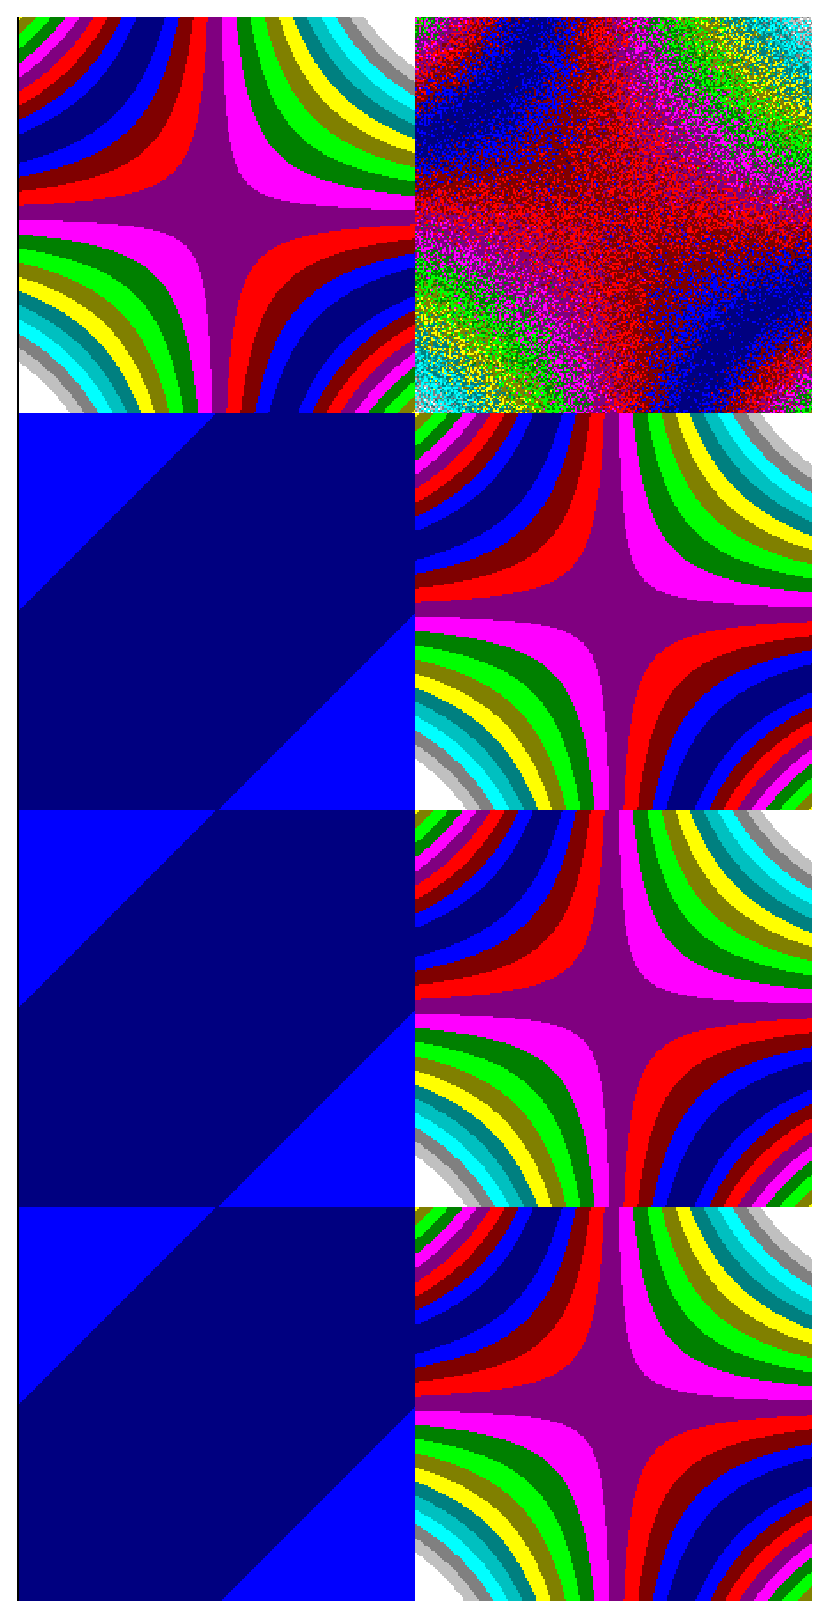
\includegraphics[angle=270,origin=b,width=0.75\textwidth]{stochastic.eps}
\caption{Stochastic sgemm00}
\end{figure}

\begin{screen}
\tiny
\begin{verbatim}
for (top=0; top<BS/NCHIP; top+=H) { /* will be parallelized by multi-chip (M/#chip) */
  for (blk=0; blk<OC4; blk+=RMGRP) { /* 3�ť롼��Ÿ���γ�¦�о� */
    char *a[H][NCHIP];
    char *b, *b0;
    char *c[H][NCHIP], *c0[H][NCHIP];
    b = (Uchar*)i_m0B+blk*IC32; b0 = b+IC32*0;
    for (CHIP=0; CHIP<NCHIP; CHIP++) { /* will be parallelized by multi-chip (M/#chip) */
      for (k=0; k<H; k++) {
        a[k][CHIP] = (Uchar*)i_m0A+(CHIP*BS/NCHIP+top+k)*IC32;
        c[k][CHIP] = (Uchar*)i_m0C+(CHIP*BS/NCHIP+top+k)*OC4+blk;
        c0[k][CHIP]= c[k][CHIP]+0;
      }
    }

#define spike01_core1(r, s) \
  mo4(OP_LDRQ,  1,  BR[r][2], (Ull)b0,                  (Ull)bofs,        MSK_W1,    (Ull)b,          IC32D4RMGRP, 0,      0,   (Ull)NULL, IC32D4RMGRP);/* stage#2 */\
  mo4(OP_LDRQ,  1,  BR[r][1], (Ull)a[s][CHIP],          (Ull)cofs,        MSK_W1,    (Ull)a[s][CHIP], IC32D4,      0,      0,   (Ull)NULL, IC32D4);     /* stage#2 */\
  exe(OP_NOP,      &AR[r][0], 0LL,           EXP_H3210, 0LL,              EXP_H3210, 0LL,             EXP_H3210,   OP_NOP, 0LL, OP_NOP,    0LL);        /* stage#2 */\
  mop(OP_LDBR,  1, &b00,      (Ull)c0[s][CHIP],         (Ull)oofs,        MSK_W0,    (Ull)c[s][CHIP], RMGRPD4,     0,      1,   (Ull)NULL, RMGRPD4);    /* stage#2 */\
  ex4(OP_SFMA,     &b00,      INIT0?b00:b00, EXP_H3210, BR[r][1],         EXP_H3210, BR[r][2],        EXP_H3210,   OP_NOP, 3LL, OP_NOP,    0LL);        /* stage#2 */\
  mop(OP_STBR,  1, &b00,      (Ull)oofs,                (Ull)c0[s][CHIP], MSK_D0,    (Ull)c[s][CHIP], RMGRPD4,     0,      1,   (Ull)NULL, RMGRPD4)     /* stage#2 */

//EMAX5A begin smax2 mapdist=0
  /*3*/ for (CHIP=0; CHIP<NCHIP; CHIP++) { /* will be parallelized by multi-chip (M/#chip) */
/*2*/ for (INIT1=1,LOOP1=RMGRP,rofs=(0-IC32)<<32|((0-1LL)&0xffffffff); LOOP1--; INIT1=0) {      /* stage#0 *//* mapped to FOR() on BR[63][1][0] */
  /*1*/ for (INIT0=1,LOOP0=IC32/32,cofs=(0-32LL)<<32|((0)&0xffffffff); LOOP0--; INIT0=0) {      /* stage#0 *//* mapped to FOR() on BR[63][0][0] */
          exe(OP_ADD,    &cofs, INIT0?cofs:cofs, EXP_H3210, (32LL)<<32|(0), EXP_H3210, 0LL, EXP_H3210, OP_AND, 0xffffffffffffffffLL, OP_NOP, 0LL); /* stage#0 */
          exe(OP_ADD,    &rofs, rofs, EXP_H3210, INIT0?IC321:0, EXP_H3210, 0LL, EXP_H3210, OP_NOP, 0LL, OP_NOP, 0LL);  /* stage#0 */
          exe(OP_ADD,    &bofs, rofs, EXP_H3210, cofs, EXP_H3210, 0, EXP_H3210, OP_AND, 0xffffffffffffffffLL, OP_NOP, 0LL);     /* stage#1 */
          exe(OP_ADD,    &oofs, rofs, EXP_H3210, cofs, EXP_H3210, 0, EXP_H3210, OP_AND, 0x00000000ffffffffLL, OP_NOP, 0LL);     /* stage#1 */

          spike01_core1( 2,  0);
          spike01_core1( 3,  1);
          spike01_core1( 4,  2);
          :
          spike01_core1(20, 18);
          spike01_core1(21, 19); /* H=20 */
          spike01_core1(22, 20);
          spike01_core1(23, 21);
          spike01_core1(24, 22);
          spike01_core1(25, 23);
          spike01_core1(26, 24); /* H=25 */
          :
          spike01_core1(50, 48);
          spike01_core1(51, 49); /* H=50 */
        }
      }
    }
//EMAX5A end
  }
}
//EMAX5A drain_dirty_lmm
\end{verbatim}
\end{screen}

\begin{figure}[htbp]
\center
\epsfile{file=smax-smax2-emax6.eps,width=1.00\textwidth}
\caption{Stochastic sgemm00}
\end{figure}

\begin{figure}[htbp]
\center
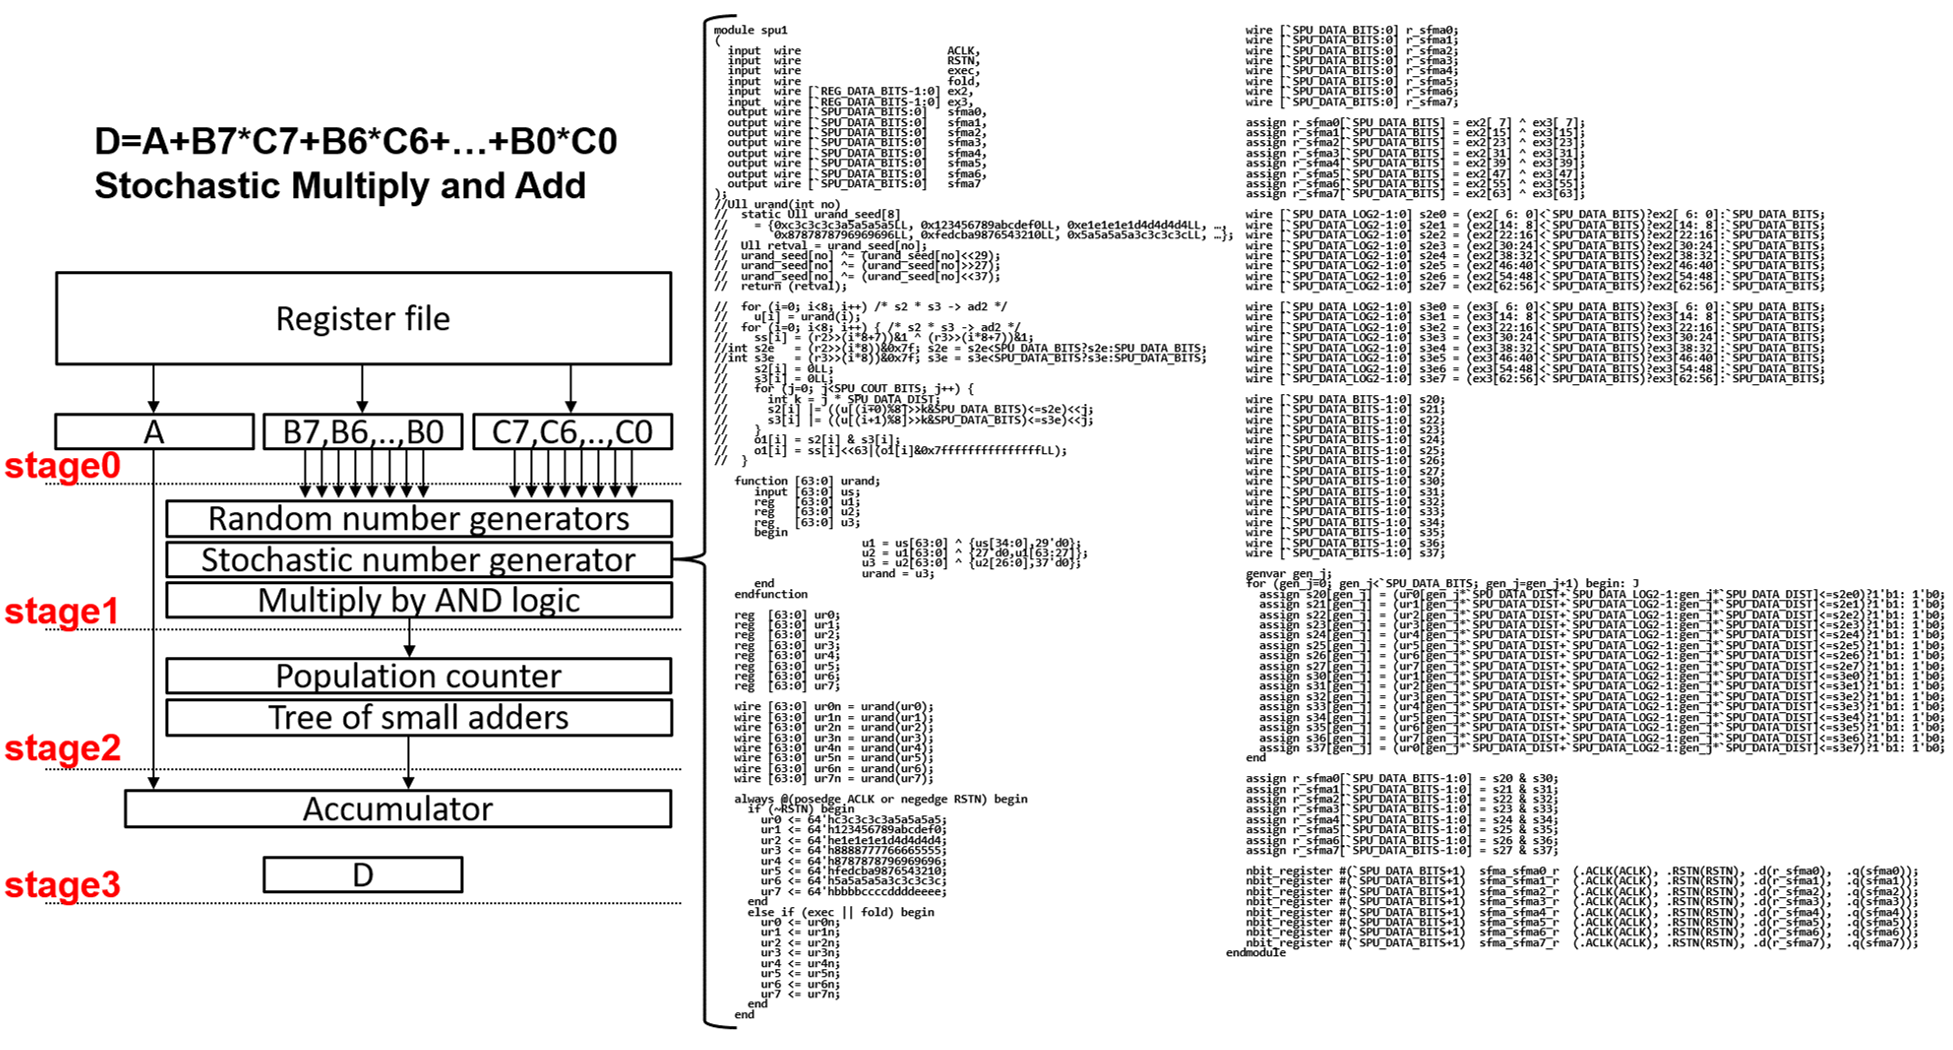
\includegraphics[angle=270,origin=b,width=1.00\textwidth]{sfma1.eps}
\caption{SFMA 1st stage}
\end{figure}

\begin{figure}[htbp]
\center
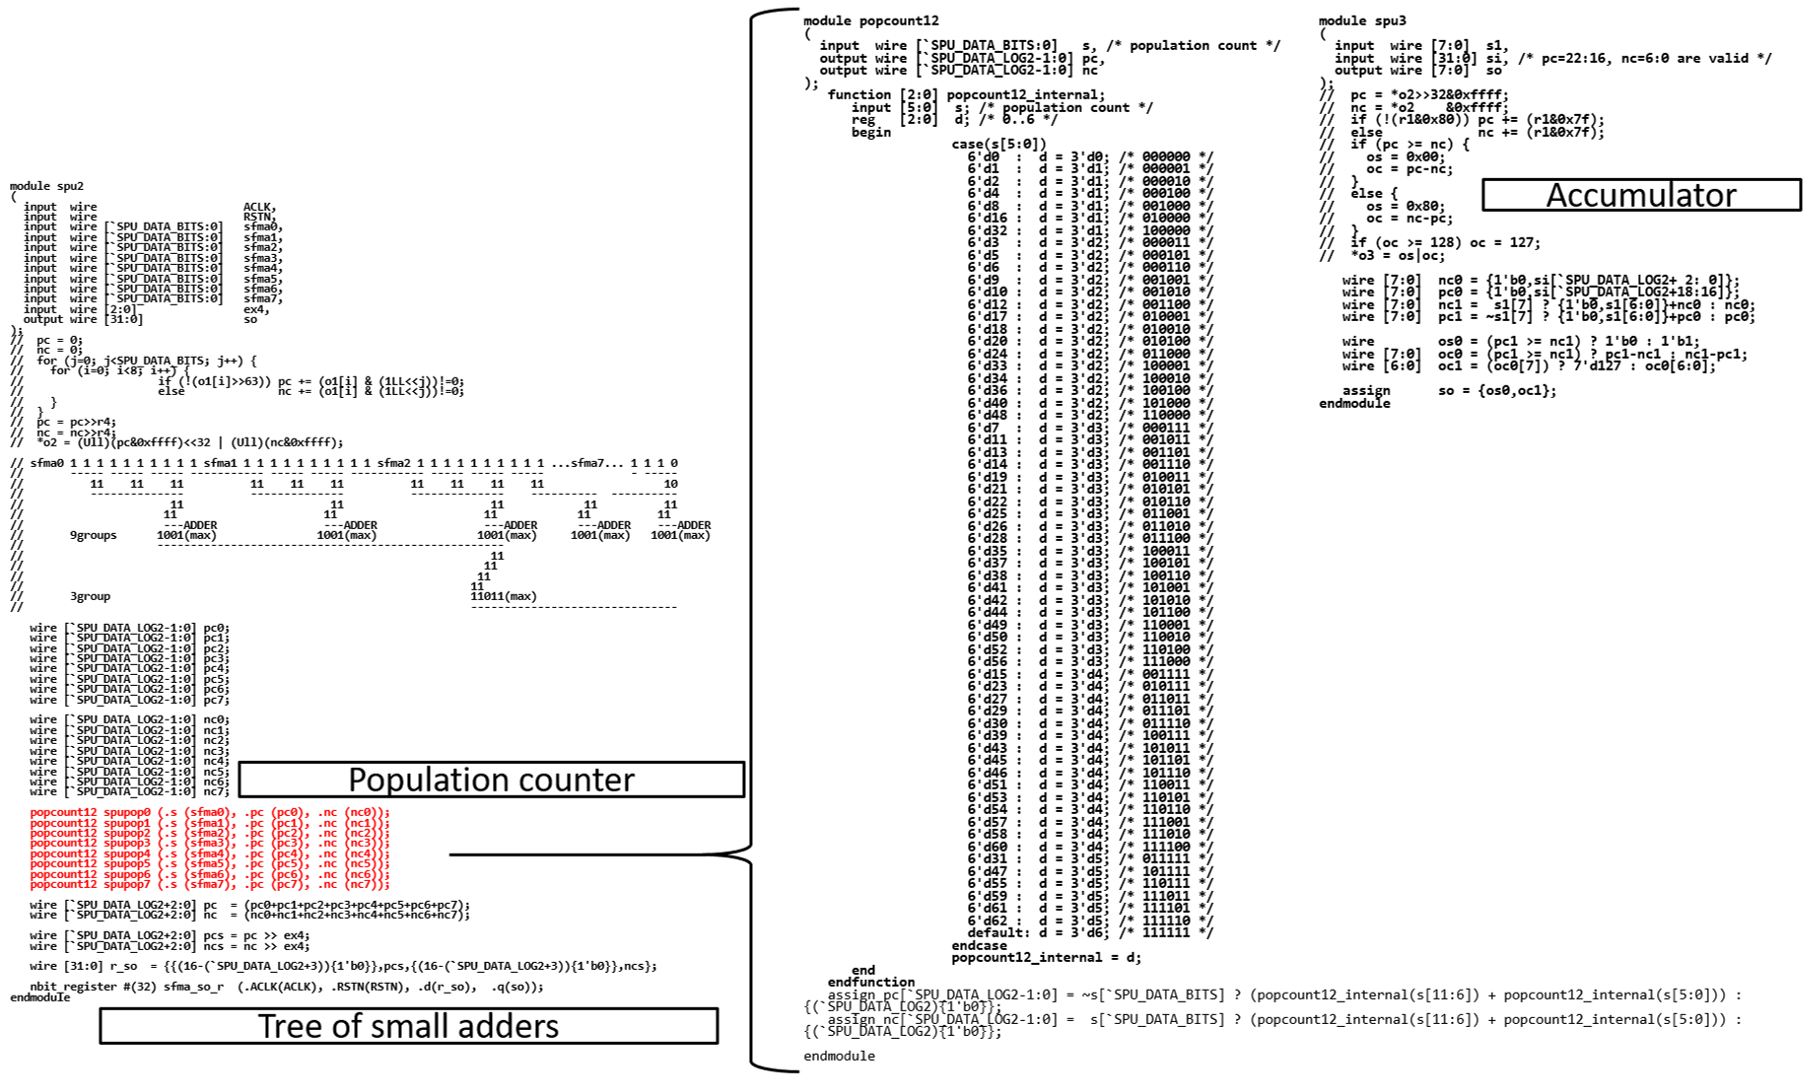
\includegraphics[angle=270,origin=b,width=1.00\textwidth]{sfma2.eps}
\caption{SFMA 2nd and 3rd stage}
\end{figure}

\clearpage

\subsection{Sparse matrix multiplication}

\shabox{
\leftline{cent\% make -f Makefile-csim.emax6+dma test022-csim.emax6+dma clean}
\leftline{cent\% ../../src/csim/csim -x test022-csim.emax6+dma}
}

\shabox{
\leftline{zynq\% make -f Makefile-zynq.emax6+dma test022-zynq.emax6+dma clean}
\leftline{zynq\% ./test022-zynq.emax6+dma}
}

\begin{figure}[htbp]
\center
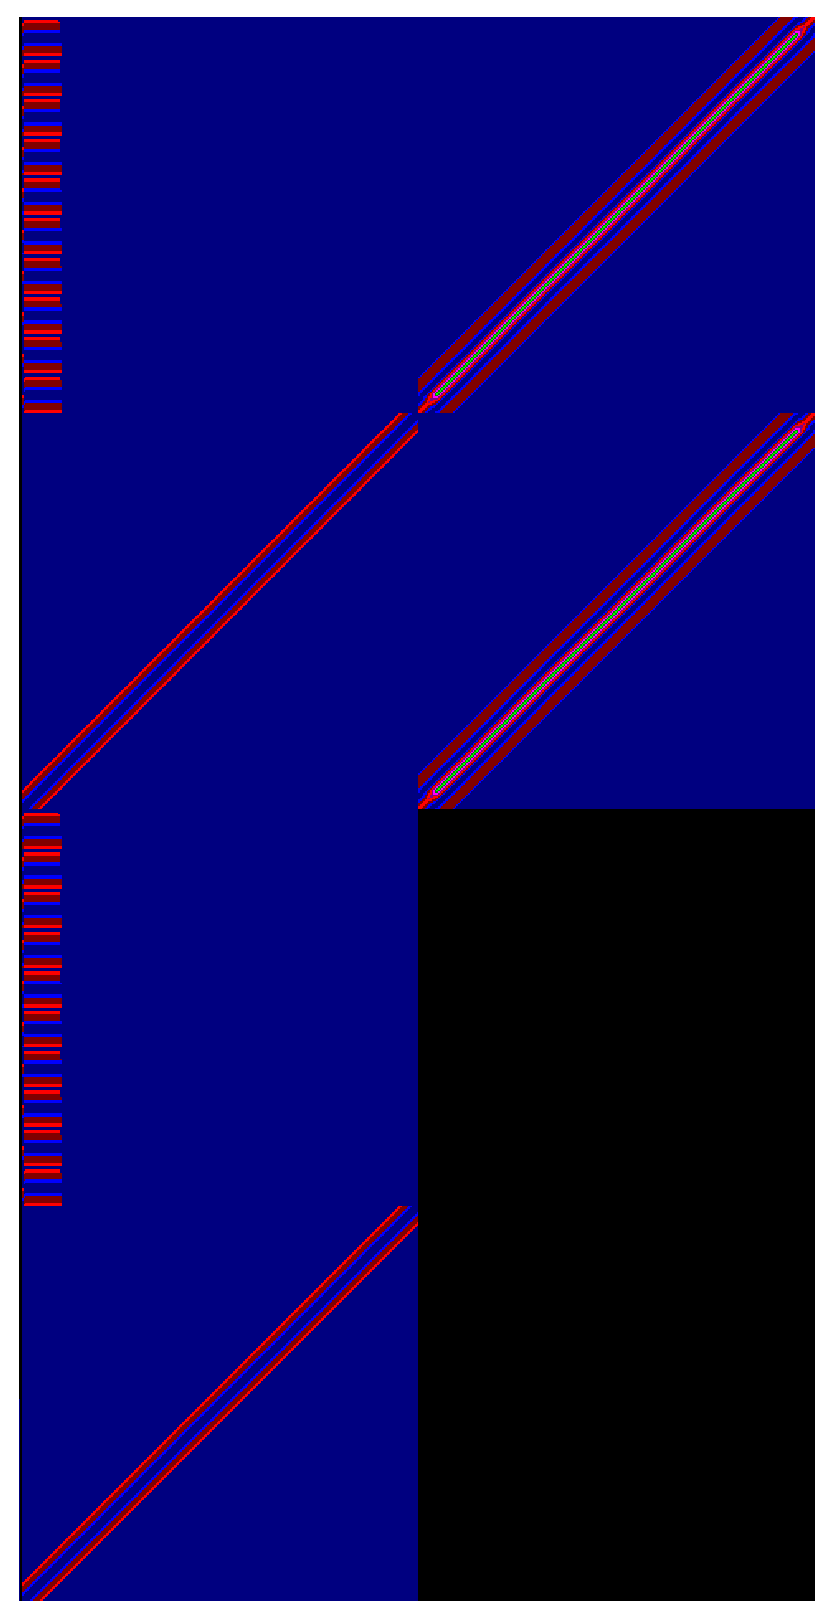
\includegraphics[angle=270,origin=b,width=0.75\textwidth]{sparse_mat.eps}
\caption{Sparse matrix multiplication}
\end{figure}

\subsubsection{Single flow}

\begin{screen}
\tiny
\begin{verbatim}
for (blk=0; blk<M2; blk+=RMGRP) { /* 3�ť롼��Ÿ���γ�¦�о� */
  for (top=0; top<M1/NCHIP; top+=H) { /* will be parallelized by multi-chip (M/#chip) */
    packed *a[H][NCHIP], *a0[H][NCHIP];
    packed *b, *b0[H];
    float  *c[H][NCHIP], *c0[H][NCHIP];
    b = B32_P+blk*LP;
    for (CHIP=0; CHIP<NCHIP; CHIP++) { /* will be parallelized by multi-chip (M/#chip) */
      for (k=0; k<H; k++) {
        a[k][CHIP]  = A32_P+(CHIP*M1/NCHIP+top+k)*LP;
        c[k][CHIP]  = C32_1+(CHIP*M1/NCHIP+top+k)*M2+blk;
        c0[k][CHIP] = c[k][CHIP]+0;
      }
    }

#define sparse_core1(r, h) \
  mex(OP_CMPA_LE,  &b0[h], INIT0?b:b0[h], INIT0?0:8, OP_CMPA_GE, &a0[h][CHIP], INIT0?a[h][CHIP]:a0[h][CHIP], INIT0?0:8, 0LL, BR[r][2][1], BR[r][2][0]);\
  mop(OP_LDR,   3, &BR[r][2][1], b0[h],                        bofs,        MSK_W1,      b,          2*LP*RMGRP,  0, 0,      NULL,      2*LP*RMGRP);/*LMM[2] col2*/\
  mop(OP_LDR,   3, &BR[r][2][0], a0[h][CHIP],                  bofs,        MSK_W0,      a[h][CHIP], 2*LP,        0, 0,      NULL,      2*LP);      /*LMM[1] col2*/\
  exe(OP_NOP,      &AR[r][0],    0LL,                          EXP_H3210,   0,           EXP_H3210,  0,           EXP_H3210, OP_NOP, 0, OP_NOP, 0);\
  mop(OP_LDWR,  1, &c00,         c0[h][CHIP],                  oofs,        MSK_W0,      c[h][CHIP], RMGRP,       0, 1,      NULL,      RMGRP);\
  exe(OP_CFMA,     &c00,         INIT0?c00:c00,                EXP_H3210,   BR[r][2][1], EXP_H3210,  BR[r][2][0], EXP_H3210, OP_NOP, 0, OP_NOP, 0);\
  mop(OP_STWR,  1, &c00,         oofs,                         c0[h][CHIP], MSK_D0,      c[h][CHIP], RMGRP,       0, 1,      NULL,      RMGRP)

//EMAX5A begin imax mapdist=0
/**/for (CHIP=0; CHIP<NCHIP; CHIP++) { /* will be parallelized by multi-chip (M/#chip) */
/*2*/ for (INIT1=1,LOOP1=RMGRP,rofs=(0-LP*8)<<32|((0-4LL)&0xffffffff); LOOP1--; INIT1=0) { /* stage#0 *//* mapped to FOR() on BR[63][1][0] */
  /*1*/ for (INIT0=1,LOOP0=LP,cofs=(0LL)<<32|((0LL)&0xffffffff); LOOP0--; INIT0=0) {         /* stage#0 *//* mapped to FOR() on BR[63][0][0] */
          exe(OP_ADD,    &rofs, rofs, EXP_H3210, INIT0?(LP*8)<<32|(4LL):0, EXP_H3210, 0LL, EXP_H3210, OP_NOP, 0LL,                  OP_NOP, 0LL); /* stage#0 */
          exe(OP_ADD,    &bofs, rofs, EXP_H3210, 0LL,                      EXP_H3210, 0LL, EXP_H3210, OP_AND, 0xffffffff00000000LL, OP_NOP, 0LL); /* stage#1 */
          exe(OP_ADD,    &oofs, rofs, EXP_H3210, 0LL,                      EXP_H3210, 0LL, EXP_H3210, OP_AND, 0x00000000ffffffffLL, OP_NOP, 0LL); /* stage#1 */

          sparse_core1(  2,  0);
          sparse_core1(  3,  1);
          sparse_core1(  4,  2);
          sparse_core1(  5,  3);
          sparse_core1(  6,  4);
          sparse_core1(  7,  5);
          sparse_core1(  8,  6);
          sparse_core1(  9,  7);
          sparse_core1( 10,  8);
          sparse_core1( 11,  9);
          sparse_core1( 12, 10);
          sparse_core1( 13, 11);
          sparse_core1( 14, 12);
          sparse_core1( 15, 13);
          sparse_core1( 16, 14);
          sparse_core1( 17, 15); /* H=16 */
        }
      }
    }
//EMAX5A end
  }
}
//EMAX5A drain_dirty_lmm
\end{verbatim}
\end{screen}

\begin{figure}[htbp]
\center
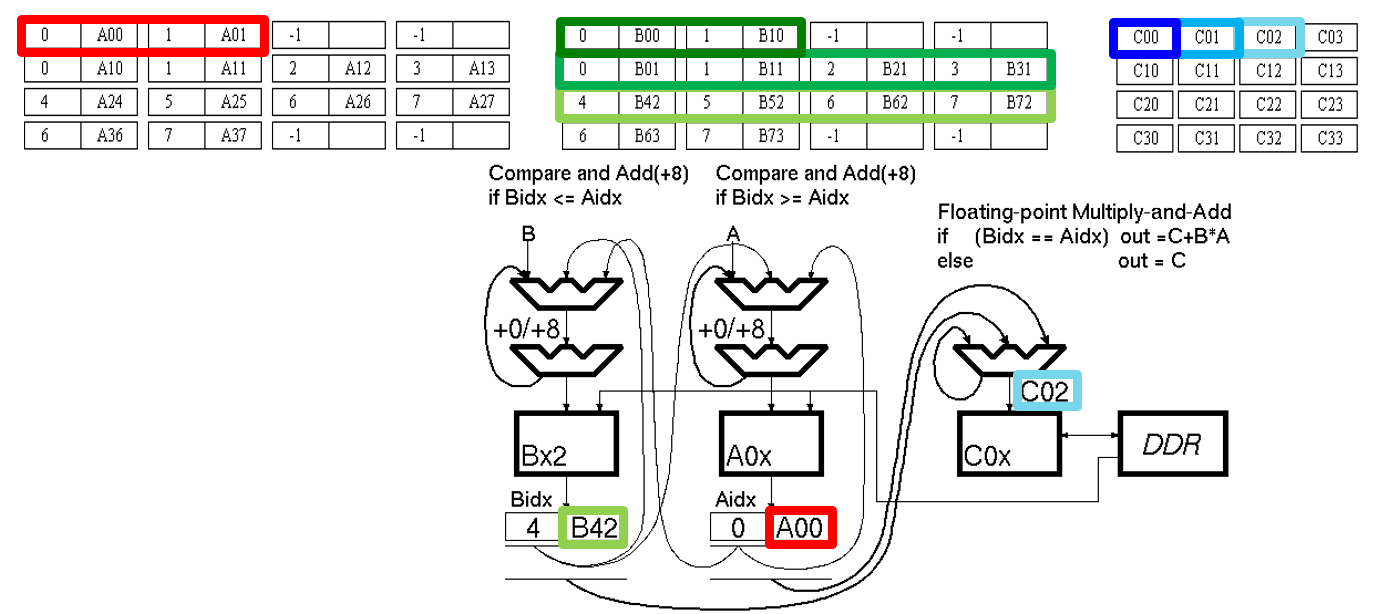
\includegraphics[angle=270,origin=b,width=1.00\textwidth]{SPMM.eps}
\caption{Data path for sparse matrix multiplication}
\end{figure}

\begin{figure}[htbp]
\center
\epsfile{file=EMAX6PIP.eps,width=1.00\textwidth}
\caption{Timing chart (single flow)}
\end{figure}

\begin{figure}[htbp]
\center
\epsfile{file=test022-imax-emax6.eps,width=1.00\textwidth}
\caption{Sparse matrix multiplication (single flow)}
\end{figure}

\clearpage

\subsubsection{Dual flow}

\begin{screen}
\tiny
\begin{verbatim}
  for (blk=0; blk<M2; blk+=RMGRP) { /* 3�ť롼��Ÿ���γ�¦�о� */
    for (top=0; top<M1/NCHIP; top+=H) { /* will be parallelized by multi-chip (M/#chip) */
      packed *a[H][NCHIP], *a0[H][2][NCHIP]; /* a�϶���,a0��Ʊ��Ԥ򻲾�(��ư�ѥ����󤬰㤦�Τ�2��ɬ��) */
      packed *b[2],        *b0[H][2];        /* b�϶���,b0��2�Ԥ�1unit�˥ޥ������åɲ������c��Ϣ³ */
      float  *c[H][NCHIP], *c0[H][2][NCHIP]; /* c�϶���,c0��Ϣ³ */
      b[0] = B32_P+(blk+0)*LP;
      b[1] = B32_P+(blk+1)*LP;
      for (CHIP=0; CHIP<NCHIP; CHIP++) { /* will be parallelized by multi-chip (M/#chip) */
        for (k=0; k<H; k++) {
          a[k][CHIP]  = A32_P+(CHIP*M1/NCHIP+top+k)*LP;
          c[k][CHIP]  = C32_1+(CHIP*M1/NCHIP+top+k)*M2+blk;
          c0[k][0][CHIP] = c[k][CHIP]+0;
          c0[k][1][CHIP] = c[k][CHIP]+1;
      } }
#define sparse_core1(r, h) \
  mex(OP_CMPA_LE, &b0[h][0], INIT0?b[0]:b0[h][0], INIT0?0:8, OP_CMPA_GE, &a0[h][0][CHIP], INIT0?a[h][CHIP]:a0[h][0][CHIP], INIT0?0:8, 0LL, BR[r][2][1], BR[r][2][0]);\
  mop(OP_LDR,   3, &BR[r][2][1],    b0[h][0],                        bofs,           MSK_W1,      b[0],          2*LP*RMGRP,  0, 0,      NULL,      2*LP*RMGRP);\
  mop(OP_LDR,   3, &BR[r][2][0],    a0[h][0][CHIP],                  bofs,           MSK_W0,      a[h][CHIP],    2*LP,        0, 0,      NULL,      2*LP);\
  mex(OP_CMPA_LE, &b0[h][1], INIT0?b[1]:b0[h][1], INIT0?0:8, OP_CMPA_GE, &a0[h][1][CHIP], INIT0?a[h][CHIP]:a0[h][1][CHIP], INIT0?0:8, 0LL, BR[r][3][1], BR[r][3][0]);\
  mop(OP_LDR,   3, &BR[r][3][1],    b0[h][1],                        bofs,           MSK_W1,      b[0],          2*LP*RMGRP,  0, 0,      NULL,      2*LP*RMGRP);\
  mop(OP_LDR,   3, &BR[r][3][0],    a0[h][1][CHIP],                  bofs,           MSK_W0,      a[h][CHIP],    2*LP,        0, 0,      NULL,      2*LP);\
  exe(OP_NOP,      &AR[r][0],       0LL,                             EXP_H3210,      0,           EXP_H3210,     0,           EXP_H3210, OP_NOP, 0, OP_NOP, 0);\
  mop(OP_LDWR,  1, &c00,            c0[h][0][CHIP],                  oofs,           MSK_W0,      c[h][CHIP],    RMGRP,       0, 1,      NULL,      RMGRP);\
  exe(OP_CFMA,     &c00,            INIT0?c00:c00,                   EXP_H3210,      BR[r][2][1], EXP_H3210,     BR[r][2][0], EXP_H3210, OP_NOP, 0, OP_NOP, 0);\
  mop(OP_STWR,  1, &c00,            oofs,                            c0[h][0][CHIP], MSK_D0,      c[h][CHIP],    RMGRP,       0, 1,      NULL,      RMGRP);\
  mop(OP_LDWR,  1, &c01,            c0[h][1][CHIP],                  oofs,           MSK_W0,      c[h][CHIP],    RMGRP,       0, 1,      NULL,      RMGRP);\
  exe(OP_CFMA,     &c01,            INIT0?c01:c01,                   EXP_H3210,      BR[r][3][1], EXP_H3210,     BR[r][3][0], EXP_H3210, OP_NOP, 0, OP_NOP, 0);\
  mop(OP_STWR,  1, &c01,            oofs,                            c0[h][1][CHIP], MSK_D0,      c[h][CHIP],    RMGRP,       0, 1,      NULL,      RMGRP)
//EMAX5A begin imax mapdist=0
/*3*/ for (CHIP=0; CHIP<NCHIP; CHIP++) { /* will be parallelized by multi-chip (M/#chip) */
  /*2*/ for (INIT1=1,LOOP1=RMGRP/2,rofs=(0-8*LP*2)<<32|((0-8LL)&0xffffffff); LOOP1--; INIT1=0) { /* stage#0 *//* mapped to FOR() on BR[63][1][0] */
    /*1*/ for (INIT0=1,LOOP0=LP,cofs=(0LL)<<32|((0LL)&0xffffffff); LOOP0--; INIT0=0) {         /* stage#0 *//* mapped to FOR() on BR[63][0][0] */
            exe(OP_ADD,    &rofs, rofs,            EXP_H3210, INIT0?(8*LP*2)<<32|(8LL):0, EXP_H3210, 0LL, EXP_H3210, OP_NOP, 0LL,                  OP_NOP, 0LL);
            exe(OP_ADD,    &bofs, rofs,            EXP_H3210, 0LL,                        EXP_H3210, 0LL, EXP_H3210, OP_AND, 0xffffffff00000000LL, OP_NOP, 0LL);
            exe(OP_ADD,    &oofs, rofs,            EXP_H3210, 0LL,                        EXP_H3210, 0LL, EXP_H3210, OP_AND, 0x00000000ffffffffLL, OP_NOP, 0LL);
            sparse_core1(  2,  0);
            sparse_core1(  3,  1); /* H=2 */
            sparse_core1(  4,  2);
            sparse_core1(  5,  3); /* H=4 */
            sparse_core1(  6,  4);
            sparse_core1(  7,  5);
            sparse_core1(  8,  6);
            sparse_core1(  9,  7); /* H=8 */
            sparse_core1( 10,  8);
            sparse_core1( 11,  9);
            sparse_core1( 12, 10);
            sparse_core1( 13, 11);
            sparse_core1( 14, 12);
            sparse_core1( 15, 13);
            sparse_core1( 16, 14);
            sparse_core1( 17, 15); /* H=16 */
      } } }
//EMAX5A end
  } }
//EMAX5A drain_dirty_lmm
\end{verbatim}
\end{screen}

\begin{figure}[htbp]
\center
\epsfile{file=EMAX6PIP2.eps,width=1.00\textwidth}
\caption{Timing chart (dual flow)}
\end{figure}

\begin{figure}[htbp]
\center
\epsfile{file=test022-imax-emax62.eps,width=1.00\textwidth}
\caption{Sparse matrix multiplication (dual flow)}
\end{figure}

\clearpage

\subsection{Sparse matrix compression}

\shabox{
\leftline{cent\% make -f Makefile-csim.emax6+dma test024-csim.emax6+dma clean}
\leftline{cent\% ../../src/csim/csim -x test024-csim.emax6+dma}
}

\shabox{
\leftline{zynq\% make -f Makefile-zynq.emax6+dma test024-zynq.emax6+dma clean}
\leftline{zynq\% ./test024-zynq.emax6+dma}
}

\vskip .1in

̩������¹��󰵽�ɽ�����Ѵ����롥mapdist=0�Τޤޡ�Ʊ��LMM����Ⱦ�ȸ�Ⱦ����
�˻Ȥäơ����֥�Хåե���󥰤��롥����¹Է�̤�drain�ȡ����̱黻�ȡ�����
�¹Ԥ�ɬ�פ�̩����Υ����ɤ�Ʊ���˼¹Ԥ��뤳�Ȥǡ���®�����Ƥ��롥mop()���
f=1�ˤ��뤳�Ȥǡ�BasIP������DDR�ؤν��ᤷ���������Ƥ���(�ǽ��1�����
load��������Τϻ����ʤ�)��

\begin{screen}
\tiny
\begin{verbatim}
  *Bas1P = B32_P-1; /* end of B32_0 */
  for (i=0; i<M1; i+=RMGRP) {
    r1     = (Ull)(i*M2-1)<<32;
    ibase0 = B32_0+i*M2;
    itop0  = B32_0+i*M2;
    itop1  = itop0+RMGRP*M2;
    obase0 = *Bas1P;   /* end of B32_0 */
    otop1  = otop0;
    otop0  = *Bas1P+8; /* top of B32_P */

//with-prefetch/post-drain
//EMAX5A begin imax mapdist=0
/*3*/for (CHIP=0; CHIP<NCHIP; CHIP++) {
  /*2*/for (INIT1=1,LOOP1=RMGRP,rofs=0; LOOP1--; INIT1=0) {
    /*1*/for (INIT0=1,LOOP0=M2,cofs=0; LOOP0--; INIT0=0) {
           mop(OP_LDWR, 1,   &r0,       ibase0++,          0,             MSK_D0,    itop0, M2*RMGRP,    0,       0,    itop1,  M2*RMGRP);
           exe(OP_ADD,       &r1,       r1,     EXP_H3210, 0x100000000LL, EXP_H3210, 0,     EXP_H3210,   OP_NOP,  0,    OP_NOP, 0LL);
           exe(OP_NOP,       &std,      r1,     EXP_H3210, 0,             EXP_H3210, 0,     EXP_H3210,   OP_OR,   r0,   OP_NOP, 0LL);
           exe(OP_CMP_EQ,    &cc0,      r0,     EXP_H1010, 0x00000000LL,  EXP_H1010, 0,     EXP_H3210,   OP_NOP,  0,    OP_NOP, 0LL);
           exe(OP_CMP_EQ,    &cc1,      r0,     EXP_H1010, 0x80000000LL,  EXP_H1010, 0,     EXP_H3210,   OP_NOP,  0,    OP_NOP, 0LL);
           exe(OP_NOP,       &cc2,      cc0,    EXP_H3210, 0,             EXP_H3210, 0,     EXP_H1010,   OP_OR,   cc1,  OP_NOP, 0LL);
           exe(OP_CMOV,      &oofs,     cc2,    EXP_H3210, 0,             EXP_H3210, 8,     EXP_H3210,   OP_NOP,  0,    OP_NOP, 0LL);
           exe(OP_ADD,       &obase0,   obase0, EXP_H3210, oofs,          EXP_H3210, 0,     EXP_H3210,   OP_NOP,  0,    OP_NOP, 0LL);
           mop(OP_STR,  3,   &obase0,   Bas1P,             0,             MSK_D0,    Bas1P, 2,           0,       0,    NULL,   2);
           exe(OP_NOP,       &AR[5][0], 0,   EXP_H3210,    0,             EXP_H3210, 0,     EXP_H1010,   OP_NOP,  0,    OP_NOP, 0LL);
           cex(OP_CEXE,      &ex0,      0, 0, 0, cc2, 0x0001);
           mop(OP_STR,  ex0, &std,      obase0,            0,             MSK_D0,    otop0, LP*2*RMGRP,  0,       0,    otop1,  LP*2*RMGRP);
         }
       }
     }
//EMAX5A end
//EMAX5A drain_dirty_lmm
  }
  count1 = (packed*)*Bas1P-(packed*)B32_P+1;
  printf("Bas1P=%08.8x_%08.8x Packed=%d\n", (Uint)(*Bas1P>>32), (Uint)*Bas1P, count1);
\end{verbatim}
\end{screen}

\begin{figure}[htbp]
\center
\epsfile{file=test024-imax-emax6.eps,width=1.00\textwidth}
\caption{Sparse matrix compression}
\end{figure}

\clearpage

\section{2D-imaging}

\shabox{
\leftline{cent\% make -f Makefile-csim.emax6+dma all clean}
\leftline{cent\% ../../src/csim/csim -x filter-csim.emax6+dma -f 81.ppm 82.ppm}
}

\shabox{
\leftline{zynq\% make -f Makefile-zynq.emax6+dma all clean}
\leftline{zynq\% ./filter-zynq.emax6+dma -f 81.ppm 82.ppm}
}

\subsection{Tone\_curve}

\begin{figure}[htbp]
\center
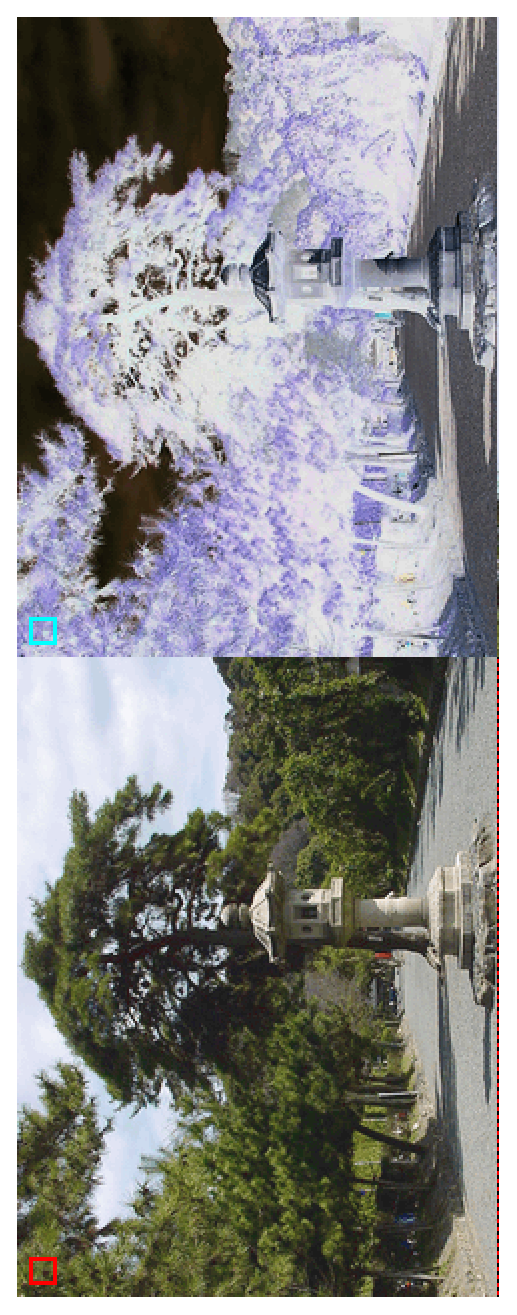
\includegraphics[angle=270,origin=b,width=0.75\textwidth]{tone_curve.eps}
\caption{Tone curve}
\end{figure}

RGB�ƿ����Ѵ��ơ��֥�˴�Ť����������Ѵ����롥���٤ΥС����ȱ黻�ˤ�ꡤ
10�ս��OMAP=10�ˤγơ��ˤĤ��ơ�6��ʬ�α黻��Ԥ���RMGRP=6�ˡ����ƥ󥷥��
���ǤϤʤ�����mapdist=0�Ǥ��롥�ʤ���̤����stage����Ѥ���PLOAD�ˤ����ǽ��
�夬��ǽ�Ǥ��롥

\begin{screen}
\tiny
\begin{verbatim}
void tone_curve(Uint *r, Uint *d, Uchar *t) /* R, D, lut */
#if !defined(EMAX5) && !defined(EMAX6)
  for (top=PAD; top<HT-PAD; top++) { /* will be parallelized by multi-chip (M/#chip) */
    for (cofs=PAD; cofs<WD-PAD; cofs++) {
      Uint pix = *(r+top*WD+cofs);
      *(d+top*WD+cofs) = ((t)[pix>>24])<<24 | (t[256+((pix>>16)&255)])<<16 | (t[512+((pix>>8)&255)])<<8;
    }
  }
#endif
\end{verbatim}
\end{screen}

\begin{screen}
\tiny
\begin{verbatim}
  for (top=0; top<RRANGE; top+=RMGRP) { /* will be parallelized by multi-chip (M/#chip) */
    for (CHIP=0; CHIP<NCHIP; CHIP++) { /* will be parallelized by multi-chip (M/#chip) */
      for (rofs=0; rofs<RMGRP; rofs++) { /* will be parallelized by multi-chip (M/#chip) */
        int idx = (CHIP*RRANGE*OMAP+top+rofs)*WD;
        for (cofs=PAD; cofs<WD-PAD; cofs++) {
          for (oc=0; oc<OMAP; oc++) {
            Uint pix = *(r+idx+oc*RRANGE*WD+cofs);
            *(d+idx+oc*RRANGE*WD+cofs) = ((t)[pix>>24])<<24 | (t[256+((pix>>16)&255)])<<16 | (t[512+((pix>>8)&255)])<<8;
          }
        }
      }
    }
  }
\end{verbatim}
\end{screen}

\begin{screen}
\tiny
\begin{verbatim}
  Ull  LOOP1, LOOP0;
  Ull  INIT1, INIT0;
  Ull  AR[64][4];                     /* output of EX     in each unit */
  Ull  BR[64][4][4];                  /* output registers in each unit */
  Ull  r0, r1, r2, r3, r4, r5, r6, r7, r8, r9, r10, r11, r12, r13, r14, r15;
  Ull  r16, r17, r18, r19, r20, r21, r22, r23, r24, r25, r26, r27, r28, r29, r30, r31;
  Ull  cc0, cc1, cc2, cc3, ex0, ex1;
  for (top=0; top<RRANGE; top+=RMGRP) {
    Ull  rtop0[NCHIP], dtop0[NCHIP];
    Ull  rtop1[NCHIP], dtop1[NCHIP];
    Ull  rtop2[NCHIP], dtop2[NCHIP];
    Ull  rtop3[NCHIP], dtop3[NCHIP];
    Ull  rtop4[NCHIP], dtop4[NCHIP];
    Ull  rtop5[NCHIP], dtop5[NCHIP];
    Ull  rtop6[NCHIP], dtop6[NCHIP];
    Ull  rtop7[NCHIP], dtop7[NCHIP];
    Ull  rtop8[NCHIP], dtop8[NCHIP];
    Ull  rtop9[NCHIP], dtop9[NCHIP];
    for (CHIP=0; CHIP<NCHIP; CHIP++) { /* output channels are parallelized by multi-chip (OC/#chip) */
      rtop0[CHIP] = r+(CHIP*RRANGE*OMAP+RRANGE*0+top)*WD; dtop0[CHIP] = d+(CHIP*RRANGE*OMAP+RRANGE*0+top)*WD;
        :
      rtop9[CHIP] = r+(CHIP*RRANGE*OMAP+RRANGE*9+top)*WD; dtop9[CHIP] = d+(CHIP*RRANGE*OMAP+RRANGE*9+top)*WD;
    }
//EMAX5A begin tone_curve mapdist=0
    for (CHIP=0; CHIP<NCHIP; CHIP++) { /* output channels are parallelized by multi-chip (OC/#chip) */
 /*2*/for (INIT1=1,LOOP1=RMGRP,rofs=0-WD*4; LOOP1--; INIT1=0) {      /* stage#0 *//* mapped to FOR() on BR[63][1][0] */
   /*1*/for (INIT0=1,LOOP0=WD,cofs=0-4; LOOP0--; INIT0=0) {          /* stage#0 *//* mapped to FOR() on BR[63][0][0] */
          exe(OP_ADD,  &cofs, INIT0?cofs:cofs, EXP_H3210, 4, EXP_H3210, 0LL, EXP_H3210, OP_AND, 0x00000000ffffffffLL, OP_NOP, 0LL);  /* stage#0 */
          exe(OP_ADD,  &rofs, rofs, EXP_H3210, INIT0?WD*4:0, EXP_H3210, 0LL, EXP_H3210, OP_NOP, 0LL, OP_NOP, 0LL);                   /* stage#0 */
          exe(OP_ADD,  &pofs, rofs, EXP_H3210, cofs, EXP_H3210, 0LL, EXP_H3210, OP_AND, 0x00000000ffffffffLL, OP_NOP, 0LL);          /* stage#1 */
          /*map0*/
          mop(OP_LDWR,  1, &BR[2][1][1], (Ull)rtop0[CHIP], pofs,  MSK_D0, (Ull)rtop0[CHIP], WD*RMGRP, 0, 0, (Ull)NULL, WD*RMGRP);    /* stage#2 */
          mop(OP_LDBR,  1, &BR[3][1][1], (Ull)t1,    BR[2][1][1], MSK_B3, (Ull)t1, 256/4,  0,  0, (Ull)NULL, 256/4);                 /* stage#3 */
          mop(OP_LDBR,  1, &BR[3][2][1], (Ull)t2,    BR[2][1][1], MSK_B2, (Ull)t2, 256/4,  0,  0, (Ull)NULL, 256/4);                 /* stage#3 */
          mop(OP_LDBR,  1, &BR[3][3][1], (Ull)t3,    BR[2][1][1], MSK_B1, (Ull)t3, 256/4,  0,  0, (Ull)NULL, 256/4);                 /* stage#3 */
          exe(OP_MMRG, &r1, BR[3][1][1], EXP_H3210,  BR[3][2][1], EXP_H3210, BR[3][3][1], EXP_H3210, OP_NOP, 0LL, OP_NOP, 0LL);      /* stage#3 */
          mop(OP_STWR,  3, &r1,          (Ull)dtop0[CHIP], pofs,  MSK_D0, (Ull)dtop0[CHIP], WD*RMGRP, 0, 0, (Ull)NULL, WD*RMGRP);    /* stage#3 */
             :
          /*map5*/
          mop(OP_LDWR,  1, &BR[12][1][1],(Ull)rtop5[CHIP], pofs,  MSK_D0, (Ull)rtop5[CHIP], WD*RMGRP, 0, 0, (Ull)NULL, WD*RMGRP);    /* stage#12 */
          mop(OP_LDBR,  1, &BR[13][1][1],(Ull)t1,    BR[12][1][1],MSK_B3, (Ull)t1, 256/4,  0,  0, (Ull)NULL, 256/4);                 /* stage#13 */
          mop(OP_LDBR,  1, &BR[13][2][1],(Ull)t2,    BR[12][1][1],MSK_B2, (Ull)t2, 256/4,  0,  0, (Ull)NULL, 256/4);                 /* stage#13 */
          mop(OP_LDBR,  1, &BR[13][3][1],(Ull)t3,    BR[12][1][1],MSK_B1, (Ull)t3, 256/4,  0,  0, (Ull)NULL, 256/4);                 /* stage#13 */
          exe(OP_MMRG, &r1, BR[13][1][1],EXP_H3210,  BR[13][2][1],EXP_H3210, BR[13][3][1],EXP_H3210, OP_NOP, 0LL, OP_NOP, 0LL);      /* stage#13 */
          mop(OP_STWR,  3, &r1,          (Ull)dtop5[CHIP], pofs,  MSK_D0, (Ull)dtop5[CHIP], WD*RMGRP, 0, 0, (Ull)NULL, WD*RMGRP);    /* stage#13 */
          /*map6*/
          mop(OP_LDWR,  1, &BR[14][1][1],(Ull)rtop6[CHIP], pofs,  MSK_D0, (Ull)rtop6[CHIP], WD*RMGRP, 0, 0, (Ull)NULL, WD*RMGRP);    /* stage#14 */
          mop(OP_LDBR,  1, &BR[15][1][1],(Ull)t1,    BR[14][1][1],MSK_B3, (Ull)t1, 256/4,  0,  0, (Ull)NULL, 256/4);                 /* stage#15 */
          mop(OP_LDBR,  1, &BR[15][2][1],(Ull)t2,    BR[14][1][1],MSK_B2, (Ull)t2, 256/4,  0,  0, (Ull)NULL, 256/4);                 /* stage#15 */
          mop(OP_LDBR,  1, &BR[15][3][1],(Ull)t3,    BR[14][1][1],MSK_B1, (Ull)t3, 256/4,  0,  0, (Ull)NULL, 256/4);                 /* stage#15 */
          exe(OP_MMRG, &r1, BR[15][1][1],EXP_H3210,  BR[15][2][1],EXP_H3210, BR[15][3][1],EXP_H3210, OP_NOP, 0LL, OP_NOP, 0LL);      /* stage#15 */
          mop(OP_STWR,  3, &r1,          (Ull)dtop6[CHIP], pofs,  MSK_D0, (Ull)dtop6[CHIP], WD*RMGRP, 0, 0, (Ull)NULL, WD*RMGRP);    /* stage#15 */
          /*map7*/
          mop(OP_LDWR,  1, &BR[16][1][1],(Ull)rtop7[CHIP], pofs,  MSK_D0, (Ull)rtop7[CHIP], WD*RMGRP, 0, 0, (Ull)NULL, WD*RMGRP);    /* stage#16 */
          mop(OP_LDBR,  1, &BR[17][1][1],(Ull)t1,    BR[16][1][1],MSK_B3, (Ull)t1, 256/4,  0,  0, (Ull)NULL, 256/4);                 /* stage#17 */
          mop(OP_LDBR,  1, &BR[17][2][1],(Ull)t2,    BR[16][1][1],MSK_B2, (Ull)t2, 256/4,  0,  0, (Ull)NULL, 256/4);                 /* stage#17 */
          mop(OP_LDBR,  1, &BR[17][3][1],(Ull)t3,    BR[16][1][1],MSK_B1, (Ull)t3, 256/4,  0,  0, (Ull)NULL, 256/4);                 /* stage#17 */
          exe(OP_MMRG, &r1, BR[17][1][1],EXP_H3210,  BR[17][2][1],EXP_H3210, BR[17][3][1],EXP_H3210, OP_NOP, 0LL, OP_NOP, 0LL);      /* stage#17 */
          mop(OP_STWR,  3, &r1,          (Ull)dtop7[CHIP], pofs,  MSK_D0, (Ull)dtop7[CHIP], WD*RMGRP, 0, 0, (Ull)NULL, WD*RMGRP);    /* stage#17 */
          /*map8*/
          mop(OP_LDWR,  1, &BR[18][1][1],(Ull)rtop8[CHIP], pofs,  MSK_D0, (Ull)rtop8[CHIP], WD*RMGRP, 0, 0, (Ull)NULL, WD*RMGRP);    /* stage#18 */
          mop(OP_LDBR,  1, &BR[19][1][1],(Ull)t1,    BR[18][1][1],MSK_B3, (Ull)t1, 256/4,  0,  0, (Ull)NULL, 256/4);                 /* stage#19 */
          mop(OP_LDBR,  1, &BR[19][2][1],(Ull)t2,    BR[18][1][1],MSK_B2, (Ull)t2, 256/4,  0,  0, (Ull)NULL, 256/4);                 /* stage#19 */
          mop(OP_LDBR,  1, &BR[19][3][1],(Ull)t3,    BR[18][1][1],MSK_B1, (Ull)t3, 256/4,  0,  0, (Ull)NULL, 256/4);                 /* stage#19 */
          exe(OP_MMRG, &r1, BR[19][1][1],EXP_H3210,  BR[19][2][1],EXP_H3210, BR[19][3][1],EXP_H3210, OP_NOP, 0LL, OP_NOP, 0LL);      /* stage#19 */
          mop(OP_STWR,  3, &r1,          (Ull)dtop8[CHIP], pofs,  MSK_D0, (Ull)dtop8[CHIP], WD*RMGRP, 0, 0, (Ull)NULL, WD*RMGRP);    /* stage#19 */
          /*map9*/
          mop(OP_LDWR,  1, &BR[20][1][1],(Ull)rtop9[CHIP], pofs,  MSK_D0, (Ull)rtop9[CHIP], WD*RMGRP, 0, 0, (Ull)NULL, WD*RMGRP);    /* stage#20 */
          mop(OP_LDBR,  1, &BR[21][1][1],(Ull)t1,    BR[20][1][1],MSK_B3, (Ull)t1, 256/4,  0,  0, (Ull)NULL, 256/4);                 /* stage#21 */
          mop(OP_LDBR,  1, &BR[21][2][1],(Ull)t2,    BR[20][1][1],MSK_B2, (Ull)t2, 256/4,  0,  0, (Ull)NULL, 256/4);                 /* stage#21 */
          mop(OP_LDBR,  1, &BR[21][3][1],(Ull)t3,    BR[20][1][1],MSK_B1, (Ull)t3, 256/4,  0,  0, (Ull)NULL, 256/4);                 /* stage#21 */
          exe(OP_MMRG, &r1, BR[21][1][1],EXP_H3210,  BR[21][2][1],EXP_H3210, BR[21][3][1],EXP_H3210, OP_NOP, 0LL, OP_NOP, 0LL);      /* stage#21 */
          mop(OP_STWR,  3, &r1,          (Ull)dtop9[CHIP], pofs,  MSK_D0, (Ull)dtop9[CHIP], WD*RMGRP, 0, 0, (Ull)NULL, WD*RMGRP);    /* stage#21 */
    } } }
//EMAX5A end
  }
//EMAX5A drain_dirty_lmm
\end{verbatim}
\end{screen}

\begin{figure}[htbp]
\center
\epsfile{file=filter+rmm-tone_curve-emax6.eps,width=1.00\textwidth}
\caption{Tone curve}
\end{figure}

\clearpage

\subsection{Hokan1 with stencil}

\begin{figure}[htbp]
\center
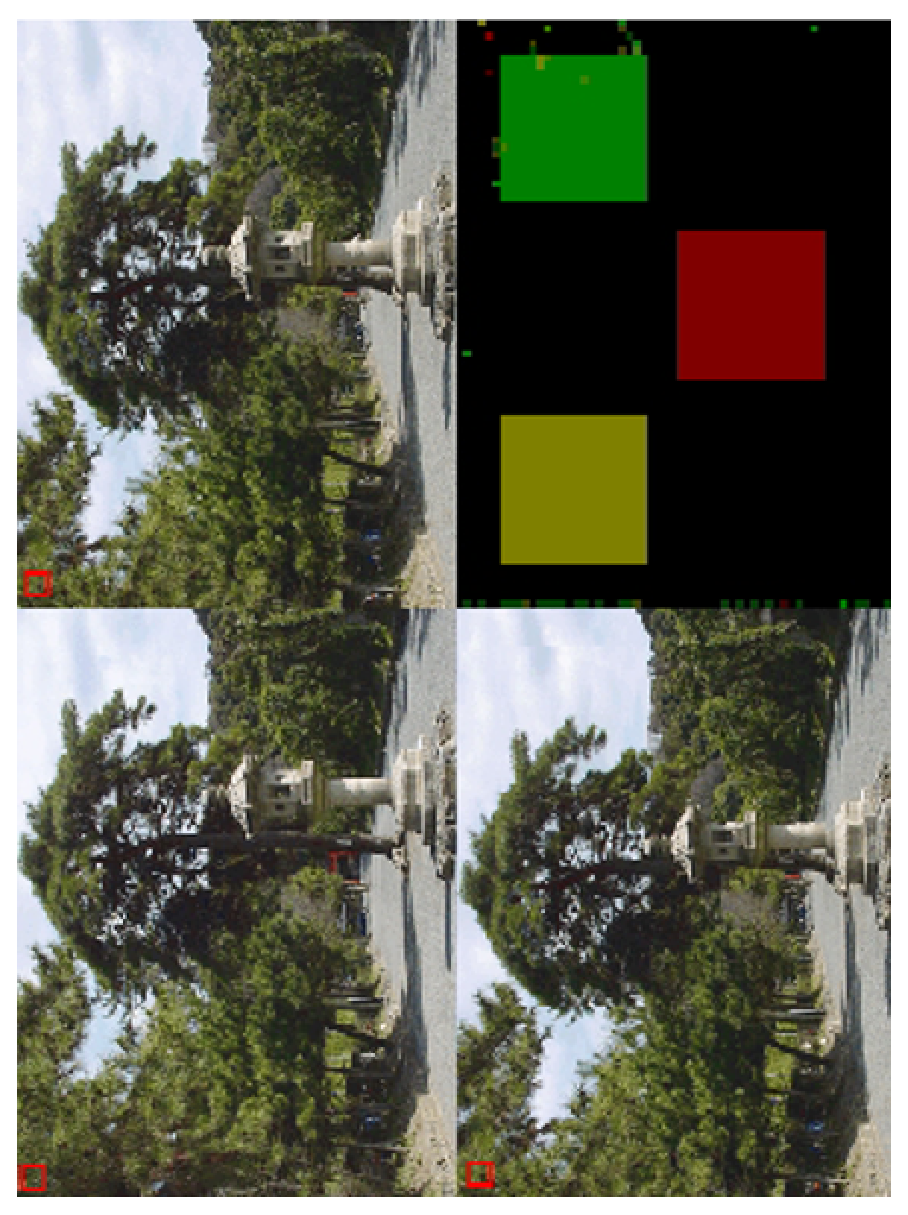
\includegraphics[angle=270,origin=b,width=0.50\textwidth]{hokan.eps}
\caption{Hokan}
\end{figure}

�ե졼����֤���1�ʳ��Ǥ��롥12x12���ΰ��4x4���ΰ��SAD�͡�4x4�ġˤ���롥
���٤ΥС����ȱ黻�ˤ��8��ʬ��SAD�׻���Ԥ���RMGRP=8�ˡ����ƥ󥷥�׻��Ǥ�
��mapdist=7�Ǥ��롥

\begin{screen}
\tiny
\begin{verbatim}
void hokan1(Uint *c, Uint *p, struct SAD1 *s) /* W, R, SAD1 */
#if !defined(EMAX5) && !defined(EMAX6)
  for (top=PAD; top<HT-PAD; top++) { /* scan-lines */
    for (pofs=-4; pofs<4; pofs++) {
      Ushort *t = s->SAD1[top/4][pofs+4];
      for (cofs=0; cofs<WD; cofs++) {
        int j = cofs/4*4;
        int k = cofs%4*2;
        Uint *c2 = c+top*WD;
        Uint *p2 = p+(top+pofs)*WD;
        * t    += df(c2[j],p2[j+k-4]) + df(c2[j+1],p2[j+k-3]) + df(c2[j+2],p2[j+k-2]) + df(c2[j+3],p2[j+k-1]); /* p[-4],p[-3],p[-2],p[-1] -> p[-2],p[-1],p[0],p[1] */
        *(t+1) += df(c2[j],p2[j+k-3]) + df(c2[j+1],p2[j+k-2]) + df(c2[j+2],p2[j+k-1]) + df(c2[j+3],p2[j+k  ]); /* p[-3],p[-2],p[-1],p[ 0] -> p[-1],p[ 0],p[1],p[2] */
        t += 2;
  } } }
#endif
\end{verbatim}
\end{screen}

\begin{screen}
\tiny
\begin{verbatim}
  for (top=0; top<RRANGE; top+=RMGRP) {  /* will be parallelized by multi-chip (M/#chip) */
    for (rofs=0; rofs<RMGRP; rofs++) { /* will be parallelized by multi-chip (M/#chip) */
      for (CHIP=0; CHIP<NCHIP; CHIP++) {   /* will be parallelized by multi-chip (M/#chip) */
        int idx = CHIP*RRANGE+PAD+top+rofs;
        Uint *c0 = c+ idx   *WD;
        Uint *p0 = p+(idx-4)*WD;                                                                            /* j+k: 0,2,4,6; 4,6,8,10; 8,10,12,14; 12,14,16,18; */
        Uint *p1 = p+(idx-3)*WD;                                                                            /* j+k: 0,2,4,6; 4,6,8,10; 8,10,12,14; 12,14,16,18; */
        Uint *p2 = p+(idx-2)*WD;                                                                            /* j+k: 0,2,4,6; 4,6,8,10; 8,10,12,14; 12,14,16,18; */
        Uint *p3 = p+(idx-1)*WD;                                                                            /* j+k: 0,2,4,6; 4,6,8,10; 8,10,12,14; 12,14,16,18; */
        Uint *p4 = p+(idx+0)*WD;                                                                            /* j+k: 0,2,4,6; 4,6,8,10; 8,10,12,14; 12,14,16,18; */
        Uint *p5 = p+(idx+1)*WD;                                                                            /* j+k: 0,2,4,6; 4,6,8,10; 8,10,12,14; 12,14,16,18; */
        Uint *p6 = p+(idx+2)*WD;                                                                            /* j+k: 0,2,4,6; 4,6,8,10; 8,10,12,14; 12,14,16,18; */
        Uint *p7 = p+(idx+3)*WD;                                                                            /* j+k: 0,2,4,6; 4,6,8,10; 8,10,12,14; 12,14,16,18; */
        Ushort *t0 = s->SAD1[idx/4][0];
        Ushort *t1 = s->SAD1[idx/4][1];
        Ushort *t2 = s->SAD1[idx/4][2];
        Ushort *t3 = s->SAD1[idx/4][3];
        Ushort *t4 = s->SAD1[idx/4][4];
        Ushort *t5 = s->SAD1[idx/4][5];
        Ushort *t6 = s->SAD1[idx/4][6];
        Ushort *t7 = s->SAD1[idx/4][7];
        for (cofs=0; cofs<WD; cofs++) {
          int j = cofs/4*4;
          int k = cofs%4*2;
          * t0    += df(c0[j],p0[j+k-4]) + df(c0[j+1],p0[j+k-3]) + df(c0[j+2],p0[j+k-2]) + df(c0[j+3],p0[j+k-1]); /* p[-4],p[-3],p[-2],p[-1] -> p[-2],p[-1],p[0],p[1] */
          *(t0+1) += df(c0[j],p0[j+k-3]) + df(c0[j+1],p0[j+k-2]) + df(c0[j+2],p0[j+k-1]) + df(c0[j+3],p0[j+k  ]); /* p[-3],p[-2],p[-1],p[ 0] -> p[-1],p[ 0],p[1],p[2] */
          t0 += 2;
          * t1    += df(c0[j],p1[j+k-4]) + df(c0[j+1],p1[j+k-3]) + df(c0[j+2],p1[j+k-2]) + df(c0[j+3],p1[j+k-1]); /* p[-4],p[-3],p[-2],p[-1] -> p[-2],p[-1],p[0],p[1] */
          *(t1+1) += df(c0[j],p1[j+k-3]) + df(c0[j+1],p1[j+k-2]) + df(c0[j+2],p1[j+k-1]) + df(c0[j+3],p1[j+k  ]); /* p[-3],p[-2],p[-1],p[ 0] -> p[-1],p[ 0],p[1],p[2] */
          t1 += 2;
          * t2    += df(c0[j],p2[j+k-4]) + df(c0[j+1],p2[j+k-3]) + df(c0[j+2],p2[j+k-2]) + df(c0[j+3],p2[j+k-1]); /* p[-4],p[-3],p[-2],p[-1] -> p[-2],p[-1],p[0],p[1] */
          *(t2+1) += df(c0[j],p2[j+k-3]) + df(c0[j+1],p2[j+k-2]) + df(c0[j+2],p2[j+k-1]) + df(c0[j+3],p2[j+k  ]); /* p[-3],p[-2],p[-1],p[ 0] -> p[-1],p[ 0],p[1],p[2] */
          t2 += 2;
          * t3    += df(c0[j],p3[j+k-4]) + df(c0[j+1],p3[j+k-3]) + df(c0[j+2],p3[j+k-2]) + df(c0[j+3],p3[j+k-1]); /* p[-4],p[-3],p[-2],p[-1] -> p[-2],p[-1],p[0],p[1] */
          *(t3+1) += df(c0[j],p3[j+k-3]) + df(c0[j+1],p3[j+k-2]) + df(c0[j+2],p3[j+k-1]) + df(c0[j+3],p3[j+k  ]); /* p[-3],p[-2],p[-1],p[ 0] -> p[-1],p[ 0],p[1],p[2] */
          t3 += 2;
          * t4    += df(c0[j],p4[j+k-4]) + df(c0[j+1],p4[j+k-3]) + df(c0[j+2],p4[j+k-2]) + df(c0[j+3],p4[j+k-1]); /* p[-4],p[-3],p[-2],p[-1] -> p[-2],p[-1],p[0],p[1] */
          *(t4+1) += df(c0[j],p4[j+k-3]) + df(c0[j+1],p4[j+k-2]) + df(c0[j+2],p4[j+k-1]) + df(c0[j+3],p4[j+k  ]); /* p[-3],p[-2],p[-1],p[ 0] -> p[-1],p[ 0],p[1],p[2] */
          t4 += 2;
          * t5    += df(c0[j],p5[j+k-4]) + df(c0[j+1],p5[j+k-3]) + df(c0[j+2],p5[j+k-2]) + df(c0[j+3],p5[j+k-1]); /* p[-4],p[-3],p[-2],p[-1] -> p[-2],p[-1],p[0],p[1] */
          *(t5+1) += df(c0[j],p5[j+k-3]) + df(c0[j+1],p5[j+k-2]) + df(c0[j+2],p5[j+k-1]) + df(c0[j+3],p5[j+k  ]); /* p[-3],p[-2],p[-1],p[ 0] -> p[-1],p[ 0],p[1],p[2] */
          t5 += 2;
          * t6    += df(c0[j],p6[j+k-4]) + df(c0[j+1],p6[j+k-3]) + df(c0[j+2],p6[j+k-2]) + df(c0[j+3],p6[j+k-1]); /* p[-4],p[-3],p[-2],p[-1] -> p[-2],p[-1],p[0],p[1] */
          *(t6+1) += df(c0[j],p6[j+k-3]) + df(c0[j+1],p6[j+k-2]) + df(c0[j+2],p6[j+k-1]) + df(c0[j+3],p6[j+k  ]); /* p[-3],p[-2],p[-1],p[ 0] -> p[-1],p[ 0],p[1],p[2] */
          t6 += 2;
          * t7    += df(c0[j],p7[j+k-4]) + df(c0[j+1],p7[j+k-3]) + df(c0[j+2],p7[j+k-2]) + df(c0[j+3],p7[j+k-1]); /* p[-4],p[-3],p[-2],p[-1] -> p[-2],p[-1],p[0],p[1] */
          *(t7+1) += df(c0[j],p7[j+k-3]) + df(c0[j+1],p7[j+k-2]) + df(c0[j+2],p7[j+k-1]) + df(c0[j+3],p7[j+k  ]); /* p[-3],p[-2],p[-1],p[ 0] -> p[-1],p[ 0],p[1],p[2] */
          t7 += 2;
  } } } }
\end{verbatim}
\end{screen}

\begin{screen}
\tiny
\begin{verbatim}
  Ull  LOOP1, LOOP0;
  Ull  INIT1, INIT0;
  Ull  AR[64][4];                     /* output of EX     in each unit */
  Ull  BR[64][4][4];                  /* output registers in each unit */
  Ull  r0, r1, r2, r3, r4, r5, r6, r7, r8, r9, r10, r11, r12, r13, r14, r15;
  Ull  r16, r17, r18, r19, r20, r21, r22, r23, r24, r25, r26, r27, r28, r29, r30, r31;
  Ull  cc0, cc1, cc2, cc3, ex0, ex1;
  for (top=0; top<RRANGE; top+=RMGRP) {  /* will be parallelized by multi-chip (M/#chip) */
    for (rofs=0; rofs<RMGRP; rofs++) {      /* stage#0 *//* mapped to FOR() on BR[63][1][0] */
      Ull    jw, kw;
      Uint   *c0[NCHIP];
      Uint   *p0[NCHIP], *p1[NCHIP], *p2[NCHIP], *p3[NCHIP], *p4[NCHIP], *p5[NCHIP], *p6[NCHIP], *p7[NCHIP];
      Ushort *t0[NCHIP], *t1[NCHIP], *t2[NCHIP], *t3[NCHIP], *t4[NCHIP], *t5[NCHIP], *t6[NCHIP], *t7[NCHIP];
      for (CHIP=0; CHIP<NCHIP; CHIP++) {
        int idx = CHIP*RRANGE+PAD+top+rofs;
        c0[CHIP] = c+ idx   *WD;
        p0[CHIP] = p+(idx-4)*WD; /* j+k: 0,2,4,6; 4,6,8,10; 8,10,12,14; 12,14,16,18; */
        p1[CHIP] = p+(idx-3)*WD; /* j+k: 0,2,4,6; 4,6,8,10; 8,10,12,14; 12,14,16,18; */
        p2[CHIP] = p+(idx-2)*WD; /* j+k: 0,2,4,6; 4,6,8,10; 8,10,12,14; 12,14,16,18; */
        p3[CHIP] = p+(idx-1)*WD; /* j+k: 0,2,4,6; 4,6,8,10; 8,10,12,14; 12,14,16,18; */
        p4[CHIP] = p+(idx+0)*WD; /* j+k: 0,2,4,6; 4,6,8,10; 8,10,12,14; 12,14,16,18; */
        p5[CHIP] = p+(idx+1)*WD; /* j+k: 0,2,4,6; 4,6,8,10; 8,10,12,14; 12,14,16,18; */
        p6[CHIP] = p+(idx+2)*WD; /* j+k: 0,2,4,6; 4,6,8,10; 8,10,12,14; 12,14,16,18; */
        p7[CHIP] = p+(idx+3)*WD; /* j+k: 0,2,4,6; 4,6,8,10; 8,10,12,14; 12,14,16,18; */
        t0[CHIP] = s->SAD1[idx/4][0]; /* SAD1[HT/4][8][WD/4][8] ... [8][WD/4][8]=5120(2B) 0x1400 */
        t1[CHIP] = s->SAD1[idx/4][1];
        t2[CHIP] = s->SAD1[idx/4][2];
        t3[CHIP] = s->SAD1[idx/4][3];
        t4[CHIP] = s->SAD1[idx/4][4];
        t5[CHIP] = s->SAD1[idx/4][5];
        t6[CHIP] = s->SAD1[idx/4][6];
        t7[CHIP] = s->SAD1[idx/4][7];
      }
//EMAX5A begin hokan1 mapdist=7
 /*2*/for (CHIP=0; CHIP<NCHIP; CHIP++) { /* output channels are parallelized by multi-chip (OC/#chip) */
   /*1*/for (INIT0=1,LOOP0=WD,cofs=0-4; LOOP0--; INIT0=0) {       /* stage#0 *//* mapped to FOR() on BR[63][0][0] */
 /*@0,1*/ exe(OP_ADD,  &cofs, INIT0?cofs:cofs, EXP_H3210, 4, EXP_H3210, 0LL, EXP_H3210, OP_AND, 0x00000000ffffffffLL, OP_NOP, 0LL); /* stage#0 */
          /*int j = cofs/4 /4*4 *4;*/
          /*int k = cofs/4 %4*2 *4;*/
 /*@1,0*/ exe(OP_NOP,     &jw,          cofs,     EXP_H3210, 0LL, EXP_H3210, 0LL, EXP_H3210, OP_AND,~15LL, OP_SLL, 0LL);
 /*@1,1*/ exe(OP_NOP,     &kw,          cofs,     EXP_H3210, 0LL, EXP_H3210, 0LL, EXP_H3210, OP_AND, 12LL, OP_SLL, 1LL);
          /*k=-4*/
 /*@2,0*/ exe(OP_ADD,     &r12,         c0[CHIP], EXP_H3210, jw,  EXP_H3210, 0LL, EXP_H3210, OP_NOP,  0LL, OP_NOP, 0LL);
 /*@2,1*/ exe(OP_ADD3,    &r13,         p0[CHIP], EXP_H3210, jw,  EXP_H3210, kw,  EXP_H3210, OP_NOP,  0LL, OP_NOP, 0LL);
 /*@3,0*/ mop(OP_LDWR, 1, &r0,          r12,    0LL,  MSK_D0,  (Ull)c0[CHIP], WD, 0, 0, (Ull)NULL, WD);
 /*@3,1*/ mop(OP_LDWR, 1, &r1,          r12,    4LL,  MSK_D0,  (Ull)c0[CHIP], WD, 0, 0, (Ull)NULL, WD);
 /*@3,2*/ mop(OP_LDWR, 1, &r2,          r12,    8LL,  MSK_D0,  (Ull)c0[CHIP], WD, 0, 0, (Ull)NULL, WD);
 /*@3,3*/ mop(OP_LDWR, 1, &r3,          r12,   12LL,  MSK_D0,  (Ull)c0[CHIP], WD, 0, 0, (Ull)NULL, WD);
 /*@4,0*/ mop(OP_LDWR, 1, &BR[4][0][1], r13,  -16LL,  MSK_D0,  (Ull)p0[CHIP], WD, 0, 0, (Ull)NULL, WD);
 /*@4,1*/ mop(OP_LDWR, 1, &r25,         r13,  -12LL,  MSK_D0,  (Ull)p0[CHIP], WD, 0, 0, (Ull)NULL, WD);
 /*@4,2*/ mop(OP_LDWR, 1, &r26,         r13,   -8LL,  MSK_D0,  (Ull)p0[CHIP], WD, 0, 0, (Ull)NULL, WD);
 /*@4,3*/ mop(OP_LDWR, 1, &r27,         r13,   -4LL,  MSK_D0,  (Ull)p0[CHIP], WD, 0, 0, (Ull)NULL, WD);
 /*@4,3*/ mop(OP_LDWR, 1, &r28,         r13,    0LL,  MSK_D0,  (Ull)p0[CHIP], WD, 0, 0, (Ull)NULL, WD);
 /*@5,0*/ exe(OP_MSSAD,   &r11,         0LL,    EXP_H3210, r0,  EXP_H3210, r25, EXP_H3210, OP_NOP,  0LL, OP_NOP, 0LL);
 /*@5,1*/ exe(OP_MSSAD,   &r13,         0LL,    EXP_H3210, r1,  EXP_H3210, r26, EXP_H3210, OP_NOP,  0LL, OP_NOP, 0LL);
 /*@5,2*/ exe(OP_MSSAD,   &r15,         0LL,    EXP_H3210, r2,  EXP_H3210, r27, EXP_H3210, OP_NOP,  0LL, OP_NOP, 0LL);
 /*@5,3*/ exe(OP_MSSAD,   &r17,         0LL,    EXP_H3210, r3,  EXP_H3210, r28, EXP_H3210, OP_NOP,  0LL, OP_NOP, 0LL);
 /*@6,0*/ exe(OP_MSSAD,   &r10,         0LL,    EXP_H3210, r0,  EXP_H3210, BR[4][0][1], EXP_H3210, OP_NOP,  0LL, OP_NOP, 0LL);
 /*@6,1*/ exe(OP_MSSAD,   &r12,         0LL,    EXP_H3210, r1,  EXP_H3210, r25, EXP_H3210, OP_NOP,  0LL, OP_NOP, 0LL);
 /*@6,2*/ exe(OP_MSSAD,   &r14,         0LL,    EXP_H3210, r2,  EXP_H3210, r26, EXP_H3210, OP_NOP,  0LL, OP_NOP, 0LL);
 /*@6,3*/ exe(OP_MSSAD,   &r16,         0LL,    EXP_H3210, r3,  EXP_H3210, r27, EXP_H3210, OP_NOP,  0LL, OP_NOP, 0LL);
 /*@7,0*/ exe(OP_MAUH,    &r20,         r10,    EXP_H3210, r12, EXP_H3210, 0LL, EXP_H3210, OP_NOP,  0LL, OP_NOP, 0LL);
 /*@7,1*/ exe(OP_MAUH,    &r21,         r11,    EXP_H3210, r13, EXP_H3210, 0LL, EXP_H3210, OP_NOP,  0LL, OP_NOP, 0LL);
 /*@7,2*/ exe(OP_MAUH,    &r24,         r14,    EXP_H3210, r16, EXP_H3210, 0LL, EXP_H3210, OP_NOP,  0LL, OP_NOP, 0LL);
 /*@7,3*/ exe(OP_MAUH,    &r25,         r15,    EXP_H3210, r17, EXP_H3210, 0LL, EXP_H3210, OP_NOP,  0LL, OP_NOP, 0LL);
 /*@8,0*/ exe(OP_MAUH,    &r10,         r20,    EXP_H3210, r24, EXP_H3210, 0LL, EXP_H3210, OP_SUMHL,0LL, OP_NOP, 0LL);
 /*@8,1*/ exe(OP_MAUH,    &r11,         r21,    EXP_H3210, r25, EXP_H3210, 0LL, EXP_H3210, OP_SUMHH,0LL, OP_NOP, 0LL);
 /*@9,0*/ mop(OP_LDWR, 1, &BR[9][0][1], t0[CHIP],  cofs, MSK_D0, (Ull)t0[CHIP], WD, 0, 1, (Ull)NULL, WD);
 /*@9,0*/ exe(OP_MAUH3,   &AR[9][0],    BR[9][0][1],     EXP_H3210, r10, EXP_H3210, r11, EXP_H3210, OP_NOP, 0LL, OP_NOP, 0LL);
 /*@9,0*/ mop(OP_STWR, 3, &AR[9][0],    cofs,  t0[CHIP], MSK_D0, (Ull)t0[CHIP], WD, 0, 1, (Ull)NULL, WD);
     :
          /*k=+3*/
 /*@51,2*/exe(OP_ADD,     &r12,         c0[CHIP], EXP_H3210, jw,  EXP_H3210, 0LL, EXP_H3210, OP_NOP,  0LL, OP_NOP, 0LL);
 /*@51,3*/exe(OP_ADD3,    &r13,         p7[CHIP], EXP_H3210, jw,  EXP_H3210, kw,  EXP_H3210, OP_NOP,  0LL, OP_NOP, 0LL);
 /*@52,0*/mop(OP_LDWR, 1, &r0,          r12,    0LL,  MSK_D0,  (Ull)c0[CHIP], WD, 0, 0, (Ull)NULL, WD);
 /*@52,1*/mop(OP_LDWR, 1, &r1,          r12,    4LL,  MSK_D0,  (Ull)c0[CHIP], WD, 0, 0, (Ull)NULL, WD);
 /*@52,2*/mop(OP_LDWR, 1, &r2,          r12,    8LL,  MSK_D0,  (Ull)c0[CHIP], WD, 0, 0, (Ull)NULL, WD);
 /*@52,3*/mop(OP_LDWR, 1, &r3,          r12,   12LL,  MSK_D0,  (Ull)c0[CHIP], WD, 0, 0, (Ull)NULL, WD);
 /*@53,0*/mop(OP_LDWR, 1, &BR[53][0][1],r13,  -16LL,  MSK_D0,  (Ull)p7[CHIP], WD, 0, 0, (Ull)NULL, WD);
 /*@53,1*/mop(OP_LDWR, 1, &r25,         r13,  -12LL,  MSK_D0,  (Ull)p7[CHIP], WD, 0, 0, (Ull)NULL, WD);
 /*@53,2*/mop(OP_LDWR, 1, &r26,         r13,   -8LL,  MSK_D0,  (Ull)p7[CHIP], WD, 0, 0, (Ull)NULL, WD);
 /*@53,3*/mop(OP_LDWR, 1, &r27,         r13,   -4LL,  MSK_D0,  (Ull)p7[CHIP], WD, 0, 0, (Ull)NULL, WD);
 /*@53,3*/mop(OP_LDWR, 1, &r28,         r13,    0LL,  MSK_D0,  (Ull)p7[CHIP], WD, 0, 0, (Ull)NULL, WD);
 /*@54,0*/exe(OP_MSSAD,   &r11,         0LL,    EXP_H3210, r0,  EXP_H3210, r25, EXP_H3210, OP_NOP,  0LL, OP_NOP, 0LL);
 /*@54,1*/exe(OP_MSSAD,   &r13,         0LL,    EXP_H3210, r1,  EXP_H3210, r26, EXP_H3210, OP_NOP,  0LL, OP_NOP, 0LL);
 /*@54,2*/exe(OP_MSSAD,   &r15,         0LL,    EXP_H3210, r2,  EXP_H3210, r27, EXP_H3210, OP_NOP,  0LL, OP_NOP, 0LL);
 /*@54,3*/exe(OP_MSSAD,   &r17,         0LL,    EXP_H3210, r3,  EXP_H3210, r28, EXP_H3210, OP_NOP,  0LL, OP_NOP, 0LL);
 /*@55,0*/exe(OP_MSSAD,   &r10,         0LL,    EXP_H3210, r0,  EXP_H3210, BR[53][0][1], EXP_H3210, OP_NOP,  0LL, OP_NOP, 0LL);
 /*@55,1*/exe(OP_MSSAD,   &r12,         0LL,    EXP_H3210, r1,  EXP_H3210, r25, EXP_H3210, OP_NOP,  0LL, OP_NOP, 0LL);
 /*@55,2*/exe(OP_MSSAD,   &r14,         0LL,    EXP_H3210, r2,  EXP_H3210, r26, EXP_H3210, OP_NOP,  0LL, OP_NOP, 0LL);
 /*@55,3*/exe(OP_MSSAD,   &r16,         0LL,    EXP_H3210, r3,  EXP_H3210, r27, EXP_H3210, OP_NOP,  0LL, OP_NOP, 0LL);
 /*@56,0*/exe(OP_MAUH,    &r20,         r10,    EXP_H3210, r12, EXP_H3210, 0LL, EXP_H3210, OP_NOP,  0LL, OP_NOP, 0LL);
 /*@56,1*/exe(OP_MAUH,    &r21,         r11,    EXP_H3210, r13, EXP_H3210, 0LL, EXP_H3210, OP_NOP,  0LL, OP_NOP, 0LL);
 /*@56,2*/exe(OP_MAUH,    &r24,         r14,    EXP_H3210, r16, EXP_H3210, 0LL, EXP_H3210, OP_NOP,  0LL, OP_NOP, 0LL);
 /*@56,3*/exe(OP_MAUH,    &r25,         r15,    EXP_H3210, r17, EXP_H3210, 0LL, EXP_H3210, OP_NOP,  0LL, OP_NOP, 0LL);
 /*@57,0*/exe(OP_MAUH,    &r10,         r20,    EXP_H3210, r24, EXP_H3210, 0LL, EXP_H3210, OP_SUMHL,0LL, OP_NOP, 0LL);
 /*@57,1*/exe(OP_MAUH,    &r11,         r21,    EXP_H3210, r25, EXP_H3210, 0LL, EXP_H3210, OP_SUMHH,0LL, OP_NOP, 0LL);
 /*@58,0*/mop(OP_LDWR, 1, &BR[58][0][1],t7[CHIP],  cofs, MSK_D0, (Ull)t7[CHIP], WD, 0, 1, (Ull)NULL, WD);
 /*@58,0*/exe(OP_MAUH3,   &AR[58][0],   BR[58][0][1],    EXP_H3210, r10, EXP_H3210, r11, EXP_H3210, OP_NOP, 0LL, OP_NOP, 0LL);
 /*@58,0*/mop(OP_STWR, 3, &AR[58][0],   cofs,  t7[CHIP], MSK_D0, (Ull)t7[CHIP], WD, 0, 1, (Ull)NULL, WD);
        }
      }
//EMAX5A end
    }
  }
//EMAX5A drain_dirty_lmm
\end{verbatim}
\end{screen}

\begin{figure}[htbp]
\center
\epsfile{file=filter+rmm-hokan1-emax6.eps,width=1.00\textwidth}
\caption{Hokan1}
\end{figure}

\clearpage

\subsection{Hokan2 with stencil}

�ե졼����֤���2�ʳ��Ǥ��롥4x4�Ĥ�SAD�ͤ���Ǥ⾮����SAD�ͤ�õ�����б�����
xy���к�ɸ����롥���٤ΥС����ȱ黻�ˤ��12��ʬ�κ�ɸ�׻���Ԥ���RMGRP=12�ˡ�
���ƥ󥷥�׻��ǤϤʤ�mapdist=0�Ǥ��롥

\begin{screen}
\tiny
\begin{verbatim}
void hokan2(struct SAD1 *s, Uint *minxy) /* [WD/4][8] */
#if !defined(EMAX5) && !defined(EMAX6)
  for (top=PAD; top<HT-PAD; top+=4) { /* scan-lines */
    Uint *xy = minxy+top*WD;
    for (pofs=-4; pofs<4; pofs++) {
      Ushort *t  = s->SAD1[top/4][pofs+4];
      int    idx = ((pofs/2)&0xff)<<16;
      for (cofs=0; cofs<WD; cofs++) { /* j%4==0�λ��Τ�minxy[j]��ͭ���͡�¾�ϥ��� */
        int l1 = ((-2)<<24)|idx|*(t  ); if ((xy[cofs]&HM) > *(t  )) xy[cofs] = l1;
        int l2 = ((-1)<<24)|idx|*(t+1); if ((xy[cofs]&HM) > *(t+1)) xy[cofs] = l2;
        int l3 = ((-1)<<24)|idx|*(t+2); if ((xy[cofs]&HM) > *(t+2)) xy[cofs] = l3;
        int l4 = (( 0)<<24)|idx|*(t+3); if ((xy[cofs]&HM) > *(t+3)) xy[cofs] = l4;
        int l5 = (( 0)<<24)|idx|*(t+4); if ((xy[cofs]&HM) > *(t+4)) xy[cofs] = l5;
        int l6 = (( 0)<<24)|idx|*(t+5); if ((xy[cofs]&HM) > *(t+5)) xy[cofs] = l6;
        int l7 = (( 1)<<24)|idx|*(t+6); if ((xy[cofs]&HM) > *(t+6)) xy[cofs] = l7;
        int l8 = (( 1)<<24)|idx|*(t+7); if ((xy[cofs]&HM) > *(t+7)) xy[cofs] = l8;
        t += 2;
      }
    }
  }
#endif
\end{verbatim}
\end{screen}

\begin{screen}
\tiny
\begin{verbatim}
  Uint ix0 = ((-4/2)&0xff)<<16; /* -2,-1,-1,0,0,0,1,1 */
  Uint ix1 = ((-3/2)&0xff)<<16; /* -2,-1,-1,0,0,0,1,1 */
  Uint ix2 = ((-2/2)&0xff)<<16; /* -2,-1,-1,0,0,0,1,1 */
  Uint ix3 = ((-1/2)&0xff)<<16; /* -2,-1,-1,0,0,0,1,1 */
  Uint ix4 = (( 0/2)&0xff)<<16; /* -2,-1,-1,0,0,0,1,1 */
  Uint ix5 = ((+1/2)&0xff)<<16; /* -2,-1,-1,0,0,0,1,1 */
  Uint ix6 = ((+2/2)&0xff)<<16; /* -2,-1,-1,0,0,0,1,1 */
  Uint ix7 = ((+3/2)&0xff)<<16; /* -2,-1,-1,0,0,0,1,1 */
  for (top=0; top<RRANGE; top+=RMGRP) {  /* will be parallelized by multi-chip (M/#chip) */
    for (rofs=0; rofs<RMGRP; rofs+=4) { /* will be parallelized by multi-chip (M/#chip) */
      for (CHIP=0; CHIP<NCHIP; CHIP++) {   /* will be parallelized by multi-chip (M/#chip) */
        Ushort *t0 = s->SAD1[(CHIP*RRANGE+top+rofs)/4][0];
        Ushort *t1 = s->SAD1[(CHIP*RRANGE+top+rofs)/4][1];
        Ushort *t2 = s->SAD1[(CHIP*RRANGE+top+rofs)/4][2];
        Ushort *t3 = s->SAD1[(CHIP*RRANGE+top+rofs)/4][3];
        Ushort *t4 = s->SAD1[(CHIP*RRANGE+top+rofs)/4][4];
        Ushort *t5 = s->SAD1[(CHIP*RRANGE+top+rofs)/4][5];
        Ushort *t6 = s->SAD1[(CHIP*RRANGE+top+rofs)/4][6];
        Ushort *t7 = s->SAD1[(CHIP*RRANGE+top+rofs)/4][7];
        Uint   *xy = minxy+(CHIP*RRANGE+top+rofs)*WD;
        for (cofs=0; cofs<WD; cofs++) { /* j%4==0�λ��Τ�minxy[j]��ͭ���͡�¾�ϥ��� */
          int l1, l2, l3, l4, l5, l6, l7, l8;
          l1=((-2)<<24)|ix0|*(t0  ); if((xy[cofs]&HM)>*(t0  ))xy[cofs]=l1;
          l2=((-1)<<24)|ix0|*(t0+1); if((xy[cofs]&HM)>*(t0+1))xy[cofs]=l2;
          l3=((-1)<<24)|ix0|*(t0+2); if((xy[cofs]&HM)>*(t0+2))xy[cofs]=l3;
          l4=           ix0|*(t0+3); if((xy[cofs]&HM)>*(t0+3))xy[cofs]=l4;
          l5=           ix0|*(t0+4); if((xy[cofs]&HM)>*(t0+4))xy[cofs]=l5;
          l6=           ix0|*(t0+5); if((xy[cofs]&HM)>*(t0+5))xy[cofs]=l6;
          l7=(( 1)<<24)|ix0|*(t0+6); if((xy[cofs]&HM)>*(t0+6))xy[cofs]=l7;
          l8=(( 1)<<24)|ix0|*(t0+7); if((xy[cofs]&HM)>*(t0+7))xy[cofs]=l8;
          t0 += 2;
          l1=((-2)<<24)|ix1|*(t1  ); if((xy[cofs]&HM)>*(t1  ))xy[cofs]=l1;
          l2=((-1)<<24)|ix1|*(t1+1); if((xy[cofs]&HM)>*(t1+1))xy[cofs]=l2;
          l3=((-1)<<24)|ix1|*(t1+2); if((xy[cofs]&HM)>*(t1+2))xy[cofs]=l3;
          l4=           ix1|*(t1+3); if((xy[cofs]&HM)>*(t1+3))xy[cofs]=l4;
          l5=           ix1|*(t1+4); if((xy[cofs]&HM)>*(t1+4))xy[cofs]=l5;
          l6=           ix1|*(t1+5); if((xy[cofs]&HM)>*(t1+5))xy[cofs]=l6;
          l7=(( 1)<<24)|ix1|*(t1+6); if((xy[cofs]&HM)>*(t1+6))xy[cofs]=l7;
          l8=(( 1)<<24)|ix1|*(t1+7); if((xy[cofs]&HM)>*(t1+7))xy[cofs]=l8;
             :
          t5 += 2;
          l1=((-2)<<24)|ix6|*(t6  ); if((xy[cofs]&HM)>*(t6  ))xy[cofs]=l1;
          l2=((-1)<<24)|ix6|*(t6+1); if((xy[cofs]&HM)>*(t6+1))xy[cofs]=l2;
          l3=((-1)<<24)|ix6|*(t6+2); if((xy[cofs]&HM)>*(t6+2))xy[cofs]=l3;
          l4=           ix6|*(t6+3); if((xy[cofs]&HM)>*(t6+3))xy[cofs]=l4;
          l5=           ix6|*(t6+4); if((xy[cofs]&HM)>*(t6+4))xy[cofs]=l5;
          l6=           ix6|*(t6+5); if((xy[cofs]&HM)>*(t6+5))xy[cofs]=l6;
          l7=(( 1)<<24)|ix6|*(t6+6); if((xy[cofs]&HM)>*(t6+6))xy[cofs]=l7;
          l8=(( 1)<<24)|ix6|*(t6+7); if((xy[cofs]&HM)>*(t6+7))xy[cofs]=l8;
          t6 += 2;
          l1=((-2)<<24)|ix7|*(t7  ); if((xy[cofs]&HM)>*(t7  ))xy[cofs]=l1;
          l2=((-1)<<24)|ix7|*(t7+1); if((xy[cofs]&HM)>*(t7+1))xy[cofs]=l2;
          l3=((-1)<<24)|ix7|*(t7+2); if((xy[cofs]&HM)>*(t7+2))xy[cofs]=l3;
          l4=           ix7|*(t7+3); if((xy[cofs]&HM)>*(t7+3))xy[cofs]=l4;
          l5=           ix7|*(t7+4); if((xy[cofs]&HM)>*(t7+4))xy[cofs]=l5;
          l6=           ix7|*(t7+5); if((xy[cofs]&HM)>*(t7+5))xy[cofs]=l6;
          l7=(( 1)<<24)|ix7|*(t7+6); if((xy[cofs]&HM)>*(t7+6))xy[cofs]=l7;
          l8=(( 1)<<24)|ix7|*(t7+7); if((xy[cofs]&HM)>*(t7+7))xy[cofs]=l8;
          t7 += 2;
        }
      }
    }
  }
\end{verbatim}
\end{screen}

\begin{screen}
\tiny
\begin{verbatim}
  Ull  LOOP1, LOOP0;
  Ull  INIT1, INIT0;
  Ull  AR[64][4];                     /* output of EX     in each unit */
  Ull  BR[64][4][4];                  /* output registers in each unit */
  Ull  r0, r1, r2, r3, r4, r5, r6, r7, r8, r9, r10, r11, r12, r13, r14, r15;
  Ull  r16, r17, r18, r19, r20, r21, r22, r23, r24, r25, r26, r27, r28, r29, r30, r31;
  Ull  cc0, cc1, cc2, cc3, ex0, ex1;
  Uint ix0 = ((-4/2)&0xff)<<16; /* -2,-1,-1,0,0,0,1,1 */
  Uint ix1 = ((-3/2)&0xff)<<16; /* -2,-1,-1,0,0,0,1,1 */
  Uint ix2 = ((-2/2)&0xff)<<16; /* -2,-1,-1,0,0,0,1,1 */
  Uint ix3 = ((-1/2)&0xff)<<16; /* -2,-1,-1,0,0,0,1,1 */
  Uint ix4 = (( 0/2)&0xff)<<16; /* -2,-1,-1,0,0,0,1,1 */
  Uint ix5 = ((+1/2)&0xff)<<16; /* -2,-1,-1,0,0,0,1,1 */
  Uint ix6 = ((+2/2)&0xff)<<16; /* -2,-1,-1,0,0,0,1,1 */
  Uint ix7 = ((+3/2)&0xff)<<16; /* -2,-1,-1,0,0,0,1,1 */
  for (top=0; top<RRANGE; top+=RMGRP) {  /* will be parallelized by multi-chip (M/#chip) */
    for (rofs=0; rofs<RMGRP; rofs+=4) { /* will be parallelized by multi-chip (M/#chip) */
      Uint *xy[NCHIP];
      Uint *t00[NCHIP],*t10[NCHIP],*t20[NCHIP],*t30[NCHIP],*t40[NCHIP],*t50[NCHIP],*t60[NCHIP],*t70[NCHIP];
      Uint *t01[NCHIP],*t11[NCHIP],*t21[NCHIP],*t31[NCHIP],*t41[NCHIP],*t51[NCHIP],*t61[NCHIP],*t71[NCHIP];
      Uint *t02[NCHIP],*t12[NCHIP],*t22[NCHIP],*t32[NCHIP],*t42[NCHIP],*t52[NCHIP],*t62[NCHIP],*t72[NCHIP];
      Uint *t03[NCHIP],*t13[NCHIP],*t23[NCHIP],*t33[NCHIP],*t43[NCHIP],*t53[NCHIP],*t63[NCHIP],*t73[NCHIP];
      for (CHIP=0; CHIP<NCHIP; CHIP++) {   /* will be parallelized by multi-chip (M/#chip) */
        int idx = CHIP*RRANGE+PAD+top+rofs;
        t00[CHIP] = s->SAD1[idx/4][0]; t01[CHIP] = t00[CHIP]+1; t02[CHIP] = t00[CHIP]+2; t03[CHIP] = t00[CHIP]+3;
        t10[CHIP] = s->SAD1[idx/4][1]; t11[CHIP] = t10[CHIP]+1; t12[CHIP] = t10[CHIP]+2; t13[CHIP] = t10[CHIP]+3;
        t20[CHIP] = s->SAD1[idx/4][2]; t21[CHIP] = t20[CHIP]+1; t22[CHIP] = t20[CHIP]+2; t23[CHIP] = t20[CHIP]+3;
        t30[CHIP] = s->SAD1[idx/4][3]; t31[CHIP] = t30[CHIP]+1; t32[CHIP] = t30[CHIP]+2; t33[CHIP] = t30[CHIP]+3;
        t40[CHIP] = s->SAD1[idx/4][4]; t41[CHIP] = t40[CHIP]+1; t42[CHIP] = t40[CHIP]+2; t43[CHIP] = t40[CHIP]+3;
        t50[CHIP] = s->SAD1[idx/4][5]; t51[CHIP] = t50[CHIP]+1; t52[CHIP] = t50[CHIP]+2; t53[CHIP] = t50[CHIP]+3;
        t60[CHIP] = s->SAD1[idx/4][6]; t61[CHIP] = t60[CHIP]+1; t62[CHIP] = t60[CHIP]+2; t63[CHIP] = t60[CHIP]+3;
        t70[CHIP] = s->SAD1[idx/4][7]; t71[CHIP] = t70[CHIP]+1; t72[CHIP] = t70[CHIP]+2; t73[CHIP] = t70[CHIP]+3;
        xy[CHIP] = minxy+idx*WD;
      }
//EMAX5A begin hokan2 mapdist=0
 /*2*/for (CHIP=0; CHIP<NCHIP; CHIP++) { /* output channels are parallelized by multi-chip (OC/#chip) */
   /*1*/for (INIT0=1,LOOP0=WD,cofs=0-4; LOOP0--; INIT0=0) {       /* stage#0 *//* mapped to FOR() on BR[63][0][0] */
 /*@0,1*/ exe(OP_ADD,     &cofs,  INIT0?cofs:cofs, EXP_H3210, 4,           EXP_H3210, 0LL,  EXP_H3210, OP_AND, 0x00000000ffffffffLL, OP_NOP, 0LL);
          /*k=-4*/
 /*@1,0*/ mop(OP_LDWR, 1, &r10,         t00[CHIP], cofs,      MSK_D0,      t00[CHIP], WD, 0, 0, (Ull)NULL, WD);
 /*@1,0*/ exe(OP_NOP,     &r28,        (-2LL<<24), EXP_H3210, 0,           EXP_H3210, 0LL,  EXP_H3210, OP_OR,   ix0, OP_NOP, 0LL);
 /*@1,0*/ mop(OP_LDWR, 1, &r12,         t01[CHIP], cofs,      MSK_D0,      t00[CHIP], WD, 0, 0, (Ull)NULL, WD);
 /*@1,1*/ exe(OP_NOP,     &r29,        (-1LL<<24), EXP_H3210, 0,           EXP_H3210, 0LL,  EXP_H3210, OP_OR,   ix0, OP_NOP, 0LL);
 /*@1,1*/ mop(OP_LDWR, 1, &r14,         t02[CHIP], cofs,      MSK_D0,      t00[CHIP], WD, 0, 0, (Ull)NULL, WD);
 /*@1,2*/ exe(OP_NOP,     &r31,        ( 1LL<<24), EXP_H3210, 0,           EXP_H3210, 0LL,  EXP_H3210, OP_OR,   ix0, OP_NOP, 0LL);
 /*@1,2*/ mop(OP_LDWR, 1, &r16,         t03[CHIP], cofs,      MSK_D0,      t00[CHIP], WD, 0, 0, (Ull)NULL, WD);
 /*@2,0*/ exe(OP_MINL3,   &r10,         r29,       EXP_H3210, r28,         EXP_H3210, r10,  EXP_H3210, OP_NOP,  0LL, OP_NOP, 0LL);
 /*@2,1*/ exe(OP_MINL3,   &r12,         ix0,       EXP_H3210, r29,         EXP_H3210, r12,  EXP_H3210, OP_NOP,  0LL, OP_NOP, 0LL);
 /*@2,2*/ exe(OP_MINL3,   &r14,         ix0,       EXP_H3210, ix0,         EXP_H3210, r14,  EXP_H3210, OP_NOP,  0LL, OP_NOP, 0LL);
 /*@2,3*/ exe(OP_MINL3,   &r16,         r31,       EXP_H3210, r31,         EXP_H3210, r16,  EXP_H3210, OP_NOP,  0LL, OP_NOP, 0LL);
 /*@3,0*/ exe(OP_MINL,    &r20,         r10,       EXP_H3210, r12,         EXP_H3210, 0LL,  EXP_H3210, OP_NOP,  0LL, OP_NOP, 0LL);
 /*@3,1*/ exe(OP_MINL,    &r24,         r14,       EXP_H3210, r16,         EXP_H3210, 0LL,  EXP_H3210, OP_NOP,  0LL, OP_NOP, 0LL);
 /*@4,0*/ exe(OP_MINL,    &r0,          r20,       EXP_H3210, r24,         EXP_H3210, 0LL,  EXP_H3210, OP_NOP,  0LL, OP_NOP, 0LL);
          /*k=-3*/
 /*@4,0*/ mop(OP_LDWR, 1, &r10,         t10[CHIP], cofs,      MSK_D0,      t10[CHIP], WD, 0, 0, (Ull)NULL, WD);
 /*@4,1*/ exe(OP_NOP,     &r28,        (-2LL<<24), EXP_H3210, 0,           EXP_H3210, 0LL,  EXP_H3210, OP_OR,   ix1, OP_NOP, 0LL);
 /*@4,1*/ mop(OP_LDWR, 1, &r12,         t11[CHIP], cofs,      MSK_D0,      t10[CHIP], WD, 0, 0, (Ull)NULL, WD);
 /*@4,2*/ exe(OP_NOP,     &r29,        (-1LL<<24), EXP_H3210, 0,           EXP_H3210, 0LL,  EXP_H3210, OP_OR,   ix1, OP_NOP, 0LL);
 /*@4,2*/ mop(OP_LDWR, 1, &r14,         t12[CHIP], cofs,      MSK_D0,      t10[CHIP], WD, 0, 0, (Ull)NULL, WD);
 /*@4,3*/ exe(OP_NOP,     &r31,        ( 1LL<<24), EXP_H3210, 0,           EXP_H3210, 0LL,  EXP_H3210, OP_OR,   ix1, OP_NOP, 0LL);
 /*@4,3*/ mop(OP_LDWR, 1, &r16,         t13[CHIP], cofs,      MSK_D0,      t10[CHIP], WD, 0, 0, (Ull)NULL, WD);
 /*@5,0*/ exe(OP_MINL3,   &r10,         r29,       EXP_H3210, r28,         EXP_H3210, r10,  EXP_H3210, OP_NOP,  0LL, OP_NOP, 0LL);
 /*@5,1*/ exe(OP_MINL3,   &r12,         ix1,       EXP_H3210, r29,         EXP_H3210, r12,  EXP_H3210, OP_NOP,  0LL, OP_NOP, 0LL);
 /*@5,2*/ exe(OP_MINL3,   &r14,         ix1,       EXP_H3210, ix1,         EXP_H3210, r14,  EXP_H3210, OP_NOP,  0LL, OP_NOP, 0LL);
 /*@5,3*/ exe(OP_MINL3,   &r16,         r31,       EXP_H3210, r31,         EXP_H3210, r16,  EXP_H3210, OP_NOP,  0LL, OP_NOP, 0LL);
 /*@6,0*/ exe(OP_MINL,    &r20,         r10,       EXP_H3210, r12,         EXP_H3210, 0LL,  EXP_H3210, OP_NOP,  0LL, OP_NOP, 0LL);
 /*@6,1*/ exe(OP_MINL,    &r24,         r14,       EXP_H3210, r16,         EXP_H3210, 0LL,  EXP_H3210, OP_NOP,  0LL, OP_NOP, 0LL);
 /*@7,0*/ exe(OP_MINL,    &r1,          r20,       EXP_H3210, r24,         EXP_H3210, 0LL,  EXP_H3210, OP_NOP,  0LL, OP_NOP, 0LL);
 /*@8,0*/ exe(OP_MINL,    &r0,          r1,        EXP_H3210, r0,          EXP_H3210, 0LL,  EXP_H3210, OP_NOP,  0LL, OP_NOP, 0LL);
      :
          /*k=2*/
 /*@24,0*/mop(OP_LDWR, 1, &r10,         t60[CHIP], cofs,      MSK_D0,      t60[CHIP], WD, 0, 0, (Ull)NULL, WD);
 /*@24,1*/exe(OP_NOP,     &r28,        (-2LL<<24), EXP_H3210, 0,           EXP_H3210, 0LL,  EXP_H3210, OP_OR,   ix6, OP_NOP, 0LL);
 /*@24,1*/mop(OP_LDWR, 1, &r12,         t61[CHIP], cofs,      MSK_D0,      t60[CHIP], WD, 0, 0, (Ull)NULL, WD);
 /*@24,2*/exe(OP_NOP,     &r29,        (-1LL<<24), EXP_H3210, 0,           EXP_H3210, 0LL,  EXP_H3210, OP_OR,   ix6, OP_NOP, 0LL);
 /*@24,2*/mop(OP_LDWR, 1, &r14,         t62[CHIP], cofs,      MSK_D0,      t60[CHIP], WD, 0, 0, (Ull)NULL, WD);
 /*@24,3*/exe(OP_NOP,     &r31,        ( 1LL<<24), EXP_H3210, 0,           EXP_H3210, 0LL,  EXP_H3210, OP_OR,   ix6, OP_NOP, 0LL);
 /*@24,3*/mop(OP_LDWR, 1, &r16,         t63[CHIP], cofs,      MSK_D0,      t60[CHIP], WD, 0, 0, (Ull)NULL, WD);
 /*@25,0*/exe(OP_MINL3,   &r10,         r29,       EXP_H3210, r28,         EXP_H3210, r10,  EXP_H3210, OP_NOP,  0LL, OP_NOP, 0LL);
 /*@25,1*/exe(OP_MINL3,   &r12,         ix6,       EXP_H3210, r29,         EXP_H3210, r12,  EXP_H3210, OP_NOP,  0LL, OP_NOP, 0LL);
 /*@25,2*/exe(OP_MINL3,   &r14,         ix6,       EXP_H3210, ix6,         EXP_H3210, r14,  EXP_H3210, OP_NOP,  0LL, OP_NOP, 0LL);
 /*@25,3*/exe(OP_MINL3,   &r16,         r31,       EXP_H3210, r31,         EXP_H3210, r16,  EXP_H3210, OP_NOP,  0LL, OP_NOP, 0LL);
 /*@26,0*/exe(OP_MINL,    &r20,         r10,       EXP_H3210, r12,         EXP_H3210, 0LL,  EXP_H3210, OP_NOP,  0LL, OP_NOP, 0LL);
 /*@26,1*/exe(OP_MINL,    &r24,         r14,       EXP_H3210, r16,         EXP_H3210, 0LL,  EXP_H3210, OP_NOP,  0LL, OP_NOP, 0LL);
 /*@27,0*/exe(OP_MINL,    &r1,          r20,       EXP_H3210, r24,         EXP_H3210, 0LL,  EXP_H3210, OP_NOP,  0LL, OP_NOP, 0LL);
 /*@28,0*/exe(OP_MINL,    &r0,          r1,        EXP_H3210, r0,          EXP_H3210, 0LL,  EXP_H3210, OP_NOP,  0LL, OP_NOP, 0LL);
          /*k=3*/
 /*@28,0*/mop(OP_LDWR, 1, &r10,         t70[CHIP], cofs,      MSK_D0,      t70[CHIP], WD, 0, 0, (Ull)NULL, WD);
 /*@28,1*/exe(OP_NOP,     &r28,        (-2LL<<24), EXP_H3210, 0,           EXP_H3210, 0LL,  EXP_H3210, OP_OR,   ix7, OP_NOP, 0LL);
 /*@28,1*/mop(OP_LDWR, 1, &r12,         t71[CHIP], cofs,      MSK_D0,      t70[CHIP], WD, 0, 0, (Ull)NULL, WD);
 /*@28,2*/exe(OP_NOP,     &r29,        (-1LL<<24), EXP_H3210, 0,           EXP_H3210, 0LL,  EXP_H3210, OP_OR,   ix7, OP_NOP, 0LL);
 /*@28,2*/mop(OP_LDWR, 1, &r14,         t72[CHIP], cofs,      MSK_D0,      t70[CHIP], WD, 0, 0, (Ull)NULL, WD);
 /*@28,3*/exe(OP_NOP,     &r31,        ( 1LL<<24), EXP_H3210, 0,           EXP_H3210, 0LL,  EXP_H3210, OP_OR,   ix7, OP_NOP, 0LL);
 /*@28,3*/mop(OP_LDWR, 1, &r16,         t73[CHIP], cofs,      MSK_D0,      t70[CHIP], WD, 0, 0, (Ull)NULL, WD);
 /*@29,0*/exe(OP_MINL3,   &r10,         r29,       EXP_H3210, r28,         EXP_H3210, r10,  EXP_H3210, OP_NOP,  0LL, OP_NOP, 0LL);
 /*@29,1*/exe(OP_MINL3,   &r12,         ix7,       EXP_H3210, r29,         EXP_H3210, r12,  EXP_H3210, OP_NOP,  0LL, OP_NOP, 0LL);
 /*@29,2*/exe(OP_MINL3,   &r14,         ix7,       EXP_H3210, ix7,         EXP_H3210, r14,  EXP_H3210, OP_NOP,  0LL, OP_NOP, 0LL);
 /*@29,3*/exe(OP_MINL3,   &r16,         r31,       EXP_H3210, r31,         EXP_H3210, r16,  EXP_H3210, OP_NOP,  0LL, OP_NOP, 0LL);
 /*@30,0*/exe(OP_MINL,    &r20,         r10,       EXP_H3210, r12,         EXP_H3210, 0LL,  EXP_H3210, OP_NOP,  0LL, OP_NOP, 0LL);
 /*@30,1*/exe(OP_MINL,    &r24,         r14,       EXP_H3210, r16,         EXP_H3210, 0LL,  EXP_H3210, OP_NOP,  0LL, OP_NOP, 0LL);
 /*@31,0*/exe(OP_MINL,    &r1,          r20,       EXP_H3210, r24,         EXP_H3210, 0LL,  EXP_H3210, OP_NOP,  0LL, OP_NOP, 0LL);
 /*@32,0*/exe(OP_MINL,    &r0,          r1,        EXP_H3210, r0,          EXP_H3210, 0LL,  EXP_H3210, OP_NOP,  0LL, OP_NOP, 0LL);
 /*@33,0*/mop(OP_LDWR, 1, &BR[33][0][1],xy[CHIP],  cofs,      MSK_D0,      xy[CHIP],  WD, 0, 1, (Ull)NULL, WD);
 /*@33,0*/exe(OP_MINL,    &AR[33][0],   r0,        EXP_H3210, BR[33][0][1],EXP_H3210, 0LL,  EXP_H3210, OP_NOP,  0LL, OP_NOP, 0LL);
 /*@33,0*/mop(OP_STWR, 3, &AR[33][0],   cofs,      xy[CHIP],  MSK_D0,      xy[CHIP],  WD, 0, 1, (Ull)NULL, WD);
        }
      }
//EMAX5A end
    }
  }
//EMAX5A drain_dirty_lmm
\end{verbatim}
\end{screen}

\begin{figure}[htbp]
\center
\epsfile{file=filter+rmm-hokan2-emax6.eps,width=1.00\textwidth}
\caption{Hokan2}
\end{figure}

\clearpage

\subsection{Hokan3 with stencil}

�ե졼����֤���3�ʳ��Ǥ��롥����٤��⤤�����ؤ�xy���к�ɸ�򸵤ˡ����Ȳ���
��Ž���դ��롥���٤ΥС����ȱ黻�ˤ��12��ʬ��Ž���դ�������Ԥ���RMGRP=12�ˡ�
���ƥ󥷥�׻��ǤϤʤ�mapdist=0�Ǥ��롥

\begin{screen}
\tiny
\begin{verbatim}
void hokan3(Uint *minxy, Uint *r, Uint *d)
#if !defined(EMAX5) && !defined(EMAX6)
  for (top=PAD; top<HT-PAD; top++) { /* scan-lines */
    Uint *xy = minxy+(top/4*4)*WD;
    Uint *dp = d+top*WD;
    for (pofs=-2; pofs<2; pofs++) {
      Uint *rp = r+(top+pofs)*WD;
      for (cofs=0; cofs<WD; cofs++) {
        int x = (int) xy[cofs/4*4]>>24;
        int y = (int)(xy[cofs/4*4]<<8)>>24;
        if (y == pofs) dp[cofs] = rp[cofs+x];
      }
    }
  }
#endif
\end{verbatim}
\end{screen}

\begin{screen}
\tiny
\begin{verbatim}
  for (top=0; top<RRANGE; top+=RMGRP) { /* will be parallelized by multi-chip (M/#chip) */
    for (rofs=0; rofs<RMGRP; rofs++) { /* will be parallelized by multi-chip (M/#chip) */
      for (CHIP=0; CHIP<NCHIP; CHIP++) { /* will be parallelized by multi-chip (M/#chip) */
        int idx = CHIP*RRANGE+top+rofs;
        Uint *xy = minxy+(idx/4*4)*WD;
        Uint *dp = d+idx*WD;
        Uint *rp0 = r+(idx-2)*WD;
        Uint *rp1 = r+(idx-1)*WD;
        Uint *rp2 = r+(idx+0)*WD;
        Uint *rp3 = r+(idx+1)*WD;
        for (cofs=0; cofs<WD; cofs++) {
          int x = (int) xy[cofs/4*4]>>24;
          int y = (int)(xy[cofs/4*4]<<8)>>24;
          dp[cofs] = (y == -2)?rp0[cofs+x]:
                     (y == -1)?rp1[cofs+x]:
                     (y ==  0)?rp2[cofs+x]:
                     (y ==  1)?rp3[cofs+x]:0;
        }
      }
    }
  }
\end{verbatim}
\end{screen}

\begin{screen}
\tiny
\begin{verbatim}
  Ull  LOOP1, LOOP0;
  Ull  INIT1, INIT0;
  Ull  AR[64][4];                     /* output of EX     in each unit */
  Ull  BR[64][4][4];                  /* output registers in each unit */
  Ull  r0, r1, r2, r3, r4, r5, r6, r7, r8, r9, r10, r11, r12, r13, r14, r15;
  Ull  r16, r17, r18, r19, r20, r21, r22, r23, r24, r25, r26, r27, r28, r29, r30, r31;
  Ull  cc0, cc1, cc2, cc3, ex0, ex1;
  for (top=0; top<RRANGE; top+=RMGRP) { /* will be parallelized by multi-chip (M/#chip) */
    for (rofs=0; rofs<RMGRP; rofs++) { /* will be parallelized by multi-chip (M/#chip) */
      Ull  jw;
      Uint *xy[NCHIP], *dp[NCHIP], *rp0[NCHIP], *rp1[NCHIP], *rp2[NCHIP], *rp3[NCHIP];
      for (CHIP=0; CHIP<NCHIP; CHIP++) { /* will be parallelized by multi-chip (M/#chip) */
        int idx   = CHIP*RRANGE+top+rofs;
        xy[CHIP]  = minxy+(idx/4*4)*WD;
        dp[CHIP]  = d+idx*WD;
        rp0[CHIP] = r+(idx-2)*WD;
        rp1[CHIP] = r+(idx-1)*WD;
        rp2[CHIP] = r+(idx+0)*WD;
        rp3[CHIP] = r+(idx+1)*WD;
      }
//EMAX5A begin hokan3 mapdist=0
 /*2*/for (CHIP=0; CHIP<NCHIP; CHIP++) { /* output channels are parallelized by multi-chip (OC/#chip) */
   /*1*/for (INIT0=1,LOOP0=WD,cofs=0-4; LOOP0--; INIT0=0) {       /* stage#0 *//* mapped to FOR() on BR[63][0][0] */
 /*@0,1*/ exe(OP_ADD,     &cofs, INIT0?cofs:cofs, EXP_H3210, 4, EXP_H3210, 0LL, EXP_H3210, OP_AND, 0x00000000ffffffffLL, OP_NOP, 0LL);
 /*@1,0*/ exe(OP_NOP,     &jw,   cofs, EXP_H3210, 0LL,  EXP_H3210, 0LL, EXP_H3210, OP_AND, ~15LL,         OP_SLL,   0LL);

 /*@2,0*/ mop(OP_LDWR, 1, &r10,  xy[CHIP],    jw, MSK_D0,   xy[CHIP],   WD,    0, 0, (Ull)NULL,       WD);
 /*@3,0*/ exe(OP_NOP,     &r2,   r10,  EXP_H3210, 0LL,  EXP_H3210, 0LL, EXP_H3210, OP_AND,  0xff000000LL, OP_SRAA, 22LL); /*x*/
 /*@3,1*/ exe(OP_NOP,     &r3,   r10,  EXP_H3210, 0LL,  EXP_H3210, 0LL, EXP_H3210, OP_AND,  0x00ff0000LL, OP_SRAB, 16LL); /*y*/
 /*@4,0*/ exe(OP_ADD,     &r4,   r2,   EXP_H3210, cofs, EXP_H3210, 0LL, EXP_H3210, OP_NOP,  0LL,          OP_NOP,   0LL);

 /*@5,0*/ mop(OP_LDWR, 1, &r10,  rp0[CHIP],  r4,  MSK_D0,    rp0[CHIP], WD,    0, 0, (Ull)NULL,       WD);            /*rp0[cofs+x]*/
 /*@5,0*/ exe(OP_CMP_EQ,  &r5,   r3,  EXP_H3210, -2,   EXP_H3210, 0LL, EXP_H3210, OP_NOP,  0LL,          OP_NOP,   0LL);  /*y==-2?*/
 /*@6,0*/ exe(OP_CMOV,    &r0,   r5,  EXP_H3210, r10,  EXP_H3210, 0LL, EXP_H3210, OP_NOP,  0LL,          OP_NOP,   0LL);

 /*@6,0*/ mop(OP_LDWR, 1, &r10,  rp1[CHIP],  r4,  MSK_D0,    rp1[CHIP], WD,    0, 0, (Ull)NULL,       WD);            /*rp1[cofs+x]*/
 /*@6,1*/ exe(OP_CMP_EQ,  &r5,   r3,  EXP_H3210, -1,   EXP_H3210, 0LL, EXP_H3210, OP_NOP,  0LL,          OP_NOP,   0LL);  /*y==-1?*/
 /*@7,0*/ exe(OP_CMOV,    &r0,   r5,  EXP_H3210, r10,  EXP_H3210,  r0, EXP_H3210, OP_NOP,  0LL,          OP_NOP,   0LL);

 /*@7,0*/ mop(OP_LDWR, 1, &r10,  rp2[CHIP],  r4,  MSK_D0,    rp2[CHIP], WD,    0, 0, (Ull)NULL,       WD);            /*rp2[cofs+x]*/
 /*@7,1*/ exe(OP_CMP_EQ,  &r5,   r3,  EXP_H3210,  0,   EXP_H3210, 0LL, EXP_H3210, OP_NOP,  0LL,          OP_NOP,   0LL);  /*y== 0?*/
 /*@8,0*/ exe(OP_CMOV,    &r0,   r5,  EXP_H3210, r10,  EXP_H3210,  r0, EXP_H3210, OP_NOP,  0LL,          OP_NOP,   0LL);

 /*@8,0*/ mop(OP_LDWR, 1, &r10,  rp3[CHIP],  r4,  MSK_D0,    rp3[CHIP], WD,    0, 0, (Ull)NULL,       WD);            /*rp3[cofs+x]*/
 /*@8,1*/ exe(OP_CMP_EQ,  &r5,   r3,  EXP_H3210,  1,   EXP_H3210, 0LL, EXP_H3210, OP_NOP,  0LL,          OP_NOP,   0LL);  /*y== 1?*/
 /*@9,0*/ exe(OP_CMOV,    &r0,   r5,  EXP_H3210, r10,  EXP_H3210,  r0, EXP_H3210, OP_NOP,  0LL,          OP_NOP,   0LL);
 /*@9,0*/ mop(OP_STWR, 3, &r0,   dp[CHIP],  cofs, MSK_D0,     dp[CHIP], WD,    0, 1, (Ull)NULL,       WD);
        }
      }
//EMAX5A end
    }
  }
//EMAX5A drain_dirty_lmm
\end{verbatim}
\end{screen}

\begin{figure}[htbp]
\center
\epsfile{file=filter+rmm-hokan3-emax6.eps,width=1.00\textwidth}
\caption{Hokan3}
\end{figure}

\clearpage

\subsection{Expand4k with stencil}

\begin{figure}[htbp]
\center
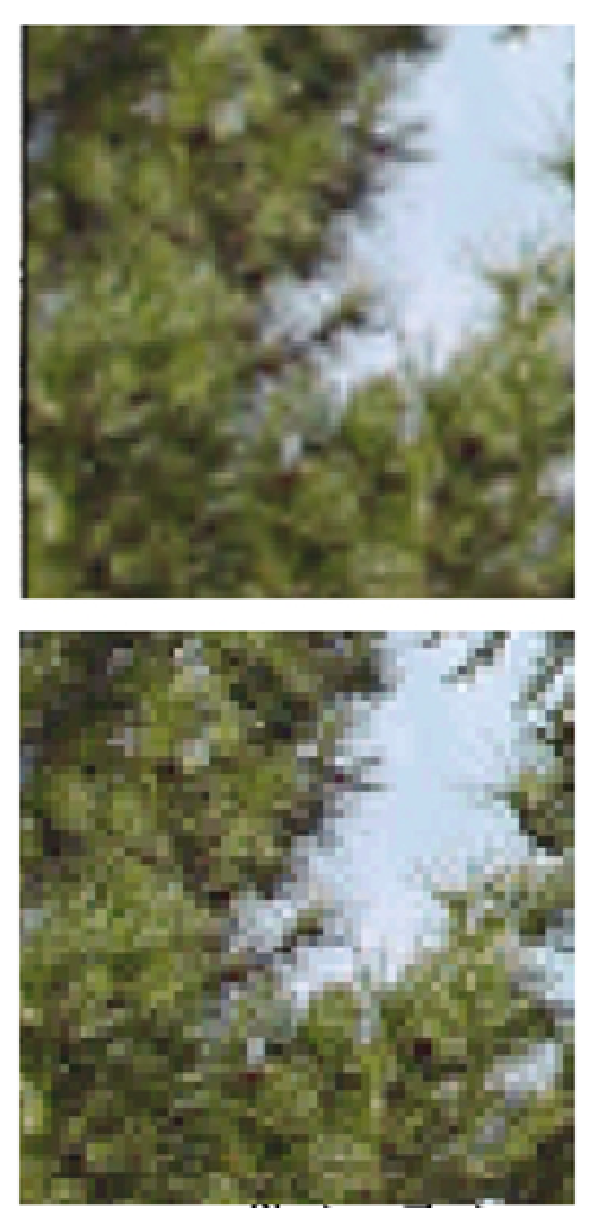
\includegraphics[angle=270,origin=b,width=0.75\textwidth]{expand4k.eps}
\caption{Expand4k}
\end{figure}

Ķ���������Ǥ��롥������ٲ����������֤��ƹ�����ٲ������������롥���٤ΥС�
���ȱ黻�ˤ��12��ʬ����ֽ�����Ԥ���RMGRP=12�ˡ����ϲ����ΰ�ư��Υ�������
�Ϥʤ����᥹�ƥ󥷥�׻��ǤϤʤ�mapdist=0�Ǥ��롥

\begin{screen}
\tiny
\begin{verbatim}
void expand4k(Uint *p, struct X *r)
#if !defined(EMAX5) && !defined(EMAX6)
  for (top=0; top<RRANGE; top+=RMGRP) { /* scan-lines */
    for (rofs=0; rofs<RMGRP; rofs++) { /* will be parallelized by multi-chip (M/#chip) */
      for (CHIP=0; CHIP<NCHIP; CHIP++) { /* will be parallelized by multi-chip (M/#chip) */
        int idx = CHIP*RRANGE+top+rofs;
        int k = idx*HT/768;
        int kfraq = (((idx*HT)<<4)/768)&15; /* 4bit */
        int kad = 16-ad(kfraq,8);
        int sk1 = ss(kfraq,8);
        int sk2 = ss(8,kfraq);
        Uint *pp = p+k*WD;
        Uint *rp = r->X[idx];
        for (cofs=0; cofs<1024; cofs++) { /* ������4095�ޤ� */
          int p1 = cofs*WD/1024;
          int lfraq = (((cofs*WD)<<4)/1024)&15; /* 4bit */
          int lad = 16-ad(lfraq,8);
          int sl1 = ss(lfraq,8);
          int sl2 = ss(8,lfraq);
          int r1 = kad*lad; /* 4bit*4bit */
          int r3 = kad*sl1; /* 4bit*4bit */
          int r2 = kad*sl2; /* 4bit*4bit */
          int r5 = sk1*lad; /* 4bit*4bit */
          int r9 = sk1*sl1; /* 4bit*4bit */
          int r8 = sk1*sl2; /* 4bit*4bit */
          int r4 = sk2*lad; /* 4bit*4bit */
          int r7 = sk2*sl1; /* 4bit*4bit */
          int r6 = sk2*sl2; /* 4bit*4bit */
          *rp = (unsigned int)((pp[p1]>>24&0xff)*r1
              +  (pp[p1   -1]>>24&0xff)*r2 + (pp[p1   +1]>>24&0xff)*r3 + (pp[p1-WD  ]>>24&0xff)*r4 + (pp[p1+WD  ]>>24&0xff)*r5
              +  (pp[p1-WD-1]>>24&0xff)*r6 + (pp[p1-WD+1]>>24&0xff)*r7 + (pp[p1+WD-1]>>24&0xff)*r8 + (pp[p1+WD+1]>>24&0xff)*r9)/256<<24
              | (unsigned int)((pp[p1]>>16&0xff)*r1
              +  (pp[p1   -1]>>16&0xff)*r2 + (pp[p1   +1]>>16&0xff)*r3 + (pp[p1-WD  ]>>16&0xff)*r4 + (pp[p1+WD  ]>>16&0xff)*r5
              +  (pp[p1-WD-1]>>16&0xff)*r6 + (pp[p1-WD+1]>>16&0xff)*r7 + (pp[p1+WD-1]>>16&0xff)*r8 + (pp[p1+WD+1]>>16&0xff)*r9)/256<<16
              | (unsigned int)((pp[p1]>> 8&0xff)*r1
              +  (pp[p1   -1]>> 8&0xff)*r2 + (pp[p1   +1]>> 8&0xff)*r3 + (pp[p1-WD  ]>> 8&0xff)*r4 + (pp[p1+WD  ]>> 8&0xff)*r5
              +  (pp[p1-WD-1]>> 8&0xff)*r6 + (pp[p1-WD+1]>> 8&0xff)*r7 + (pp[p1+WD-1]>> 8&0xff)*r8 + (pp[p1+WD+1]>> 8&0xff)*r9)/256<<8;
          rp++;
        }
      }
    }
  }
#endif
\end{verbatim}
\end{screen}

\begin{screen}
\tiny
\begin{verbatim}
  for (top=0; top<RRANGE; top+=RMGRP) { /* scan-lines */
    for (rofs=0; rofs<RMGRP; rofs++) { /* will be parallelized by multi-chip (M/#chip) */
      for (CHIP=0; CHIP<NCHIP; CHIP++) { /* will be parallelized by multi-chip (M/#chip) */
        int idx = CHIP*RRANGE+top+rofs;
        int k = idx*HT/768;
        int kfraq = (((idx*HT)<<4)/768)&15; /* 4bit */
        int kad = 16-ad(kfraq,8);
        int sk1 = ss(kfraq,8);
        int sk2 = ss(8,kfraq);
        Uint *pp = p+k*WD;
        Uint *rp = r->X[idx];
        for (cofs=0; cofs<1024; cofs++) { /* ������4095�ޤ� */
          int p1 = cofs*WD/1024;
          int lfraq = (((cofs*WD)<<4)/1024)&15; /* 4bit */
          int lad = 16-ad(lfraq,8);
          int sl1 = ss(lfraq,8);
          int sl2 = ss(8,lfraq);
          int r1 = kad*lad; /* 4bit*4bit */
          int r3 = kad*sl1; /* 4bit*4bit */
          int r2 = kad*sl2; /* 4bit*4bit */
          int r5 = sk1*lad; /* 4bit*4bit */
          int r9 = sk1*sl1; /* 4bit*4bit */
          int r8 = sk1*sl2; /* 4bit*4bit */
          int r4 = sk2*lad; /* 4bit*4bit */
          int r7 = sk2*sl1; /* 4bit*4bit */
          int r6 = sk2*sl2; /* 4bit*4bit */
          Uint ph, pl, x;
          ph = madd(mmul(b2h(pp[p1     ], 1), r1), mmul(b2h(pp[p1-1], 1), r2));
          ph = madd(mmul(b2h(pp[p1   +1], 1), r3), ph);
          ph = madd(mmul(b2h(pp[p1-WD  ], 1), r4), ph);
          ph = madd(mmul(b2h(pp[p1+WD  ], 1), r5), ph);
          ph = madd(mmul(b2h(pp[p1-WD-1], 1), r6), ph);
          ph = madd(mmul(b2h(pp[p1-WD+1], 1), r7), ph);
          ph = madd(mmul(b2h(pp[p1+WD-1], 1), r8), ph);
          ph = madd(mmul(b2h(pp[p1+WD+1], 1), r9), ph);
          pl = madd(mmul(b2h(pp[p1     ], 0), r1), mmul(b2h(pp[p1-1], 0), r2));
          pl = madd(mmul(b2h(pp[p1   +1], 0), r3), pl);
          pl = madd(mmul(b2h(pp[p1-WD  ], 0), r4), pl);
          pl = madd(mmul(b2h(pp[p1+WD  ], 0), r5), pl);
          pl = madd(mmul(b2h(pp[p1-WD-1], 0), r6), pl);
          pl = madd(mmul(b2h(pp[p1-WD+1], 0), r7), pl);
          pl = madd(mmul(b2h(pp[p1+WD-1], 0), r8), pl);
          pl = madd(mmul(b2h(pp[p1+WD+1], 0), r9), pl);
          *rp = h2b(msrl(ph, 8), 1) | h2b(msrl(pl, 8), 0);
          rp++;
        }
      }
    }
  }
\end{verbatim}
\end{screen}

\begin{screen}
\tiny
\begin{verbatim}
  Ull  LOOP1, LOOP0;
  Ull  INIT1, INIT0;
  Ull  AR[64][4];                     /* output of EX     in each unit */
  Ull  BR[64][4][4];                  /* output registers in each unit */
  Ull  r0, r1, r2, r3, r4, r5, r6, r7, r8, r9, r10, r11, r12, r13, r14, r15;
  Ull  r16, r17, r18, r19, r20, r21, r22, r23, r24, r25, r26, r27, r28, r29, r30, r31;
  Ull  cc0, cc1, cc2, cc3, ex0, ex1;
  for (top=0; top<RRANGE; top+=RMGRP) { /* will be parallelized by multi-chip (M/#chip) */
    for (rofs=0; rofs<RMGRP; rofs++) { /* will be parallelized by multi-chip (M/#chip) */
      Sll  kad[NCHIP], sk1[NCHIP], sk2[NCHIP];
      Uint *pp[NCHIP], *p0[NCHIP], *p1[NCHIP], *p2[NCHIP], *rp[NCHIP];
      for (CHIP=0; CHIP<NCHIP; CHIP++) { /* will be parallelized by multi-chip (M/#chip) */
        int  idx   = CHIP*RRANGE+top+rofs;
        int  k     = idx*HT/768;
        int  kfraq = (((idx*HT)<<4)/768)&15; /* 4bit */
        kad[CHIP]  = 16-ad(kfraq,8);
        sk1[CHIP]  = ss(kfraq,8);
        sk2[CHIP]  = ss(8,kfraq);
        pp[CHIP]   = p+k*WD;
        p0[CHIP]   = pp[CHIP]-WD;
        p1[CHIP]   = pp[CHIP];
        p2[CHIP]   = pp[CHIP]+WD;
        rp[CHIP]   = r->X[idx];
      }
//EMAX5A begin expand4k mapdist=0
 /*2*/for (CHIP=0; CHIP<NCHIP; CHIP++) { /* output channels are parallelized by multi-chip (OC/#chip) */
   /*1*/for (INIT0=1,LOOP0=1024,cofs=0-WD; LOOP0--; INIT0=0) {       /* stage#0 *//* mapped to FOR() on BR[63][0][0] */
 /*@0,1*/ exe(OP_ADD,       &cofs, cofs,      EXP_H3210, WD,    EXP_H3210, 0LL, EXP_H3210, OP_AND, 0x00000000ffffffffLL, OP_NOP, 0LL);
 /*@1,0*/ exe(OP_NOP,       &r0,   cofs,      EXP_H3210, 0LL,   EXP_H3210, 0LL, EXP_H3210, OP_AND, ~1023LL,  OP_SRL,  8LL);
 /*@1,1*/ exe(OP_NOP,       &r4,   cofs,      EXP_H3210, 0LL,   EXP_H3210, 0LL, EXP_H3210, OP_AND,  0x3c0LL, OP_SRL,  6LL);
 /*@2,0*/ exe(OP_ADD,       &r0,   pp[CHIP],  EXP_H3210, r0,    EXP_H3210, 0LL, EXP_H3210, OP_NOP,  0LL,     OP_NOP,  0LL);
 /*@2,1*/ exe(OP_MSUH,      &r1,   r4,        EXP_H3210, 8LL,   EXP_H3210, 0LL, EXP_H3210, OP_NOP,  0LL,     OP_NOP,  0LL);
 /*@2,2*/ exe(OP_MSUH,      &r2,   8LL,       EXP_H3210, r4,    EXP_H3210, 0LL, EXP_H3210, OP_NOP,  0LL,     OP_NOP,  0LL);
 /*@2,3*/ exe(OP_MSSAD,     &r3,   0LL,       EXP_H3210, r4,    EXP_H3210, 8LL, EXP_H3210, OP_NOP,  0LL,     OP_NOP,  0LL);
 /*@3,3*/ exe(OP_MSUH,      &r3,   16LL,      EXP_H3210, r3,    EXP_H3210, 0LL, EXP_H3210, OP_NOP,  0LL,     OP_NOP,  0LL);

 /*@4,1*/ exe(OP_MLUH,      &r21,  sk2[CHIP], EXP_H3210, r1,    EXP_H3210, 0LL, EXP_H3210, OP_NOP,  0LL,     OP_NOP,  0LL);
 /*@4,1*/ mop(OP_LDWR, 1,   &r10,  r0, -1276, MSK_D0,    (Ull)p0[CHIP],    WD,    0, 0, (Ull)NULL,       WD);
 /*@4,2*/ exe(OP_MLUH,      &r22,  sk2[CHIP], EXP_H3210, r2,    EXP_H3210, 0LL, EXP_H3210, OP_NOP,  0LL,     OP_NOP,  0LL);
 /*@4,2*/ mop(OP_LDWR, 1,   &r11,  r0, -1284, MSK_D0,    (Ull)p0[CHIP],    WD,    0, 0, (Ull)NULL,       WD);
 /*@4,3*/ exe(OP_MLUH,      &r23,  sk2[CHIP], EXP_H3210, r3,    EXP_H3210, 0LL, EXP_H3210, OP_NOP,  0LL,     OP_NOP,  0LL);
 /*@4,3*/ mop(OP_LDWR, 1,   &r12,  r0, -1280, MSK_D0,    (Ull)p0[CHIP],    WD,    0, 0, (Ull)NULL,       WD);

 /*@5,1*/ exe(OP_MLUH,      &r13,  r10,       EXP_B5410, r21,   EXP_H3210, 0LL, EXP_H3210, OP_NOP,  0LL,     OP_NOP,  0LL);
 /*@5,2*/ exe(OP_MLUH,      &r14,  r11,       EXP_B5410, r22,   EXP_H3210, 0LL, EXP_H3210, OP_NOP,  0LL,     OP_NOP,  0LL);
 /*@5,3*/ exe(OP_MLUH,      &r15,  r12,       EXP_B5410, r23,   EXP_H3210, 0LL, EXP_H3210, OP_NOP,  0LL,     OP_NOP,  0LL);

 /*@6,0*/ exe(OP_MAUH3,     &r16,  r13,       EXP_H3210, r14,   EXP_H3210, r15, EXP_H3210, OP_NOP,  0LL,     OP_NOP,  0LL);
 /*@6,1*/ exe(OP_MLUH,      &r13,  r10,       EXP_B7632, r21,   EXP_H3210, 0LL, EXP_H3210, OP_NOP,  0LL,     OP_NOP,  0LL);
 /*@6,2*/ exe(OP_MLUH,      &r14,  r11,       EXP_B7632, r22,   EXP_H3210, 0LL, EXP_H3210, OP_NOP,  0LL,     OP_NOP,  0LL);
 /*@6,3*/ exe(OP_MLUH,      &r15,  r12,       EXP_B7632, r23,   EXP_H3210, 0LL, EXP_H3210, OP_NOP,  0LL,     OP_NOP,  0LL);

 /*@7,0*/ exe(OP_MAUH3,     &r17,  r13,       EXP_H3210, r14,   EXP_H3210, r15, EXP_H3210, OP_NOP,  0LL,     OP_NOP,  0LL);
 /*@7,1*/ exe(OP_MLUH,      &r21,  kad[CHIP], EXP_H3210, r1,    EXP_H3210, 0LL, EXP_H3210, OP_NOP,  0LL,     OP_NOP,  0LL);
 /*@7,1*/ mop(OP_LDWR, 1,   &r10,  r0,     4, MSK_D0,    (Ull)p1[CHIP],    WD,    0, 0, (Ull)NULL,       WD);
 /*@7,2*/ exe(OP_MLUH,      &r22,  kad[CHIP], EXP_H3210, r2,    EXP_H3210, 0LL, EXP_H3210, OP_NOP,  0LL,     OP_NOP,  0LL);
 /*@7,2*/ mop(OP_LDWR, 1,   &r11,  r0,    -4, MSK_D0,    (Ull)p1[CHIP],    WD,    0, 0, (Ull)NULL,       WD);
 /*@7,3*/ exe(OP_MLUH,      &r23,  kad[CHIP], EXP_H3210, r3,    EXP_H3210, 0LL, EXP_H3210, OP_NOP,  0LL,     OP_NOP,  0LL);
 /*@7,3*/ mop(OP_LDWR, 1,   &r12,  r0,     0, MSK_D0,    (Ull)p1[CHIP],    WD,    0, 0, (Ull)NULL,       WD);

 /*@8,1*/ exe(OP_MLUH,      &r13,  r10,       EXP_B5410, r21,   EXP_H3210, 0LL, EXP_H3210, OP_NOP,  0LL,     OP_NOP,  0LL);
 /*@8,2*/ exe(OP_MLUH,      &r14,  r11,       EXP_B5410, r22,   EXP_H3210, 0LL, EXP_H3210, OP_NOP,  0LL,     OP_NOP,  0LL);
 /*@8,3*/ exe(OP_MLUH,      &r15,  r12,       EXP_B5410, r23,   EXP_H3210, 0LL, EXP_H3210, OP_NOP,  0LL,     OP_NOP,  0LL);

 /*@9,0*/ exe(OP_MAUH3,     &r18,  r13,       EXP_H3210, r14,   EXP_H3210, r15, EXP_H3210, OP_NOP,  0LL,     OP_NOP,  0LL);
 /*@9,1*/ exe(OP_MLUH,      &r13,  r10,       EXP_B7632, r21,   EXP_H3210, 0LL, EXP_H3210, OP_NOP,  0LL,     OP_NOP,  0LL);
 /*@9,2*/ exe(OP_MLUH,      &r14,  r11,       EXP_B7632, r22,   EXP_H3210, 0LL, EXP_H3210, OP_NOP,  0LL,     OP_NOP,  0LL);
 /*@9,3*/ exe(OP_MLUH,      &r15,  r12,       EXP_B7632, r23,   EXP_H3210, 0LL, EXP_H3210, OP_NOP,  0LL,     OP_NOP,  0LL);

 /*@10,0*/exe(OP_MAUH3,     &r19,  r13,       EXP_H3210, r14,   EXP_H3210, r15, EXP_H3210, OP_NOP,  0LL,     OP_NOP,  0LL);
 /*@10,1*/exe(OP_MLUH,      &r21,  sk1[CHIP], EXP_H3210, r1,    EXP_H3210, 0LL, EXP_H3210, OP_NOP,  0LL,     OP_NOP,  0LL);
 /*@10,1*/mop(OP_LDWR, 1,   &r10,  r0,  1284, MSK_D0,    (Ull)p2[CHIP],    WD,    0, 0, (Ull)NULL,       WD);
 /*@10,2*/exe(OP_MLUH,      &r22,  sk1[CHIP], EXP_H3210, r2,    EXP_H3210, 0LL, EXP_H3210, OP_NOP,  0LL,     OP_NOP,  0LL);
 /*@10,2*/mop(OP_LDWR, 1,   &r11,  r0,  1276, MSK_D0,    (Ull)p2[CHIP],    WD,    0, 0, (Ull)NULL,       WD);
 /*@10,3*/exe(OP_MLUH,      &r23,  sk1[CHIP], EXP_H3210, r3,    EXP_H3210, 0LL, EXP_H3210, OP_NOP,  0LL,     OP_NOP,  0LL);
 /*@10,3*/mop(OP_LDWR, 1,   &r12,  r0,  1280, MSK_D0,    (Ull)p2[CHIP],    WD,    0, 0, (Ull)NULL,       WD);

 /*@11,1*/exe(OP_MLUH,      &r13,  r10,       EXP_B5410, r21,   EXP_H3210, 0LL, EXP_H3210, OP_NOP,  0LL,     OP_NOP,  0LL);
 /*@11,2*/exe(OP_MLUH,      &r14,  r11,       EXP_B5410, r22,   EXP_H3210, 0LL, EXP_H3210, OP_NOP,  0LL,     OP_NOP,  0LL);
 /*@11,3*/exe(OP_MLUH,      &r15,  r12,       EXP_B5410, r23,   EXP_H3210, 0LL, EXP_H3210, OP_NOP,  0LL,     OP_NOP,  0LL);

 /*@12,0*/exe(OP_MAUH3,     &r20,  r13,       EXP_H3210, r14,   EXP_H3210, r15, EXP_H3210, OP_NOP,  0LL,     OP_NOP,  0LL);
 /*@12,1*/exe(OP_MLUH,      &r13,  r10,       EXP_B7632, r21,   EXP_H3210, 0LL, EXP_H3210, OP_NOP,  0LL,     OP_NOP,  0LL);
 /*@12,2*/exe(OP_MLUH,      &r14,  r11,       EXP_B7632, r22,   EXP_H3210, 0LL, EXP_H3210, OP_NOP,  0LL,     OP_NOP,  0LL);
 /*@12,3*/exe(OP_MLUH,      &r15,  r12,       EXP_B7632, r23,   EXP_H3210, 0LL, EXP_H3210, OP_NOP,  0LL,     OP_NOP,  0LL);

 /*@13,0*/exe(OP_MAUH3,     &r21,  r13,       EXP_H3210, r14,   EXP_H3210, r15, EXP_H3210, OP_NOP,  0LL,     OP_NOP,  0LL);

 /*@14,0*/exe(OP_MAUH3,     &r21,  r17,       EXP_H3210, r19,   EXP_H3210, r21, EXP_H3210, OP_OR,   0LL,     OP_SRLM, 8LL);
 /*@14,1*/exe(OP_MAUH3,     &r20,  r16,       EXP_H3210, r18,   EXP_H3210, r20, EXP_H3210, OP_OR,   0LL,     OP_SRLM, 8LL);

 /*@15,0*/exe(OP_MH2BW,     &r31,  r21,       EXP_H3210, r20,   EXP_H3210, 0LL, EXP_H3210, OP_NOP,  0LL,     OP_NOP,  0LL);
 /*@15,0*/mop(OP_STWR, 3,   &r31,  (Ull)(rp[CHIP]++),    0LL,   MSK_D0, (Ull)rp[CHIP],  1024, 0, 0, (Ull)NULL, 1024);
        }
      }
//EMAX5A end
    }
  }
//EMAX5A drain_dirty_lmm
\end{verbatim}
\end{screen}

\begin{figure}[htbp]
\center
\epsfile{file=filter+rmm-expand4k-emax6.eps,width=1.00\textwidth}
\caption{Expand4k}
\end{figure}

\clearpage

\subsection{Unsharp with stencil}

\begin{figure}[htbp]
\center
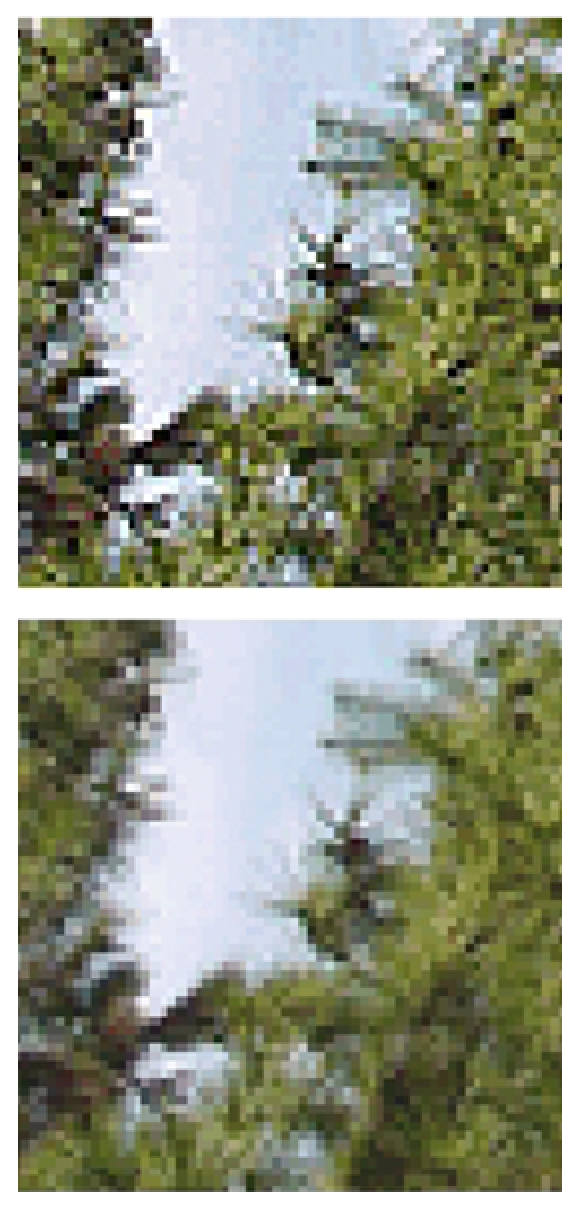
\includegraphics[angle=270,origin=b,width=0.75\textwidth]{unsharp.eps}
\caption{Unsharp}
\end{figure}

���å���Ĵ����3x3�����Բ��ե��륿�Ǥ��롥���٤ΥС����ȱ黻�ˤ�ꡤ6�ս�
��OMAP=6�ˤγơ��ˤĤ��ơ�10��ʬ�Υե��륿������Ԥ���RMGRP=10�ˡ����ƥ󥷥�
�׻��Ǥ���mapdist=1�Ǥ��롥

\begin{screen}
\tiny
\begin{verbatim}
void unsharp(Uchar *p, Uchar *r)
#if !defined(EMAX5) && !defined(EMAX6)
  for (top=PAD; top<HT-PAD; top++) { /* scan-lines */
    Uchar *p0 = p+((top  )*WD+(0  ))*4;  // p1 p5 p2
    Uchar *p1 = p+((top-1)*WD+(0-1))*4;  // p6 p0 p7
    Uchar *p2 = p+((top-1)*WD+(0+1))*4;  // p3 p8 p4
    Uchar *p3 = p+((top+1)*WD+(0-1))*4;
    Uchar *p4 = p+((top+1)*WD+(0+1))*4;
    Uchar *p5 = p+((top-1)*WD+(0  ))*4;
    Uchar *p6 = p+((top  )*WD+(0-1))*4;
    Uchar *p7 = p+((top  )*WD+(0+1))*4;
    Uchar *p8 = p+((top+1)*WD+(0  ))*4;
    Uchar *rp = r+((top  )*WD+(0  ))*4;
    for (cofs=0; cofs<WD; cofs++) {
      int t0,t1,t2;
      rp[0] = 0;
      t0 = p0[1]; t1 = p1[1]+p2[1]+p3[1]+p4[1]; t2 = p5[1]+p6[1]+p7[1]+p8[1];
      rp[1] = limitRGB(( t0 * 239 - t1 * 13 - t2 * 15 - t2/4) >> 7);
      t0 = p0[2]; t1 = p1[2]+p2[2]+p3[2]+p4[2]; t2 = p5[2]+p6[2]+p7[2]+p8[2];
      rp[2] = limitRGB(( t0 * 239 - t1 * 13 - t2 * 15 - t2/4) >> 7);
      t0 = p0[3]; t1 = p1[3]+p2[3]+p3[3]+p4[3]; t2 = p5[3]+p6[3]+p7[3]+p8[3];
      rp[3] = limitRGB(( t0 * 239 - t1 * 13 - t2 * 15 - t2/4) >> 7);
      p0+=4; p1+=4; p2+=4; p3+=4; p4+=4; p5+=4; p6+=4; p7+=4; p8+=4; rp+=4;
    }
  }
#endif
\end{verbatim}
\end{screen}

\begin{screen}
\tiny
\begin{verbatim}
  for (top=0; top<RRANGE; top+=RMGRP) { /* scan-lines */
    for (rofs=0; rofs<RMGRP; rofs++) { /* will be parallelized by multi-chip (M/#chip) */
      for (CHIP=0; CHIP<NCHIP; CHIP++) { /* will be parallelized by multi-chip (M/#chip) */
        int idx = (CHIP*RRANGE*OMAP+top+rofs)*WD;
        Uchar *p0 = p+(idx   +(0  ))*4;  // p1 p5 p2
        Uchar *p1 = p+(idx-WD+(0-1))*4;  // p6 p0 p7
        Uchar *p2 = p+(idx-WD+(0+1))*4;  // p3 p8 p4
        Uchar *p3 = p+(idx+WD+(0-1))*4;
        Uchar *p4 = p+(idx+WD+(0+1))*4;
        Uchar *p5 = p+(idx-WD+(0  ))*4;
        Uchar *p6 = p+(idx   +(0-1))*4;
        Uchar *p7 = p+(idx   +(0+1))*4;
        Uchar *p8 = p+(idx+WD+(0  ))*4;
        Uchar *rp = r+(idx   +(0  ))*4;
        for (cofs=0; cofs<WD; cofs++) {
          for (oc=0; oc<OMAP; oc++) {
            Uint pix0 = (oc*RRANGE*WD+cofs)*4+0;
            Uint pix1 = (oc*RRANGE*WD+cofs)*4+1;
            Uint pix2 = (oc*RRANGE*WD+cofs)*4+2;
            Uint pix3 = (oc*RRANGE*WD+cofs)*4+3;
            int t0,t1,t2;
            rp[pix0] = 0;
            t0 = p0[pix1]; t1 = p1[pix1]+p2[pix1]+p3[pix1]+p4[pix1]; t2 = p5[pix1]+p6[pix1]+p7[pix1]+p8[pix1];
            rp[pix1] = limitRGB(( t0 * 239 - t1 * 13 - t2 * 15 - t2/4) >> 7);
            t0 = p0[pix2]; t1 = p1[pix2]+p2[pix2]+p3[pix2]+p4[pix2]; t2 = p5[pix2]+p6[pix2]+p7[pix2]+p8[pix2];
            rp[pix2] = limitRGB(( t0 * 239 - t1 * 13 - t2 * 15 - t2/4) >> 7);
            t0 = p0[pix3]; t1 = p1[pix3]+p2[pix3]+p3[pix3]+p4[pix3]; t2 = p5[pix3]+p6[pix3]+p7[pix3]+p8[pix3];
            rp[pix3] = limitRGB(( t0 * 239 - t1 * 13 - t2 * 15 - t2/4) >> 7);
          }
        }
      }
    }
  }
\end{verbatim}
\end{screen}

\begin{screen}
\tiny
\begin{verbatim}
  Ull  LOOP1, LOOP0;
  Ull  INIT1, INIT0;
  Ull  AR[64][4];                     /* output of EX     in each unit */
  Ull  BR[64][4][4];                  /* output registers in each unit */
  Ull  r0, r1, r2, r3, r4, r5, r6, r7, r8, r9, r10, r11, r12, r13, r14, r15;
  Ull  r16, r17, r18, r19, r20, r21, r22, r23, r24, r25, r26, r27, r28, r29, r30, r31;
  Ull  cc0, cc1, cc2, cc3, ex0, ex1;
  for (top=0; top<RRANGE; top+=RMGRP) { /* scan-lines */
    for (rofs=0; rofs<RMGRP; rofs++) { /* will be parallelized by multi-chip (M/#chip) */
      Uchar *pp0[NCHIP], *pc0[NCHIP], *pn0[NCHIP], *rc0[NCHIP];
      Uchar *pp1[NCHIP], *pc1[NCHIP], *pn1[NCHIP], *rc1[NCHIP];
      Uchar *pp2[NCHIP], *pc2[NCHIP], *pn2[NCHIP], *rc2[NCHIP];
      Uchar *pp3[NCHIP], *pc3[NCHIP], *pn3[NCHIP], *rc3[NCHIP];
      Uchar *pp4[NCHIP], *pc4[NCHIP], *pn4[NCHIP], *rc4[NCHIP];
      Uchar *pp5[NCHIP], *pc5[NCHIP], *pn5[NCHIP], *rc5[NCHIP];
      for (CHIP=0; CHIP<NCHIP; CHIP++) { /* will be parallelized by multi-chip (M/#chip) */
        int idx = (CHIP*RRANGE*OMAP+top+rofs)*WD*4;
        pp0[CHIP] = p+idx+RRANGE*WD* 0-1280;  pc0[CHIP] = p+idx+RRANGE*WD* 0; pn0[CHIP] = p+idx+RRANGE*WD* 0+1280; rc0[CHIP] = r+idx+RRANGE*WD* 0;
        pp1[CHIP] = p+idx+RRANGE*WD* 4-1280;  pc1[CHIP] = p+idx+RRANGE*WD* 4; pn1[CHIP] = p+idx+RRANGE*WD* 4+1280; rc1[CHIP] = r+idx+RRANGE*WD* 4;
        pp2[CHIP] = p+idx+RRANGE*WD* 8-1280;  pc2[CHIP] = p+idx+RRANGE*WD* 8; pn2[CHIP] = p+idx+RRANGE*WD* 8+1280; rc2[CHIP] = r+idx+RRANGE*WD* 8;
        pp3[CHIP] = p+idx+RRANGE*WD*12-1280;  pc3[CHIP] = p+idx+RRANGE*WD*12; pn3[CHIP] = p+idx+RRANGE*WD*12+1280; rc3[CHIP] = r+idx+RRANGE*WD*12;
        pp4[CHIP] = p+idx+RRANGE*WD*16-1280;  pc4[CHIP] = p+idx+RRANGE*WD*16; pn4[CHIP] = p+idx+RRANGE*WD*16+1280; rc4[CHIP] = r+idx+RRANGE*WD*16;
        pp5[CHIP] = p+idx+RRANGE*WD*20-1280;  pc5[CHIP] = p+idx+RRANGE*WD*20; pn5[CHIP] = p+idx+RRANGE*WD*20+1280; rc5[CHIP] = r+idx+RRANGE*WD*20;
      }
//EMAX5A begin unsharp mapdist=1
 /*2*/for (CHIP=0; CHIP<NCHIP; CHIP++) { /* output channels are parallelized by multi-chip (OC/#chip) */
   /*1*/for (INIT0=1,LOOP0=WD,cofs=0-4; LOOP0--; INIT0=0) {       /* stage#0 *//* mapped to FOR() on BR[63][0][0] */
 /*@0,1*/ exe(OP_ADD,       &cofs, cofs,      EXP_H3210, 4LL,  EXP_H3210, 0LL, EXP_H3210, OP_AND, 0x00000000ffffffffLL, OP_NOP, 0LL);
          /*map0*/
 /*@1,0*/ exe(OP_ADD,       &pofs, pc0[CHIP], EXP_H3210, cofs, EXP_H3210, 0LL, EXP_H3210, OP_NOP,  0LL,    OP_NOP,  0LL);
 /*@2,0*/ mop(OP_LDWR, 1,   &r1,   pofs,     -1276, MSK_D0,    (Ull)pp0[CHIP], WD,    0, 0, (Ull)NULL,   WD);
 /*@2,0*/ mop(OP_LDWR, 1,   &r2,   pofs,     -1284, MSK_D0,    (Ull)pp0[CHIP], WD,    0, 0, (Ull)NULL,   WD);
 /*@2,1*/ mop(OP_LDWR, 1,   &r5,   pofs,     -1280, MSK_D0,    (Ull)pp0[CHIP], WD,    0, 0, (Ull)NULL,   WD);
 /*@3,0*/ exe(OP_MAUH,      &r11,  r1,        EXP_B5410, r2,   EXP_B5410, 0LL, EXP_H3210, OP_NOP,  0LL,    OP_NOP,  0LL);
 /*@3,0*/ mop(OP_LDWR, 1,   &r6,   pofs,      4,    MSK_D0,    (Ull)pc0[CHIP], WD,    0, 0, (Ull)NULL,   WD);
 /*@3,0*/ mop(OP_LDWR, 1,   &r7,   pofs,     -4,    MSK_D0,    (Ull)pc0[CHIP], WD,    0, 0, (Ull)NULL,   WD);
 /*@3,1*/ exe(OP_MAUH,      &r12,  r1,        EXP_B7632, r2,   EXP_B7632, 0LL, EXP_H3210, OP_NOP,  0LL,    OP_NOP,  0LL);
 /*@3,1*/ mop(OP_LDWR, 1,   &r0,   pofs,      0,    MSK_D0,    (Ull)pc0[CHIP], WD,    0, 0, (Ull)NULL,   WD);
 /*@4,0*/ exe(OP_MLUH,      &r20,  r0,        EXP_B5410, 239,  EXP_H3210, 0LL, EXP_H3210, OP_NOP,  0LL,    OP_NOP,  0LL);
 /*@4,0*/ mop(OP_LDWR, 1,   &r3,   pofs,      1284, MSK_D0,    (Ull)pn0[CHIP], WD,    0, 0, (Ull)NULL,   WD);
 /*@4,0*/ mop(OP_LDWR, 1,   &r4,   pofs,      1276, MSK_D0,    (Ull)pn0[CHIP], WD,    0, 0, (Ull)NULL,   WD);
 /*@4,1*/ exe(OP_MLUH,      &r21,  r0,        EXP_B7632, 239,  EXP_H3210, 0LL, EXP_H3210, OP_NOP,  0LL,    OP_NOP,  0LL);
 /*@4,1*/ mop(OP_LDWR, 1,   &r8,   pofs,      1280, MSK_D0,    (Ull)pn0[CHIP], WD,    0, 0, (Ull)NULL,   WD);
 /*@4,2*/ exe(OP_MAUH,      &r15,  r5,        EXP_B5410, r6,   EXP_B5410, 0LL, EXP_H3210, OP_NOP,  0LL,    OP_NOP,  0LL);
 /*@4,3*/ exe(OP_MAUH,      &r16,  r5,        EXP_B7632, r6,   EXP_B7632, 0LL, EXP_H3210, OP_NOP,  0LL,    OP_NOP,  0LL);
 /*@5,0*/ exe(OP_MAUH3,     &r11,  r3,        EXP_B5410, r4,   EXP_B5410, r11, EXP_H3210, OP_NOP,  0LL,    OP_NOP,  0LL);
 /*@5,1*/ exe(OP_MAUH3,     &r12,  r3,        EXP_B7632, r4,   EXP_B7632, r12, EXP_H3210, OP_NOP,  0LL,    OP_NOP,  0LL);
 /*@6,0*/ exe(OP_MLUH,      &r13,  r11,       EXP_H3210, 13,   EXP_H3210, 0LL, EXP_H3210, OP_NOP,  0LL,    OP_NOP,  0LL);
 /*@6,1*/ exe(OP_MLUH,      &r14,  r12,       EXP_H3210, 13,   EXP_H3210, 0LL, EXP_H3210, OP_NOP,  0LL,    OP_NOP,  0LL);
 /*@6,2*/ exe(OP_MAUH3,     &r15,  r7,        EXP_B5410, r8,   EXP_B5410, r15, EXP_H3210, OP_NOP,  0LL,    OP_NOP,  0LL);
 /*@6,3*/ exe(OP_MAUH3,     &r16,  r7,        EXP_B7632, r8,   EXP_B7632, r16, EXP_H3210, OP_NOP,  0LL,    OP_NOP,  0LL);
 /*@7,0*/ exe(OP_NOP,       &r7,   r15,       EXP_H3210, 0LL,  EXP_H3210, 0LL, EXP_H3210, OP_OR,   0LL,    OP_SRLM, 2LL);
 /*@7,1*/ exe(OP_MLUH,      &r17,  r15,       EXP_H3210, 15,   EXP_H3210, 0LL, EXP_H3210, OP_NOP,  0LL,    OP_NOP,  0LL);
 /*@7,2*/ exe(OP_NOP,       &r8,   r16,       EXP_H3210, 0LL,  EXP_H3210, 0LL, EXP_H3210, OP_OR,   0LL,    OP_SRLM, 2LL);
 /*@7,3*/ exe(OP_MLUH,      &r18,  r16,       EXP_H3210, 15,   EXP_H3210, 0LL, EXP_H3210, OP_NOP,  0LL,    OP_NOP,  0LL);
 /*@8,0*/ exe(OP_MSUH3,     &r10,  r20,       EXP_H3210, r7,   EXP_H3210, r17, EXP_H3210, OP_NOP,  0LL,    OP_NOP,  0LL);
 /*@8,1*/ exe(OP_MSUH3,     &r11,  r21,       EXP_H3210, r8,   EXP_H3210, r18, EXP_H3210, OP_NOP,  0LL,    OP_NOP,  0LL);
 /*@9,0*/ exe(OP_MSUH,      &r20,  r10,       EXP_H3210, r13,  EXP_H3210, 0LL, EXP_H3210, OP_OR,   0LL,    OP_SRLM, 7LL);
 /*@9,1*/ exe(OP_MSUH,      &r21,  r11,       EXP_H3210, r14,  EXP_H3210, 0LL, EXP_H3210, OP_OR,   0LL,    OP_SRLM, 7LL);
 /*@10,0*/exe(OP_MH2BW,     &r31,  r21,       EXP_H3210, r20,  EXP_H3210, 0LL, EXP_H3210, OP_NOP,  0LL,    OP_NOP,  0LL);
 /*@10,0*/mop(OP_STWR, 3,   &r31,  rc0[CHIP], cofs, MSK_D0,    rc0[CHIP],      WD,    0, 0, (Ull)NULL,   WD);
       :
          /*map5*/
 /*@46,1*/exe(OP_ADD,       &pofs, pc5[CHIP], EXP_H3210, cofs, EXP_H3210, 0LL, EXP_H3210, OP_NOP,  0LL,    OP_NOP,  0LL);
 /*@47,0*/mop(OP_LDWR, 1,   &r1,   pofs,     -1276, MSK_D0,    (Ull)pp5[CHIP], WD,    0, 0, (Ull)NULL,   WD);
 /*@47,0*/mop(OP_LDWR, 1,   &r2,   pofs,     -1284, MSK_D0,    (Ull)pp5[CHIP], WD,    0, 0, (Ull)NULL,   WD);
 /*@47,1*/mop(OP_LDWR, 1,   &r5,   pofs,     -1280, MSK_D0,    (Ull)pp5[CHIP], WD,    0, 0, (Ull)NULL,   WD);
 /*@48,0*/exe(OP_MAUH,      &r11,  r1,        EXP_B5410, r2,   EXP_B5410, 0LL, EXP_H3210, OP_NOP,  0LL,    OP_NOP,  0LL);
 /*@48,0*/mop(OP_LDWR, 1,   &r6,   pofs,      4,    MSK_D0,    (Ull)pc5[CHIP], WD,    0, 0, (Ull)NULL,   WD);
 /*@48,0*/mop(OP_LDWR, 1,   &r7,   pofs,     -4,    MSK_D0,    (Ull)pc5[CHIP], WD,    0, 0, (Ull)NULL,   WD);
 /*@48,1*/exe(OP_MAUH,      &r12,  r1,        EXP_B7632, r2,   EXP_B7632, 0LL, EXP_H3210, OP_NOP,  0LL,    OP_NOP,  0LL);
 /*@48,1*/mop(OP_LDWR, 1,   &r0,   pofs,      0,    MSK_D0,    (Ull)pc5[CHIP], WD,    0, 0, (Ull)NULL,   WD);
 /*@49,0*/exe(OP_MLUH,      &r20,  r0,        EXP_B5410, 239,  EXP_H3210, 0LL, EXP_H3210, OP_NOP,  0LL,    OP_NOP,  0LL);
 /*@49,0*/mop(OP_LDWR, 1,   &r3,   pofs,      1284, MSK_D0,    (Ull)pn5[CHIP], WD,    0, 0, (Ull)NULL,   WD);
 /*@49,0*/mop(OP_LDWR, 1,   &r4,   pofs,      1276, MSK_D0,    (Ull)pn5[CHIP], WD,    0, 0, (Ull)NULL,   WD);
 /*@49,1*/exe(OP_MLUH,      &r21,  r0,        EXP_B7632, 239,  EXP_H3210, 0LL, EXP_H3210, OP_NOP,  0LL,    OP_NOP,  0LL);
 /*@49,1*/mop(OP_LDWR, 1,   &r8,   pofs,      1280, MSK_D0,    (Ull)pn5[CHIP], WD,    0, 0, (Ull)NULL,   WD);
 /*@49,2*/exe(OP_MAUH,      &r15,  r5,        EXP_B5410, r6,   EXP_B5410, 0LL, EXP_H3210, OP_NOP,  0LL,    OP_NOP,  0LL);
 /*@49,3*/exe(OP_MAUH,      &r16,  r5,        EXP_B7632, r6,   EXP_B7632, 0LL, EXP_H3210, OP_NOP,  0LL,    OP_NOP,  0LL);
 /*@50,0*/exe(OP_MAUH3,     &r11,  r3,        EXP_B5410, r4,   EXP_B5410, r11, EXP_H3210, OP_NOP,  0LL,    OP_NOP,  0LL);
 /*@50,1*/exe(OP_MAUH3,     &r12,  r3,        EXP_B7632, r4,   EXP_B7632, r12, EXP_H3210, OP_NOP,  0LL,    OP_NOP,  0LL);
 /*@51,0*/exe(OP_MLUH,      &r13,  r11,       EXP_H3210, 13,   EXP_H3210, 0LL, EXP_H3210, OP_NOP,  0LL,    OP_NOP,  0LL);
 /*@51,1*/exe(OP_MLUH,      &r14,  r12,       EXP_H3210, 13,   EXP_H3210, 0LL, EXP_H3210, OP_NOP,  0LL,    OP_NOP,  0LL);
 /*@51,2*/exe(OP_MAUH3,     &r15,  r7,        EXP_B5410, r8,   EXP_B5410, r15, EXP_H3210, OP_NOP,  0LL,    OP_NOP,  0LL);
 /*@51,3*/exe(OP_MAUH3,     &r16,  r7,        EXP_B7632, r8,   EXP_B7632, r16, EXP_H3210, OP_NOP,  0LL,    OP_NOP,  0LL);
 /*@52,0*/exe(OP_NOP,       &r7,   r15,       EXP_H3210, 0LL,  EXP_H3210, 0LL, EXP_H3210, OP_OR,   0LL,    OP_SRLM, 2LL);
 /*@52,1*/exe(OP_MLUH,      &r17,  r15,       EXP_H3210, 15,   EXP_H3210, 0LL, EXP_H3210, OP_NOP,  0LL,    OP_NOP,  0LL);
 /*@52,2*/exe(OP_NOP,       &r8,   r16,       EXP_H3210, 0LL,  EXP_H3210, 0LL, EXP_H3210, OP_OR,   0LL,    OP_SRLM, 2LL);
 /*@52,3*/exe(OP_MLUH,      &r18,  r16,       EXP_H3210, 15,   EXP_H3210, 0LL, EXP_H3210, OP_NOP,  0LL,    OP_NOP,  0LL);
 /*@53,0*/exe(OP_MSUH3,     &r10,  r20,       EXP_H3210, r7,   EXP_H3210, r17, EXP_H3210, OP_NOP,  0LL,    OP_NOP,  0LL);
 /*@53,1*/exe(OP_MSUH3,     &r11,  r21,       EXP_H3210, r8,   EXP_H3210, r18, EXP_H3210, OP_NOP,  0LL,    OP_NOP,  0LL);
 /*@54,0*/exe(OP_MSUH,      &r20,  r10,       EXP_H3210, r13,  EXP_H3210, 0LL, EXP_H3210, OP_OR,   0LL,    OP_SRLM, 7LL);
 /*@54,1*/exe(OP_MSUH,      &r21,  r11,       EXP_H3210, r14,  EXP_H3210, 0LL, EXP_H3210, OP_OR,   0LL,    OP_SRLM, 7LL);
 /*@55,0*/exe(OP_MH2BW,     &r31,  r21,       EXP_H3210, r20,  EXP_H3210, 0LL, EXP_H3210, OP_NOP,  0LL,    OP_NOP,  0LL);
 /*@55,0*/mop(OP_STWR, 3,   &r31,  rc5[CHIP], cofs, MSK_D0,    rc5[CHIP],      WD,    0, 0, (Ull)NULL,   WD);
        }
      }
//EMAX5A end
    }
  }
//EMAX5A drain_dirty_lmm
\end{verbatim}
\end{screen}

\begin{figure}[htbp]
\center
\epsfile{file=filter+rmm-unsharp-emax6.eps,width=1.00\textwidth}
\caption{Unsharp}
\end{figure}

\clearpage

\subsection{Blur with stencil}

\begin{figure}[htbp]
\center
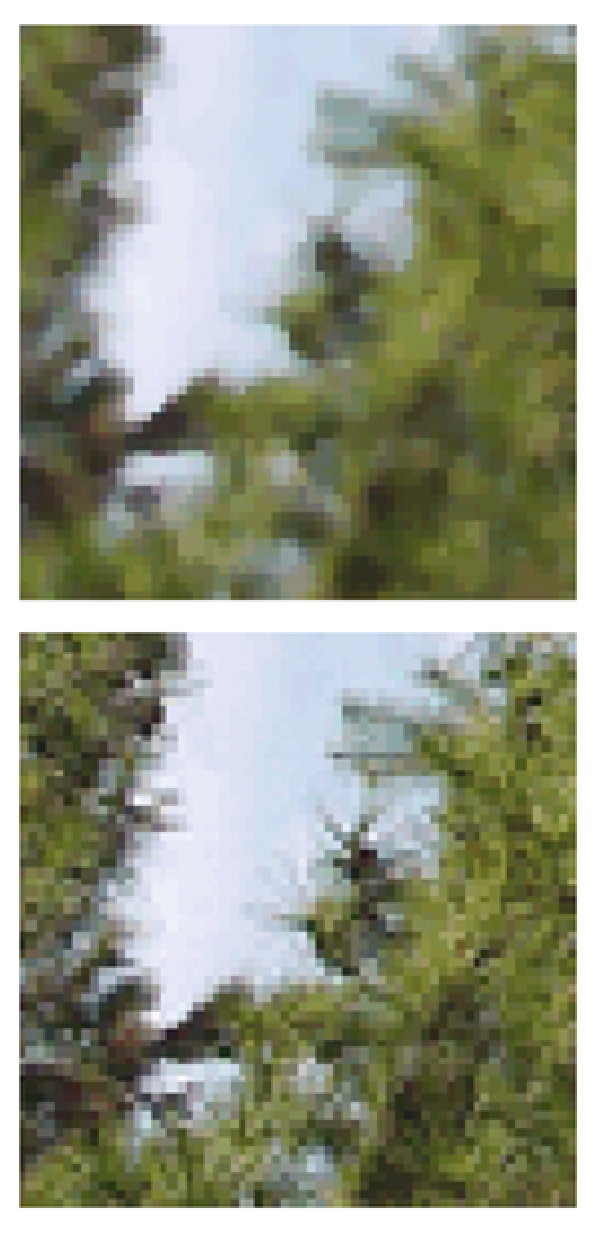
\includegraphics[angle=270,origin=b,width=0.55\textwidth]{blur.eps}
\caption{Blur}
\end{figure}

3x3�Υѥ��ץ饤�󲽥�ǥ�����ե��륿�Ǥ��롥���٤ΥС����ȱ黻�ˤ�ꡤ4�ս�
��OMAP=4�ˤγơ��ˤĤ��ơ�15��ʬ�Υե��륿������Ԥ���RMGRP=15�ˡ����ƥ󥷥�
�׻��Ǥ���mapdist=1�Ǥ��롥

\begin{screen}
\tiny
\begin{verbatim}
void blur(Uint *p, Uint *r)
#if !defined(EMAX5) && !defined(EMAX6)
  for (top=PAD; top<HT-PAD; top++) { /* scan-lines */
    Uint *p0 = p+(top  )*WD  ;
    Uint *p1 = p+(top  )*WD  ;
    Uint *p2 = p+(top  )*WD-1;
    Uint *p3 = p+(top  )*WD+1;
    Uint *p4 = p+(top-1)*WD  ;
    Uint *p5 = p+(top+1)*WD  ;
    Uint *p6 = p+(top-1)*WD-1;
    Uint *p7 = p+(top-1)*WD+1;
    Uint *p8 = p+(top+1)*WD-1;
    Uint *p9 = p+(top+1)*WD+1;
    Uint *rp = r+(top  )*WD  ;
    for (cofs=0; cofs<WD; cofs++) {
      *rp = (Uint)((*p1>>24&0xff)*20
          +  (*p2>>24&0xff)*12 + (*p3>>24&0xff)*12 + (*p4>>24&0xff)*12 + (*p5>>24&0xff)*12
          +  (*p6>>24&0xff)* 8 + (*p7>>24&0xff)* 8 + (*p8>>24&0xff)* 8 + (*p9>>24&0xff)* 8)/100<<24
          | (Uint)((*p1>>16&0xff)*20
          +  (*p2>>16&0xff)*12 + (*p3>>16&0xff)*12 + (*p4>>16&0xff)*12 + (*p5>>16&0xff)*12
          +  (*p6>>16&0xff)* 8 + (*p7>>16&0xff)* 8 + (*p8>>16&0xff)* 8 + (*p9>>16&0xff)* 8)/100<<16
          | (Uint)((*p1>> 8&0xff)*20
          +  (*p2>> 8&0xff)*12 + (*p3>> 8&0xff)*12 + (*p4>> 8&0xff)*12 + (*p5>> 8&0xff)*12
          +  (*p6>> 8&0xff)* 8 + (*p7>> 8&0xff)* 8 + (*p8>> 8&0xff)* 8 + (*p9>> 8&0xff)* 8)/100<<8;
      p0++; p1++; p2++; p3++; p4++; p5++; p6++; p7++; p8++; p9++; rp++;
    }
  }
#endif
\end{verbatim}
\end{screen}

\begin{screen}
\tiny
\begin{verbatim}
  for (top=PAD; top<HT-PAD; top++) { /* scan-lines */
    Uint *p0 = p+(top  )*WD  ;
    Uint *p1 = p+(top  )*WD  ;
    Uint *p2 = p+(top  )*WD-1;
    Uint *p3 = p+(top  )*WD+1;
    Uint *p4 = p+(top-1)*WD  ;
    Uint *p5 = p+(top+1)*WD  ;
    Uint *p6 = p+(top-1)*WD-1;
    Uint *p7 = p+(top-1)*WD+1;
    Uint *p8 = p+(top+1)*WD-1;
    Uint *p9 = p+(top+1)*WD+1;
    Uint *rp = r+(top  )*WD  ;
    for (cofs=0; cofs<WD; cofs++) {
      Uint s0,s1,s2,s3,s4,s5,s6,s7,s8;
      Uint t0,t1,t2;
      s0=*p1;s1=*p2;s2=*p3;s3=*p4;s4=*p5;s5=*p6;s6=*p7;s7=*p8;s8=*p9;
      /*��������������  ��������������  ��������������  ��������������  ��������������  ��������������  ������
        ��������������  �����㣳�����  ��������������  �����㣳�����  ������  ������  ������  �����  ������
        ���˨��˨��˨�  ��������������  ���˨��˨��˨�  ��������������  ���˨������˨�  ��������������  ���˨�
        ��������������  �����㣰�㣲��  ���ݨ������ݨ�  ��    ��    ��  ��  ��  ������  ��  ��  ������  ����������ͳ���
        ���˨��˨��˨�  ��������������  ���˨��˨��˨�  ��������������  ���˨������˨�  ��������������  ���˨�
        ��������������  �����㣴�㣸��  ��������������  �����㣴�㣸��  ������  ������  ������  �㣸��  ������
        ��������������  ��������������  ��������������  ��������������  ��������������  ��������������  ������*/
      t0 = pmax3(s5,s1,s7); t1 = pmid3(s5,s1,s7); t2 = pmin3(s5,s1,s7);      s5 = t0; s1 = t1; s7 = t2;
      t0 = pmax3(s3,s0,s4); t1 = pmid3(s3,s0,s4); t2 = pmin3(s3,s0,s4);      s3 = t0; s0 = t1; s4 = t2;
      t0 = pmax3(s6,s2,s8); t1 = pmid3(s6,s2,s8); t2 = pmin3(s6,s2,s8);      s6 = t0; s2 = t1; s8 = t2;

      t0 = pmin3(s5,s3,s6); t1 = pmid3(s5,s3,s6);                            s5 = t0; s3 = t1;
      t0 = pmin3(s1,s0,s2); t1 = pmid3(s1,s0,s2); t2 = pmax3(s1,s0,s2);      s1 = t0; s0 = t1; s2 = t2;
      t0 = pmid3(s7,s4,s8); t1 = pmax3(s7,s4,s8);                            s4 = t0; s8 = t1;

      t0 = pmax2(s5,s1);    t1 = pmin2(s5,s1);                               s5 = t0; s1 = t1;
      t0 = pmax3(s3,s0,s4); t1 = pmid3(s3,s0,s4); t2 = pmin3(s3,s0,s4);      s3 = t0; s0 = t1; s4 = t2;
      t0 = pmax2(s2,s8);    t1 = pmin2(s2,s8);                               s2 = t0; s8 = t1;

      t0 = pmin3(s5,s3,s2); t1 = pmid3(s5,s3,s2);                            s5 = t0; s3 = t1;
      t0 = pmid3(s1,s4,s8); t1 = pmax3(s1,s4,s8);                            s4 = t0; s8 = t1;

      t0 = pmax2(s5,s4);    t1 = pmin2(s5,s4);                               s5 = t0; s4 = t1;
      t0 = pmax3(s3,s0,s8); t1 = pmid3(s3,s0,s8); t2 = pmin3(s3,s0,s8);      s3 = t0; s0 = t1; s8 = t2;

      s5 = pmin2(s5,s3);    s8 = pmax2(s4,s8);

      *rp = pmid3(s5,s0,s8);
      p0++; p1++; p2++; p3++; p4++; p5++; p6++; p7++; p8++; p9++; rp++;
    }
  }
\end{verbatim}
\end{screen}

\begin{screen}
\tiny
\begin{verbatim}
  Ull  LOOP1, LOOP0;
  Ull  INIT1, INIT0;
  Ull  AR[64][4];                     /* output of EX     in each unit */
  Ull  BR[64][4][4];                  /* output registers in each unit */
  Ull  r0, r1, r2, r3, r4, r5, r6, r7, r8, r9, r10, r11, r12, r13, r14, r15;
  Ull  r16, r17, r18, r19, r20, r21, r22, r23, r24, r25, r26, r27, r28, r29, r30, r31;
  Ull  cc0, cc1, cc2, cc3, ex0, ex1;
  for (top=0; top<RRANGE; top+=RMGRP) { /* scan-lines */
    for (rofs=0; rofs<RMGRP; rofs++) { /* will be parallelized by multi-chip (M/#chip) */
      Uint *pp0[NCHIP], *pc0[NCHIP], *pn0[NCHIP], *rc0[NCHIP];
      Uint *pp1[NCHIP], *pc1[NCHIP], *pn1[NCHIP], *rc1[NCHIP];
      Uint *pp2[NCHIP], *pc2[NCHIP], *pn2[NCHIP], *rc2[NCHIP];
      Uint *pp3[NCHIP], *pc3[NCHIP], *pn3[NCHIP], *rc3[NCHIP];
      for (CHIP=0; CHIP<NCHIP; CHIP++) { /* will be parallelized by multi-chip (M/#chip) */
        int idx = (CHIP*RRANGE*OMAP+top+rofs)*WD;
        pp0[CHIP] = p+idx+RRANGE*WD*0-WD;  pc0[CHIP] = p+idx+RRANGE*WD*0; pn0[CHIP] = p+idx+RRANGE*WD*0+WD; rc0[CHIP] = r+idx+RRANGE*WD*0;
        pp1[CHIP] = p+idx+RRANGE*WD*1-WD;  pc1[CHIP] = p+idx+RRANGE*WD*1; pn1[CHIP] = p+idx+RRANGE*WD*1+WD; rc1[CHIP] = r+idx+RRANGE*WD*1;
        pp2[CHIP] = p+idx+RRANGE*WD*2-WD;  pc2[CHIP] = p+idx+RRANGE*WD*2; pn2[CHIP] = p+idx+RRANGE*WD*2+WD; rc2[CHIP] = r+idx+RRANGE*WD*2;
        pp3[CHIP] = p+idx+RRANGE*WD*3-WD;  pc3[CHIP] = p+idx+RRANGE*WD*3; pn3[CHIP] = p+idx+RRANGE*WD*3+WD; rc3[CHIP] = r+idx+RRANGE*WD*3;
      }
//EMAX5A begin blur mapdist=1
 /*2*/for (CHIP=0; CHIP<NCHIP; CHIP++) { /* output channels are parallelized by multi-chip (OC/#chip) */
   /*1*/for (INIT0=1,LOOP0=WD,cofs=0-4; LOOP0--; INIT0=0) {       /* stage#0 *//* mapped to FOR() on BR[63][0][0] */
 /*@0,1*/ exe(OP_ADD,       &cofs, cofs,      EXP_H3210, 4LL,  EXP_H3210, 0LL, EXP_H3210, OP_AND, 0x00000000ffffffffLL, OP_NOP, 0LL);
          /*map0*/
 /*@1,0*/ exe(OP_ADD,       &pofs, pc0[CHIP], EXP_H3210, cofs, EXP_H3210, 0LL, EXP_H3210, OP_NOP,  0LL,    OP_NOP,  0LL);
 /*@2,0*/ mop(OP_LDWR, 1,   &r7,   pofs,     -1276, MSK_D0,    pp0[CHIP],      WD,   0, 0, (Ull)NULL,    WD);
 /*@2,0*/ mop(OP_LDWR, 1,   &r1,   pofs,     -1280, MSK_D0,    pp0[CHIP],      WD,   0, 0, (Ull)NULL,    WD);
 /*@2,1*/ mop(OP_LDWR, 1,   &r5,   pofs,     -1284, MSK_D0,    pp0[CHIP],      WD,   0, 0, (Ull)NULL,    WD);
 /*@3,0*/ exe(OP_MMIN3,     &r17,  r7,        EXP_H3210, r1,   EXP_H3210, r5,  EXP_H3210, OP_NOP,  0LL,    OP_NOP,  0LL);
 /*@3,0*/ mop(OP_LDWR, 1,   &r4,   pofs,         4, MSK_D0,    pc0[CHIP],      WD,   0, 0, (Ull)NULL,    WD);
 /*@3,0*/ mop(OP_LDWR, 1,   &r0,   pofs,         0, MSK_D0,    pc0[CHIP],      WD,   0, 0, (Ull)NULL,    WD);
 /*@3,1*/ exe(OP_MMID3,     &r11,  r7,        EXP_H3210, r1,   EXP_H3210, r5,  EXP_H3210, OP_NOP,  0LL,    OP_NOP,  0LL);
 /*@3,1*/ mop(OP_LDWR, 1,   &r3,   pofs,        -4, MSK_D0,    pc0[CHIP],      WD,   0, 0, (Ull)NULL,    WD);
 /*@3,2*/ exe(OP_MMAX3,     &r15,  r7,        EXP_H3210, r1,   EXP_H3210, r5,  EXP_H3210, OP_NOP,  0LL,    OP_NOP,  0LL);
 /*@4,0*/ exe(OP_MMIN3,     &r14,  r4,        EXP_H3210, r0,   EXP_H3210, r3,  EXP_H3210, OP_NOP,  0LL,    OP_NOP,  0LL);
 /*@4,0*/ mop(OP_LDWR, 1,   &r8,   pofs,      1284, MSK_D0,    pn0[CHIP],      WD,   0, 0, (Ull)NULL,    WD);
 /*@4,0*/ mop(OP_LDWR, 1,   &r2,   pofs,      1280, MSK_D0,    pn0[CHIP],      WD,   0, 0, (Ull)NULL,    WD);
 /*@4,1*/ exe(OP_MMID3,     &r10,  r4,        EXP_H3210, r0,   EXP_H3210, r3,  EXP_H3210, OP_NOP,  0LL,    OP_NOP,  0LL);
 /*@4,1*/ mop(OP_LDWR, 1,   &r6,   pofs,      1276, MSK_D0,    pn0[CHIP],      WD,   0, 0, (Ull)NULL,    WD);
 /*@4,2*/ exe(OP_MMAX3,     &r13,  r4,        EXP_H3210, r0,   EXP_H3210, r3,  EXP_H3210, OP_NOP,  0LL,    OP_NOP,  0LL);
 /*@5,0*/ exe(OP_MMIN3,     &r18,  r8,        EXP_H3210, r2,   EXP_H3210, r6,  EXP_H3210, OP_NOP,  0LL,    OP_NOP,  0LL);
 /*@5,1*/ exe(OP_MMID3,     &r12,  r8,        EXP_H3210, r2,   EXP_H3210, r6,  EXP_H3210, OP_NOP,  0LL,    OP_NOP,  0LL);
 /*@5,2*/ exe(OP_MMAX3,     &r16,  r8,        EXP_H3210, r2,   EXP_H3210, r6,  EXP_H3210, OP_NOP,  0LL,    OP_NOP,  0LL);
 /*step-2*/
 /*@6,0*/ exe(OP_MMAX3,     &r2,   r11,       EXP_H3210, r10,  EXP_H3210, r12, EXP_H3210, OP_NOP,  0LL,    OP_NOP,  0LL);
 /*@6,1*/ exe(OP_MMID3,     &r0,   r11,       EXP_H3210, r10,  EXP_H3210, r12, EXP_H3210, OP_NOP,  0LL,    OP_NOP,  0LL);
 /*@6,2*/ exe(OP_MMIN3,     &r1,   r11,       EXP_H3210, r10,  EXP_H3210, r12, EXP_H3210, OP_NOP,  0LL,    OP_NOP,  0LL);
 /*@6,3*/ exe(OP_MMAX3,     &r8,   r17,       EXP_H3210, r14,  EXP_H3210, r18, EXP_H3210, OP_NOP,  0LL,    OP_NOP,  0LL);
 /*@7,0*/ exe(OP_MMID3,     &r4,   r17,       EXP_H3210, r14,  EXP_H3210, r18, EXP_H3210, OP_NOP,  0LL,    OP_NOP,  0LL);
 /*@7,1*/ exe(OP_MMID3,     &r3,   r15,       EXP_H3210, r13,  EXP_H3210, r16, EXP_H3210, OP_NOP,  0LL,    OP_NOP,  0LL);
 /*@7,2*/ exe(OP_MMIN3,     &r5,   r15,       EXP_H3210, r13,  EXP_H3210, r16, EXP_H3210, OP_NOP,  0LL,    OP_NOP,  0LL);
 /*step-3*/
 /*@8,0*/ exe(OP_MMIN3,     &r14,  r3,        EXP_H3210, r0,   EXP_H3210, r4,  EXP_H3210, OP_NOP,  0LL,    OP_NOP,  0LL);
 /*@8,1*/ exe(OP_MMID3,     &r10,  r3,        EXP_H3210, r0,   EXP_H3210, r4,  EXP_H3210, OP_NOP,  0LL,    OP_NOP,  0LL);
 /*@8,2*/ exe(OP_MMAX3,     &r13,  r3,        EXP_H3210, r0,   EXP_H3210, r4,  EXP_H3210, OP_NOP,  0LL,    OP_NOP,  0LL);
 /*@8,3*/ exe(OP_MMIN,      &r18,  r2,        EXP_H3210, r8,   EXP_H3210, 0LL, EXP_H3210, OP_NOP,  0LL,    OP_NOP,  0LL);
 /*@9,0*/ exe(OP_MMAX,      &r12,  r2,        EXP_H3210, r8,   EXP_H3210, 0LL, EXP_H3210, OP_NOP,  0LL,    OP_NOP,  0LL);
 /*@9,1*/ exe(OP_MMIN,      &r11,  r5,        EXP_H3210, r1,   EXP_H3210, 0LL, EXP_H3210, OP_NOP,  0LL,    OP_NOP,  0LL);
 /*@9,2*/ exe(OP_MMAX,      &r15,  r5,        EXP_H3210, r1,   EXP_H3210, 0LL, EXP_H3210, OP_NOP,  0LL,    OP_NOP,  0LL);
 /*step-4*/
 /*@10,0*/exe(OP_MMID3,     &r4,   r11,       EXP_H3210, r14,  EXP_H3210, r18, EXP_H3210, OP_NOP,  0LL,    OP_NOP,  0LL);
 /*@10,1*/exe(OP_MMIN3,     &r5,   r15,       EXP_H3210, r13,  EXP_H3210, r12, EXP_H3210, OP_NOP,  0LL,    OP_NOP,  0LL);
 /*step-5*/
 /*@10,2*/exe(OP_MMAX3,     &r8,   r11,       EXP_H3210, r14,  EXP_H3210, r18, EXP_H3210, OP_NOP,  0LL,    OP_NOP,  0LL);
 /*@10,3*/exe(OP_MMID3,     &r3,   r15,       EXP_H3210, r13,  EXP_H3210, r12, EXP_H3210, OP_NOP,  0LL,    OP_NOP,  0LL);
 /*@11,0*/exe(OP_MMIN,      &r14,  r5,        EXP_H3210, r4,   EXP_H3210, 0LL, EXP_H3210, OP_NOP,  0LL,    OP_NOP,  0LL);
 /*@11,1*/exe(OP_MMAX,      &r15,  r5,        EXP_H3210, r4,   EXP_H3210, 0LL, EXP_H3210, OP_NOP,  0LL,    OP_NOP,  0LL);
 /*@11,2*/exe(OP_MMIN3,     &r18,  r3,        EXP_H3210, r10,  EXP_H3210, r8,  EXP_H3210, OP_NOP,  0LL,    OP_NOP,  0LL);
 /*@11,3*/exe(OP_MMID3,     &r10,  r3,        EXP_H3210, r10,  EXP_H3210, r8,  EXP_H3210, OP_NOP,  0LL,    OP_NOP,  0LL);
 /*@12,0*/exe(OP_MMAX3,     &r13,  r3,        EXP_H3210, r10,  EXP_H3210, r8,  EXP_H3210, OP_NOP,  0LL,    OP_NOP,  0LL);
 /*step-6*/
 /*@12,1*/exe(OP_MMAX,      &r8,   r14,       EXP_H3210, r18,  EXP_H3210, 0LL, EXP_H3210, OP_NOP,  0LL,    OP_NOP,  0LL);
 /*@13,0*/exe(OP_MMIN,      &r5,   r15,       EXP_H3210, r13,  EXP_H3210, 0LL, EXP_H3210, OP_NOP,  0LL,    OP_NOP,  0LL);
 /*@14,0*/exe(OP_MMID3,     &r31,  r5,        EXP_H3210, r10,  EXP_H3210, r8,  EXP_H3210, OP_NOP,  0LL,    OP_NOP,  0LL);
 /*@14,0*/mop(OP_STWR, 3,   &r31,  rc0[CHIP], cofs, MSK_D0,    rc0[CHIP],      WD,   0, 0, (Ull)NULL,    WD);
     :
          /*map3*/
 /*@40,1*/exe(OP_ADD,       &pofs, pc3[CHIP], EXP_H3210, cofs, EXP_H3210, 0LL, EXP_H3210, OP_NOP,  0LL,    OP_NOP,  0LL);
 /*@41,0*/mop(OP_LDWR, 1,   &r7,   pofs,     -1276, MSK_D0,    pp3[CHIP],      WD,   0, 0, (Ull)NULL,    WD);
 /*@41,0*/mop(OP_LDWR, 1,   &r1,   pofs,     -1280, MSK_D0,    pp3[CHIP],      WD,   0, 0, (Ull)NULL,    WD);
 /*@41,1*/mop(OP_LDWR, 1,   &r5,   pofs,     -1284, MSK_D0,    pp3[CHIP],      WD,   0, 0, (Ull)NULL,    WD);
 /*@42,0*/exe(OP_MMIN3,     &r17,  r7,        EXP_H3210, r1,   EXP_H3210, r5,  EXP_H3210, OP_NOP,  0LL,    OP_NOP,  0LL);
 /*@42,0*/mop(OP_LDWR, 1,   &r4,   pofs,         4, MSK_D0,    pc3[CHIP],      WD,   0, 0, (Ull)NULL,    WD);
 /*@42,0*/mop(OP_LDWR, 1,   &r0,   pofs,         0, MSK_D0,    pc3[CHIP],      WD,   0, 0, (Ull)NULL,    WD);
 /*@42,1*/exe(OP_MMID3,     &r11,  r7,        EXP_H3210, r1,   EXP_H3210, r5,  EXP_H3210, OP_NOP,  0LL,    OP_NOP,  0LL);
 /*@42,1*/mop(OP_LDWR, 1,   &r3,   pofs,        -4, MSK_D0,    pc3[CHIP],      WD,   0, 0, (Ull)NULL,    WD);
 /*@42,2*/exe(OP_MMAX3,     &r15,  r7,        EXP_H3210, r1,   EXP_H3210, r5,  EXP_H3210, OP_NOP,  0LL,    OP_NOP,  0LL);
 /*@43,0*/exe(OP_MMIN3,     &r14,  r4,        EXP_H3210, r0,   EXP_H3210, r3,  EXP_H3210, OP_NOP,  0LL,    OP_NOP,  0LL);
 /*@43,0*/mop(OP_LDWR, 1,   &r8,   pofs,      1284, MSK_D0,    pn3[CHIP],      WD,   0, 0, (Ull)NULL,    WD);
 /*@43,0*/mop(OP_LDWR, 1,   &r2,   pofs,      1280, MSK_D0,    pn3[CHIP],      WD,   0, 0, (Ull)NULL,    WD);
 /*@43,1*/exe(OP_MMID3,     &r10,  r4,        EXP_H3210, r0,   EXP_H3210, r3,  EXP_H3210, OP_NOP,  0LL,    OP_NOP,  0LL);
 /*@43,1*/mop(OP_LDWR, 1,   &r6,   pofs,      1276, MSK_D0,    pn3[CHIP],      WD,   0, 0, (Ull)NULL,    WD);
 /*@43,2*/exe(OP_MMAX3,     &r13,  r4,        EXP_H3210, r0,   EXP_H3210, r3,  EXP_H3210, OP_NOP,  0LL,    OP_NOP,  0LL);
 /*@44,0*/exe(OP_MMIN3,     &r18,  r8,        EXP_H3210, r2,   EXP_H3210, r6,  EXP_H3210, OP_NOP,  0LL,    OP_NOP,  0LL);
 /*@44,1*/exe(OP_MMID3,     &r12,  r8,        EXP_H3210, r2,   EXP_H3210, r6,  EXP_H3210, OP_NOP,  0LL,    OP_NOP,  0LL);
 /*@44,2*/exe(OP_MMAX3,     &r16,  r8,        EXP_H3210, r2,   EXP_H3210, r6,  EXP_H3210, OP_NOP,  0LL,    OP_NOP,  0LL);
 /*step-2*/
    :
 /*step-5*/
 /*@49,2*/exe(OP_MMAX3,     &r8,   r11,       EXP_H3210, r14,  EXP_H3210, r18, EXP_H3210, OP_NOP,  0LL,    OP_NOP,  0LL);
 /*@49,3*/exe(OP_MMID3,     &r3,   r15,       EXP_H3210, r13,  EXP_H3210, r12, EXP_H3210, OP_NOP,  0LL,    OP_NOP,  0LL);
 /*@50,0*/exe(OP_MMIN,      &r14,  r5,        EXP_H3210, r4,   EXP_H3210, 0LL, EXP_H3210, OP_NOP,  0LL,    OP_NOP,  0LL);
 /*@50,1*/exe(OP_MMAX,      &r15,  r5,        EXP_H3210, r4,   EXP_H3210, 0LL, EXP_H3210, OP_NOP,  0LL,    OP_NOP,  0LL);
 /*@50,2*/exe(OP_MMIN3,     &r18,  r3,        EXP_H3210, r10,  EXP_H3210, r8,  EXP_H3210, OP_NOP,  0LL,    OP_NOP,  0LL);
 /*@50,3*/exe(OP_MMID3,     &r10,  r3,        EXP_H3210, r10,  EXP_H3210, r8,  EXP_H3210, OP_NOP,  0LL,    OP_NOP,  0LL);
 /*@51,0*/exe(OP_MMAX3,     &r13,  r3,        EXP_H3210, r10,  EXP_H3210, r8,  EXP_H3210, OP_NOP,  0LL,    OP_NOP,  0LL);
 /*step-6*/
 /*@51,1*/exe(OP_MMAX,      &r8,   r14,       EXP_H3210, r18,  EXP_H3210, 0LL, EXP_H3210, OP_NOP,  0LL,    OP_NOP,  0LL);
 /*@52,0*/exe(OP_MMIN,      &r5,   r15,       EXP_H3210, r13,  EXP_H3210, 0LL, EXP_H3210, OP_NOP,  0LL,    OP_NOP,  0LL);
 /*@53,0*/exe(OP_MMID3,     &r31,  r5,        EXP_H3210, r10,  EXP_H3210, r8,  EXP_H3210, OP_NOP,  0LL,    OP_NOP,  0LL);
 /*@53,0*/mop(OP_STWR, 3,   &r31,  rc3[CHIP], cofs, MSK_D0,    rc3[CHIP],      WD,   0, 0, (Ull)NULL,    WD);
        }
      }
//EMAX5A end
    }
  }
//EMAX5A drain_dirty_lmm
\end{verbatim}
\end{screen}

\begin{figure}[htbp]
\center
\epsfile{file=filter+rmm-blur-emax6.eps,width=1.00\textwidth}
\caption{Blur}
\end{figure}

\clearpage

\subsection{Edge with stencil}

\begin{figure}[htbp]
\center
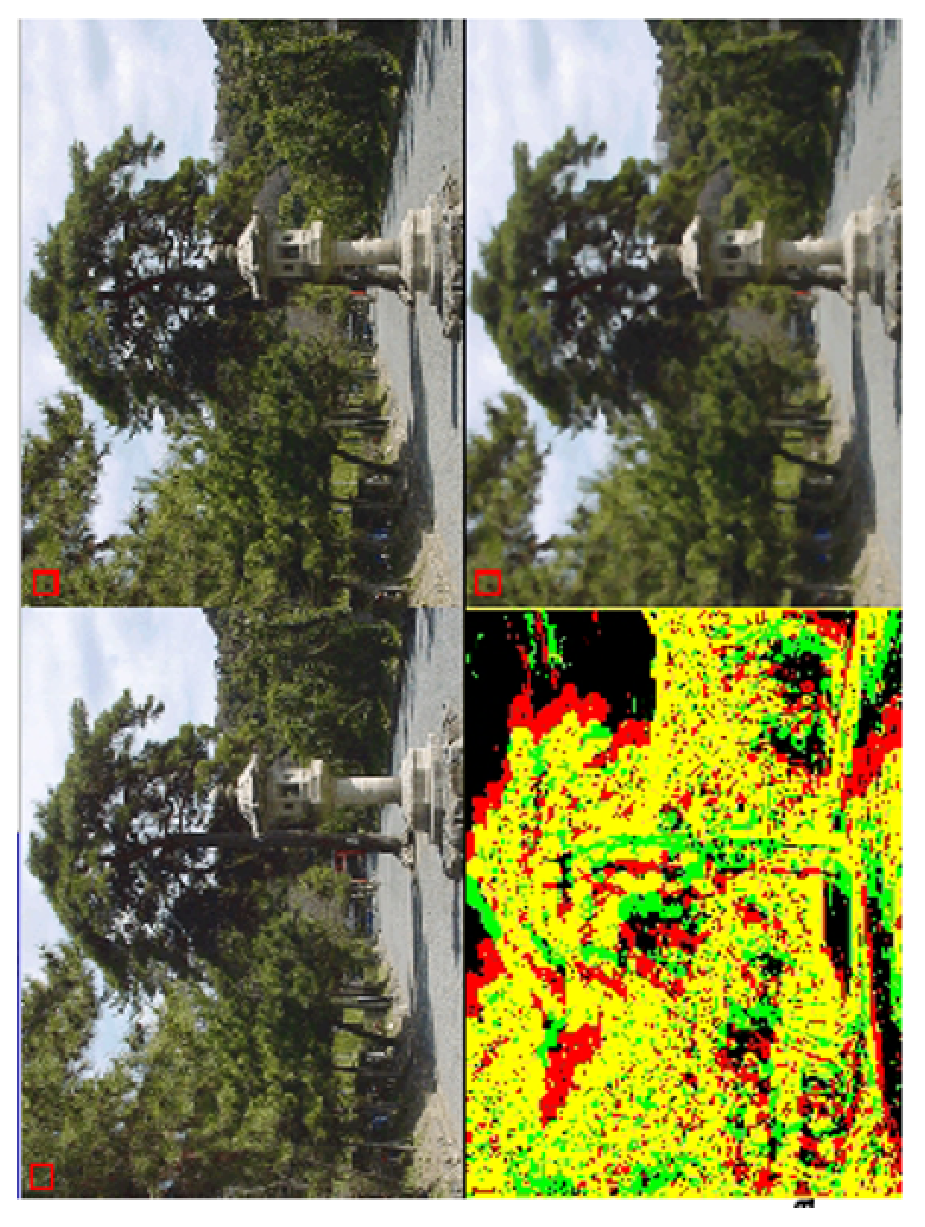
\includegraphics[angle=270,origin=b,width=0.75\textwidth]{edge.eps}
\caption{Edge}
\end{figure}

3x3�Υ��å����Хե��륿�Ǥ��롥���٤ΥС����ȱ黻�ˤ�ꡤ6�ս��OMAP=6�ˤγơ�
�ˤĤ��ơ�10��ʬ�Υե��륿������Ԥ���RMGRP=10�ˡ����ƥ󥷥�׻��Ǥ���
mapdist=1�Ǥ��롥

\begin{screen}
\tiny
\begin{verbatim}
void edge(Uint *p, struct E *r)
#if !defined(EMAX5) && !defined(EMAX6)
  for (top=PAD; top<HT-PAD; top++) { /* scan-lines */
    Uint  *p0 = p+(top  )*WD  ;
    Uint  *p1 = p+(top-1)*WD-1;
    Uint  *p2 = p+(top+1)*WD+1;
    Uint  *p3 = p+(top-1)*WD  ;
    Uint  *p4 = p+(top+1)*WD  ;
    Uint  *p5 = p+(top-1)*WD+1;
    Uint  *p6 = p+(top+1)*WD-1;
    Uint  *p7 = p+(top  )*WD-1;
    Uint  *p8 = p+(top  )*WD+1;
    Uchar *rp = r->E[top];
    for (cofs=0; cofs<WD; cofs++) {
      int d1 = df(*p1&MASK,*p2&MASK)+df(*p3&MASK,*p4&MASK)+df(*p5&MASK,*p6&MASK)+df(*p7&MASK,*p8&MASK);
      /* 0 < d1(42) < 256*2*4 */
      *rp = d1 < EDGEDET ? 0 : PIXMAX;
      p0++; p1++; p2++; p3++; p4++; p5++; p6++; p7++; p8++; rp++;
    }
  }
#endif
\end{verbatim}
\end{screen}

\begin{screen}
\tiny
\begin{verbatim}
  Ull  LOOP1, LOOP0;
  Ull  INIT1, INIT0;
  Ull  AR[64][4];                     /* output of EX     in each unit */
  Ull  BR[64][4][4];                  /* output registers in each unit */
  Ull  r0, r1, r2, r3, r4, r5, r6, r7, r8, r9, r10, r11, r12, r13, r14, r15;
  Ull  r16, r17, r18, r19, r20, r21, r22, r23, r24, r25, r26, r27, r28, r29, r30, r31;
  Ull  cc0, cc1, cc2, cc3, ex0, ex1;
  for (top=0; top<RRANGE; top+=RMGRP) { /* scan-lines */
    for (rofs=0; rofs<RMGRP; rofs++) { /* will be parallelized by multi-chip (M/#chip) */
      Uint *pp0[NCHIP], *pc0[NCHIP], *pn0[NCHIP]; Uchar *rc0[NCHIP];
      Uint *pp1[NCHIP], *pc1[NCHIP], *pn1[NCHIP]; Uchar *rc1[NCHIP];
      Uint *pp2[NCHIP], *pc2[NCHIP], *pn2[NCHIP]; Uchar *rc2[NCHIP];
      Uint *pp3[NCHIP], *pc3[NCHIP], *pn3[NCHIP]; Uchar *rc3[NCHIP];
      Uint *pp4[NCHIP], *pc4[NCHIP], *pn4[NCHIP]; Uchar *rc4[NCHIP];
      Uint *pp5[NCHIP], *pc5[NCHIP], *pn5[NCHIP]; Uchar *rc5[NCHIP];
      for (CHIP=0; CHIP<NCHIP; CHIP++) { /* will be parallelized by multi-chip (M/#chip) */
        int idx = (CHIP*RRANGE*OMAP+top+rofs)*WD;
        pp0[CHIP] = p+idx+RRANGE*WD*0-WD;  pc0[CHIP] = p+idx+RRANGE*WD*0; pn0[CHIP] = p+idx+RRANGE*WD*0+WD; rc0[CHIP] = (Uchar*)(r->E)+idx+RRANGE*WD*0;
        pp1[CHIP] = p+idx+RRANGE*WD*1-WD;  pc1[CHIP] = p+idx+RRANGE*WD*1; pn1[CHIP] = p+idx+RRANGE*WD*1+WD; rc1[CHIP] = (Uchar*)(r->E)+idx+RRANGE*WD*1;
        pp2[CHIP] = p+idx+RRANGE*WD*2-WD;  pc2[CHIP] = p+idx+RRANGE*WD*2; pn2[CHIP] = p+idx+RRANGE*WD*2+WD; rc2[CHIP] = (Uchar*)(r->E)+idx+RRANGE*WD*2;
        pp3[CHIP] = p+idx+RRANGE*WD*3-WD;  pc3[CHIP] = p+idx+RRANGE*WD*3; pn3[CHIP] = p+idx+RRANGE*WD*3+WD; rc3[CHIP] = (Uchar*)(r->E)+idx+RRANGE*WD*3;
        pp4[CHIP] = p+idx+RRANGE*WD*4-WD;  pc4[CHIP] = p+idx+RRANGE*WD*4; pn4[CHIP] = p+idx+RRANGE*WD*4+WD; rc4[CHIP] = (Uchar*)(r->E)+idx+RRANGE*WD*4;
        pp5[CHIP] = p+idx+RRANGE*WD*5-WD;  pc5[CHIP] = p+idx+RRANGE*WD*5; pn5[CHIP] = p+idx+RRANGE*WD*5+WD; rc5[CHIP] = (Uchar*)(r->E)+idx+RRANGE*WD*5;
      }
//EMAX5A begin edge mapdist=1
 /*2*/for (CHIP=0; CHIP<NCHIP; CHIP++) { /* output channels are parallelized by multi-chip (OC/#chip) */
   /*1*/for (INIT0=1,LOOP0=WD,cofs=0-4; LOOP0--; INIT0=0) {       /* stage#0 *//* mapped to FOR() on BR[63][0][0] */
 /*@0,1*/ exe(OP_ADD,       &cofs, cofs,        EXP_H3210, 4LL,  EXP_H3210, 0LL, EXP_H3210, OP_AND, 0x00000000ffffffffLL, OP_NOP, 0LL);
          /*map0*/
 /*@1,0*/ exe(OP_ADD,       &pofs, pc0[CHIP],   EXP_H3210, cofs, EXP_H3210, 0LL, EXP_H3210, OP_NOP,   0LL,    OP_NOP,  0LL);
 /*@2,0*/ mop(OP_LDWR, 1,   &r5,   pofs,       -1276, MSK_D0,    (Ull)pp0[CHIP],       WD,     0,   0,   (Ull)NULL,  WD);
 /*@2,0*/ mop(OP_LDWR, 1,   &r3,   pofs,       -1280, MSK_D0,    (Ull)pp0[CHIP],       WD,     0,   0,   (Ull)NULL,  WD);
 /*@2,1*/ mop(OP_LDWR, 1,   &r1,   pofs,       -1284, MSK_D0,    (Ull)pp0[CHIP],       WD,     0,   0,   (Ull)NULL,  WD);
 /*@3,0*/ exe(OP_NOP,    &AR[3][0],0LL,         EXP_H3210, 0LL,  EXP_H3210, 0LL, EXP_H3210, OP_OR,    0LL,    OP_NOP,  0LL);
 /*@3,0*/ mop(OP_LDWR, 1,   &r8,   pofs,           4, MSK_D0,    (Ull)pc0[CHIP],       WD,     0,   0,   (Ull)NULL,  WD);
 /*@3,0*/ mop(OP_LDWR, 1,   &r7,   pofs,          -4, MSK_D0,    (Ull)pc0[CHIP],       WD,     0,   0,   (Ull)NULL,  WD);
 /*@4,0*/ exe(OP_NOP,    &AR[4][0],0LL,         EXP_H3210, 0LL,  EXP_H3210, 0LL, EXP_H3210, OP_OR,    0LL,    OP_NOP,  0LL);
 /*@4,0*/ mop(OP_LDWR, 1,   &r2,   pofs,        1284, MSK_D0,    (Ull)pn0[CHIP],       WD,     0,   0,   (Ull)NULL,  WD);
 /*@4,0*/ mop(OP_LDWR, 1,   &r4,   pofs,        1280, MSK_D0,    (Ull)pn0[CHIP],       WD,     0,   0,   (Ull)NULL,  WD);
 /*@4,1*/ mop(OP_LDWR, 1,   &r6,   pofs,        1276, MSK_D0,    (Ull)pn0[CHIP],       WD,     0,   0,   (Ull)NULL,  WD);
 /*@4,1*/ exe(OP_MSSAD,     &r7,   0LL,         EXP_H3210, r7,   EXP_H3210, r8,  EXP_H3210, OP_NOP,   0LL,    OP_NOP,  0LL);
 /*@5,0*/ exe(OP_MSSAD,     &r1,   0LL,         EXP_H3210, r1,   EXP_H3210, r2,  EXP_H3210, OP_NOP,   0LL,    OP_NOP,  0LL);
 /*@5,1*/ exe(OP_MSSAD,     &r3,   0LL,         EXP_H3210, r3,   EXP_H3210, r4,  EXP_H3210, OP_NOP,   0LL,    OP_NOP,  0LL);
 /*@5,2*/ exe(OP_MSSAD,     &r5,   0LL,         EXP_H3210, r5,   EXP_H3210, r6,  EXP_H3210, OP_NOP,   0LL,    OP_NOP,  0LL);
 /*@6,0*/ exe(OP_MAUH,      &r1,   r3,          EXP_H3210, r1,   EXP_H3210, 0LL, EXP_H3210, OP_NOP,   0LL,    OP_NOP,  0LL);
 /*@6,1*/ exe(OP_MAUH,      &r5,   r7,          EXP_H3210, r5,   EXP_H3210, 0LL, EXP_H3210, OP_NOP,   0LL,    OP_NOP,  0LL);
 /*@7,0*/ exe(OP_MAUH,      &r1,   r5,          EXP_H3210, r1,   EXP_H3210, 0LL, EXP_H3210, OP_SUMHL, 0LL,    OP_NOP,  0LL);
 /*@8,0*/ exe(OP_MCAS,      &r31,  r1,          EXP_H3210, 64,   EXP_H3210, 0LL, EXP_H3210, OP_NOP,   0LL,    OP_NOP,  0LL);
 /*@8,0*/ mop(OP_STBR, 3,   &r31,  rc0[CHIP]++,    0, MSK_D0,    (Ull)rc0[CHIP],     WD/4,     0,   0,   (Ull)NULL,  WD/4);
     :
          /*map5*/
 /*@36,1*/exe(OP_ADD,       &pofs, pc5[CHIP],   EXP_H3210, cofs, EXP_H3210, 0LL, EXP_H3210, OP_NOP,   0LL,    OP_NOP,  0LL);
 /*@37,0*/mop(OP_LDWR, 1,   &r5,   pofs,       -1276, MSK_D0,    (Ull)pp5[CHIP],       WD,     0,   0,   (Ull)NULL,  WD);
 /*@37,0*/mop(OP_LDWR, 1,   &r3,   pofs,       -1280, MSK_D0,    (Ull)pp5[CHIP],       WD,     0,   0,   (Ull)NULL,  WD);
 /*@37,1*/mop(OP_LDWR, 1,   &r1,   pofs,       -1284, MSK_D0,    (Ull)pp5[CHIP],       WD,     0,   0,   (Ull)NULL,  WD);
 /*@38,0*/exe(OP_NOP,    &AR[38][0],0LL,        EXP_H3210, 0LL,  EXP_H3210, 0LL, EXP_H3210, OP_OR,    0LL,    OP_NOP,  0LL);
 /*@38,0*/mop(OP_LDWR, 1,   &r8,   pofs,           4, MSK_D0,    (Ull)pc5[CHIP],       WD,     0,   0,   (Ull)NULL,  WD);
 /*@38,0*/mop(OP_LDWR, 1,   &r7,   pofs,          -4, MSK_D0,    (Ull)pc5[CHIP],       WD,     0,   0,   (Ull)NULL,  WD);
 /*@39,0*/exe(OP_NOP,    &AR[39][0],0LL,        EXP_H3210, 0LL,  EXP_H3210, 0LL, EXP_H3210, OP_OR,    0LL,    OP_NOP,  0LL);
 /*@39,0*/mop(OP_LDWR, 1,   &r2,   pofs,        1284, MSK_D0,    (Ull)pn5[CHIP],       WD,     0,   0,   (Ull)NULL,  WD);
 /*@39,0*/mop(OP_LDWR, 1,   &r4,   pofs,        1280, MSK_D0,    (Ull)pn5[CHIP],       WD,     0,   0,   (Ull)NULL,  WD);
 /*@39,1*/mop(OP_LDWR, 1,   &r6,   pofs,        1276, MSK_D0,    (Ull)pn5[CHIP],       WD,     0,   0,   (Ull)NULL,  WD);
 /*@39,1*/exe(OP_MSSAD,     &r7,   0LL,         EXP_H3210, r7,   EXP_H3210, r8,  EXP_H3210, OP_NOP,   0LL,    OP_NOP,  0LL);
 /*@40,0*/exe(OP_MSSAD,     &r1,   0LL,         EXP_H3210, r1,   EXP_H3210, r2,  EXP_H3210, OP_NOP,   0LL,    OP_NOP,  0LL);
 /*@40,1*/exe(OP_MSSAD,     &r3,   0LL,         EXP_H3210, r3,   EXP_H3210, r4,  EXP_H3210, OP_NOP,   0LL,    OP_NOP,  0LL);
 /*@40,2*/exe(OP_MSSAD,     &r5,   0LL,         EXP_H3210, r5,   EXP_H3210, r6,  EXP_H3210, OP_NOP,   0LL,    OP_NOP,  0LL);
 /*@41,0*/exe(OP_MAUH,      &r1,   r3,          EXP_H3210, r1,   EXP_H3210, 0LL, EXP_H3210, OP_NOP,   0LL,    OP_NOP,  0LL);
 /*@41,1*/exe(OP_MAUH,      &r5,   r7,          EXP_H3210, r5,   EXP_H3210, 0LL, EXP_H3210, OP_NOP,   0LL,    OP_NOP,  0LL);
 /*@42,0*/exe(OP_MAUH,      &r1,   r5,          EXP_H3210, r1,   EXP_H3210, 0LL, EXP_H3210, OP_SUMHL, 0LL,    OP_NOP,  0LL);
 /*@43,0*/exe(OP_MCAS,      &r31,  r1,          EXP_H3210, 64,   EXP_H3210, 0LL, EXP_H3210, OP_NOP,   0LL,    OP_NOP,  0LL);
 /*@43,0*/mop(OP_STBR, 3,   &r31,  rc5[CHIP]++,    0, MSK_D0,    (Ull)rc5[CHIP],     WD/4,     0,   0,   (Ull)NULL,  WD/4);
        }
      }
//EMAX5A end
    }
  }
//EMAX5A drain_dirty_lmm
\end{verbatim}
\end{screen}

\begin{figure}[htbp]
\center
\epsfile{file=filter+rmm-edge-emax6.eps,width=1.00\textwidth}
\caption{Edge}
\end{figure}

\clearpage

\subsection{Stereo with stencil}

\begin{figure}[htbp]
\center
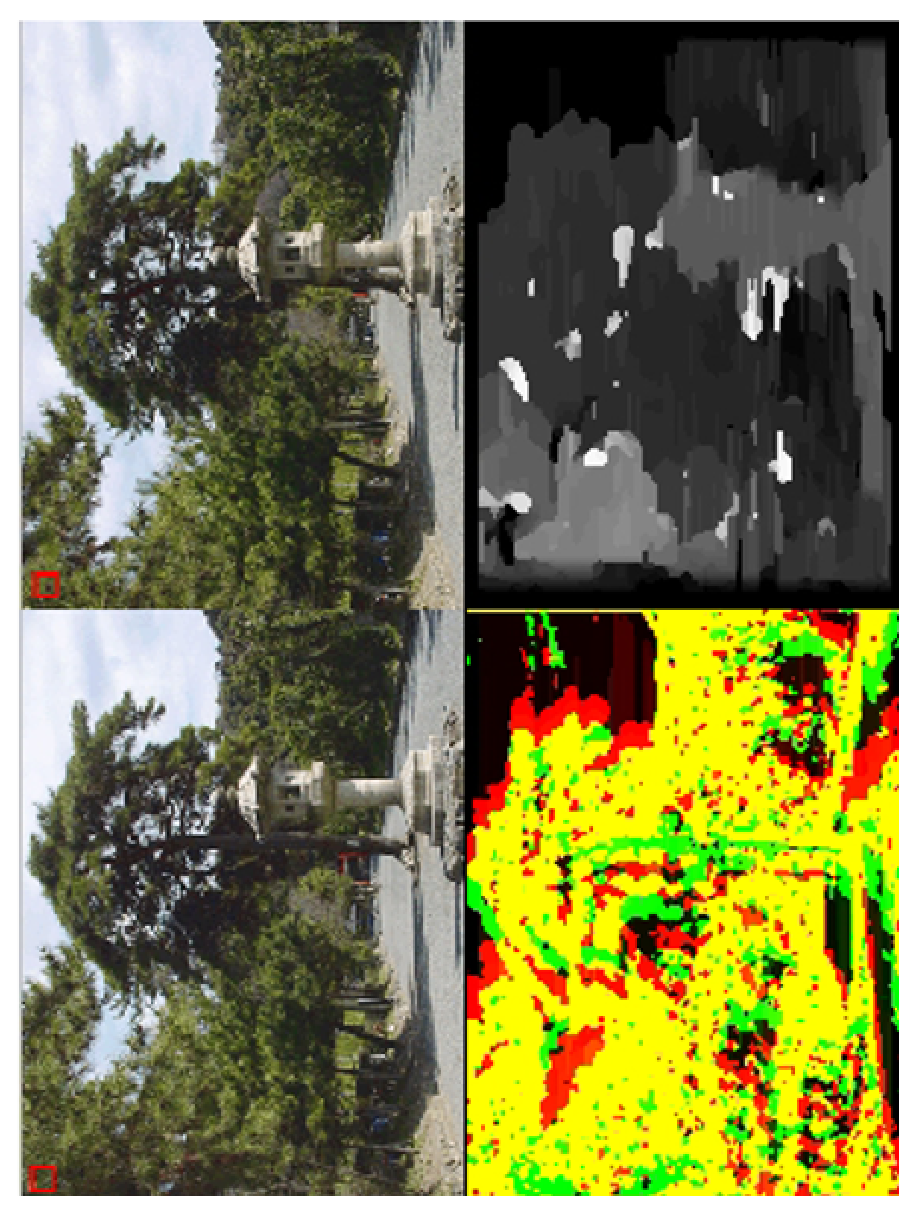
\includegraphics[angle=270,origin=b,width=0.75\textwidth]{stereo.eps}
\caption{Stereo}
\end{figure}

õ��������12x16�Υ��ƥ쥪�ޥå��󥰤Ǥ��롥���٤ΥС����ȱ黻�ˤ��8��ʬ��
SAD�򹹿����롥���ƥ󥷥�׻��ǤϤʤ���mapdist=0�Ǥ��롥

\begin{screen}
\tiny
\begin{verbatim}
void wdifline(Uint *l, Uint *r, struct SAD2 *d, int k)
#if !defined(EMAX5) && !defined(EMAX6)
  for (top=DWIN; top<HT-DWIN; top++) { /* scan-lines */
    for (cofs=DWIN+k/2; cofs<WD-DWIN-k/2; cofs++) /* one scan-line */
      d->SAD2[top][cofs] = 0;
  }

  for (top=DWIN; top<HT-DWIN; top++) { /* scan-lines */
    Uint *lp = l + top*WD+k; /* L */
    Uint *rp = r + top*WD; /* R */
    for (pofs1=-DWIN; pofs1<DWIN; pofs1++) {
      Uint *dp = &d->SAD2[top+pofs1][DWIN+k/2];
      for (cofs=0; cofs<WD-DWIN*2; cofs++) { /* one scan-line */
        int x, retval = 0;
        for (x=0; x<DWIN*2; x++)
          retval += df((*(lp+cofs+x))&MASK, (*(rp+cofs+x))&MASK);
        *(dp+cofs) += retval;
      }
    }
  }
#endif
\end{verbatim}
\end{screen}

\begin{screen}
\tiny
\begin{verbatim}
  for (top=0; top<RRANGE; top++) { /* will be parallelized by multi-chip (M/#chip) */
    for (CHIP=0; CHIP<NCHIP; CHIP++) { /* will be parallelized by multi-chip (M/#chip) */
      int idx = CHIP*RRANGE+DWIN+top;
      for (cofs=DWIN+k/2; cofs<WD-DWIN-k/2; cofs++) /* one scan-line */
        d->SAD2[idx][cofs] = 0;
    }
  }

  for (top=0; top<RRANGE; top++) { /* will be parallelized by multi-chip (M/#chip) */
    for (CHIP=0; CHIP<NCHIP; CHIP++) { /* will be parallelized by multi-chip (M/#chip) */
      int  idx = CHIP*RRANGE+DWIN+top;
      Uint *lp = l + idx*WD+k; /* L */
      Uint *rp = r + idx*WD; /* R */
      for (pofs1=-DWIN; pofs1<DWIN; pofs1++) {
        Uint *dp = &d->SAD2[idx+pofs1][DWIN+k/2];
        for (cofs=0; cofs<WD-DWIN*2; cofs++) { /* one scan-line */
          int x, retval = 0;
          for (x=0; x<DWIN*2; x++)
            retval += df((*(lp+cofs+x))&MASK, (*(rp+cofs+x))&MASK);
          *(dp+cofs) += retval;
        }
      }
    }
  }
\end{verbatim}
\end{screen}

\begin{screen}
\tiny
\begin{verbatim}
  Ull  LOOP1, LOOP0;  Ull  INIT1, INIT0;
  Ull  AR[64][4];                     /* output of EX     in each unit */
  Ull  BR[64][4][4];                  /* output registers in each unit */
  Ull  r0, r1, r2, r3, r4, r5, r6, r7, r8, r9, r10, r11, r12, r13, r14, r15;
  Ull  r16, r17, r18, r19, r20, r21, r22, r23, r24, r25, r26, r27, r28, r29, r30, r31;
  Ull  cc0, cc1, cc2, cc3, ex0, ex1;
  for (top=0; top<RRANGE; top++) { /* will be parallelized by multi-chip (M/#chip) */
    for (CHIP=0; CHIP<NCHIP; CHIP++) { /* will be parallelized by multi-chip (M/#chip) */
      int idx = CHIP*RRANGE+DWIN+top;
      for (cofs=DWIN+k/2; cofs<WD-DWIN-k/2; cofs++) /* one scan-line */
        d->SAD2[idx][cofs] = 0;
  } }
  for (top=0; top<RRANGE; top++) { /* scan-lines */
    Uint *lp[NCHIP],  *rp[NCHIP];
    Uint *dp0[NCHIP], *dp1[NCHIP], *dp2[NCHIP], *dp3[NCHIP], *dp4[NCHIP], *dp5[NCHIP], *dp6[NCHIP], *dp7[NCHIP];
    Uint *dp8[NCHIP], *dp9[NCHIP], *dpa[NCHIP], *dpb[NCHIP], *dpc[NCHIP], *dpd[NCHIP], *dpe[NCHIP], *dpf[NCHIP];
    for (CHIP=0; CHIP<NCHIP; CHIP++) { /* will be parallelized by multi-chip (M/#chip) */
      int idx = CHIP*RRANGE+DWIN+top;
      lp[CHIP] = l+idx*WD+k; rp[CHIP] = r+idx*WD;
      dp0[CHIP] = &d->SAD2[idx-8][DWIN+k/2];
      dp1[CHIP] = &d->SAD2[idx-7][DWIN+k/2];
      dp2[CHIP] = &d->SAD2[idx-6][DWIN+k/2];
        :
      dpf[CHIP] = &d->SAD2[idx+7][DWIN+k/2];
    }
//EMAX5A begin wdifline mapdist=0
 /*2*/for (CHIP=0; CHIP<NCHIP; CHIP++) { /* output channels are parallelized by multi-chip (OC/#chip) */
   /*1*/for (INIT0=1,LOOP0=WD,cofs=0-4; LOOP0--; INIT0=0) {       /* stage#0 *//* mapped to FOR() on BR[63][0][0] */
 /*@0,1*/ exe(OP_ADD,      &cofs,        cofs,        EXP_H3210, 4LL,  EXP_H3210, 0LL, EXP_H3210, OP_AND, 0x00000000ffffffffLL, OP_NOP, 0LL);
          /*map0*/
 /*@1,0*/ exe(OP_ADD,      &rofs1,       lp[CHIP],   EXP_H3210, cofs, EXP_H3210,    0, EXP_H3210, OP_NOP,  0LL,  OP_NOP,  0LL);
 /*@1,1*/ exe(OP_ADD,      &rofs2,       rp[CHIP],   EXP_H3210, cofs, EXP_H3210,    0, EXP_H3210, OP_NOP,  0LL,  OP_NOP,  0LL);
 /*@2,0*/ mop(OP_LDWR, 1,  &r2,          rofs1,   0,  MSK_D0,    lp[CHIP],       WD, 0, 0, (Ull)NULL,    WD);
 /*@2,0*/ mop(OP_LDWR, 1,  &r3,          rofs1,   4,  MSK_D0,    lp[CHIP],       WD, 0, 0, (Ull)NULL,    WD);
 /*@2,1*/ mop(OP_LDWR, 1,  &r4,          rofs1,   8,  MSK_D0,    lp[CHIP],       WD, 0, 0, (Ull)NULL,    WD);
 /*@2,1*/ mop(OP_LDWR, 1,  &r5,          rofs1,   12, MSK_D0,    lp[CHIP],       WD, 0, 0, (Ull)NULL,    WD);
 /*@2,2*/ mop(OP_LDWR, 1,  &r6,          rofs2,   0,  MSK_D0,    rp[CHIP],       WD, 0, 0, (Ull)NULL,    WD);
 /*@2,2*/ mop(OP_LDWR, 1,  &r7,          rofs2,   4,  MSK_D0,    rp[CHIP],       WD, 0, 0, (Ull)NULL,    WD);
 /*@2,3*/ mop(OP_LDWR, 1,  &r8,          rofs2,   8,  MSK_D0,    rp[CHIP],       WD, 0, 0, (Ull)NULL,    WD);
 /*@2,3*/ mop(OP_LDWR, 1,  &r9,          rofs2,   12, MSK_D0,    rp[CHIP],       WD, 0, 0, (Ull)NULL,    WD);
 /*@3,0*/ exe(OP_MSAD,     &r22,         r2,          EXP_H3210, r6,   EXP_H3210,    0, EXP_H3210, OP_NOP,  0LL,  OP_NOP,  0LL);
 /*@3,0*/ mop(OP_LDWR, 1,  &r12,         rofs1,   16, MSK_D0,    lp[CHIP],       WD, 0, 0, (Ull)NULL,    WD);
 /*@3,0*/ mop(OP_LDWR, 1,  &r13,         rofs1,   20, MSK_D0,    lp[CHIP],       WD, 0, 0, (Ull)NULL,    WD);
 /*@3,1*/ exe(OP_MSAD,     &r23,         r3,          EXP_H3210, r7,   EXP_H3210,    0, EXP_H3210, OP_NOP,  0LL,  OP_NOP,  0LL);
 /*@3,1*/ mop(OP_LDWR, 1,  &r14,         rofs1,   24, MSK_D0,    lp[CHIP],       WD, 0, 0, (Ull)NULL,    WD);
 /*@3,1*/ mop(OP_LDWR, 1,  &r15,         rofs1,   28, MSK_D0,    lp[CHIP],       WD, 0, 0, (Ull)NULL,    WD);
 /*@3,2*/ exe(OP_MSAD,     &r24,         r4,          EXP_H3210, r8,   EXP_H3210,    0, EXP_H3210, OP_NOP,  0LL,  OP_NOP,  0LL);
 /*@3,2*/ mop(OP_LDWR, 1,  &r16,         rofs2,   16, MSK_D0,    rp[CHIP],       WD, 0, 0, (Ull)NULL,    WD);
 /*@3,2*/ mop(OP_LDWR, 1,  &r17,         rofs2,   20, MSK_D0,    rp[CHIP],       WD, 0, 0, (Ull)NULL,    WD);
 /*@3,3*/ exe(OP_MSAD,     &r25,         r5,          EXP_H3210, r9,   EXP_H3210,    0, EXP_H3210, OP_NOP,  0LL,  OP_NOP,  0LL);
 /*@3,3*/ mop(OP_LDWR, 1,  &r18,         rofs2,   24, MSK_D0,    rp[CHIP],       WD, 0, 0, (Ull)NULL,    WD);
 /*@3,3*/ mop(OP_LDWR, 1,  &r19,         rofs2,   28, MSK_D0,    rp[CHIP],       WD, 0, 0, (Ull)NULL,    WD);
 /*@4,0*/ exe(OP_MSSAD,    &r12,         r22,         EXP_H3210, r12,  EXP_H3210,  r16, EXP_H3210, OP_NOP,  0LL,  OP_NOP,  0LL);
 /*@4,0*/ mop(OP_LDWR, 1,  &r2,          rofs1,   32, MSK_D0,    lp[CHIP],       WD, 0, 0, (Ull)NULL,    WD);
 /*@4,0*/ mop(OP_LDWR, 1,  &r3,          rofs1,   36, MSK_D0,    lp[CHIP],       WD, 0, 0, (Ull)NULL,    WD);
 /*@4,1*/ exe(OP_MSSAD,    &r13,         r23,         EXP_H3210, r13,  EXP_H3210,  r17, EXP_H3210, OP_NOP,  0LL,  OP_NOP,  0LL);
 /*@4,1*/ mop(OP_LDWR, 1,  &r4,          rofs1,   40, MSK_D0,    lp[CHIP],       WD, 0, 0, (Ull)NULL,    WD);
 /*@4,1*/ mop(OP_LDWR, 1,  &r5,          rofs1,   44, MSK_D0,    lp[CHIP],       WD, 0, 0, (Ull)NULL,    WD);
 /*@4,2*/ exe(OP_MSSAD,    &r14,         r24,         EXP_H3210, r14,  EXP_H3210,  r18, EXP_H3210, OP_NOP,  0LL,  OP_NOP,  0LL);
 /*@4,2*/ mop(OP_LDWR, 1,  &r6,          rofs2,   32, MSK_D0,    rp[CHIP],       WD, 0, 0, (Ull)NULL,    WD);
 /*@4,2*/ mop(OP_LDWR, 1,  &r7,          rofs2,   36, MSK_D0,    rp[CHIP],       WD, 0, 0, (Ull)NULL,    WD);
 /*@4,3*/ exe(OP_MSSAD,    &r15,         r25,         EXP_H3210, r15,  EXP_H3210,  r19, EXP_H3210, OP_NOP,  0LL,  OP_NOP,  0LL);
 /*@4,3*/ mop(OP_LDWR, 1,  &r8,          rofs2,   40, MSK_D0,    rp[CHIP],       WD, 0, 0, (Ull)NULL,    WD);
 /*@4,3*/ mop(OP_LDWR, 1,  &r9,          rofs2,   44, MSK_D0,    rp[CHIP],       WD, 0, 0, (Ull)NULL,    WD);
 /*@5,0*/ exe(OP_MSSAD,    &r22,         r12,         EXP_H3210, r2,   EXP_H3210,  r6, EXP_H3210, OP_NOP,  0LL,  OP_NOP,  0LL);
 /*@5,1*/ exe(OP_MSSAD,    &r23,         r13,         EXP_H3210, r3,   EXP_H3210,  r7, EXP_H3210, OP_NOP,  0LL,  OP_NOP,  0LL);
 /*@5,2*/ exe(OP_MSSAD,    &r24,         r14,         EXP_H3210, r4,   EXP_H3210,  r8, EXP_H3210, OP_NOP,  0LL,  OP_NOP,  0LL);
 /*@5,3*/ exe(OP_MSSAD,    &r25,         r15,         EXP_H3210, r5,   EXP_H3210,  r9, EXP_H3210, OP_NOP,  0LL,  OP_NOP,  0LL);
 /*@6,0*/ exe(OP_MAUH3,    &r31,         r22,         EXP_H3210, r23,  EXP_H3210, r24, EXP_H3210, OP_NOP,  0LL,  OP_NOP,  0LL);
 /*@7,0*/ exe(OP_MAUH3,    &r1,          r31,         EXP_H3210, r25,  EXP_H3210,   0, EXP_H3210, OP_SUMHL,0LL,  OP_NOP,  0LL);
 /*@8,0*/ mop(OP_LDWR, 1,  &BR[8][0][1], dp0[CHIP], cofs, MSK_D0, (Ull)dp0[CHIP], WD, 0, 1, (Ull)NULL,    WD);
 /*@8,0*/ exe(OP_ADD,      &AR[8][0],    BR[8][0][1], EXP_H3210, r1,   EXP_H3210,    0, EXP_H3210, OP_NOP,  0LL,  OP_NOP,  0LL);
 /*@8,0*/ mop(OP_STWR, 3,  &AR[8][0],    cofs, dp0[CHIP], MSK_D0, (Ull)dp0[CHIP], WD, 0, 1, (Ull)NULL,    WD);
          /*map1*/
 /*@9,0*/ mop(OP_LDWR, 1,  &BR[9][0][1], dp1[CHIP], cofs, MSK_D0, (Ull)dp1[CHIP], WD, 0, 1, (Ull)NULL,    WD);
 /*@9,0*/ exe(OP_ADD,      &AR[9][0],    BR[9][0][1], EXP_H3210, r1,   EXP_H3210,    0, EXP_H3210, OP_NOP,  0LL,  OP_NOP,  0LL);
 /*@9,0*/ mop(OP_STWR, 3,  &AR[9][0],    cofs, dp1[CHIP], MSK_D0, (Ull)dp1[CHIP], WD, 0, 1, (Ull)NULL,    WD);
          /*map2*/
 /*@10,0*/mop(OP_LDWR, 1,  &BR[10][0][1],dp2[CHIP], cofs, MSK_D0, (Ull)dp2[CHIP], WD, 0, 1, (Ull)NULL,    WD);
 /*@10,0*/exe(OP_ADD,      &AR[10][0],   BR[10][0][1], EXP_H3210,r1,   EXP_H3210,    0, EXP_H3210, OP_NOP,  0LL,  OP_NOP,  0LL);
 /*@10,0*/mop(OP_STWR, 3,  &AR[10][0],   cofs, dp2[CHIP], MSK_D0, (Ull)dp2[CHIP], WD, 0, 1, (Ull)NULL,    WD);
          :
          /*map9*/
 /*@17,0*/mop(OP_LDWR, 1,  &BR[17][0][1],dp9[CHIP], cofs, MSK_D0, (Ull)dp9[CHIP], WD, 0, 1, (Ull)NULL,    WD);
 /*@17,0*/exe(OP_ADD,      &AR[17][0],   BR[17][0][1], EXP_H3210,r1,   EXP_H3210,    0, EXP_H3210, OP_NOP,  0LL,  OP_NOP,  0LL);
 /*@17,0*/mop(OP_STWR, 3,  &AR[17][0],   cofs, dp9[CHIP], MSK_D0, (Ull)dp9[CHIP], WD, 0, 1, (Ull)NULL,    WD);
          /*map10*/
 /*@18,0*/mop(OP_LDWR, 1,  &BR[18][0][1],dpa[CHIP], cofs, MSK_D0, (Ull)dpa[CHIP], WD, 0, 1, (Ull)NULL,    WD);
 /*@18,0*/exe(OP_ADD,      &AR[18][0],   BR[18][0][1], EXP_H3210,r1,   EXP_H3210,    0, EXP_H3210, OP_NOP,  0LL,  OP_NOP,  0LL);
 /*@18,0*/mop(OP_STWR, 3,  &AR[18][0],   cofs, dpa[CHIP], MSK_D0, (Ull)dpa[CHIP], WD, 0, 1, (Ull)NULL,    WD);
          /*map11*/
 /*@19,0*/mop(OP_LDWR, 1,  &BR[19][0][1],dpb[CHIP], cofs, MSK_D0, (Ull)dpb[CHIP], WD, 0, 1, (Ull)NULL,    WD);
 /*@19,0*/exe(OP_ADD,      &AR[19][0],   BR[19][0][1], EXP_H3210,r1,   EXP_H3210,    0, EXP_H3210, OP_NOP,  0LL,  OP_NOP,  0LL);
 /*@19,0*/mop(OP_STWR, 3,  &AR[19][0],   cofs, dpb[CHIP], MSK_D0, (Ull)dpb[CHIP], WD, 0, 1, (Ull)NULL,    WD);
          /*map12*/
 /*@20,0*/mop(OP_LDWR, 1,  &BR[20][0][1],dpc[CHIP], cofs, MSK_D0, (Ull)dpc[CHIP], WD, 0, 1, (Ull)NULL,    WD);
 /*@20,0*/exe(OP_ADD,      &AR[20][0],   BR[20][0][1], EXP_H3210,r1,   EXP_H3210,    0, EXP_H3210, OP_NOP,  0LL,  OP_NOP,  0LL);
 /*@20,0*/mop(OP_STWR, 3,  &AR[20][0],   cofs, dpc[CHIP], MSK_D0, (Ull)dpc[CHIP], WD, 0, 1, (Ull)NULL,    WD);
          /*map13*/
 /*@21,0*/mop(OP_LDWR, 1,  &BR[21][0][1],dpd[CHIP], cofs, MSK_D0, (Ull)dpd[CHIP], WD, 0, 1, (Ull)NULL,    WD);
 /*@21,0*/exe(OP_ADD,      &AR[21][0],   BR[21][0][1], EXP_H3210,r1,   EXP_H3210,    0, EXP_H3210, OP_NOP,  0LL,  OP_NOP,  0LL);
 /*@21,0*/mop(OP_STWR, 3,  &AR[21][0],   cofs, dpd[CHIP], MSK_D0, (Ull)dpd[CHIP], WD, 0, 1, (Ull)NULL,    WD);
          /*map14*/
 /*@22,0*/mop(OP_LDWR, 1,  &BR[22][0][1],dpe[CHIP], cofs, MSK_D0, (Ull)dpe[CHIP], WD, 0, 1, (Ull)NULL,    WD);
 /*@22,0*/exe(OP_ADD,      &AR[22][0],   BR[22][0][1], EXP_H3210,r1,   EXP_H3210,    0, EXP_H3210, OP_NOP,  0LL,  OP_NOP,  0LL);
 /*@22,0*/mop(OP_STWR, 3,  &AR[22][0],   cofs, dpe[CHIP], MSK_D0, (Ull)dpe[CHIP], WD, 0, 1, (Ull)NULL,    WD);
          /*map15*/
 /*@23,0*/mop(OP_LDWR, 1,  &BR[23][0][1],dpf[CHIP], cofs, MSK_D0, (Ull)dpf[CHIP], WD, 0, 1, (Ull)NULL,    WD);
 /*@23,0*/exe(OP_ADD,      &AR[23][0],   BR[23][0][1], EXP_H3210,r1,   EXP_H3210,    0, EXP_H3210, OP_NOP,  0LL,  OP_NOP,  0LL);
 /*@23,0*/mop(OP_STWR, 3,  &AR[23][0],   cofs, dpf[CHIP], MSK_D0, (Ull)dpf[CHIP], WD, 0, 1, (Ull)NULL,    WD);
      } }
//EMAX5A end
  }
//EMAX5A drain_dirty_lmm
\end{verbatim}
\end{screen}

\begin{figure}[htbp]
\center
\epsfile{file=filter+rmm-wdifline-emax6.eps,width=1.00\textwidth}
\caption{Stereo with stencil}
\end{figure}

\clearpage

\section{3D-floating-point}

\shabox{
\leftline{cent\% make -f Makefile-csim.emax6+dma all clean}
\leftline{cent\% ../../src/csim/csim -x stencil-csim.emax6+dma}
}

\shabox{
\leftline{zynq\% make -f Makefile-zynq.emax6+dma all clean}
\leftline{zynq\% ./stencil-zynq.emax6+dma}
}

\subsection{Grapes with stencil}

\begin{figure}[htbp]
\center
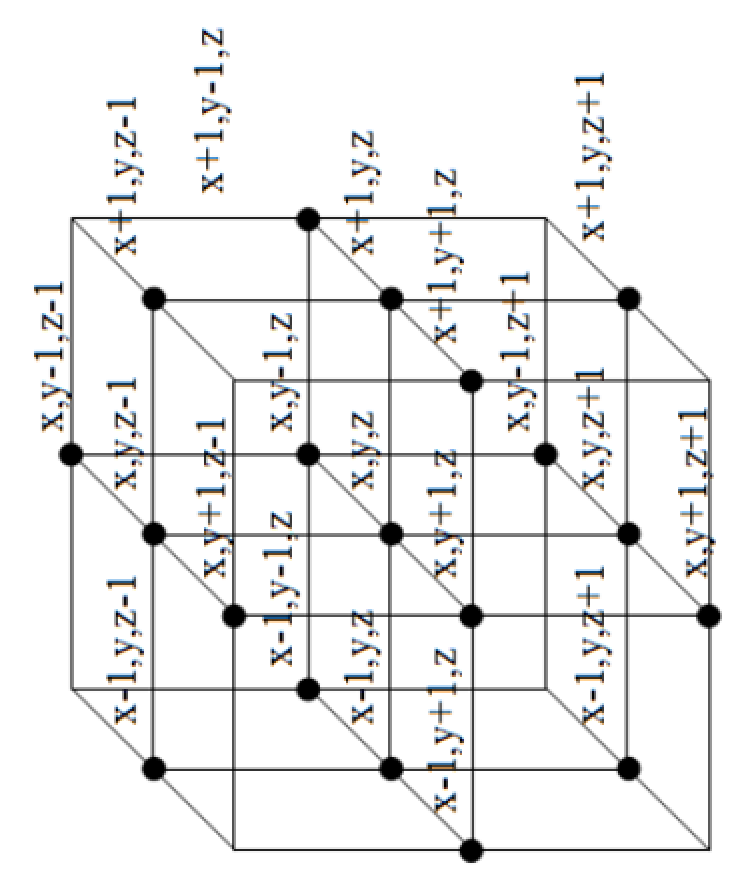
\includegraphics[angle=270,origin=b,width=0.30\textwidth]{grapes.eps}
\caption{Grapes}
\end{figure}

19����ư���������ƥ󥷥�׻��Ǥ��롥����A�˥��ƥ󥷥������ʤ���ΤΡ���ư��
���︺�Τ��ᡤ���٤ΥС����ȱ黻�ˤ��12��ʬ��׻������RMGRP=12�ˡ�����B��
�����Ѳ�ǽ�Ǥ��뤿��mapdist=1�Ǥ��롥

\begin{screen}
\tiny
\begin{verbatim}
grapes( float *c, float *a, float *b )
     /*C3D[DP][HT][WD]*/
     /*GrA[XC][DP][HT][WD]*/
     /*B3D[DP][HT][WD]*/
#define NCHIP     1
#define RMGRP     12
#define OMAP      1
#define PAD       1
#define RRANGE   ((HT-PAD*2)/NCHIP/OMAP)
  Ull  CHIP;
  Ull  LOOP1, LOOP0;
  Ull  INIT1, INIT0;
  Ull  AR[64][4];                     /* output of EX     in each unit */
  Ull  BR[64][4][4];                  /* output registers in each unit */
  Ull  r0, r1, r2, r3, r4, r5, r6, r7, r8, r9, r10, r11, r12, r13, r14, r15;
  Ull  r16, r17, r18, r19, r20, r21, r22, r23, r24, r25, r26, r27, r28, r29, r30, r31;
  Ull  cc0, cc1, cc2, cc3, ex0, ex1;
  int  x, y, z;
  int  row, col, n;
  Ull  roofs, coofs, aofs, bofs, cofs;

#if !defined(EMAX5) && !defined(EMAX6)
  for (z=PAD; z<DP-PAD; z++) {
    for (y=PAD; y<HT-PAD; y++) {
      for (x=PAD; x<WD-PAD; x++) {
        *(c+z*WDHT+y*WD+x) = *(b+(z-1)*WDHT+(y-1)*WD+x  ) * *(a+(MID-6)*WDHTDP+(z-1)*WDHT+(y-1)*WD+x  ) /* braw00 */ /* araw00 */
                           + *(b+(z-1)*WDHT+(y  )*WD+x-1) * *(a+(MID-5)*WDHTDP+(z-1)*WDHT+(y  )*WD+x-1) /* braw01 */ /* araw01 */
                           + *(b+(z-1)*WDHT+(y  )*WD+x  ) * *(a+(MID-4)*WDHTDP+(z-1)*WDHT+(y  )*WD+x  ) /* braw01 */ /* araw02 */
                           + *(b+(z-1)*WDHT+(y  )*WD+x+1) * *(a+(MID-5)*WDHTDP+(z-1)*WDHT+(y  )*WD+x+1) /* braw01 */ /* araw01 */
                           + *(b+(z-1)*WDHT+(y+1)*WD+x  ) * *(a+(MID-3)*WDHTDP+(z-1)*WDHT+(y+1)*WD+x  ) /* braw02 */ /* araw03 */
                           + *(b+(z  )*WDHT+(y-1)*WD+x-1) * *(a+(MID-2)*WDHTDP+(z  )*WDHT+(y-1)*WD+x-1) /* braw03 */ /* araw04 */
                           + *(b+(z  )*WDHT+(y-1)*WD+x  ) * *(a+(MID-1)*WDHTDP+(z  )*WDHT+(y-1)*WD+x  ) /* braw03 */ /* araw05 */
                           + *(b+(z  )*WDHT+(y-1)*WD+x+1) * *(a+(MID-2)*WDHTDP+(z  )*WDHT+(y-1)*WD+x+1) /* braw03 */ /* araw04 */
                           + *(b+(z  )*WDHT+(y  )*WD+x-1) * *(a+(MID  )*WDHTDP+(z  )*WDHT+(y  )*WD+x-1) /* braw04 */ /* araw06 */
                           + *(b+(z  )*WDHT+(y  )*WD+x  )                                               /* braw04 */
                           + *(b+(z  )*WDHT+(y  )*WD+x+1) * *(a+(MID  )*WDHTDP+(z  )*WDHT+(y  )*WD+x+1) /* braw04 */ /* araw06 */
                           + *(b+(z  )*WDHT+(y+1)*WD+x-1) * *(a+(MID+2)*WDHTDP+(z  )*WDHT+(y+1)*WD+x-1) /* braw05 */ /* araw08 */
                           + *(b+(z  )*WDHT+(y+1)*WD+x  ) * *(a+(MID+1)*WDHTDP+(z  )*WDHT+(y+1)*WD+x  ) /* braw05 */ /* araw07 */
                           + *(b+(z  )*WDHT+(y+1)*WD+x+1) * *(a+(MID+2)*WDHTDP+(z  )*WDHT+(y+1)*WD+x+1) /* braw05 */ /* araw08 */
                           + *(b+(z+1)*WDHT+(y-1)*WD+x  ) * *(a+(MID+3)*WDHTDP+(z+1)*WDHT+(y-1)*WD+x  ) /* braw06 */ /* araw09 */
                           + *(b+(z+1)*WDHT+(y  )*WD+x-1) * *(a+(MID+5)*WDHTDP+(z+1)*WDHT+(y  )*WD+x-1) /* braw07 */ /* araw0b */
                           + *(b+(z+1)*WDHT+(y  )*WD+x  ) * *(a+(MID+4)*WDHTDP+(z+1)*WDHT+(y  )*WD+x  ) /* braw07 */ /* araw0a */
                           + *(b+(z+1)*WDHT+(y  )*WD+x+1) * *(a+(MID+5)*WDHTDP+(z+1)*WDHT+(y  )*WD+x+1) /* braw07 */ /* araw0b */
                           + *(b+(z+1)*WDHT+(y+1)*WD+x  ) * *(a+(MID+6)*WDHTDP+(z+1)*WDHT+(y+1)*WD+x  );/* braw08 */ /* araw0c */
      }
    }
  }
#endif
\end{verbatim}
\end{screen}

\begin{screen}
\tiny
\begin{verbatim}
  for (z=PAD; z<DP-PAD; z++) {
    for (y=0; y<RRANGE; y+=RMGRP) {
      Ull  atop[NCHIP], btop[NCHIP], ctop[NCHIP];
      Ull  arow00[NCHIP], arow01[NCHIP], arow02[NCHIP], arow03[NCHIP], arow04[NCHIP], arow05[NCHIP], arow06[NCHIP], arow07[NCHIP], arow08[NCHIP],
           arow09[NCHIP], arow0a[NCHIP], arow0b[NCHIP], arow0c[NCHIP];
      Ull  brow00[NCHIP], brow01[NCHIP], brow02[NCHIP], brow03[NCHIP], brow04[NCHIP], brow05[NCHIP], brow06[NCHIP], brow07[NCHIP], brow08[NCHIP];
      Ull  crow0[NCHIP];
      for (CHIP=0; CHIP<NCHIP; CHIP++) { /* output channels are parallelized by multi-chip (OC/#chip) */
        atop[CHIP]   = a               +(z  )*WDHT+(CHIP*RRANGE*OMAP+RRANGE*0+PAD+y  )*WD;
        btop[CHIP]   = b               +(z  )*WDHT+(CHIP*RRANGE*OMAP+RRANGE*0+PAD+y  )*WD;
        ctop[CHIP]   = c               +(z  )*WDHT+(CHIP*RRANGE*OMAP+RRANGE*0+PAD+y  )*WD;
        arow00[CHIP] = a+(MID-6)*WDHTDP+(z-1)*WDHT+(CHIP*RRANGE*OMAP+RRANGE*0+PAD+y-1)*WD;
        arow01[CHIP] = a+(MID-5)*WDHTDP+(z-1)*WDHT+(CHIP*RRANGE*OMAP+RRANGE*0+PAD+y  )*WD;
        arow02[CHIP] = a+(MID-4)*WDHTDP+(z-1)*WDHT+(CHIP*RRANGE*OMAP+RRANGE*0+PAD+y  )*WD;
        arow03[CHIP] = a+(MID-3)*WDHTDP+(z-1)*WDHT+(CHIP*RRANGE*OMAP+RRANGE*0+PAD+y+1)*WD;
        arow04[CHIP] = a+(MID-2)*WDHTDP+(z  )*WDHT+(CHIP*RRANGE*OMAP+RRANGE*0+PAD+y-1)*WD;
        arow05[CHIP] = a+(MID-1)*WDHTDP+(z  )*WDHT+(CHIP*RRANGE*OMAP+RRANGE*0+PAD+y-1)*WD;
        arow06[CHIP] = a+(MID  )*WDHTDP+(z  )*WDHT+(CHIP*RRANGE*OMAP+RRANGE*0+PAD+y  )*WD;
        arow07[CHIP] = a+(MID+1)*WDHTDP+(z  )*WDHT+(CHIP*RRANGE*OMAP+RRANGE*0+PAD+y+1)*WD;
        arow08[CHIP] = a+(MID+2)*WDHTDP+(z  )*WDHT+(CHIP*RRANGE*OMAP+RRANGE*0+PAD+y+1)*WD;
        arow09[CHIP] = a+(MID+3)*WDHTDP+(z+1)*WDHT+(CHIP*RRANGE*OMAP+RRANGE*0+PAD+y-1)*WD;
        arow0a[CHIP] = a+(MID+4)*WDHTDP+(z+1)*WDHT+(CHIP*RRANGE*OMAP+RRANGE*0+PAD+y  )*WD;
        arow0b[CHIP] = a+(MID+5)*WDHTDP+(z+1)*WDHT+(CHIP*RRANGE*OMAP+RRANGE*0+PAD+y  )*WD;
        arow0c[CHIP] = a+(MID+6)*WDHTDP+(z+1)*WDHT+(CHIP*RRANGE*OMAP+RRANGE*0+PAD+y+1)*WD;
        brow00[CHIP] = b               +(z-1)*WDHT+(CHIP*RRANGE*OMAP+RRANGE*0+PAD+y-1)*WD;
        brow01[CHIP] = b               +(z-1)*WDHT+(CHIP*RRANGE*OMAP+RRANGE*0+PAD+y  )*WD;
        brow02[CHIP] = b               +(z-1)*WDHT+(CHIP*RRANGE*OMAP+RRANGE*0+PAD+y+1)*WD;
        brow03[CHIP] = b               +(z  )*WDHT+(CHIP*RRANGE*OMAP+RRANGE*0+PAD+y-1)*WD;
        brow04[CHIP] = b               +(z  )*WDHT+(CHIP*RRANGE*OMAP+RRANGE*0+PAD+y  )*WD;
        brow05[CHIP] = b               +(z  )*WDHT+(CHIP*RRANGE*OMAP+RRANGE*0+PAD+y+1)*WD;
        brow06[CHIP] = b               +(z+1)*WDHT+(CHIP*RRANGE*OMAP+RRANGE*0+PAD+y-1)*WD;
        brow07[CHIP] = b               +(z+1)*WDHT+(CHIP*RRANGE*OMAP+RRANGE*0+PAD+y  )*WD;
        brow08[CHIP] = b               +(z+1)*WDHT+(CHIP*RRANGE*OMAP+RRANGE*0+PAD+y+1)*WD;
        crow0[CHIP]  = c               +(z  )*WDHT+(CHIP*RRANGE*OMAP+RRANGE*0+PAD+y  )*WD;
      }
//EMAX5A begin grapes mapdist=1
      for (CHIP=0; CHIP<NCHIP; CHIP++) { /* output channels are parallelized by multi-chip (OC/#chip) */
   /*2*/for (INIT1=1,LOOP1=RMGRP,roofs=0-WD*4; LOOP1--; INIT1=0) {      /* stage#0 *//* mapped to FOR() on BR[63][1][0] */
     /*1*/for (INIT0=1,LOOP0=WD-PAD*2,coofs=(PAD-1)*4; LOOP0--; INIT0=0) {          /* stage#0 *//* mapped to FOR() on BR[63][0][0] */
            exe(OP_ADD,  &coofs, INIT0?coofs:coofs, EXP_H3210, 4, EXP_H3210, 0LL, EXP_H3210, OP_AND, 0x00000000ffffffffLL, OP_NOP, 0LL); /* stage#0 */
            exe(OP_ADD,  &roofs, roofs,  EXP_H3210, INIT0?WD*4:0, EXP_H3210, 0LL, EXP_H3210, OP_AND, 0x00000000ffffffffLL, OP_NOP, 0LL); /* stage#0 */
            exe(OP_ADD3, &aofs,  atop[CHIP], EXP_H3210, roofs, EXP_H3210,  coofs, EXP_H3210, OP_AND, 0x000000ffffffffffLL, OP_NOP, 0LL); /* stage#1 */
            exe(OP_ADD3, &bofs,  btop[CHIP], EXP_H3210, roofs, EXP_H3210,  coofs, EXP_H3210, OP_AND, 0x000000ffffffffffLL, OP_NOP, 0LL); /* stage#1 */
            exe(OP_ADD3, &cofs,  ctop[CHIP], EXP_H3210, roofs, EXP_H3210,  coofs, EXP_H3210, OP_AND, 0x000000ffffffffffLL, OP_NOP, 0LL); /* stage#1 */
            /*map0*/
            mop(OP_LDWR, 1, &BR[2][0][1], bofs, (0               -WDHT-WD  )*4, MSK_D0, brow00[CHIP], WD*(RMGRP+PAD*2), 0, 0, (Ull)NULL, WD*(RMGRP+PAD*2));/*st#2*/
            mop(OP_LDWR, 1, &BR[2][2][1], aofs, (0+WDHTDP*(MID-6)-WDHT-WD  )*4, MSK_D0, arow00[CHIP], WD*RMGRP, 0, 0, (Ull)NULL, WD*RMGRP);/* stage#2 */
            exe(OP_FML, &r0, BR[2][0][1], EXP_H3210,  BR[2][2][1], EXP_H3210, 0,           EXP_H3210, OP_NOP, 0LL, OP_NOP, 0LL);         /* stage#3 */
            mop(OP_LDWR, 1, &BR[3][0][1], bofs, (0               -WDHT   -1)*4, MSK_D0, brow00[CHIP], WD*(RMGRP+PAD*2), 0, 0, (Ull)NULL, WD*(RMGRP+PAD*2));/*st#3*/
            mop(OP_LDWR, 1, &BR[3][0][0], bofs, (0               -WDHT   +1)*4, MSK_D0, brow00[CHIP], WD*(RMGRP+PAD*2), 0, 0, (Ull)NULL, WD*(RMGRP+PAD*2));/*st#3*/
            mop(OP_LDWR, 1, &BR[3][1][1], bofs, (0               -WDHT     )*4, MSK_D0, brow00[CHIP], WD*(RMGRP+PAD*2), 0, 0, (Ull)NULL, WD*(RMGRP+PAD*2));/*st#3*/
            mop(OP_LDWR, 1, &BR[3][2][1], aofs, (0+WDHTDP*(MID-5)-WDHT   -1)*4, MSK_D0, arow01[CHIP], WD*RMGRP, 0, 0, (Ull)NULL, WD*RMGRP);/* stage#3 */
            mop(OP_LDWR, 1, &BR[3][2][0], aofs, (0+WDHTDP*(MID-5)-WDHT   +1)*4, MSK_D0, arow01[CHIP], WD*RMGRP, 0, 0, (Ull)NULL, WD*RMGRP);/* stage#3 */
            mop(OP_LDWR, 1, &BR[3][3][1], aofs, (0+WDHTDP*(MID-4)-WDHT     )*4, MSK_D0, arow02[CHIP], WD*RMGRP, 0, 0, (Ull)NULL, WD*RMGRP);/* stage#3 */
            exe(OP_FMA, &r1, r0,          EXP_H3210,  BR[3][0][1], EXP_H3210, BR[3][2][1], EXP_H3210, OP_NOP, 0LL, OP_NOP, 0LL);         /* stage#4 */
            exe(OP_FML, &r2, BR[3][0][0], EXP_H3210,  BR[3][2][0], EXP_H3210, 0,           EXP_H3210, OP_NOP, 0LL, OP_NOP, 0LL);         /* stage#4 */
            exe(OP_FML, &r3, BR[3][1][1], EXP_H3210,  BR[3][3][1], EXP_H3210, 0,           EXP_H3210, OP_NOP, 0LL, OP_NOP, 0LL);         /* stage#4 */
            mop(OP_LDWR, 1, &BR[4][0][1], bofs, (0               -WDHT+WD  )*4, MSK_D0, brow00[CHIP], WD*(RMGRP+PAD*2), 0, 0, (Ull)NULL, WD*(RMGRP+PAD*2));/*st#4*/
            mop(OP_LDWR, 1, &BR[4][2][1], aofs, (0+WDHTDP*(MID-3)-WDHT+WD  )*4, MSK_D0, arow03[CHIP], WD*RMGRP, 0, 0, (Ull)NULL, WD*RMGRP);/* stage#4 */
            exe(OP_FMA, &r4, r1,          EXP_H3210,  BR[4][0][1], EXP_H3210, BR[4][2][1], EXP_H3210, OP_NOP, 0LL, OP_NOP, 0LL);         /* stage#5 */
            exe(OP_FAD, &r5, r2,          EXP_H3210,  r3,          EXP_H3210, 0,           EXP_H3210, OP_NOP, 0LL, OP_NOP, 0LL);         /* stage#5 */

            mop(OP_LDWR, 1, &BR[6][0][1], bofs, (0                    -WD-1)*4, MSK_D0, brow03[CHIP], WD*(RMGRP+PAD*2), 0, 0, (Ull)NULL, WD*(RMGRP+PAD*2));/*st#6*/
            mop(OP_LDWR, 1, &BR[6][0][0], bofs, (0                    -WD+1)*4, MSK_D0, brow03[CHIP], WD*(RMGRP+PAD*2), 0, 0, (Ull)NULL, WD*(RMGRP+PAD*2));/*st#6*/
            mop(OP_LDWR, 1, &BR[6][1][1], bofs, (0                    -WD  )*4, MSK_D0, brow03[CHIP], WD*(RMGRP+PAD*2), 0, 0, (Ull)NULL, WD*(RMGRP+PAD*2));/*st#6*/
            mop(OP_LDWR, 1, &BR[6][2][1], aofs, (0+WDHTDP*(MID-2)     -WD-1)*4, MSK_D0, arow04[CHIP], WD*RMGRP, 0, 0, (Ull)NULL, WD*RMGRP);/* stage#6 */
            mop(OP_LDWR, 1, &BR[6][2][0], aofs, (0+WDHTDP*(MID-2)     -WD+1)*4, MSK_D0, arow04[CHIP], WD*RMGRP, 0, 0, (Ull)NULL, WD*RMGRP);/* stage#6 */
            mop(OP_LDWR, 1, &BR[6][3][1], aofs, (0+WDHTDP*(MID-1)     -WD  )*4, MSK_D0, arow05[CHIP], WD*RMGRP, 0, 0, (Ull)NULL, WD*RMGRP);/* stage#6 */
            exe(OP_FMA, &r0, r4,          EXP_H3210,  BR[6][0][1], EXP_H3210, BR[6][2][1], EXP_H3210, OP_NOP, 0LL, OP_NOP, 0LL);           /* stage#7 */
            exe(OP_FMA, &r1, r5,          EXP_H3210,  BR[6][0][0], EXP_H3210, BR[6][2][0], EXP_H3210, OP_NOP, 0LL, OP_NOP, 0LL);           /* stage#7 */
            exe(OP_FML, &r2, BR[6][1][1], EXP_H3210,  BR[6][3][1], EXP_H3210, 0,           EXP_H3210, OP_NOP, 0LL, OP_NOP, 0LL);           /* stage#7 */
            mop(OP_LDWR, 1, &BR[7][0][1], bofs, (0                       -1)*4, MSK_D0, brow03[CHIP], WD*(RMGRP+PAD*2), 0, 0, (Ull)NULL, WD*(RMGRP+PAD*2));/*st#7*/
            mop(OP_LDWR, 1, &BR[7][0][0], bofs, (0                       +1)*4, MSK_D0, brow03[CHIP], WD*(RMGRP+PAD*2), 0, 0, (Ull)NULL, WD*(RMGRP+PAD*2));/*st#7*/
            mop(OP_LDWR, 1, &BR[7][1][1], bofs, (0                         )*4, MSK_D0, brow03[CHIP], WD*(RMGRP+PAD*2), 0, 0, (Ull)NULL, WD*(RMGRP+PAD*2));/*st#7*/
            mop(OP_LDWR, 1, &BR[7][2][1], aofs, (0+WDHTDP*(MID  )        -1)*4, MSK_D0, arow06[CHIP], WD*RMGRP, 0, 0, (Ull)NULL, WD*RMGRP);/* stage#7 */
            mop(OP_LDWR, 1, &BR[7][2][0], aofs, (0+WDHTDP*(MID  )        +1)*4, MSK_D0, arow06[CHIP], WD*RMGRP, 0, 0, (Ull)NULL, WD*RMGRP);/* stage#7 */
            exe(OP_FMA, &r3, r0,          EXP_H3210,  BR[7][0][1], EXP_H3210, BR[7][2][1], EXP_H3210, OP_NOP, 0LL, OP_NOP, 0LL);           /* stage#8 */
            exe(OP_FMA, &r4, r1,          EXP_H3210,  BR[7][0][0], EXP_H3210, BR[7][2][0], EXP_H3210, OP_NOP, 0LL, OP_NOP, 0LL);           /* stage#8 */
            exe(OP_FAD, &r5, r2,          EXP_H3210,  BR[7][1][1], EXP_H3210, 0,           EXP_H3210, OP_NOP, 0LL, OP_NOP, 0LL);           /* stage#8 */
            mop(OP_LDWR, 1, &BR[8][0][1], bofs, (0                    +WD-1)*4, MSK_D0, brow03[CHIP], WD*(RMGRP+PAD*2), 0, 0, (Ull)NULL, WD*(RMGRP+PAD*2));/*st#8*/
            mop(OP_LDWR, 1, &BR[8][0][0], bofs, (0                    +WD+1)*4, MSK_D0, brow03[CHIP], WD*(RMGRP+PAD*2), 0, 0, (Ull)NULL, WD*(RMGRP+PAD*2));/*st#8*/
            mop(OP_LDWR, 1, &BR[8][1][1], bofs, (0                    +WD  )*4, MSK_D0, brow03[CHIP], WD*(RMGRP+PAD*2), 0, 0, (Ull)NULL, WD*(RMGRP+PAD*2));/*st#8*/
            mop(OP_LDWR, 1, &BR[8][2][1], aofs, (0+WDHTDP*(MID+2)     +WD-1)*4, MSK_D0, arow08[CHIP], WD*RMGRP, 0, 0, (Ull)NULL, WD*RMGRP);/* stage#8 */
            mop(OP_LDWR, 1, &BR[8][2][0], aofs, (0+WDHTDP*(MID+2)     +WD+1)*4, MSK_D0, arow08[CHIP], WD*RMGRP, 0, 0, (Ull)NULL, WD*RMGRP);/* stage#8 */
            mop(OP_LDWR, 1, &BR[8][3][1], aofs, (0+WDHTDP*(MID+1)     +WD  )*4, MSK_D0, arow07[CHIP], WD*RMGRP, 0, 0, (Ull)NULL, WD*RMGRP);/* stage#8 */
            exe(OP_FMA, &r6, r3,          EXP_H3210,  BR[8][0][1], EXP_H3210, BR[8][2][1], EXP_H3210, OP_NOP, 0LL, OP_NOP, 0LL);           /* stage#9 */
            exe(OP_FMA, &r7, r4,          EXP_H3210,  BR[8][0][0], EXP_H3210, BR[8][2][0], EXP_H3210, OP_NOP, 0LL, OP_NOP, 0LL);           /* stage#9 */
            exe(OP_FMA, &r8, r5,          EXP_H3210,  BR[8][1][1], EXP_H3210, BR[8][3][1], EXP_H3210, OP_NOP, 0LL, OP_NOP, 0LL);           /* stage#9 */

            mop(OP_LDWR, 1, &BR[10][0][1],bofs, (0               +WDHT-WD  )*4, MSK_D0, brow06[CHIP], WD*(RMGRP+PAD*2), 0, 0, (Ull)NULL, WD*(RMGRP+PAD*2));/*st#10*/
            mop(OP_LDWR, 1, &BR[10][2][1],aofs, (0+WDHTDP*(MID+3)+WDHT-WD  )*4, MSK_D0, arow09[CHIP], WD*RMGRP, 0, 0, (Ull)NULL, WD*RMGRP);/* stage#10*/
            exe(OP_FMA, &r0, r6,          EXP_H3210,  BR[10][0][1],EXP_H3210, BR[10][2][1],EXP_H3210, OP_NOP, 0LL, OP_NOP, 0LL);           /* stage#11*/
            exe(OP_FAD, &r1, r7,          EXP_H3210,  r8,          EXP_H3210, 0,           EXP_H3210, OP_NOP, 0LL, OP_NOP, 0LL);           /* stage#11*/
            mop(OP_LDWR, 1, &BR[11][0][1],bofs, (0               +WDHT   -1)*4, MSK_D0, brow06[CHIP], WD*(RMGRP+PAD*2), 0, 0, (Ull)NULL, WD*(RMGRP+PAD*2));/*st#11*/
            mop(OP_LDWR, 1, &BR[11][0][0],bofs, (0               +WDHT   +1)*4, MSK_D0, brow06[CHIP], WD*(RMGRP+PAD*2), 0, 0, (Ull)NULL, WD*(RMGRP+PAD*2));/*st#11*/
            mop(OP_LDWR, 1, &BR[11][1][1],bofs, (0               +WDHT     )*4, MSK_D0, brow06[CHIP], WD*(RMGRP+PAD*2), 0, 0, (Ull)NULL, WD*(RMGRP+PAD*2));/*st#11*/
            mop(OP_LDWR, 1, &BR[11][2][1],aofs, (0+WDHTDP*(MID+5)+WDHT   -1)*4, MSK_D0, arow0b[CHIP], WD*RMGRP, 0, 0, (Ull)NULL, WD*RMGRP);/* stage#11*/
            mop(OP_LDWR, 1, &BR[11][2][0],aofs, (0+WDHTDP*(MID+5)+WDHT   +1)*4, MSK_D0, arow0b[CHIP], WD*RMGRP, 0, 0, (Ull)NULL, WD*RMGRP);/* stage#11*/
            mop(OP_LDWR, 1, &BR[11][3][1],aofs, (0+WDHTDP*(MID+4)+WDHT     )*4, MSK_D0, arow0a[CHIP], WD*RMGRP, 0, 0, (Ull)NULL, WD*RMGRP);/* stage#11*/
            exe(OP_FMA, &r2, r0,          EXP_H3210,  BR[11][0][1],EXP_H3210, BR[11][2][1],EXP_H3210, OP_NOP, 0LL, OP_NOP, 0LL);           /* stage#12*/
            exe(OP_FMA, &r3, r1,          EXP_H3210,  BR[11][0][0],EXP_H3210, BR[11][2][0],EXP_H3210, OP_NOP, 0LL, OP_NOP, 0LL);           /* stage#12*/
            exe(OP_FML, &r4, BR[11][1][1],EXP_H3210,  BR[11][3][1],EXP_H3210, 0,           EXP_H3210, OP_NOP, 0LL, OP_NOP, 0LL);           /* stage#12*/
            mop(OP_LDWR, 1, &BR[12][0][1],bofs, (0               +WDHT+WD  )*4, MSK_D0, brow06[CHIP], WD*(RMGRP+PAD*2), 0, 0, (Ull)NULL, WD*(RMGRP+PAD*2));/*st#12*/
            mop(OP_LDWR, 1, &BR[12][2][1],aofs, (0+WDHTDP*(MID+6)+WDHT+WD  )*4, MSK_D0, arow0c[CHIP], WD*RMGRP, 0, 0, (Ull)NULL, WD*RMGRP);/* stage#12*/
            exe(OP_FMA, &r5, r2,          EXP_H3210,  BR[12][0][1],EXP_H3210, BR[12][2][1],EXP_H3210, OP_NOP, 0LL, OP_NOP, 0LL);           /* stage#13*/
            exe(OP_FAD, &r6, r3,          EXP_H3210,  r4,          EXP_H3210, 0,           EXP_H3210, OP_NOP, 0LL, OP_NOP, 0LL);           /* stage#13*/
            exe(OP_FAD, &r7, r5,          EXP_H3210,  r6,          EXP_H3210, 0,           EXP_H3210, OP_NOP, 0LL, OP_NOP, 0LL);           /* stage#14*/
            mop(OP_STWR, 3, &r7,          cofs, (0                         )*4, MSK_D0, crow0[CHIP],  WD*RMGRP, 0, 0, (Ull)NULL, WD*RMGRP);/* stage#14*/
          }
        }
      }
//EMAX5A end
    }
//EMAX5A drain_dirty_lmm
  }
\end{verbatim}
\end{screen}

\begin{figure}[htbp]
\center
\epsfile{file=stencil+rmm-grapes-emax6.eps,width=1.00\textwidth}
\caption{Grapes}
\end{figure}

\clearpage

\subsection{Jacobi with stencil}

\begin{figure}[htbp]
\center
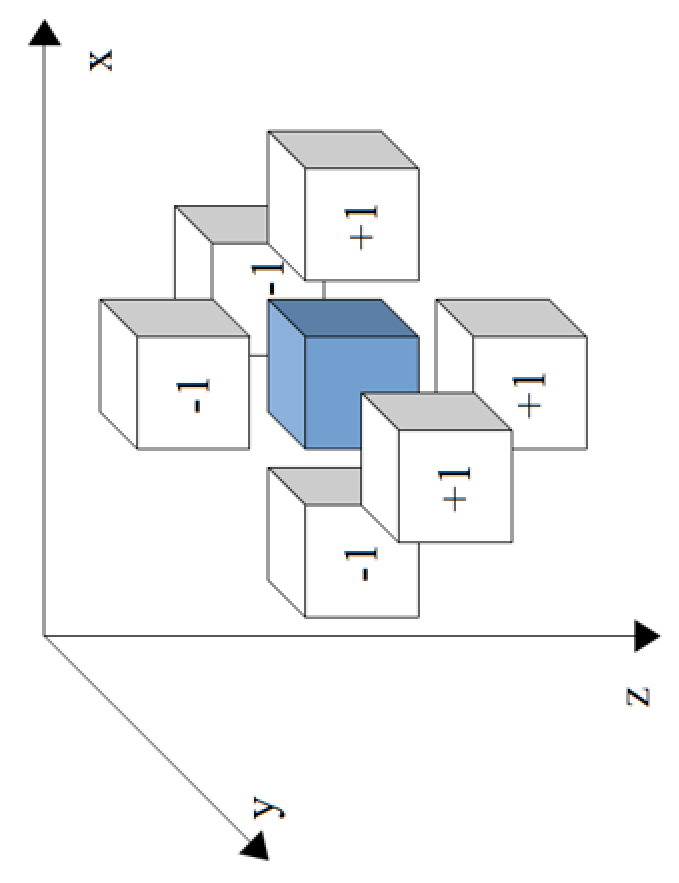
\includegraphics[angle=270,origin=b,width=0.75\textwidth]{jacobi.eps}
\caption{Jacobi}
\end{figure}

7����ư���������ƥ󥷥�׻��Ǥ��롥���٤ΥС����ȱ黻�ˤ��24��ʬ��׻�����
��RMGRP=24�ˡ����ƥ󥷥�׻��Ǥ����ΤΡ����٤�24��ʬ��׻����뤿�ᡤ
mapdist=0�Ǥ��롥

\begin{screen}
\tiny
\begin{verbatim}
jacobi( float *c, float *b )
     /*C3D[DP][HT][WD]*/
     /*B3D[DP][HT][WD]*/
#undef  NCHIP
#undef  RMGRP
#undef  OMAP
#undef  PAD
#undef  RRANGE
#define NCHIP     1
#define RMGRP     24
#define OMAP      1
#define PAD       1
#define RRANGE   ((HT-PAD*2)/NCHIP/OMAP)
  Ull  CHIP;
  Ull  LOOP1, LOOP0;
  Ull  INIT1, INIT0;
  Ull  AR[64][4];                     /* output of EX     in each unit */
  Ull  BR[64][4][4];                  /* output registers in each unit */
  Ull  r0, r1, r2, r3, r4, r5, r6, r7, r8, r9, r10, r11, r12, r13, r14, r15;
  Ull  r16, r17, r18, r19, r20, r21, r22, r23, r24, r25, r26, r27, r28, r29, r30, r31;
  Ull  cc0, cc1, cc2, cc3, ex0, ex1;
  int  x, y, z;
  int  row, col, n;
  Ull  roofs, coofs, aofs, bofs, cofs;
  union {float f; int i;} C1, C2;
  C1.f = 0.2;
  C2.f = 0.3;
  Ull  I1 = C1.i;
  Ull  I2 = C2.i;

#if !defined(EMAX5) && !defined(EMAX6)
  for (z=PAD; z<DP-PAD; z++) {
    for (y=PAD; y<HT-PAD; y++) {
      for (x=PAD; x<WD-PAD; x++) {
        *(c+z*WDHT+y*WD+x) = C2.f *(*(b+(z-1)*WDHT+(y  )*WD+x  )
                                  + *(b+(z  )*WDHT+(y-1)*WD+x  )
                                  + *(b+(z  )*WDHT+(y  )*WD+x-1)
                                  + *(b+(z  )*WDHT+(y  )*WD+x+1)
                                  + *(b+(z  )*WDHT+(y+1)*WD+x  )
                                  + *(b+(z+1)*WDHT+(y  )*WD+x  ))
                           + C1.f * *(b+(z  )*WDHT+(y  )*WD+x  );
      }
    }
  }
#endif
\end{verbatim}
\end{screen}

\begin{screen}
\tiny
\begin{verbatim}
  for (z=PAD; z<DP-PAD; z++) {
    for (y=0; y<RRANGE; y+=RMGRP) {
      Ull  btop[NCHIP], ctop[NCHIP];
      Ull  brow00[NCHIP], brow01[NCHIP], brow02[NCHIP], brow03[NCHIP], brow04[NCHIP];
      Ull  crow0[NCHIP];
      for (CHIP=0; CHIP<NCHIP; CHIP++) { /* output channels are parallelized by multi-chip (OC/#chip) */
        btop[CHIP]   = b               +(z  )*WDHT+(CHIP*RRANGE*OMAP+RRANGE*0+PAD+y  )*WD;
        ctop[CHIP]   = c               +(z  )*WDHT+(CHIP*RRANGE*OMAP+RRANGE*0+PAD+y  )*WD;
        brow00[CHIP] = b               +(z-1)*WDHT+(CHIP*RRANGE*OMAP+RRANGE*0+PAD+y  )*WD;
        brow01[CHIP] = b               +(z+1)*WDHT+(CHIP*RRANGE*OMAP+RRANGE*0+PAD+y  )*WD;
        brow02[CHIP] = b               +(z  )*WDHT+(CHIP*RRANGE*OMAP+RRANGE*0+PAD+y-1)*WD;
        brow03[CHIP] = b               +(z  )*WDHT+(CHIP*RRANGE*OMAP+RRANGE*0+PAD+y  )*WD;/* not used for RMGRP>1 */
        brow04[CHIP] = b               +(z  )*WDHT+(CHIP*RRANGE*OMAP+RRANGE*0+PAD+y+1)*WD;/* not used for RMGRP>1 */
        crow0[CHIP]  = c               +(z  )*WDHT+(CHIP*RRANGE*OMAP+RRANGE*0+PAD+y  )*WD;
      }
//EMAX5A begin jacobi mapdist=0 /* 7 PAD>0�ξ��,PLOAD��LOAD�ΰ褬������ʣ.load���LMM�ˤ�PLOAD������ि��˽��ڤ�ȯ������ */
      for (CHIP=0; CHIP<NCHIP; CHIP++) { /* output channels are parallelized by multi-chip (OC/#chip) */
   /*2*/for (INIT1=1,LOOP1=RMGRP,roofs=0-WD*4; LOOP1--; INIT1=0) {      /* stage#0 *//* mapped to FOR() on BR[63][1][0] */
     /*1*/for (INIT0=1,LOOP0=WD-PAD*2,coofs=(PAD-1)*4; LOOP0--; INIT0=0) {          /* stage#0 *//* mapped to FOR() on BR[63][0][0] */
            exe(OP_ADD,  &coofs, INIT0?coofs:coofs, EXP_H3210, 4, EXP_H3210, 0LL, EXP_H3210, OP_AND, 0x00000000ffffffffLL, OP_NOP, 0LL); /* stage#0 */
            exe(OP_ADD,  &roofs, roofs,  EXP_H3210, INIT0?WD*4:0, EXP_H3210, 0LL, EXP_H3210, OP_AND, 0x00000000ffffffffLL, OP_NOP, 0LL); /* stage#0 */
            exe(OP_ADD3, &bofs,  btop[CHIP], EXP_H3210, roofs, EXP_H3210,  coofs, EXP_H3210, OP_AND, 0x000000ffffffffffLL, OP_NOP, 0LL); /* stage#1 */
            exe(OP_ADD3, &cofs,  ctop[CHIP], EXP_H3210, roofs, EXP_H3210,  coofs, EXP_H3210, OP_AND, 0x000000ffffffffffLL, OP_NOP, 0LL); /* stage#1 */
            /*map0*/
            mop(OP_LDWR, 1, &BR[2][0][1], bofs, (0        -WDHT     )*4, MSK_D0, brow00[CHIP], WD*RMGRP, 0, 0, NULL, WD*RMGRP);      /* stage#2 */
            mop(OP_LDWR, 1, &BR[2][2][1], bofs, (0        +WDHT     )*4, MSK_D0, brow01[CHIP], WD*RMGRP, 0, 0, CHIP]*/NULL, WD*RMGRP); /* stage#2 */
            exe(OP_FAD, &r0, BR[2][0][1],EXP_H3210,  BR[2][2][1],EXP_H3210, 0,           EXP_H3210, OP_NOP, 0LL, OP_NOP, 0LL);           /* stage#3 */
            mop(OP_LDWR, 1, &BR[3][0][1], bofs, (0             -WD  )*4, MSK_D0, brow02[CHIP], WD*(RMGRP+PAD*2), 0, 0, NULL, WD*(RMGRP+PAD*2)); /* stage#3 */
            exe(OP_FAD, &r1, r0,         EXP_H3210,  BR[3][0][1],EXP_H3210, 0,           EXP_H3210, OP_NOP, 0LL, OP_NOP, 0LL);           /* stage#3 */
            mop(OP_LDWR, 1, &BR[4][0][1], bofs, (0                -1)*4, MSK_D0, brow02[CHIP], WD*(RMGRP+PAD*2), 0, 0, NULL, WD*(RMGRP+PAD*2)); /* stage#4 */
            mop(OP_LDWR, 1, &BR[4][1][1], bofs, (0                  )*4, MSK_D0, brow02[CHIP], WD*(RMGRP+PAD*2), 0, 0, NULL, WD*(RMGRP+PAD*2)); /* stage#4 */
            mop(OP_LDWR, 1, &BR[4][2][1], bofs, (0                +1)*4, MSK_D0, brow02[CHIP], WD*(RMGRP+PAD*2), 0, 0, NULL, WD*(RMGRP+PAD*2)); /* stage#4 */
            exe(OP_FAD, &r2, r1,         EXP_H3210,  BR[4][0][1],EXP_H3210, 0,           EXP_H3210, OP_NOP, 0LL, OP_NOP, 0LL);           /* stage#5 */
            exe(OP_FML, &r3, I1,         EXP_H3210,  BR[4][1][1],EXP_H3210, 0,           EXP_H3210, OP_NOP, 0LL, OP_NOP, 0LL);           /* stage#5 */
            mop(OP_LDWR, 1, &BR[5][0][1], bofs, (0             +WD  )*4, MSK_D0, brow02[CHIP], WD*(RMGRP+PAD*2), 0, 0, NULL, WD*(RMGRP+PAD*2)); /* stage#5 */
            exe(OP_FAD, &r4, r2,         EXP_H3210,  BR[5][0][1],EXP_H3210, 0,           EXP_H3210, OP_NOP, 0LL, OP_NOP, 0LL);           /* stage#6 */
            exe(OP_FAD, &r5, r4,         EXP_H3210,  BR[4][2][1],EXP_H3210, 0,           EXP_H3210, OP_NOP, 0LL, OP_NOP, 0LL);           /* stage#7 */
            exe(OP_FMA, &r6, r3,         EXP_H3210,  r5,         EXP_H3210, I2,          EXP_H3210, OP_NOP, 0LL, OP_NOP, 0LL);           /* stage#8 */
            mop(OP_STWR, 3, &r6,          cofs, (0                  )*4, MSK_D0, crow0[CHIP],  WD*RMGRP, 0, 0, /NULL, WD*RMGRP);     /* stage#8 */
          }
        }
      }
//EMAX5A end
    }
//EMAX5A drain_dirty_lmm
  }
\end{verbatim}
\end{screen}

\begin{figure}[htbp]
\center
\epsfile{file=stencil+rmm-jacobi-emax6.eps,width=1.00\textwidth}
\caption{Jacobi}
\end{figure}

\clearpage

\subsection{Fd6 with stencil}

\begin{figure}[htbp]
\center
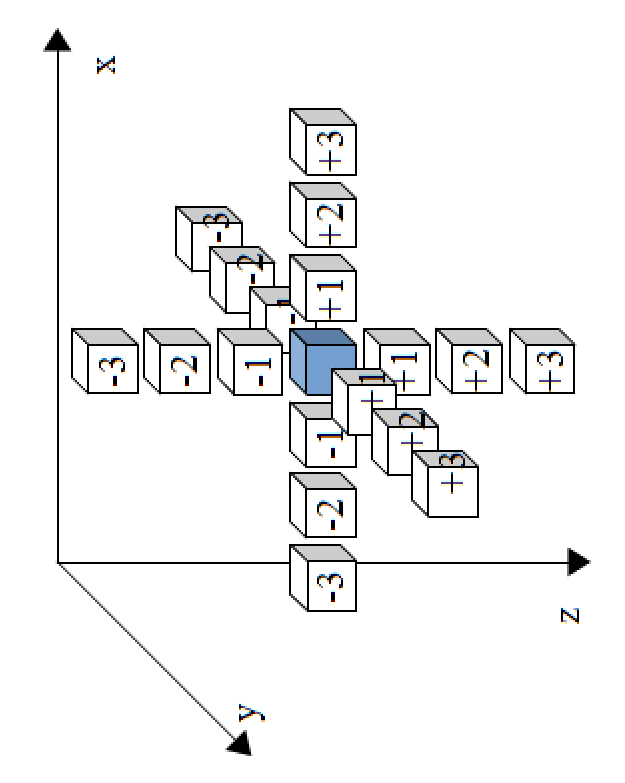
\includegraphics[angle=270,origin=b,width=0.60\textwidth]{fd6.eps}
\caption{Fd6}
\end{figure}

����3��19����ư���������ƥ󥷥�׻��Ǥ��롥���٤ΥС����ȱ黻�ˤ��24��ʬ��
�׻������RMGRP=24�ˡ����ƥ󥷥�׻��Ǥ����ΤΡ����٤�24��ʬ��׻����뤿�ᡤ
mapdist=0�Ǥ��롥

\begin{screen}
\tiny
\begin{verbatim}
fd6( float *c, float *b )
     /*C3D[DP][HT][WD]*/
     /*B3D[DP][HT][WD]*/
#define NCHIP     1
#define RMGRP     24
#define OMAP      1
#define PAD       3
#define RRANGE   ((HT-PAD*2)/NCHIP/OMAP)
  Ull  CHIP;
  Ull  LOOP1, LOOP0;
  Ull  INIT1, INIT0;
  Ull  AR[64][4];                     /* output of EX     in each unit */
  Ull  BR[64][4][4];                  /* output registers in each unit */
  Ull  r0, r1, r2, r3, r4, r5, r6, r7, r8, r9, r10, r11, r12, r13, r14, r15;
  Ull  r16, r17, r18, r19, r20, r21, r22, r23, r24, r25, r26, r27, r28, r29, r30, r31;
  Ull  cc0, cc1, cc2, cc3, ex0, ex1;
  int  x, y, z;
  int  row, col, n;
  Ull  roofs, coofs, aofs, bofs, cofs;
  union {float f; int i;} C1, C2, C3, C4;
  C1.f = 0.1;
  C2.f = 0.2;
  C3.f = 0.4;
  C4.f = 0.8;
  Ull  I1 = C1.i;
  Ull  I2 = C2.i;
  Ull  I3 = C3.i;
  Ull  I4 = C4.i;

#if !defined(EMAX5) && !defined(EMAX6)
  for (z=PAD; z<DP-PAD; z++) {
    for (y=PAD; y<HT-PAD; y++) {
      for (x=PAD; x<WD-PAD; x++) {
        *(c+z*WDHT+y*WD+x) = C4.f *(*(b+((z-3)*WDHT)+(y  )*WD+x  )
                                  + *(b+((z  )*WDHT)+(y-3)*WD+x  )
                                  + *(b+((z  )*WDHT)+(y  )*WD+x-3)
                                  + *(b+((z  )*WDHT)+(y  )*WD+x+3)
                                  + *(b+((z  )*WDHT)+(y+3)*WD+x  )
                                  + *(b+((z+3)*WDHT)+(y  )*WD+x  ))
                           + C3.f *(*(b+((z-2)*WDHT)+(y  )*WD+x  )
                                  + *(b+((z  )*WDHT)+(y-2)*WD+x  )
                                  + *(b+((z  )*WDHT)+(y  )*WD+x-2)
                                  + *(b+((z  )*WDHT)+(y  )*WD+x+2)
                                  + *(b+((z  )*WDHT)+(y+2)*WD+x  )
                                  + *(b+((z+2)*WDHT)+(y  )*WD+x  ))
                           + C2.f *(*(b+((z-1)*WDHT)+(y  )*WD+x  )
                                  + *(b+((z  )*WDHT)+(y-1)*WD+x  )
                                  + *(b+((z  )*WDHT)+(y  )*WD+x-1)
                                  + *(b+((z  )*WDHT)+(y  )*WD+x+1)
                                  + *(b+((z  )*WDHT)+(y+1)*WD+x  )
                                  + *(b+((z+1)*WDHT)+(y  )*WD+x  ))
                           + C1.f * *(b+((z  )*WDHT)+(y  )*WD+x  );
      }
    }
  }
#endif
\end{verbatim}
\end{screen}

\begin{screen}
\tiny
\begin{verbatim}
  for (z=PAD; z<DP-PAD; z++) {
    for (y=0; y<RRANGE; y+=RMGRP) {
      Ull  btop[NCHIP], ctop[NCHIP];
      Ull  brow00[NCHIP], brow01[NCHIP], brow02[NCHIP], brow03[NCHIP], brow04[NCHIP], brow05[NCHIP], brow06[NCHIP];
      Ull  brow07[NCHIP], brow08[NCHIP], brow09[NCHIP], brow0a[NCHIP], brow0b[NCHIP], brow0c[NCHIP];
      Ull  crow0[NCHIP];
      for (CHIP=0; CHIP<NCHIP; CHIP++) { /* output channels are parallelized by multi-chip (OC/#chip) */
        btop[CHIP]   = b               +(z  )*WDHT+(CHIP*RRANGE*OMAP+RRANGE*0+PAD+y  )*WD;
        ctop[CHIP]   = c               +(z  )*WDHT+(CHIP*RRANGE*OMAP+RRANGE*0+PAD+y  )*WD;
        brow00[CHIP] = b               +(z-3)*WDHT+(CHIP*RRANGE*OMAP+RRANGE*0+PAD+y  )*WD;
        brow01[CHIP] = b               +(z-2)*WDHT+(CHIP*RRANGE*OMAP+RRANGE*0+PAD+y  )*WD;
        brow02[CHIP] = b               +(z-1)*WDHT+(CHIP*RRANGE*OMAP+RRANGE*0+PAD+y  )*WD;
        brow03[CHIP] = b               +(z+1)*WDHT+(CHIP*RRANGE*OMAP+RRANGE*0+PAD+y  )*WD;
        brow04[CHIP] = b               +(z+2)*WDHT+(CHIP*RRANGE*OMAP+RRANGE*0+PAD+y  )*WD;
        brow05[CHIP] = b               +(z+3)*WDHT+(CHIP*RRANGE*OMAP+RRANGE*0+PAD+y  )*WD;
        brow06[CHIP] = b               +(z  )*WDHT+(CHIP*RRANGE*OMAP+RRANGE*0+PAD+y-3)*WD;
        brow07[CHIP] = b               +(z  )*WDHT+(CHIP*RRANGE*OMAP+RRANGE*0+PAD+y-2)*WD;/* not used for RMGRP>1 */
        brow08[CHIP] = b               +(z  )*WDHT+(CHIP*RRANGE*OMAP+RRANGE*0+PAD+y-1)*WD;/* not used for RMGRP>1 */
        brow09[CHIP] = b               +(z  )*WDHT+(CHIP*RRANGE*OMAP+RRANGE*0+PAD+y  )*WD;/* not used for RMGRP>1 */
        brow0a[CHIP] = b               +(z  )*WDHT+(CHIP*RRANGE*OMAP+RRANGE*0+PAD+y+1)*WD;/* not used for RMGRP>1 */
        brow0b[CHIP] = b               +(z  )*WDHT+(CHIP*RRANGE*OMAP+RRANGE*0+PAD+y+2)*WD;/* not used for RMGRP>1 */
        brow0c[CHIP] = b               +(z  )*WDHT+(CHIP*RRANGE*OMAP+RRANGE*0+PAD+y+3)*WD;/* not used for RMGRP>1 */
        crow0[CHIP]  = c               +(z  )*WDHT+(CHIP*RRANGE*OMAP+RRANGE*0+PAD+y  )*WD;
      }
//EMAX5A begin fd6 mapdist=0 /* 11 */
      for (CHIP=0; CHIP<NCHIP; CHIP++) { /* output channels are parallelized by multi-chip (OC/#chip) */
   /*2*/for (INIT1=1,LOOP1=RMGRP,roofs=0-WD*4; LOOP1--; INIT1=0) {      /* stage#0 *//* mapped to FOR() on BR[63][1][0] */
     /*1*/for (INIT0=1,LOOP0=WD-PAD*2,coofs=(PAD-1)*4; LOOP0--; INIT0=0) {          /* stage#0 *//* mapped to FOR() on BR[63][0][0] */
            exe(OP_ADD,  &coofs, INIT0?coofs:coofs, EXP_H3210, 4, EXP_H3210, 0LL, EXP_H3210, OP_AND, 0x00000000ffffffffLL, OP_NOP, 0LL); /* stage#0 */
            exe(OP_ADD,  &roofs, roofs,  EXP_H3210, INIT0?WD*4:0, EXP_H3210, 0LL, EXP_H3210, OP_AND, 0x00000000ffffffffLL, OP_NOP, 0LL); /* stage#0 */
            exe(OP_ADD3, &bofs,  btop[CHIP], EXP_H3210, roofs, EXP_H3210,  coofs, EXP_H3210, OP_AND, 0x000000ffffffffffLL, OP_NOP, 0LL); /* stage#1 */
            exe(OP_ADD3, &cofs,  ctop[CHIP], EXP_H3210, roofs, EXP_H3210,  coofs, EXP_H3210, OP_AND, 0x000000ffffffffffLL, OP_NOP, 0LL); /* stage#1 */
            /*map0*/
            mop(OP_LDWR, 1, &BR[2][0][1], bofs, (0        -WDHT*3   )*4, MSK_D0, brow00[CHIP], WD*RMGRP, 0, 0, NULL, WD*RMGRP); /* stage#2 */
            mop(OP_LDWR, 1, &BR[2][2][1], bofs, (0        +WDHT*3   )*4, MSK_D0, brow05[CHIP], WD*RMGRP, 0, 0, NULL, WD*RMGRP); /* stage#2 */
            exe(OP_FAD, &r3, BR[2][0][1],EXP_H3210,  BR[2][2][1], EXP_H3210, 0,          EXP_H3210, OP_NOP, 0LL, OP_NOP, 0LL);           /* stage#3 */
            mop(OP_LDWR, 1, &BR[3][0][1], bofs, (0        -WDHT*2   )*4, MSK_D0, brow01[CHIP], WD*RMGRP, 0, 0, NULL, WD*RMGRP); /* stage#3 */
            mop(OP_LDWR, 1, &BR[3][2][1], bofs, (0        +WDHT*2   )*4, MSK_D0, brow04[CHIP], WD*RMGRP, 0, 0, NULL, WD*RMGRP); /* stage#3 */
            exe(OP_FAD, &r2, BR[3][0][1],EXP_H3210,  BR[3][2][1], EXP_H3210, 0,          EXP_H3210, OP_NOP, 0LL, OP_NOP, 0LL);           /* stage#4 */
            mop(OP_LDWR, 1, &BR[4][0][1], bofs, (0        -WDHT*1   )*4, MSK_D0, brow02[CHIP], WD*RMGRP, 0, 0, NULL, WD*RMGRP); /* stage#4 */
            mop(OP_LDWR, 1, &BR[4][2][1], bofs, (0        +WDHT*1   )*4, MSK_D0, brow03[CHIP], WD*RMGRP, 0, 0, NULL, WD*RMGRP); /* stage#4 */
            exe(OP_FAD, &r1, BR[4][0][1],EXP_H3210,  BR[4][2][1], EXP_H3210, 0,          EXP_H3210, OP_NOP, 0LL, OP_NOP, 0LL);           /* stage#5 */
            mop(OP_LDWR, 1, &BR[5][0][1], bofs, (0             -WD*3)*4, MSK_D0, brow06[CHIP], WD*(RMGRP+PAD*2), 0, 0, NULL, WD*(RMGRP+PAD*2)); /* stage#5 */
            mop(OP_LDWR, 1, &BR[5][0][0], bofs, (0             +WD*3)*4, MSK_D0, brow06[CHIP], WD*(RMGRP+PAD*2), 0, 0, NULL, WD*(RMGRP+PAD*2)); /* stage#5 */
            mop(OP_LDWR, 1, &BR[5][1][1], bofs, (0                -3)*4, MSK_D0, brow06[CHIP], WD*(RMGRP+PAD*2), 0, 0, NULL, WD*(RMGRP+PAD*2)); /* stage#5 */
            mop(OP_LDWR, 1, &BR[5][1][0], bofs, (0                +3)*4, MSK_D0, brow06[CHIP], WD*(RMGRP+PAD*2), 0, 0, NULL, WD*(RMGRP+PAD*2)); /* stage#5 */
            exe(OP_FAD, &r13,BR[5][0][1],EXP_H3210,  BR[5][0][0], EXP_H3210, 0,          EXP_H3210, OP_NOP, 0LL, OP_NOP, 0LL);           /* stage#6 */
            exe(OP_FAD, &r23,BR[5][1][1],EXP_H3210,  BR[5][1][0], EXP_H3210, 0,          EXP_H3210, OP_NOP, 0LL, OP_NOP, 0LL);           /* stage#6 */
            mop(OP_LDWR, 1, &BR[6][0][1], bofs, (0             +WD*2)*4, MSK_D0, brow06[CHIP], WD*(RMGRP+PAD*2), 0, 0, NULL, WD*(RMGRP+PAD*2)); /* stage#6 */
            mop(OP_LDWR, 1, &BR[6][0][0], bofs, (0             -WD*2)*4, MSK_D0, brow06[CHIP], WD*(RMGRP+PAD*2), 0, 0, NULL, WD*(RMGRP+PAD*2)); /* stage#6 */
            mop(OP_LDWR, 1, &BR[6][1][1], bofs, (0                -2)*4, MSK_D0, brow06[CHIP], WD*(RMGRP+PAD*2), 0, 0, NULL, WD*(RMGRP+PAD*2)); /* stage#6 */
            mop(OP_LDWR, 1, &BR[6][1][0], bofs, (0                +2)*4, MSK_D0, brow06[CHIP], WD*(RMGRP+PAD*2), 0, 0, NULL, WD*(RMGRP+PAD*2)); /* stage#6 */
            exe(OP_FAD, &r12,BR[6][0][1],EXP_H3210,  BR[6][0][0], EXP_H3210, 0,          EXP_H3210, OP_NOP, 0LL, OP_NOP, 0LL);           /* stage#7 */
            exe(OP_FAD, &r22,BR[6][1][1],EXP_H3210,  BR[6][1][0], EXP_H3210, 0,          EXP_H3210, OP_NOP, 0LL, OP_NOP, 0LL);           /* stage#7 */
            exe(OP_FAD, &r23,r13,        EXP_H3210,  r23,         EXP_H3210, 0,          EXP_H3210, OP_NOP, 0LL, OP_NOP, 0LL);           /* stage#7 */
            mop(OP_LDWR, 1, &BR[7][0][1], bofs, (0             +WD*1)*4, MSK_D0, brow06[CHIP], WD*(RMGRP+PAD*2), 0, 0, NULL, WD*(RMGRP+PAD*2)); /* stage#7 */
            mop(OP_LDWR, 1, &BR[7][0][0], bofs, (0             -WD*1)*4, MSK_D0, brow06[CHIP], WD*(RMGRP+PAD*2), 0, 0, NULL, WD*(RMGRP+PAD*2)); /* stage#7 */
            mop(OP_LDWR, 1, &BR[7][1][1], bofs, (0                -1)*4, MSK_D0, brow06[CHIP], WD*(RMGRP+PAD*2), 0, 0, NULL, WD*(RMGRP+PAD*2)); /* stage#7 */
            mop(OP_LDWR, 1, &BR[7][1][0], bofs, (0                +1)*4, MSK_D0, brow06[CHIP], WD*(RMGRP+PAD*2), 0, 0, NULL, WD*(RMGRP+PAD*2)); /* stage#7 */
            exe(OP_FAD, &r11,BR[7][0][1],EXP_H3210,  BR[7][0][0], EXP_H3210, 0,          EXP_H3210, OP_NOP, 0LL, OP_NOP, 0LL);           /* stage#8 */
            exe(OP_FAD, &r21,BR[7][1][1],EXP_H3210,  BR[7][1][0], EXP_H3210, 0,          EXP_H3210, OP_NOP, 0LL, OP_NOP, 0LL);           /* stage#8 */
            exe(OP_FAD, &r22,r12,        EXP_H3210,  r22,         EXP_H3210, 0,          EXP_H3210, OP_NOP, 0LL, OP_NOP, 0LL);           /* stage#8 */
            exe(OP_FAD, &r3, r23,        EXP_H3210,  r3,          EXP_H3210, 0,          EXP_H3210, OP_NOP, 0LL, OP_NOP, 0LL);           /* stage#8 */
            mop(OP_LDWR, 1, &BR[8][0][1], bofs, (0                  )*4, MSK_D0, brow06[CHIP], WD*(RMGRP+PAD*2), 0, 0, NULL, WD*(RMGRP+PAD*2)); /* stage#8 */
            exe(OP_FML, &r10,BR[8][0][1],EXP_H3210,  I1,          EXP_H3210, 0,          EXP_H3210, OP_NOP, 0LL, OP_NOP, 0LL);           /* stage#9  */
            exe(OP_FAD, &r21,r11,        EXP_H3210,  r21,         EXP_H3210, 0,          EXP_H3210, OP_NOP, 0LL, OP_NOP, 0LL);           /* stage#9 */
            exe(OP_FAD, &r2, r22,        EXP_H3210,  r2,          EXP_H3210, 0,          EXP_H3210, OP_NOP, 0LL, OP_NOP, 0LL);           /* stage#9 */
            exe(OP_FMA, &r13,r10,        EXP_H3210,  r3,          EXP_H3210, I4,         EXP_H3210, OP_NOP, 0LL, OP_NOP, 0LL);           /* stage#10 */
            exe(OP_FAD, &r1, r21,        EXP_H3210,  r1,          EXP_H3210, 0,          EXP_H3210, OP_NOP, 0LL, OP_NOP, 0LL);           /* stage#10 */
            exe(OP_FMA, &r12,r13,        EXP_H3210,  r2,          EXP_H3210, I3,         EXP_H3210, OP_NOP, 0LL, OP_NOP, 0LL);           /* stage#11 */
            exe(OP_FMA, &r11,r12,        EXP_H3210,  r1,          EXP_H3210, I2,         EXP_H3210, OP_NOP, 0LL, OP_NOP, 0LL);           /* stage#12 */
            mop(OP_STWR, 3, &r11,        cofs, (0                   )*4, MSK_D0, crow0[CHIP],  WD*RMGRP, 0, 0, NULL, WD*RMGRP); /* stage#12 */
          }
        }
      }
//EMAX5A end
    }
//EMAX5A drain_dirty_lmm
  }
\end{verbatim}
\end{screen}

\begin{figure}[htbp]
\center
\epsfile{file=stencil+rmm-fd6-emax6.eps,width=1.00\textwidth}
\caption{Fd6}
\end{figure}

\clearpage

\subsection{Resid with stencil}

\begin{figure}[htbp]
\center
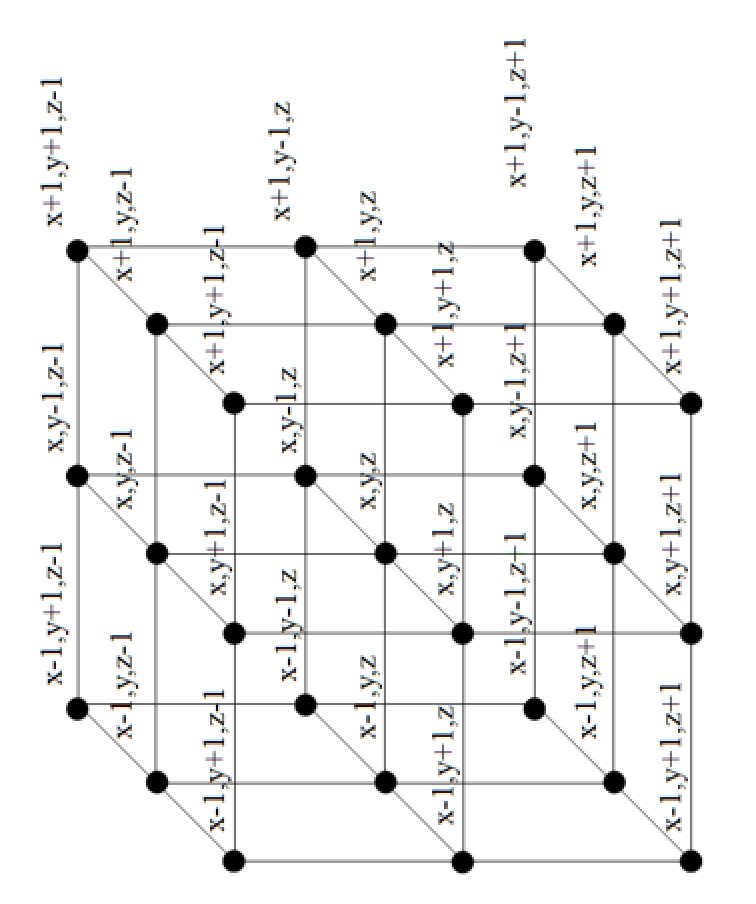
\includegraphics[angle=270,origin=b,width=0.65\textwidth]{resid.eps}
\caption{Resid}
\end{figure}

27����ư���������ƥ󥷥�׻��Ǥ��롥���٤ΥС����ȱ黻�ˤ��24��ʬ��׻�����
��RMGRP=24�ˡ����ƥ󥷥�׻��Ǥ����ΤΡ����٤�24��ʬ��׻����뤿�ᡤ
mapdist=0�Ǥ��롥

\begin{screen}
\tiny
\begin{verbatim}
resid( float *d, float *b, float *c )
     /*D3D[DP][HT][WD]*/
     /*B3D[DP][HT][WD]*/
     /*C3D[DP][HT][WD]*/
#define NCHIP     1
#define RMGRP     24
#define OMAP      1
#define PAD       1
#define RRANGE   ((HT-PAD*2)/NCHIP/OMAP)
  Ull  CHIP;
  Ull  LOOP1, LOOP0;
  Ull  INIT1, INIT0;
  Ull  AR[64][4];                     /* output of EX     in each unit */
  Ull  BR[64][4][4];                  /* output registers in each unit */
  Ull  r0, r1, r2, r3, r4, r5, r6, r7, r8, r9, r10, r11, r12, r13, r14, r15;
  Ull  r16, r17, r18, r19, r20, r21, r22, r23, r24, r25, r26, r27, r28, r29, r30, r31;
  Ull  cc0, cc1, cc2, cc3, ex0, ex1;
  int  x, y, z;
  int  row, col, n;
  Ull  roofs, coofs, bofs, cofs, dofs;
  union {float f; int i;} A0, A1, A2, A3;
  A0.f = -0.1;  A1.f = -0.2;  A2.f = -0.3;  A3.f = -0.4;
  Ull  I0 = A0.i;  Ull  I1 = A1.i;  Ull  I2 = A2.i;  Ull  I3 = A3.i;

#if !defined(EMAX5) && !defined(EMAX6)
  for (z=PAD; z<DP-PAD; z++) {
    for (y=PAD; y<HT-PAD; y++) {
      for (x=PAD; x<WD-PAD; x++) {
        *(d+z*WDHT+y*WD+x) = *(c+z*WDHT+y*WD+x)
                    + A0.f * *(b+(z  )*WDHT+(y  )*WD+x  )
                    + A1.f *(*(b+(z-1)*WDHT+(y  )*WD+x  )
                           + *(b+(z  )*WDHT+(y-1)*WD+x  )
                           + *(b+(z  )*WDHT+(y  )*WD+x-1)
                           + *(b+(z  )*WDHT+(y  )*WD+x+1)
                           + *(b+(z  )*WDHT+(y+1)*WD+x  )
                           + *(b+(z+1)*WDHT+(y  )*WD+x  ))
                    + A2.f *(*(b+(z-1)*WDHT+(y-1)*WD+x  )
                           + *(b+(z-1)*WDHT+(y  )*WD+x-1)
                           + *(b+(z-1)*WDHT+(y  )*WD+x+1)
                           + *(b+(z-1)*WDHT+(y+1)*WD+x  )
                           + *(b+(z  )*WDHT+(y-1)*WD+x-1)
                           + *(b+(z  )*WDHT+(y-1)*WD+x+1)
                           + *(b+(z  )*WDHT+(y+1)*WD+x-1)
                           + *(b+(z  )*WDHT+(y+1)*WD+x+1)
                           + *(b+(z+1)*WDHT+(y-1)*WD+x  )
                           + *(b+(z+1)*WDHT+(y  )*WD+x-1)
                           + *(b+(z+1)*WDHT+(y  )*WD+x+1)
                           + *(b+(z+1)*WDHT+(y+1)*WD+x  ))
                    + A3.f *(*(b+(z-1)*WDHT+(y-1)*WD+x-1)
                           + *(b+(z-1)*WDHT+(y-1)*WD+x+1)
                           + *(b+(z-1)*WDHT+(y+1)*WD+x-1)
                           + *(b+(z-1)*WDHT+(y+1)*WD+x+1)
                           + *(b+(z+1)*WDHT+(y-1)*WD+x-1)
                           + *(b+(z+1)*WDHT+(y-1)*WD+x+1)
                           + *(b+(z+1)*WDHT+(y+1)*WD+x-1)
                           + *(b+(z+1)*WDHT+(y+1)*WD+x+1));
  } } }
#endif
\end{verbatim}
\end{screen}

\begin{screen}
\tiny
\begin{verbatim}
  for (z=PAD; z<DP-PAD; z++) {
    for (y=0; y<RRANGE; y+=RMGRP) {
      Ull  btop[NCHIP], ctop[NCHIP], dtop[NCHIP];
      Ull  brow00[NCHIP], brow01[NCHIP], brow02[NCHIP], brow03[NCHIP], brow04[NCHIP], brow05[NCHIP], brow06[NCHIP], brow07[NCHIP], brow08[NCHIP];
      Ull  crow0[NCHIP];
      Ull  drow0[NCHIP];
      for (CHIP=0; CHIP<NCHIP; CHIP++) { /* output channels are parallelized by multi-chip (OC/#chip) */
        btop[CHIP]   = b               +(z  )*WDHT+(CHIP*RRANGE*OMAP+RRANGE*0+PAD+y  )*WD;
        ctop[CHIP]   = c               +(z  )*WDHT+(CHIP*RRANGE*OMAP+RRANGE*0+PAD+y  )*WD;
        dtop[CHIP]   = d               +(z  )*WDHT+(CHIP*RRANGE*OMAP+RRANGE*0+PAD+y  )*WD;
        brow00[CHIP] = b               +(z-1)*WDHT+(CHIP*RRANGE*OMAP+RRANGE*0+PAD+y-1)*WD;
        brow01[CHIP] = b               +(z-1)*WDHT+(CHIP*RRANGE*OMAP+RRANGE*0+PAD+y  )*WD;/* not used for RMGRP>1 */
        brow02[CHIP] = b               +(z-1)*WDHT+(CHIP*RRANGE*OMAP+RRANGE*0+PAD+y+1)*WD;/* not used for RMGRP>1 */
        brow03[CHIP] = b               +(z  )*WDHT+(CHIP*RRANGE*OMAP+RRANGE*0+PAD+y-1)*WD;
        brow04[CHIP] = b               +(z  )*WDHT+(CHIP*RRANGE*OMAP+RRANGE*0+PAD+y  )*WD;/* not used for RMGRP>1 */
        brow05[CHIP] = b               +(z  )*WDHT+(CHIP*RRANGE*OMAP+RRANGE*0+PAD+y+1)*WD;/* not used for RMGRP>1 */
        brow06[CHIP] = b               +(z+1)*WDHT+(CHIP*RRANGE*OMAP+RRANGE*0+PAD+y-1)*WD;
        brow07[CHIP] = b               +(z+1)*WDHT+(CHIP*RRANGE*OMAP+RRANGE*0+PAD+y  )*WD;/* not used for RMGRP>1 */
        brow08[CHIP] = b               +(z+1)*WDHT+(CHIP*RRANGE*OMAP+RRANGE*0+PAD+y+1)*WD;/* not used for RMGRP>1 */
        crow0[CHIP]  = c               +(z  )*WDHT+(CHIP*RRANGE*OMAP+RRANGE*0+PAD+y  )*WD;
        drow0[CHIP]  = d               +(z  )*WDHT+(CHIP*RRANGE*OMAP+RRANGE*0+PAD+y  )*WD;
      }
//EMAX5A begin resid mapdist=0 /* 12 */
      for (CHIP=0; CHIP<NCHIP; CHIP++) { /* output channels are parallelized by multi-chip (OC/#chip) */
   /*2*/for (INIT1=1,LOOP1=RMGRP,roofs=0-WD*4; LOOP1--; INIT1=0) {      /* stage#0 *//* mapped to FOR() on BR[63][1][0] */
     /*1*/for (INIT0=1,LOOP0=WD-PAD*2,coofs=(PAD-1)*4; LOOP0--; INIT0=0) {          /* stage#0 *//* mapped to FOR() on BR[63][0][0] */
            exe(OP_ADD,  &coofs, INIT0?coofs:coofs, EXP_H3210, 4, EXP_H3210, 0LL, EXP_H3210, OP_AND, 0x00000000ffffffffLL, OP_NOP, 0LL); /* stage#0 */
            exe(OP_ADD,  &roofs, roofs,  EXP_H3210, INIT0?WD*4:0, EXP_H3210, 0LL, EXP_H3210, OP_AND, 0x00000000ffffffffLL, OP_NOP, 0LL); /* stage#0 */
            exe(OP_ADD3, &bofs,  btop[CHIP], EXP_H3210, roofs, EXP_H3210,  coofs, EXP_H3210, OP_AND, 0x000000ffffffffffLL, OP_NOP, 0LL); /* stage#1 */
            exe(OP_ADD3, &cofs,  ctop[CHIP], EXP_H3210, roofs, EXP_H3210,  coofs, EXP_H3210, OP_AND, 0x000000ffffffffffLL, OP_NOP, 0LL); /* stage#1 */
            exe(OP_ADD3, &dofs,  dtop[CHIP], EXP_H3210, roofs, EXP_H3210,  coofs, EXP_H3210, OP_AND, 0x000000ffffffffffLL, OP_NOP, 0LL); /* stage#1 */
            /*map0*/
            mop(OP_LDWR, 1, &BR[2][0][1], bofs, (0       -WDHT-WD-1)*4, MSK_D0, brow00[CHIP], WD*(RMGRP+PAD*2), 0, 0, NULL, WD*(RMGRP+PAD*2));/* stage#2 */
            mop(OP_LDWR, 1, &BR[2][0][0], bofs, (0       -WDHT-WD  )*4, MSK_D0, brow00[CHIP], WD*(RMGRP+PAD*2), 0, 0, NULL, WD*(RMGRP+PAD*2));/* stage#2 */
            mop(OP_LDWR, 1, &BR[2][1][1], bofs, (0       -WDHT-WD+1)*4, MSK_D0, brow00[CHIP], WD*(RMGRP+PAD*2), 0, 0, NULL, WD*(RMGRP+PAD*2));/* stage#2 */
            exe(OP_FML, &r0, BR[2][0][1], EXP_H3210,  I3,          EXP_H3210,  0,           EXP_H3210, OP_NOP, 0LL, OP_NOP, 0LL);      /* stage#3 */
            exe(OP_FML, &r1, BR[2][0][0], EXP_H3210,  I2,          EXP_H3210,  0,           EXP_H3210, OP_NOP, 0LL, OP_NOP, 0LL);      /* stage#3 */
            exe(OP_FML, &r2, BR[2][1][1], EXP_H3210,  I3,          EXP_H3210,  0,           EXP_H3210, OP_NOP, 0LL, OP_NOP, 0LL);      /* stage#3 */
            mop(OP_LDWR, 1, &BR[3][0][1], bofs, (0       -WDHT   -1)*4, MSK_D0, brow00[CHIP], WD*(RMGRP+PAD*2), 0, 0, NULL, WD*(RMGRP+PAD*2));/* stage#3 */
            mop(OP_LDWR, 1, &BR[3][0][0], bofs, (0       -WDHT     )*4, MSK_D0, brow00[CHIP], WD*(RMGRP+PAD*2), 0, 0, NULL, WD*(RMGRP+PAD*2));/* stage#3 */
            mop(OP_LDWR, 1, &BR[3][1][1], bofs, (0       -WDHT   +1)*4, MSK_D0, brow00[CHIP], WD*(RMGRP+PAD*2), 0, 0, NULL, WD*(RMGRP+PAD*2));/* stage#3 */
            exe(OP_FMA, &r3, r0,          EXP_H3210,  BR[3][0][1], EXP_H3210,  I2,          EXP_H3210, OP_NOP, 0LL, OP_NOP, 0LL);      /* stage#4 */
            exe(OP_FMA, &r4, r1,          EXP_H3210,  BR[3][0][0], EXP_H3210,  I1,          EXP_H3210, OP_NOP, 0LL, OP_NOP, 0LL);      /* stage#4 */
            exe(OP_FMA, &r5, r2,          EXP_H3210,  BR[3][1][1], EXP_H3210,  I2,          EXP_H3210, OP_NOP, 0LL, OP_NOP, 0LL);      /* stage#4 */
            mop(OP_LDWR, 1, &BR[4][0][1], bofs, (0       -WDHT+WD-1)*4, MSK_D0, brow00[CHIP], WD*(RMGRP+PAD*2), 0, 0, NULL, WD*(RMGRP+PAD*2));/* stage#4 */
            mop(OP_LDWR, 1, &BR[4][0][0], bofs, (0       -WDHT+WD  )*4, MSK_D0, brow00[CHIP], WD*(RMGRP+PAD*2), 0, 0, NULL, WD*(RMGRP+PAD*2));/* stage#4 */
            mop(OP_LDWR, 1, &BR[4][1][1], bofs, (0       -WDHT+WD+1)*4, MSK_D0, brow00[CHIP], WD*(RMGRP+PAD*2), 0, 0, NULL, WD*(RMGRP+PAD*2));/* stage#4 */
            exe(OP_FMA, &r6, r3,          EXP_H3210,  BR[4][0][1], EXP_H3210,  I3,          EXP_H3210, OP_NOP, 0LL, OP_NOP, 0LL);      /* stage#5 */
            exe(OP_FMA, &r7, r4,          EXP_H3210,  BR[4][0][0], EXP_H3210,  I2,          EXP_H3210, OP_NOP, 0LL, OP_NOP, 0LL);      /* stage#5 */
            exe(OP_FMA, &r8, r5,          EXP_H3210,  BR[4][1][1], EXP_H3210,  I3,          EXP_H3210, OP_NOP, 0LL, OP_NOP, 0LL);      /* stage#5 */

            mop(OP_LDWR, 1, &BR[5][0][1], bofs, (0            -WD-1)*4, MSK_D0, brow03[CHIP], WD*(RMGRP+PAD*2), 0, 0, NULL, WD*(RMGRP+PAD*2));/* stage#5 */
            mop(OP_LDWR, 1, &BR[5][0][0], bofs, (0            -WD  )*4, MSK_D0, brow03[CHIP], WD*(RMGRP+PAD*2), 0, 0, NULL, WD*(RMGRP+PAD*2));/* stage#5 */
            mop(OP_LDWR, 1, &BR[5][1][1], bofs, (0            -WD+1)*4, MSK_D0, brow03[CHIP], WD*(RMGRP+PAD*2), 0, 0, NULL, WD*(RMGRP+PAD*2));/* stage#5 */
            exe(OP_FMA, &r0, r6,          EXP_H3210,  BR[5][0][1], EXP_H3210,  I2,          EXP_H3210, OP_NOP, 0LL, OP_NOP, 0LL);      /* stage#6 */
            exe(OP_FMA, &r1, r7,          EXP_H3210,  BR[5][0][0], EXP_H3210,  I1,          EXP_H3210, OP_NOP, 0LL, OP_NOP, 0LL);      /* stage#6 */
            exe(OP_FMA, &r2, r8,          EXP_H3210,  BR[5][1][1], EXP_H3210,  I2,          EXP_H3210, OP_NOP, 0LL, OP_NOP, 0LL);      /* stage#6 */
            mop(OP_LDWR, 1, &BR[6][0][1], bofs, (0               -1)*4, MSK_D0, brow03[CHIP], WD*(RMGRP+PAD*2), 0, 0, NULL, WD*(RMGRP+PAD*2));/* stage#6 */
            mop(OP_LDWR, 1, &BR[6][0][0], bofs, (0                 )*4, MSK_D0, brow03[CHIP], WD*(RMGRP+PAD*2), 0, 0, NULL, WD*(RMGRP+PAD*2));/* stage#6 */
            mop(OP_LDWR, 1, &BR[6][1][1], bofs, (0               +1)*4, MSK_D0, brow03[CHIP], WD*(RMGRP+PAD*2), 0, 0, NULL, WD*(RMGRP+PAD*2));/* stage#6 */
            exe(OP_FMA, &r3, r0,          EXP_H3210,  BR[6][0][1], EXP_H3210,  I1,          EXP_H3210, OP_NOP, 0LL, OP_NOP, 0LL);      /* stage#7 */
            exe(OP_FMA, &r4, r1,          EXP_H3210,  BR[6][0][0], EXP_H3210,  I0,          EXP_H3210, OP_NOP, 0LL, OP_NOP, 0LL);      /* stage#7 */
            exe(OP_FMA, &r5, r2,          EXP_H3210,  BR[6][1][1], EXP_H3210,  I1,          EXP_H3210, OP_NOP, 0LL, OP_NOP, 0LL);      /* stage#7 */
            mop(OP_LDWR, 1, &BR[7][0][1], bofs, (0            +WD-1)*4, MSK_D0, brow03[CHIP], WD*(RMGRP+PAD*2), 0, 0, NULL, WD*(RMGRP+PAD*2));/* stage#7 */
            mop(OP_LDWR, 1, &BR[7][0][0], bofs, (0            +WD  )*4, MSK_D0, brow03[CHIP], WD*(RMGRP+PAD*2), 0, 0, NULL, WD*(RMGRP+PAD*2));/* stage#7 */
            mop(OP_LDWR, 1, &BR[7][1][1], bofs, (0            +WD+1)*4, MSK_D0, brow03[CHIP], WD*(RMGRP+PAD*2), 0, 0, NULL, WD*(RMGRP+PAD*2));/* stage#7 */
            exe(OP_FMA, &r6, r3,          EXP_H3210,  BR[7][0][1], EXP_H3210,  I2,          EXP_H3210, OP_NOP, 0LL, OP_NOP, 0LL);      /* stage#8 */
            exe(OP_FMA, &r7, r4,          EXP_H3210,  BR[7][0][0], EXP_H3210,  I1,          EXP_H3210, OP_NOP, 0LL, OP_NOP, 0LL);      /* stage#8 */
            exe(OP_FMA, &r8, r5,          EXP_H3210,  BR[7][1][1], EXP_H3210,  I2,          EXP_H3210, OP_NOP, 0LL, OP_NOP, 0LL);      /* stage#8 */

            mop(OP_LDWR, 1, &BR[8][0][1], bofs, (0       +WDHT-WD-1)*4, MSK_D0, brow06[CHIP], WD*(RMGRP+PAD*2), 0, 0, NULL, WD*(RMGRP+PAD*2));/* stage#8 */
            mop(OP_LDWR, 1, &BR[8][0][0], bofs, (0       +WDHT-WD  )*4, MSK_D0, brow06[CHIP], WD*(RMGRP+PAD*2), 0, 0, NULL, WD*(RMGRP+PAD*2));/* stage#8 */
            mop(OP_LDWR, 1, &BR[8][1][1], bofs, (0       +WDHT-WD+1)*4, MSK_D0, brow06[CHIP], WD*(RMGRP+PAD*2), 0, 0, NULL, WD*(RMGRP+PAD*2));/* stage#8 */
            exe(OP_FMA, &r0, r6,          EXP_H3210,  BR[8][0][1], EXP_H3210,  I3,          EXP_H3210, OP_NOP, 0LL, OP_NOP, 0LL);      /* stage#9 */
            exe(OP_FMA, &r1, r7,          EXP_H3210,  BR[8][0][0], EXP_H3210,  I2,          EXP_H3210, OP_NOP, 0LL, OP_NOP, 0LL);      /* stage#9 */
            exe(OP_FMA, &r2, r8,          EXP_H3210,  BR[8][1][1], EXP_H3210,  I3,          EXP_H3210, OP_NOP, 0LL, OP_NOP, 0LL);      /* stage#9 */
            mop(OP_LDWR, 1, &BR[9][0][1], bofs, (0       +WDHT   -1)*4, MSK_D0, brow06[CHIP], WD*(RMGRP+PAD*2), 0, 0, NULL, WD*(RMGRP+PAD*2));/* stage#9 */
            mop(OP_LDWR, 1, &BR[9][0][0], bofs, (0       +WDHT     )*4, MSK_D0, brow06[CHIP], WD*(RMGRP+PAD*2), 0, 0, NULL, WD*(RMGRP+PAD*2));/* stage#9 */
            mop(OP_LDWR, 1, &BR[9][1][1], bofs, (0       +WDHT   +1)*4, MSK_D0, brow06[CHIP], WD*(RMGRP+PAD*2), 0, 0, NULL, WD*(RMGRP+PAD*2));/* stage#9 */
            exe(OP_FMA, &r3, r0,          EXP_H3210,  BR[9][0][1], EXP_H3210,  I2,          EXP_H3210, OP_NOP, 0LL, OP_NOP, 0LL);      /* stage#10*/
            exe(OP_FMA, &r4, r1,          EXP_H3210,  BR[9][0][0], EXP_H3210,  I1,          EXP_H3210, OP_NOP, 0LL, OP_NOP, 0LL);      /* stage#10*/
            exe(OP_FMA, &r5, r2,          EXP_H3210,  BR[9][1][1], EXP_H3210,  I2,          EXP_H3210, OP_NOP, 0LL, OP_NOP, 0LL);      /* stage#10*/
            mop(OP_LDWR, 1, &BR[10][0][1],bofs, (0       +WDHT+WD-1)*4, MSK_D0, brow06[CHIP], WD*(RMGRP+PAD*2), 0, 0, NULL, WD*(RMGRP+PAD*2));/* stage#10*/
            mop(OP_LDWR, 1, &BR[10][0][0],bofs, (0       +WDHT+WD  )*4, MSK_D0, brow06[CHIP], WD*(RMGRP+PAD*2), 0, 0, NULL, WD*(RMGRP+PAD*2));/* stage#10*/
            mop(OP_LDWR, 1, &BR[10][1][1],bofs, (0       +WDHT+WD+1)*4, MSK_D0, brow06[CHIP], WD*(RMGRP+PAD*2), 0, 0, NULL, WD*(RMGRP+PAD*2));/* stage#10*/
            exe(OP_FMA, &r6, r3,          EXP_H3210,  BR[10][0][1],EXP_H3210,  I3,          EXP_H3210, OP_NOP, 0LL, OP_NOP, 0LL);      /* stage#11*/
            exe(OP_FMA, &r7, r4,          EXP_H3210,  BR[10][0][0],EXP_H3210,  I2,          EXP_H3210, OP_NOP, 0LL, OP_NOP, 0LL);      /* stage#11*/
            exe(OP_FMA, &r8, r5,          EXP_H3210,  BR[10][1][1],EXP_H3210,  I3,          EXP_H3210, OP_NOP, 0LL, OP_NOP, 0LL);      /* stage#11*/
            mop(OP_LDWR, 1, &BR[11][0][1],cofs, (0                 )*4, MSK_D0, crow0[CHIP],  WD*RMGRP, 0, 0, NULL, WD*RMGRP);     /* stage#11*/
            exe(OP_FAD, &r1, r6,          EXP_H3210,  BR[11][0][1],EXP_H3210,  0,           EXP_H3210, OP_NOP, 0LL, OP_NOP, 0LL);      /* stage#12*/
            exe(OP_FAD, &r2, r7,          EXP_H3210,  r8,          EXP_H3210,  0,           EXP_H3210, OP_NOP, 0LL, OP_NOP, 0LL);      /* stage#12*/
            exe(OP_FAD, &r0, r1,          EXP_H3210,  r2,          EXP_H3210,  0,           EXP_H3210, OP_NOP, 0LL, OP_NOP, 0LL);      /* stage#13*/
            mop(OP_STWR, 3, &r0,          dofs, (0                 )*4, MSK_D0, drow0[CHIP],  WD*RMGRP, 0, 0, NULL, WD*RMGRP);     /* stage#13*/
          }
        }
      }
//EMAX5A end
    }
//EMAX5A drain_dirty_lmm
  }
\end{verbatim}
\end{screen}

\begin{figure}[htbp]
\center
\epsfile{file=stencil+rmm-resid-emax6.eps,width=1.00\textwidth}
\caption{Resid}
\end{figure}

\clearpage

\subsection{Wave2d with stencil}

\begin{figure}[htbp]
\center
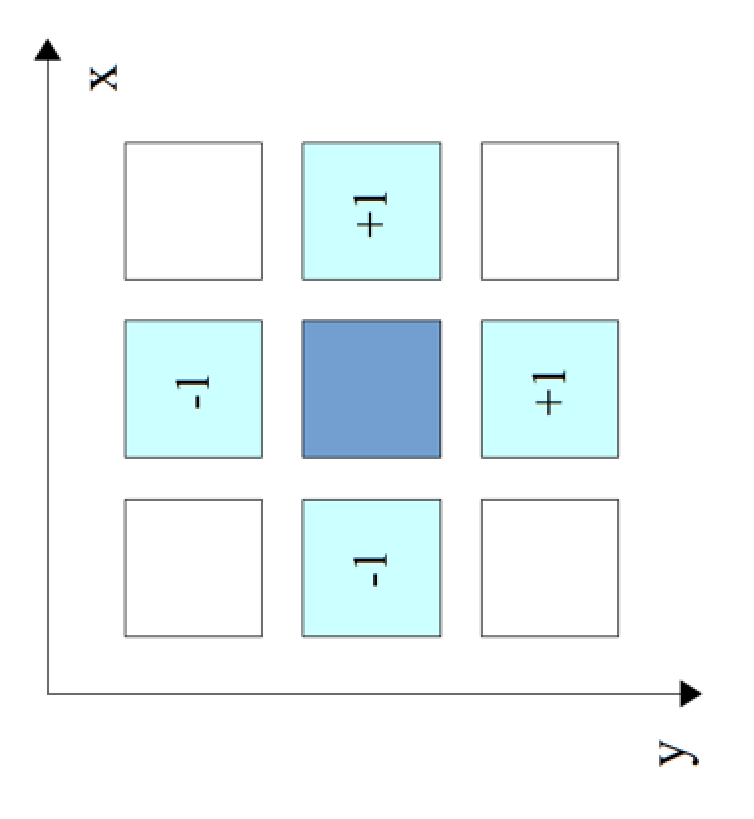
\includegraphics[angle=270,origin=b,width=0.60\textwidth]{wave2d.eps}
\caption{Wave2d}
\end{figure}

5����ư���������ƥ󥷥�׻��Ǥ��롥���٤ΥС����ȱ黻�ˤ��24��ʬ��׻�����
��RMGRP=24�ˡ����ƥ󥷥�׻��Ǥ����ΤΡ����٤�24��ʬ��׻����뤿�ᡤ
mapdist=0�Ǥ��롥�ʤ���̤����stage����Ѥ���PLOAD�ˤ����ǽ���夬��ǽ�Ǥ��롥
��������PAD>1�ξ�硤LOAD�о�LMM��PLOAD�о�LMM���ΰ褬������ʣ���뤿�ᡤ
PLOAD����AXI�ȥ�󥶥������LOAD�о�LMM�ˤ�ҥåȤ��롥load��������ˤ���
��AXI���Ԥ����졤AXI�����ڤ��뤳�Ȥ����롥

\begin{screen}
\tiny
\begin{verbatim}
wave2d( float *z2, float *z0, float *z1 )
     /*WZ2[HT][WD]*/
     /*WZ0[HT][WD]*/
     /*WZ1[HT][WD]*/
#define NCHIP     1
#define RMGRP     24
#define OMAP      1
#define PAD       1
#define RRANGE   ((HT-PAD*2)/NCHIP/OMAP)
  Ull  CHIP;
  Ull  LOOP1, LOOP0;
  Ull  INIT1, INIT0;
  Ull  AR[64][4];                     /* output of EX     in each unit */
  Ull  BR[64][4][4];                  /* output registers in each unit */
  Ull  r0, r1, r2, r3, r4, r5, r6, r7, r8, r9, r10, r11, r12, r13, r14, r15;
  Ull  r16, r17, r18, r19, r20, r21, r22, r23, r24, r25, r26, r27, r28, r29, r30, r31;
  Ull  cc0, cc1, cc2, cc3, ex0, ex1;
  int  x, y, z;
  int  row, col, n;
  Ull  roofs, coofs, z0ofs, z1ofs, z2ofs;
  union {float f; int i;} C1, C2, C3, C4;
  C1.f =  2.00;
  C2.f = -1.00;
  C3.f =  0.25;
  C4.f = -4.00;
  Ull  I1 = C1.i;
  Ull  I2 = C2.i;
  Ull  I3 = C3.i;
  Ull  I4 = C4.i;

#if !defined(EMAX5) && !defined(EMAX6)
  for (y=PAD; y<HT-PAD; y++) {
    for (x=PAD; x<WD-PAD; x++) {
      *(z2+y*WD+x) =  C1.f * *(z1+y*WD+x)
                   +  C2.f * *(z0+y*WD+x)
                   +  C3.f *(*(z1+(y+1)*WD+x  )
                           + *(z1+(y-1)*WD+x  )
                           + *(z1+(y  )*WD+x-1)
                           + *(z1+(y  )*WD+x+1) + C4.f * *(z1+y*WD+x));
    }
  }
#endif
\end{verbatim}
\end{screen}

\begin{screen}
\tiny
\begin{verbatim}
  for (y=0; y<RRANGE; y+=RMGRP) {
    Ull  z0top[NCHIP], z1top[NCHIP], z2top[NCHIP];
    Ull  z0row0[NCHIP];
    Ull  z1row00[NCHIP], z1row01[NCHIP], z1row02[NCHIP];
    Ull  z2row0[NCHIP];
    for (CHIP=0; CHIP<NCHIP; CHIP++) { /* output channels are parallelized by multi-chip (OC/#chip) */
      z0top[CHIP]   = z0              +(CHIP*RRANGE*OMAP+RRANGE*0+PAD+y  )*WD;
      z1top[CHIP]   = z1              +(CHIP*RRANGE*OMAP+RRANGE*0+PAD+y  )*WD;
      z2top[CHIP]   = z2              +(CHIP*RRANGE*OMAP+RRANGE*0+PAD+y  )*WD;
      z0row0[CHIP]  = z0              +(CHIP*RRANGE*OMAP+RRANGE*0+PAD+y  )*WD;
      z1row00[CHIP] = z1              +(CHIP*RRANGE*OMAP+RRANGE*0+PAD+y-1)*WD;
      z1row01[CHIP] = z1              +(CHIP*RRANGE*OMAP+RRANGE*0+PAD+y  )*WD;/* not used for RMGRP>1 */
      z1row02[CHIP] = z1              +(CHIP*RRANGE*OMAP+RRANGE*0+PAD+y+1)*WD;/* not used for RMGRP>1 */
      z2row0[CHIP]  = z2              +(CHIP*RRANGE*OMAP+RRANGE*0+PAD+y  )*WD;
    }
//EMAX5A begin wave2d mapdist=0 /* 8 */
    for (CHIP=0; CHIP<NCHIP; CHIP++) { /* output channels are parallelized by multi-chip (OC/#chip) */
 /*2*/for (INIT1=1,LOOP1=RMGRP,roofs=0-WD*4; LOOP1--; INIT1=0) {      /* stage#0 *//* mapped to FOR() on BR[63][1][0] */
   /*1*/for (INIT0=1,LOOP0=WD-PAD*2,coofs=(PAD-1)*4; LOOP0--; INIT0=0) {          /* stage#0 *//* mapped to FOR() on BR[63][0][0] */
          exe(OP_ADD,  &coofs, INIT0?coofs:coofs, EXP_H3210, 4, EXP_H3210,  0LL, EXP_H3210, OP_AND, 0x00000000ffffffffLL, OP_NOP, 0LL); /* stage#0 */
          exe(OP_ADD,  &roofs, roofs,  EXP_H3210, INIT0?WD*4:0, EXP_H3210,  0LL, EXP_H3210, OP_AND, 0x00000000ffffffffLL, OP_NOP, 0LL); /* stage#0 */
          exe(OP_ADD3, &z0ofs, z0top[CHIP], EXP_H3210, roofs, EXP_H3210,  coofs, EXP_H3210, OP_AND, 0x000000ffffffffffLL, OP_NOP, 0LL); /* stage#1 */
          exe(OP_ADD3, &z1ofs, z1top[CHIP], EXP_H3210, roofs, EXP_H3210,  coofs, EXP_H3210, OP_AND, 0x000000ffffffffffLL, OP_NOP, 0LL); /* stage#1 */
          exe(OP_ADD3, &z2ofs, z2top[CHIP], EXP_H3210, roofs, EXP_H3210,  coofs, EXP_H3210, OP_AND, 0x000000ffffffffffLL, OP_NOP, 0LL); /* stage#1 */
          /*map0*/
          mop(OP_LDWR, 1, &BR[2][0][1], z0ofs, (0                  )*4, MSK_D0, z0row0[CHIP],  WD*RMGRP, 0, 0, NULL, WD*RMGRP);  /* stage#2 */
          exe(OP_FML, &r0, BR[2][0][1], EXP_H3210,  I2,          EXP_H3210,  0,           EXP_H3210, OP_NOP, 0LL, OP_NOP, 0LL);      /* stage#3 */
          mop(OP_LDWR, 1, &BR[3][0][1], z1ofs, (0             -WD  )*4, MSK_D0, z1row00[CHIP], WD*(RMGRP+PAD*2), 0, 0, NULL, WD*(RMGRP+PAD*2)); /* stage#3 */
          mop(OP_LDWR, 1, &BR[4][0][1], z1ofs, (0                -1)*4, MSK_D0, z1row00[CHIP], WD*(RMGRP+PAD*2), 0, 0, NULL, WD*(RMGRP+PAD*2)); /* stage#4 */
          mop(OP_LDWR, 1, &BR[4][0][0], z1ofs, (0                  )*4, MSK_D0, z1row00[CHIP], WD*(RMGRP+PAD*2), 0, 0, NULL, WD*(RMGRP+PAD*2)); /* stage#4 */
          mop(OP_LDWR, 1, &BR[4][1][1], z1ofs, (0                +1)*4, MSK_D0, z1row00[CHIP], WD*(RMGRP+PAD*2), 0, 0, NULL, WD*(RMGRP+PAD*2)); /* stage#4 */
          exe(OP_FAD, &r1, BR[3][0][1], EXP_H3210,  BR[4][0][1], EXP_H3210,  0,           EXP_H3210, OP_NOP, 0LL, OP_NOP, 0LL);      /* stage#5 */
          mop(OP_LDWR, 1, &BR[5][0][1], z1ofs, (0             +WD  )*4, MSK_D0, z1row00[CHIP], WD*(RMGRP+PAD*2), 0, 0, NULL, WD*(RMGRP+PAD*2)); /* stage#5 */
          exe(OP_FMA, &r2, r1,          EXP_H3210,  BR[4][0][0], EXP_H3210,  I4,          EXP_H3210, OP_NOP, 0LL, OP_NOP, 0LL);      /* stage#6 */
          exe(OP_FAD, &r3, BR[4][1][1], EXP_H3210,  BR[5][0][1], EXP_H3210,  0,           EXP_H3210, OP_NOP, 0LL, OP_NOP, 0LL);      /* stage#6 */
          exe(OP_FAD, &r4, r2,          EXP_H3210,  r3,          EXP_H3210,  0,           EXP_H3210, OP_NOP, 0LL, OP_NOP, 0LL);      /* stage#7 */
          exe(OP_FMA, &r5, r0,          EXP_H3210,  r4,          EXP_H3210,  I3,          EXP_H3210, OP_NOP, 0LL, OP_NOP, 0LL);      /* stage#8 */
          exe(OP_FMA, &r6, r5,          EXP_H3210,  BR[4][0][0], EXP_H3210,  I1,          EXP_H3210, OP_NOP, 0LL, OP_NOP, 0LL);      /* stage#9 */
          mop(OP_STWR, 3, &r6,          z2ofs, (0                  )*4, MSK_D0, z2row0[CHIP],  WD*RMGRP, 0, 0, NULL, WD*RMGRP);  /* stage#9 */
        }
      }
    }
//EMAX5A end
  }
//EMAX5A drain_dirty_lmm
\end{verbatim}
\end{screen}

\begin{figure}[htbp]
\center
\epsfile{file=stencil+rmm-wave2d-emax6.eps,width=1.00\textwidth}
\caption{Wave2d}
\end{figure}

\clearpage

\section{���ѥ����ͥ�}

\subsection{3x3���߹���}

\shabox{
\leftline{cent\% make -f Makefile-csim.emax6+dma cnn-csim.emax6+dma clean}
\leftline{cent\% ../../src/csim/csim -x cnn-csim.emax6+dma}
}

\shabox{
\leftline{zynq\% make -f Makefile-zynq.emax6+dma cnn-zynq.emax6+dma clean}
\leftline{zynq\% ./cnn-zynq.emax6+dma}
}

\begin{figure}[htbp]
\center
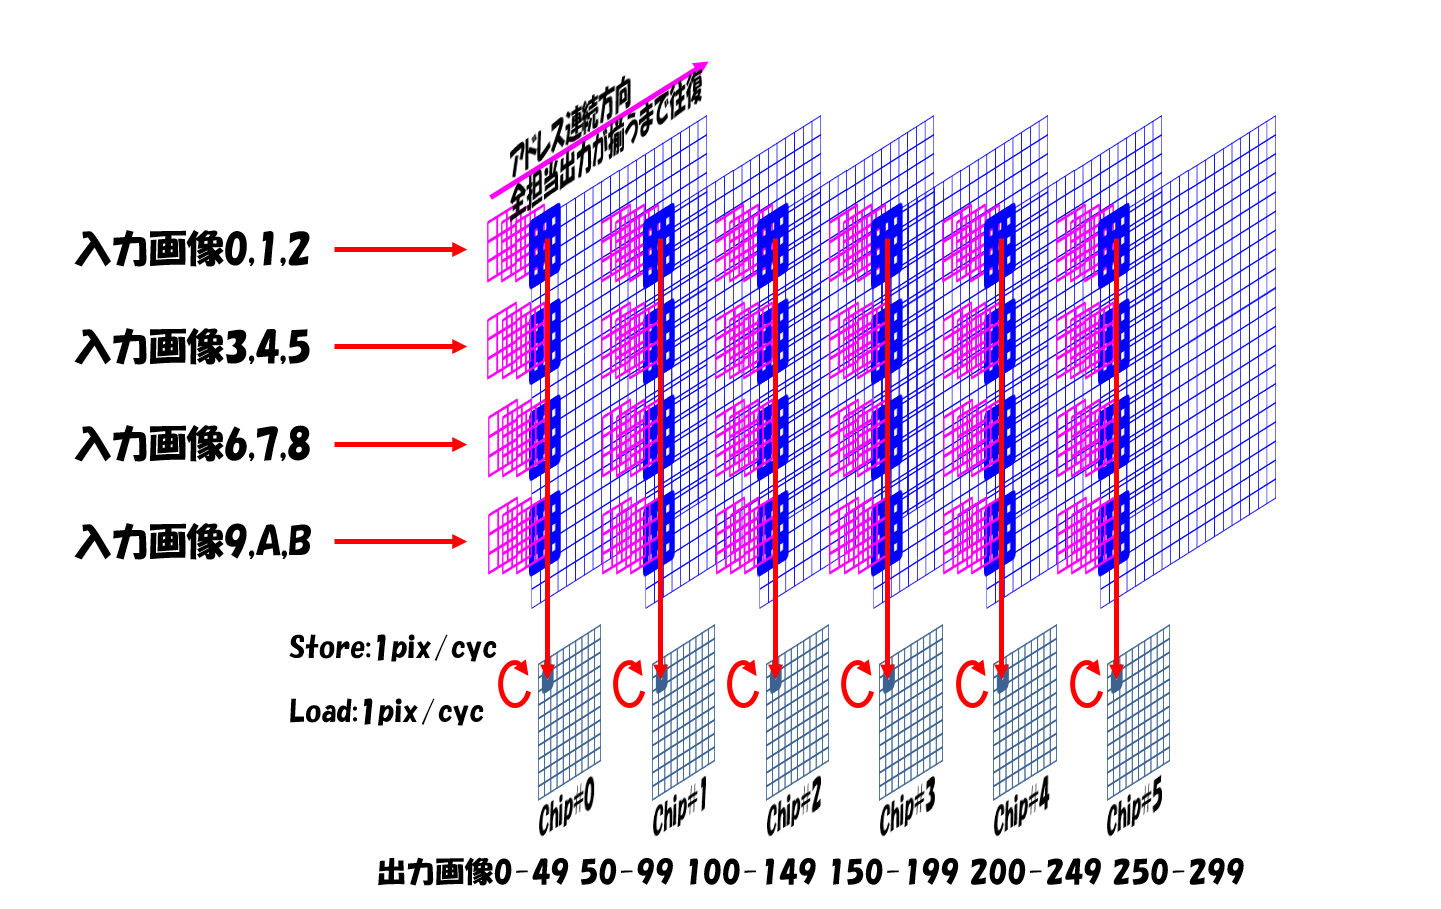
\includegraphics[angle=270,origin=b,width=0.65\textwidth]{EMAX6CNN.eps}
\caption{\label{cnn}CNN���}
\end{figure}

��\ref{cnn}�ϡ����ѥץ�������1�ĤǤ���Alexnet�ξ��߹��߱黻��CNN�ˤˤ�����
�ǡ�����ή��Ǥ��롥���ϲ����ΰ����ȥ����ͥ�ʽŤߡˤ����±黻��̤��ᡤʣ
�����ϲ��������˲û�������Τ���ϲ����ΰ����Ȥ���ʣ��Ĥν��ϲ��������뤿��
�������ϲ�����ɬ�סˡ������ϲ����β��ǿ��Ͻ����˸�������������ä��롥���ϲ�
���ϼ��ν��������ϲ����Ȥʤ뤿�ᡤ������ϲ����������ϲ�������Ǥ��롥����
����ϡ��ɥ���������ݻ��Ǥ��ʤ�����Ǥϡ����ϲ����Ͻ缡�֥����ɥ��㥹�Ȥ���
���ϲ���ñ�̤˱黻��ʬ�䤷�����ϲ����˼��ν����ͤ��߻��Ǥ���ϡ��ɥ���������
��Ŭ���Ƥ��롥

\begin{figure}[htbp]
\center

\includegraphics[width=0.90\textwidth]{cnn0.eps}
\caption{\label{fig:cnn0}Cnn}
\end{figure}

242x242�ξ��߹��߱黻�Ǥ��롥���٤ΥС����ȱ黻�ˤ��8��ʬ��׻�����
��RMGRP=8�ˡ����ƥ󥷥�׻��Ǥ����ΤΡ����٤�8��ʬ��׻����뤿�ᡤ
mapdist=0�Ǥ��롥��\ref{fig:cnn0}(a)�ˡ�CNN�Υǡ�����¤��(b)�˳�unit�����±�
�����1��������(K$^2$+1)xW������CGRA�򼨤���M$\ge$K, OC$\ge$W����ˡ�(b)��
��ñ�Τ���ˡ�Ʊ�����Υ��ʥåץ���åȤǤϤʤ����ǡ����ե�������դ򼨤���
���롥�ºݤΥϡ��ɥ������ǤϿ�\ref{fig:mm0}(c)�Τ褦�˳��ʤΥǡ������ѥ��ץ�
�����������롥CNN�ϡ�����in�ΰ�����KxK�ˤ�kernel��KxK�ˤ����·�̤�������
����ͥ�ʬ�߻���������out�˳�Ǽ���롥���Ϥ�����ɿ���M$^2$xIC��kernel����
��ɿ��ϡ�K$^2$�����ϥ���ͥ����IC�ˤȽ��ϥ���ͥ����OC�ˤ�褸��
K$^2$xICxOC�����Ϥ�����ɿ���M$^2$xOC�Ȥʤ롥CNN���Ѥ�����K�ϴ���Ǥ��ꡤ
������Ŭ����ϡ��ɥ������ѥ�᥿W���б�������ȱ黻���ƯΨ���㲼���롥KxK��
���±黻��1���unit[*][oc mod W]���б������ƥѥ��ץ饤��¹Ԥ���W�Ĥν��ϥ���
�ͥ��Ʊ���˷׻������K$^2$xW�����黻������ѤǤ���Ψ���褤�ʤ�����K�ʤ�LMM
���Ф���֥����ɥ��㥹�ȵ�ǽ��ɬ�סˡ�(c)�Ϥ���ˡ�OC��N���åפ�ʬ�䤷������
���������ƥ��åפ�K$^2$�ʤ����±黻��REP��xW������Ǥ����ʿ�������������˳�
LMM����in��1�ԡ�M���ǡ�x GRP��ʬ�ȡ���kernel��IC*OC*K*K���ǡˤ���ƤǤ����
��μ����Ǥ��롥������7�ť롼�פ������åפ�CGRA��1��ư����������б�����
chip�롼�פγƥ����졼����󤬡��ƥ��åפˤ�����REP�Ȥ����ϥ���ͥ��kernel
�Ȥξ��߹��߱黻�ˤ��W�Ȥν��ϥ���ͥ��GRP��ʬ�׻�����������б����롥��¦
�롼�פ�oc��0����OC/N-1�ޤ����ä���֡��ƥ��åפκǽ��ʤ����LMM��in��GRP��
ʬ�ݻ����롥�������ǽ��ʤ�LMM��oc�򹹿������٤������ؤ���ɬ�פ����롥�ʾ��
�黻���פ�������Ū����������ϡ�CGRA��ư�����ٱ��K$^2$xREP��������ˤ����
LMM�����촹�����֤������K$^2$x(M-2)$^2$xICxOC/(K$^2$xREPxWxN) =
(M-2)$^2$xICxOC/(REPxWxN)�Ȥʤ롥�ޤ���LMM��in��kernel��out���Τ���ƤǤ���
��������ŪDDR-LMM��ž���̤�M$^2$xIC + K$^2$xICxOC + M$^2$xOC�Ǥ���Τ��Ф���
��LMM��in��MxGRP��out��MxGRPxW��kernel�Τ��������ƤǤ������ž���̤ϡ�in��
kernel���ơ�M$^2$xIC��K$^2$xICxOC��out��1��ʬ�����촹���̤�(MxGRPxW)x2�����
���β�ž��(OC/N/W)x(IC/REP)x(M/GRP)��N��褸������������ؤ���ȯ�����뤿��
M$^2$x2xOCxIC/REP��IC=REP�ξ��out�ϰ��٤Ƿ׻��Ǥ����촹�����פΤ���DDR����
�Τߤ�M$^2$xOC��N�����¸�ˤȤʤ롥

\begin{screen}
\tiny
\begin{verbatim}
orig() {
  for (ic=0; ic<IC; ic++) { /* set input channel */
    ip0 = &in[ic*M*M]; /* top of input */
    for (row=1; row<M-1; row++) { /* image loop */
      for (col=1; col<M-1; col++) {
        for (oc=0; oc<OC; oc++) { /* set output channel */
          op = &out0[oc*M*M+row*M+col]; /* top of output */
          kp = &ker[(oc*IC+ic)*K*K];
          kidx = 0;
          for (y=-((K-1)/2); y<=(K-1)/2; y++) { /* kernel loop */
            for (x=-((K-1)/2); x<=(K-1)/2; x++) {
              if (ic == 0 && kidx == 0) {
                *(float*)&*op  = *(float*)&ip0[(row+y)*M+col+x] * *(float*)&kp[kidx];
              }
              else {
                *(float*)&*op += *(float*)&ip0[(row+y)*M+col+x] * *(float*)&kp[kidx];
              }
              kidx++;
              count0++;
} } } } } } }
\end{verbatim}
\end{screen}

\begin{screen}
\tiny
\begin{verbatim}
imax() {
  Ull CHIP;
  Ull rofs;
  for (top=1; top<M-1; top+=RMGRP) {
    for (iset=0; iset<IC; iset+=IMAP) { /* accumulate multiple sets of IC */
      for (oc=0; oc<OC/NCHIP; oc+=W) { /* set output channel */
  /*3*/ for (CHIP=0; CHIP<NCHIP; CHIP++) { /* output channels are parallelized by multi-chip (OC/#chip) */
    /*2*/ for (rofs=0; rofs<RMGRP; rofs++) { /* image loop (row) */
      /*1*/ for (col=1; col<M-1; col++) { /* image loop (col) */
              for (w=0; w<W; w++) { /* set output channel */
                op = &out1[(CHIP*OC/NCHIP+oc+w)*M*M+(top+rofs)*M+col]; /* top of output */
                for (ic=0; ic<IMAP; ic++) { /* set offset of input channel */
                  ip0 = &in[(iset+ic)*M*M]; /* top of input */
                  kp = &ker[((CHIP*OC/NCHIP+oc+w)*IC+iset+ic)*K*K];
                  kidx = 0;
                  for (y=-((K-1)/2); y<=(K-1)/2; y++) { /* kernel loop */
                    for (x=-((K-1)/2); x<=(K-1)/2; x++) {
                      if (iset == 0 && ic == 0 && kidx == 0) {
                        *(float*)&*op  = *(float*)&ip0[(top+rofs+y)*M+col+x] * *(float*)&kp[kidx];
                      }
                      else {
                        *(float*)&*op += *(float*)&ip0[(top+rofs+y)*M+col+x] * *(float*)&kp[kidx];
                      }
                      kidx++;
                      count1++;
} } } } } } } } } } }
\end{verbatim}
\end{screen}

\begin{screen}
\tiny
\begin{verbatim}
imax() {
  Ull  CHIP;  Ull  LOOP1, LOOP0;  Ull  INIT1, INIT0;
  Ull  AR[64][4];                     /* output of EX     in each unit */
  Ull  BR[64][4][4];                  /* output registers in each unit */
  Ull  r0, r1, r2, r3, r4, r5, r6, r7, r8, r9, r10, r11, r12, r13, r14, r15;
  Ull  r16, r17, r18, r19, r20, r21, r22, r23, r24, r25, r26, r27, r28, r29, r30, r31;
  Ull  cc0, cc1, cc2, cc3, ex0, ex1;  Ull  cofs, rofs, oofs;
  for (top=1; top<M-1; top+=RMGRP) {
    for (iset=0; iset<IC; iset+=IMAP) { /* accumulate multiple sets of IC */
      Uint *ip0  = &in[(iset+0)*M*M]; /* top of input#0 */
      Uint *it00 = ip0+(top-1)*M+1-1, *ip00 = ip0+(top-1)*M+1-1, *ip01 = ip0+(top-1)*M+1+0, *ip02 = ip0+(top-1)*M+1+1;
      Uint                            *ip03 = ip0+(top+0)*M+1-1, *ip04 = ip0+(top+0)*M+1+0, *ip05 = ip0+(top+0)*M+1+1;
      Uint                            *ip06 = ip0+(top+1)*M+1-1, *ip07 = ip0+(top+1)*M+1+0, *ip08 = ip0+(top+1)*M+1+1;
          :
      for (oc=0; oc<OC/NCHIP; oc+=W) { /* set output channel */
        Uint *kp00[NCHIP], *kp01[NCHIP], *kp02[NCHIP], *kp03[NCHIP];
            ]
        Uint *kp50[NCHIP], *kp51[NCHIP], *kp52[NCHIP], *kp53[NCHIP];
        Uint *op0[NCHIP], *op1[NCHIP], *op2[NCHIP], *op3[NCHIP];
        Uint *ot0[NCHIP], *ot1[NCHIP], *ot2[NCHIP], *ot3[NCHIP];

        for (CHIP=0; CHIP<NCHIP; CHIP++) { /* output channels are parallelized by multi-chip (OC/#chip) */
          Uint choc  = CHIP*OC/NCHIP+oc;
          kp00[CHIP] = ker+((choc+0)*IC+iset+0)*K*K; kp01[CHIP] = ker+((choc+1)*IC+iset+0)*K*K; kp02[CHIP]
                     = ker+((choc+2)*IC+iset+0)*K*K; kp03[CHIP] = ker+((choc+3)*IC+iset+0)*K*K;
             :
          op0[CHIP] = out1+(choc+0)*M*M+top*M+1; op1[CHIP] = out1+(choc+1)*M*M+top*M+1; op2[CHIP] = out1+(choc+2)*M*M+top*M+1; op3[CHIP] = out1+(choc+3)*M*M+top*M+1;
          ot0[CHIP] = out1+(choc+0)*M*M+top*M+0; ot1[CHIP] = out1+(choc+1)*M*M+top*M+0; ot2[CHIP] = out1+(choc+2)*M*M+top*M+0; ot3[CHIP] = out1+(choc+3)*M*M+top*M+0;
        }
//EMAX5A begin cnn mapdist=0
  /*3*/ for (CHIP=0; CHIP<NCHIP; CHIP++) { /* output channels are parallelized by multi-chip (OC/#chip) */
    /*2*/ for (INIT1=1,LOOP1=RMGRP,rofs=0-M*4; LOOP1--; INIT1=0) {                             /* stage#0 *//* mapped to FOR() on BR[63][1][0] */
      /*1*/ for (INIT0=1,LOOP0=M-2,cofs=0-4; LOOP0--; INIT0=0) {          /* stage#0 *//* mapped to FOR() on BR[63][0][0] */
              exe(OP_ADD,    &cofs, INIT0?cofs:cofs, EXP_H3210, 4, EXP_H3210, 0LL, EXP_H3210, OP_AND, 0x00000000ffffffffLL, OP_NOP, 0LL);/* stage#0 */
              exe(OP_ADD,    &rofs, rofs, EXP_H3210, INIT0?M*4:0, EXP_H3210, 0LL, EXP_H3210, OP_NOP, 0LL, OP_NOP, 0LL);                  /* stage#0 */
              exe(OP_ADD,    &oofs, rofs, EXP_H3210, cofs, EXP_H3210, 0LL, EXP_H3210, OP_AND, 0x00000000ffffffffLL, OP_NOP, 0LL);        /* stage#1 */
              mop(OP_LDWR,   1, &BR[2][0][1],  (Ull)kp00[CHIP], 0LL, MSK_D0, (Ull)ker, IC*OC*K*K, 0, 0, (Ull)NULL, IC*OC*K*K);       /* stage#2 */
              mop(OP_LDWR,   1, &BR[2][0][0],  (Ull)kp01[CHIP], 0LL, MSK_D0, (Ull)ker, IC*OC*K*K, 0, 0, (Ull)NULL, IC*OC*K*K);       /* stage#2 */
              mop(OP_LDWR,   1, &BR[2][1][1],  (Ull)kp02[CHIP], 0LL, MSK_D0, (Ull)ker, IC*OC*K*K, 0, 0, (Ull)NULL, IC*OC*K*K);       /* stage#2 */
              mop(OP_LDWR,   1, &BR[2][1][0],  (Ull)kp03[CHIP], 0LL, MSK_D0, (Ull)ker, IC*OC*K*K, 0, 0, (Ull)NULL, IC*OC*K*K);       /* stage#2 10KB */
              mop(OP_LDWR,   1, &BR[2][2][1],  (Ull)ip00, oofs, MSK_W0, (Ull)it00, M*(RMGRP+2), 0, 0, (Ull)NULL, M*(RMGRP+2));       /* stage#2 8KB */

              /****in0*****/
              exe(OP_FML, &AR[3][0], BR[2][2][1], EXP_H3210, BR[2][0][1], EXP_H3210, 0LL, EXP_H3210, OP_NOP, 0LL, OP_NOP, 0LL);          /* stage#3 */
              exe(OP_FML, &AR[3][1], BR[2][2][1], EXP_H3210, BR[2][0][0], EXP_H3210, 0LL, EXP_H3210, OP_NOP, 0LL, OP_NOP, 0LL);          /* stage#3 */
              exe(OP_FML, &AR[3][2], BR[2][2][1], EXP_H3210, BR[2][1][1], EXP_H3210, 0LL, EXP_H3210, OP_NOP, 0LL, OP_NOP, 0LL);          /* stage#3 */
              exe(OP_FML, &AR[3][3], BR[2][2][1], EXP_H3210, BR[2][1][0], EXP_H3210, 0LL, EXP_H3210, OP_NOP, 0LL, OP_NOP, 0LL);          /* stage#3 */
              mop(OP_LDWR,   1, &BR[3][0][1],  (Ull)kp00[CHIP], 4LL, MSK_D0, (Ull)ker, IC*OC*K*K, 0, 0, (Ull)NULL, IC*OC*K*K);       /* stage#3 */
              mop(OP_LDWR,   1, &BR[3][0][0],  (Ull)kp01[CHIP], 4LL, MSK_D0, (Ull)ker, IC*OC*K*K, 0, 0, (Ull)NULL, IC*OC*K*K);       /* stage#3 */
              mop(OP_LDWR,   1, &BR[3][1][1],  (Ull)kp02[CHIP], 4LL, MSK_D0, (Ull)ker, IC*OC*K*K, 0, 0, (Ull)NULL, IC*OC*K*K);       /* stage#3 */
              mop(OP_LDWR,   1, &BR[3][1][0],  (Ull)kp03[CHIP], 4LL, MSK_D0, (Ull)ker, IC*OC*K*K, 0, 0, (Ull)NULL, IC*OC*K*K);       /* stage#3 */
              mop(OP_LDWR,   1, &BR[3][2][1],  (Ull)ip01, oofs, MSK_W0, (Ull)it00, M*(RMGRP+2), 0, 0, (Ull)NULL, M*(RMGRP+2));       /* stage#3 */
                :
              /****in5*****/
              exe(OP_FMA, &AR[48][0], AR[47][0], EXP_H3210, BR[47][2][1], EXP_H3210, BR[47][0][1], EXP_H3210, OP_NOP, 0LL, OP_NOP, 0LL); /* stage#48 */
              exe(OP_FMA, &AR[48][1], AR[47][1], EXP_H3210, BR[47][2][1], EXP_H3210, BR[47][0][0], EXP_H3210, OP_NOP, 0LL, OP_NOP, 0LL); /* stage#48 */
              exe(OP_FMA, &AR[48][2], AR[47][2], EXP_H3210, BR[47][2][1], EXP_H3210, BR[47][1][1], EXP_H3210, OP_NOP, 0LL, OP_NOP, 0LL); /* stage#48 */
              exe(OP_FMA, &AR[48][3], AR[47][3], EXP_H3210, BR[47][2][1], EXP_H3210, BR[47][1][0], EXP_H3210, OP_NOP, 0LL, OP_NOP, 0LL); /* stage#48 */
              mop(OP_LDWR,   1, &BR[48][0][1],  (Ull)kp50[CHIP], 4LL, MSK_D0, (Ull)ker, IC*OC*K*K, 0, 0, (Ull)NULL, IC*OC*K*K);      /* stage#48 */
              mop(OP_LDWR,   1, &BR[48][0][0],  (Ull)kp51[CHIP], 4LL, MSK_D0, (Ull)ker, IC*OC*K*K, 0, 0, (Ull)NULL, IC*OC*K*K);      /* stage#48 */
              mop(OP_LDWR,   1, &BR[48][1][1],  (Ull)kp52[CHIP], 4LL, MSK_D0, (Ull)ker, IC*OC*K*K, 0, 0, (Ull)NULL, IC*OC*K*K);      /* stage#48 */
              mop(OP_LDWR,   1, &BR[48][1][0],  (Ull)kp53[CHIP], 4LL, MSK_D0, (Ull)ker, IC*OC*K*K, 0, 0, (Ull)NULL, IC*OC*K*K);      /* stage#48 */
              mop(OP_LDWR,   1, &BR[48][2][1],  (Ull)ip51, oofs, MSK_W0, (Ull)it50, M*(RMGRP+2), 0, 0, (Ull)NULL, M*(RMGRP+2));      /* stage#48 */
                :
              exe(OP_FMA, &AR[53][0], AR[52][0], EXP_H3210, BR[52][2][1], EXP_H3210, BR[52][0][1], EXP_H3210, OP_NOP, 0LL, OP_NOP, 0LL); /* stage#53 */
              exe(OP_FMA, &AR[53][1], AR[52][1], EXP_H3210, BR[52][2][1], EXP_H3210, BR[52][0][0], EXP_H3210, OP_NOP, 0LL, OP_NOP, 0LL); /* stage#53 */
              exe(OP_FMA, &AR[53][2], AR[52][2], EXP_H3210, BR[52][2][1], EXP_H3210, BR[52][1][1], EXP_H3210, OP_NOP, 0LL, OP_NOP, 0LL); /* stage#53 */
              exe(OP_FMA, &AR[53][3], AR[52][3], EXP_H3210, BR[52][2][1], EXP_H3210, BR[52][1][0], EXP_H3210, OP_NOP, 0LL, OP_NOP, 0LL); /* stage#53 */
              mop(OP_LDWR,   1, &BR[53][0][1],  (Ull)kp50[CHIP], 24LL, MSK_D0, (Ull)ker, IC*OC*K*K, 0, 0, (Ull)NULL, IC*OC*K*K);     /* stage#53 */
              mop(OP_LDWR,   1, &BR[53][0][0],  (Ull)kp51[CHIP], 24LL, MSK_D0, (Ull)ker, IC*OC*K*K, 0, 0, (Ull)NULL, IC*OC*K*K);     /* stage#53 */
              mop(OP_LDWR,   1, &BR[53][1][1],  (Ull)kp52[CHIP], 24LL, MSK_D0, (Ull)ker, IC*OC*K*K, 0, 0, (Ull)NULL, IC*OC*K*K);     /* stage#53 */
              mop(OP_LDWR,   1, &BR[53][1][0],  (Ull)kp53[CHIP], 24LL, MSK_D0, (Ull)ker, IC*OC*K*K, 0, 0, (Ull)NULL, IC*OC*K*K);     /* stage#53 */
              mop(OP_LDWR,   1, &BR[53][2][1],  (Ull)ip56, oofs, MSK_W0, (Ull)it50, M*(RMGRP+2), 0, 0, (Ull)NULL, M*(RMGRP+2));      /* stage#53 */

              exe(OP_FMA, &AR[54][0], AR[53][0], EXP_H3210, BR[53][2][1], EXP_H3210, BR[53][0][1], EXP_H3210, OP_NOP, 0LL, OP_NOP, 0LL); /* stage#54 */
              exe(OP_FMA, &AR[54][1], AR[53][1], EXP_H3210, BR[53][2][1], EXP_H3210, BR[53][0][0], EXP_H3210, OP_NOP, 0LL, OP_NOP, 0LL); /* stage#54 */
              exe(OP_FMA, &AR[54][2], AR[53][2], EXP_H3210, BR[53][2][1], EXP_H3210, BR[53][1][1], EXP_H3210, OP_NOP, 0LL, OP_NOP, 0LL); /* stage#54 */
              exe(OP_FMA, &AR[54][3], AR[53][3], EXP_H3210, BR[53][2][1], EXP_H3210, BR[53][1][0], EXP_H3210, OP_NOP, 0LL, OP_NOP, 0LL); /* stage#54 */
              mop(OP_LDWR,   1, &BR[54][0][1],  (Ull)kp50[CHIP], 28LL, MSK_D0, (Ull)ker, IC*OC*K*K, 0, 0, (Ull)NULL, IC*OC*K*K);     /* stage#54 */
              mop(OP_LDWR,   1, &BR[54][0][0],  (Ull)kp51[CHIP], 28LL, MSK_D0, (Ull)ker, IC*OC*K*K, 0, 0, (Ull)NULL, IC*OC*K*K);     /* stage#54 */
              mop(OP_LDWR,   1, &BR[54][1][1],  (Ull)kp52[CHIP], 28LL, MSK_D0, (Ull)ker, IC*OC*K*K, 0, 0, (Ull)NULL, IC*OC*K*K);     /* stage#54 */
              mop(OP_LDWR,   1, &BR[54][1][0],  (Ull)kp53[CHIP], 28LL, MSK_D0, (Ull)ker, IC*OC*K*K, 0, 0, (Ull)NULL, IC*OC*K*K);     /* stage#54 */
              mop(OP_LDWR,   1, &BR[54][2][1],  (Ull)ip57, oofs, MSK_W0, (Ull)it50, M*(RMGRP+2), 0, 0, (Ull)NULL, M*(RMGRP+2));      /* stage#54 */

              exe(OP_FMA, &AR[55][0], AR[54][0], EXP_H3210, BR[54][2][1], EXP_H3210, BR[54][0][1], EXP_H3210, OP_NOP, 0LL, OP_NOP, 0LL); /* stage#55 */
              exe(OP_FMA, &AR[55][1], AR[54][1], EXP_H3210, BR[54][2][1], EXP_H3210, BR[54][0][0], EXP_H3210, OP_NOP, 0LL, OP_NOP, 0LL); /* stage#55 */
              exe(OP_FMA, &AR[55][2], AR[54][2], EXP_H3210, BR[54][2][1], EXP_H3210, BR[54][1][1], EXP_H3210, OP_NOP, 0LL, OP_NOP, 0LL); /* stage#55 */
              exe(OP_FMA, &AR[55][3], AR[54][3], EXP_H3210, BR[54][2][1], EXP_H3210, BR[54][1][0], EXP_H3210, OP_NOP, 0LL, OP_NOP, 0LL); /* stage#55 */
              mop(OP_LDWR,   1, &BR[55][0][1],  (Ull)kp50[CHIP], 32LL, MSK_D0, (Ull)ker, IC*OC*K*K, 0, 0, (Ull)NULL, IC*OC*K*K);     /* stage#55 */
              mop(OP_LDWR,   1, &BR[55][0][0],  (Ull)kp51[CHIP], 32LL, MSK_D0, (Ull)ker, IC*OC*K*K, 0, 0, (Ull)NULL, IC*OC*K*K);     /* stage#55 */
              mop(OP_LDWR,   1, &BR[55][1][1],  (Ull)kp52[CHIP], 32LL, MSK_D0, (Ull)ker, IC*OC*K*K, 0, 0, (Ull)NULL, IC*OC*K*K);     /* stage#55 */
              mop(OP_LDWR,   1, &BR[55][1][0],  (Ull)kp53[CHIP], 32LL, MSK_D0, (Ull)ker, IC*OC*K*K, 0, 0, (Ull)NULL, IC*OC*K*K);     /* stage#55 */
              mop(OP_LDWR,   1, &BR[55][2][1],  (Ull)ip58, oofs, MSK_W0, (Ull)it50, M*(RMGRP+2), 0, 0, (Ull)NULL, M*(RMGRP+2));      /* stage#55 */

              exe(OP_FMA, &AR[56][0], AR[55][0], EXP_H3210, BR[55][2][1], EXP_H3210, BR[55][0][1], EXP_H3210, OP_NOP, 0LL, OP_NOP, 0LL); /* stage#56 */
              exe(OP_FMA, &AR[56][1], AR[55][1], EXP_H3210, BR[55][2][1], EXP_H3210, BR[55][0][0], EXP_H3210, OP_NOP, 0LL, OP_NOP, 0LL); /* stage#56 */
              exe(OP_FMA, &AR[56][2], AR[55][2], EXP_H3210, BR[55][2][1], EXP_H3210, BR[55][1][1], EXP_H3210, OP_NOP, 0LL, OP_NOP, 0LL); /* stage#56 */
              exe(OP_FMA, &AR[56][3], AR[55][3], EXP_H3210, BR[55][2][1], EXP_H3210, BR[55][1][0], EXP_H3210, OP_NOP, 0LL, OP_NOP, 0LL); /* stage#56 */

              mop(OP_LDWR,   1, &BR[57][0][1],  (Ull)op0[CHIP], oofs, MSK_W0, (Ull)ot0[CHIP], M*RMGRP, 0, 1, (Ull)NULL, M*RMGRP);    /* stage#57 */
              mop(OP_LDWR,   1, &BR[57][1][1],  (Ull)op1[CHIP], oofs, MSK_W0, (Ull)ot1[CHIP], M*RMGRP, 0, 1, (Ull)NULL, M*RMGRP);    /* stage#57 */
              mop(OP_LDWR,   1, &BR[57][2][1],  (Ull)op2[CHIP], oofs, MSK_W0, (Ull)ot2[CHIP], M*RMGRP, 0, 1, (Ull)NULL, M*RMGRP);    /* stage#57 */
              mop(OP_LDWR,   1, &BR[57][3][1],  (Ull)op3[CHIP], oofs, MSK_W0, (Ull)ot3[CHIP], M*RMGRP, 0, 1, (Ull)NULL, M*RMGRP);    /* stage#57 */
              exe(OP_FAD, &AR[57][0], AR[56][0], EXP_H3210, BR[57][0][1], EXP_H3210, 0LL, EXP_H3210, OP_NOP, 0LL, OP_NOP, 0LL);          /* stage#57 */
              exe(OP_FAD, &AR[57][1], AR[56][1], EXP_H3210, BR[57][1][1], EXP_H3210, 0LL, EXP_H3210, OP_NOP, 0LL, OP_NOP, 0LL);          /* stage#57 */
              exe(OP_FAD, &AR[57][2], AR[56][2], EXP_H3210, BR[57][2][1], EXP_H3210, 0LL, EXP_H3210, OP_NOP, 0LL, OP_NOP, 0LL);          /* stage#57 */
              exe(OP_FAD, &AR[57][3], AR[56][3], EXP_H3210, BR[57][3][1], EXP_H3210, 0LL, EXP_H3210, OP_NOP, 0LL, OP_NOP, 0LL);          /* stage#57 */
              mop(OP_STWR,   1, &AR[57][0], oofs, (Ull)op0[CHIP], MSK_D0, (Ull)ot0[CHIP], M*RMGRP, 0, 1, (Ull)NULL, M*RMGRP);        /* stage#57 8KB */
              mop(OP_STWR,   1, &AR[57][1], oofs, (Ull)op1[CHIP], MSK_D0, (Ull)ot1[CHIP], M*RMGRP, 0, 1, (Ull)NULL, M*RMGRP);        /* stage#57 8KB */
              mop(OP_STWR,   1, &AR[57][2], oofs, (Ull)op2[CHIP], MSK_D0, (Ull)ot2[CHIP], M*RMGRP, 0, 1, (Ull)NULL, M*RMGRP);        /* stage#57 8KB */
              mop(OP_STWR,   1, &AR[57][3], oofs, (Ull)op3[CHIP], MSK_D0, (Ull)ot3[CHIP], M*RMGRP, 0, 1, (Ull)NULL, M*RMGRP);        /* stage#57 8KB */
        } } }
//EMAX5A end
  } } }
//EMAX5A drain_dirty_lmm
}
\end{verbatim}
\end{screen}

\begin{figure}[htbp]
\center
\epsfile{file=cnn+rmm-cnn-emax6.eps,width=1.00\textwidth}
\caption{3x3���߹���}
\end{figure}

\clearpage

Unaligned load��SIMD�黻���Ȥ߹�碌

\begin{screen}
\tiny
\begin{verbatim}
imax() {
  Ull  CHIP;  Ull  LOOP1, LOOP0;  Ull  INIT1, INIT0;
  Ull  AR[64][4];                     /* output of EX     in each unit */
  Ull  BR[64][4][4];                  /* output registers in each unit */
  Ull  r0, r1, r2, r3, r4, r5, r6, r7, r8, r9, r10, r11, r12, r13, r14, r15;
  Ull  r16, r17, r18, r19, r20, r21, r22, r23, r24, r25, r26, r27, r28, r29, r30, r31;
  Ull  cc0, cc1, cc2, cc3, ex0, ex1;  Ull  cofs, rofs, oofs, k;
  for (top=1; top<M-1; top+=RMGRP) {
    for (iset=0; iset<IC; iset+=IMAP) { /* accumulate multiple sets of IC */
      Uint *ip[IMAP], *it[IMAP], *ip0[IMAP][K*K], *ip1[IMAP][K*K];
      for (k=0; k<IMAP; k++) {
        ip[k] = &in[(iset+k)*M*M]; /* top of input#0-5 */
        it[k] = ip[k]+(top-1)*M+1-1;
        ip0[k][0] = ip[k]+(top-1)*M+1-1; ip0[k][1] = ip[k]+(top-1)*M+1+0; ip0[k][2] = ip[k]+(top-1)*M+1+1;
        ip0[k][3] = ip[k]+(top+0)*M+1-1; ip0[k][4] = ip[k]+(top+0)*M+1+0; ip0[k][5] = ip[k]+(top+0)*M+1+1;
        ip0[k][6] = ip[k]+(top+1)*M+1-1; ip0[k][7] = ip[k]+(top+1)*M+1+0; ip0[k][8] = ip[k]+(top+1)*M+1+1;
        ip1[k][0] = ip[k]+(top-1)*M+1+1; ip1[k][1] = ip[k]+(top-1)*M+1+2; ip1[k][2] = ip[k]+(top-1)*M+1+3;
        ip1[k][3] = ip[k]+(top+0)*M+1+1; ip1[k][4] = ip[k]+(top+0)*M+1+2; ip1[k][5] = ip[k]+(top+0)*M+1+3;
        ip1[k][6] = ip[k]+(top+1)*M+1+1; ip1[k][7] = ip[k]+(top+1)*M+1+2; ip1[k][8] = ip[k]+(top+1)*M+1+3;
      }

      for (oc=0; oc<OC/NCHIP; oc+=W) { /* set output channel */
        Uint *kp0[IMAP][NCHIP], *kp1[IMAP][NCHIP], *kp2[IMAP][NCHIP], *kp3[IMAP][NCHIP];
        Uint *op0[NCHIP], *op1[NCHIP], *op2[NCHIP], *op3[NCHIP];
        Uint *ot0[NCHIP], *ot1[NCHIP], *ot2[NCHIP], *ot3[NCHIP];

        for (CHIP=0; CHIP<NCHIP; CHIP++) { /* output channels are parallelized by multi-chip (OC/#chip) */
          Uint choc  = CHIP*OC/NCHIP+oc;
          for (k=0; k<IMAP; k++) {
            kp0[k][CHIP] = ker+((choc+0)*IC+iset+k)*K*K;
            kp1[k][CHIP] = ker+((choc+1)*IC+iset+k)*K*K;
            kp2[k][CHIP] = ker+((choc+2)*IC+iset+k)*K*K;
            kp3[k][CHIP] = ker+((choc+3)*IC+iset+k)*K*K;
          }
          op0[CHIP] = out1+(choc+0)*M*M+top*M+0; op1[CHIP] = out1+(choc+1)*M*M+top*M+0; op2[CHIP] = out1+(choc+2)*M*M+top*M+0; op3[CHIP] = out1+(choc+3)*M*M+top*M+0;
          ot0[CHIP] = out1+(choc+0)*M*M+top*M+0; ot1[CHIP] = out1+(choc+1)*M*M+top*M+0; ot2[CHIP] = out1+(choc+2)*M*M+top*M+0; ot3[CHIP] = out1+(choc+3)*M*M+top*M+0;
        }

#define cnn_core1(r, i, ofs, k, rp1) \
/*dup load*/  mop(OP_LDWR,   1, &BR[r][0][1],  (Ull)kp0[i][CHIP], ofs, MSK_D0, (Ull)ker, IC*OC*K*K, 0, 0, (Ull)NULL, IC*OC*K*K);\
/*dup load*/  mop(OP_LDWR,   1, &BR[r][0][0],  (Ull)kp1[i][CHIP], ofs, MSK_D0, (Ull)ker, IC*OC*K*K, 0, 0, (Ull)NULL, IC*OC*K*K);\
/*dup load*/  mop(OP_LDWR,   1, &BR[r][1][1],  (Ull)kp2[i][CHIP], ofs, MSK_D0, (Ull)ker, IC*OC*K*K, 0, 0, (Ull)NULL, IC*OC*K*K);\
/*dup load*/  mop(OP_LDWR,   1, &BR[r][1][0],  (Ull)kp3[i][CHIP], ofs, MSK_D0, (Ull)ker, IC*OC*K*K, 0, 0, (Ull)NULL, IC*OC*K*K);\
/*unaligned*/ mop(OP_LDR,    1, &BR[r][2][1],  (Ull)ip1[i][k], oofs, MSK_W0, (Ull)it[i], M*(RMGRP+2), 0, 0, (Ull)NULL, M*(RMGRP+2));\
/*unaligned*/ mop(OP_LDR,    1, &BR[r][2][0],  (Ull)ip0[i][k], oofs, MSK_W0, (Ull)it[i], M*(RMGRP+2), 0, 0, (Ull)NULL, M*(RMGRP+2));\
              exe(OP_FMA, &AR[rp1][0], AR[r][0], EXP_H3210, BR[r][2][0], EXP_H3210, BR[r][0][1], EXP_H1010, OP_NOP, 0LL, OP_NOP, 0LL);\
              exe(OP_FMA, &AR[rp1][1], AR[r][1], EXP_H3210, BR[r][2][0], EXP_H3210, BR[r][0][0], EXP_H1010, OP_NOP, 0LL, OP_NOP, 0LL);\
              exe(OP_FMA, &AR[rp1][2], AR[r][2], EXP_H3210, BR[r][2][0], EXP_H3210, BR[r][1][1], EXP_H1010, OP_NOP, 0LL, OP_NOP, 0LL);\
              exe(OP_FMA, &AR[rp1][3], AR[r][3], EXP_H3210, BR[r][2][0], EXP_H3210, BR[r][1][0], EXP_H1010, OP_NOP, 0LL, OP_NOP, 0LL)

#define cnn_final(r, rp1) \
              mop(OP_LDR,  1, &BR[rp1][0][1],  (Ull)op0[CHIP], oofs, MSK_W0, (Ull)ot0[CHIP], M*RMGRP, 0, 1, (Ull)NULL, M*RMGRP);\
              mop(OP_LDR,  1, &BR[rp1][1][1],  (Ull)op1[CHIP], oofs, MSK_W0, (Ull)ot1[CHIP], M*RMGRP, 0, 1, (Ull)NULL, M*RMGRP);\
              mop(OP_LDR,  1, &BR[rp1][2][1],  (Ull)op2[CHIP], oofs, MSK_W0, (Ull)ot2[CHIP], M*RMGRP, 0, 1, (Ull)NULL, M*RMGRP);\
              mop(OP_LDR,  1, &BR[rp1][3][1],  (Ull)op3[CHIP], oofs, MSK_W0, (Ull)ot3[CHIP], M*RMGRP, 0, 1, (Ull)NULL, M*RMGRP);\
              exe(OP_FAD, &AR[rp1][0], AR[r][0], EXP_H3210, BR[rp1][0][1], EXP_H3210, 0LL, EXP_H3210, OP_NOP, 0LL, OP_NOP, 0LL);\
              exe(OP_FAD, &AR[rp1][1], AR[r][1], EXP_H3210, BR[rp1][1][1], EXP_H3210, 0LL, EXP_H3210, OP_NOP, 0LL, OP_NOP, 0LL);\
              exe(OP_FAD, &AR[rp1][2], AR[r][2], EXP_H3210, BR[rp1][2][1], EXP_H3210, 0LL, EXP_H3210, OP_NOP, 0LL, OP_NOP, 0LL);\
              exe(OP_FAD, &AR[rp1][3], AR[r][3], EXP_H3210, BR[rp1][3][1], EXP_H3210, 0LL, EXP_H3210, OP_NOP, 0LL, OP_NOP, 0LL);\
              mop(OP_STR,  3, &AR[rp1][0], oofs, (Ull)op0[CHIP], MSK_D0, (Ull)ot0[CHIP], M*RMGRP, 0, 1, (Ull)NULL, M*RMGRP);\
              mop(OP_STR,  3, &AR[rp1][1], oofs, (Ull)op1[CHIP], MSK_D0, (Ull)ot1[CHIP], M*RMGRP, 0, 1, (Ull)NULL, M*RMGRP);\
              mop(OP_STR,  3, &AR[rp1][2], oofs, (Ull)op2[CHIP], MSK_D0, (Ull)ot2[CHIP], M*RMGRP, 0, 1, (Ull)NULL, M*RMGRP);\
              mop(OP_STR,  3, &AR[rp1][3], oofs, (Ull)op3[CHIP], MSK_D0, (Ull)ot3[CHIP], M*RMGRP, 0, 1, (Ull)NULL, M*RMGRP)

//EMAX5A begin cnn mapdist=0
  /*3*/ for (CHIP=0; CHIP<NCHIP; CHIP++) { /* output channels are parallelized by multi-chip (OC/#chip) */
    /*2*/ for (INIT1=1,LOOP1=RMGRP,rofs=0-M*4; LOOP1--; INIT1=0) {            /* stage#0 *//* mapped to FOR() on BR[63][1][0] */
      /*1*/ for (INIT0=1,LOOP0=(M-2)/2,cofs=0-8; LOOP0--; INIT0=0) {          /* stage#0 *//* mapped to FOR() on BR[63][0][0] */
              exe(OP_ADD,    &cofs, INIT0?cofs:cofs, EXP_H3210, 8, EXP_H3210, 0LL, EXP_H3210, OP_AND, 0x00000000ffffffffLL, OP_NOP, 0LL);/* stage#0 */
              exe(OP_ADD,    &rofs, rofs, EXP_H3210, INIT0?M*4:0,  EXP_H3210, 0LL, EXP_H3210, OP_NOP, 0LL, OP_NOP, 0LL);           /* stage#0 */
              exe(OP_ADD,    &oofs, rofs, EXP_H3210, cofs, EXP_H3210, 0LL, EXP_H3210, OP_AND, 0x00000000ffffffffLL, OP_NOP, 0LL);  /* stage#1 */

/*dup load*/  mop(OP_LDWR,   1, &BR[2][0][1],  (Ull)kp0[0][CHIP], 0LL, MSK_D0, (Ull)ker, IC*OC*K*K, 0, 0, (Ull)NULL, IC*OC*K*K); /* stage#2 */
/*dup load*/  mop(OP_LDWR,   1, &BR[2][0][0],  (Ull)kp1[0][CHIP], 0LL, MSK_D0, (Ull)ker, IC*OC*K*K, 0, 0, (Ull)NULL, IC*OC*K*K); /* stage#2 */
/*dup load*/  mop(OP_LDWR,   1, &BR[2][1][1],  (Ull)kp2[0][CHIP], 0LL, MSK_D0, (Ull)ker, IC*OC*K*K, 0, 0, (Ull)NULL, IC*OC*K*K); /* stage#2 */
/*dup load*/  mop(OP_LDWR,   1, &BR[2][1][0],  (Ull)kp3[0][CHIP], 0LL, MSK_D0, (Ull)ker, IC*OC*K*K, 0, 0, (Ull)NULL, IC*OC*K*K); /* stage#2 10KB */
/*unaligned*/ mop(OP_LDR,    1, &BR[2][2][1],  (Ull)ip1[0][0], oofs, MSK_W0, (Ull)it[0], M*(RMGRP+2), 0, 0, (Ull)NULL, M*(RMGRP+2)); /* stage#2 8KB */
/*unaligned*/ mop(OP_LDR,    1, &BR[2][2][0],  (Ull)ip0[0][0], oofs, MSK_W0, (Ull)it[0], M*(RMGRP+2), 0, 0, (Ull)NULL, M*(RMGRP+2)); /* stage#2 8KB */
              exe(OP_FML, &AR[3][0], BR[2][2][0], EXP_H3210, BR[2][0][1], EXP_H3210, 0LL, EXP_H3210, OP_NOP, 0LL, OP_NOP, 0LL); /* stage#3 */
              exe(OP_FML, &AR[3][1], BR[2][2][0], EXP_H3210, BR[2][0][0], EXP_H3210, 0LL, EXP_H3210, OP_NOP, 0LL, OP_NOP, 0LL); /* stage#3 */
              exe(OP_FML, &AR[3][2], BR[2][2][0], EXP_H3210, BR[2][1][1], EXP_H3210, 0LL, EXP_H3210, OP_NOP, 0LL, OP_NOP, 0LL); /* stage#3 */
              exe(OP_FML, &AR[3][3], BR[2][2][0], EXP_H3210, BR[2][1][0], EXP_H3210, 0LL, EXP_H3210, OP_NOP, 0LL, OP_NOP, 0LL); /* stage#3 */

              cnn_core1( 3, 0,  4LL, 1,  4);
              cnn_core1( 4, 0,  8LL, 2,  5);
              cnn_core1( 5, 0, 12LL, 3,  6);
              cnn_core1( 6, 0, 16LL, 4,  7);
              cnn_core1( 7, 0, 20LL, 5,  8);
              cnn_core1( 8, 0, 24LL, 6,  9);
              cnn_core1( 9, 0, 28LL, 7, 10);
              cnn_core1(10, 0, 32LL, 8, 11);

              cnn_core1(11, 1,  0LL, 0, 12);
              cnn_core1(12, 1,  4LL, 1, 13);
              cnn_core1(13, 1,  8LL, 2, 14);
              cnn_core1(14, 1, 12LL, 3, 15);
              cnn_core1(15, 1, 16LL, 4, 16);
              cnn_core1(16, 1, 20LL, 5, 17);
              cnn_core1(17, 1, 24LL, 6, 18);
              cnn_core1(18, 1, 28LL, 7, 19);
              cnn_core1(19, 1, 32LL, 8, 20);
                :
              cnn_core1(55, 5, 32LL, 8, 56);
              /****final*****/
              cnn_final(56,     57);
        } } }
//EMAX5A end
  } } }
//EMAX5A drain_dirty_lmm
}
\end{verbatim}
\end{screen}

\clearpage

\subsection{������}

\shabox{
\leftline{cent\% make -f Makefile-csim.emax6+dma mm-csim.emax6+dma clean}
\leftline{cent\% ../../src/csim/csim -x mm-csim.emax6+dma}
}

\shabox{
\leftline{zynq\% make -f Makefile-zynq.emax6+dma mm-zynq.emax6+dma clean}
\leftline{zynq\% ./mm-zynq.emax6+dma}
}

\begin{figure}[htbp]
\center

\includegraphics[width=0.98\textwidth]{mm0.eps}
\caption{\label{fig:mm0}Mm}
\end{figure}

480x480�ι����ѷ׻��Ǥ��롥���٤ΥС����ȱ黻�ˤ��8��ʬ��׻������RMGRP=8�ˡ�
���ƥ󥷥�׻��Ǥ����ΤΡ����٤�8��ʬ��׻����뤿�ᡤmapdist=0�Ǥ��롥��
\ref{fig:mm0}(a)��MM�Υǡ�����¤��(b)��C����ˤ�����Ū�ʼ�����(c)�˳�unit
�����±黻���1��������H+1��height��x W��width�˹�����CGRA��Ʊ�����ˤ�����
���ʥåץ���åȤ򼨤���M$\ge$H, M$\ge$W����ˡ�����C[row][col]���б�����
A[row][*] x B[*][col]�����±黻��H�Ȥ��Ȥ�ʬ�䤷��1���unit[*mod H][col mod
W]���б������ƥѥ��ץ饤��¹Ԥ����HxW�����黻������ѤǤ���Ψ���褤���㤨
�к�ü��Ǥϡ����C0c, C08, C04, C00��ɬ�פʾ軻A00 x B0c��A01 x B18, A02 x
B24, A03 x B30��Ʊ����˹Ԥ����ǽ��ʤ���C00, C04, C08, C0c,.., C0(M-4)����ʬ
�¤��襵��������Ϥ�LMM���߻����롥���ʤ����HxW�α黻���롼�ץåȤˤ�ꡤ��
��������W�Ĥ���ʬ�¤���Ϥ��롥�����M/H�󷫤��֤����Ȥˤ�ꡤ������C00,
C01,.., C0(M-1)�������롥(d)�Ϥ���ˡ�����A��N���åפ˹�ʬ�䤷�������������
��LMM��������A��1�ԡ�M���ǡ�x GRP��ʬ�ȡ�����B��1�ԡ�M���ǡˤ���ƤǤ�����
�μ����Ǥ��롥������5�ť롼�פ������åפ�CGRA��1��ư����������б�����
chip�롼�פγƥ����졼����󤬡��ƥ��åפˤ���������A��GRP��ʬ������B���Τ�
�����Ѥ��б����롥��¦�롼�פ�blk��0����M-1�����ä���֡��ƥ��åפκǽ��ʤ�
����LMM������A��GRP��ʬ�ݻ������ǽ��ʤ�LMM��Cx0, Cx1,.., Cx(M-1)��GRP��ʬ��
�����ĤĹ������롥����������B�ϡ�blk�򹹿������٤��б�����H��ʬ�������åפ�
�֥����ɥ��㥹�Ȥ���ɬ�פ����롥�ʾ�α黻���פ�������Ū����������ϡ�CGRA��
ư�����ٱ��H+1��������ˤ����LMM�����촹�����֤������M$^3$/(HxWxN)�Ȥʤ롥
�ޤ���LMM��A��B��C���Τ���ƤǤ����������ŪDDR-LMM��ž���̤�M$^2$x3�Ǥ���
�Τ��Ф�����LMM��A��C��MxGRP��B��MxH�Τ߼��ƤǤ������ž���̤ϡ�A��C���ơ�
M$^2$��B��M$^2$xM/GRP��M=GRP�ξ��M$^2$�˰��ס�N�����¸���֥����ɥ��㥹����
��ˤȺ�Ŭ�ˤʤ롥

\begin{screen}
\tiny
\begin{verbatim}
orig() {
  for (row=0; row<M1; row++) {
    for (col=0; col<M2; col++) {
      for (n=0; n<L; n++) {
        if (n==0) *(float*)&C0[row*M2+col]  = *(float*)&A[row*L+n] * *(float*)&B[n*M2+col];
        else      *(float*)&C0[row*M2+col] += *(float*)&A[row*L+n] * *(float*)&B[n*M2+col];
        count0++;
} } } }
\end{verbatim}
\end{screen}

\begin{screen}
\tiny
\begin{verbatim}
imax() {
  Ull CHIP;  Ull rofs;
  for (top=0; top<M1/NCHIP; top+=RMGRP) { /* will be parallelized by multi-chip (M/#chip) */
    for (blk=0; blk<L; blk+=H) { /* 3�ť롼���� (C�����ꤹ��ޤǤ�DMA���촹����R/W��ȼ�����ᥪ���Хإåɤˤʤ�. B��broadcast��������䤹�������Ū�˹�®) */
/*3*/ for (CHIP=0; CHIP<NCHIP; CHIP++) { /* will be parallelized by multi-chip (M/#chip) */
  /*2*/ for (rofs=0; rofs<RMGRP; rofs++) { /* will be parallelized by multi-chip (M/#chip) */
    /*1*/ for (col=0; col<M2; col+=W) { /* one-horizontal-line is calculated by EMAX-while(loop--) */
            for (w=0; w<W; w++) {   /* horizontal (parallel) execution */
              for (h=0; h<H; h++) { /* vertical (pipelined) execution */
                if (blk == 0 && h == 0)
                  *(float*)&C1[(CHIP*M1/NCHIP+top+rofs)*M2+col+w]  = *(float*)&A[(CHIP*M1/NCHIP+top+rofs)*L+blk+h]**(float*)&B[(blk+h)*M2+col+w];
                else
                  *(float*)&C1[(CHIP*M1/NCHIP+top+rofs)*M2+col+w] += *(float*)&A[(CHIP*M1/NCHIP+top+rofs)*L+blk+h]**(float*)&B[(blk+h)*M2+col+w];
                count1++;
} } } } } } } }
\end{verbatim}
\end{screen}

\begin{screen}
\tiny
\begin{verbatim}
imax() {
  Ull  CHIP;  Ull  LOOP1, LOOP0;  Ull  INIT1, INIT0;
  Ull  AR[64][4];                     /* output of EX     in each unit */
  Ull  BR[64][4][4];                  /* output registers in each unit */
  Ull  r0, r1, r2, r3, r4, r5, r6, r7, r8, r9, r10, r11, r12, r13, r14, r15;
  Ull  r16, r17, r18, r19, r20, r21, r22, r23, r24, r25, r26, r27, r28, r29, r30, r31;
  Ull  cc0, cc1, cc2, cc3, ex0, ex1;  Ull  cofs, rofs, oofs;
  for (top=0; top<M1/NCHIP; top+=RMGRP) { /* will be parallelized by multi-chip (M/#chip) */
    for (blk=0; blk<L; blk+=H) { /* 3�ť롼��Ÿ���γ�¦�о� */
      typedef struct {Uint i[4]} Ui4;
      Ui4  *b00 = B+(blk+ 0)*M2, *b000 = b00, *b001 = (Uint*)b00+1, *b002 = (Uint*)b00+2, *b003 = (Uint*)b00+3;
          :
      Uint *a0[NCHIP]; Uint *a00[NCHIP], *a01[NCHIP], *a02[NCHIP], *a03[NCHIP], *a04[NCHIP], *a05[NCHIP], *a06[NCHIP], *a07[NCHIP];
          :
      Ui4  *c0[NCHIP]; Ui4  *c00[NCHIP], *c01[NCHIP], *c02[NCHIP], *c03[NCHIP];
      for (CHIP=0; CHIP<NCHIP; CHIP++) { /* will be parallelized by multi-chip (M/#chip) */
        a0[CHIP] = A+(CHIP*M1/NCHIP+top)*L;
        a00[CHIP]= a0[CHIP]+blk+ 0; a01[CHIP]= a0[CHIP]+blk+ 1; a02[CHIP]= a0[CHIP]+blk+ 2; a03[CHIP]= a0[CHIP]+blk+ 3;
              :
        c0[CHIP] = C1+(CHIP*M1/NCHIP+top)*M2;  c00[CHIP]= (Uint*)c0[CHIP]+0; c01[CHIP]= (Uint*)c0[CHIP]+1; c02[CHIP]= (Uint*)c0[CHIP]+2; c03[CHIP]= (Uint*)c0[CHIP]+3;
      }
//EMAX5A begin mm mapdist=0
/*3*/ for (CHIP=0; CHIP<NCHIP; CHIP++) { /* will be parallelized by multi-chip (M/#chip) */
  /*2*/ for (INIT1=1,LOOP1=RMGRP,rofs=(0-L*4)<<32|((0-M2*4)&0xffffffff); LOOP1--; INIT1=0) { /* stage#0 *//* mapped to FOR() on BR[63][1][0] */
    /*1*/ for (INIT0=1,LOOP0=M2/W,cofs=(0-W*4)<<32|((0-W*4)&0xffffffff); LOOP0--; INIT0=0) {      /* stage#0 *//* mapped to FOR() on BR[63][0][0] */
            exe(OP_ADD,    &cofs, INIT0?cofs:cofs, EXP_H3210, (W*4)<<32|(W*4), EXP_H3210, 0LL, EXP_H3210, OP_AND, 0xffffffffffffffffLL, OP_NOP, 0LL);
            exe(OP_ADD,    &rofs, rofs, EXP_H3210, INIT0?(L*4)<<32|(M2*4):0, EXP_H3210, 0LL, EXP_H3210, OP_NOP, 0LL, OP_NOP, 0LL); /* stage#0 */
            exe(OP_ADD,    &oofs, rofs, EXP_H3210, cofs, EXP_H3210, 0, EXP_H3210, OP_AND, 0xffffffff, OP_NOP, 0LL);            /* stage#1 */
            mop(OP_LDWR,   1, &BR[1][0][1],  (Ull)b000, (Ull)cofs, MSK_W1, (Ull)b00, M2, 0, 0, (Ull)NULL, M2);             /* stage#1 */
            mop(OP_LDWR,   1, &BR[1][0][0],  (Ull)b001, (Ull)cofs, MSK_W1, (Ull)b00, M2, 0, 0, (Ull)NULL, M2);             /* stage#1 */
            mop(OP_LDWR,   1, &BR[1][1][1],  (Ull)b002, (Ull)cofs, MSK_W1, (Ull)b00, M2, 0, 0, (Ull)NULL, M2);             /* stage#1 */
            mop(OP_LDWR,   1, &BR[1][1][0],  (Ull)b003, (Ull)cofs, MSK_W1, (Ull)b00, M2, 0, 0, (Ull)NULL, M2);             /* stage#1 2KB */
            mop(OP_LDWR,   1, &BR[1][2][1],  (Ull)a00[CHIP],  (Ull)rofs, MSK_W1, (Ull)a0[CHIP], L*RMGRP, 0, 0, (Ull)NULL, L*RMGRP); /* stage#1 16KB */

            exe(OP_FML, &AR[2][0], BR[1][0][1], EXP_H3210,  BR[1][2][1], EXP_H3210, 0LL, EXP_H3210, OP_NOP, 0LL, OP_NOP, 0LL); /* stage#2 */
            exe(OP_FML, &AR[2][1], BR[1][0][0], EXP_H3210,  BR[1][2][1], EXP_H3210, 0LL, EXP_H3210, OP_NOP, 0LL, OP_NOP, 0LL); /* stage#2 */
            exe(OP_FML, &AR[2][2], BR[1][1][1], EXP_H3210,  BR[1][2][1], EXP_H3210, 0LL, EXP_H3210, OP_NOP, 0LL, OP_NOP, 0LL); /* stage#2 */
            exe(OP_FML, &AR[2][3], BR[1][1][0], EXP_H3210,  BR[1][2][1], EXP_H3210, 0LL, EXP_H3210, OP_NOP, 0LL, OP_NOP, 0LL); /* stage#2 */
            mop(OP_LDWR,   1, &BR[2][0][1],  (Ull)b010, (Ull)cofs, MSK_W1, (Ull)b01, M2, 0, 0, (Ull)NULL, M2);             /* stage#2 */
            mop(OP_LDWR,   1, &BR[2][0][0],  (Ull)b011, (Ull)cofs, MSK_W1, (Ull)b01, M2, 0, 0, (Ull)NULL, M2);             /* stage#2 */
            mop(OP_LDWR,   1, &BR[2][1][1],  (Ull)b012, (Ull)cofs, MSK_W1, (Ull)b01, M2, 0, 0, (Ull)NULL, M2);             /* stage#2 */
            mop(OP_LDWR,   1, &BR[2][1][0],  (Ull)b013, (Ull)cofs, MSK_W1, (Ull)b01, M2, 0, 0, (Ull)NULL, M2);             /* stage#2 2KB */
            mop(OP_LDWR,   1, &BR[2][2][1],  (Ull)a01[CHIP],  (Ull)rofs, MSK_W1, (Ull)a0[CHIP], L*RMGRP, 0, 0, (Ull)NULL, L*RMGRP);  /* stage#2 16KB */
              :
            exe(OP_FMA, &AR[60][0], AR[59][0], EXP_H3210,  BR[59][2][1], EXP_H3210, BR[59][0][1], EXP_H3210, OP_NOP, 0LL, OP_NOP, 0LL); /* stage#60 */
            exe(OP_FMA, &AR[60][1], AR[59][1], EXP_H3210,  BR[59][2][1], EXP_H3210, BR[59][0][0], EXP_H3210, OP_NOP, 0LL, OP_NOP, 0LL); /* stage#60 */
            exe(OP_FMA, &AR[60][2], AR[59][2], EXP_H3210,  BR[59][2][1], EXP_H3210, BR[59][1][1], EXP_H3210, OP_NOP, 0LL, OP_NOP, 0LL); /* stage#60 */
            exe(OP_FMA, &AR[60][3], AR[59][3], EXP_H3210,  BR[59][2][1], EXP_H3210, BR[59][1][0], EXP_H3210, OP_NOP, 0LL, OP_NOP, 0LL); /* stage#60 */
            mop(OP_LDWR,   1, &BR[60][0][1],  (Ull)b590, (Ull)cofs, MSK_W1, (Ull)b59, M2, 0, 0, (Ull)NULL, M2);            /* stage#60 */
            mop(OP_LDWR,   1, &BR[60][0][0],  (Ull)b591, (Ull)cofs, MSK_W1, (Ull)b59, M2, 0, 0, (Ull)NULL, M2);            /* stage#60 */
            mop(OP_LDWR,   1, &BR[60][1][1],  (Ull)b592, (Ull)cofs, MSK_W1, (Ull)b59, M2, 0, 0, (Ull)NULL, M2);            /* stage#60 */
            mop(OP_LDWR,   1, &BR[60][1][0],  (Ull)b593, (Ull)cofs, MSK_W1, (Ull)b59, M2, 0, 0, (Ull)NULL, M2);            /* stage#60 */
            mop(OP_LDWR,   1, &BR[60][2][1],  (Ull)a59[CHIP],  (Ull)rofs, MSK_W1, (Ull)a0[CHIP], L*RMGRP, 0, 0, (Ull)NULL, L*RMGRP); /* stage#60 */

            exe(OP_FMA, &AR[61][0], AR[60][0], EXP_H3210,  BR[60][2][1], EXP_H3210, BR[60][0][1], EXP_H3210, OP_NOP, 0LL, OP_NOP, 0LL); /* stage#61 */
            exe(OP_FMA, &AR[61][1], AR[60][1], EXP_H3210,  BR[60][2][1], EXP_H3210, BR[60][0][0], EXP_H3210, OP_NOP, 0LL, OP_NOP, 0LL); /* stage#61 */
            exe(OP_FMA, &AR[61][2], AR[60][2], EXP_H3210,  BR[60][2][1], EXP_H3210, BR[60][1][1], EXP_H3210, OP_NOP, 0LL, OP_NOP, 0LL); /* stage#61 */
            exe(OP_FMA, &AR[61][3], AR[60][3], EXP_H3210,  BR[60][2][1], EXP_H3210, BR[60][1][0], EXP_H3210, OP_NOP, 0LL, OP_NOP, 0LL); /* stage#61 */

            mop(OP_LDWR,   1, &BR[62][0][1],  (Ull)c00[CHIP], (Ull)oofs, MSK_W0, (Ull)c0[CHIP], M2*RMGRP, 0, 1, (Ull)NULL, M2*RMGRP);  /* stage#62 */
            mop(OP_LDWR,   1, &BR[62][1][1],  (Ull)c01[CHIP], (Ull)oofs, MSK_W0, (Ull)c0[CHIP], M2*RMGRP, 0, 1, (Ull)NULL, M2*RMGRP);  /* stage#62 */
            mop(OP_LDWR,   1, &BR[62][2][1],  (Ull)c02[CHIP], (Ull)oofs, MSK_W0, (Ull)c0[CHIP], M2*RMGRP, 0, 1, (Ull)NULL, M2*RMGRP);  /* stage#62 */
            mop(OP_LDWR,   1, &BR[62][3][1],  (Ull)c03[CHIP], (Ull)oofs, MSK_W0, (Ull)c0[CHIP], M2*RMGRP, 0, 1, (Ull)NULL, M2*RMGRP);  /* stage#62 */
            exe(OP_FAD, &AR[62][0], AR[61][0], EXP_H3210,  BR[62][0][1], EXP_H3210, 0LL, EXP_H3210, OP_NOP, 0LL, OP_NOP, 0LL); /* stage#62 */
            exe(OP_FAD, &AR[62][1], AR[61][1], EXP_H3210,  BR[62][1][1], EXP_H3210, 0LL, EXP_H3210, OP_NOP, 0LL, OP_NOP, 0LL); /* stage#62 */
            exe(OP_FAD, &AR[62][2], AR[61][2], EXP_H3210,  BR[62][2][1], EXP_H3210, 0LL, EXP_H3210, OP_NOP, 0LL, OP_NOP, 0LL); /* stage#62 */
            exe(OP_FAD, &AR[62][3], AR[61][3], EXP_H3210,  BR[62][3][1], EXP_H3210, 0LL, EXP_H3210, OP_NOP, 0LL, OP_NOP, 0LL); /* stage#62 */
            mop(OP_STWR,   1, &AR[62][0],     (Ull)oofs, (Ull)c00[CHIP], MSK_D0, (Ull)c0[CHIP], M2*RMGRP, 0, 1, (Ull)NULL, M2*RMGRP);  /* stage#62 */
            mop(OP_STWR,   1, &AR[62][1],     (Ull)oofs, (Ull)c01[CHIP], MSK_D0, (Ull)c0[CHIP], M2*RMGRP, 0, 1, (Ull)NULL, M2*RMGRP);  /* stage#62 */
            mop(OP_STWR,   1, &AR[62][2],     (Ull)oofs, (Ull)c02[CHIP], MSK_D0, (Ull)c0[CHIP], M2*RMGRP, 0, 1, (Ull)NULL, M2*RMGRP);  /* stage#62 */
            mop(OP_STWR,   1, &AR[62][3],     (Ull)oofs, (Ull)c03[CHIP], MSK_D0, (Ull)c0[CHIP], M2*RMGRP, 0, 1, (Ull)NULL, M2*RMGRP);  /* stage#62 */
      } } }
//EMAX5A end
  } }
//EMAX5A drain_dirty_lmm
}
\end{verbatim}
\end{screen}

\begin{figure}[htbp]
\center
\epsfile{file=mm+rmm-mm-emax6.eps,width=1.00\textwidth}
\caption{������}
\end{figure}

\clearpage

Duplicated load��SIMD�黻���Ȥ߹�碌

\begin{figure}[htbp]
\center

\includegraphics[width=0.80\textwidth]{mm1.eps}
\caption{\label{fig:mm1}32bit $\rightarrow$ 32bit$|$32bit load��SIMD�黻���Ȥ߹�碌}
\end{figure}

\begin{screen}
\tiny
\begin{verbatim}
imax() {
  Ull  CHIP;  Ull  LOOP1, LOOP0;  Ull  INIT1, INIT0;
  Ull  AR[64][4];                     /* output of EX     in each unit */
  Ull  BR[64][4][4];                  /* output registers in each unit */
  Ull  r0, r1, r2, r3, r4, r5, r6, r7, r8, r9, r10, r11, r12, r13, r14, r15;
  Ull  r16, r17, r18, r19, r20, r21, r22, r23, r24, r25, r26, r27, r28, r29, r30, r31;
  Ull  cc0, cc1, cc2, cc3, ex0, ex1;  Ull  cofs, rofs, oofs, k;
  for (top=0; top<M1/NCHIP; top+=RMGRP) { /* will be parallelized by multi-chip (M/#chip) */
    for (blk=0; blk<L; blk+=H) { /* 3�ť롼��Ÿ���γ�¦�о� */
      typedef struct {Uint i[8]} Ui8;
      Uint *a0[NCHIP];
      Uint *a[H][NCHIP];
      Ui8  *b[H], *b0[H], *b1[H], *b2[H], *b3[H];
      Ui8  *c0[NCHIP];
      Ui8  *c00[NCHIP], *c01[NCHIP], *c02[NCHIP], *c03[NCHIP];
      for (k=0; k<H; k++) {
        b[k] = B+(blk+k)*M2; b0[k] = b[k]; b1[k] = (Uint*)b[k]+2; b2[k] = (Uint*)b[k]+4;  b3[k] = (Uint*)b[k]+6;
      }
      for (CHIP=0; CHIP<NCHIP; CHIP++) { /* will be parallelized by multi-chip (M/#chip) */
        a0[CHIP] = A+(CHIP*M1/NCHIP+top)*L;
        for (k=0; k<H; k++)
          a[k][CHIP] = a0[CHIP]+blk+k;
        c0[CHIP] = C1+(CHIP*M1/NCHIP+top)*M2;
        c00[CHIP]= (Uint*)c0[CHIP]+0; c01[CHIP]= (Uint*)c0[CHIP]+2; c02[CHIP]= (Uint*)c0[CHIP]+4; c03[CHIP]= (Uint*)c0[CHIP]+6;
      }

#define sgemm00_core1(r, rm1, rp1) \
            mop(OP_LDR,  3, &BR[r][0][1],  (Ull)b0[rm1], (Ull)cofs, MSK_W1, (Ull)b[rm1], M2, 0, 0, (Ull)NULL, M2);\
            mop(OP_LDR,  3, &BR[r][0][0],  (Ull)b1[rm1], (Ull)cofs, MSK_W1, (Ull)b[rm1], M2, 0, 0, (Ull)NULL, M2);\
            mop(OP_LDR,  3, &BR[r][1][1],  (Ull)b2[rm1], (Ull)cofs, MSK_W1, (Ull)b[rm1], M2, 0, 0, (Ull)NULL, M2);\
            mop(OP_LDR,  3, &BR[r][1][0],  (Ull)b3[rm1], (Ull)cofs, MSK_W1, (Ull)b[rm1], M2, 0, 0, (Ull)NULL, M2);\
/*dup load*/mop(OP_LDWR, 1, &BR[r][2][1],  (Ull)a[rm1][CHIP],  (Ull)rofs, MSK_W1, (Ull)a0[CHIP], L*RMGRP, 0, 0, (Ull)NULL, L*RMGRP);\
            exe(OP_FMA, &AR[rp1][0], AR[r][0], EXP_H3210,  BR[r][2][1], EXP_H1010, BR[r][0][1], EXP_H3210, OP_NOP, 0LL, OP_NOP, 0LL);\
            exe(OP_FMA, &AR[rp1][1], AR[r][1], EXP_H3210,  BR[r][2][1], EXP_H1010, BR[r][0][0], EXP_H3210, OP_NOP, 0LL, OP_NOP, 0LL);\
            exe(OP_FMA, &AR[rp1][2], AR[r][2], EXP_H3210,  BR[r][2][1], EXP_H1010, BR[r][1][1], EXP_H3210, OP_NOP, 0LL, OP_NOP, 0LL);\
            exe(OP_FMA, &AR[rp1][3], AR[r][3], EXP_H3210,  BR[r][2][1], EXP_H1010, BR[r][1][0], EXP_H3210, OP_NOP, 0LL, OP_NOP, 0LL)

#define sgemm00_final(r, rp1) \
            mop(OP_LDR,  3, &BR[rp1][0][1],  (Ull)c00[CHIP], (Ull)oofs, MSK_W0, (Ull)c0[CHIP], M2*RMGRP, 0, 1, (Ull)NULL, M2*RMGRP);\
            mop(OP_LDR,  3, &BR[rp1][1][1],  (Ull)c01[CHIP], (Ull)oofs, MSK_W0, (Ull)c0[CHIP], M2*RMGRP, 0, 1, (Ull)NULL, M2*RMGRP);\
            mop(OP_LDR,  3, &BR[rp1][2][1],  (Ull)c02[CHIP], (Ull)oofs, MSK_W0, (Ull)c0[CHIP], M2*RMGRP, 0, 1, (Ull)NULL, M2*RMGRP);\
            mop(OP_LDR,  3, &BR[rp1][3][1],  (Ull)c03[CHIP], (Ull)oofs, MSK_W0, (Ull)c0[CHIP], M2*RMGRP, 0, 1, (Ull)NULL, M2*RMGRP);\
            exe(OP_FAD, &AR[rp1][0], AR[r][0], EXP_H3210,  BR[rp1][0][1], EXP_H3210, 0LL, EXP_H3210, OP_NOP, 0LL, OP_NOP, 0LL);\
            exe(OP_FAD, &AR[rp1][1], AR[r][1], EXP_H3210,  BR[rp1][1][1], EXP_H3210, 0LL, EXP_H3210, OP_NOP, 0LL, OP_NOP, 0LL);\
            exe(OP_FAD, &AR[rp1][2], AR[r][2], EXP_H3210,  BR[rp1][2][1], EXP_H3210, 0LL, EXP_H3210, OP_NOP, 0LL, OP_NOP, 0LL);\
            exe(OP_FAD, &AR[rp1][3], AR[r][3], EXP_H3210,  BR[rp1][3][1], EXP_H3210, 0LL, EXP_H3210, OP_NOP, 0LL, OP_NOP, 0LL);\
            mop(OP_STR,  3, &AR[rp1][0],     (Ull)oofs, (Ull)c00[CHIP], MSK_D0, (Ull)c0[CHIP], M2*RMGRP, 0, 1, (Ull)NULL, M2*RMGRP);\
            mop(OP_STR,  3, &AR[rp1][1],     (Ull)oofs, (Ull)c01[CHIP], MSK_D0, (Ull)c0[CHIP], M2*RMGRP, 0, 1, (Ull)NULL, M2*RMGRP);\
            mop(OP_STR,  3, &AR[rp1][2],     (Ull)oofs, (Ull)c02[CHIP], MSK_D0, (Ull)c0[CHIP], M2*RMGRP, 0, 1, (Ull)NULL, M2*RMGRP);\
            mop(OP_STR,  3, &AR[rp1][3],     (Ull)oofs, (Ull)c03[CHIP], MSK_D0, (Ull)c0[CHIP], M2*RMGRP, 0, 1, (Ull)NULL, M2*RMGRP)

//EMAX5A begin mm mapdist=0
/*3*/ for (CHIP=0; CHIP<NCHIP; CHIP++) { /* will be parallelized by multi-chip (M/#chip) */
  /*2*/ for (INIT1=1,LOOP1=RMGRP,rofs=(0-L*4)<<32|((0-M2*4)&0xffffffff); LOOP1--; INIT1=0) { /* stage#0 *//* mapped to FOR() on BR[63][1][0] */
    /*1*/ for (INIT0=1,LOOP0=M2/W/2,cofs=(0-W*8)<<32|((0-W*8)&0xffffffff); LOOP0--; INIT0=0) {      /* stage#0 *//* mapped to FOR() on BR[63][0][0] */
            exe(OP_ADD,    &cofs, INIT0?cofs:cofs, EXP_H3210, (W*8)<<32|(W*8), EXP_H3210, 0LL, EXP_H3210, OP_AND, 0xffffffffffffffffLL, OP_NOP, 0LL);/* stage#0 */
            exe(OP_ADD,    &rofs, rofs, EXP_H3210, INIT0?(L*4)<<32|(M2*4):0, EXP_H3210, 0LL, EXP_H3210, OP_NOP, 0LL, OP_NOP, 0LL); /* stage#0 */
            exe(OP_ADD,    &oofs, rofs, EXP_H3210, cofs, EXP_H3210, 0, EXP_H3210, OP_AND, 0xffffffff, OP_NOP, 0LL);        /* stage#1 */

            mop(OP_LDR,  3, &BR[1][0][1],  (Ull)b0[0], (Ull)cofs, MSK_W1, (Ull)b[0], M2, 0, 0, (Ull)NULL, M2);             /* stage#1 */
            mop(OP_LDR,  3, &BR[1][0][0],  (Ull)b1[0], (Ull)cofs, MSK_W1, (Ull)b[0], M2, 0, 0, (Ull)NULL, M2);             /* stage#1 */
            mop(OP_LDR,  3, &BR[1][1][1],  (Ull)b2[0], (Ull)cofs, MSK_W1, (Ull)b[0], M2, 0, 0, (Ull)NULL, M2);             /* stage#1 */
            mop(OP_LDR,  3, &BR[1][1][0],  (Ull)b3[0], (Ull)cofs, MSK_W1, (Ull)b[0], M2, 0, 0, (Ull)NULL, M2);             /* stage#1 2KB */
/*dup load*/mop(OP_LDWR, 1, &BR[1][2][1],  (Ull)a[0][CHIP],  (Ull)rofs, MSK_W1, (Ull)a0[CHIP], L*RMGRP, 0, 0, (Ull)NULL, L*RMGRP); /* stage#1 16KB */
            exe(OP_FML, &AR[2][0], BR[1][0][1], EXP_H3210,  BR[1][2][1], EXP_H3210, 0LL, EXP_H3210, OP_NOP, 0LL, OP_NOP, 0LL); /* stage#2 */
            exe(OP_FML, &AR[2][1], BR[1][0][0], EXP_H3210,  BR[1][2][1], EXP_H3210, 0LL, EXP_H3210, OP_NOP, 0LL, OP_NOP, 0LL); /* stage#2 */
            exe(OP_FML, &AR[2][2], BR[1][1][1], EXP_H3210,  BR[1][2][1], EXP_H3210, 0LL, EXP_H3210, OP_NOP, 0LL, OP_NOP, 0LL); /* stage#2 */
            exe(OP_FML, &AR[2][3], BR[1][1][0], EXP_H3210,  BR[1][2][1], EXP_H3210, 0LL, EXP_H3210, OP_NOP, 0LL, OP_NOP, 0LL); /* stage#2 */

            sgemm00_core1( 2,  1,  3);
            sgemm00_core1( 3,  2,  4);
            sgemm00_core1( 4,  3,  5);
            sgemm00_core1( 5,  4,  6);
            sgemm00_core1( 6,  5,  7);
            sgemm00_core1( 7,  6,  8);
            sgemm00_core1( 8,  7,  9);
            sgemm00_core1( 9,  8, 10);
            sgemm00_core1(10,  9, 11);
            sgemm00_core1(11, 10, 12);
            sgemm00_core1(12, 11, 13);
            sgemm00_core1(13, 12, 14);
            sgemm00_core1(14, 13, 15);
            sgemm00_core1(15, 14, 16);
            sgemm00_core1(16, 15, 17);
            sgemm00_core1(17, 16, 18);
            sgemm00_core1(18, 17, 19);
            sgemm00_core1(19, 18, 20);
            sgemm00_core1(20, 19, 21);
            sgemm00_core1(21, 20, 22);
            sgemm00_core1(22, 21, 23);
            sgemm00_core1(23, 22, 24);
                :
            sgemm00_core1(59, 58, 60);
            sgemm00_core1(60, 59, 61); /* H=60 */
            /****final*****/
            sgemm00_final(61,     62);
      } } }
//EMAX5A end
  } }
//EMAX5A drain_dirty_lmm
}
\end{verbatim}
\end{screen}

\clearpage

\subsection{�չ���(1/3)}

\shabox{
\leftline{cent\% make -f Makefile-csim.emax6+dma inv-csim.emax6+dma clean}
\leftline{cent\% ../../src/csim/csim -x inv-csim.emax6+dma}
}

\shabox{
\leftline{zynq\% make -f Makefile-zynq.emax6+dma inv-zynq.emax6+dma clean}
\leftline{zynq\% ./inv-zynq.emax6+dma}
}

\begin{figure}[htbp]
\center
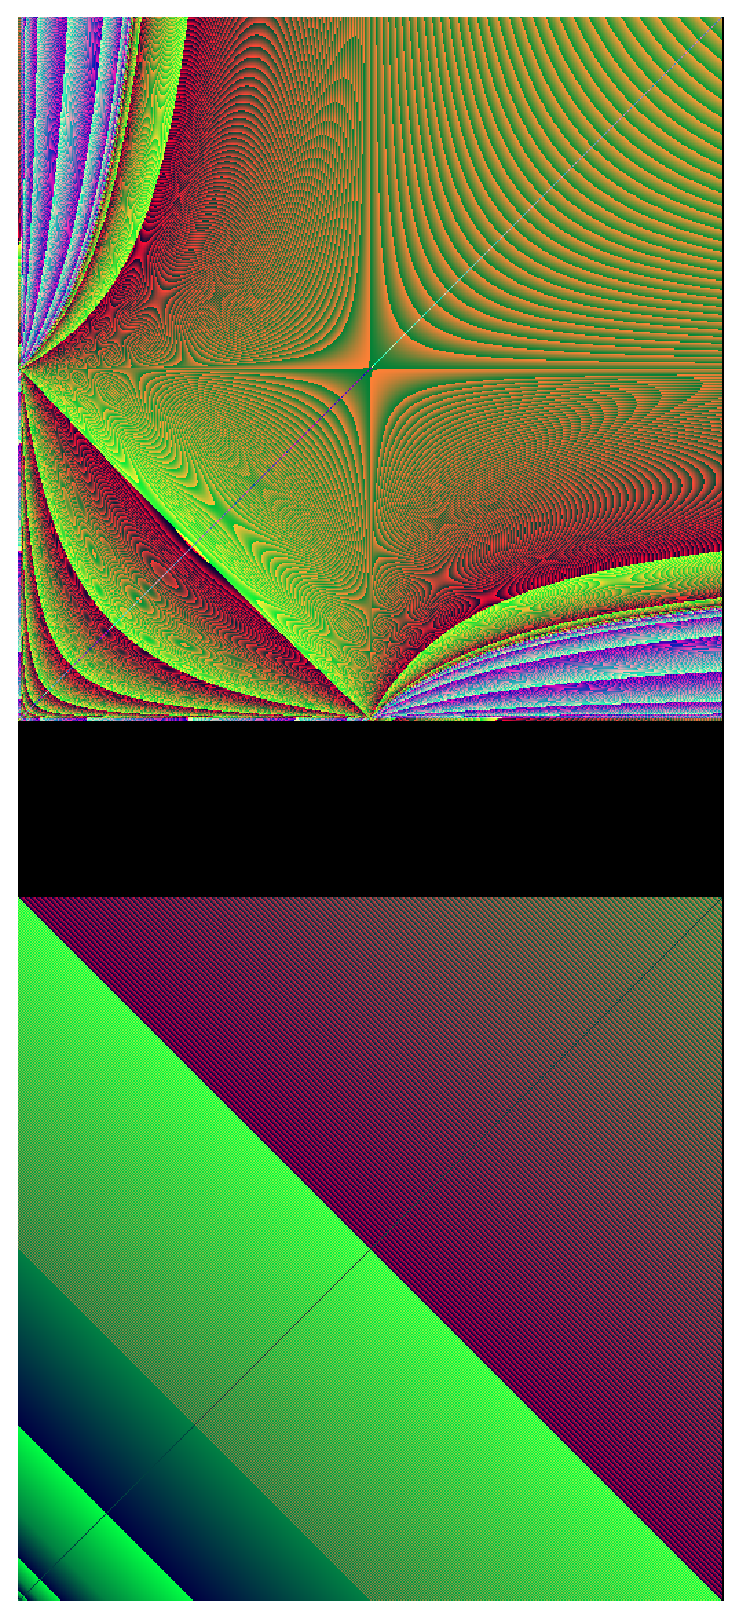
\includegraphics[angle=270,origin=b,width=0.80\textwidth]{inv.eps}
\caption{Inverse matrix}
\end{figure}

512x512�εչ���׻���LUʬ��ˤǤ��롥���٤ΥС����ȱ黻�ˤ��8��ʬ��׻���
�롥���ƥ󥷥�׻��ǤϤʤ�mapdist=0�Ǥ��롥

\begin{screen}
\tiny
\begin{verbatim}
  /* LUʬ�� */
  for (i=0; i<M+1; i++)
    p[i] = i;
  for (i=0; i<M; i++) {
    pmax = 0.0;
    k = -1;
    for (j=i; j<M; j++) {
      if (pmax < fabsf(A[p[j]*M+i])) {
        pmax = fabsf(A[p[j]*M+i]);
        k = j;
      }
    }
    if (k == -1) {
      fprintf(stderr, "can't solve\n");
      exit(1);
    }
    j = p[k]; p[k] = p[i]; p[i] = j;
    A[p[i]*M+i] = 1.0/A[p[i]*M+i];
    for (j=i+1; j<M; j++) {
      A[p[j]*M+i] *= A[p[i]*M+i];
      for (k=i+1; k<M; k++)
        A[p[j]*M+k] -= A[p[j]*M+i]*A[p[i]*M+k];
    }
  }
\end{verbatim}
\end{screen}

\begin{screen}
\tiny
\begin{verbatim}
  /* LUʬ�� */
  for (i=0; i<M+1; i++)
    p[i] = i;
  for (i=0; i<M; i++) { /* ������ */
    pmax = 0.0;
    k = -1;
    for (j=i; j<M; j++) { /* ��������õ�� */
      if (pmax < fabsf(A[p[j]*M+i])) {
        pmax = fabsf(A[p[j]*M+i]);
        k = j;
      }
    }
    if (k == -1) {
      fprintf(stderr, "can't solve\n");
      exit(1);
    }
    j = p[k]; p[k] = p[i]; p[i] = j;
    A[p[i]*M+i] = 1.0/A[p[i]*M+i];
    for (j=i+1; j<M; j++) /* ������ */
      A[p[j]*M+i] *= A[p[i]*M+i];
    for (j=i+1; j<M; j+=NCHIP*H) { /* ������ */
      /********************************************/
      for (CHIP=0; CHIP<NCHIP; CHIP++) {
        for (k=0; k<M-(i+1); k++) { /* ���������� */
          for (h=0; h<H; h++) { /* vertical (parallel) execution */
            if (j+h*NCHIP+CHIP<M) A[p[j+h*NCHIP+CHIP]*M+i+1+k] -= A[p[j+h*NCHIP+CHIP]*M+i]*A[p[i]*M+i+1+k];
                                                     /* ��³�εչ���Ȱۤʤ�,accumurate�ǤϤʤ��������ñ�ȸ����η��֤� */
                                                     /* const:A[p[j]][0] * LMM A[p[  0]][*] */
                                                     /*        ��                           */
            /*   v A[p[j]*M+i]         */            /*   LMM A[p[j>0]][*] accumulate (column������j,j+1,..,479�Τ����¸̵) */
            /***************************/
            /* + - - - - - - - - - - - */ /* A[p[i]] ��Ƭ��       */ /* ��Ƭ�Ԥ�i�����ޤǺ����Ѳ�ǽ */
            /* | * > > > > > > > > > > */ /* A[p[j]] ���Ԥ������ */ /* 1�Ԥ�LMM�˼��� */
            /* | v + - - - - - - - - - */
            /* | v | * > > > > > > > > */ /* M/60����Ƥ���i�����ޤ�j+=60�򷫤��֤� */
            /* | v | v + - - - - - - - */ /* ���ֹ���Ӥ�cst�ˤ��ü������ */
            /* | v | v - + - - - - - - */ /* + CHIP#1 h=0 */
            /* | v | v - - + - - - - - */ /* + CHIP#0 h=1 */
            /* | v | v - - - + - - - - */ /* + CHIP#1 h=1 */
            /* | v | v - - - - + - - - */ /* + CHIP#0 h=2 */
            /* | v | v - - - - - + - - */ /* + CHIP#1 h=2 */
            /* | v | v - - - - - - + - */ /* + CHIP#0 h=3 */
            /* | v | v - - - - - - - + */ /* + CHIP#1 h=3 */
            /***************************/ /* ����60�ԤޤǼ�����ǽ */
          }
        }
      }
      /********************************************/
    }
  }
\end{verbatim}
\end{screen}

\begin{screen}
\tiny
\begin{verbatim}
  /* LUʬ�� */
  for (i=0; i<M+1; i++)
    p[i] = i;
  for (i=0; i<M; i++) { /* ������ */
    pmax = 0.0;
    k = -1;
    for (j=i; j<M; j++) { /* ��������õ�� */
      if (pmax < fabsf(A[j*M+i])) {
        pmax = fabsf(A[j*M+i]);
        k = j;
      }
    }
    if (k == -1) {
      fprintf(stderr, "can't solve\n");
      exit(1);
    }
    j = p[k]; p[k] = p[i]; p[i] = j;
    for (j=0; j<M; j++) { /* real pivotting */            /*��*/
      tmp = A[k*M+j]; A[k*M+j] = A[i*M+j]; A[i*M+j] = tmp;/*��*/
    }                                                     /*��*/
    A[i*M+i] = 1.0/A[i*M+i];                              /*��*/
    for (j=i+1; j<M; j++) /* ������ */
      A[j*M+i] *= A[i*M+i];

    Uint *top  = &A[i*M+i];
    Uint *topw = (Ull)top;
    Uint  len  = M-i;
    Uint  len2 = len+(RMGRP-1)*M;
    Uint  grp;
    /* FPGA�µ���j-loop�κǽ�(len=1)��ư���ʤ��Τ�,�Ĥ��Ǥ�ARM�Τۤ���®������len��ARM�Ǽ¹� 2019/3/1 Nakashima */
    if (len < 16) { /* len<1�Ǥ�����ʤΤ���ǽ���粽�Ƿ��Ƥ褤 */
      for (j=i+1; j<M; j+=NCHIP*H*RMGRP) { /* ������ */
        for (CHIP=0; CHIP<NCHIP; CHIP++) {
          for (h=0; h<H; h++) { /* vertical (parallel) execution */
            for (grp=0; grp<RMGRP; grp++) {
              for (k=0; k<M-(i+1); k++) { /* ���������� */
                if (j+h*NCHIP*RMGRP+CHIP*RMGRP+grp<M) A[(j+h*NCHIP*RMGRP+CHIP*RMGRP+grp)*M+i+1+k] -= A[(j+h*NCHIP*RMGRP+CHIP*RMGRP+grp)*M+i]*A[i*M+i+1+k];
    } } } } } }
    else {
    for (j=i+1; j<M; j+=NCHIP*H*RMGRP) { /* ������ */
      /********************************************/
      Uint  l00[NCHIP],  l01[NCHIP],  l02[NCHIP],  l03[NCHIP],  l04[NCHIP],  l05[NCHIP],  l06[NCHIP],  l07[NCHIP]; /* j<M-(h*NCHIP+CHIP) */
      Uint  l08[NCHIP],  l09[NCHIP],  l10[NCHIP],  l11[NCHIP],  l12[NCHIP],  l13[NCHIP],  l14[NCHIP],  l15[NCHIP]; /* j<M-(h*NCHIP+CHIP) */
      Uint *d00[NCHIP], *d01[NCHIP], *d02[NCHIP], *d03[NCHIP], *d04[NCHIP], *d05[NCHIP], *d06[NCHIP], *d07[NCHIP]; /* A[p[j+h*NCHIP+CHIP]*M+k] */
      Uint *d08[NCHIP], *d09[NCHIP], *d10[NCHIP], *d11[NCHIP], *d12[NCHIP], *d13[NCHIP], *d14[NCHIP], *d15[NCHIP]; /* A[p[j+h*NCHIP+CHIP]*M+k] */
      Uint *d00w[NCHIP],*d01w[NCHIP],*d02w[NCHIP],*d03w[NCHIP],*d04w[NCHIP],*d05w[NCHIP],*d06w[NCHIP],*d07w[NCHIP];/* A[p[j+h*NCHIP+CHIP]*M+k] */
      Uint *d08w[NCHIP],*d09w[NCHIP],*d10w[NCHIP],*d11w[NCHIP],*d12w[NCHIP],*d13w[NCHIP],*d14w[NCHIP],*d15w[NCHIP];/* A[p[j+h*NCHIP+CHIP]*M+k] */
      for (CHIP=0; CHIP<NCHIP; CHIP++) { /* output channels are parallelized by multi-chip (OC/#chip) */
        l00[CHIP]=(j+ 0*NCHIP*RMGRP+CHIP*RMGRP<M)?(j+ 0*NCHIP*RMGRP+CHIP*RMGRP):M;l01[CHIP]=(j+ 1*NCHIP*RMGRP+CHIP*RMGRP<M)?(j+ 1*NCHIP*RMGRP+CHIP*RMGRP):M;
                :
        l14[CHIP]=(j+14*NCHIP*RMGRP+CHIP*RMGRP<M)?(j+14*NCHIP*RMGRP+CHIP*RMGRP):M;l15[CHIP]=(j+15*NCHIP*RMGRP+CHIP*RMGRP<M)?(j+15*NCHIP*RMGRP+CHIP*RMGRP):M;
        d00[CHIP] = &A[l00[CHIP]*M+i];   d01[CHIP] = &A[l01[CHIP]*M+i];
                :
        d14[CHIP] = &A[l14[CHIP]*M+i];   d15[CHIP] = &A[l15[CHIP]*M+i];
        d00w[CHIP]= (Ull)d00[CHIP];      d01w[CHIP]= (Ull)d01[CHIP];
                :
        d14w[CHIP]= (Ull)d14[CHIP];      d15w[CHIP]= (Ull)d15[CHIP];
      }
//EMAX5A begin inv_x1 mapdist=0
/*3*/ for (CHIP=0; CHIP<NCHIP; CHIP++) {
  /*2*/ for (INIT1=1,LOOP1=RMGRP,rofs=0-M*4; LOOP1--; INIT1=0) {                             /* stage#0 *//* mapped to FOR() on BR[63][1][0] */
    /*1*/ for (INIT0=1,LOOP0=M-(i+1),cofs=0; LOOP0--; INIT0=0) { /* stage#0 *//* mapped to FOR() on BR[63][0][0] */
            exe(OP_ADD, &cofs, INIT0?cofs:cofs, EXP_H3210, 4LL, EXP_H3210, 0LL, EXP_H3210, OP_AND, 0x00000000ffffffffLL, OP_NOP, 0LL); /* stage#0 */
            exe(OP_ADD, &rofs, rofs, EXP_H3210, INIT0?M*4:0, EXP_H3210, 0LL, EXP_H3210, OP_NOP, 0LL, OP_NOP, 0LL);                     /* stage#0 */
            exe(OP_ADD, &oofs, rofs, EXP_H3210, cofs, EXP_H3210, 0LL, EXP_H3210, OP_AND, 0x00000000ffffffffLL, OP_NOP, 0LL);           /* stage#1 */
            exe(OP_CMP_LT,   &cc0,         l00[CHIP],   EXP_H3210, M,         EXP_H3210, 0LL,         EXP_H3210, OP_NOP, 0LL, OP_NOP, 0LL); /* stage#1              LD
            mop(OP_LDWR,  1, &BR[2][2][1], top,         cofs, MSK_W0, topw,       len, 0, 0, NULL, len);  /* A[p[i]*M+k]                       stage#2              |
            mop(OP_LDWR,  1, &BR[2][0][1], d00[CHIP],   oofs, MSK_W0, d00w[CHIP], len2,0, 1, NULL, len2); /* A[p[j+h*NCHIP+CHIP]*M+k]          stage#2  +->         |
            mop(OP_LDWR,  1, &BR[2][1][1], d00[CHIP],   rofs, MSK_W0, d00w[CHIP], len2,0, 1, NULL, len2); /* A[p[j+h*NCHIP+CHIP]*M+k]          stage#2  +->         |
            exe(OP_FMS,      &AR[2][0],    BR[2][0][1], EXP_H3210, BR[2][1][1], EXP_H3210, BR[2][2][1], EXP_H3210, OP_NOP, 0LL, OP_NOP, 0); /* stage#2  |   ������  |
            cex(OP_CEXE,     &ex0,   0, 0, 0, cc0, 0xaaaa);                                                                                 /* stage#2  |  AR[1]    |
            mop(OP_STWR,ex0, &AR[2][0],    oofs,   d00[CHIP], MSK_D0, d00w[CHIP], len2, 0, 1, NULL, len2);                                  /* stage#2  |    + ST   v
#if (H>1)                                                                                                                                   /*          *--------- BR[2]
            exe(OP_CMP_LT,   &cc0,         l01[CHIP],   EXP_H3210, M,         EXP_H3210, 0LL,         EXP_H3210, OP_NOP, 0LL, OP_NOP, 0LL); /* stage#2              LD
            mop(OP_LDWR,  1, &BR[3][2][1], top,         cofs, MSK_W0, topw,       len, 0, 0, NULL, len);  /* A[p[i]*M+k]                       stage#3              |
            mop(OP_LDWR,  1, &BR[3][0][1], d01[CHIP],   oofs, MSK_W0, d01w[CHIP], len2,0, 1, NULL, len2); /* A[p[j+h*NCHIP+CHIP]*M+k]          stage#3  +->         |
            mop(OP_LDWR,  1, &BR[3][1][1], d01[CHIP],   rofs, MSK_W0, d01w[CHIP], len2,0, 1, NULL, len2); /* A[p[j+h*NCHIP+CHIP]*M+k]          stage#3  +->         |
            exe(OP_FMS,      &AR[3][0],    BR[3][0][1], EXP_H3210, BR[3][1][1], EXP_H3210, BR[3][2][1], EXP_H3210, OP_NOP, 0LL, OP_NOP, 0); /* stage#3  |   ������  |
            cex(OP_CEXE,     &ex0,   0, 0, 0, cc0, 0xaaaa);                                                                                 /* stage#3  |  AR[2]    |
            mop(OP_STWR,ex0, &AR[3][0],    oofs,   d01[CHIP], MSK_D0, d01w[CHIP], len2, 0, 1, NULL, len2);                                  /* stage#3  |    + ST   v
                :
#if (H>12)                                                                                                                                  /*          *--------- BR[13]
            exe(OP_CMP_LT,   &cc0,         l12[CHIP],   EXP_H3210, M,         EXP_H3210, 0LL,         EXP_H3210, OP_NOP, 0LL, OP_NOP, 0LL); /* stage#13             LD
            mop(OP_LDWR,  1, &BR[14][2][1],top,         cofs, MSK_W0, topw,       len, 0, 0, NULL, len);  /* A[p[i]*M+k] stage#1               stage#14             |
            mop(OP_LDWR,  1, &BR[14][0][1],d12[CHIP],   oofs, MSK_W0, d12w[CHIP], len2,0, 1, NULL, len2); /* A[p[j+h*NCHIP+CHIP]*M+k]          stage#14 +->         |
            mop(OP_LDWR,  1, &BR[14][1][1],d12[CHIP],   rofs, MSK_W0, d12w[CHIP], len2,0, 1, NULL, len2); /* A[p[j+h*NCHIP+CHIP]*M+k]          stage#14 +->         |
            exe(OP_FMS,      &AR[14][0],   BR[14][0][1],EXP_H3210, BR[14][1][1], EXP_H3210, BR[14][2][1],EXP_H3210, OP_NOP, 0LL, OP_NOP, 0);/* stage#14 |   ������  |
            cex(OP_CEXE,     &ex0,   0, 0, 0, cc0, 0xaaaa);                                                                                 /* stage#14 |  AR[13]   |
            mop(OP_STWR,ex0, &AR[14][0],   oofs,   d12[CHIP], MSK_D0, d12w[CHIP], len2, 0, 1, NULL, len2);                                  /* stage#14 |    + ST   v
#if (H>13)                                                                                                                                  /*          *--------- BR[14]
            exe(OP_CMP_LT,   &cc0,         l13[CHIP],   EXP_H3210, M,         EXP_H3210, 0LL,         EXP_H3210, OP_NOP, 0LL, OP_NOP, 0LL); /* stage#14             LD
            mop(OP_LDWR,  1, &BR[15][2][1],top,         cofs, MSK_W0, topw,       len, 0, 0, NULL, len);  /* A[p[i]*M+k] stage#1               stage#15             |
            mop(OP_LDWR,  1, &BR[15][0][1],d13[CHIP],   oofs, MSK_W0, d13w[CHIP], len2,0, 1, NULL, len2); /* A[p[j+h*NCHIP+CHIP]*M+k]          stage#15 +->         |
            mop(OP_LDWR,  1, &BR[15][1][1],d13[CHIP],   rofs, MSK_W0, d13w[CHIP], len2,0, 1, NULL, len2); /* A[p[j+h*NCHIP+CHIP]*M+k]          stage#15 +->         |
            exe(OP_FMS,      &AR[15][0],   BR[15][0][1],EXP_H3210, BR[15][1][1], EXP_H3210, BR[15][2][1],EXP_H3210, OP_NOP, 0LL, OP_NOP, 0);/* stage#15 |   ������  |
            cex(OP_CEXE,     &ex0,   0, 0, 0, cc0, 0xaaaa);                                                                                 /* stage#15 |  AR[14]   |
            mop(OP_STWR,ex0, &AR[15][0],   oofs,   d13[CHIP], MSK_D0, d13w[CHIP], len2, 0, 1, NULL, len2);                                  /* stage#15 |    + ST   v
#if (H>14)                                                                                                                                  /*          *--------- BR[15]
            exe(OP_CMP_LT,   &cc0,         l14[CHIP],   EXP_H3210, M,         EXP_H3210, 0LL,         EXP_H3210, OP_NOP, 0LL, OP_NOP, 0LL); /* stage#15             LD
            mop(OP_LDWR,  1, &BR[16][2][1],top,         cofs, MSK_W0, topw,       len, 0, 0, NULL, len);  /* A[p[i]*M+k] stage#1               stage#16             |
            mop(OP_LDWR,  1, &BR[16][0][1],d14[CHIP],   oofs, MSK_W0, d14w[CHIP], len2,0, 1, NULL, len2); /* A[p[j+h*NCHIP+CHIP]*M+k]          stage#16 +->         |
            mop(OP_LDWR,  1, &BR[16][1][1],d14[CHIP],   rofs, MSK_W0, d14w[CHIP], len2,0, 1, NULL, len2); /* A[p[j+h*NCHIP+CHIP]*M+k]          stage#16 +->         |
            exe(OP_FMS,      &AR[16][0],   BR[16][0][1],EXP_H3210, BR[16][1][1], EXP_H3210, BR[16][2][1],EXP_H3210, OP_NOP, 0LL, OP_NOP, 0);/* stage#16 |   ������  |
            cex(OP_CEXE,     &ex0,   0, 0, 0, cc0, 0xaaaa);                                                                                 /* stage#16 |  AR[15]   |
            mop(OP_STWR,ex0, &AR[16][0],   oofs,   d14[CHIP], MSK_D0, d14w[CHIP], len2, 0, 1, NULL, len2);                                  /* stage#16 |    + ST   v
#if (H>15)                                                                                                                                  /*          *--------- BR[16]
            exe(OP_CMP_LT,   &cc0,         l15[CHIP],   EXP_H3210, M,         EXP_H3210, 0LL,         EXP_H3210, OP_NOP, 0LL, OP_NOP, 0LL); /* stage#16             LD
            mop(OP_LDWR,  1, &BR[17][2][1],top,         cofs, MSK_W0, topw,       len, 0, 0, NULL, len);  /* A[p[i]*M+k] stage#1               stage#17             |
            mop(OP_LDWR,  1, &BR[17][0][1],d15[CHIP],   oofs, MSK_W0, d15w[CHIP], len2,0, 1, NULL, len2); /* A[p[j+h*NCHIP+CHIP]*M+k]          stage#17 +->         |
            mop(OP_LDWR,  1, &BR[17][1][1],d15[CHIP],   rofs, MSK_W0, d15w[CHIP], len2,0, 1, NULL, len2); /* A[p[j+h*NCHIP+CHIP]*M+k]          stage#17 +->         |
            exe(OP_FMS,      &AR[17][0],   BR[17][0][1],EXP_H3210, BR[17][1][1], EXP_H3210, BR[17][2][1],EXP_H3210, OP_NOP, 0LL, OP_NOP, 0);/* stage#17 |   ������  |
            cex(OP_CEXE,     &ex0,   0, 0, 0, cc0, 0xaaaa);                                                                                 /* stage#17 |  AR[16]   |
            mop(OP_STWR,ex0, &AR[17][0],   oofs,   d15[CHIP], MSK_D0, d15w[CHIP], len2, 0, 1, NULL, len2);                                  /* stage#17 |    + ST   v
                                                                                                                                            /*          *--------- BR[17]
#endif
      } } }
//EMAX5A end
      /********************************************/
    } /* j-loop */
//EMAX5A drain_dirty_lmm
\end{verbatim}
\end{screen}

\begin{figure}[htbp]
\center
\epsfile{file=inv+rmm-inv_x1-emax6.eps,width=1.00\textwidth}
\caption{�չ���(1/3)}
\end{figure}

\clearpage

\subsection{�չ���(2/3)}

512x512�εչ���׻������ʾõ�ˤǤ��롥���٤ΥС����ȱ黻�ˤ��8��ʬ��׻���
�롥���ƥ󥷥�׻��ǤϤʤ�mapdist=0�Ǥ��롥

\begin{screen}
\tiny
\begin{verbatim}
  /* �չ�����Ⱦ */
  for (i=0; i<M; i++) {
    for (j=0; j<M; j++)
      b[p[j]] = (i==j)?1.0:0.0;
    /*for (j=1; j<M; j++) { *//*�̾��ϢΩ����������ξ��*/
    for (j=i+1; j<M; j++) { /* �չ���(b[]=E)�ξ��,k<i�Ǥ�b[]==0�ʤΤ�j=i+1���鳫�� */
      /*for (k=0; k<j; k++) *//*�̾��ϢΩ����������ξ��*/
      for (k=i; k<j; k++) /* �չ���(b[]=E)�ξ��,k<i�Ǥ�b[]==0�ʤΤ�k=i���鳫�� */
        b[p[j]] -= A[p[j]*M+k]*b[p[k]];
    }
  }
\end{verbatim}
\end{screen}

\begin{screen}
\tiny
\begin{verbatim}
  /* �չ������ */
  for (i=0; i<M; i++) { /* ������ */
    for (j=0; j<M; j++) /* ������ */
      b[i*M+j] = (i==j)?1.0:0.0;
  }
  for (i=0; i<M; i+=NCHIP*H) { /* ������ */
    for (j=1; j<M; j++) { /* ������ */
      /********************************************/
      for (CHIP=0; CHIP<NCHIP; CHIP++) {
        for (k=0; k<j; k++) { /* ���������� */
          for (h=0; h<H; h++) { /* vertical (parallel) execution */
            b[(i+CHIP*H+h)*M+j] -= A[p[j]*M+k]*b[(i+CHIP*H+h)*M+k];
                                        /* b[*]��Ĥ����֤�����,A�������. j�����������б����뤬�������ΰ�ư��k��Ĺ���ʤ� */
                                        /* ����Ĺk��H������Ÿ����������Τ��񤷤�.k��read-modify-write�β�ž���˼������뤷���ʤ� */
                                        /* b[*]��A[j][*]��Ʊ��LMM���������� ����64KB/4/2=��8K����,b[*]�򤤤���ư�����ʤ��� */
                                        /* ��ž��j�����Ŭ�Ѥ���ˤ�,i��WxH������Ÿ������Τ����� */
              /*           ����A[p[j]][*]��broadcast��ǽ ��A[p[j]][*]��p[j]����Ϣ³�ʤΤ�1K���ǤޤǼ���.�Ĥޤ���ť롼��Ÿ����̵�� */
              /* +-----------------------------------+     +------+ +------+ +------+ */
              /* b[ 3][j]-=A[p[j]][0:j-1] b[ 3][0:j-1]     b[ 2][*] b[ 1][*] b[ 0][*] */
              /*                                                                      */
              /* b[ 7][j]-=A[p[j]][0:j-1] b[ 7][0:j-1]     b[ 6][*] b[ 5][*] b[ 4][*] */
              /* b[59][j]-=A[p[j]][0:j-1] b[59][0:j-1]     b[58][*] b[57][*] b[56][*] */
          }
        }
      }
      /********************************************/
    }
  }
\end{verbatim}
\end{screen}

\begin{screen}
\tiny
\begin{verbatim}
  /* �չ�����Ⱦ */
  for (i=0; i<M; i++) { /* ������ */
    for (j=0; j<M; j++) /* ������ */
      b[i*M+j] = (i==j)?1.0:0.0;
  }
  for (i=0; i<M; i+=NCHIP*H) { /* ������ */
    /*for (j=1; j<M; j++) { *//*�̾��ϢΩ����������ξ��*/
    for (j=i+1; j<M; j++) { /* �չ���(b[]=E)�ξ��,k<i�Ǥ�b[]==0�ʤΤ�j=i+1���鳫�� */
      Uint *top  = &A[p[j]*M+i];                                     /* A[p[j]*M+k] */
      Uint *topw = (Ull)top;
      /*Uint  len = (j+1)/2;*/
      Uint  len = j-i;/* b��ñ�̹���ξ��,k<i�Ǥ�b[]==0�ʤΤ�k=i���鳫�� */
      /********************************************/
      if (len < 2) { /* len<1�Ǥ�����ʤΤ���ǽ���粽�Ƿ��Ƥ褤 */
        for (CHIP=0; CHIP<NCHIP; CHIP++) {
        /*for (k=0; k<j; k++) { *//*�̾��ϢΩ����������ξ��*/
          for (k=i; k<j; k++) { /* �չ���(b[]=E)�ξ��,k<i�Ǥ�b[]==0�ʤΤ�k=i���鳫�� */
            for (h=0; h<H; h++) { /* vertical (parallel) execution */
              b[(i+CHIP*H+h)*M+j] -= A[p[j]*M+k]*b[(i+CHIP*H+h)*M+k];
            }
          }
        }
      }
      else {
      Uint  jc = j-i;
      Ull   Ajk; /* k=0...j-1 */
      Ull   b000, b001;
      Uint  l000[NCHIP],  l010[NCHIP],  l020[NCHIP],  l030[NCHIP],  l040[NCHIP],  l050[NCHIP],  l060[NCHIP],  l070[NCHIP];  /* (i+CHIP*W*H+h*W+w)        */
      Uint  l080[NCHIP],  l090[NCHIP],  l100[NCHIP],  l110[NCHIP],  l120[NCHIP],  l130[NCHIP],  l140[NCHIP],  l150[NCHIP];  /* (i+CHIP*W*H+h*W+w)        */
      Uint *t000[NCHIP], *t010[NCHIP], *t020[NCHIP], *t030[NCHIP], *t040[NCHIP], *t050[NCHIP], *t060[NCHIP], *t070[NCHIP];  /* b[(i+CHIP*W*H+h*W+w)*M+k] */
      Uint *t080[NCHIP], *t090[NCHIP], *t100[NCHIP], *t110[NCHIP], *t120[NCHIP], *t130[NCHIP], *t140[NCHIP], *t150[NCHIP];  /* b[(i+CHIP*W*H+h*W+w)*M+k] */
      Uint *t000w[NCHIP],*t010w[NCHIP],*t020w[NCHIP],*t030w[NCHIP],*t040w[NCHIP],*t050w[NCHIP],*t060w[NCHIP],*t070w[NCHIP]; /* b[(i+CHIP*W*H+h*W+w)*M+k] */
      Uint *t080w[NCHIP],*t090w[NCHIP],*t100w[NCHIP],*t110w[NCHIP],*t120w[NCHIP],*t130w[NCHIP],*t140w[NCHIP],*t150w[NCHIP]; /* b[(i+CHIP*W*H+h*W+w)*M+k] */
      Uint *d000[NCHIP], *d010[NCHIP], *d020[NCHIP], *d030[NCHIP], *d040[NCHIP], *d050[NCHIP], *d060[NCHIP], *d070[NCHIP];  /* b[(i+CHIP*W*H+h*W+w)*M+j] */
      Uint *d080[NCHIP], *d090[NCHIP], *d100[NCHIP], *d110[NCHIP], *d120[NCHIP], *d130[NCHIP], *d140[NCHIP], *d150[NCHIP];  /* b[(i+CHIP*W*H+h*W+w)*M+j] */
      Uint *d000w[NCHIP],*d010w[NCHIP],*d020w[NCHIP],*d030w[NCHIP],*d040w[NCHIP],*d050w[NCHIP],*d060w[NCHIP],*d070w[NCHIP]; /* b[(i+CHIP*W*H+h*W+w)*M+j] */
      Uint *d080w[NCHIP],*d090w[NCHIP],*d100w[NCHIP],*d110w[NCHIP],*d120w[NCHIP],*d130w[NCHIP],*d140w[NCHIP],*d150w[NCHIP]; /* b[(i+CHIP*W*H+h*W+w)*M+j] */
      for (CHIP=0; CHIP<NCHIP; CHIP++) { /* output channels are parallelized by multi-chip (OC/#chip) */
        l000[CHIP] = (i+CHIP*H+ 0+0)*M;         l010[CHIP] = (i+CHIP*H+ 1+0)*M;         l020[CHIP] = (i+CHIP*H+ 2+0)*M;         l030[CHIP] = (i+CHIP*H+ 3+0)*M;
              :
        l120[CHIP] = (i+CHIP*H+12+0)*M;         l130[CHIP] = (i+CHIP*H+13+0)*M;         l140[CHIP] = (i+CHIP*H+14+0)*M;         l150[CHIP] = (i+CHIP*H+15+0)*M;
        t000[CHIP] = &b[l000[CHIP]+i]; t010[CHIP] = &b[l010[CHIP]+i];
              :
        t140[CHIP] = &b[l140[CHIP]+i]; t150[CHIP] = &b[l150[CHIP]+i];
        t000w[CHIP]= (Ull)t000[CHIP];  t010w[CHIP]= (Ull)t010[CHIP];
              :
        t140w[CHIP]= (Ull)t140[CHIP];  t150w[CHIP]= (Ull)t150[CHIP];
        d000[CHIP] = &b[l000[CHIP]+j]; d010[CHIP] = &b[l010[CHIP]+j];
              :
        d140[CHIP] = &b[l140[CHIP]+j]; d150[CHIP] = &b[l150[CHIP]+j];
        d000w[CHIP]= (Ull)d000[CHIP];  d010w[CHIP]= (Ull)d010[CHIP];
              :
        d140w[CHIP]= (Ull)d140[CHIP];  d150w[CHIP]= (Ull)d150[CHIP];
      }
//EMAX5A begin inv_x2 mapdist=0
/*2*/ for (CHIP=0; CHIP<NCHIP; CHIP++) {
  /*1*/ for (INIT0=1,LOOP0=jc,cofs=0-4; LOOP0--; INIT0=0) { /* stage#0 *//* mapped to FOR() on BR[63][0][0] */
          exe(OP_ADD, &cofs, cofs, EXP_H3210, 4LL, EXP_H3210, 0LL, EXP_H3210, OP_AND, 0x00000000ffffffffLL, OP_NOP, 0LL); /* stage#0 */
          mop(OP_LDWR,  1, &Ajk,         top,          cofs, MSK_W0, topw,        len, 0, 0, NULL, len);  /* A[p[j]*M+k]              */
          mop(OP_LDWR,  1, &BR[1][3][1], t000[CHIP],   cofs, MSK_W0, t000w[CHIP], len, 0, 1, NULL, len);  /* b[(i+CHIP*W*H+h*W+0)*M+k]*//* stage#1.3 +->xxx     LD */
          mop(OP_LDWR,  1, &b000,        d000[CHIP],   0,    MSK_W0, d000w[CHIP], 1,   0, 1, NULL, 1);    /* b[(i+CHIP*W*H+h*W+0)*M+j]*//* stage#2.0 |   ������ |  */
          exe(OP_FMS,      &b000,        b000,         EXP_H3210, Ajk, EXP_H3210, BR[1][3][1], EXP_H3210, OP_NOP, 0LL, OP_NOP, 0LL);    /* stage#2.0 +- xxx+ST  v  */
          mop(OP_STWR,  1, &b000,        0,      d000[CHIP], MSK_D0, d000w[CHIP], 1,   0, 1, NULL, 1);                                  /* stage#2.0 +-------- xxx */
#if (H>1)
          mop(OP_LDWR,  1, &BR[2][3][1], t010[CHIP],   cofs, MSK_W0, t010w[CHIP], len, 0, 1, NULL, len);  /* b[(i+CHIP*W*H+h*W+1)*M+k]*//* stage#2.3 +->xxx     LD */
          mop(OP_LDWR,  1, &b000,        d010[CHIP],   0,    MSK_W0, d010w[CHIP], 1,   0, 1, NULL, 1);    /* b[(i+CHIP*W*H+h*W+0)*M+j]*//* stage#3.0 |   ������ |  */
          exe(OP_FMS,      &b000,        b000,         EXP_H3210, Ajk, EXP_H3210, BR[2][3][1], EXP_H3210, OP_NOP, 0LL, OP_NOP, 0LL);    /* stage#3.0 +- xxx+ST  v  */
          mop(OP_STWR,  1, &b000,        0,      d010[CHIP], MSK_D0, d010w[CHIP], 1,   0, 1, NULL, 1);                                  /* stage#3.0 +-------- xxx */
                :
#if (H>8)
          mop(OP_LDWR,  1, &BR[9][3][1], t080[CHIP],   cofs, MSK_W0, t080w[CHIP], len, 0, 1, NULL, len);  /* b[(i+CHIP*W*H+h*W+0)*M+k]*//* stage#9.3 +->xxx     LD */
          mop(OP_LDWR,  1, &b000,        d080[CHIP],   0,    MSK_W0, d080w[CHIP], 1,   0, 1, NULL, 1);    /* b[(i+CHIP*W*H+h*W+0)*M+j]*//* stage#10.0|   ������ |  */
          exe(OP_FMS,      &b000,        b000,         EXP_H3210, Ajk, EXP_H3210, BR[9][3][1], EXP_H3210, OP_NOP, 0LL, OP_NOP, 0LL);    /* stage#10.0+- xxx+ST  v  */
          mop(OP_STWR,  1, &b000,        0,      d080[CHIP], MSK_D0, d080w[CHIP], 1,   0, 1, NULL, 1);                                  /* stage#10.0+-------- xxx */
#if (H>9)
          mop(OP_LDWR,  1, &BR[10][3][1],t090[CHIP],   cofs, MSK_W0, t090w[CHIP], len, 0, 1, NULL, len);  /* b[(i+CHIP*W*H+h*W+0)*M+k]*//* stage#10.3+->xxx     LD */
          mop(OP_LDWR,  1, &b000,        d090[CHIP],   0,    MSK_W0, d090w[CHIP], 1,   0, 1, NULL, 1);    /* b[(i+CHIP*W*H+h*W+0)*M+j]*//* stage#11.0|   ������ |  */
          exe(OP_FMS,      &b000,        b000,         EXP_H3210, Ajk, EXP_H3210, BR[10][3][1],EXP_H3210, OP_NOP, 0LL, OP_NOP, 0LL);    /* stage#11.0+- xxx+ST  v  */
          mop(OP_STWR,  1, &b000,        0,      d090[CHIP], MSK_D0, d090w[CHIP], 1,   0, 1, NULL, 1);                                  /* stage#11.0+-------- xxx */
#if (H>10)
          mop(OP_LDWR,  1, &BR[11][3][1],t100[CHIP],   cofs, MSK_W0, t100w[CHIP], len, 0, 1, NULL, len);  /* b[(i+CHIP*W*H+h*W+0)*M+k]*//* stage#11.3+->xxx     LD */
          mop(OP_LDWR,  1, &b000,        d100[CHIP],   0,    MSK_W0, d100w[CHIP], 1,   0, 1, NULL, 1);    /* b[(i+CHIP*W*H+h*W+0)*M+j]*//* stage#12.0|   ������ |  */
          exe(OP_FMS,      &b000,        b000,         EXP_H3210, Ajk, EXP_H3210, BR[11][3][1],EXP_H3210, OP_NOP, 0LL, OP_NOP, 0LL);    /* stage#12.0+- xxx+ST  v  */
          mop(OP_STWR,  1, &b000,        0,      d100[CHIP], MSK_D0, d100w[CHIP], 1,   0, 1, NULL, 1);                                  /* stage#12.0+-------- xxx */
#if (H>11)
          mop(OP_LDWR,  1, &BR[12][3][1],t110[CHIP],   cofs, MSK_W0, t110w[CHIP], len, 0, 1, NULL, len);  /* b[(i+CHIP*W*H+h*W+0)*M+k]*//* stage#12.3+->xxx     LD */
          mop(OP_LDWR,  1, &b000,        d110[CHIP],   0,    MSK_W0, d110w[CHIP], 1,   0, 1, NULL, 1);    /* b[(i+CHIP*W*H+h*W+0)*M+j]*//* stage#13.0|   ������ |  */
          exe(OP_FMS,      &b000,        b000,         EXP_H3210, Ajk, EXP_H3210, BR[12][3][1],EXP_H3210, OP_NOP, 0LL, OP_NOP, 0LL);    /* stage#13.0+- xxx+ST  v  */
          mop(OP_STWR,  1, &b000,        0,      d110[CHIP], MSK_D0, d110w[CHIP], 1,   0, 1, NULL, 1);                                  /* stage#13.0+-------- xxx */
#if (H>12)
          mop(OP_LDWR,  1, &BR[13][3][1],t120[CHIP],   cofs, MSK_W0, t120w[CHIP], len, 0, 1, NULL, len);  /* b[(i+CHIP*W*H+h*W+0)*M+k]*//* stage#13.3+->xxx     LD */
          mop(OP_LDWR,  1, &b000,        d120[CHIP],   0,    MSK_W0, d120w[CHIP], 1,   0, 1, NULL, 1);    /* b[(i+CHIP*W*H+h*W+0)*M+j]*//* stage#14.0|   ������ |  */
          exe(OP_FMS,      &b000,        b000,         EXP_H3210, Ajk, EXP_H3210, BR[13][3][1],EXP_H3210, OP_NOP, 0LL, OP_NOP, 0LL);    /* stage#14.0+- xxx+ST  v  */
          mop(OP_STWR,  1, &b000,        0,      d120[CHIP], MSK_D0, d120w[CHIP], 1,   0, 1, NULL, 1);                                  /* stage#14.0+-------- xxx */
#if (H>13)
          mop(OP_LDWR,  1, &BR[14][3][1],t130[CHIP],   cofs, MSK_W0, t130w[CHIP], len, 0, 1, NULL, len);  /* b[(i+CHIP*W*H+h*W+0)*M+k]*//* stage#14.3+->xxx     LD */
          mop(OP_LDWR,  1, &b000,        d130[CHIP],   0,    MSK_W0, d130w[CHIP], 1,   0, 1, NULL, 1);    /* b[(i+CHIP*W*H+h*W+0)*M+j]*//* stage#15.0|   ������ |  */
          exe(OP_FMS,      &b000,        b000,         EXP_H3210, Ajk, EXP_H3210, BR[14][3][1],EXP_H3210, OP_NOP, 0LL, OP_NOP, 0LL);    /* stage#15.0+- xxx+ST  v  */
          mop(OP_STWR,  1, &b000,        0,      d130[CHIP], MSK_D0, d130w[CHIP], 1,   0, 1, NULL, 1);                                  /* stage#15.0+-------- xxx */
#if (H>14)
          mop(OP_LDWR,  1, &BR[15][3][1],t140[CHIP],   cofs, MSK_W0, t140w[CHIP], len, 0, 1, NULL, len);  /* b[(i+CHIP*W*H+h*W+0)*M+k]*//* stage#15.3+->xxx     LD */
          mop(OP_LDWR,  1, &b000,        d140[CHIP],   0,    MSK_W0, d140w[CHIP], 1,   0, 1, NULL, 1);    /* b[(i+CHIP*W*H+h*W+0)*M+j]*//* stage#16.0|   ������ |  */
          exe(OP_FMS,      &b000,        b000,         EXP_H3210, Ajk, EXP_H3210, BR[15][3][1],EXP_H3210, OP_NOP, 0LL, OP_NOP, 0LL);    /* stage#16.0+- xxx+ST  v  */
          mop(OP_STWR,  1, &b000,        0,      d140[CHIP], MSK_D0, d140w[CHIP], 1,   0, 1, NULL, 1);                                  /* stage#16.0+-------- xxx */
#if (H>15)
          mop(OP_LDWR,  1, &BR[16][3][1],t150[CHIP],   cofs, MSK_W0, t150w[CHIP], len, 0, 1, NULL, len);  /* b[(i+CHIP*W*H+h*W+0)*M+k]*//* stage#16.3+->xxx     LD */
          mop(OP_LDWR,  1, &b000,        d150[CHIP],   0,    MSK_W0, d150w[CHIP], 1,   0, 1, NULL, 1);    /* b[(i+CHIP*W*H+h*W+0)*M+j]*//* stage#17.0|   ������ |  */
          exe(OP_FMS,      &b000,        b000,         EXP_H3210, Ajk, EXP_H3210, BR[16][3][1],EXP_H3210, OP_NOP, 0LL, OP_NOP, 0LL);    /* stage#17.0+- xxx+ST  v  */
          mop(OP_STWR,  1, &b000,        0,      d150[CHIP], MSK_D0, d150w[CHIP], 1,   0, 1, NULL, 1);                                  /* stage#17.0+-------- xxx */
#endif
        }
      }
//EMAX5A end
//EMAX5A drain_dirty_lmm
      } /* else */
      /********************************************/
    } /* j-loop */
  }
\end{verbatim}
\end{screen}

\begin{figure}[htbp]
\center
\epsfile{file=inv+rmm-inv_x2-emax6.eps,width=1.00\textwidth}
\caption{�չ���(2/3)}
\end{figure}

\clearpage

\subsection{�չ���(3/3)}

512x512�εչ���׻��ʸ��������ˤǤ��롥���٤ΥС����ȱ黻�ˤ��8��ʬ��׻���
�롥���ƥ󥷥�׻��ǤϤʤ�mapdist=0�Ǥ��롥

\begin{screen}
\tiny
\begin{verbatim}
  /* �չ����Ⱦ */
  for (i=0; i<M; i++) {
    for (j=M-1; j>=0; j--) {
      for (k=M-1; k>j; k--)
        b[p[j]] -= A[p[j]*M+k]*x[k];
      inv0[j*M+p[i]] = x[j] = b[p[j]]*A[p[j]*M+j];
    }
  }
\end{verbatim}
\end{screen}

\begin{screen}
\tiny
\begin{verbatim}
  for (i=0; i<M; i+=NCHIP*H) { /* ������ */
    for (j=M-1; j>=0; j--) { /* ������ */
      /********************************************/
      for (CHIP=0; CHIP<NCHIP; CHIP++) {
        for (k=M-1; k>j; k--) { /* ���������� */
          for (h=0; h<H; h++) { /* vertical (parallel) execution */
            b[(i+CHIP*H+h)*M+j] -= A[p[j]*M+k]*x[(i+CHIP*H+h)*M+k];
                                            /* x[*]��A[j][*]��Ʊ��LMM���������� ����64KB/4/2=��8K����,x[*]�򤤤���ư�����ʤ��� */
                                            /* ��ž��j�����Ŭ�Ѥ���ˤ�,i��WxH������Ÿ������Τ����� */
            /*           ����A[p[j]][*]��broadcast��ǽ ��A[p[j]][*]��p[j]����Ϣ³�ʤΤ�1K���ǤޤǼ���.�Ĥޤ���ť롼��Ÿ����̵�� */
            /* +-----------------------------------+     +------+ +------+ +------+ */
            /* b[ 3][j]-=A[p[j]][M-1:j+1] x[ 3][M-1:j+1] b[ 2][*] b[ 1][*] b[ 0][*] */
            /*                                                                      */
            /* b[ 7][j]-=A[p[j]][M-1:j+1] x[ 7][M-1:j+1] b[ 6][*] b[ 5][*] b[ 4][*] */
            /* b[59][j]-=A[p[j]][M-1:j+1] x[59][M-1:j+1] b[58][*] b[57][*] b[56][*] */
          }
        }
      }
      /********************************************/
      for (CHIP=0; CHIP<NCHIP; CHIP++) {
        for (h=0; h<H; h++) { /* vertical (parallel) execution */
          inv1[j*M+p[i+CHIP*H+h+w]] = x[(i+CHIP*H+h)*M+j] = A[p[j]*M+j]*b[(i+CHIP*H+h)*M+j]; /* PIO�ˤ�LMM��x[i*M+j]��ľ�ܹ��� */
                                                                                             /* i�Ϥ��Τޤޤ�,j�����ؤ� */
        }
      }
    }
  }
\end{verbatim}
\end{screen}

\begin{screen}
\tiny
\begin{verbatim}
  /* �չ����Ⱦ */
  for (i=0; i<M; i+=NCHIP*H) { /* ������ */
    for (j=M-1; j>=0; j--) { /* ������ */
      if (j<M-1) {
        Uint *top  = &A[p[j]*M+j+1];                                  /* A[p[j]*M+k] */
        Uint *topw = (Ull)top;
        Uint  len = M-j-1;
        /********************************************/
        if (len < 2) { /* len<1�Ǥ�����ʤΤ���ǽ���粽�Ƿ��Ƥ褤 */
          for (CHIP=0; CHIP<NCHIP; CHIP++) {
            for (k=M-1; k>j; k--) { /* ���������� */
              for (h=0; h<H; h++) { /* vertical (parallel) execution */
                b[(i+CHIP*H+h)*M+j] -= A[p[j]*M+k]*x[(i+CHIP*H+h)*M+k];
              }
            }
          }
        }
        else {
        Uint  jc = M-j-1;
        Ull   Ajk; /* k=j+1...M-1 */
        Ull   b000, b001;
        Uint  l000[NCHIP],  l010[NCHIP],  l020[NCHIP],  l030[NCHIP],  l040[NCHIP],  l050[NCHIP],  l060[NCHIP],  l070[NCHIP];  /* (i+CHIP*W*H+h*W+w)        */
        Uint  l080[NCHIP],  l090[NCHIP],  l100[NCHIP],  l110[NCHIP],  l120[NCHIP],  l130[NCHIP],  l140[NCHIP],  l150[NCHIP];  /* (i+CHIP*W*H+h*W+w)        */
        Uint *t000[NCHIP], *t010[NCHIP], *t020[NCHIP], *t030[NCHIP], *t040[NCHIP], *t050[NCHIP], *t060[NCHIP], *t070[NCHIP];  /* b[(i+CHIP*W*H+h*W+w)*M+k] */
        Uint *t080[NCHIP], *t090[NCHIP], *t100[NCHIP], *t110[NCHIP], *t120[NCHIP], *t130[NCHIP], *t140[NCHIP], *t150[NCHIP];  /* b[(i+CHIP*W*H+h*W+w)*M+k] */
        Uint *t000w[NCHIP],*t010w[NCHIP],*t020w[NCHIP],*t030w[NCHIP],*t040w[NCHIP],*t050w[NCHIP],*t060w[NCHIP],*t070w[NCHIP]; /* b[(i+CHIP*W*H+h*W+w)*M+k] */
        Uint *t080w[NCHIP],*t090w[NCHIP],*t100w[NCHIP],*t110w[NCHIP],*t120w[NCHIP],*t130w[NCHIP],*t140w[NCHIP],*t150w[NCHIP]; /* b[(i+CHIP*W*H+h*W+w)*M+k] */
        Uint *d000[NCHIP], *d010[NCHIP], *d020[NCHIP], *d030[NCHIP], *d040[NCHIP], *d050[NCHIP], *d060[NCHIP], *d070[NCHIP];  /* b[(i+CHIP*W*H+h*W+w)*M+j] */
        Uint *d080[NCHIP], *d090[NCHIP], *d100[NCHIP], *d110[NCHIP], *d120[NCHIP], *d130[NCHIP], *d140[NCHIP], *d150[NCHIP];  /* b[(i+CHIP*W*H+h*W+w)*M+j] */
        Uint *d000w[NCHIP],*d010w[NCHIP],*d020w[NCHIP],*d030w[NCHIP],*d040w[NCHIP],*d050w[NCHIP],*d060w[NCHIP],*d070w[NCHIP]; /* b[(i+CHIP*W*H+h*W+w)*M+j] */
        Uint *d080w[NCHIP],*d090w[NCHIP],*d100w[NCHIP],*d110w[NCHIP],*d120w[NCHIP],*d130w[NCHIP],*d140w[NCHIP],*d150w[NCHIP]; /* b[(i+CHIP*W*H+h*W+w)*M+j] */
        for (CHIP=0; CHIP<NCHIP; CHIP++) { /* output channels are parallelized by multi-chip (OC/#chip) */
          l000[CHIP] = (i+CHIP*H+ 0+0)*M+j+1;   l010[CHIP] = (i+CHIP*H+ 1+0)*M+j+1;
                 :
          l140[CHIP] = (i+CHIP*H+14+0)*M+j+1;       l150[CHIP] = (i+CHIP*H+15+0)*M+j+1;
          t000[CHIP] = &x[l000[CHIP]];   t010[CHIP] = &x[l010[CHIP]];
                 :
          t140[CHIP] = &x[l140[CHIP]];   t150[CHIP] = &x[l150[CHIP]];
          t000w[CHIP]= (Ull)t000[CHIP];t010w[CHIP]= (Ull)t010[CHIP];
                 :
          t140w[CHIP]= (Ull)t140[CHIP];t150w[CHIP]= (Ull)t150[CHIP];
          d000[CHIP] = &b[l000[CHIP]-1]; d010[CHIP] = &b[l010[CHIP]-1];
                 :
          d140[CHIP] = &b[l140[CHIP]-1]; d150[CHIP] = &b[l150[CHIP]-1];
          d000w[CHIP]= (Ull)d000[CHIP];  d010w[CHIP]= (Ull)d010[CHIP];
                 :
          d140w[CHIP]= (Ull)d140[CHIP];  d150w[CHIP]= (Ull)d150[CHIP];
        }
//EMAX5A begin inv_x3 mapdist=0
  /*2*/ for (CHIP=0; CHIP<NCHIP; CHIP++) {
    /*1*/ for (INIT0=1,LOOP0=jc,cofs=jc*4; LOOP0--; INIT0=0) { /* stage#0 *//* mapped to FOR() on BR[63][0][0] */
            exe(OP_ADD, &cofs, cofs, EXP_H3210, -4, EXP_H3210, 0LL, EXP_H3210, OP_AND, 0x00000000ffffffffLL, OP_NOP, 0LL); /* stage#0 */
            mop(OP_LDWR,  1, &Ajk,         top,          cofs, MSK_W0, topw,        len, 0, 0, NULL, len);  /* A[p[j]*M+k]              */
            mop(OP_LDWR,  1, &BR[1][3][1], t000[CHIP],   cofs, MSK_W0, t000w[CHIP], len, 0, 1, NULL, len);  /* b[(i+CHIP*W*H+h*W+0)*M+k]*//* stage#1.3 +->x     LD*/
            mop(OP_LDWR,  1, &b000,        d000[CHIP],   0,    MSK_W0, d000w[CHIP], 1,   0, 1, NULL, 1);    /* b[(i+CHIP*W*H+h*W+0)*M+j]*//* stage#2.0 |   ���� | */
            exe(OP_FMS,      &b000,        b000,         EXP_H3210, Ajk, EXP_H3210, BR[1][3][1], EXP_H3210, OP_NOP, 0LL, OP_NOP, 0LL);    /* stage#2.0 +- x+ST  v */
            mop(OP_STWR,  1, &b000,        0,      d000[CHIP], MSK_D0, d000w[CHIP], 1,   0, 1, NULL, 1);                                  /* stage#2.0 +------ xxx*/
#if (H>1)
            mop(OP_LDWR,  1, &BR[2][3][1], t010[CHIP],   cofs, MSK_W0, t010w[CHIP], len, 0, 1, NULL, len);  /* b[(i+CHIP*W*H+h*W+0)*M+k]*//* stage#2.3 +->x     LD*/
            mop(OP_LDWR,  1, &b000,        d010[CHIP],   0,    MSK_W0, d010w[CHIP], 1,   0, 1, NULL, 1);    /* b[(i+CHIP*W*H+h*W+0)*M+j]*//* stage#3.0 |   ���� | */
            exe(OP_FMS,      &b000,        b000,         EXP_H3210, Ajk, EXP_H3210, BR[2][3][1], EXP_H3210, OP_NOP, 0LL, OP_NOP, 0LL);    /* stage#3.0 +- x+ST  v */
            mop(OP_STWR,  1, &b000,        0,      d010[CHIP], MSK_D0, d010w[CHIP], 1,   0, 1, NULL, 1);                                  /* stage#3.0 +------ xxx*/
                 :
#if (H>8)
            mop(OP_LDWR,  1, &BR[9][3][1], t080[CHIP],   cofs, MSK_W0, t080w[CHIP], len, 0, 1, NULL, len);  /* b[(i+CHIP*W*H+h*W+0)*M+k]*//* stage#9.3 +->x     LD*/
            mop(OP_LDWR,  1, &b000,        d080[CHIP],   0,    MSK_W0, d080w[CHIP], 1,   0, 1, NULL, 1);    /* b[(i+CHIP*W*H+h*W+0)*M+j]*//* stage#10.0|   ���� | */
            exe(OP_FMS,      &b000,        b000,         EXP_H3210, Ajk, EXP_H3210, BR[9][3][1], EXP_H3210, OP_NOP, 0LL, OP_NOP, 0LL);    /* stage#10.0+- x+ST  v */
            mop(OP_STWR,  1, &b000,        0,      d080[CHIP], MSK_D0, d080w[CHIP], 1,   0, 1, NULL, 1);                                  /* stage#10.0+------ xxx*/
#if (H>9)
            mop(OP_LDWR,  1, &BR[10][3][1],t090[CHIP],   cofs, MSK_W0, t090w[CHIP], len, 0, 1, NULL, len);  /* b[(i+CHIP*W*H+h*W+0)*M+k]*//* stage#10.3+->x     LD*/
            mop(OP_LDWR,  1, &b000,        d090[CHIP],   0,    MSK_W0, d090w[CHIP], 1,   0, 1, NULL, 1);    /* b[(i+CHIP*W*H+h*W+0)*M+j]*//* stage#11.0|   ���� | */
            exe(OP_FMS,      &b000,        b000,         EXP_H3210, Ajk, EXP_H3210, BR[10][3][1],EXP_H3210, OP_NOP, 0LL, OP_NOP, 0LL);    /* stage#11.0+- x+ST  v */
            mop(OP_STWR,  1, &b000,        0,      d090[CHIP], MSK_D0, d090w[CHIP], 1,   0, 1, NULL, 1);                                  /* stage#11.0+------ xxx*/
#if (H>10)
            mop(OP_LDWR,  1, &BR[11][3][1],t100[CHIP],   cofs, MSK_W0, t100w[CHIP], len, 0, 1, NULL, len);  /* b[(i+CHIP*W*H+h*W+0)*M+k]*//* stage#11.3+->x     LD*/
            mop(OP_LDWR,  1, &b000,        d100[CHIP],   0,    MSK_W0, d100w[CHIP], 1,   0, 1, NULL, 1);    /* b[(i+CHIP*W*H+h*W+0)*M+j]*//* stage#12.0|   ���� | */
            exe(OP_FMS,      &b000,        b000,         EXP_H3210, Ajk, EXP_H3210, BR[11][3][1],EXP_H3210, OP_NOP, 0LL, OP_NOP, 0LL);    /* stage#12.0+- x+ST  v */
            mop(OP_STWR,  1, &b000,        0,      d100[CHIP], MSK_D0, d100w[CHIP], 1,   0, 1, NULL, 1);                                  /* stage#12.0+------ xxx*/
#if (H>11)
            mop(OP_LDWR,  1, &BR[12][3][1],t110[CHIP],   cofs, MSK_W0, t110w[CHIP], len, 0, 1, NULL, len);  /* b[(i+CHIP*W*H+h*W+0)*M+k]*//* stage#12.3+->x     LD*/
            mop(OP_LDWR,  1, &b000,        d110[CHIP],   0,    MSK_W0, d110w[CHIP], 1,   0, 1, NULL, 1);    /* b[(i+CHIP*W*H+h*W+0)*M+j]*//* stage#13.0|   ���� | */
            exe(OP_FMS,      &b000,        b000,         EXP_H3210, Ajk, EXP_H3210, BR[12][3][1],EXP_H3210, OP_NOP, 0LL, OP_NOP, 0LL);    /* stage#13.0+- x+ST  v */
            mop(OP_STWR,  1, &b000,        0,      d110[CHIP], MSK_D0, d110w[CHIP], 1,   0, 1, NULL, 1);                                  /* stage#13.0+------ xxx*/
#if (H>12)
            mop(OP_LDWR,  1, &BR[13][3][1],t120[CHIP],   cofs, MSK_W0, t120w[CHIP], len, 0, 1, NULL, len);  /* b[(i+CHIP*W*H+h*W+0)*M+k]*//* stage#13.3+->x     LD*/
            mop(OP_LDWR,  1, &b000,        d120[CHIP],   0,    MSK_W0, d120w[CHIP], 1,   0, 1, NULL, 1);    /* b[(i+CHIP*W*H+h*W+0)*M+j]*//* stage#14.0|   ���� | */
            exe(OP_FMS,      &b000,        b000,         EXP_H3210, Ajk, EXP_H3210, BR[13][3][1],EXP_H3210, OP_NOP, 0LL, OP_NOP, 0LL);    /* stage#14.0+- x+ST  v */
            mop(OP_STWR,  1, &b000,        0,      d120[CHIP], MSK_D0, d120w[CHIP], 1,   0, 1, NULL, 1);                                  /* stage#14.0+------ xxx*/
#if (H>13)
            mop(OP_LDWR,  1, &BR[14][3][1],t130[CHIP],   cofs, MSK_W0, t130w[CHIP], len, 0, 1, NULL, len);  /* b[(i+CHIP*W*H+h*W+0)*M+k]*//* stage#14.3+->x     LD*/
            mop(OP_LDWR,  1, &b000,        d130[CHIP],   0,    MSK_W0, d130w[CHIP], 1,   0, 1, NULL, 1);    /* b[(i+CHIP*W*H+h*W+0)*M+j]*//* stage#15.0|   ���� | */
            exe(OP_FMS,      &b000,        b000,         EXP_H3210, Ajk, EXP_H3210, BR[14][3][1],EXP_H3210, OP_NOP, 0LL, OP_NOP, 0LL);    /* stage#15.0+- x+ST  v */
            mop(OP_STWR,  1, &b000,        0,      d130[CHIP], MSK_D0, d130w[CHIP], 1,   0, 1, NULL, 1);                                  /* stage#15.0+------ xxx*/
#if (H>14)
            mop(OP_LDWR,  1, &BR[15][3][1],t140[CHIP],   cofs, MSK_W0, t140w[CHIP], len, 0, 1, NULL, len);  /* b[(i+CHIP*W*H+h*W+0)*M+k]*//* stage#15.3+->x     LD*/
            mop(OP_LDWR,  1, &b000,        d140[CHIP],   0,    MSK_W0, d140w[CHIP], 1,   0, 1, NULL, 1);    /* b[(i+CHIP*W*H+h*W+0)*M+j]*//* stage#16.0|   ���� | */
            exe(OP_FMS,      &b000,        b000,         EXP_H3210, Ajk, EXP_H3210, BR[15][3][1],EXP_H3210, OP_NOP, 0LL, OP_NOP, 0LL);    /* stage#16.0+- x+ST  v */
            mop(OP_STWR,  1, &b000,        0,      d140[CHIP], MSK_D0, d140w[CHIP], 1,   0, 1, NULL, 1);                                  /* stage#16.0+------ xxx*/
#if (H>15)
            mop(OP_LDWR,  1, &BR[16][3][1],t150[CHIP],   cofs, MSK_W0, t150w[CHIP], len, 0, 1, NULL, len);  /* b[(i+CHIP*W*H+h*W+0)*M+k]*//* stage#16.3+->x     LD*/
            mop(OP_LDWR,  1, &b000,        d150[CHIP],   0,    MSK_W0, d150w[CHIP], 1,   0, 1, NULL, 1);    /* b[(i+CHIP*W*H+h*W+0)*M+j]*//* stage#17.0|   ���� | */
            exe(OP_FMS,      &b000,        b000,         EXP_H3210, Ajk, EXP_H3210, BR[16][3][1],EXP_H3210, OP_NOP, 0LL, OP_NOP, 0LL);    /* stage#17.0+- x+ST  v */
            mop(OP_STWR,  1, &b000,        0,      d150[CHIP], MSK_D0, d150w[CHIP], 1,   0, 1, NULL, 1);                                  /* stage#17.0+------ xxx*/
#endif
          }
        }
//EMAX5A end
//EMAX5A drain_dirty_lmm
        } /* else */
        /********************************************/
      } /* if (j<M-1) */
      for (CHIP=0; CHIP<NCHIP; CHIP++) {
        for (h=0; h<H; h++) { /* vertical (parallel) execution */
          inv1[j*M+p[i+CHIP*H+h]] = x[(i+CHIP*H+h)*M+j] = A[p[j]*M+j]*b[(i+CHIP*H+h)*M+j]; /* PIO�ˤ�LMM��x[i*M+j]��ľ�ܹ��� */
                                                                                           /* i�Ϥ��Τޤޤ�,j�����ؤ� */
        }
      }
    } /* j-loop */
  }
\end{verbatim}
\end{screen}

\begin{figure}[htbp]
\center
\epsfile{file=inv+rmm-inv_x3-emax6.eps,width=1.00\textwidth}
\caption{�չ���(3/3)}
\end{figure}

\clearpage

\subsection{Lightfield�������}

\shabox{
\leftline{cent\% make -f Makefile-csim.emax6+dma gather-csim.emax6+dma clean}
\leftline{cent\% ../../src/csim/csim -x gather-csim.emax6+dma}
}

\shabox{
\leftline{zynq\% make -f Makefile-zynq.emax6+dma gather-zynq.emax6+dma clean}
\leftline{zynq\% ./gather-zynq.emax6+dma}
}

\begin{figure}[htbp]
\center
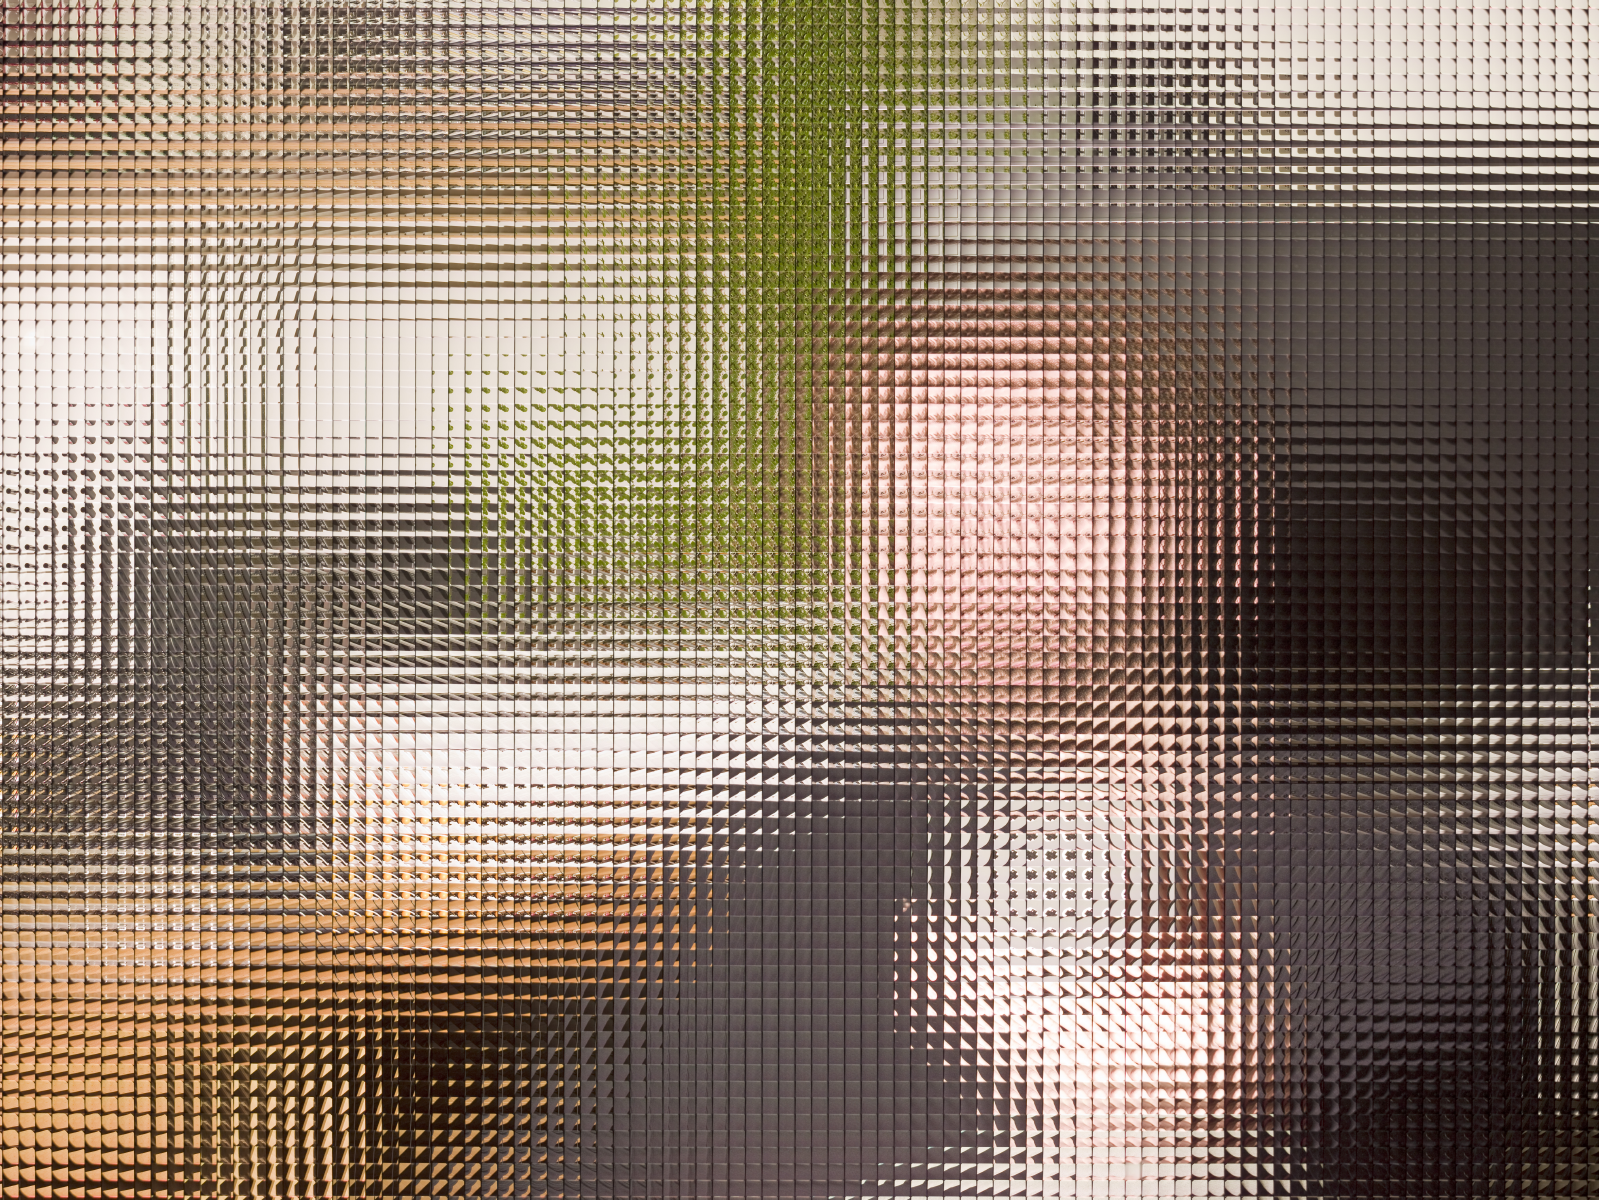
\includegraphics[angle=270,origin=b,width=0.35\textwidth]{472.eps}
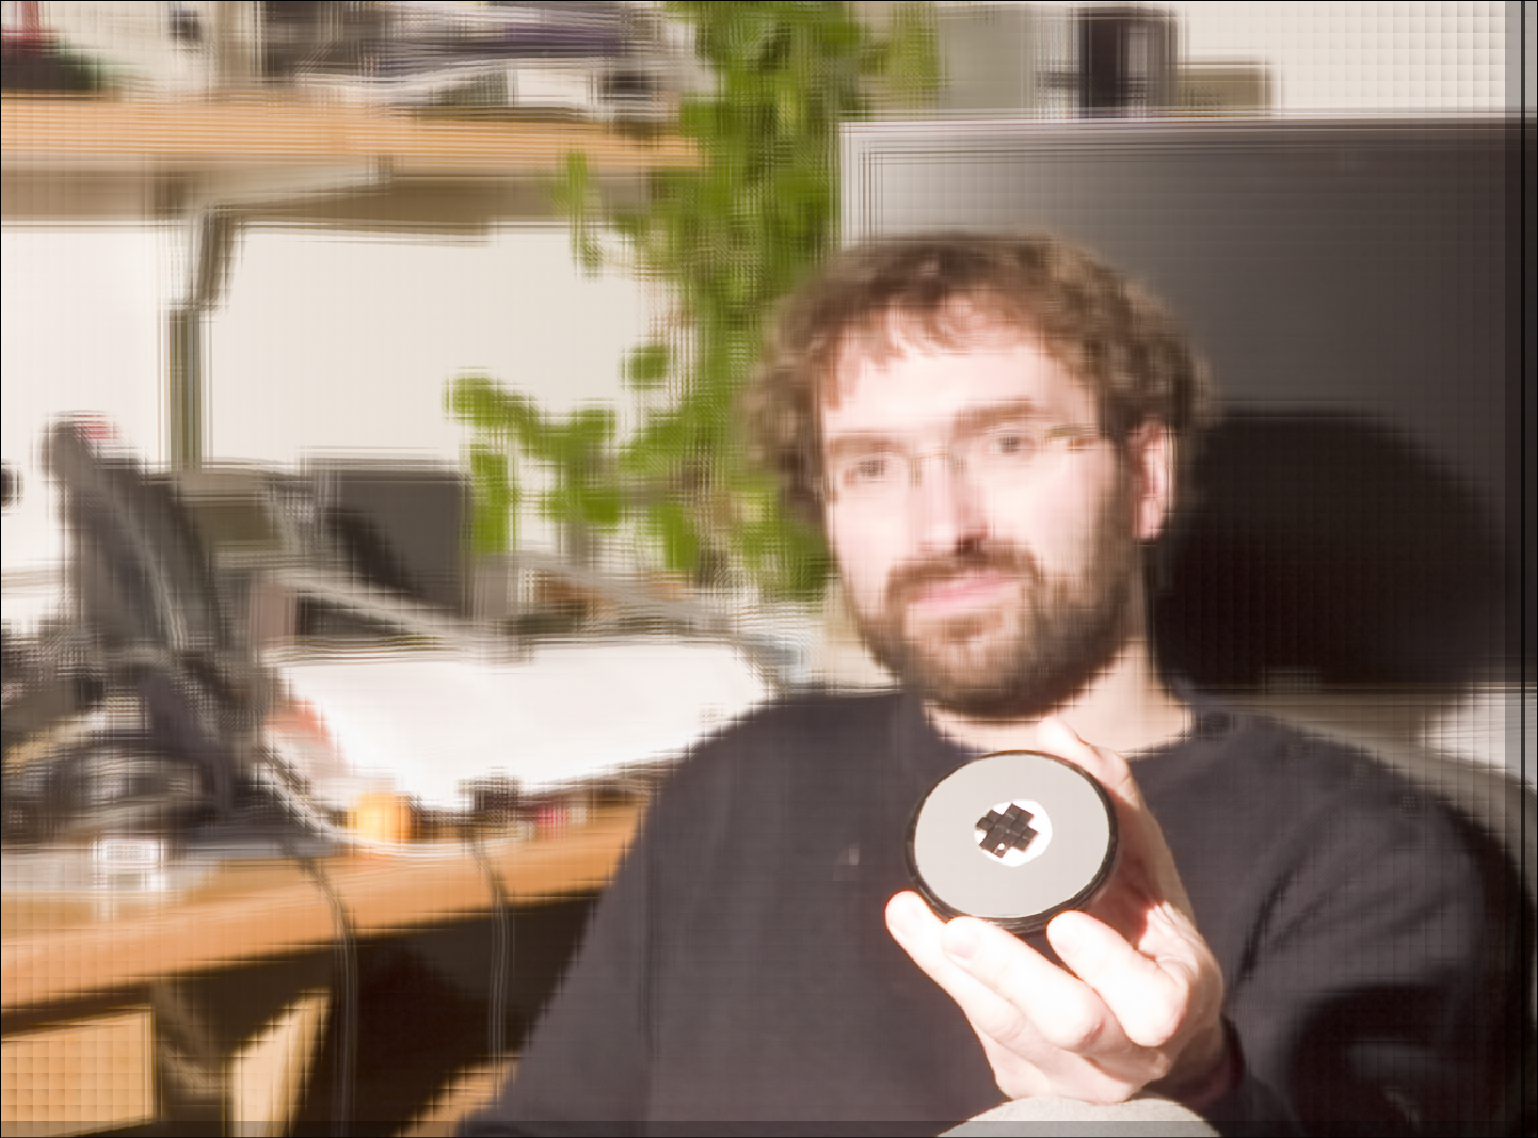
\includegraphics[angle=270,origin=b,width=0.35\textwidth]{gather.eps}
\caption{Gather}
\end{figure}

������7500x7500�饤�ȥե�����ɲ��������Υ�����󥰤Ǥ��롥��§Ū�ʥ��ƥ�
����׻��ǤϤʤ�����mapdist=0�Ǥ��롥

\begin{screen}
\tiny
\begin{verbatim}
orig()
{
  ry = (R+ofs)*IM;
  rx = (R+ofs);
  int w, pix, cvalR, cvalG, cvalB;

  for (row=PAD; row<OM-PAD; row++) {
    for (col=PAD; col<OM-PAD; col++) {
       c = ((row>>4)*R + (((~row&15)*ofs)>>4))*IM
          + (col>>4)*R + (((~col&15)*ofs)>>4);
      cvalR=0;
      cvalG=0;
      cvalB=0;
      for (i=-1; i<=1; i++) {
        for (j=-1; j<=1; j++) {
          Uint pix = in[c+ry*i+rx*j];
          w = weight[WBASE+i*MAXDELTA*2+j];
          cvalR += ((pix>>24)&255)*w;
          cvalG += ((pix>>16)&255)*w;
          cvalB += ((pix>> 8)&255)*w;
          count0++;
        }
      }
      out0[row*OM+col] = ((cvalR>>8)<<24) | ((cvalG>>8)<<16) | ((cvalB>>8)<<8);
} } }
\end{verbatim}
\end{screen}

\begin{screen}
\tiny
\begin{verbatim}
imax()
{
  Ull CHIP;
  ry = (R+ofs)*IM;
  rx = (R+ofs);
  int w, pix, cvalR, cvalG, cvalB;

  for (row=0; row<RRANGE; row++) { /* 0..381 */
    for (CHIP=0; CHIP<NCHIP; CHIP++) {
      for (col=0; col<CRANGE; col++) {
        for (oc=0; oc<OMAP; oc++) {
          c =((((CHIP*OMAP+oc)*RRANGE+row+PAD)>>4)*R + (((~((CHIP*OMAP+oc)*RRANGE+row+PAD)&15)*ofs)>>4))*IM
            + ((                      col+PAD)>>4)*R + (((~(                      col+PAD)&15)*ofs)>>4);
          /* 256  512 256 */
          pix = in[c+ry*(-1)+rx*(-1)]; w = 16; cvalR =((pix>>24)&255)*w; cvalG =((pix>>16)&255)*w; cvalB =((pix>> 8)&255)*w;
          pix = in[c+ry*(-1)+rx*( 0)]; w = 32; cvalR+=((pix>>24)&255)*w; cvalG+=((pix>>16)&255)*w; cvalB+=((pix>> 8)&255)*w;
          pix = in[c+ry*(-1)+rx*( 1)]; w = 16; cvalR+=((pix>>24)&255)*w; cvalG+=((pix>>16)&255)*w; cvalB+=((pix>> 8)&255)*w;
          /* 512 1024 512 */
          pix = in[c+ry*( 0)+rx*(-1)]; w = 32; cvalR+=((pix>>24)&255)*w; cvalG+=((pix>>16)&255)*w; cvalB+=((pix>> 8)&255)*w;
          pix = in[c+ry*( 0)+rx*( 0)]; w = 64; cvalR+=((pix>>24)&255)*w; cvalG+=((pix>>16)&255)*w; cvalB+=((pix>> 8)&255)*w;
          pix = in[c+ry*( 0)+rx*( 1)]; w = 32; cvalR+=((pix>>24)&255)*w; cvalG+=((pix>>16)&255)*w; cvalB+=((pix>> 8)&255)*w;
          /* 256  512 256 */
          pix = in[c+ry*( 1)+rx*(-1)]; w = 16; cvalR+=((pix>>24)&255)*w; cvalG+=((pix>>16)&255)*w; cvalB+=((pix>> 8)&255)*w;
          pix = in[c+ry*( 1)+rx*( 0)]; w = 32; cvalR+=((pix>>24)&255)*w; cvalG+=((pix>>16)&255)*w; cvalB+=((pix>> 8)&255)*w;
          pix = in[c+ry*( 1)+rx*( 1)]; w = 16; cvalR+=((pix>>24)&255)*w; cvalG+=((pix>>16)&255)*w; cvalB+=((pix>> 8)&255)*w;
          count1+=9;
          out1[((CHIP*OMAP+oc)*RRANGE+row+PAD)*OM+(col+PAD)] = ((cvalR>>8)<<24) | ((cvalG>>8)<<16) | ((cvalB>>8)<<8);
} } } } }
\end{verbatim}
\end{screen}

\begin{screen}
\tiny
\begin{verbatim}
imax()
{
  Ull  CHIP;  Ull  LOOP1, LOOP0;  Ull  INIT1, INIT0;
  Ull  AR[64][4];                     /* output of EX     in each unit */
  Ull  BR[64][4][4];                  /* output registers in each unit */
  Ull  r0, r1, r2, r3, r4, r5, r6, r7, r8, r9, r10, r11, r12, r13, r14, r15;
  Ull  r16, r17, r18, r19, r20, r21, r22, r23, r24, r25, r26, r27, r28, r29, r30, r31;
  Ull  c0, c1, c2, c3, ex0, ex1;  Ull  x[NCHIP];
  ry = (R+ofs)*IM;  rx = (R+ofs);
  Uint *ym_xm   = in         -ry-rx;
     :
  for (row=RRANGE-1; row>=0; row--) {
    int yin0[NCHIP];
    Uint *acci_ym0[NCHIP];    Uint *acci_yz0[NCHIP];    Uint *acci_yp0[NCHIP];
    Uint *acco_base0[NCHIP];  Uint *acco0[NCHIP];
         :
    Uint *acco_base5[NCHIP];  Uint *acco5[NCHIP];
    for (CHIP=0; CHIP<NCHIP; CHIP++) {
      int row0 = (CHIP*OMAP+0)*RRANGE+row+PAD;
      int yout0 = row0*OM;
      yin0[CHIP] = ((row0>>4)*R + (((~row0&15)*ofs)>>4))*IM;
      acci_ym0[CHIP] = in+yin0[CHIP]     -ry;      acci_yz0[CHIP] = in+yin0[CHIP];      acci_yp0[CHIP] = in+yin0[CHIP]     +ry;
      acco_base0[CHIP] = out1+yout0+PAD;  acco0[CHIP] = out1+yout0+PAD;
        :
      acco_base5[CHIP] = out1+yout5+PAD;  acco5[CHIP] = out1+yout5+PAD;
    }
//EMAX5A begin gather mapdist=0
    for (CHIP=0; CHIP<NCHIP; CHIP++) {
      for (INIT0=1,LOOP0=CRANGE,x[CHIP]=PAD-1; LOOP0--; INIT0=0) {
        exe(OP_ADD,  &x[CHIP], x[CHIP],  EXP_H3210,         1LL, EXP_H3210, 0LL, EXP_H3210, OP_NOP,   0LL, OP_NOP, 0LL);     /* stage#0 */
        exe(OP_SUB,  &r1,         -1LL,  EXP_H3210,     x[CHIP], EXP_H3210, 0LL, EXP_H3210, OP_AND,  15LL, OP_NOP, 0LL);     /* stage#1 */
        exe(OP_NOP,  &r2,      x[CHIP],  EXP_H3210,         0LL, EXP_H3210, 0LL, EXP_H3210, OP_OR,    0LL, OP_SRL, 4LL);     /* stage#1 */
        exe(OP_MLUH, &r3,           r1,  EXP_H3210,    (Ull)ofs, EXP_H3210, 0LL, EXP_H3210, OP_OR,    0LL, OP_SRL, 4LL);     /* stage#2 */
        exe(OP_MLUH, &r4,           r2,  EXP_H3210,        75LL, EXP_H3210, 0LL, EXP_H3210, OP_NOP,   0LL, OP_NOP, 0LL);     /* stage#2 */
        exe(OP_ADD3, &r0,           r3,  EXP_H3210,          r4, EXP_H3210,(Ull)yin0[CHIP], EXP_H3210,OP_OR,0LL,OP_SLL, 2LL);/* stage#3 */
        exe(OP_ADD,  &r1,           r3,  EXP_H3210,          r4, EXP_H3210, 0LL, EXP_H3210, OP_OR,    0LL, OP_NOP, 0LL);     /* stage#3 */
        mop(OP_LDWR,    1, &BR[4][0][1],  r0, (Ull)ym_xm, MSK_D0, (Ull)acci_ym0[CHIP], IM, 0, 0, (Ull)NULL, IM);         /* stage#4 */
        mop(OP_LDWR,    1, &BR[4][1][1],  r0, (Ull)ym_xz, MSK_D0, (Ull)acci_ym0[CHIP], IM, 0, 0, (Ull)NULL, IM);         /* stage#4 */
        mop(OP_LDWR,    1, &BR[4][2][1],  r0, (Ull)ym_xp, MSK_D0, (Ull)acci_ym0[CHIP], IM, 0, 0, (Ull)NULL, IM);         /* stage#4 */
        exe(OP_MLUH,  &r10,     BR[4][0][1],  EXP_B5410,        16LL, EXP_H3210, 0LL, EXP_H3210, OP_NOP,  0LL, OP_NOP, 0LL); /* stage#5 */
        exe(OP_MLUH,  &r11,     BR[4][1][1],  EXP_B5410,        32LL, EXP_H3210, 0LL, EXP_H3210, OP_NOP,  0LL, OP_NOP, 0LL); /* stage#5 */
        exe(OP_MLUH,  &r12,     BR[4][2][1],  EXP_B5410,        16LL, EXP_H3210, 0LL, EXP_H3210, OP_NOP,  0LL, OP_NOP, 0LL); /* stage#5 */
        exe(OP_MLUH,  &r13,     BR[4][0][1],  EXP_B7632,        16LL, EXP_H3210, 0LL, EXP_H3210, OP_NOP,  0LL, OP_NOP, 0LL); /* stage#6 */
        exe(OP_MLUH,  &r14,     BR[4][1][1],  EXP_B7632,        32LL, EXP_H3210, 0LL, EXP_H3210, OP_NOP,  0LL, OP_NOP, 0LL); /* stage#6 */
        exe(OP_MLUH,  &r15,     BR[4][2][1],  EXP_B7632,        16LL, EXP_H3210, 0LL, EXP_H3210, OP_NOP,  0LL, OP_NOP, 0LL); /* stage#6 */
        exe(OP_MAUH3, &r20,  r10, EXP_H3210,  r11, EXP_H3210,  r12, EXP_H3210, OP_NOP, 0LL, OP_NOP, 0LL);                    /* stage#6 */
        mop(OP_LDWR,    1, &BR[6][0][1], r0, (Ull)yz_xm, MSK_D0, (Ull)acci_yz0[CHIP], IM, 0, 0, (Ull)NULL, IM);          /* stage#6 */
        mop(OP_LDWR,    1, &BR[6][1][1], r0, (Ull)yz_xz, MSK_D0, (Ull)acci_yz0[CHIP], IM, 0, 0, (Ull)NULL, IM);          /* stage#6 */
        mop(OP_LDWR,    1, &BR[6][2][1], r0, (Ull)yz_xp, MSK_D0, (Ull)acci_yz0[CHIP], IM, 0, 0, (Ull)NULL, IM);          /* stage#6 */
        exe(OP_MAUH3, &r21,  r13, EXP_H3210,  r14, EXP_H3210,  r15, EXP_H3210, OP_NOP, 0LL, OP_NOP, 0LL);                    /* stage#7 */
        exe(OP_MLUH,  &r10,     BR[6][0][1],  EXP_B5410,        32LL, EXP_H3210, 0LL, EXP_H3210, OP_NOP,  0LL, OP_NOP, 0LL); /* stage#7 */
        exe(OP_MLUH,  &r11,     BR[6][1][1],  EXP_B5410,        64LL, EXP_H3210, 0LL, EXP_H3210, OP_NOP,  0LL, OP_NOP, 0LL); /* stage#7 */
        exe(OP_MLUH,  &r12,     BR[6][2][1],  EXP_B5410,        32LL, EXP_H3210, 0LL, EXP_H3210, OP_NOP,  0LL, OP_NOP, 0LL); /* stage#7 */
        exe(OP_MLUH,  &r13,     BR[6][0][1],  EXP_B7632,        32LL, EXP_H3210, 0LL, EXP_H3210, OP_NOP,  0LL, OP_NOP, 0LL); /* stage#8 */
        exe(OP_MLUH,  &r14,     BR[6][1][1],  EXP_B7632,        64LL, EXP_H3210, 0LL, EXP_H3210, OP_NOP,  0LL, OP_NOP, 0LL); /* stage#8 */
        exe(OP_MLUH,  &r15,     BR[6][2][1],  EXP_B7632,        32LL, EXP_H3210, 0LL, EXP_H3210, OP_NOP,  0LL, OP_NOP, 0LL); /* stage#8 */
        exe(OP_MAUH3, &r22,  r10, EXP_H3210,  r11, EXP_H3210,  r12, EXP_H3210, OP_NOP, 0LL, OP_NOP, 0LL);                    /* stage#8 */
        mop(OP_LDWR,    1, &BR[8][0][1], r0, (Ull)yp_xm, MSK_D0, (Ull)acci_yp0[CHIP], IM, 0, 0, (Ull)NULL, IM);          /* stage#8 */
        mop(OP_LDWR,    1, &BR[8][1][1], r0, (Ull)yp_xz, MSK_D0, (Ull)acci_yp0[CHIP], IM, 0, 0, (Ull)NULL, IM);          /* stage#8 */
        mop(OP_LDWR,    1, &BR[8][2][1], r0, (Ull)yp_xp, MSK_D0, (Ull)acci_yp0[CHIP], IM, 0, 0, (Ull)NULL, IM);          /* stage#8 */
        exe(OP_MAUH3, &r23,  r13, EXP_H3210,  r14, EXP_H3210,  r15, EXP_H3210, OP_NOP, 0LL, OP_NOP, 0LL);                    /* stage#9 */
        exe(OP_MLUH,  &r10,     BR[8][0][1],  EXP_B5410,        16LL, EXP_H3210, 0LL, EXP_H3210, OP_NOP,  0LL, OP_NOP, 0LL); /* stage#9 */
        exe(OP_MLUH,  &r11,     BR[8][1][1],  EXP_B5410,        32LL, EXP_H3210, 0LL, EXP_H3210, OP_NOP,  0LL, OP_NOP, 0LL); /* stage#9 */
        exe(OP_MLUH,  &r12,     BR[8][2][1],  EXP_B5410,        16LL, EXP_H3210, 0LL, EXP_H3210, OP_NOP,  0LL, OP_NOP, 0LL); /* stage#9 */
        exe(OP_MLUH,  &r13,     BR[8][0][1],  EXP_B7632,        16LL, EXP_H3210, 0LL, EXP_H3210, OP_NOP,  0LL, OP_NOP, 0LL); /* stage#10 */
        exe(OP_MLUH,  &r14,     BR[8][1][1],  EXP_B7632,        32LL, EXP_H3210, 0LL, EXP_H3210, OP_NOP,  0LL, OP_NOP, 0LL); /* stage#10 */
        exe(OP_MLUH,  &r15,     BR[8][2][1],  EXP_B7632,        16LL, EXP_H3210, 0LL, EXP_H3210, OP_NOP,  0LL, OP_NOP, 0LL); /* stage#10 */
        exe(OP_MAUH3, &r24,  r10, EXP_H3210,  r11, EXP_H3210,  r12, EXP_H3210, OP_NOP, 0LL, OP_NOP, 0LL);                    /* stage#10 */
        exe(OP_MAUH3, &r25,  r13, EXP_H3210,  r14, EXP_H3210,  r15, EXP_H3210, OP_NOP, 0LL, OP_NOP, 0LL);                    /* stage#11 */
        exe(OP_MAUH3, &r30,  r20, EXP_H3210,  r22, EXP_H3210,  r24, EXP_H3210, OP_AND, -1LL, OP_SRLM, 8LL);                  /* stage#12 */
        exe(OP_MAUH3, &r31,  r21, EXP_H3210,  r23, EXP_H3210,  r25, EXP_H3210, OP_AND, -1LL, OP_SRLM, 8LL);                  /* stage#12 */
        exe(OP_MH2BW, &r29,  r31, EXP_H3210,  r30, EXP_H3210,  0LL, EXP_H3210, OP_NOP,  0LL, OP_NOP, 0LL);                   /* stage#13 */
        mop(OP_STWR,    3, &r29, (Ull)(acco0[CHIP]++), 0LL, MSK_D0, (Ull)acco_base0[CHIP], CRANGE, 0,0,(Ull)NULL,CRANGE);/* stage#13 */
        :
        /**********************/
        exe(OP_ADD,  &r0,           r1,  EXP_H3210,   (Ull)yin5[CHIP], EXP_H3210, 0LL, EXP_H3210, OP_OR,   0LL, OP_SLL, 2LL); /* stage#53 */
        /**********************/
        mop(OP_LDWR,    1, &BR[54][0][1],  r0, (Ull)ym_xm, MSK_D0, (Ull)acci_ym5[CHIP], IM, 0, 0, (Ull)NULL, IM);         /* stage#54 */
        mop(OP_LDWR,    1, &BR[54][1][1],  r0, (Ull)ym_xz, MSK_D0, (Ull)acci_ym5[CHIP], IM, 0, 0, (Ull)NULL, IM);         /* stage#54 */
        mop(OP_LDWR,    1, &BR[54][2][1],  r0, (Ull)ym_xp, MSK_D0, (Ull)acci_ym5[CHIP], IM, 0, 0, (Ull)NULL, IM);         /* stage#54 */
        exe(OP_MLUH,  &r10,     BR[54][0][1],  EXP_B5410,        16LL, EXP_H3210, 0LL, EXP_H3210, OP_NOP,  0LL, OP_NOP, 0LL); /* stage#55 */
        exe(OP_MLUH,  &r11,     BR[54][1][1],  EXP_B5410,        32LL, EXP_H3210, 0LL, EXP_H3210, OP_NOP,  0LL, OP_NOP, 0LL); /* stage#55 */
        exe(OP_MLUH,  &r12,     BR[54][2][1],  EXP_B5410,        16LL, EXP_H3210, 0LL, EXP_H3210, OP_NOP,  0LL, OP_NOP, 0LL); /* stage#55 */
        exe(OP_MLUH,  &r13,     BR[54][0][1],  EXP_B7632,        16LL, EXP_H3210, 0LL, EXP_H3210, OP_NOP,  0LL, OP_NOP, 0LL); /* stage#56 */
        exe(OP_MLUH,  &r14,     BR[54][1][1],  EXP_B7632,        32LL, EXP_H3210, 0LL, EXP_H3210, OP_NOP,  0LL, OP_NOP, 0LL); /* stage#56 */
        exe(OP_MLUH,  &r15,     BR[54][2][1],  EXP_B7632,        16LL, EXP_H3210, 0LL, EXP_H3210, OP_NOP,  0LL, OP_NOP, 0LL); /* stage#56 */
        exe(OP_MAUH3, &r20,  r10, EXP_H3210,  r11, EXP_H3210,  r12, EXP_H3210, OP_NOP, 0LL, OP_NOP, 0LL);                     /* stage#56 */
        mop(OP_LDWR,    1, &BR[56][0][1], r0, (Ull)yz_xm, MSK_D0, (Ull)acci_yz5[CHIP], IM, 0, 0, (Ull)NULL, IM);          /* stage#56 */
        mop(OP_LDWR,    1, &BR[56][1][1], r0, (Ull)yz_xz, MSK_D0, (Ull)acci_yz5[CHIP], IM, 0, 0, (Ull)NULL, IM);          /* stage#56 */
        mop(OP_LDWR,    1, &BR[56][2][1], r0, (Ull)yz_xp, MSK_D0, (Ull)acci_yz5[CHIP], IM, 0, 0, (Ull)NULL, IM);          /* stage#56 */
        exe(OP_MAUH3, &r21,  r13, EXP_H3210,  r14, EXP_H3210,  r15, EXP_H3210, OP_NOP, 0LL, OP_NOP, 0LL);                     /* stage#57 */
        exe(OP_MLUH,  &r10,     BR[56][0][1],  EXP_B5410,        32LL, EXP_H3210, 0LL, EXP_H3210, OP_NOP,  0LL, OP_NOP, 0LL); /* stage#57 */
        exe(OP_MLUH,  &r11,     BR[56][1][1],  EXP_B5410,        64LL, EXP_H3210, 0LL, EXP_H3210, OP_NOP,  0LL, OP_NOP, 0LL); /* stage#57 */
        exe(OP_MLUH,  &r12,     BR[56][2][1],  EXP_B5410,        32LL, EXP_H3210, 0LL, EXP_H3210, OP_NOP,  0LL, OP_NOP, 0LL); /* stage#57 */
        exe(OP_MLUH,  &r13,     BR[56][0][1],  EXP_B7632,        32LL, EXP_H3210, 0LL, EXP_H3210, OP_NOP,  0LL, OP_NOP, 0LL); /* stage#58 */
        exe(OP_MLUH,  &r14,     BR[56][1][1],  EXP_B7632,        64LL, EXP_H3210, 0LL, EXP_H3210, OP_NOP,  0LL, OP_NOP, 0LL); /* stage#58 */
        exe(OP_MLUH,  &r15,     BR[56][2][1],  EXP_B7632,        32LL, EXP_H3210, 0LL, EXP_H3210, OP_NOP,  0LL, OP_NOP, 0LL); /* stage#58 */
        exe(OP_MAUH3, &r22,  r10, EXP_H3210,  r11, EXP_H3210,  r12, EXP_H3210, OP_NOP, 0LL, OP_NOP, 0LL);                     /* stage#58 */
        mop(OP_LDWR,    1, &BR[58][0][1], r0, (Ull)yp_xm, MSK_D0, (Ull)acci_yp5[CHIP], IM, 0, 0, (Ull)NULL, IM);          /* stage#58 */
        mop(OP_LDWR,    1, &BR[58][1][1], r0, (Ull)yp_xz, MSK_D0, (Ull)acci_yp5[CHIP], IM, 0, 0, (Ull)NULL, IM);          /* stage#58 */
        mop(OP_LDWR,    1, &BR[58][2][1], r0, (Ull)yp_xp, MSK_D0, (Ull)acci_yp5[CHIP], IM, 0, 0, (Ull)NULL, IM);          /* stage#58 */
        exe(OP_MAUH3, &r23,  r13, EXP_H3210,  r14, EXP_H3210,  r15, EXP_H3210, OP_NOP, 0LL, OP_NOP, 0LL);                     /* stage#59 */
        exe(OP_MLUH,  &r10,     BR[58][0][1],  EXP_B5410,        16LL, EXP_H3210, 0LL, EXP_H3210, OP_NOP,  0LL, OP_NOP, 0LL); /* stage#59 */
        exe(OP_MLUH,  &r11,     BR[58][1][1],  EXP_B5410,        32LL, EXP_H3210, 0LL, EXP_H3210, OP_NOP,  0LL, OP_NOP, 0LL); /* stage#59 */
        exe(OP_MLUH,  &r12,     BR[58][2][1],  EXP_B5410,        16LL, EXP_H3210, 0LL, EXP_H3210, OP_NOP,  0LL, OP_NOP, 0LL); /* stage#59 */
        exe(OP_MLUH,  &r13,     BR[58][0][1],  EXP_B7632,        16LL, EXP_H3210, 0LL, EXP_H3210, OP_NOP,  0LL, OP_NOP, 0LL); /* stage#60 */
        exe(OP_MLUH,  &r14,     BR[58][1][1],  EXP_B7632,        32LL, EXP_H3210, 0LL, EXP_H3210, OP_NOP,  0LL, OP_NOP, 0LL); /* stage#60 */
        exe(OP_MLUH,  &r15,     BR[58][2][1],  EXP_B7632,        16LL, EXP_H3210, 0LL, EXP_H3210, OP_NOP,  0LL, OP_NOP, 0LL); /* stage#60 */
        exe(OP_MAUH3, &r24,  r10, EXP_H3210,  r11, EXP_H3210,  r12, EXP_H3210, OP_NOP, 0LL, OP_NOP, 0LL);                     /* stage#60 */
        exe(OP_MAUH3, &r25,  r13, EXP_H3210,  r14, EXP_H3210,  r15, EXP_H3210, OP_NOP, 0LL, OP_NOP, 0LL);                     /* stage#61 */
        exe(OP_MAUH3, &r30,  r20, EXP_H3210,  r22, EXP_H3210,  r24, EXP_H3210, OP_AND, -1LL, OP_SRLM, 8LL); /* stage#62 */
        exe(OP_MAUH3, &r31,  r21, EXP_H3210,  r23, EXP_H3210,  r25, EXP_H3210, OP_AND, -1LL, OP_SRLM, 8LL); /* stage#62 */
        exe(OP_MH2BW, &r29,  r31, EXP_H3210,  r30, EXP_H3210,  0LL, EXP_H3210, OP_NOP,  0LL, OP_NOP, 0LL);  /* stage#63 */
        mop(OP_STWR,    3, &r29, (Ull)(acco5[CHIP]++), 0LL, MSK_D0, (Ull)acco_base5[CHIP], CRANGE, 0,0,(Ull)NULL, CRANGE);/* stage#63 */
    } }
//EMAX5A end
  }
//EMAX5A drain_dirty_lmm
}
\end{verbatim}
\end{screen}

\begin{figure}[htbp]
\center
\epsfile{file=gather+rmm-gather-emax6.eps,width=1.00\textwidth}
\caption{Lightfield�������}
\end{figure}

\clearpage

\subsection{Lightfield����������}

\shabox{
\leftline{cent\% make -f Makefile-csim.emax6+dma gdepth-csim.emax6+dma clean}
\leftline{cent\% ../../src/csim/csim -x gdepth-csim.emax6+dma}
}

\shabox{
\leftline{zynq\% make -f Makefile-zynq.emax6+dma gdepth-zynq.emax6+dma clean}
\leftline{zynq\% ./gdepth-zynq.emax6+dma}
}

\begin{figure}[htbp]
\center
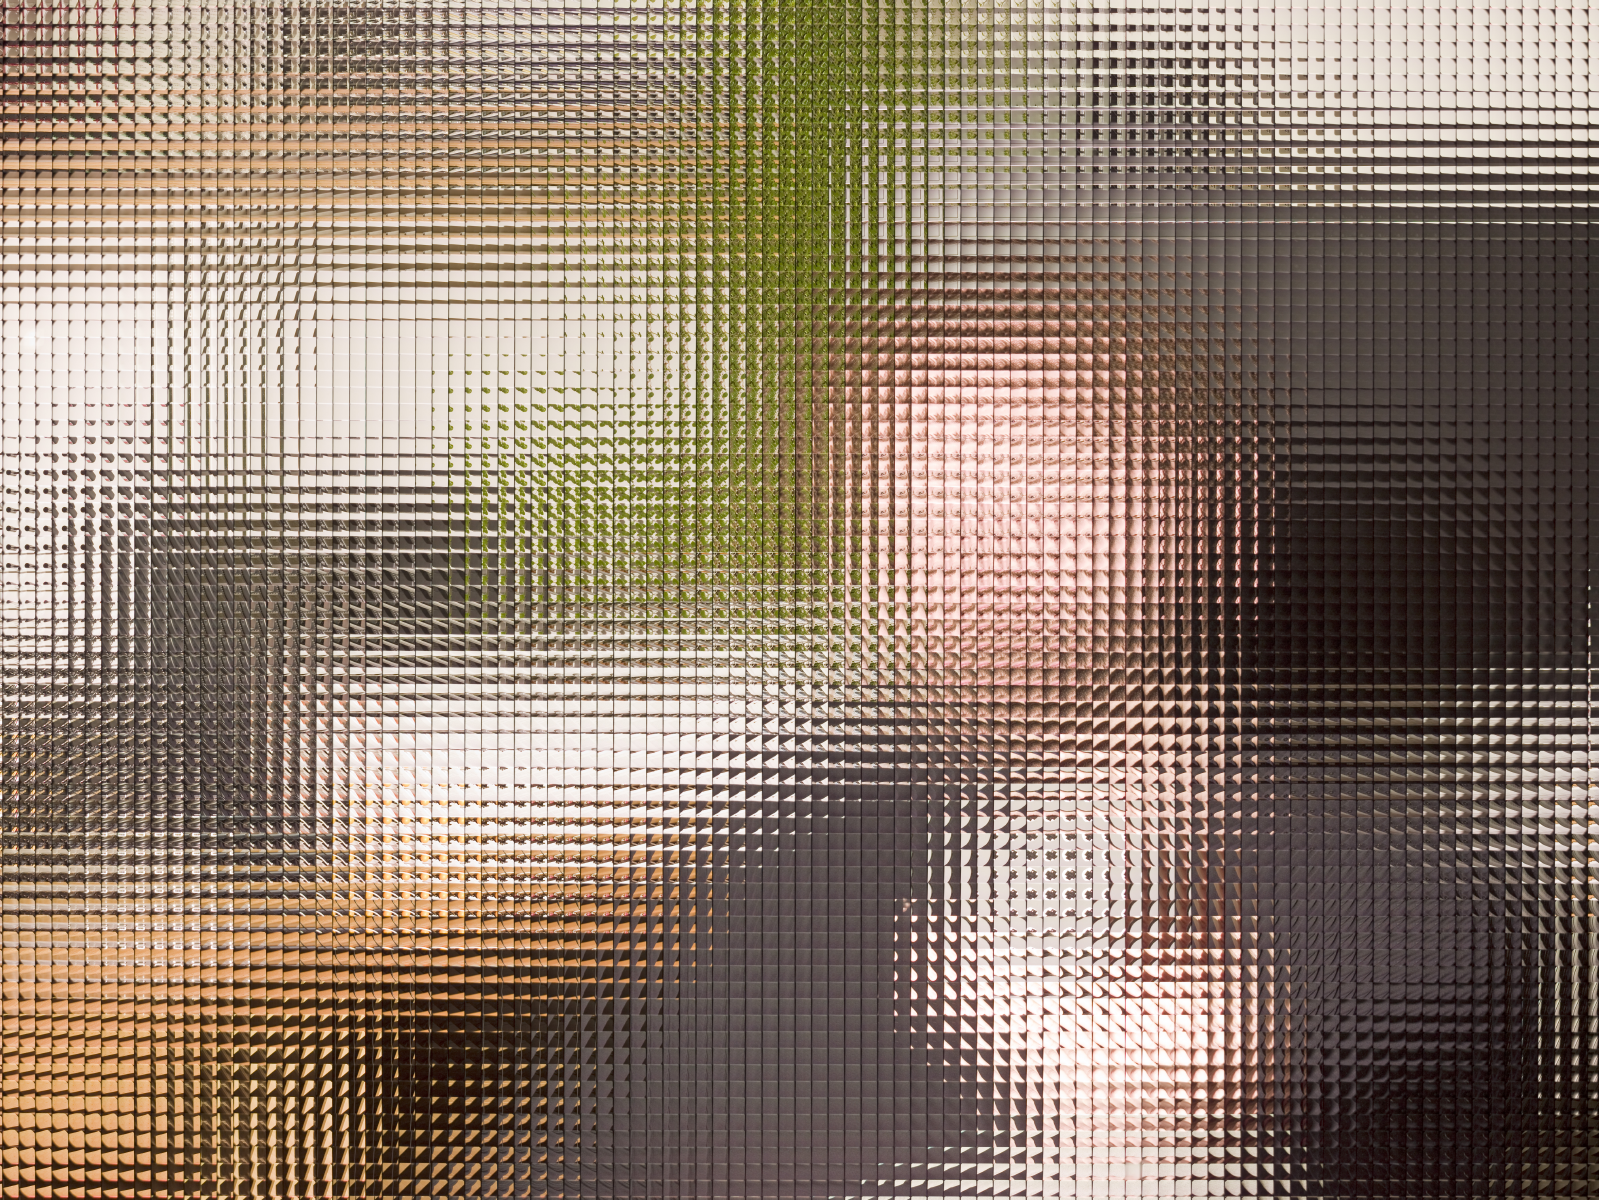
\includegraphics[angle=270,origin=b,width=0.35\textwidth]{472.eps}
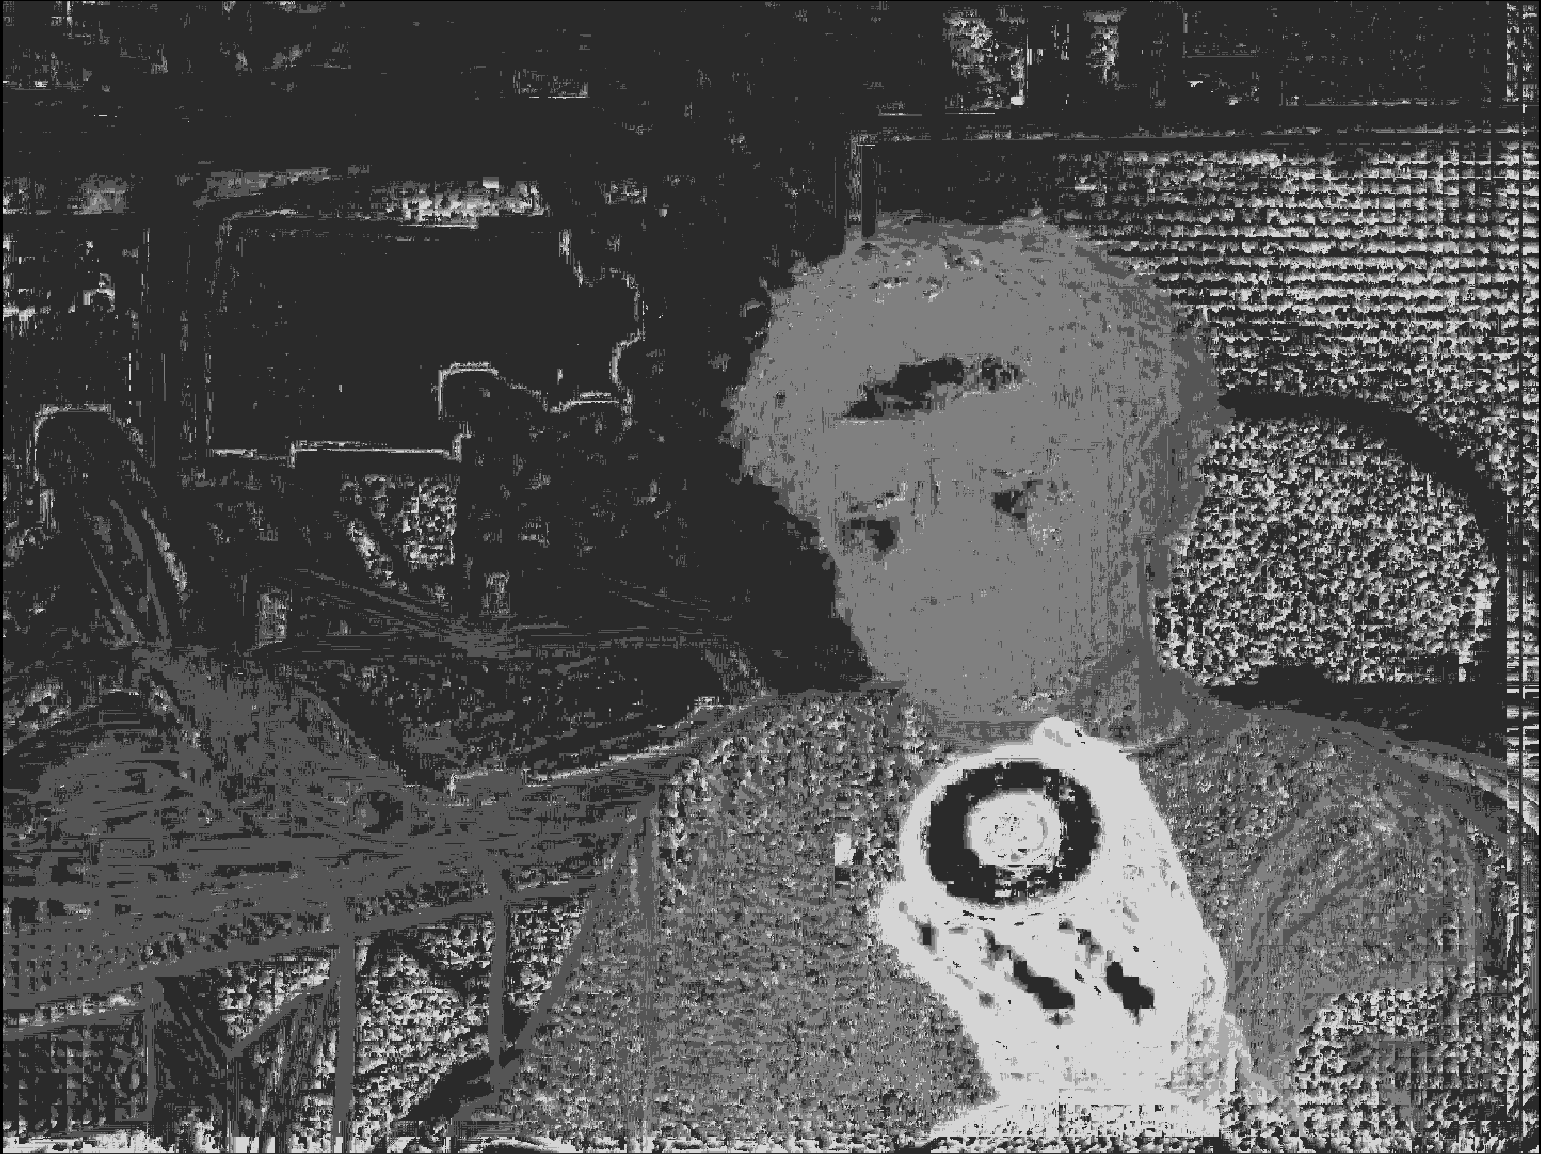
\includegraphics[angle=270,origin=b,width=0.35\textwidth]{gdepth.eps}
\caption{Gdepth}
\end{figure}

\begin{figure}[htbp]
\center
\includegraphics[width=0.80\textwidth]{lf0.eps}
\caption{\label{fig:lf0}Lightfield}
\end{figure}

������7500x7500�饤�ȥե�����ɲ��������ε�Υ���������Ǥ��롥��§Ū�ʥ��ƥ�
����׻��ǤϤʤ���Τ�Ŭ��Ūmapdist����Ѥ��Ƥ��ꡤɸ���ͤ�mapdist=3�Ǥ��롥
��\ref{fig:lf0}(a)�ˡ�LF�Υǡ�����¤��(b)�˳�unit��Sum of absolute
difference��SAD�˱黻���1��������12x4������CGRA�򼨤���(b)�Ͽ�
\ref{fig:cnn0}��Ʊ�͡��ǡ����ե�������դ򼨤��Ƥ��롥75x75���ǤΥޥ�������
�󥺲�����100x100�γʻ���������֤��졤���Τ�7500x7500���Ǥβ�����in�ˤ�����
���Ȳ��ꤹ�롥�ƥޥ����������ʾ岼������ȿž�ˤΰ�����3x3�ˤˤĤ��ơ�
75+ofs����Υ�줿ʣ���Υޥ����������֤�SAD���ᡤ�Ǿ��Ȥʤ�ofs���Υ����
��out�ˤȤ����������롥����Ū�ˤϡ������p0�ˤ�3x3�����Τ���6���Ǥȡ�����6��
���p1�ˤ�3x3�����Τ���6���Ǥ��Ф���SAD���ᡤ���36���Ǥ�SAD���߻����Ƥ��롥
CGRA����Ƭ�ʡ�unit[0][*]�ˤˡ�y$\#$0�ΰ��֤ˤ�����3x3���ǤκǾ�ԡ�i$\#$-1��
�б��ˤ������ơ�1��ʬ�β�������¸������ƬLMM����6�ս��Υ��Ū�����ɡ�p0��
p1��ޤ�ˤ�Ԥ������������ʬ�ˡ���2�ʡ�unit[1][*]�ˤ���3�ʡ�unit[2][*]�ˤϡ�
�ơ���y$\#$-1�����y$\#$1�ΰ��֡�p1�ˤ���Υ����ɤ�Ԥ�����Ƭ�ʤˤƼ�������
p0����Ӥ��롥CGRA��9���̲ᤷ����ˡ������2�ʤ��Ѥ��ơ�4���SAD��1�Ĥ�SAD��
�߻����롥�dz��롼�פˤ�����ofs���ѹ��������κǾ�sad����¸���Ƥ�������꾮
����SAD�ͤ�����줿���ˡ�����դ����ȥ����Ѥ���sad��out�򹹿����롥���Τ�
���ˡ�36���Ǥ�SAD�ͤ���뤿���11�ʤ���Ѥ���44����40�Ĥα黻�郎�����ƥ�
�֤Ȥʤ롥���Τ��ʿ��ϡ�(b)�˼��������ȥ�1�ʤ�ޤ�12�ʤˡ�c�Υ��ɥ쥹�׻���
��ɬ�פ�6�ʤ����֤������18�ʤȤʤ롥(c)�Ϥ���ˡ����̤�N���åפ�ʬ�䤷����
�ϲ�����������������ƥ��åפ�36���Ǥ�SAD�黻��REP�ȼ����Ǥ����ʿ����������
��μ����Ǥ��롥�ʤ�ofs�򹹿�����dz��롼�פϾ�ά���Ƥ��롥�ʾ�α黻���פ�
������Ū����������ϡ�CGRA��ư�����ٱ��REP$\ge$2�ξ��14xREP+3��������ˤ�
���LMM�����촹�����֤�����ȡ�ofs������40xOM$^2$/(REPxN)�Ȥʤ롥out��1����
�������뤿���p0����6���ǡ�p1����36����ɬ�פǤ����ΤΡ�p0��p1�ο�ʿ������
�ȤϽ�ʣ�ȹͤ���ȡ�����ŪDDR-LMM��ž���̤ϡ�in:9xOM$^2$ + out:OM$^2$�Ǥ���
�����ϲ������Τ�IM$^2$�Ǥ��뤬in�Ȥ��ƻ��Ȥ����̤�9xOM$^2$�ˡ�

\begin{screen}
\tiny
\begin{verbatim}
orig()
{
  ry = (R+ofs)*IM;
  rx = (R+ofs); /* ofs: from 8 to 14 */
  for (row=PAD; row<OM-PAD; row++) {
    for (col=PAD; col<OM-PAD; col++) {
      c =((row>>4)*R + (((~row&15)*ofs)>>4))*IM
        + (col>>4)*R + (((~col&15)*ofs)>>4);
      s = 0;
      for (y=-1; y<=1; y++) {
        for (x=-1; x<=1; x++) {
          if (x == 0) continue;
          for (i=-1; i<=1; i++) {
            for (j=-1; j<=1; j++) {
              if (j == 0) continue;
              p0 = in[c     +(i*IM)     +j]; /* center */
              p1 = in[c+ry*y+(i*IM)+rx*x+j]; /* comparand */
              s += dif(p0, p1);
              if (s > 0xffff) s = 0xffff;
              count0++;
      } } } }
      if (sad0[row*OM+col]>TH && s<sad0[row*OM+col]) {
        sad0[row*OM+col] = s;
        out0[row*OM+col] = ofs;
} } } }
\end{verbatim}
\end{screen}

\begin{screen}
\tiny
\begin{verbatim}
imax()
{
  Ull CHIP;
  ry = (R+ofs)*IM;
  rx = (R+ofs); /* ofs: from 8 to 14 */
  for (row=0; row<RRANGE; row++) { /* 0..381 */
    for (CHIP=0; CHIP<NCHIP; CHIP++) {
      for (col=0; col<CRANGE; col++) {
        for (oc=0; oc<OMAP; oc++) {
          c =((((CHIP*OMAP+oc)*RRANGE+row+PAD)>>4)*R + (((~((CHIP*OMAP+oc)*RRANGE+row+PAD)&15)*ofs)>>4))*IM
            + ((                      col+PAD)>>4)*R + (((~(                      col+PAD)&15)*ofs)>>4);
          s = 0;
          for (y=-1; y<=1; y++) {
            for (x=-1; x<=1; x++) {
              if (x == 0) continue;
              for (i=-1; i<=1; i++) {
                for (j=-1; j<=1; j++) {
                  if (j == 0) continue;
                  p0 = in[c     +(i*IM)     +j]; /* center */
                  p1 = in[c+ry*y+(i*IM)+rx*x+j]; /* comparand */
                  s += dif(p0, p1);
                  count1++;
          } } } }
          if (sad1[((CHIP*OMAP+oc)*RRANGE+row+PAD)*OM+(col)+PAD]>TH && s<sad1[((CHIP*OMAP+oc)*RRANGE+row+PAD)*OM+(col+PAD)]) {
            sad1[((CHIP*OMAP+oc)*RRANGE+row+PAD)*OM+(col+PAD)] = s;
            out1[((CHIP*OMAP+oc)*RRANGE+row+PAD)*OM+(col+PAD)] = ofs;
} } } } } }
\end{verbatim}
\end{screen}

\begin{screen}
\tiny
\begin{verbatim}
imax()
{
  Ull  CHIP;  Ull  LOOP1, LOOP0;  Ull  INIT1, INIT0;
  Ull  AR[64][4];                     /* output of EX     in each unit */
  Ull  BR[64][4][4];                  /* output registers in each unit */
  Ull  r0, r1, r2, r3, r4, r5, r6, r7, r8, r9, r10, r11, r12, r13, r14, r15;
  Ull  r16, r17, r18, r19, r20, r21, r22, r23, r24, r25, r26, r27, r28, r29, r30, r31;
  Ull  c0, c1, c2, c3, ex0, ex1;  Ull  x[NCHIP];
  ry = (R+ofs)*IM; rx = (R+ofs);
  Uint *yzm_xm_m4 = in-IM   -rx-1;  Uint *yzm_xm_p4 = in-IM   -rx+1;
    :
  Uint *ypp_xp_m4 = in+IM+ry+rx-1;  Uint *ypp_xp_p4 = in+IM+ry+rx+1;
  for (row=RRANGE-1; row>=0; row--) {
    int  yin0[NCHIP];
    Uint *acci_yzm0[NCHIP];  Uint *acci_ymm0[NCHIP];  Uint *acci_ypm0[NCHIP];
    Uint *acci_yzz0[NCHIP];  Uint *acci_ymz0[NCHIP];  Uint *acci_ypz0[NCHIP];
    Uint *acci_yzp0[NCHIP];  Uint *acci_ymp0[NCHIP];  Uint *acci_ypp0[NCHIP];
    Uint *sadx_base0[NCHIP]; Uint *sadi0[NCHIP]; Uint *sado0[NCHIP];
    Uint *acco_base0[NCHIP]; Uint *acco0[NCHIP];
      :
    Uint *sadi_base0[NCHIP];  Uint *sadi0[NCHIP]; Uint *sado_base0[NCHIP];  Uint *sado0[NCHIP]; Uint *acco_base0[NCHIP];  Uint *acco0[NCHIP];
      :
    for (CHIP=0; CHIP<NCHIP; CHIP++) {
      yin0[CHIP] = ((row0>>4)*R + (((~row0&15)*ofs)>>4))*IM;
      acci_yzm0[CHIP] = in+yin0[CHIP]-IM;  acci_ymm0[CHIP] = in+yin0[CHIP]-IM-ry;  acci_ypm0[CHIP] = in+yin0[CHIP]-IM+ry;
      acci_yzz0[CHIP] = in+yin0[CHIP];     acci_ymz0[CHIP] = in+yin0[CHIP]   -ry;  acci_ypz0[CHIP] = in+yin0[CHIP]   +ry;
      acci_yzp0[CHIP] = in+yin0[CHIP]+IM;  acci_ymp0[CHIP] = in+yin0[CHIP]+IM-ry;  acci_ypp0[CHIP] = in+yin0[CHIP]+IM+ry;
      sadx_base0[CHIP] = sad1+yout0+PAD;  sadi0[CHIP] = sad1+yout0+PAD;  sado0[CHIP] = sad1+yout0+PAD;
      acco_base0[CHIP] = out1+yout0+PAD;  acco0[CHIP] = out1+yout0+PAD;
        :
    }
//EMAX5A begin gdepth mapdist=3
    for (CHIP=0; CHIP<NCHIP; CHIP++) {
      for (INIT0=1,LOOP0=CRANGE,x[CHIP]=PAD-1; LOOP0--; INIT0=0) {
        exe(OP_ADD,  &x[CHIP], x[CHIP],  EXP_H3210,        1LL, EXP_H3210, 0LL, EXP_H3210, OP_NOP,   0LL, OP_NOP, 0LL);   /* stage#0 */
        exe(OP_SUB,  &r1,         -1LL,  EXP_H3210,    x[CHIP], EXP_H3210, 0LL, EXP_H3210, OP_AND,  15LL, OP_NOP, 0LL);   /* stage#1 */
        exe(OP_NOP,  &r2,      x[CHIP],  EXP_H3210,        0LL, EXP_H3210, 0LL, EXP_H3210, OP_OR,    0LL, OP_SRL, 4LL);   /* stage#1 */
        exe(OP_MLUH, &r3,           r1,  EXP_H3210,   (Ull)ofs, EXP_H3210, 0LL, EXP_H3210, OP_OR,    0LL, OP_SRL, 4LL);   /* stage#2 */
        exe(OP_MLUH, &r4,           r2,  EXP_H3210,       75LL, EXP_H3210, 0LL, EXP_H3210, OP_NOP,   0LL, OP_NOP, 0LL);   /* stage#2 */
        exe(OP_ADD3, &r0,           r3,  EXP_H3210,         r4, EXP_H3210,(Ull)yin0[CHIP],EXP_H3210,OP_OR,0LL,OP_SLL,2LL);/* stage#3 */
        exe(OP_ADD,  &r1,           r3,  EXP_H3210,         r4, EXP_H3210, 0LL, EXP_H3210, OP_OR,    0LL, OP_NOP, 0LL);   /* stage#3 */
        mop(OP_LDWR,   1, &BR[4][0][1], r0, (Ull)yzm_xm_m4, MSK_D0, (Ull)acci_yzm0[CHIP], IM, 0, 0, (Ull)NULL, IM);   /* stage#4 */
        mop(OP_LDWR,   1, &BR[4][0][0], r0, (Ull)yzm_xm_p4, MSK_D0, (Ull)acci_yzm0[CHIP], IM, 0, 0, (Ull)NULL, IM);   /* stage#4 */
        mop(OP_LDWR,   1, &BR[4][1][1], r0, (Ull)yzm_xz_m4, MSK_D0, (Ull)acci_yzm0[CHIP], IM, 0, 0, (Ull)NULL, IM);   /* stage#4 */
        mop(OP_LDWR,   1, &BR[4][1][0], r0, (Ull)yzm_xz_p4, MSK_D0, (Ull)acci_yzm0[CHIP], IM, 0, 0, (Ull)NULL, IM);   /* stage#4 */
        mop(OP_LDWR,   1, &BR[4][2][1], r0, (Ull)yzm_xp_m4, MSK_D0, (Ull)acci_yzm0[CHIP], IM, 0, 0, (Ull)NULL, IM);   /* stage#4 */
        mop(OP_LDWR,   1, &BR[4][2][0], r0, (Ull)yzm_xp_p4, MSK_D0, (Ull)acci_yzm0[CHIP], IM, 0, 0, (Ull)NULL, IM);   /* stage#4 */
        exe(OP_MSSAD,&r14,   0LL, EXP_H3210, BR[4][0][0], EXP_H3210, BR[4][1][0], EXP_H3210, OP_NOP, 0LL, OP_NOP, 0LL);   /* stage#5 */
        exe(OP_MSSAD,&r15,   0LL, EXP_H3210, BR[4][0][1], EXP_H3210, BR[4][1][1], EXP_H3210, OP_NOP, 0LL, OP_NOP, 0LL);   /* stage#5 */
        exe(OP_MSSAD,&r16,   0LL, EXP_H3210, BR[4][2][0], EXP_H3210, BR[4][1][0], EXP_H3210, OP_NOP, 0LL, OP_NOP, 0LL);   /* stage#5 */
        exe(OP_MSSAD,&r17,   0LL, EXP_H3210, BR[4][2][1], EXP_H3210, BR[4][1][1], EXP_H3210, OP_NOP, 0LL, OP_NOP, 0LL);   /* stage#5 */
        mop(OP_LDWR,   1, &BR[5][0][1], r0, (Ull)ymm_xm_m4, MSK_D0, (Ull)acci_ymm0[CHIP], IM, 0, 0, (Ull)NULL, IM);   /* stage#5 */
        mop(OP_LDWR,   1, &BR[5][0][0], r0, (Ull)ymm_xm_p4, MSK_D0, (Ull)acci_ymm0[CHIP], IM, 0, 0, (Ull)NULL, IM);   /* stage#5 */
        mop(OP_LDWR,   1, &BR[5][2][1], r0, (Ull)ymm_xp_m4, MSK_D0, (Ull)acci_ymm0[CHIP], IM, 0, 0, (Ull)NULL, IM);   /* stage#5 */
        mop(OP_LDWR,   1, &BR[5][2][0], r0, (Ull)ymm_xp_p4, MSK_D0, (Ull)acci_ymm0[CHIP], IM, 0, 0, (Ull)NULL, IM);   /* stage#5 */
          :
        exe(OP_MAUH, &r24,   r14, EXP_H3210,  r15, EXP_H3210, 0LL, EXP_H3210, OP_NOP,   0LL, OP_NOP, 0LL);                /* stage#14 */
        exe(OP_MAUH, &r26,   r16, EXP_H3210,  r17, EXP_H3210, 0LL, EXP_H3210, OP_NOP,   0LL, OP_NOP, 0LL);                /* stage#14 */
        exe(OP_MAUH, &r30,   r24, EXP_H3210,  r26, EXP_H3210, 0LL, EXP_H3210, OP_SUMHL, 0LL, OP_NOP, 0LL);                /* stage#15 */
        mop(OP_LDWR,   1, &BR[15][1][1], (Ull)(sadi0[CHIP]++),0LL, MSK_D0,(Ull)sadx_base0[CHIP], CRANGE,0,1,(Ull)NULL,CRANGE);/* stage#15 */
        exe(OP_CMP_LT, &c0, r30,           EXP_H3210, BR[15][1][1], EXP_H3210, 0LL, EXP_H3210, OP_NOP,        0LL, OP_NOP, 0LL);  /* stage#16 */
        exe(OP_CMP_GT, &c1, BR[15][1][1],  EXP_H3210,        137LL, EXP_H3210, 0LL, EXP_H3210, OP_NOP,        0LL, OP_NOP, 0LL);  /* stage#16 */
        exe(OP_NOP,    &r31, 0LL,          EXP_H3210,          0LL, EXP_H3210, 0LL, EXP_H3210, OP_OR,    (Ull)ofs, OP_NOP, 0LL);  /* stage#16 */
        cex(OP_CEXE,   &ex1,   0, 0, c1, c0, 0x8888);                                                                             /* stage#17 */
        mop(OP_STWR, ex1, &r31, (Ull)(acco0[CHIP]++), 0LL, MSK_D0, (Ull)acco_base0[CHIP], CRANGE, 0, 1, (Ull)NULL, CRANGE);   /* stage#17 */
        cex(OP_CEXE,   &ex0,   0, 0, c1, c0, 0x8888);                                                                             /* stage#17 */
        mop(OP_STWR, ex0, &r30, (Ull)(sado0[CHIP]++), 0LL, MSK_D0, (Ull)sadx_base0[CHIP], CRANGE, 0, 1, (Ull)NULL, CRANGE);   /* stage#17 */
        /********************/
        exe(OP_ADD,  &r0,           r1,  EXP_H3210,    (Ull)yin1[CHIP], EXP_H3210, 0LL, EXP_H3210, OP_OR,    0LL, OP_SLL, 2LL);   /* stage#17 */
        /********************/
          :
        exe(OP_MSSAD,&r24,   r14, EXP_H3210, BR[51][0][0], EXP_H3210, BR[49][1][0], EXP_H3210, OP_NOP, 0LL, OP_NOP, 0LL); /* stage#52 */
        exe(OP_MSSAD,&r25,   r15, EXP_H3210, BR[51][0][1], EXP_H3210, BR[49][1][1], EXP_H3210, OP_NOP, 0LL, OP_NOP, 0LL); /* stage#52 */
        exe(OP_MSSAD,&r26,   r16, EXP_H3210, BR[51][2][0], EXP_H3210, BR[49][1][0], EXP_H3210, OP_NOP, 0LL, OP_NOP, 0LL); /* stage#52 */
        exe(OP_MSSAD,&r27,   r17, EXP_H3210, BR[51][2][1], EXP_H3210, BR[49][1][1], EXP_H3210, OP_NOP, 0LL, OP_NOP, 0LL); /* stage#52 */
        mop(OP_LDWR,   1, &BR[52][0][1], r0, (Ull)yzp_xm_m4, MSK_D0, (Ull)acci_yzp3[CHIP], IM, 0, 0, (Ull)NULL, IM);  /* stage#52 */
        mop(OP_LDWR,   1, &BR[52][0][0], r0, (Ull)yzp_xm_p4, MSK_D0, (Ull)acci_yzp3[CHIP], IM, 0, 0, (Ull)NULL, IM);  /* stage#52 */
        mop(OP_LDWR,   1, &BR[52][1][1], r0, (Ull)yzp_xz_m4, MSK_D0, (Ull)acci_yzp3[CHIP], IM, 0, 0, (Ull)NULL, IM);  /* stage#52 */
        mop(OP_LDWR,   1, &BR[52][1][0], r0, (Ull)yzp_xz_p4, MSK_D0, (Ull)acci_yzp3[CHIP], IM, 0, 0, (Ull)NULL, IM);  /* stage#52 */
        mop(OP_LDWR,   1, &BR[52][2][1], r0, (Ull)yzp_xp_m4, MSK_D0, (Ull)acci_yzp3[CHIP], IM, 0, 0, (Ull)NULL, IM);  /* stage#52 */
        mop(OP_LDWR,   1, &BR[52][2][0], r0, (Ull)yzp_xp_p4, MSK_D0, (Ull)acci_yzp3[CHIP], IM, 0, 0, (Ull)NULL, IM);  /* stage#52 */
        exe(OP_MSSAD,&r14,   r24, EXP_H3210, BR[52][0][0], EXP_H3210, BR[52][1][0], EXP_H3210, OP_NOP, 0LL, OP_NOP, 0LL); /* stage#53 */
        exe(OP_MSSAD,&r15,   r25, EXP_H3210, BR[52][0][1], EXP_H3210, BR[52][1][1], EXP_H3210, OP_NOP, 0LL, OP_NOP, 0LL); /* stage#53 */
        exe(OP_MSSAD,&r16,   r26, EXP_H3210, BR[52][2][0], EXP_H3210, BR[52][1][0], EXP_H3210, OP_NOP, 0LL, OP_NOP, 0LL); /* stage#53 */
        exe(OP_MSSAD,&r17,   r27, EXP_H3210, BR[52][2][1], EXP_H3210, BR[52][1][1], EXP_H3210, OP_NOP, 0LL, OP_NOP, 0LL); /* stage#53 */
        mop(OP_LDWR,   1, &BR[53][0][1], r0, (Ull)ymp_xm_m4, MSK_D0, (Ull)acci_ymp3[CHIP], IM, 0, 0, (Ull)NULL, IM);  /* stage#53 */
        mop(OP_LDWR,   1, &BR[53][0][0], r0, (Ull)ymp_xm_p4, MSK_D0, (Ull)acci_ymp3[CHIP], IM, 0, 0, (Ull)NULL, IM);  /* stage#53 */
        mop(OP_LDWR,   1, &BR[53][2][1], r0, (Ull)ymp_xp_m4, MSK_D0, (Ull)acci_ymp3[CHIP], IM, 0, 0, (Ull)NULL, IM);  /* stage#53 */
        mop(OP_LDWR,   1, &BR[53][2][0], r0, (Ull)ymp_xp_p4, MSK_D0, (Ull)acci_ymp3[CHIP], IM, 0, 0, (Ull)NULL, IM);  /* stage#53 */
        exe(OP_MSSAD,&r24,   r14, EXP_H3210, BR[53][0][0], EXP_H3210, BR[52][1][0], EXP_H3210, OP_NOP, 0LL, OP_NOP, 0LL); /* stage#54 */
        exe(OP_MSSAD,&r25,   r15, EXP_H3210, BR[53][0][1], EXP_H3210, BR[52][1][1], EXP_H3210, OP_NOP, 0LL, OP_NOP, 0LL); /* stage#54 */
        exe(OP_MSSAD,&r26,   r16, EXP_H3210, BR[53][2][0], EXP_H3210, BR[52][1][0], EXP_H3210, OP_NOP, 0LL, OP_NOP, 0LL); /* stage#54 */
        exe(OP_MSSAD,&r27,   r17, EXP_H3210, BR[53][2][1], EXP_H3210, BR[52][1][1], EXP_H3210, OP_NOP, 0LL, OP_NOP, 0LL); /* stage#54 */
        mop(OP_LDWR,   1, &BR[54][0][1], r0, (Ull)ypp_xm_m4, MSK_D0, (Ull)acci_ypp3[CHIP], IM, 0, 0, (Ull)NULL, IM);  /* stage#54 */
        mop(OP_LDWR,   1, &BR[54][0][0], r0, (Ull)ypp_xm_p4, MSK_D0, (Ull)acci_ypp3[CHIP], IM, 0, 0, (Ull)NULL, IM);  /* stage#54 */
        mop(OP_LDWR,   1, &BR[54][2][1], r0, (Ull)ypp_xp_m4, MSK_D0, (Ull)acci_ypp3[CHIP], IM, 0, 0, (Ull)NULL, IM);  /* stage#54 */
        mop(OP_LDWR,   1, &BR[54][2][0], r0, (Ull)ypp_xp_p4, MSK_D0, (Ull)acci_ypp3[CHIP], IM, 0, 0, (Ull)NULL, IM);  /* stage#54 */
        exe(OP_MSSAD,&r14,   r24, EXP_H3210, BR[54][0][0], EXP_H3210, BR[52][1][0], EXP_H3210, OP_NOP, 0LL, OP_NOP, 0LL); /* stage#55 */
        exe(OP_MSSAD,&r15,   r25, EXP_H3210, BR[54][0][1], EXP_H3210, BR[52][1][1], EXP_H3210, OP_NOP, 0LL, OP_NOP, 0LL); /* stage#55 */
        exe(OP_MSSAD,&r16,   r26, EXP_H3210, BR[54][2][0], EXP_H3210, BR[52][1][0], EXP_H3210, OP_NOP, 0LL, OP_NOP, 0LL); /* stage#55 */
        exe(OP_MSSAD,&r17,   r27, EXP_H3210, BR[54][2][1], EXP_H3210, BR[52][1][1], EXP_H3210, OP_NOP, 0LL, OP_NOP, 0LL); /* stage#55 */
        exe(OP_MAUH, &r24,   r14, EXP_H3210,  r15, EXP_H3210, 0LL, EXP_H3210, OP_NOP,   0LL, OP_NOP, 0LL);                /* stage#56 */
        exe(OP_MAUH, &r26,   r16, EXP_H3210,  r17, EXP_H3210, 0LL, EXP_H3210, OP_NOP,   0LL, OP_NOP, 0LL);                /* stage#56 */
        exe(OP_MAUH, &r30,   r24, EXP_H3210,  r26, EXP_H3210, 0LL, EXP_H3210, OP_SUMHL, 0LL, OP_NOP, 0LL);                /* stage#57 */
        mop(OP_LDWR,   1, &BR[57][1][1], (Ull)(sadi3[CHIP]++),0LL, MSK_D0,(Ull)sadx_base3[CHIP], CRANGE,0,1,(Ull)NULL,CRANGE);/* stage#57 */
        exe(OP_CMP_LT, &c0, r30,           EXP_H3210, BR[57][1][1], EXP_H3210, 0LL, EXP_H3210, OP_NOP,        0LL, OP_NOP, 0LL);  /* stage#58 */
        exe(OP_CMP_GT, &c1, BR[57][1][1],  EXP_H3210,        137LL, EXP_H3210, 0LL, EXP_H3210, OP_NOP,        0LL, OP_NOP, 0LL);  /* stage#58 */
        exe(OP_NOP,    &r31, 0LL,          EXP_H3210,          0LL, EXP_H3210, 0LL, EXP_H3210, OP_OR,    (Ull)ofs, OP_NOP, 0LL);  /* stage#58 */
        cex(OP_CEXE,   &ex1,   0, 0, c1, c0, 0x8888);                                                                             /* stage#59 */
        mop(OP_STWR, ex1, &r31, (Ull)(acco3[CHIP]++), 0LL, MSK_D0, (Ull)acco_base3[CHIP], CRANGE, 0, 1, (Ull)NULL, CRANGE);   /* stage#59 */
        cex(OP_CEXE,   &ex0,   0, 0, c1, c0, 0x8888);                                                                             /* stage#59 */
        mop(OP_STWR, ex0, &r30, (Ull)(sado3[CHIP]++), 0LL, MSK_D0, (Ull)sadx_base3[CHIP], CRANGE, 0, 1, (Ull)NULL, CRANGE);   /* stage#59 */
    } }
//EMAX5A end
  }
//EMAX5A drain_dirty_lmm
}
\end{verbatim}
\end{screen}

\begin{figure}[htbp]
\center
\epsfile{file=gdepth+rmm-gdepth-emax6.eps,width=1.00\textwidth}
\caption{Lightfield����������}
\end{figure}

\clearpage

\section{Graph processing on EMAX5}

\shabox{
\leftline{cent\% make -f Makefile-bsim.emax5 all clean}
\leftline{cent\% ../../src/bsim/bsim -x tricount-bsim.emax5 ../graph-data/test.edges}
}

\begin{figure}[htbp]
\center
\includegraphics[angle=270,origin=b,width=0.90\textwidth]{graph.eps}
\caption{Graph}
\end{figure}

\subsection{Triangle counting kernel0 with TCU}

����չ�¤��¸�ߤ��뻰�ѷ�������������BFS�ˤǤ��롥�ȥ�󥶥���������Ѥ��Ƥ��롥

\begin{screen}
\tiny
\begin{verbatim}
void tri_kernel0(struct param_bfs *param)
{
  volatile int i, j, pid, qid, MVL, MEL;
  volatile struct vertex *p, *np, *q;
  volatile struct neighborvertex *n;

  i = param->i;
  p = param->p;
  np = param->nextp;
  MVL = param->maxvlist;
  MEL = param->maxelist;
  pid = p->id;

#if !defined(EMAX5) && !defined(EMAX6)
    for (j=0; j<p->nedges; j++) {                      /* R����:����롼��256��ž���� */
      n = p->npage[j/MAXNV_PPAGE]+(j%MAXNV_PPAGE);
      q = n->vp;                                       /* R����:neighborvertex���Τ����� pointer��Ȥ����� */
      qid = n->id;                                     /* R����:Ʊ�� */
      if (!q->parent) {                                /* R����:vertex���Τ����� pointer->pointer��Ȥ����� */
        /************************/
        while (cmpxchg(&Sem0, -1, param->th) != -1);
        /************************/
        if (!q->parent) {                              /* R����:Ʊ�� */
          if (nnextfrontiers >= MVL) {
            printf("vlist[%d] exhausted\n", MVL);
            exit(1);
          }
          q->parent = pid;                             /* W����:verex���� */
          q->depth  = depth;                           /* W����:Ʊ�� */
          q->findex = nnextfrontiers;                  /* W����:Ʊ�� */
          nextfrontier[nnextfrontiers] = q;            /* W����:next_frontier[]���� */
          nnextfrontiers++;                            /* W����:Ʊ�� */
          nnextfrontiers__neighbors+=q->nedges;
        }
        /************************/
        /*cmpxchg(&Sem0, param->th, -1);*/
        release(&Sem0, -1);
        /************************/
      }
      else if (q->depth==depth-1 && q->findex<i) {     /* R����:vertex���Τ����� pointer->pointer��Ȥ����� */
        /************************/
        while (cmpxchg(&Sem1, -1, param->th) != -1);
        /************************/
        if (nfrontier_edges >= MEL) {
          printf("elist[%d] exhausted\n", MEL);
          exit(1);
        }
        frontier_edge[nfrontier_edges].src = (pid<qid)?p:q; /* W����:frontier_edge[]���� */
        frontier_edge[nfrontier_edges].dst = (pid<qid)?q:p; /* W����:Ʊ�� */
        nfrontier_edges++;                                  /* W����:Ʊ�� */
        nfrontier_edges__neighbors+=((pid<qid)?p:q)->nedges;
        /************************/
        /*cmpxchg(&Sem1, param->th, -1);*/
        release(&Sem1, -1);
        /************************/
      }
    }
\end{verbatim}
\end{screen}

\begin{screen}
\tiny
\begin{verbatim}
#else
  Ull  AR[64][4];    /* output registers in each unit */
  Ull  BR[64][4][4]; /* output registers in each unit */
  struct neighborvertex  *r0     =NULL; /* n */
  struct neighborvertex **r0_top =p->npage;
  Uint                    r0_len =p->nedges*4;
  Uint                    pnedges=p->nedges;
  struct neighborvertex **r0_ntop=np?np->npage:NULL;
  Uint                    r0_nlen=np?np->nedges*4:NULL;
  Ull                     r2[4], r3[4], r4[4], r6, r7, r8;
  Ull                     depth_1=depth-1;
  Ull                     c0, c1, c2, c3, ex0, ex1;
  int loop=p->nedges;
  void tri_kernel0_trans0();
  void tri_kernel0_trans1();
//EMAX5A begin tri_kernel0 mapdist=1
  while (loop--) {
/*0,0*/ mo4(OP_LDRQ,    1,      BR[0][0],    (Ull)(r0++), 0LL,         MSK_D0,    (Ull)r0_top, r0_len, 2, 0, (Ull)r0_ntop, r0_nlen);
/*1,1*/ mo4(OP_LDDMQ,   1,      BR[1][1],    BR[0][0][3], 32LL,        MSK_D0,    (Ull)NULL, 0, 0, 0, (Ull)NULL, 0);
/*1,2*/ exe(OP_CMP_LT,  &c0,    pid,         EXP_H3210,   BR[0][0][2], EXP_H3210, 0LL, EXP_H3210, OP_NOP, 0LL, OP_NOP, 0LL);
/*2,0*/ exe(OP_CMOV,    &r6,    c0,          EXP_H3210,   p,           EXP_H3210, BR[0][0][3], EXP_H3210, OP_NOP, 0LL, OP_NOP, 0LL);
/*2,1*/ exe(OP_CMOV,    &r7,    c0,          EXP_H3210,   BR[0][0][3], EXP_H3210, p,           EXP_H3210, OP_NOP, 0LL, OP_NOP, 0LL);
/*2,2*/ exe(OP_CMOV,    &r8,    c0,          EXP_H3210,   pnedges,     EXP_H3210, BR[1][1][0], EXP_H3210, OP_NOP, 0LL, OP_NOP, 0LL);
/*2,3*/ exe(OP_CMP_EQ,  &c0,    BR[1][1][1], EXP_H3210,   0LL,         EXP_H3210, 0LL, EXP_H3210, OP_NOP, 0LL, OP_NOP, 0LL); /* q->parent==0? */
/*3,0*/ exe(OP_ADD,     &AR[3][0], BR[0][0][3], EXP_H3210,0LL,         EXP_H3210, 0LL, EXP_H3210, OP_NOP, 0LL, OP_NOP, 0LL); /* address(q) */
/*3,1*/ exe(OP_ADD,     &AR[3][1], BR[1][1][0], EXP_H3210,0LL,         EXP_H3210, 0LL, EXP_H3210, OP_NOP, 0LL, OP_NOP, 0LL); /* q->nedges */
/*3,2*/ exe(OP_ADD,     &AR[3][2], pid,         EXP_H3210,0LL,         EXP_H3210, 0LL, EXP_H3210, OP_NOP, 0LL, OP_NOP, 0LL); /* pid */
/*3,2*/ cex(OP_CEXE,    &ex0,   0,  0,  0, c0, 0xaaaa);
/*3,2*/ mo4(OP_TR,      ex0,    AR[3],          (Ull)NULL,0LL,         0LL,       (Ull)tri_kernel0_trans0, 0, 0, 0, (Ull)NULL, 0);
/*4,0*/ exe(OP_CMP_NE,  &c0,    BR[1][1][1], EXP_H3210,   0LL,         EXP_H3210, 0LL, EXP_H3210, OP_NOP, 0LL, OP_NOP, 0LL); /* q->parent!=0 */
/*4,1*/ exe(OP_CMP_EQ,  &c1,    BR[1][1][2], EXP_H3210,   depth_1,     EXP_H3210, 0LL, EXP_H3210, OP_NOP, 0LL, OP_NOP, 0LL); /* q->depth==depth-1 */
/*4,2*/ exe(OP_CMP_LT,  &c2,    BR[1][1][3], EXP_H3210,   i,           EXP_H3210, 0LL, EXP_H3210, OP_NOP, 0LL, OP_NOP, 0LL); /* q->findex<i */
/*5,0*/ exe(OP_ADD,     &AR[5][0], r6,       EXP_H3210,   0LL,         EXP_H3210, 0LL, EXP_H3210, OP_NOP, 0LL, OP_NOP, 0LL); /* src */
/*5,1*/ exe(OP_ADD,     &AR[5][1], r7,       EXP_H3210,   0LL,         EXP_H3210, 0LL, EXP_H3210, OP_NOP, 0LL, OP_NOP, 0LL); /* dst */
/*5,2*/ exe(OP_ADD,     &AR[5][2], r8,       EXP_H3210,   0LL,         EXP_H3210, 0LL, EXP_H3210, OP_NOP, 0LL, OP_NOP, 0LL); /* nen */
/*5,3*/ exe(OP_ADD,     &AR[5][3], 0LL,      EXP_H3210,   0LL,         EXP_H3210, 0LL, EXP_H3210, OP_NOP, 0LL, OP_NOP, 0LL); /* dummy */
/*5,3*/ cex(OP_CEXE,    &ex1,   0, c2, c1, c0, 0x8080);
/*5,3*/ mo4(OP_TR,      ex1,    AR[5],       (Ull)NULL,   0LL,         0LL,       (Ull)tri_kernel0_trans1, 0, 0, 0, (Ull)NULL, 0);
  }
//EMAX5A end
#endif
}
\end{verbatim}
\end{screen}

\begin{figure}[htbp]
\center
\epsfile{file=tricount-tri_kernel0-emax6.eps,width=1.00\textwidth}
\caption{Triangle counting kernel0 with TCU}
\end{figure}

\clearpage

\subsection{Triangle counting kernel1 with TCU}

����չ�¤��¸�ߤ��뻰�ѷ������������ʻ��ѷ�������ȡˤǤ��롥�ȥ�󥶥�����
�����Ѥ��Ƥ��롥

\begin{screen}
\tiny
\begin{verbatim}
void tri_kernel1(struct param_tricount *param)
{
  /* search triangle in {frontier,next} */
  /* case 1: e��frontier, v��prev     */
  /* case 2: e��frontier, v��frontier */
  /* case 3: e��frontier, v��next     */
  int i, j, pid, qid, sdepth, tdepth;
  struct vertex *p, *np, *q, *t;
  struct neighborvertex *n;

  p = param->p;
  np = param->nextp;
  t = param->t;
  pid = p->id;
  sdepth = p->depth;

#if !defined(EMAX5) && !defined(EMAX6)
    int tricount = 0;
    for (j=0; j<p->nedges; j++) {                    /* R����:����롼��256��ž���� */
      n = p->npage[j/MAXNV_PPAGE]+(j%MAXNV_PPAGE);
      q = n->vp;                                     /* R����:neighborvertex���Τ����� pointer��Ȥ����� */
      qid = n->id;                                   /* R����:Ʊ�� */
      tdepth = q->depth;                             /* R����:vertex���Τ����� pointer->pointer��Ȥ����� */
      if ((tdepth==sdepth-1)||(tdepth==sdepth+1)||(tdepth==sdepth && qid<pid)) { /* R����:��� */
        if (search_nvertex(t->nhashtbl, qid))        /* R����:HASH-SEARCH/CAM-SEARCH */
          tricount++;                                /* W����:�����󥿹��� */
      }
    }
    param->tricount += tricount;
\end{verbatim}
\end{screen}

\begin{screen}
\tiny
\begin{verbatim}
#else
  Ull  BR[16][4][4]; /* output registers in each unit */
  struct neighborvertex  *r0     =NULL; /* n */
  struct neighborvertex **r0_top =p->npage;
  Uint                    r0_len =p->nedges*4;
  Uint                    pnedges=p->nedges;
  struct neighborvertex **r0_ntop=np?np->npage:NULL;
  Uint                    r0_nlen=np?np->nedges*4:NULL;
  Ull                     r2[4], r3[4], r6, r7, r8;
  Ull                     sdepth_m1=sdepth-1;
  Ull                     tnhashtbl=t->nhashtbl;
  Ull                     sdepth_p1=sdepth+1;
  Ull                     c0, c1, c2, c3, ex0, ex1;
  int loop=p->nedges;
  void tri_kernel1_trans0();
//EMAX5A begin tri_kernel1 mapdist=1
  while (loop--) {
/*0,0*/ mo4(OP_LDRQ,    1,      BR[0][0],    (Ull)(r0++), 0LL,         MSK_D0,    (Ull)r0_top, r0_len, 2, 0, (Ull)r0_ntop, r0_nlen);
/*1,1*/ mo4(OP_LDDMQ,   1,      BR[1][1],    BR[0][0][3], 32LL,        MSK_D0,    (Ull)NULL, 0, 0, 0, (Ull)NULL, 0);
/*2,0*/ exe(OP_CMP_EQ,  &c0,    BR[1][1][2], EXP_H3210,   sdepth_m1,   EXP_H3210, 0LL, EXP_H3210, OP_NOP, 0LL, OP_NOP, 0LL);       /* q->depth==p->depth-1 */
/*2,1*/ exe(OP_CMP_EQ,  &c1,    BR[1][1][2], EXP_H3210,   sdepth_p1,   EXP_H3210, 0LL, EXP_H3210, OP_NOP, 0LL, OP_NOP, 0LL);       /* q->depth==p->depth+1 */
/*2,2*/ exe(OP_CMP_EQ,  &c2,    BR[1][1][2], EXP_H3210,   sdepth,      EXP_H3210, 0LL, EXP_H3210, OP_NOP, 0LL, OP_NOP, 0LL);       /* q->depth==p->depth   */
/*2,3*/ exe(OP_CMP_LT,  &c3,    BR[0][0][2], EXP_H3210,   pid,         EXP_H3210, 0LL, EXP_H3210, OP_NOP, 0LL, OP_NOP, 0LL);       /* qid<pid              */
/*3,0*/ exe(OP_ADD,     &AR[3][0], tnhashtbl,   EXP_H3210,0LL,         EXP_H3210, 0LL, EXP_H3210, OP_NOP, 0LL, OP_NOP, 0LL);       /* t->nhashtbl */
/*3,1*/ exe(OP_ADD,     &AR[3][1], BR[0][0][2], EXP_H3210,0LL,         EXP_H3210, 0LL, EXP_H3210, OP_NOP, 0LL, OP_NOP, 0LL);       /* qid */
/*3,2*/ exe(OP_ADD,     &AR[3][2], 0LL,         EXP_H3210,0LL,         EXP_H3210, 0LL, EXP_H3210, OP_NOP, 0LL, OP_NOP, 0LL);       /* dummy */
/*3,3*/ exe(OP_ADD,     &AR[3][3], 0LL,         EXP_H3210,0LL,         EXP_H3210, 0LL, EXP_H3210, OP_NOP, 0LL, OP_NOP, 0LL);       /* dummy */
/*3,3*/ cex(OP_CEXE,    &ex0,   c3, c2, c1, c0, 0xfeee);
/*3,3*/ mo4(OP_TR,      ex0,    AR[3],       (Ull)NULL,   0LL,         0LL,       (Ull)tri_kernel1_trans0, 0, 0, 0, (Ull)NULL, 0);  /* r3[1]<-(nhashtbl) r3[0]<-(qid) */
  }
//EMAX5A end
#endif
}
\end{verbatim}
\end{screen}

\begin{figure}[htbp]
\center
\epsfile{file=tricount-tri_kernel1-emax6.eps,width=1.00\textwidth}
\caption{Triangle counting kernel1 with TCU}
\end{figure}

\clearpage

\section{Graph processing on IMAX2}

\shabox{
\leftline{cent\% make -f Makefile.emax6nc all clean}
\leftline{cent\% tricount.emax6nc ../graph-data/facebook.edges}
}

\subsection{Triangle counting kernel0}

\begin{screen}
\tiny
\begin{verbatim}
#if !defined(EMAX6)
  int  i, j, pid, qid;
  for (i=0; i<curfront_v->n_v; i+=4) {
    pid = curfront_v->pid[i/4];          /* sequential        [LMM#0] */
    for (j=0; j<vinfo[pid].n_v; j++) { /*             vinfo [LMM#1] */
      qid = vpack[pid].qid[j];         /* top+1D-sequential [LMM#2] */
      if (!vinfo[qid].parent) {        /* 1D-random         [LMM#1] */
        if (nxtfront_v->n_v >= MAXFRONT_V*4) {
          printf("nxtfront_v exhausted (%d)\n", MAXFRONT_V);
          exit(1);
        }
        vinfo[qid].parent = 1/*pid*/;             /* 1D-random  update [LMM#1] */
        vinfo[qid].depth  = depth;                /* 1D-random  update [LMM#1] */
        nxtfront_v->pid[nxtfront_v->n_v/4] = qid; /* sequential update [LMM#3] */
        nxtfront_v->n_v+=4;                       /* sequential update [LMM#3] */
      }
      else if (vinfo[qid].depth==depth-1 && pid<qid) { /* 1D-random */
        if (curfront_e->n_e >= MAXFRONT_E*4) {
          printf("curfront_e exhausted (%d)\n", MAXFRONT_E);
          exit(1);
        }
        curfront_e->e[curfront_e->n_e/4].src = pid; /* sequential update [LMM#4]   */
        curfront_e->e[curfront_e->n_e/4].dst = qid; /* sequential update [LMM#4]   */
        curfront_e->n_e+=4;                         /* sequential update [LMM#5++] */
  } } }
\end{verbatim}
\end{screen}

\begin{screen}
\tiny
\begin{verbatim}
#else
  Ull  CHIP;
  Ull  LOOP1, LOOP0;
  Ull  INIT1, INIT0;
  Ull  AR[64][4];                     /* output of EX     in each unit */
  Ull  BR[64][4][4];                  /* output registers in each unit */
  Ull  r0, r1, r2, r3, r4, r5, r6, r7, r8, r9, r10, r11, r12, r13, r14, r15;
  Ull  r16, r17, r18, r19, r20, r21, r22, r23, r24, r25, r26, r27, r28, r29, r30, r31;
  Ull  cc0, cc1, cc2, cc3, ex0, ex1;
  Ull  cand0, cand1;
  int  i, j, pid, len;
  Ull  qofs, qid, qid_pid, qidofs, qinfo1, qinfo2, qinfo_depth, parent_depth, depth_m1;
  Ull  nxtfront_v_p4 = (Ull)nxtfront_v + 4;
  Ull  curfront_e_p4 = (Ull)curfront_e + 4;
  Ull  nxtfront_v_n, nxtfront_ofs;
  Ull  curfront_e_n, curfront_ofs;

  parent_depth = 0x80000000 | (depth<<16);
  depth_m1    = depth-1;
  for (i=0; i<curfront_v->n_v; i+=4) {
    pid = curfront_v->pid[i/4];          /* sequential        [LMM#0] */
    len = vinfo[pid].n_v;              /* #of words */
//EMAX5A begin tri_kernel0 mapdist=0
    for (INIT0=1,LOOP0=len,qofs=(0-4); LOOP0--; INIT0=0) {
      exe(OP_ADD,       &qofs,         qofs,          EXP_H3210, 4,            EXP_H3210, 0,              EXP_H3210,    OP_AND, 0x00000000ffffffffLL, OP_NOP, 0LL);
      mop(OP_LDWR, 1,   &qid,          vpack[pid].qid,           qofs,         MSK_W0,    vpack[pid].qid, len,          0, 0,   NULL, 0); /* qid */
      exe(OP_ADD,       &qidofs,       qid,           EXP_H3210, 0,            EXP_H3210, 0,              EXP_H3210,    OP_AND, 0x00000000ffffffffLL, OP_SLL, 2LL);
      mop(OP_LDWR, 1,   &qinfo1,       vinfo,                    qidofs,       MSK_W0,    vinfo,          nvertices,    0, 0,   NULL, 0); /* qinfo */
      mop(OP_LDWR, 1,   &qinfo2,       vinfo,                    qidofs,       MSK_W0,    vinfo,          nvertices,    0, 0,   NULL, 0); /* qinfo */
      exe(OP_CMP_LT,    &cc0,          qinfo1,        EXP_H3210, 0x80000000LL, EXP_H3210, 0,              EXP_H3210,    OP_NOP, 0LL,                  OP_NOP, 0LL);
      exe(OP_NOP,       &nxtfront_ofs, cc0,           EXP_H3210, 0,            EXP_H3210, 0,              EXP_H3210,    OP_AND, 1LL,                  OP_SLL, 2LL);

      exe(OP_NOP,       &qinfo1,       parent_depth,  EXP_H3210, 0,            EXP_H3210, 0,              EXP_H3210,    OP_OR,  qinfo1,               OP_NOP, 0LL);
      cex(OP_CEXE,      &ex0,          0,0,0,cc0,0xaaaa);
      mop(OP_STWR, ex0, &qinfo1,       vinfo,                    qidofs,       MSK_W0,    vinfo,          nvertices,    0, 0,   NULL, 0); /* vinfo[qid].parent=1 */

      mop(OP_LDWR, 1,   &nxtfront_v_n, nxtfront_v,               0,            MSK_W0,    nxtfront_v,     1,            0, 1,   NULL, 0); /* nxtfront_v->n_v */
      cex(OP_CEXE,      &ex0,          0,0,0,cc0,0xaaaa);
      mop(OP_STWR, ex0, &qid,          nxtfront_v_p4,            nxtfront_v_n, MSK_W0,    nxtfront_v,     MAXFRONT_V+1, 0, 0,   NULL, 0);
      mop(OP_LDWR, 1,   &nxtfront_v_n, nxtfront_v,               0,            MSK_W0,    nxtfront_v,     1,            0, 1,   NULL, 0); /* nxtfront_v->n_v */
      exe(OP_ADD,       &nxtfront_v_n, nxtfront_v_n,  EXP_H3210, nxtfront_ofs, EXP_H3210, 0,              EXP_H3210,    OP_AND, 0x00000000ffffffffLL, OP_NOP, 0LL);
      mop(OP_STWR, 1,   &nxtfront_v_n, nxtfront_v,               0,            MSK_W0,    nxtfront_v,     1,            0, 1,   NULL, 0); /* nxtfront_v->n_v */

      exe(OP_NOP,       &qinfo_depth,  qinfo2,        EXP_H3210, 0,            EXP_H3210, 0,              EXP_H3210,    OP_AND, 0x000000007fffffffLL, OP_SRL, 16LL);
      exe(OP_CMP_GE,    &cc2,          qinfo2,        EXP_H3210, 0x80000000LL, EXP_H3210, 0,              EXP_H3210,    OP_NOP, 0LL,                  OP_NOP, 0LL);
      exe(OP_CMP_EQ,    &cc1,          qinfo_depth,   EXP_H3210, depth_m1,     EXP_H3210, 0,              EXP_H3210,    OP_NOP, 0LL,                  OP_NOP, 0LL);
      exe(OP_CMP_LT,    &cc0,          pid,           EXP_H3210, qid,          EXP_H3210, 0,              EXP_H3210,    OP_NOP, 0LL,                  OP_NOP, 0LL);
      exe(OP_NOP,       &cand0,        cc2,           EXP_H3210, 0,            EXP_H3210, 0,              EXP_H3210,    OP_AND, cc1,                  OP_NOP, 0LL);
      exe(OP_NOP,       &cand1,        cand0,         EXP_H3210, 0,            EXP_H3210, 0,              EXP_H3210,    OP_AND, cc0,                  OP_NOP, 0LL);
      exe(OP_NOP,       &curfront_ofs, cand1,         EXP_H3210, 0,            EXP_H3210, 0,              EXP_H3210,    OP_AND, 1LL,                  OP_SLL, 2LL);

      exe(OP_ADD,       &qid_pid,      qid,           EXP_H3210, 0,            EXP_H3210, 0,              EXP_H3210,    OP_AND, 0x000000000000ffffLL, OP_SLL, 16LL);
      exe(OP_ADD,       &qid_pid,      0,             EXP_H3210, qid_pid,      EXP_H3210, 0,              EXP_H3210,    OP_OR,  pid,                  OP_NOP, 0LL);

      mop(OP_LDWR, 1,   &curfront_e_n, curfront_e,               0,            MSK_W0,    curfront_e,     1,            0, 1,   NULL, 0); /* curfront_e->n_e */
      cex(OP_CEXE,      &ex1,          0,cc2,cc1,cc0,0x8080);
      mop(OP_STWR, ex1, &qid_pid,      curfront_e_p4,            curfront_e_n, MSK_W0,    curfront_e,     MAXFRONT_E+1, 0, 0,   NULL, 0); /* qid_pid */
      mop(OP_LDWR, 1,   &curfront_e_n, curfront_e,               0,            MSK_W0,    curfront_e,     1,            0, 1,   NULL, 0); /* curfront_e->n_e */
      exe(OP_ADD,       &curfront_e_n, curfront_e_n,  EXP_H3210, curfront_ofs, EXP_H3210, 0,              EXP_H3210,    OP_AND, 0x00000000ffffffffLL, OP_NOP, 0LL);
      mop(OP_STWR, 1,   &curfront_e_n, curfront_e,               0,            MSK_W0,    curfront_e,     1,            0, 1,   NULL, 0); /* curfront_e->n_e */
    }
//EMAX5A end
  }
#endif
}
\end{verbatim}
\end{screen}

\clearpage

\subsection{Triangle counting kernel1}

\begin{screen}
\tiny
\begin{verbatim}
#if !defined(EMAX6)
  int  i, j, src, dst, qid, sdepth, qdepth;

  for (i=0; i<curfront_e->n_e; i+=4) {
    src = curfront_e->e[i/4].src;          /* sequential        [LMM#0] */
    dst = curfront_e->e[i/4].dst;          /* sequential        [LMM#0] */
    sdepth = vinfo[src].depth;           /*             vinfo [LMM#1] */
    for (j=0; j<vinfo[src].n_v; j++) {   /*             vinfo [LMM#1] */
      qid    = vpack[src].qid[j];        /* top+1D-sequential [LMM#2] */
      qdepth = vinfo[qid].depth;         /* 1D-random         [LMM#1] */
      if ((sdepth-1==qdepth)||(sdepth+1==qdepth)||(sdepth==qdepth && dst<qid)) { /* src < dst < qid */
        if (search_qid_in_dst(qid, dst)) /* search */
          (*tricount)++;                 /* update */
      }
    }
  }
\end{verbatim}
\end{screen}

\begin{screen}
\tiny
\begin{verbatim}
#else
  Ull  CHIP;
  Ull  LOOP1, LOOP0;
  Ull  INIT1, INIT0;
  Ull  AR[64][4];                     /* output of EX     in each unit */
  Ull  BR[64][4][4];                  /* output registers in each unit */
  Ull  r0, r1, r2, r3, r4, r5, r6, r7, r8, r9, r10, r11, r12, r13, r14, r15;
  Ull  r16, r17, r18, r19, r20, r21, r22, r23, r24, r25, r26, r27, r28, r29, r30, r31;
  Ull  cc0, cc1, cc2, cc3, ex0, ex1;
  Ull  cand0, cand1, cand2;
  int  i, j, src, dst, len;
  Ull  sofs, qid, qidofs, qinfo, qinfo_depth, sdepth, sdepth_m1, sdepth_p1, vsearchqid, vsearchtop, search;
  Ull  tricount_ofs, tricount_r;

  for (i=0; i<curfront_e->n_e; i+=4) {
    src = curfront_e->e[i/4].src;        /* sequential        [LMM#0] */
    dst = curfront_e->e[i/4].dst;        /* sequential        [LMM#0] */
    sdepth = vinfo[src].depth;           /*             vinfo [LMM#1] */
    sdepth_m1 = sdepth-1;                /*             vinfo [LMM#1] */
    sdepth_p1 = sdepth+1;                /*             vinfo [LMM#1] */
    len  = vinfo[src].n_v;               /* #of words                 */
//EMAX5A begin tri_kernel1 mapdist=0
    for (INIT0=1,LOOP0=len,sofs=(0-4); LOOP0--; INIT0=0) {
      exe(OP_ADD,     &sofs,        sofs,           EXP_H3210, 4,           EXP_H3210,  0,              EXP_H3210,    OP_AND, 0x00000000ffffffffLL, OP_NOP, 0LL);
      mop(OP_LDWR, 1, &qid,         vpack[src].qid,            sofs,        MSK_W0,     vpack[src].qid, len,          0, 0,   NULL, 0);                          
      exe(OP_ADD,     &qidofs,      qid,            EXP_H3210, 0,           EXP_H3210,  0,              EXP_H3210,    OP_AND, 0x00000000ffffffffLL, OP_SLL, 2LL);
      mop(OP_LDWR, 1, &qinfo,       vinfo,                     qidofs,      MSK_W0,     vinfo,          nvertices,    0, 0,   NULL, 0);
      exe(OP_NOP,     &qinfo_depth, qinfo,          EXP_H3210, 0,           EXP_H3210,  0,              EXP_H3210,    OP_AND, 0x7fffffffLL,         OP_SRL, 16LL);
      exe(OP_CMP_EQ,  &cc3,         sdepth_m1,      EXP_H3210, qinfo_depth, EXP_H3210,  0,              EXP_H3210,    OP_AND, 1LL,                  OP_NOP, 0LL);
      exe(OP_CMP_EQ,  &cc2,         sdepth_p1,      EXP_H3210, qinfo_depth, EXP_H3210,  0,              EXP_H3210,    OP_AND, 1LL,                  OP_NOP, 0LL);
      exe(OP_CMP_EQ,  &cc1,         sdepth,         EXP_H3210, qinfo_depth, EXP_H3210,  0,              EXP_H3210,    OP_AND, 1LL,                  OP_NOP, 0LL);
      exe(OP_CMP_LT,  &cc0,         dst,            EXP_H3210, qid,         EXP_H3210,  0,              EXP_H3210,    OP_AND, 1LL,                  OP_NOP, 0LL);
      exe(OP_NOP,     &cand0,       cc1,            EXP_H3210, 0,           EXP_H3210,  0,              EXP_H3210,    OP_AND, cc0,                  OP_NOP, 0LL);
      exe(OP_NOP,     &cand1,       cc3,            EXP_H3210, 0,           EXP_H3210,  0,              EXP_H3210,    OP_OR,  cc2,                  OP_NOP, 0LL);
      exe(OP_NOP,     &cand2,       cand1,          EXP_H3210, 0,           EXP_H3210,  0,              EXP_H3210,    OP_OR,  cand0,                OP_NOP, 0LL);

      exe(OP_ADD,     &vsearchqid,  qid,            EXP_H3210, 0,           EXP_H3210,  0,              EXP_H3210,    OP_AND, 0x00000000ffffffffLL, OP_SLL, MAXN_BIT);
      exe(OP_ADD,     &vsearchtop,  vsearch,        EXP_H3210, vsearchqid,  EXP_H3210,  0,              EXP_H3210,    OP_AND, 0x00000000ffffffffLL, OP_NOP, 0LL);
      mop(OP_LDBR, 1, &search,      vsearchtop,                dst,         MSK_W0,     vsearch,        vsearchsize,  0, 0,   NULL, 0); /* search */

      exe(OP_NOP,     &tricount_ofs,cand2,          EXP_H3210, 0,           EXP_H3210,  0,              EXP_H3210,    OP_AND, search,               OP_NOP, 0LL);

      //tricount += tricount_ofs;
      mop(OP_LDWR, 1, &tricount_r,  tricount,                 0,            MSK_W0,     tricount,       1,            0, 1,   NULL, 0); /* curfront_e->n_e */
      exe(OP_ADD,     &tricount_r,  tricount_r,     EXP_H3210, tricount_ofs,EXP_H3210,  0,              EXP_H3210,    OP_AND, 0x00000000ffffffffLL, OP_NOP, 0LL);
      mop(OP_STWR, 1, &tricount_r,  tricount,                 0,            MSK_W0,     tricount,       1,            0, 1,   NULL, 0); /* curfront_e->n_e */
    }
//EMAX5A end
  }
#endif
\end{verbatim}
\end{screen}

\clearpage

\section{Image Recognition (ssim)}

MINST

\shabox{
\leftline{cent\% make -f Makefile-cent.emax6nc all clean}
\leftline{cent\% cd ../; ssim/ssim-cent.emax6nc -x -t -I0 -C1 -F1}
}

\shabox{
\leftline{zynq\% make -f Makefile-zynq.emax6+dma all clean}
\leftline{zynq\% cd ../; ssim/ssim-zynq.emax6+dma -x -t -I0 -C1 -F1}
}

\vskip .1in

CIFAR10

\shabox{
\leftline{cent\% make -f Makefile-cent.emax6nc all clean}
\leftline{cent\% cd ../; ssim/ssim-cent.emax6nc -x -t -I1 -C6 -F2}
}

\shabox{
\leftline{zynq\% make -f Makefile-zynq.emax6+dma all clean}
\leftline{zynq\% cd ../; ssim/ssim-zynq.emax6+dma -x -t -I1 -C6 -F2}
}

\begin{figure}[htbp]
\center
\includegraphics[angle=270,origin=b,width=1.00\textwidth]{ssim.eps}
\caption{Image recognition (training + inference)}
\end{figure}

\subsection{Cnn5x5}

\begin{screen}
\tiny
\begin{verbatim}
for (img=0; img<BATCH; img++) {
  for (top=0; top<M; top+=RMGRP) {
    for (iset=0; iset<IC; iset+=IMAP) {  /* accumulate multiple sets of IC */
      Uint *ip0  = &i_inp[(img*IC+iset+0)*IM*IM]; /* top of input#0 */
      Uint *it00 = ip0+top*IM, *ip00[25];
      ip00[ 0] = ip0+(top+0)*IM+0; ip00[ 1] = ip0+(top+0)*IM+1; ip00[ 2] = ip0+(top+0)*IM+2; ip00[ 3] = ip0+(top+0)*IM+3; ip00[ 4] = ip0+(top+0)*IM+4;
      ip00[ 5] = ip0+(top+1)*IM+0; ip00[ 6] = ip0+(top+1)*IM+1; ip00[ 7] = ip0+(top+1)*IM+2; ip00[ 8] = ip0+(top+1)*IM+3; ip00[ 9] = ip0+(top+1)*IM+4;
      ip00[10] = ip0+(top+2)*IM+0; ip00[11] = ip0+(top+2)*IM+1; ip00[12] = ip0+(top+2)*IM+2; ip00[13] = ip0+(top+2)*IM+3; ip00[14] = ip0+(top+2)*IM+4;
      ip00[15] = ip0+(top+3)*IM+0; ip00[16] = ip0+(top+3)*IM+1; ip00[17] = ip0+(top+3)*IM+2; ip00[18] = ip0+(top+3)*IM+3; ip00[19] = ip0+(top+3)*IM+4;
      ip00[20] = ip0+(top+4)*IM+0; ip00[21] = ip0+(top+4)*IM+1; ip00[22] = ip0+(top+4)*IM+2; ip00[23] = ip0+(top+4)*IM+3; ip00[24] = ip0+(top+4)*IM+4;

      for (oc=0; oc<OC4/NCHIP; oc+=W) { /* set output channel */
        Uint *kp00[NCHIP], *kp01[NCHIP], *kp02[NCHIP], *kp03[NCHIP];
        Uint *op0[NCHIP], *op1[NCHIP], *op2[NCHIP], *op3[NCHIP];
        Uint *ot0[NCHIP], *ot1[NCHIP], *ot2[NCHIP], *ot3[NCHIP];

        for (CHIP=0; CHIP<NCHIP; CHIP++) { /* output channels are parallelized by multi-chip (OC4/#chip) */
          Uint choc  = CHIP*OC4/NCHIP+oc;
          kp00[CHIP] = i_ker+((choc+0)*IC+iset+0)*K*K; kp01[CHIP] = i_ker+((choc+1)*IC+iset+0)*K*K;
          kp02[CHIP] = i_ker+((choc+2)*IC+iset+0)*K*K; kp03[CHIP] = i_ker+((choc+3)*IC+iset+0)*K*K;
          op0[CHIP] = i_out+(img*OC4+choc+0)*M*M+top*M; op1[CHIP] = i_out+(img*OC4+choc+1)*M*M+top*M;
          op2[CHIP] = i_out+(img*OC4+choc+2)*M*M+top*M; op3[CHIP] = i_out+(img*OC4+choc+3)*M*M+top*M;
          ot0[CHIP] = i_out+(img*OC4+choc+0)*M*M+top*M; ot1[CHIP] = i_out+(img*OC4+choc+1)*M*M+top*M;
          ot2[CHIP] = i_out+(img*OC4+choc+2)*M*M+top*M; ot3[CHIP] = i_out+(img*OC4+choc+3)*M*M+top*M;
        }

#define cnn5x5_core1(b, o, bp1, n) \
  mop(OP_LDWR,   1, &BR[b][0][1],  (Ull)kp00[CHIP], o, MSK_D0, (Ull)i_ker, Klen, 0, Force, (Ull)NULL, Klen);\
  mop(OP_LDWR,   1, &BR[b][0][0],  (Ull)kp01[CHIP], o, MSK_D0, (Ull)i_ker, Klen, 0, Force, (Ull)NULL, Klen);\
  mop(OP_LDWR,   1, &BR[b][1][1],  (Ull)kp02[CHIP], o, MSK_D0, (Ull)i_ker, Klen, 0, Force, (Ull)NULL, Klen);\
  mop(OP_LDWR,   1, &BR[b][1][0],  (Ull)kp03[CHIP], o, MSK_D0, (Ull)i_ker, Klen, 0, Force, (Ull)NULL, Klen);\
  mop(OP_LDWR,   1, &BR[b][2][1],  (Ull)ip00[n], iofs, MSK_W1, (Ull)it00, IMlen, 0, 0, (Ull)NULL, IMlen);\
  exe(OP_FMA, &AR[bp1][0], AR[b][0], EXP_H3210, BR[b][2][1], EXP_H3210, BR[b][0][1], EXP_H3210, OP_NOP, 0LL, OP_NOP, 0LL);\
  exe(OP_FMA, &AR[bp1][1], AR[b][1], EXP_H3210, BR[b][2][1], EXP_H3210, BR[b][0][0], EXP_H3210, OP_NOP, 0LL, OP_NOP, 0LL);\
  exe(OP_FMA, &AR[bp1][2], AR[b][2], EXP_H3210, BR[b][2][1], EXP_H3210, BR[b][1][1], EXP_H3210, OP_NOP, 0LL, OP_NOP, 0LL);\
  exe(OP_FMA, &AR[bp1][3], AR[b][3], EXP_H3210, BR[b][2][1], EXP_H3210, BR[b][1][0], EXP_H3210, OP_NOP, 0LL, OP_NOP, 0LL)

#define cnn5x5_final(b, bp1) \
  mop(OP_LDWR,   1, &BR[bp1][0][1],  (Ull)op0[CHIP], oofs, MSK_W0, (Ull)ot0[CHIP], Mlen, 0, 1, (Ull)NULL, Mlen);\
  mop(OP_LDWR,   1, &BR[bp1][1][1],  (Ull)op1[CHIP], oofs, MSK_W0, (Ull)ot1[CHIP], Mlen, 0, 1, (Ull)NULL, Mlen);\
  mop(OP_LDWR,   1, &BR[bp1][2][1],  (Ull)op2[CHIP], oofs, MSK_W0, (Ull)ot2[CHIP], Mlen, 0, 1, (Ull)NULL, Mlen);\
  mop(OP_LDWR,   1, &BR[bp1][3][1],  (Ull)op3[CHIP], oofs, MSK_W0, (Ull)ot3[CHIP], Mlen, 0, 1, (Ull)NULL, Mlen);\
  exe(OP_FAD, &AR[bp1][0], AR[b][0], EXP_H3210, BR[bp1][0][1], EXP_H3210, 0LL, EXP_H3210, OP_NOP, 0LL, OP_NOP, 0LL);\
  exe(OP_FAD, &AR[bp1][1], AR[b][1], EXP_H3210, BR[bp1][1][1], EXP_H3210, 0LL, EXP_H3210, OP_NOP, 0LL, OP_NOP, 0LL);\
  exe(OP_FAD, &AR[bp1][2], AR[b][2], EXP_H3210, BR[bp1][2][1], EXP_H3210, 0LL, EXP_H3210, OP_NOP, 0LL, OP_NOP, 0LL);\
  exe(OP_FAD, &AR[bp1][3], AR[b][3], EXP_H3210, BR[bp1][3][1], EXP_H3210, 0LL, EXP_H3210, OP_NOP, 0LL, OP_NOP, 0LL);\
  mop(OP_STWR,   1, &AR[bp1][0], oofs, (Ull)op0[CHIP], MSK_D0, (Ull)ot0[CHIP], Mlen, 0, 1, (Ull)NULL, Mlen);\
  mop(OP_STWR,   1, &AR[bp1][1], oofs, (Ull)op1[CHIP], MSK_D0, (Ull)ot1[CHIP], Mlen, 0, 1, (Ull)NULL, Mlen);\
  mop(OP_STWR,   1, &AR[bp1][2], oofs, (Ull)op2[CHIP], MSK_D0, (Ull)ot2[CHIP], Mlen, 0, 1, (Ull)NULL, Mlen);\
  mop(OP_STWR,   1, &AR[bp1][3], oofs, (Ull)op3[CHIP], MSK_D0, (Ull)ot3[CHIP], Mlen, 0, 1, (Ull)NULL, Mlen)

//EMAX5A begin cnn5x5 mapdist=0
/*3*/ for (CHIP=0; CHIP<NCHIP; CHIP++) { /* output channels are parallelized by multi-chip (OC4/#chip) */
  /*2*/ for (INIT1=1,LOOP1=RMGRP,rofs=(0-IM4)<<32|((0-M4)&0xffffffff); LOOP1--; INIT1=0) {                      /* mapped to FOR() on BR[63][1][0] */ /* stage#0 */
    /*1*/ for (INIT0=1,LOOP0=M,cofs=(0-4LL)<<32|((0-4LL)&0xffffffff); LOOP0--; INIT0=0) {                       /* mapped to FOR() on BR[63][0][0] */ /* stage#0 */
            exe(OP_ADD,    &rofs, rofs,            EXP_H3210, INIT0?IM4M4:0, EXP_H3210, 0LL, EXP_H3210, OP_NOP,   0LL,                  OP_NOP, 0LL); /* stage#0 */
            exe(OP_ADD,    &cofs, INIT0?cofs:cofs, EXP_H3210, 4LL<<32|4LL,   EXP_H3210, 0LL, EXP_H3210, OP_AND,   0xffffffffffffffffLL, OP_NOP, 0LL); /* stage#0 */
            exe(OP_ADD,    &iofs, rofs,            EXP_H3210, cofs,          EXP_H3210, 0LL, EXP_H3210, OP_AND,   0xffffffff00000000LL, OP_NOP, 0LL); /* stage#1 */
            exe(OP_ADD,    &oofs, rofs,            EXP_H3210, cofs,          EXP_H3210, 0LL, EXP_H3210, OP_AND,   0x00000000ffffffffLL, OP_NOP, 0LL); /* stage#1 */

            /****in0*****/
            mop(OP_LDWR,   1, &BR[2][0][1],  (Ull)kp00[CHIP], 0LL, MSK_D0, (Ull)i_ker, Klen, 0, Force, (Ull)NULL, Klen); /* stage#2 */
            mop(OP_LDWR,   1, &BR[2][0][0],  (Ull)kp01[CHIP], 0LL, MSK_D0, (Ull)i_ker, Klen, 0, Force, (Ull)NULL, Klen); /* stage#2 */
            mop(OP_LDWR,   1, &BR[2][1][1],  (Ull)kp02[CHIP], 0LL, MSK_D0, (Ull)i_ker, Klen, 0, Force, (Ull)NULL, Klen); /* stage#2 */
            mop(OP_LDWR,   1, &BR[2][1][0],  (Ull)kp03[CHIP], 0LL, MSK_D0, (Ull)i_ker, Klen, 0, Force, (Ull)NULL, Klen); /* stage#2 10KB */
            mop(OP_LDWR,   1, &BR[2][2][1],  (Ull)ip00[0],   iofs, MSK_W1, (Ull)it00, IMlen, 0, 0, (Ull)NULL, IMlen);    /* stage#2 10KB */
            exe(OP_FML, &AR[3][0], BR[2][2][1], EXP_H3210, BR[2][0][1], EXP_H3210, 0LL, EXP_H3210, OP_NOP, 0LL, OP_NOP, 0LL); /* stage#3 */
            exe(OP_FML, &AR[3][1], BR[2][2][1], EXP_H3210, BR[2][0][0], EXP_H3210, 0LL, EXP_H3210, OP_NOP, 0LL, OP_NOP, 0LL); /* stage#3 */
            exe(OP_FML, &AR[3][2], BR[2][2][1], EXP_H3210, BR[2][1][1], EXP_H3210, 0LL, EXP_H3210, OP_NOP, 0LL, OP_NOP, 0LL); /* stage#3 */
            exe(OP_FML, &AR[3][3], BR[2][2][1], EXP_H3210, BR[2][1][0], EXP_H3210, 0LL, EXP_H3210, OP_NOP, 0LL, OP_NOP, 0LL); /* stage#3 */
            cnn5x5_core1( 3, 4LL, 4, 1);
            cnn5x5_core1( 4, 8LL, 5, 2);
            cnn5x5_core1( 5,12LL, 6, 3);
            cnn5x5_core1( 6,16LL, 7, 4);
            cnn5x5_core1( 7,20LL, 8, 5);
            cnn5x5_core1( 8,24LL, 9, 6);
            cnn5x5_core1( 9,28LL,10, 7);
            cnn5x5_core1(10,32LL,11, 8);
            cnn5x5_core1(11,36LL,12, 9);
            cnn5x5_core1(12,40LL,13,10);
            cnn5x5_core1(13,44LL,14,11);
            cnn5x5_core1(14,48LL,15,12);
            cnn5x5_core1(15,52LL,16,13);
            cnn5x5_core1(16,56LL,17,14);
            cnn5x5_core1(17,60LL,18,15);
            cnn5x5_core1(18,64LL,19,16);
            cnn5x5_core1(19,68LL,20,17);
            cnn5x5_core1(20,72LL,21,18);
            cnn5x5_core1(21,76LL,22,19);
            cnn5x5_core1(22,80LL,23,20);
            cnn5x5_core1(23,84LL,24,21);
            cnn5x5_core1(24,88LL,25,22);
            cnn5x5_core1(25,92LL,26,23);
            cnn5x5_core1(26,96LL,27,24);
            /****final*****/
            cnn5x5_final(27,     28);
      } } }
//EMAX5A end
      if (Force) Force = 0;
} } } }
//EMAX5A drain_dirty_lmm
\end{verbatim}
\end{screen}

\begin{figure}[htbp]
\center
\epsfile{file=imax-cnn5x5-emax6.eps,width=1.00\textwidth}
\caption{5x5 Convolution}
\end{figure}

\clearpage

\subsection{Cnn3x3}

\begin{screen}
\tiny
\begin{verbatim}
for (img=0; img<BATCH; img++) {
  for (top=0; top<M; top+=RMGRP) {
    for (iset=0; iset<IC; iset+=IMAP) {  /* accumulate multiple sets of IC */
      Uint *ip0  = &i_inp[(img*IC+iset+0)*IM*IM]; /* top of input#0 */
      Uint *it00 = ip0+top*IM, *ip00[9];
      ip00[0] = ip0+(top+0)*IM+0; ip00[1] = ip0+(top+0)*IM+1; ip00[2] = ip0+(top+0)*IM+2;
      ip00[3] = ip0+(top+1)*IM+0; ip00[4] = ip0+(top+1)*IM+1; ip00[5] = ip0+(top+1)*IM+2;
      ip00[6] = ip0+(top+2)*IM+0; ip00[7] = ip0+(top+2)*IM+1; ip00[8] = ip0+(top+2)*IM+2;

      for (oc=0; oc<OC4/NCHIP; oc+=W) { /* set output channel */
        Uint *kp00[NCHIP], *kp01[NCHIP], *kp02[NCHIP], *kp03[NCHIP];
        Uint *op0[NCHIP], *op1[NCHIP], *op2[NCHIP], *op3[NCHIP];
        Uint *ot0[NCHIP], *ot1[NCHIP], *ot2[NCHIP], *ot3[NCHIP];

        for (CHIP=0; CHIP<NCHIP; CHIP++) { /* output channels are parallelized by multi-chip (OC4/#chip) */
          Uint choc  = CHIP*OC4/NCHIP+oc;
          kp00[CHIP] = i_ker+((choc+0)*IC+iset+0)*K*K; kp01[CHIP] = i_ker+((choc+1)*IC+iset+0)*K*K;
          kp02[CHIP] = i_ker+((choc+2)*IC+iset+0)*K*K; kp03[CHIP] = i_ker+((choc+3)*IC+iset+0)*K*K;
          op0[CHIP] = i_out+(img*OC4+choc+0)*M*M+top*M; op1[CHIP] = i_out+(img*OC4+choc+1)*M*M+top*M;
          op2[CHIP] = i_out+(img*OC4+choc+2)*M*M+top*M; op3[CHIP] = i_out+(img*OC4+choc+3)*M*M+top*M;
          ot0[CHIP] = i_out+(img*OC4+choc+0)*M*M+top*M; ot1[CHIP] = i_out+(img*OC4+choc+1)*M*M+top*M;
          ot2[CHIP] = i_out+(img*OC4+choc+2)*M*M+top*M; ot3[CHIP] = i_out+(img*OC4+choc+3)*M*M+top*M;
        }

#define cnn3x3_core1(b, o, bp1, n) \
  mop(OP_LDWR,   1, &BR[b][0][1],  (Ull)kp00[CHIP], o, MSK_D0, (Ull)i_ker, Klen, 0, Force, (Ull)NULL, Klen);\
  mop(OP_LDWR,   1, &BR[b][0][0],  (Ull)kp01[CHIP], o, MSK_D0, (Ull)i_ker, Klen, 0, Force, (Ull)NULL, Klen);\
  mop(OP_LDWR,   1, &BR[b][1][1],  (Ull)kp02[CHIP], o, MSK_D0, (Ull)i_ker, Klen, 0, Force, (Ull)NULL, Klen);\
  mop(OP_LDWR,   1, &BR[b][1][0],  (Ull)kp03[CHIP], o, MSK_D0, (Ull)i_ker, Klen, 0, Force, (Ull)NULL, Klen);\
  mop(OP_LDWR,   1, &BR[b][2][1],  (Ull)ip00[n], iofs, MSK_W1, (Ull)it00, IMlen, 0, 0, (Ull)NULL, IMlen);\
  exe(OP_FMA, &AR[bp1][0], AR[b][0], EXP_H3210, BR[b][2][1], EXP_H3210, BR[b][0][1], EXP_H3210, OP_NOP, 0LL, OP_NOP, 0LL);\
  exe(OP_FMA, &AR[bp1][1], AR[b][1], EXP_H3210, BR[b][2][1], EXP_H3210, BR[b][0][0], EXP_H3210, OP_NOP, 0LL, OP_NOP, 0LL);\
  exe(OP_FMA, &AR[bp1][2], AR[b][2], EXP_H3210, BR[b][2][1], EXP_H3210, BR[b][1][1], EXP_H3210, OP_NOP, 0LL, OP_NOP, 0LL);\
  exe(OP_FMA, &AR[bp1][3], AR[b][3], EXP_H3210, BR[b][2][1], EXP_H3210, BR[b][1][0], EXP_H3210, OP_NOP, 0LL, OP_NOP, 0LL)

#define cnn3x3_final(b, bp1) \
  mop(OP_LDWR,   1, &BR[bp1][0][1],  (Ull)op0[CHIP], oofs, MSK_W0, (Ull)ot0[CHIP], Mlen, 0, 1, (Ull)NULL, Mlen);\
  mop(OP_LDWR,   1, &BR[bp1][1][1],  (Ull)op1[CHIP], oofs, MSK_W0, (Ull)ot1[CHIP], Mlen, 0, 1, (Ull)NULL, Mlen);\
  mop(OP_LDWR,   1, &BR[bp1][2][1],  (Ull)op2[CHIP], oofs, MSK_W0, (Ull)ot2[CHIP], Mlen, 0, 1, (Ull)NULL, Mlen);\
  mop(OP_LDWR,   1, &BR[bp1][3][1],  (Ull)op3[CHIP], oofs, MSK_W0, (Ull)ot3[CHIP], Mlen, 0, 1, (Ull)NULL, Mlen);\
  exe(OP_FAD, &AR[bp1][0], AR[b][0], EXP_H3210, BR[bp1][0][1], EXP_H3210, 0LL, EXP_H3210, OP_NOP, 0LL, OP_NOP, 0LL);\
  exe(OP_FAD, &AR[bp1][1], AR[b][1], EXP_H3210, BR[bp1][1][1], EXP_H3210, 0LL, EXP_H3210, OP_NOP, 0LL, OP_NOP, 0LL);\
  exe(OP_FAD, &AR[bp1][2], AR[b][2], EXP_H3210, BR[bp1][2][1], EXP_H3210, 0LL, EXP_H3210, OP_NOP, 0LL, OP_NOP, 0LL);\
  exe(OP_FAD, &AR[bp1][3], AR[b][3], EXP_H3210, BR[bp1][3][1], EXP_H3210, 0LL, EXP_H3210, OP_NOP, 0LL, OP_NOP, 0LL);\
  mop(OP_STWR,   1, &AR[bp1][0], oofs, (Ull)op0[CHIP], MSK_D0, (Ull)ot0[CHIP], Mlen, 0, 1, (Ull)NULL, Mlen);\
  mop(OP_STWR,   1, &AR[bp1][1], oofs, (Ull)op1[CHIP], MSK_D0, (Ull)ot1[CHIP], Mlen, 0, 1, (Ull)NULL, Mlen);\
  mop(OP_STWR,   1, &AR[bp1][2], oofs, (Ull)op2[CHIP], MSK_D0, (Ull)ot2[CHIP], Mlen, 0, 1, (Ull)NULL, Mlen);\
  mop(OP_STWR,   1, &AR[bp1][3], oofs, (Ull)op3[CHIP], MSK_D0, (Ull)ot3[CHIP], Mlen, 0, 1, (Ull)NULL, Mlen)

//EMAX5A begin cnn3x3 mapdist=0
/*3*/ for (CHIP=0; CHIP<NCHIP; CHIP++) { /* output channels are parallelized by multi-chip (OC4/#chip) */
  /*2*/ for (INIT1=1,LOOP1=RMGRP,rofs=(0-IM4)<<32|((0-M4)&0xffffffff); LOOP1--; INIT1=0) {                      /* mapped to FOR() on BR[63][1][0] */ /* stage#0 */
    /*1*/ for (INIT0=1,LOOP0=M,cofs=(0-4LL)<<32|((0-4LL)&0xffffffff); LOOP0--; INIT0=0) {                       /* mapped to FOR() on BR[63][0][0] */ /* stage#0 */
            exe(OP_ADD,    &rofs, rofs,            EXP_H3210, INIT0?IM4M4:0, EXP_H3210, 0LL, EXP_H3210, OP_NOP,   0LL,                  OP_NOP, 0LL); /* stage#0 */
            exe(OP_ADD,    &cofs, INIT0?cofs:cofs, EXP_H3210, 4LL<<32|4LL,   EXP_H3210, 0LL, EXP_H3210, OP_AND,   0xffffffffffffffffLL, OP_NOP, 0LL); /* stage#0 */
            exe(OP_ADD,    &iofs, rofs,            EXP_H3210, cofs,          EXP_H3210, 0LL, EXP_H3210, OP_AND,   0xffffffff00000000LL, OP_NOP, 0LL); /* stage#1 */
            exe(OP_ADD,    &oofs, rofs,            EXP_H3210, cofs,          EXP_H3210, 0LL, EXP_H3210, OP_AND,   0x00000000ffffffffLL, OP_NOP, 0LL); /* stage#1 */

            /****in0*****/
            mop(OP_LDWR,   1, &BR[2][0][1],  (Ull)kp00[CHIP], 0LL, MSK_D0, (Ull)i_ker, Klen, 0, Force, (Ull)NULL, Klen); /* stage#2 */
            mop(OP_LDWR,   1, &BR[2][0][0],  (Ull)kp01[CHIP], 0LL, MSK_D0, (Ull)i_ker, Klen, 0, Force, (Ull)NULL, Klen); /* stage#2 */
            mop(OP_LDWR,   1, &BR[2][1][1],  (Ull)kp02[CHIP], 0LL, MSK_D0, (Ull)i_ker, Klen, 0, Force, (Ull)NULL, Klen); /* stage#2 */
            mop(OP_LDWR,   1, &BR[2][1][0],  (Ull)kp03[CHIP], 0LL, MSK_D0, (Ull)i_ker, Klen, 0, Force, (Ull)NULL, Klen); /* stage#2 10KB */
            mop(OP_LDWR,   1, &BR[2][2][1],  (Ull)ip00[0],   iofs, MSK_W1, (Ull)it00, IMlen, 0, 0, (Ull)NULL, IMlen);    /* stage#2 10KB */
            exe(OP_FML, &AR[3][0], BR[2][2][1], EXP_H3210, BR[2][0][1], EXP_H3210, 0LL, EXP_H3210, OP_NOP, 0LL, OP_NOP, 0LL); /* stage#3 */
            exe(OP_FML, &AR[3][1], BR[2][2][1], EXP_H3210, BR[2][0][0], EXP_H3210, 0LL, EXP_H3210, OP_NOP, 0LL, OP_NOP, 0LL); /* stage#3 */
            exe(OP_FML, &AR[3][2], BR[2][2][1], EXP_H3210, BR[2][1][1], EXP_H3210, 0LL, EXP_H3210, OP_NOP, 0LL, OP_NOP, 0LL); /* stage#3 */
            exe(OP_FML, &AR[3][3], BR[2][2][1], EXP_H3210, BR[2][1][0], EXP_H3210, 0LL, EXP_H3210, OP_NOP, 0LL, OP_NOP, 0LL); /* stage#3 */
            cnn3x3_core1( 3, 4LL, 4, 1);
            cnn3x3_core1( 4, 8LL, 5, 2);
            cnn3x3_core1( 5,12LL, 6, 3);
            cnn3x3_core1( 6,16LL, 7, 4);
            cnn3x3_core1( 7,20LL, 8, 5);
            cnn3x3_core1( 8,24LL, 9, 6);
            cnn3x3_core1( 9,28LL,10, 7);
            cnn3x3_core1(10,32LL,11, 8);
            /****final*****/
            cnn3x3_final(11,     12);
      } } }
//EMAX5A end
      if (Force) Force = 0;
} } } }
//EMAX5A drain_dirty_lmm
\end{verbatim}
\end{screen}

\begin{figure}[htbp]
\center
\epsfile{file=imax-cnn3x3-emax6.eps,width=1.00\textwidth}
\caption{3x3 Convolution}
\end{figure}

\clearpage

\subsection{Cnn2x2}

\begin{screen}
\tiny
\begin{verbatim}
for (top=0; top<M; top+=RMGRP) {
  for (iset=0; iset<IC; iset+=IMAP) {  /* accumulate multiple sets of IC */
    Uint *ip0  = &i_inp[iset*IM*BATCH*IM]; /* top of input#0 */
    Uint *it00 = ip0+top*IM*BATCH, *ip00[4];
    ip00[0] = ip0+(top+0)*IM*BATCH+0; ip00[1] = ip0+(top+0)*IM*BATCH+1;
    ip00[2] = ip0+(top+1)*IM*BATCH+0; ip00[3] = ip0+(top+1)*IM*BATCH+1;

    for (rofs=0; rofs<RMGRP&&(top+rofs)<M; rofs++) { /* image loop (row) */

      for (oc=0; oc<OC4/NCHIP; oc+=W) { /* set output channel */
        Uint *kp00[NCHIP], *kp01[NCHIP], *kp02[NCHIP], *kp03[NCHIP];
        Uint *op0[NCHIP], *op1[NCHIP], *op2[NCHIP], *op3[NCHIP];
        Uint *ot0[NCHIP], *ot1[NCHIP], *ot2[NCHIP], *ot3[NCHIP];

        for (CHIP=0; CHIP<NCHIP; CHIP++) { /* output channels are parallelized by multi-chip (OC4/#chip) */
          Uint choc  = CHIP*OC4/NCHIP+oc;
          kp00[CHIP] = i_ker+((choc+0)*IC+iset+0)*K*K; kp01[CHIP] = i_ker+((choc+1)*IC+iset+0)*K*K;
          kp02[CHIP] = i_ker+((choc+2)*IC+iset+0)*K*K; kp03[CHIP] = i_ker+((choc+3)*IC+iset+0)*K*K;
          op0[CHIP] = i_out+((choc+0)*M+top)*M*BATCH; op1[CHIP] = i_out+((choc+1)*M+top)*M*BATCH;
          op2[CHIP] = i_out+((choc+2)*M+top)*M*BATCH; op3[CHIP] = i_out+((choc+3)*M+top)*M*BATCH;
          ot0[CHIP] = i_out+((choc+0)*M+top)*M*BATCH; ot1[CHIP] = i_out+((choc+1)*M+top)*M*BATCH;
          ot2[CHIP] = i_out+((choc+2)*M+top)*M*BATCH; ot3[CHIP] = i_out+((choc+3)*M+top)*M*BATCH;
        }

#define cnn2x2_core1(b, o, bp1, n) \
  mop(OP_LDWR,   1, &BR[b][0][1],  (Ull)kp00[CHIP], o, MSK_D0, (Ull)i_ker, Klen, 0, Force, (Ull)NULL, Klen);\
  mop(OP_LDWR,   1, &BR[b][0][0],  (Ull)kp01[CHIP], o, MSK_D0, (Ull)i_ker, Klen, 0, Force, (Ull)NULL, Klen);\
  mop(OP_LDWR,   1, &BR[b][1][1],  (Ull)kp02[CHIP], o, MSK_D0, (Ull)i_ker, Klen, 0, Force, (Ull)NULL, Klen);\
  mop(OP_LDWR,   1, &BR[b][1][0],  (Ull)kp03[CHIP], o, MSK_D0, (Ull)i_ker, Klen, 0, Force, (Ull)NULL, Klen);\
  mop(OP_LDWR,   1, &BR[b][2][1],  (Ull)ip00[n], iofs, MSK_W1, (Ull)it00, IMlen, 0, 0, (Ull)NULL, IMlen);\
  exe(OP_FMA, &AR[bp1][0], AR[b][0], EXP_H3210, BR[b][2][1], EXP_H3210, BR[b][0][1], EXP_H3210, OP_NOP, 0LL, OP_NOP, 0LL);\
  exe(OP_FMA, &AR[bp1][1], AR[b][1], EXP_H3210, BR[b][2][1], EXP_H3210, BR[b][0][0], EXP_H3210, OP_NOP, 0LL, OP_NOP, 0LL);\
  exe(OP_FMA, &AR[bp1][2], AR[b][2], EXP_H3210, BR[b][2][1], EXP_H3210, BR[b][1][1], EXP_H3210, OP_NOP, 0LL, OP_NOP, 0LL);\
  exe(OP_FMA, &AR[bp1][3], AR[b][3], EXP_H3210, BR[b][2][1], EXP_H3210, BR[b][1][0], EXP_H3210, OP_NOP, 0LL, OP_NOP, 0LL)

#define cnn2x2_final(b, bp1) \
  mop(OP_LDWR,   1, &BR[bp1][0][1],  (Ull)op0[CHIP], oofs, MSK_W0, (Ull)ot0[CHIP], Mlen, 0, 1, (Ull)NULL, Mlen);\
  mop(OP_LDWR,   1, &BR[bp1][1][1],  (Ull)op1[CHIP], oofs, MSK_W0, (Ull)ot1[CHIP], Mlen, 0, 1, (Ull)NULL, Mlen);\
  mop(OP_LDWR,   1, &BR[bp1][2][1],  (Ull)op2[CHIP], oofs, MSK_W0, (Ull)ot2[CHIP], Mlen, 0, 1, (Ull)NULL, Mlen);\
  mop(OP_LDWR,   1, &BR[bp1][3][1],  (Ull)op3[CHIP], oofs, MSK_W0, (Ull)ot3[CHIP], Mlen, 0, 1, (Ull)NULL, Mlen);\
  exe(OP_FAD, &AR[bp1][0], AR[b][0], EXP_H3210, BR[bp1][0][1], EXP_H3210, 0LL, EXP_H3210, OP_NOP, 0LL, OP_NOP, 0LL);\
  exe(OP_FAD, &AR[bp1][1], AR[b][1], EXP_H3210, BR[bp1][1][1], EXP_H3210, 0LL, EXP_H3210, OP_NOP, 0LL, OP_NOP, 0LL);\
  exe(OP_FAD, &AR[bp1][2], AR[b][2], EXP_H3210, BR[bp1][2][1], EXP_H3210, 0LL, EXP_H3210, OP_NOP, 0LL, OP_NOP, 0LL);\
  exe(OP_FAD, &AR[bp1][3], AR[b][3], EXP_H3210, BR[bp1][3][1], EXP_H3210, 0LL, EXP_H3210, OP_NOP, 0LL, OP_NOP, 0LL);\
  mop(OP_STWR,   1, &AR[bp1][0], oofs, (Ull)op0[CHIP], MSK_D0, (Ull)ot0[CHIP], Mlen, 0, 1, (Ull)NULL, Mlen);\
  mop(OP_STWR,   1, &AR[bp1][1], oofs, (Ull)op1[CHIP], MSK_D0, (Ull)ot1[CHIP], Mlen, 0, 1, (Ull)NULL, Mlen);\
  mop(OP_STWR,   1, &AR[bp1][2], oofs, (Ull)op2[CHIP], MSK_D0, (Ull)ot2[CHIP], Mlen, 0, 1, (Ull)NULL, Mlen);\
  mop(OP_STWR,   1, &AR[bp1][3], oofs, (Ull)op3[CHIP], MSK_D0, (Ull)ot3[CHIP], Mlen, 0, 1, (Ull)NULL, Mlen)

//EMAX5A begin cnn2x2 mapdist=0
/*3*/ for (CHIP=0; CHIP<NCHIP; CHIP++) { /* output channels are parallelized by multi-chip (OC4/#chip) */
  /*2*/ for (INIT1=1,LOOP1=BATCH,img=(0-IM4)<<32|((0-M4)&0xffffffff); LOOP1--; INIT1=0) {                       /* mapped to FOR() on BR[63][1][0] */ /* stage#0 */
    /*1*/ for (INIT0=1,LOOP0=M,cofs=(0-4LL)<<32|((0-4LL)&0xffffffff); LOOP0--; INIT0=0) {                       /* mapped to FOR() on BR[63][0][0] */ /* stage#0 */
            exe(OP_ADD,    &img,  img,             EXP_H3210, INIT0?IM4M4:0, EXP_H3210, 0LL, EXP_H3210, OP_NOP,   0LL,                  OP_NOP, 0LL); /* stage#0 */
            exe(OP_ADD,    &cofs, INIT0?cofs:cofs, EXP_H3210, 4LL<<32|4LL,   EXP_H3210, 0LL, EXP_H3210, OP_AND,   0xffffffffffffffffLL, OP_NOP, 0LL); /* stage#0 */
            exe(OP_ADD,    &iofs, img,             EXP_H3210, cofs,          EXP_H3210, 0LL, EXP_H3210, OP_AND,   0xffffffff00000000LL, OP_NOP, 0LL); /* stage#1 */
            exe(OP_ADD,    &oofs, img,             EXP_H3210, cofs,          EXP_H3210, 0LL, EXP_H3210, OP_AND,   0x00000000ffffffffLL, OP_NOP, 0LL); /* stage#1 */

            /****in0*****/
            mop(OP_LDWR,   1, &BR[2][0][1],  (Ull)kp00[CHIP], 0LL, MSK_D0, (Ull)i_ker, Klen, 0, Force, (Ull)NULL, Klen); /* stage#2 */
            mop(OP_LDWR,   1, &BR[2][0][0],  (Ull)kp01[CHIP], 0LL, MSK_D0, (Ull)i_ker, Klen, 0, Force, (Ull)NULL, Klen); /* stage#2 */
            mop(OP_LDWR,   1, &BR[2][1][1],  (Ull)kp02[CHIP], 0LL, MSK_D0, (Ull)i_ker, Klen, 0, Force, (Ull)NULL, Klen); /* stage#2 */
            mop(OP_LDWR,   1, &BR[2][1][0],  (Ull)kp03[CHIP], 0LL, MSK_D0, (Ull)i_ker, Klen, 0, Force, (Ull)NULL, Klen); /* stage#2 10KB */
            mop(OP_LDWR,   1, &BR[2][2][1],  (Ull)ip00[0],   iofs, MSK_W1, (Ull)it00, IMlen, 0, 0, (Ull)NULL, IMlen);    /* stage#2 10KB */
            exe(OP_FML, &AR[3][0], BR[2][2][1], EXP_H3210, BR[2][0][1], EXP_H3210, 0LL, EXP_H3210, OP_NOP, 0LL, OP_NOP, 0LL); /* stage#3 */
            exe(OP_FML, &AR[3][1], BR[2][2][1], EXP_H3210, BR[2][0][0], EXP_H3210, 0LL, EXP_H3210, OP_NOP, 0LL, OP_NOP, 0LL); /* stage#3 */
            exe(OP_FML, &AR[3][2], BR[2][2][1], EXP_H3210, BR[2][1][1], EXP_H3210, 0LL, EXP_H3210, OP_NOP, 0LL, OP_NOP, 0LL); /* stage#3 */
            exe(OP_FML, &AR[3][3], BR[2][2][1], EXP_H3210, BR[2][1][0], EXP_H3210, 0LL, EXP_H3210, OP_NOP, 0LL, OP_NOP, 0LL); /* stage#3 */
            cnn2x2_core1( 3, 4LL, 4, 1);
            cnn2x2_core1( 4, 8LL, 5, 2);
            cnn2x2_core1( 5,12LL, 6, 3);
            /****final*****/
            cnn2x2_final( 6,      7);
      } } }
//EMAX5A end
      if (Force) Force = 0;
} } } }
//EMAX5A drain_dirty_lmm
\end{verbatim}
\end{screen}

\begin{figure}[htbp]
\center
\epsfile{file=imax-cnn2x2-emax6.eps,width=1.00\textwidth}
\caption{2x2 Convolution}
\end{figure}

\clearpage

\subsection{Sgemm00}

\begin{screen}
\tiny
\begin{verbatim}
for (top=0; top<m/NCHIP; top+=RMGRP) { /* will be parallelized by multi-chip (M/#chip) */
  for (blk=0; blk<ka; blk+=H) { /* 3�ť롼��Ÿ���γ�¦�о� */
    typedef struct {Uint i[4]} Ui4;
    Uint *a0[NCHIP];
    Uint *a[H][NCHIP];
    Ui4  *b[H], *b0[H], *b1[H], *b2[H], *b3[H];
    Ui4  *c0[NCHIP];
    Ui4  *c00[NCHIP], *c01[NCHIP], *c02[NCHIP], *c03[NCHIP];
    for (k=0; k<H; k++) {
      b[k] = i_m0B+(blk+k)*n; b0[k] = b[k]; b1[k] = (Uint*)b[k]+1; b2[k] = (Uint*)b[k]+2;  b3[k] = (Uint*)b[k]+3;
    }
    for (CHIP=0; CHIP<NCHIP; CHIP++) { /* will be parallelized by multi-chip (M/#chip) */
      a0[CHIP] = i_m0A+(CHIP*m/NCHIP+top)*ka;
      for (k=0; k<H; k++)
        a[k][CHIP] = a0[CHIP]+blk+k;
      c0[CHIP] = i_m0C+(CHIP*m/NCHIP+top)*n;
      c00[CHIP]= (Uint*)c0[CHIP]+0; c01[CHIP]= (Uint*)c0[CHIP]+1; c02[CHIP]= (Uint*)c0[CHIP]+2; c03[CHIP]= (Uint*)c0[CHIP]+3;
    }
    cofslimit1 = n4- 4; /* cofs32 < 36 x */
    cofslimit2 = n4- 8; /* cofs32 < 32 x */
    cofslimit3 = n4-12; /* cofs32 < 28 x */

#define sgemm00_core1(r, rm1, rp1) \
        mop(OP_LDWR,   1, &BR[r][0][1],  (Ull)b0[rm1], (Ull)cofs, MSK_W1, (Ull)b[rm1], Blen, 0, 0, (Ull)NULL, Blen);\
        mop(OP_LDWR,   1, &BR[r][0][0],  (Ull)b1[rm1], (Ull)cofs, MSK_W1, (Ull)b[rm1], Blen, 0, 0, (Ull)NULL, Blen);\
        mop(OP_LDWR,   1, &BR[r][1][1],  (Ull)b2[rm1], (Ull)cofs, MSK_W1, (Ull)b[rm1], Blen, 0, 0, (Ull)NULL, Blen);\
        mop(OP_LDWR,   1, &BR[r][1][0],  (Ull)b3[rm1], (Ull)cofs, MSK_W1, (Ull)b[rm1], Blen, 0, 0, (Ull)NULL, Blen);\
        mop(OP_LDWR,   1, &BR[r][2][1],  (Ull)a[rm1][CHIP],  (Ull)rofs, MSK_W1, (Ull)a0[CHIP], Alen, 0, 0, (Ull)NULL, Alen);\
        exe(OP_FMA, &AR[rp1][0], AR[r][0], EXP_H3210,  BR[r][2][1], EXP_H3210, BR[r][0][1], EXP_H3210, OP_NOP, 0LL, OP_NOP, 0LL);\
        exe(OP_FMA, &AR[rp1][1], AR[r][1], EXP_H3210,  BR[r][2][1], EXP_H3210, BR[r][0][0], EXP_H3210, OP_NOP, 0LL, OP_NOP, 0LL);\
        exe(OP_FMA, &AR[rp1][2], AR[r][2], EXP_H3210,  BR[r][2][1], EXP_H3210, BR[r][1][1], EXP_H3210, OP_NOP, 0LL, OP_NOP, 0LL);\
        exe(OP_FMA, &AR[rp1][3], AR[r][3], EXP_H3210,  BR[r][2][1], EXP_H3210, BR[r][1][0], EXP_H3210, OP_NOP, 0LL, OP_NOP, 0LL)

#define sgemm00_final(r, rp1) \
        exe(OP_CMP_LT,   &cc1, cofs, EXP_H3210, cofslimit1, EXP_H3210, 0LL, EXP_H3210, OP_NOP, 0LL, OP_NOP, 0LL);\
        exe(OP_CMP_LT,   &cc2, cofs, EXP_H3210, cofslimit2, EXP_H3210, 0LL, EXP_H3210, OP_NOP, 0LL, OP_NOP, 0LL);\
        exe(OP_CMP_LT,   &cc3, cofs, EXP_H3210, cofslimit3, EXP_H3210, 0LL, EXP_H3210, OP_NOP, 0LL, OP_NOP, 0LL);\
        mop(OP_LDWR,   1, &BR[rp1][0][1],  (Ull)c00[CHIP], (Ull)oofs, MSK_W0, (Ull)c0[CHIP], Clen, 0, 1, (Ull)NULL, Clen);\
        mop(OP_LDWR,   1, &BR[rp1][1][1],  (Ull)c01[CHIP], (Ull)oofs, MSK_W0, (Ull)c0[CHIP], Clen, 0, 1, (Ull)NULL, Clen);\
        mop(OP_LDWR,   1, &BR[rp1][2][1],  (Ull)c02[CHIP], (Ull)oofs, MSK_W0, (Ull)c0[CHIP], Clen, 0, 1, (Ull)NULL, Clen);\
        mop(OP_LDWR,   1, &BR[rp1][3][1],  (Ull)c03[CHIP], (Ull)oofs, MSK_W0, (Ull)c0[CHIP], Clen, 0, 1, (Ull)NULL, Clen);\
        exe(OP_FAD, &AR[rp1][0], AR[r][0], EXP_H3210,  BR[rp1][0][1], EXP_H3210, 0LL, EXP_H3210, OP_NOP, 0LL, OP_NOP, 0LL);\
        exe(OP_FAD, &AR[rp1][1], AR[r][1], EXP_H3210,  BR[rp1][1][1], EXP_H3210, 0LL, EXP_H3210, OP_NOP, 0LL, OP_NOP, 0LL);\
        exe(OP_FAD, &AR[rp1][2], AR[r][2], EXP_H3210,  BR[rp1][2][1], EXP_H3210, 0LL, EXP_H3210, OP_NOP, 0LL, OP_NOP, 0LL);\
        exe(OP_FAD, &AR[rp1][3], AR[r][3], EXP_H3210,  BR[rp1][3][1], EXP_H3210, 0LL, EXP_H3210, OP_NOP, 0LL, OP_NOP, 0LL);\
        mop(OP_STWR,   1, &AR[rp1][0],     (Ull)oofs, (Ull)c00[CHIP], MSK_D0, (Ull)c0[CHIP], Clen, 0, 1, (Ull)NULL, Clen);\
        cex(OP_CEXE,      &ex1,   0, 0, 0, cc1, 0xaaaa);\
        mop(OP_STWR, ex1, &AR[rp1][1],     (Ull)oofs, (Ull)c01[CHIP], MSK_D0, (Ull)c0[CHIP], Clen, 0, 1, (Ull)NULL, Clen);\
        cex(OP_CEXE,      &ex2,   0, 0, 0, cc2, 0xaaaa);\
        mop(OP_STWR, ex2, &AR[rp1][2],     (Ull)oofs, (Ull)c02[CHIP], MSK_D0, (Ull)c0[CHIP], Clen, 0, 1, (Ull)NULL, Clen);\
        cex(OP_CEXE,      &ex3,   0, 0, 0, cc3, 0xaaaa);\
        mop(OP_STWR, ex3, &AR[rp1][3],     (Ull)oofs, (Ull)c03[CHIP], MSK_D0, (Ull)c0[CHIP], Clen, 0, 1, (Ull)NULL, Clen)

//EMAX5A begin sgemm00 mapdist=0
/*3*/ for (CHIP=0; CHIP<NCHIP; CHIP++) { /* will be parallelized by multi-chip (M/#chip) */
  /*2*/ for (INIT1=1,LOOP1=RMGRP,rofs=(0-KA4)<<32|((0-n4)&0xffffffff); LOOP1--; INIT1=0) { /* stage#0 *//* mapped to FOR() on BR[63][1][0] */
    /*1*/ for (INIT0=1,LOOP0=N/W,cofs=(0-W*4)<<32|((0-W*4)&0xffffffff); LOOP0--; INIT0=0) {  /* stage#0 *//* mapped to FOR() on BR[63][0][0] */
            exe(OP_ADD,    &cofs, INIT0?cofs:cofs, EXP_H3210, (W*4)<<32|(W*4), EXP_H3210, 0LL, EXP_H3210, OP_AND, 0xffffffffffffffffLL, OP_NOP, 0LL);/* stage#0 */
            exe(OP_ADD,    &rofs, rofs, EXP_H3210, INIT0?KA4n4:0, EXP_H3210, 0LL, EXP_H3210, OP_NOP, 0LL, OP_NOP, 0LL);       /* stage#0 */
            exe(OP_ADD,    &oofs, rofs, EXP_H3210, cofs, EXP_H3210, 0, EXP_H3210, OP_AND, 0xffffffff, OP_NOP, 0LL);           /* stage#1 */

            mop(OP_LDWR,   1, &BR[1][0][1],  (Ull)b0[0], (Ull)cofs, MSK_W1, (Ull)b[0], Blen, 0, 0, (Ull)NULL, Blen);          /* stage#1 */
            mop(OP_LDWR,   1, &BR[1][0][0],  (Ull)b1[0], (Ull)cofs, MSK_W1, (Ull)b[0], Blen, 0, 0, (Ull)NULL, Blen);          /* stage#1 */
            mop(OP_LDWR,   1, &BR[1][1][1],  (Ull)b2[0], (Ull)cofs, MSK_W1, (Ull)b[0], Blen, 0, 0, (Ull)NULL, Blen);          /* stage#1 */
            mop(OP_LDWR,   1, &BR[1][1][0],  (Ull)b3[0], (Ull)cofs, MSK_W1, (Ull)b[0], Blen, 0, 0, (Ull)NULL, Blen);          /* stage#1 2KB */
            mop(OP_LDWR,   1, &BR[1][2][1],  (Ull)a[0][CHIP],  (Ull)rofs, MSK_W1, (Ull)a0[CHIP], Alen, 0, 0, (Ull)NULL, Alen);/* stage#1 16KB */
            exe(OP_FML, &AR[2][0], BR[1][0][1], EXP_H3210,  BR[1][2][1], EXP_H3210, 0LL, EXP_H3210, OP_NOP, 0LL, OP_NOP, 0LL);/* stage#2 */
            exe(OP_FML, &AR[2][1], BR[1][0][0], EXP_H3210,  BR[1][2][1], EXP_H3210, 0LL, EXP_H3210, OP_NOP, 0LL, OP_NOP, 0LL);/* stage#2 */
            exe(OP_FML, &AR[2][2], BR[1][1][1], EXP_H3210,  BR[1][2][1], EXP_H3210, 0LL, EXP_H3210, OP_NOP, 0LL, OP_NOP, 0LL);/* stage#2 */
            exe(OP_FML, &AR[2][3], BR[1][1][0], EXP_H3210,  BR[1][2][1], EXP_H3210, 0LL, EXP_H3210, OP_NOP, 0LL, OP_NOP, 0LL);/* stage#2 */

            sgemm00_core1( 2,  1,  3);
            sgemm00_core1( 3,  2,  4);
            sgemm00_core1( 4,  3,  5);
            sgemm00_core1( 5,  4,  6);
            sgemm00_core1( 6,  5,  7);
            sgemm00_core1( 7,  6,  8);
            sgemm00_core1( 8,  7,  9);
            sgemm00_core1( 9,  8, 10);
            sgemm00_core1(10,  9, 11);
            sgemm00_core1(11, 10, 12);
            sgemm00_core1(12, 11, 13);
            sgemm00_core1(13, 12, 14);
            sgemm00_core1(14, 13, 15);
            sgemm00_core1(15, 14, 16);
            sgemm00_core1(16, 15, 17);
            sgemm00_core1(17, 16, 18);
            sgemm00_core1(18, 17, 19);
            sgemm00_core1(19, 18, 20);
            sgemm00_core1(20, 19, 21);
            sgemm00_core1(21, 20, 22);
            sgemm00_core1(22, 21, 23);
            sgemm00_core1(23, 22, 24);
            sgemm00_core1(24, 23, 25);
            sgemm00_core1(25, 24, 26);
            sgemm00_core1(26, 25, 27);
            sgemm00_core1(27, 26, 28);
            sgemm00_core1(28, 27, 29);
            sgemm00_core1(29, 28, 30);
            sgemm00_core1(30, 29, 31);
            sgemm00_core1(31, 30, 32);
            sgemm00_core1(32, 31, 33);
            sgemm00_core1(33, 32, 34);
               :
            sgemm00_core1(48, 47, 49); /* 288/6 H=48 */
            /****final*****/
            sgemm00_final(49,     51);
      } } }
//EMAX5A end
  } }
//EMAX5A drain_dirty_lmm
\end{verbatim}
\end{screen}

\begin{figure}[htbp]
\center
\epsfile{file=imax-sgemm00-emax6.eps,width=1.00\textwidth}
\caption{Sgemm00}
\end{figure}

\clearpage

\subsection{Back\_g\_ker}

\begin{figure}[htbp]
\center
\includegraphics[angle=270,origin=b,width=0.90\textwidth]{rsim01.eps}
\caption{\label{fig:rsim01}back\_g\_ker}
\end{figure}

\begin{figure}[htbp]
\center
\includegraphics[angle=270,origin=b,width=0.90\textwidth]{rsim02.eps}
\caption{\label{fig:rsim02}back\_g\_ker}
\end{figure}

\clearpage

\begin{screen}
\tiny
\begin{verbatim}
for (oset=0; oset<((OC+OMAP-1)&~(OMAP-1)); oset+=OMAP) { /* set output channel */
  Ull  cc0[IMAP], cc1[IMAP];
  Uint inum[IMAP], *ip0[IMAP], *it0[IMAP], onum[OMAP], *op0[OMAP], *ot0[OMAP], *kp0[IMAP][OMAP];
  for (rofs=0; rofs<M; rofs++) {
    for (iset=0; iset<((IC+IMAP-1)&~(IMAP-1)); iset+=IMAP) { /* set offset of input channel */
      kidx = 0;
      for (y=-(K/2); y<K-(K/2); y++) { /* kernel loop */
        for (x=-(K/2); x<K-(K/2); x++) {
          for (ic=0; ic<IMAP; ic++) {
            inum[ic] = iset+ic;
            ip0[ic]  = &i_inp[(iset+ic)*IMX*BATCH*IMX+(rofs+y+K/2)*BATCH*IMX+(x+K/2)]; /* input */
            it0[ic]  = &i_inp[(iset+ic)*IMX*BATCH*IMX+(rofs+y+K/2)*BATCH*IMX];         /* input */
          }
          for (oc=0; oc<OMAP; oc++) {
            onum[oc] = oset+oc;
            op0[oc]  = &i_out[(oset+oc)*M*BATCH*M+rofs*BATCH*M]; /* output */
            ot0[oc]  = op0[oc];
          }
          for (ic=0; ic<IMAP; ic++) {
            for (oc=0; oc<OMAP; oc++)
              kp0[ic][oc] = ((iset+ic)<IC && (oset+oc)<OC) ? &i_ker[((oset+oc)*IC+iset+ic)*K*K+kidx] : 0; /* NULL skip DMA */
          }

#define back_g_ker_core1(b, o, i) \
  exe(OP_CMP_LT,   &cc0[o][i],onum[o], EXP_H3210,      OC,          EXP_H3210, 0LL,            EXP_H3210, OP_NOP, 0LL, OP_NOP, 0LL);    /* stage#1 */\
  exe(OP_CMP_LT,   &cc1[o][i],inum[i], EXP_H3210,      IC,          EXP_H3210, 0LL,            EXP_H3210, OP_NOP, 0LL, OP_NOP, 0LL);    /* stage#1 */\
  mop(OP_LDWR,  1, &BR[b][1][1],       (Ull)op0[o],    oofs,        MSK_W0,    (Ull)ot0[o],    Mlen,      0,      0,   NULL,   Mlen);   /* stage#2 */\
  mop(OP_LDWR,  1, &BR[b][2][1],       (Ull)ip0[i],    iofs,        MSK_W1,    (Ull)it0[i],    IMXlen,    0,      0,   NULL,   IMXlen); /* stage#2 */\
  exe(OP_NOP,      &AR[b][0], 0LL,     EXP_H3210,      0LL,         EXP_H3210, 0LL,            EXP_H3210, OP_NOP, 0LL, OP_NOP, 0LL);    /* stage#2 (dummy) */\
  mop(OP_LDWR,  1, &b00,               (Ull)kp0[o][i], 0LL,         MSK_W0,    (Ull)kp0[o][i], 1LL,       0,      1,   NULL,   1LL);    /* stage#2 fold:unit[0] */\
  exe(OP_FMA,      &b00,      b00,     EXP_H3210,      BR[b][2][1], EXP_H3210, BR[b][1][1],    EXP_H3210, OP_NOP, 0LL, OP_NOP, 0LL);    /* stage#2 */\
  cex(OP_CEXE,     &ex0, 0, 0, cc1[o][i], cc0[o][i], 0x8888);                                                                           /* stage#2 */\
  mop(OP_STWR,ex0, &b00,               (Ull)kp0[o][i], 0LL,         MSK_D0,    (Ull)kp0[o][i], 1LL,       0,      1,   NULL,   1LL)     /* stage#2 */

//EMAX5A begin back_g_ker mapdist=0
/*3*/ for (CHIP=0; CHIP<NCHIP; CHIP++) { /* output channels are parallelized by multi-chip (OC4/#chip) */
  /*2*/ for (INIT1=1,LOOP1=BATCH,img=(0-IMX4)<<32|((0-M4)&0xffffffff); LOOP1--; INIT1=0) {                           /* mapped to FOR() on BR[63][1][0] */ /* stage#0 */
    /*1*/ for (INIT0=1,LOOP0=M,cofs=(0-4LL)<<32|((0-4LL)&0xffffffff); LOOP0--; INIT0=0) {                            /* mapped to FOR() on BR[63][0][0] */ /* stage#0 */
            exe(OP_ADD,      &img,  img,             EXP_H3210,  INIT0?IMX4M4:0, EXP_H3210,  0LL, EXP_H3210, OP_NOP,   0LL,                  OP_NOP, 0LL); /* stage#0 */
            exe(OP_ADD,      &cofs, INIT0?cofs:cofs, EXP_H3210,  4LL<<32|4LL,    EXP_H3210,  0LL, EXP_H3210, OP_AND,   0xffffffffffffffffLL, OP_NOP, 0LL); /* stage#0 */
            exe(OP_ADD,      &iofs, img,             EXP_H3210,  cofs,           EXP_H3210,  0LL, EXP_H3210, OP_AND,   0xffffffff00000000LL, OP_NOP, 0LL); /* stage#1 */
            exe(OP_ADD,      &oofs, img,             EXP_H3210,  cofs,           EXP_H3210,  0LL, EXP_H3210, OP_AND,   0x00000000ffffffffLL, OP_NOP, 0LL); /* stage#1 */

            back_g_ker_core1( 2,  0,  0); /**** ic0 oc0*****/
            back_g_ker_core1( 3,  1,  0); /**** ic1 oc0*****/
            back_g_ker_core1( 4,  0,  1); /**** ic0 oc1*****/
            back_g_ker_core1( 5,  1,  1); /**** ic1 oc1*****/
            back_g_ker_core1( 6,  0,  2); /**** ic0 oc2*****/
            back_g_ker_core1( 7,  1,  2); /**** ic1 oc2*****/
            back_g_ker_core1( 8,  0,  3); /**** ic0 oc3*****/
            back_g_ker_core1( 9,  1,  3); /**** ic1 oc3*****/
            back_g_ker_core1(10,  0,  4); /**** ic0 oc4*****/
            back_g_ker_core1(11,  1,  4); /**** ic1 oc4*****/
            back_g_ker_core1(12,  0,  5); /**** ic0 oc5*****/
            back_g_ker_core1(13,  1,  5); /**** ic1 oc5*****/
            back_g_ker_core1(14,  0,  6); /**** ic0 oc6*****/
            back_g_ker_core1(15,  1,  6); /**** ic1 oc6*****/
            back_g_ker_core1(16,  0,  7); /**** ic0 oc7*****/
            back_g_ker_core1(17,  1,  7); /**** ic1 oc7*****/
      } } }
//EMAX5A end
      kidx++;
  } } } } }
//EMAX5A drain_dirty_lmm
\end{verbatim}
\end{screen}

\begin{figure}[htbp]
\center
\epsfile{file=imax-back_g_ker-emax6.eps,width=1.00\textwidth}
\caption{Back propagation to g\_ker}
\end{figure}

\clearpage

\subsection{Back\_in}

\begin{figure}[htbp]
\center
\includegraphics[angle=270,origin=b,width=0.90\textwidth]{rsim03.eps}
\caption{\label{fig:rsim03}back\_in}
\end{figure}

\begin{figure}[htbp]
\center
\includegraphics[angle=270,origin=b,width=0.90\textwidth]{rsim04.eps}
\caption{\label{fig:rsim04}back\_in}
\end{figure}

\clearpage

\begin{screen}
\tiny
\begin{verbatim}
for (oset=0; oset<((OC+OMAP-1)&~(OMAP-1)); oset+=OMAP) { /* set output channel */
  Uint inum[IMAP], *ip0[IMAP], *it0[IMAP], onum[OMAP], *op0[OMAP], *ot0[OMAP], kp0[IMAP][OMAP];
  for (rofs=0;rofs<M;rofs++) { /*24, 10*/
    for (iset=0; iset<((IC+IMAP-1)&~(IMAP-1)); iset+=IMAP) { /* set offset of input channel */
      for (xy=0;xy<K*K;xy++) { /*5x5, 8x3x3*/
        y  = xy/K + y0;
        x  = xy%K + x0;
        Ull  yIM4  = y*IM4;
        Ull  x4    = x*4;
        Ull  IMIM4 = IM*IM4;
        if (0<=rofs+y && rofs+y<IM) {
          for (ic=0; ic<IMAP; ic++) {
            inum[ic] = iset+ic;
            ip0[ic]  = &i_inp[(iset+ic)*IM*BATCH*IM+(rofs+y)*BATCH*IM+x];
            it0[ic]  = &i_inp[(iset+ic)*IM*BATCH*IM+(rofs+y)*BATCH*IM]; // x�Υޥ��ʥ���ʬ�����
          }
          for (oc=0; oc<OMAP; oc++) {
            onum[oc] = oset+oc;
            op0[oc]  = &i_out[(oset+oc)*M*BATCH*M  +rofs*BATCH*M];
            ot0[oc]  = op0[oc];
          }
          for (ic=0; ic<IMAP; ic++) {
            for (oc=0; oc<OMAP; oc++)
              kp0[ic][oc]  = (iset+ic)<IC&&(oset+oc)<OC ? (Ull)i_ker[(oset+oc)*IC*K*K+(iset+ic)*K*K+xy] : 0; /* 0.0 */
          }

#define back_in_core1(b, bp1, i, o) \
  mop(OP_LDWR,  1, &BR[b][0][1],          (Ull)op0[o], oofs,   MSK_W1,    (Ull)ot0[o], Mlen,      0,      0,   NULL,   Mlen); /* stage#2 */\
  exe(OP_FMA,      &AR[bp1][0], AR[b][0], EXP_H3210,   kp0[i][o], EXP_H3210, BR[b][0][1], EXP_H3210, OP_NOP, 0LL, OP_NOP, 0LL)   /* stage#3 */

#define back_in_final(b, bp2, i) \
  exe(OP_ADD,      &r10,      cofs,        EXP_H3210,   x4,            EXP_H3210, 0LL,         EXP_H3210, OP_AND, 0x00ffffffffLL, OP_NOP, 0LL);   /* stage#5 */\
  exe(OP_CMP_LT,   &cc0,      r10,         EXP_H3210,   IM4,           EXP_H3210, 0LL,         EXP_H3210, OP_NOP, 0LL,            OP_NOP, 0LL);   /* stage#6 */\
  mop(OP_LDWR,  1, &BR[bp2][0][1],         (Ull)ip0[i], iofs,          MSK_W0,    (Ull)it0[i], IMlen,     0,      1,              NULL,   IMlen); /* stage#7 */\
  exe(OP_FAD,      &AR[bp2][0], AR[b][0],  EXP_H3210,   BR[bp2][0][1], EXP_H3210, 0LL,         EXP_H3210, OP_NOP, 0LL,            OP_NOP, 0LL);   /* stage#7 */\
  cex(OP_CEXE,     &ex0, 0, 0, 0, cc0, 0xaaaa);                                                                                                   /* stage#7 */\
  mop(OP_STWR,ex0, &AR[bp2][0],            iofs,        (Ull)ip0[i],   MSK_D0,    (Ull)it0[i], IMlen,     0,      1,              NULL,   IMlen)  /* stage#7 */

//EMAX5A begin back_in mapdist=0
/*3*/ for (CHIP=0; CHIP<NCHIP; CHIP++) { /* output channels are parallelized by multi-chip (OC4/#chip) */
  /*2*/ for (INIT1=1,LOOP1=BATCH,img=(0-M4)<<32|((0-IM4)&0xffffffff); LOOP1--; INIT1=0) {                      /* mapped to FOR() on BR[63][1][0] */ /* stage#0 */
    /*1*/ for (INIT0=1,LOOP0=M,cofs=(0-4LL)<<32|((0-4LL)&0xffffffff); LOOP0--; INIT0=0) {                      /* mapped to FOR() on BR[63][0][0] */ /* stage#0 */
            exe(OP_ADD,    &img,  img,             EXP_H3210,  INIT0?M4IM4:0, EXP_H3210, 0LL, EXP_H3210, OP_NOP, 0LL,                  OP_NOP, 0LL); /* stage#0 */
            exe(OP_ADD,    &cofs, INIT0?cofs:cofs, EXP_H3210,  4LL<<32|4LL,   EXP_H3210, 0LL, EXP_H3210, OP_AND, 0xffffffffffffffffLL, OP_NOP, 0LL); /* stage#0 */
            exe(OP_ADD,    &iofs, img,             EXP_H3210,  cofs,          EXP_H3210, 0LL, EXP_H3210, OP_AND, 0x00000000ffffffffLL, OP_NOP, 0LL); /* stage#1 */
            exe(OP_ADD,    &oofs, img,             EXP_H3210,  cofs,          EXP_H3210, 0LL, EXP_H3210, OP_AND, 0xffffffff00000000LL, OP_NOP, 0LL); /* stage#1 */
            /****ic0*****/
            mop(OP_LDWR,  1, &BR[2][0][1],               (Ull)op0[0], oofs,          MSK_W1,    (Ull)ot0[0], Mlen,      0,      0,   NULL,   Mlen);  /* stage#2 */
            exe(OP_FML,      &AR[3][0],    kp0[0][0],    EXP_H3210,   BR[2][0][1],   EXP_H3210, 0LL,         EXP_H3210, OP_NOP, 0LL, OP_NOP, 0LL);   /* stage#3 */
            back_in_core1( 3,  4, 0,  1); /**** ic0 oc1*****/
            back_in_core1( 4,  5, 0,  2); /**** ic0 oc2*****/
            back_in_core1( 5,  6, 0,  3); /**** ic0 oc3*****/
            back_in_core1( 6,  7, 0,  4); /**** ic0 oc4*****/
            back_in_core1( 7,  8, 0,  5); /**** ic0 oc5*****/
            back_in_core1( 8,  9, 0,  6); /**** ic0 oc6*****/
            back_in_core1( 9, 10, 0,  7); /**** ic0 oc7*****/
            back_in_final(10, 12, 0);     /****OMAP( 8)+2,OMAP( 8)+4****/
            /****ic1*****/
            mop(OP_LDWR,  1, &BR[13][0][1],              (Ull)op0[0], oofs,          MSK_W1,    (Ull)ot0[0], Mlen,      0,      0,   NULL,   Mlen);  /* stage#2 */
            exe(OP_FML,      &AR[14][0],    kp0[1][0],    EXP_H3210,   BR[13][0][1], EXP_H3210, 0LL,         EXP_H3210, OP_NOP, 0LL, OP_NOP, 0LL);   /* stage#3 */
            back_in_core1(14, 15, 1,  1); /**** ic1 oc1*****/
            back_in_core1(15, 16, 1,  2); /**** ic1 oc2*****/
            back_in_core1(16, 17, 1,  3); /**** ic1 oc3*****/
            back_in_core1(17, 18, 1,  4); /**** ic1 oc4*****/
            back_in_core1(18, 19, 1,  5); /**** ic1 oc5*****/
            back_in_core1(19, 20, 1,  6); /**** ic1 oc6*****/
            back_in_core1(20, 21, 1,  7); /**** ic1 oc7*****/
            back_in_final(21, 23, 1);     /****OMAP( 8)+2,OMAP( 8)+4****/
      } } }
//EMAX5A end
  } } } } }
//EMAX5A drain_dirty_lmm
\end{verbatim}
\end{screen}

\begin{figure}[htbp]
\center
\epsfile{file=imax-back_in-emax6.eps,width=1.00\textwidth}
\caption{Back propagation to input}
\end{figure}

\clearpage

\clearpage

\section{Crypto}

\shabox{
\leftline{cent\% make -f Makefile-csim.emax6+dma sha256-csim.emax6+dma clean}
\leftline{cent\% ../../src/csim/csim sha256-csim.emax6+dma}
}

\shabox{
\leftline{zynq\% make -f Makefile-zynq.emax6+dma sha256-zynq.emax6+dma clean}
\leftline{zynq\% ./sha256-zynq.emax6+dma}
}

\subsection{SHA256}

\begin{screen}
\tiny
\begin{verbatim}
WORD i, j, th, thm;
WORD a, b, c, d, e, f, g, h, t1, t2;
printf("<<CPU>>mbuf=%08.8x mbuflen=%08.8x\n", (Uint)mbuf, (Uint)ctx->mbuflen);
for (i=0; i<ctx->mbuflen; i+=BLKSIZE) { /* 1�ǡ���ή�������¹Ԥ��Բ�ǽ. ¿���ǡ���ή�Υѥ��ץ饤��¹ԤΤ� */
  for (th=0; th<thnum; th++) {
    sregs[th*8+0] = state[th*8+0];
    sregs[th*8+1] = state[th*8+1];
    sregs[th*8+2] = state[th*8+2];
    sregs[th*8+3] = state[th*8+3];
    sregs[th*8+4] = state[th*8+4];
    sregs[th*8+5] = state[th*8+5];
    sregs[th*8+6] = state[th*8+6];
    sregs[th*8+7] = state[th*8+7];
  }
  for (j=0; j<BLKSIZE; j+=BLKSIZE/DIV) {
    for (th=0; th<thnum; th++) {
      a = sregs[th*8+0];
      b = sregs[th*8+1];
      c = sregs[th*8+2];
      d = sregs[th*8+3];
      e = sregs[th*8+4];
      f = sregs[th*8+5];
      g = sregs[th*8+6];
      h = sregs[th*8+7];
      t1 = h+EP1(e)+CH(e,f,g)+k[j+ 0]+mbuf[i/BLKSIZE*MAX_THNUM*BLKSIZE+th*BLKSIZE+j+ 0]; t2=EP0(a)+MAJ(a,b,c); h=g; g=f; f=e; e=d+t1; d=c; c=b; b=a; a=t1+t2;
      t1 = h+EP1(e)+CH(e,f,g)+k[j+ 1]+mbuf[i/BLKSIZE*MAX_THNUM*BLKSIZE+th*BLKSIZE+j+ 1]; t2=EP0(a)+MAJ(a,b,c); h=g; g=f; f=e; e=d+t1; d=c; c=b; b=a; a=t1+t2;
      t1 = h+EP1(e)+CH(e,f,g)+k[j+ 2]+mbuf[i/BLKSIZE*MAX_THNUM*BLKSIZE+th*BLKSIZE+j+ 2]; t2=EP0(a)+MAJ(a,b,c); h=g; g=f; f=e; e=d+t1; d=c; c=b; b=a; a=t1+t2;
      t1 = h+EP1(e)+CH(e,f,g)+k[j+ 3]+mbuf[i/BLKSIZE*MAX_THNUM*BLKSIZE+th*BLKSIZE+j+ 3]; t2=EP0(a)+MAJ(a,b,c); h=g; g=f; f=e; e=d+t1; d=c; c=b; b=a; a=t1+t2;
      t1 = h+EP1(e)+CH(e,f,g)+k[j+ 4]+mbuf[i/BLKSIZE*MAX_THNUM*BLKSIZE+th*BLKSIZE+j+ 4]; t2=EP0(a)+MAJ(a,b,c); h=g; g=f; f=e; e=d+t1; d=c; c=b; b=a; a=t1+t2;
      t1 = h+EP1(e)+CH(e,f,g)+k[j+ 5]+mbuf[i/BLKSIZE*MAX_THNUM*BLKSIZE+th*BLKSIZE+j+ 5]; t2=EP0(a)+MAJ(a,b,c); h=g; g=f; f=e; e=d+t1; d=c; c=b; b=a; a=t1+t2;
      t1 = h+EP1(e)+CH(e,f,g)+k[j+ 6]+mbuf[i/BLKSIZE*MAX_THNUM*BLKSIZE+th*BLKSIZE+j+ 6]; t2=EP0(a)+MAJ(a,b,c); h=g; g=f; f=e; e=d+t1; d=c; c=b; b=a; a=t1+t2;
      t1 = h+EP1(e)+CH(e,f,g)+k[j+ 7]+mbuf[i/BLKSIZE*MAX_THNUM*BLKSIZE+th*BLKSIZE+j+ 7]; t2=EP0(a)+MAJ(a,b,c); h=g; g=f; f=e; e=d+t1; d=c; c=b; b=a; a=t1+t2;
      t1 = h+EP1(e)+CH(e,f,g)+k[j+ 8]+mbuf[i/BLKSIZE*MAX_THNUM*BLKSIZE+th*BLKSIZE+j+ 8]; t2=EP0(a)+MAJ(a,b,c); h=g; g=f; f=e; e=d+t1; d=c; c=b; b=a; a=t1+t2;
      t1 = h+EP1(e)+CH(e,f,g)+k[j+ 9]+mbuf[i/BLKSIZE*MAX_THNUM*BLKSIZE+th*BLKSIZE+j+ 9]; t2=EP0(a)+MAJ(a,b,c); h=g; g=f; f=e; e=d+t1; d=c; c=b; b=a; a=t1+t2;
      t1 = h+EP1(e)+CH(e,f,g)+k[j+10]+mbuf[i/BLKSIZE*MAX_THNUM*BLKSIZE+th*BLKSIZE+j+10]; t2=EP0(a)+MAJ(a,b,c); h=g; g=f; f=e; e=d+t1; d=c; c=b; b=a; a=t1+t2;
      t1 = h+EP1(e)+CH(e,f,g)+k[j+11]+mbuf[i/BLKSIZE*MAX_THNUM*BLKSIZE+th*BLKSIZE+j+11]; t2=EP0(a)+MAJ(a,b,c); h=g; g=f; f=e; e=d+t1; d=c; c=b; b=a; a=t1+t2;
      t1 = h+EP1(e)+CH(e,f,g)+k[j+12]+mbuf[i/BLKSIZE*MAX_THNUM*BLKSIZE+th*BLKSIZE+j+12]; t2=EP0(a)+MAJ(a,b,c); h=g; g=f; f=e; e=d+t1; d=c; c=b; b=a; a=t1+t2;
      t1 = h+EP1(e)+CH(e,f,g)+k[j+13]+mbuf[i/BLKSIZE*MAX_THNUM*BLKSIZE+th*BLKSIZE+j+13]; t2=EP0(a)+MAJ(a,b,c); h=g; g=f; f=e; e=d+t1; d=c; c=b; b=a; a=t1+t2;
      t1 = h+EP1(e)+CH(e,f,g)+k[j+14]+mbuf[i/BLKSIZE*MAX_THNUM*BLKSIZE+th*BLKSIZE+j+14]; t2=EP0(a)+MAJ(a,b,c); h=g; g=f; f=e; e=d+t1; d=c; c=b; b=a; a=t1+t2;
      t1 = h+EP1(e)+CH(e,f,g)+k[j+15]+mbuf[i/BLKSIZE*MAX_THNUM*BLKSIZE+th*BLKSIZE+j+15]; t2=EP0(a)+MAJ(a,b,c); h=g; g=f; f=e; e=d+t1; d=c; c=b; b=a; a=t1+t2;
      sregs[th*8+0] = a;
      sregs[th*8+1] = b;
      sregs[th*8+2] = c;
      sregs[th*8+3] = d;
      sregs[th*8+4] = e;
      sregs[th*8+5] = f;
      sregs[th*8+6] = g;
      sregs[th*8+7] = h;
    }
  }
  for (th=0; th<thnum; th++) {
    state[th*8+0] += sregs[th*8+0];
    state[th*8+1] += sregs[th*8+1];
    state[th*8+2] += sregs[th*8+2];
    state[th*8+3] += sregs[th*8+3];
    state[th*8+4] += sregs[th*8+4];
    state[th*8+5] += sregs[th*8+5];
    state[th*8+6] += sregs[th*8+6];
    state[th*8+7] += sregs[th*8+7];
  }
}
\end{verbatim}
\end{screen}

\begin{screen}
\tiny
\begin{verbatim}
Ull  CHIP;
Ull  LOOP1, LOOP0;
Ull  INIT1, INIT0;
Ull  AR[64][4];                     /* output of EX     in each unit */
Ull  BR[64][4][4];                  /* output registers in each unit */
Ull  r0, r1, r2, r3, r4, r5, r6, r7, r8, r9, r10, r11, r12, r13, r14, r15;
Ull  r16, r17, r18, r19, r20, r21, r22, r23, r24, r25, r26, r27, r28, r29, r30, r31;
Ull  cc0, cc1, cc2, cc3, ex0, ex1;
Ull  i, j, th, thm;
Ull  a, b, c, d, d0, e, f, g, h, t1, t2;
Ull  ep0maj, ep1ch, x, y, hd, gc, fb, ea;
Ull  md, mbase, mtop, mptop, mlen=thnum==1?ctx->mbuflen:MAX_THNUM*BLKSIZE;
Ull  kd, kbase, ktop=imax_k;
Ull  sregs0 = sregs+0;
Ull  sregs2 = sregs+2;
Ull  sregs4 = sregs+4;
Ull  sregs6 = sregs+6;
printf("<<IMAX2>>mbuf=%08.8x mlen=%08.8x\n", (Uint)mbuf, (Uint)mlen);
for (i=0; i<ctx->mbuflen; i+=BLKSIZE) { /* 1�ǡ���ή�������¹Ԥ��Բ�ǽ. ¿���ǡ���ή�Υѥ��ץ饤��¹ԤΤ� */
  mtop  = &mbuf[i/BLKSIZE*MAX_THNUM*BLKSIZE];
  for (th=0; th<thnum; th++) {
    *(Ull*)&sregs[th*8+0] = (Ull)state[th*8+4]<<32|state[th*8+0];
    *(Ull*)&sregs[th*8+2] = (Ull)state[th*8+5]<<32|state[th*8+1];
    *(Ull*)&sregs[th*8+4] = (Ull)state[th*8+6]<<32|state[th*8+2];
    *(Ull*)&sregs[th*8+6] = (Ull)state[th*8+7]<<32|state[th*8+3];
  }
  /*      col#3        |      col#2          |       col#1          |       col#0          */
  /*                   |    H         L      |                      |    H         L       */
  /*                   |    e        efg     |                      |    a        abc      */
  /*      d0=d         | OP_ROTS=OP_CH OP_LD |                      | OP_ROTS=OP_MAJ OP_LD */
  /*                   |    ep1      ch    k |                      |    ep0      maj    m */
  /*      hd=gc        | OP_ADD3(h+ep1+ch)   | OP_ADD(k+m)          | OP_ADD(ep0+maj)      */
  /*                   |    t1.x             |    t1.y              |    t2                */
  /* a=OP_ADD3(t2+x+y) | e=OP_ADD3(d0+x+y)   |    fb=ea             |    gc=fb             */

  /* a,b,c,d,e,f,g,h ��LMM��ͳ��ctx.state�˰�ö���ȥ�������³�¹� */
  /* state[8]��ƥǡ���ή�˥������󤷤��󼡸�����.CGRA�Ȥ��ƥѥ��ץ饤����� */
#define sha256_core1(r, ofs) \
exe(OP_NOP,     &AR[r][0], 0,      EXP_H3210, 0,      EXP_H3210, 0,           EXP_H3210, OP_NOP,  0,                    OP_NOP, 0);\
mop(OP_LDWR, 3, &md,       mbase,  ofs,       MSK_D0, mtop,      mlen,        0, 0,      mptop,   mlen);                           \
exe(OP_MAJ,     &ep0maj,   a,      EXP_H1010, fb,     EXP_H1010, gc,          EXP_H1010, OP_ROTS, (2LL<<48)|(13LL<<40)|(22LL<<32), OP_NOP, 0);\
exe(OP_NOP,     &AR[r][2], 0,      EXP_H3210, 0,      EXP_H3210, 0,           EXP_H3210, OP_NOP,  0,                    OP_NOP, 0);\
mop(OP_LDWR, 3, &kd,       kbase,  ofs,       MSK_D0, ktop,      64,          0, 0,      NULL,    64);                             \
exe(OP_CH,      &ep1ch,    e,      EXP_H3232, fb,     EXP_H3232, gc,          EXP_H3232, OP_ROTS, (6LL<<48)|(11LL<<40)|(25LL<<32), OP_NOP, 0);\
exe(OP_NOP,     &d0,       hd,     EXP_H1010, 0,      EXP_H3210, 0,           EXP_H3210, OP_AND,  0xffffffff00000000LL, OP_NOP, 0);\
exe(OP_ADD,     &t2,       ep0maj, EXP_H3232, ep0maj, EXP_H1010, 0,           EXP_H3210, OP_AND,  0x00000000ffffffffLL, OP_NOP, 0);\
exe(OP_ADD,     &y,        kd,     EXP_H3210, md,     EXP_H3210, 0,           EXP_H3210, OP_AND,  0x00000000ffffffffLL, OP_NOP, 0);\
exe(OP_ADD3,    &x,        hd,     EXP_H3232, ep1ch,  EXP_H3232, ep1ch,       EXP_H1010, OP_AND,  0x00000000ffffffffLL, OP_NOP, 0);\
exe(OP_NOP,     &hd,       gc,     EXP_H3210, 0,      EXP_H3210, 0,           EXP_H3210, OP_OR,   0,                    OP_NOP, 0);\
exe(OP_NOP,     &gc,       fb,     EXP_H3210, 0,      EXP_H3210, 0,           EXP_H3210, OP_OR,   0,                    OP_NOP, 0);\
exe(OP_NOP,     &fb,       e,      EXP_H3210, 0,      EXP_H3210, 0,           EXP_H3210, OP_OR,   a,                    OP_NOP, 0);\
exe(OP_ADD3,    &a,        t2,     EXP_H3210, x,      EXP_H1010, y,           EXP_H1010, OP_AND,  0x00000000ffffffffLL, OP_NOP, 0);\
exe(OP_ADD3,    &e,        d0,     EXP_H3210, x,      EXP_H1010, y,           EXP_H1010, OP_AND,  0xffffffff00000000LL, OP_NOP, 0)

#define sha256_final(r) \
exe(OP_NOP,    &ea,        e,      EXP_H3210, 0,      EXP_H3210, 0,           EXP_H3210, OP_OR,   a,                    OP_NOP, 0);\
mop(OP_STR, 3, &ea,        sregs0, th,        MSK_W0, sregs,     MAX_THNUM*8, 0, 0,      NULL,    MAX_THNUM*8);                    \
exe(OP_NOP,    &AR[r][1],  0,      EXP_H3210, 0,      EXP_H3210, 0,           EXP_H3210, OP_NOP,  0,                    OP_NOP, 0);\
mop(OP_STR, 3, &fb,        sregs2, th,        MSK_W0, sregs,     MAX_THNUM*8, 0, 0,      NULL,    MAX_THNUM*8);                    \
exe(OP_NOP,    &AR[r][2],  0,      EXP_H3210, 0,      EXP_H3210, 0,           EXP_H3210, OP_NOP,  0,                    OP_NOP, 0);\
mop(OP_STR, 3, &gc,        sregs4, th,        MSK_W0, sregs,     MAX_THNUM*8, 0, 0,      NULL,    MAX_THNUM*8);                    \
exe(OP_NOP,    &AR[r][3],  0,      EXP_H3210, 0,      EXP_H3210, 0,           EXP_H3210, OP_NOP,  0,                    OP_NOP, 0);\
mop(OP_STR, 3, &hd,        sregs6, th,        MSK_W0, sregs,     MAX_THNUM*8, 0, 0,      NULL,    MAX_THNUM*8)

  for (INIT1=1,LOOP1=DIV,j=0; LOOP1--; INIT1=0,j+=BLKSIZE/DIV*4) {
    mptop = (LOOP1==0)? mtop+MAX_THNUM*BLKSIZE*4:mtop; /* �ǽ���Τ�PLOAD */
//with-prefetch
//EMAX5A begin imax mapdist=0
 /*3*/for (CHIP=0; CHIP<NCHIP; CHIP++) {
 /*1*/for (INIT0=1,LOOP0=thnum,th=(0-BLKSIZE*4)<<32|((0-32LL)&0xffffffff); LOOP0--; INIT0=0) {
        exe(OP_ADD,    &th,     INIT0?th:th, EXP_H3210, (BLKSIZE*4)<<32|32LL,  EXP_H3210, 0, EXP_H3210, OP_AND, 0xffffffffffffffffLL, OP_NOP, 0); /* stage#0 */
        exe(OP_NOP,    &thm,    th,          EXP_H3232, 0,                     EXP_H3210, 0, EXP_H3210, OP_AND, 0x00000000ffffffffLL, OP_NOP, 0); /* stage#1 */
        exe(OP_ADD3,   &mbase,  mtop,        EXP_H3210, thm,                   EXP_H3210, j, EXP_H3210, OP_NOP, 0,                    OP_NOP, 0); /* stage#2 */
        mop(OP_LDR, 3, &a,      sregs0, th,  MSK_W0,    sregs, MAX_THNUM*8, 0, 1, NULL,  MAX_THNUM*8); /* stage#2 */
        mop(OP_LDR, 3, &e,      sregs0, th,  MSK_W0,    sregs, MAX_THNUM*8, 0, 1, NULL,  MAX_THNUM*8); /* stage#2 */
        exe(OP_ADD3,   &kbase,  imax_k,      EXP_H3210, 0,                     EXP_H3210, j, EXP_H3210, OP_NOP, 0,                    OP_NOP, 0); /* stage#2 */
        mop(OP_LDR, 3, &fb,     sregs2, th,  MSK_W0,    sregs, MAX_THNUM*8, 0, 1, NULL,  MAX_THNUM*8); /* stage#2 */
        mop(OP_LDR, 3, &gc,     sregs4, th,  MSK_W0,    sregs, MAX_THNUM*8, 0, 1, NULL,  MAX_THNUM*8); /* stage#2 */
        mop(OP_LDR, 3, &hd,     sregs6, th,  MSK_W0,    sregs, MAX_THNUM*8, 0, 1, NULL,  MAX_THNUM*8); /* stage#2 */
        sha256_core1( 3,  0);
        sha256_core1( 6,  4);
        sha256_core1( 9,  8);
        sha256_core1(12, 12);
        sha256_core1(15, 16);
        sha256_core1(18, 20);
        sha256_core1(21, 24);
        sha256_core1(24, 28);
        sha256_core1(27, 32);
        sha256_core1(30, 36);
        sha256_core1(33, 40);
        sha256_core1(36, 44);
        sha256_core1(39, 48);
        sha256_core1(42, 52);
        sha256_core1(45, 56);
        sha256_core1(48, 60);
        sha256_final(51);
      }
    }
//EMAX5A end
  }
//EMAX5A drain_dirty_lmm
  for (th=0; th<thnum; th++) {
    state[th*8+0] += sregs[th*8+0];
    state[th*8+1] += sregs[th*8+2];
    state[th*8+2] += sregs[th*8+4];
    state[th*8+3] += sregs[th*8+6];
    state[th*8+4] += sregs[th*8+1];
    state[th*8+5] += sregs[th*8+3];
    state[th*8+6] += sregs[th*8+5];
    state[th*8+7] += sregs[th*8+7];
  }
}
\end{verbatim}
\end{screen}

\begin{figure}[htbp]
\center
\epsfile{file=sha256-imax-emax6.eps,width=1.00\textwidth}
\caption{SHA256}
\end{figure}

%%


\appendix


\chapter{Appendix}

\section{Prototype systems}

\begin{figure}[htbp]
\center
\includegraphics[angle=0,origin=b,width=0.70\textwidth]{panel000.eps}
\caption{Prototype systems}
\end{figure}

\section{Anatomy of IMAX}

\begin{figure}[htbp]
\center
\includegraphics[angle=0,origin=b,width=0.80\textwidth]{ANATOMY00.eps}
\caption{Whole of IMAX2}
\end{figure}

\begin{figure}[htbp]
\center
\includegraphics[angle=0,origin=b,width=0.80\textwidth]{ANATOMY01.eps}
\caption{IMAX2 w/o sparse matrix}
\end{figure}

\begin{figure}[htbp]
\center
\includegraphics[angle=0,origin=b,width=0.80\textwidth]{ANATOMY02.eps}
\caption{IMAX2 w/o transmission registers (TR)}
\end{figure}

\begin{figure}[htbp]
\center
\includegraphics[angle=0,origin=b,width=0.80\textwidth]{ANATOMY03.eps}
\caption{IMAX2 w/o dual port LMM}
\end{figure}

\begin{figure}[htbp]
\center
\includegraphics[angle=0,origin=b,width=0.80\textwidth]{ANATOMY04.eps}
\caption{IMAX2 w/o folding}
\end{figure}

\begin{figure}[htbp]
\center
\includegraphics[angle=0,origin=b,width=0.80\textwidth]{ANATOMY05.eps}
\caption{IMAX2 w/o AXI-IF}
\end{figure}

\begin{figure}[htbp]
\center
\includegraphics[angle=0,origin=b,width=0.80\textwidth]{ANATOMY06.eps}
\caption{IMAX2 w/o multi-threading}
\end{figure}

\clearpage

\section{Basic loop structure}

\begin{screen}
\tiny
\begin{verbatim}
//EMAX5A begin search mapdist=0
  for (CHIP=0; CHIP<NCHIP; CHIP++) { //���å������ϸ����о�ʸ����礭������
    for (INIT0=1,LOOP0=loop,dmy=0; LOOP0--; INIT0=0) { //Ĺ����32KBʸ���ޤ�
----------------------------------------------------------------
MultiChip: ON
Inner-loop:Inner-loop���ϻ���dmy(����32bit�Τ߻���)������
\end{verbatim}
\end{screen}

\begin{screen}
\tiny
\begin{verbatim}
//EMAX5A begin vbgmm_logsum mapdist=0
  for (INIT1=1,LOOP1=RMGRP,row=0-M*4; LOOP1--; INIT1=0) {                                     /* stage#0 *//* mapped to FOR() on BR[63][1][0] */
    for (INIT0=1,LOOP0=M/W,bofs=0-W*4; LOOP0--; INIT0=0) {                                    /* stage#0 *//* mapped to FOR() on BR[63][0][0] */
      exe(OP_ADD,    &bofs, INIT0?bofs:bofs, EXP_H3210, W*4, EXP_H3210, 0LL, EXP_H3210, OP_AND, 0x00000000ffffffffLL, OP_NOP, 0LL);/* stage#0 */
      exe(OP_ADD,    &row, row, EXP_H3210, INIT0?M*4:0, EXP_H3210, 0LL, EXP_H3210, OP_NOP, 0LL, OP_NOP, 0LL);           /* stage#0 */
      exe(OP_ADD,    &rofs, row, EXP_H3210, 0LL,  EXP_H3210, 0LL, EXP_H3210, OP_AND, 0x00000000ffffffffLL, OP_NOP, 0LL);/* stage#1 */
----------------------------------------------------------------
MultiChip: OFF
Mid-loop:  Inner-loop���ϻ���rofs(����32bit�Τ߻���)������û�(Inner-loop���rofs����)
Inner-loop:Inner-loop���ϻ���bofs(����32bit�Τ߻���)������(������bofs̤����)
\end{verbatim}
\end{screen}

\begin{screen}
\tiny
\begin{verbatim}
//EMAX5A begin smax2 mapdist=0
  for (CHIP=0; CHIP<NCHIP; CHIP++) { /* will be parallelized by multi-chip (M/#chip) */
    for (INIT1=1,LOOP1=RMGRP,rofs=(0-IC32)<<32|((0-1LL)&0xffffffff); LOOP1--; INIT1=0) {      /* stage#0 *//* mapped to FOR() on BR[63][1][0] */
      for (INIT0=1,LOOP0=IC32/32,cofs=(0-32LL)<<32|((0)&0xffffffff); LOOP0--; INIT0=0) {      /* stage#0 *//* mapped to FOR() on BR[63][0][0] */
        exe(OP_ADD,    &cofs, INIT0?cofs:cofs, EXP_H3210, (32LL)<<32|(0), EXP_H3210, 0LL, EXP_H3210, OP_AND, 0xffffffffffffffffLL, OP_NOP, 0LL); /* stage#0 */
        exe(OP_ADD,    &rofs, rofs, EXP_H3210, INIT0?IC321:0, EXP_H3210, 0LL, EXP_H3210, OP_NOP, 0LL, OP_NOP, 0LL);  /* stage#0 */
        exe(OP_ADD,    &bofs, rofs, EXP_H3210, cofs, EXP_H3210, 0, EXP_H3210, OP_AND, 0xffffffffffffffffLL, OP_NOP, 0LL);     /* stage#1 */
        exe(OP_ADD,    &oofs, rofs, EXP_H3210, cofs, EXP_H3210, 0, EXP_H3210, OP_AND, 0x00000000ffffffffLL, OP_NOP, 0LL);     /* stage#1 */
----------------------------------------------------------------
����MultiChip: ON
����Mid-loop:  Inner-loop���ϻ���rofs(���32bit:IC32 ����32bit:1 ��Ω����)������û�
����Inner-loop:Inner-loop���ϻ���cofs(���32bit:-32  ����32bit:0)������ cofs��̤�LD.A bofs=rofs+cofs�ξ�̤�LD.B oofs=rofs+cofs�β��̤�LD/ST.C
\end{verbatim}
\end{screen}

\begin{screen}
\tiny
\begin{verbatim}
//EMAX5A begin sparse_matrix mapdist=0
  for (CHIP=0; CHIP<NCHIP; CHIP++) { /* will be parallelized by multi-chip (M/#chip) */
    for (INIT1=1,LOOP1=RMGRP,rofs=(0-LP*8)<<32|((0-4LL)&0xffffffff); LOOP1--; INIT1=0) { /* stage#0 *//* mapped to FOR() on BR[63][1][0] */
      for (INIT0=1,LOOP0=LP,cofs=(0LL)<<32|((0LL)&0xffffffff); LOOP0--; INIT0=0) {       /* stage#0 *//* mapped to FOR() on BR[63][0][0] */
        exe(OP_ADD,    &rofs, rofs,            EXP_H3210, INIT0?(LP*8)<<32|(4LL):0, EXP_H3210, 0LL, EXP_H3210, OP_NOP, 0LL,                  OP_NOP, 0LL); /* stage#0 */
        exe(OP_ADD,    &bofs, rofs,            EXP_H3210, 0LL,                      EXP_H3210, 0LL, EXP_H3210, OP_AND, 0xffffffff00000000LL, OP_NOP, 0LL); /* stage#1 */
        exe(OP_ADD,    &oofs, rofs,            EXP_H3210, 0LL,                      EXP_H3210, 0LL, EXP_H3210, OP_AND, 0x00000000ffffffffLL, OP_NOP, 0LL); /* stage#1 */
----------------------------------------------------------------
����MultiChip: ON
����Mid-loop:  Inner-loop���ϻ���rofs(���32bit:LP*8 ����32bit:4 ��Ω����)������û�
����Inner-loop:bofs��̤�rofs��̡�oofs���̤�rofs����
\end{verbatim}
\end{screen}

\begin{screen}
\tiny
\begin{verbatim}
//with-prefetch/post-drain
//EMAX5A begin compression mapdist=0
/*3*/for (CHIP=0; CHIP<NCHIP; CHIP++) {
  /*2*/for (INIT1=1,LOOP1=RMGRP,rofs=0; LOOP1--; INIT1=0) {
    /*1*/for (INIT0=1,LOOP0=M2,cofs=0; LOOP0--; INIT0=0) {
           mop(OP_LDWR, 1,   &r0,     ibase0++,          0,             MSK_D0,    itop0, M2*RMGRP,    0,       0,    itop1,  M2*RMGRP);
----------------------------------------------------------------
����MultiChip: ON
����Mid-loop:  simple mapdist=0 but pre-fetch/post-drain is activated
����Inner-loop:simple
\end{verbatim}
\end{screen}

\begin{screen}
\tiny
\begin{verbatim}
//EMAX5A begin tone_curve mapdist=0
  for (CHIP=0; CHIP<NCHIP; CHIP++) { /* output channels are parallelized by multi-chip (OC/#chip) */
    for (INIT1=1,LOOP1=RMGRP,rofs=0-AWD*4; LOOP1--; INIT1=0) {      /* stage#0 *//* mapped to FOR() on BR[63][1][0] */
      for (INIT0=1,LOOP0=AWD,cofs=0-4; LOOP0--; INIT0=0) {          /* stage#0 *//* mapped to FOR() on BR[63][0][0] */
        exe(OP_ADD,  &cofs, INIT0?cofs:cofs, EXP_H3210, 4, EXP_H3210, 0LL, EXP_H3210, OP_AND, 0x00000000ffffffffLL, OP_NOP, 0LL);
        exe(OP_ADD,  &rofs, rofs, EXP_H3210, INIT0?AWD*4:0, EXP_H3210, 0LL, EXP_H3210, OP_NOP, 0LL, OP_NOP, 0LL);
        exe(OP_ADD,  &pofs, rofs, EXP_H3210, cofs, EXP_H3210, 0LL, EXP_H3210, OP_AND, 0x00000000ffffffffLL, OP_NOP, 0LL);
----------------------------------------------------------------
MultiChip: ON
Mid-loop:  Inner-loop���ϻ���rofs(����32bit�Τ߻���)������û�
Inner-loop:Inner-loop���ϻ���cofs(����32bit�Τ߻���)������ pofs=rofs+cofs��LD/ST����
\end{verbatim}
\end{screen}

\begin{screen}
\tiny
\begin{verbatim}
//EMAX5A begin hokan1 mapdist=7
  for (CHIP=0; CHIP<NCHIP; CHIP++) { /* output channels are parallelized by multi-chip (OC/#chip) */
    for (INIT0=1,LOOP0=AWD,cofs=0-4; LOOP0--; INIT0=0) {       /* stage#0 *//* mapped to FOR() on BR[63][0][0] */
      exe(OP_ADD,  &cofs, INIT0?cofs:cofs, EXP_H3210, 4, EXP_H3210, 0LL, EXP_H3210, OP_AND, 0x00000000ffffffffLL, OP_NOP, 0LL); /* stage#0 */
      exe(OP_NOP,     &jw,          cofs,     EXP_H3210, 0LL, EXP_H3210, 0LL, EXP_H3210, OP_AND,~15LL, OP_SLL, 0LL);
      exe(OP_NOP,     &kw,          cofs,     EXP_H3210, 0LL, EXP_H3210, 0LL, EXP_H3210, OP_AND, 12LL, OP_SLL, 1LL);
----------------------------------------------------------------
MultiChip: ON
Inner-loop:Inner-loop���ϻ���cofs(����32bit�Τ߻���)������ cofs��LD/ST����
\end{verbatim}
\end{screen}

\begin{screen}
\tiny
\begin{verbatim}
//EMAX5A begin hokan2 mapdist=0
  for (CHIP=0; CHIP<NCHIP; CHIP++) { /* output channels are parallelized by multi-chip (OC/#chip) */
    for (INIT0=1,LOOP0=AWD,cofs=0-4; LOOP0--; INIT0=0) {       /* stage#0 *//* mapped to FOR() on BR[63][0][0] */
      exe(OP_ADD,     &cofs,  INIT0?cofs:cofs, EXP_H3210, 4,           EXP_H3210, 0LL,  EXP_H3210, OP_AND, 0x00000000ffffffffLL, OP_NOP, 0LL);
----------------------------------------------------------------
MultiChip: ON
Inner-loop:Inner-loop���ϻ���cofs(����32bit�Τ߻���)������ cofs��LD/ST����
\end{verbatim}
\end{screen}

\begin{screen}
\tiny
\begin{verbatim}
//EMAX5A begin hokan3 mapdist=0
  for (CHIP=0; CHIP<NCHIP; CHIP++) { /* output channels are parallelized by multi-chip (OC/#chip) */
    for (INIT0=1,LOOP0=AWD,cofs=0-4; LOOP0--; INIT0=0) {       /* stage#0 *//* mapped to FOR() on BR[63][0][0] */
      exe(OP_ADD,     &cofs, INIT0?cofs:cofs, EXP_H3210, 4, EXP_H3210, 0LL, EXP_H3210, OP_AND, 0x00000000ffffffffLL, OP_NOP, 0LL);
      exe(OP_NOP,     &jw,   cofs, EXP_H3210, 0LL,  EXP_H3210, 0LL, EXP_H3210, OP_AND, ~15LL,         OP_SLL,   0LL);
----------------------------------------------------------------
MultiChip: ON
Inner-loop:Inner-loop���ϻ���cofs(����32bit�Τ߻���)������ cofs��LD/ST����
\end{verbatim}
\end{screen}

\begin{screen}
\tiny
\begin{verbatim}
//EMAX5A begin expand4k mapdist=0
  for (CHIP=0; CHIP<NCHIP; CHIP++) { /* output channels are parallelized by multi-chip (OC/#chip) */
    for (INIT0=1,LOOP0=1024,cofs=0-AWD; LOOP0--; INIT0=0) {       /* stage#0 *//* mapped to FOR() on BR[63][0][0] */
      exe(OP_ADD,       &cofs, cofs,      EXP_H3210, AWD,    EXP_H3210, 0LL, EXP_H3210, OP_AND, 0x00000000ffffffffLL, OP_NOP, 0LL);
      exe(OP_NOP,       &r0,   cofs,      EXP_H3210, 0LL,   EXP_H3210, 0LL, EXP_H3210, OP_AND, ~1023LL,  OP_SRL,  8LL);
      exe(OP_NOP,       &r4,   cofs,      EXP_H3210, 0LL,   EXP_H3210, 0LL, EXP_H3210, OP_AND,  0x3c0LL, OP_SRL,  6LL);
      exe(OP_ADD,       &r0,   pp[CHIP],  EXP_H3210, r0,    EXP_H3210, 0LL, EXP_H3210, OP_NOP,  0LL,     OP_NOP,  0LL);
----------------------------------------------------------------
MultiChip: ON
Inner-loop:Inner-loop���ϻ���cofs(����32bit�Τ߻���)������ cofs��LD/ST����
\end{verbatim}
\end{screen}

\begin{screen}
\tiny
\begin{verbatim}
//EMAX5A begin unsharp mapdist=1
  for (CHIP=0; CHIP<NCHIP; CHIP++) { /* output channels are parallelized by multi-chip (OC/#chip) */
    for (INIT0=1,LOOP0=AWD,cofs=0-4; LOOP0--; INIT0=0) {       /* stage#0 *//* mapped to FOR() on BR[63][0][0] */
      exe(OP_ADD,       &cofs, cofs,      EXP_H3210, 4LL,  EXP_H3210, 0LL, EXP_H3210, OP_AND, 0x00000000ffffffffLL, OP_NOP, 0LL);
----------------------------------------------------------------
MultiChip: ON
Inner-loop:Inner-loop���ϻ���cofs(����32bit�Τ߻���)������ cofs��LD/ST����
\end{verbatim}
\end{screen}

\begin{screen}
\tiny
\begin{verbatim}
//EMAX5A begin blur mapdist=1
  for (CHIP=0; CHIP<NCHIP; CHIP++) { /* output channels are parallelized by multi-chip (OC/#chip) */
    for (INIT0=1,LOOP0=AWD,cofs=0-4; LOOP0--; INIT0=0) {       /* stage#0 *//* mapped to FOR() on BR[63][0][0] */
      exe(OP_ADD,       &cofs, cofs,      EXP_H3210, 4LL,  EXP_H3210, 0LL, EXP_H3210, OP_AND, 0x00000000ffffffffLL, OP_NOP, 0LL);
----------------------------------------------------------------
MultiChip: ON
Inner-loop:Inner-loop���ϻ���cofs(����32bit�Τ߻���)������ cofs��LD/ST����
\end{verbatim}
\end{screen}

\begin{screen}
\tiny
\begin{verbatim}
//EMAX5A begin edge mapdist=1
  for (CHIP=0; CHIP<NCHIP; CHIP++) { /* output channels are parallelized by multi-chip (OC/#chip) */
    for (INIT0=1,LOOP0=AWD,cofs=0-4; LOOP0--; INIT0=0) {       /* stage#0 *//* mapped to FOR() on BR[63][0][0] */
      exe(OP_ADD,       &cofs, cofs,        EXP_H3210, 4LL,  EXP_H3210, 0LL, EXP_H3210, OP_AND, 0x00000000ffffffffLL, OP_NOP, 0LL);
----------------------------------------------------------------
MultiChip: ON
Inner-loop:Inner-loop���ϻ���cofs(����32bit�Τ߻���)������ cofs��LD/ST����
\end{verbatim}
\end{screen}

\begin{screen}
\tiny
\begin{verbatim}
//EMAX5A begin wdifline mapdist=0
  for (CHIP=0; CHIP<NCHIP; CHIP++) { /* output channels are parallelized by multi-chip (OC/#chip) */
    for (INIT0=1,LOOP0=AWD,cofs=0-4; LOOP0--; INIT0=0) {       /* stage#0 *//* mapped to FOR() on BR[63][0][0] */
      exe(OP_ADD,      &cofs,        cofs,        EXP_H3210, 4LL,  EXP_H3210, 0LL, EXP_H3210, OP_AND, 0x00000000ffffffffLL, OP_NOP, 0LL);
----------------------------------------------------------------
MultiChip: ON
Inner-loop:Inner-loop���ϻ���cofs(����32bit�Τ߻���)������ cofs��LD/ST����
\end{verbatim}
\end{screen}

\begin{screen}
\tiny
\begin{verbatim}
//EMAX5A begin grapes mapdist=1
  for (CHIP=0; CHIP<NCHIP; CHIP++) { /* output channels are parallelized by multi-chip (OC/#chip) */
    for (INIT1=1,LOOP1=RMGRP,roofs=0-AWD*4; LOOP1--; INIT1=0) {      /* stage#0 *//* mapped to FOR() on BR[63][1][0] */
      for (INIT0=1,LOOP0=AWD-PAD*2,coofs=(PAD-1)*4; LOOP0--; INIT0=0) {          /* stage#0 *//* mapped to FOR() on BR[63][0][0] */
        exe(OP_ADD,  &coofs, INIT0?coofs:coofs,  EXP_H3210, 4, EXP_H3210, 0LL, EXP_H3210, OP_AND, 0x00000000ffffffffLL, OP_NOP, 0LL); /* stage#0 */
        exe(OP_ADD,  &roofs, roofs,  EXP_H3210, INIT0?AWD*4:0, EXP_H3210, 0LL, EXP_H3210, OP_AND, 0x00000000ffffffffLL, OP_NOP, 0LL); /* stage#0 */
        exe(OP_ADD3, &aofs,  atop[CHIP],  EXP_H3210, roofs, EXP_H3210,  coofs, EXP_H3210, OP_AND, 0x000000ffffffffffLL, OP_NOP, 0LL); /* stage#1 */
        exe(OP_ADD3, &bofs,  btop[CHIP],  EXP_H3210, roofs, EXP_H3210,  coofs, EXP_H3210, OP_AND, 0x000000ffffffffffLL, OP_NOP, 0LL); /* stage#1 */
        exe(OP_ADD3, &cofs,  ctop[CHIP],  EXP_H3210, roofs, EXP_H3210,  coofs, EXP_H3210, OP_AND, 0x000000ffffffffffLL, OP_NOP, 0LL); /* stage#1 */
----------------------------------------------------------------
MultiChip: ON
Mid-loop:  Inner-loop���ϻ���roofs(����32bit�Τ߻���)������û�
Inner-loop:Inner-loop���ϻ���coofs(����32bit�Τ߻���)������ �������aofs,bofs,cofs�����
\end{verbatim}
\end{screen}

\begin{screen}
\tiny
\begin{verbatim}
//EMAX5A begin jacobi mapdist=7 /* 7 PAD>0�ξ��,PLOAD��LOAD�ΰ褬������ʣ.load���LMM�ˤ�PLOAD������ि��˽��ڤ�ȯ������ */
  for (CHIP=0; CHIP<NCHIP; CHIP++) { /* output channels are parallelized by multi-chip (OC/#chip) */
    for (INIT1=1,LOOP1=RMGRP,roofs=0-AWD*4; LOOP1--; INIT1=0) {      /* stage#0 *//* mapped to FOR() on BR[63][1][0] */
      for (INIT0=1,LOOP0=AWD-PAD*2,coofs=(PAD-1)*4; LOOP0--; INIT0=0) {          /* stage#0 *//* mapped to FOR() on BR[63][0][0] */
        exe(OP_ADD,  &coofs, INIT0?coofs:coofs,  EXP_H3210, 4, EXP_H3210, 0LL, EXP_H3210, OP_AND, 0x00000000ffffffffLL, OP_NOP, 0LL); /* stage#0 */
        exe(OP_ADD,  &roofs, roofs,  EXP_H3210, INIT0?AWD*4:0, EXP_H3210, 0LL, EXP_H3210, OP_AND, 0x00000000ffffffffLL, OP_NOP, 0LL); /* stage#0 */
        exe(OP_ADD3, &bofs,  btop[CHIP],  EXP_H3210, roofs, EXP_H3210,  coofs, EXP_H3210, OP_AND, 0x000000ffffffffffLL, OP_NOP, 0LL); /* stage#1 */
        exe(OP_ADD3, &cofs,  ctop[CHIP],  EXP_H3210, roofs, EXP_H3210,  coofs, EXP_H3210, OP_AND, 0x000000ffffffffffLL, OP_NOP, 0LL); /* stage#1 */
----------------------------------------------------------------
MultiChip: ON
Mid-loop:  Inner-loop���ϻ���roofs(����32bit�Τ߻���)������û�
Inner-loop:Inner-loop���ϻ���coofs(����32bit�Τ߻���)������ �������bofs,cofs�����
\end{verbatim}
\end{screen}

\begin{screen}
\tiny
\begin{verbatim}
//EMAX5A begin fd6 mapdist=11 /* 11 */
  for (CHIP=0; CHIP<NCHIP; CHIP++) { /* output channels are parallelized by multi-chip (OC/#chip) */
    for (INIT1=1,LOOP1=RMGRP,roofs=0-AWD*4; LOOP1--; INIT1=0) {      /* stage#0 *//* mapped to FOR() on BR[63][1][0] */
      for (INIT0=1,LOOP0=AWD-PAD*2,coofs=(PAD-1)*4; LOOP0--; INIT0=0) {          /* stage#0 *//* mapped to FOR() on BR[63][0][0] */
        exe(OP_ADD,  &coofs, INIT0?coofs:coofs, EXP_H3210, 4, EXP_H3210, 0LL, EXP_H3210, OP_AND, 0x00000000ffffffffLL, OP_NOP, 0LL); /* stage#0 */
        exe(OP_ADD,  &roofs, roofs, EXP_H3210, INIT0?AWD*4:0, EXP_H3210, 0LL, EXP_H3210, OP_AND, 0x00000000ffffffffLL, OP_NOP, 0LL); /* stage#0 */
        exe(OP_ADD3, &bofs,  btop[CHIP], EXP_H3210, roofs, EXP_H3210,  coofs, EXP_H3210, OP_AND, 0x000000ffffffffffLL, OP_NOP, 0LL); /* stage#1 */
        exe(OP_ADD3, &cofs,  ctop[CHIP], EXP_H3210, roofs, EXP_H3210,  coofs, EXP_H3210, OP_AND, 0x000000ffffffffffLL, OP_NOP, 0LL); /* stage#1 */
----------------------------------------------------------------
MultiChip: ON
Mid-loop:  Inner-loop���ϻ���roofs(����32bit�Τ߻���)������û�
Inner-loop:Inner-loop���ϻ���coofs(����32bit�Τ߻���)������ �������bofs,cofs�����
\end{verbatim}
\end{screen}

\begin{screen}
\tiny
\begin{verbatim}
//EMAX5A begin resid mapdist=12 /* 12 */
  for (CHIP=0; CHIP<NCHIP; CHIP++) { /* output channels are parallelized by multi-chip (OC/#chip) */
    for (INIT1=1,LOOP1=RMGRP,roofs=0-AWD*4; LOOP1--; INIT1=0) {      /* stage#0 *//* mapped to FOR() on BR[63][1][0] */
      for (INIT0=1,LOOP0=AWD-PAD*2,coofs=(PAD-1)*4; LOOP0--; INIT0=0) {          /* stage#0 *//* mapped to FOR() on BR[63][0][0] */
        exe(OP_ADD,  &coofs, INIT0?coofs:coofs, EXP_H3210, 4, EXP_H3210, 0LL, EXP_H3210, OP_AND, 0x00000000ffffffffLL, OP_NOP, 0LL); /* stage#0 */
        exe(OP_ADD,  &roofs, roofs, EXP_H3210, INIT0?AWD*4:0, EXP_H3210, 0LL, EXP_H3210, OP_AND, 0x00000000ffffffffLL, OP_NOP, 0LL); /* stage#0 */
        exe(OP_ADD3, &bofs,  btop[CHIP], EXP_H3210, roofs, EXP_H3210,  coofs, EXP_H3210, OP_AND, 0x000000ffffffffffLL, OP_NOP, 0LL); /* stage#1 */
        exe(OP_ADD3, &cofs,  ctop[CHIP], EXP_H3210, roofs, EXP_H3210,  coofs, EXP_H3210, OP_AND, 0x000000ffffffffffLL, OP_NOP, 0LL); /* stage#1 */
        exe(OP_ADD3, &dofs,  dtop[CHIP], EXP_H3210, roofs, EXP_H3210,  coofs, EXP_H3210, OP_AND, 0x000000ffffffffffLL, OP_NOP, 0LL); /* stage#1 */
----------------------------------------------------------------
MultiChip: ON
Mid-loop:  Inner-loop���ϻ���roofs(����32bit�Τ߻���)������û�
Inner-loop:Inner-loop���ϻ���coofs(����32bit�Τ߻���)������ �������bofs,cofs,dofs�����
\end{verbatim}
\end{screen}

\begin{screen}
\tiny
\begin{verbatim}
//EMAX5A begin wave2d mapdist=8 /* 8 */
  for (CHIP=0; CHIP<NCHIP; CHIP++) { /* output channels are parallelized by multi-chip (OC/#chip) */
    for (INIT1=1,LOOP1=RMGRP,roofs=0-AWD*4; LOOP1--; INIT1=0) {      /* stage#0 *//* mapped to FOR() on BR[63][1][0] */
      for (INIT0=1,LOOP0=AWD-PAD*2,coofs=(PAD-1)*4; LOOP0--; INIT0=0) {          /* stage#0 *//* mapped to FOR() on BR[63][0][0] */
        exe(OP_ADD,  &coofs, INIT0?coofs:coofs, EXP_H3210, 4, EXP_H3210,  0LL, EXP_H3210, OP_AND, 0x00000000ffffffffLL, OP_NOP, 0LL); /* stage#0 */
        exe(OP_ADD,  &roofs, roofs, EXP_H3210, INIT0?AWD*4:0, EXP_H3210,  0LL, EXP_H3210, OP_AND, 0x00000000ffffffffLL, OP_NOP, 0LL); /* stage#0 */
        exe(OP_ADD3, &z0ofs, z0top[CHIP], EXP_H3210, roofs, EXP_H3210,  coofs, EXP_H3210, OP_AND, 0x000000ffffffffffLL, OP_NOP, 0LL); /* stage#1 */
        exe(OP_ADD3, &z1ofs, z1top[CHIP], EXP_H3210, roofs, EXP_H3210,  coofs, EXP_H3210, OP_AND, 0x000000ffffffffffLL, OP_NOP, 0LL); /* stage#1 */
        exe(OP_ADD3, &z2ofs, z2top[CHIP], EXP_H3210, roofs, EXP_H3210,  coofs, EXP_H3210, OP_AND, 0x000000ffffffffffLL, OP_NOP, 0LL); /* stage#1 */
----------------------------------------------------------------
MultiChip: ON
Mid-loop:  Inner-loop���ϻ���roofs(����32bit�Τ߻���)������û�
Inner-loop:Inner-loop���ϻ���coofs(����32bit�Τ߻���)������ �������z0ofs,z1ofs,z2ofs�����
\end{verbatim}
\end{screen}

\begin{screen}
\tiny
\begin{verbatim}
//EMAX5A begin cnn mapdist=0
  for (CHIP=0; CHIP<NCHIP; CHIP++) { /* output channels are parallelized by multi-chip (OC/#chip) */
    for (INIT1=1,LOOP1=RMGRP,rofs=0-M*4; LOOP1--; INIT1=0) {            /* stage#0 *//* mapped to FOR() on BR[63][1][0] */
      for (INIT0=1,LOOP0=(M-2)/2,cofs=0-8; LOOP0--; INIT0=0) {          /* stage#0 *//* mapped to FOR() on BR[63][0][0] */
        exe(OP_ADD,    &cofs, INIT0?cofs:cofs, EXP_H3210, 8, EXP_H3210, 0LL, EXP_H3210, OP_AND, 0x00000000ffffffffLL, OP_NOP, 0LL);/* stage#0 */
        exe(OP_ADD,    &rofs, rofs, EXP_H3210, INIT0?M*4:0,  EXP_H3210, 0LL, EXP_H3210, OP_NOP, 0LL, OP_NOP, 0LL);           /* stage#0 */
        exe(OP_ADD,    &oofs, rofs, EXP_H3210, cofs, EXP_H3210, 0LL, EXP_H3210, OP_AND, 0x00000000ffffffffLL, OP_NOP, 0LL);  /* stage#1 */
----------------------------------------------------------------
MultiChip: ON
Mid-loop:  Inner-loop���ϻ���rofs(����32bit�Τ߻���)������û�
Inner-loop:Inner-loop���ϻ���cofs(����32bit�Τ߻���)������ oofs=rofs+cofs��LD/ST����
\end{verbatim}
\end{screen}

\begin{screen}
\tiny
\begin{verbatim}
//EMAX5A begin mm mapdist=0
  for (CHIP=0; CHIP<NCHIP; CHIP++) { /* will be parallelized by multi-chip (M/#chip) */
    for (INIT1=1,LOOP1=RMGRP,rofs=(0-L*4)<<32|((0-M2*4)&0xffffffff); LOOP1--; INIT1=0) { /* stage#0 *//* mapped to FOR() on BR[63][1][0] */
     for (INIT0=1,LOOP0=M2/W/2,cofs=(0-W*8)<<32|((0-W*8)&0xffffffff); LOOP0--; INIT0=0) {      /* stage#0 *//* mapped to FOR() on BR[63][0][0] */
       exe(OP_ADD,    &cofs, INIT0?cofs:cofs, EXP_H3210, (W*8)<<32|(W*8), EXP_H3210, 0LL, EXP_H3210, OP_AND, 0xffffffffffffffffLL, OP_NOP, 0LL);/* stage#0 */
       exe(OP_ADD,    &rofs, rofs, EXP_H3210, INIT0?(L*4)<<32|(M2*4):0, EXP_H3210, 0LL, EXP_H3210, OP_NOP, 0LL, OP_NOP, 0LL); /* stage#0 */
       exe(OP_ADD,    &oofs, rofs, EXP_H3210, cofs, EXP_H3210, 0, EXP_H3210, OP_AND, 0xffffffff, OP_NOP, 0LL);            /* stage#1 */
----------------------------------------------------------------
����MultiChip: ON
����Mid-loop:  Inner-loop���ϻ���rofs(���32bit:L*4  ����32bit:M2*4 ��Ω����)������û�
����Inner-loop:Inner-loop���ϻ���cofs(���32bit:-W*8 ����32bit:-W*8)������ cofs��̤�LD.B rofs��̤�LD.A oofs=rofs+cofs�β��̤�ST.C
\end{verbatim}
\end{screen}

\begin{screen}
\tiny
\begin{verbatim}
//EMAX5A begin inv_x1 mapdist=0
  for (CHIP=0; CHIP<NCHIP; CHIP++) {
    for (INIT1=1,LOOP1=RMGRP,rofs=0-M*4; LOOP1--; INIT1=0) {                             /* stage#0 *//* mapped to FOR() on BR[63][1][0] */
      for (INIT0=1,LOOP0=M-(i+1),cofs=0; LOOP0--; INIT0=0) { /* stage#0 *//* mapped to FOR() on BR[63][0][0] */
        exe(OP_ADD, &cofs, INIT0?cofs:cofs, EXP_H3210, 4LL, EXP_H3210, 0LL, EXP_H3210, OP_AND, 0x00000000ffffffffLL, OP_NOP, 0LL); /* stage#0 */
        exe(OP_ADD, &rofs, rofs, EXP_H3210, INIT0?M*4:0, EXP_H3210, 0LL, EXP_H3210, OP_NOP, 0LL, OP_NOP, 0LL);                     /* stage#0 */
        exe(OP_ADD, &oofs, rofs, EXP_H3210, cofs, EXP_H3210, 0LL, EXP_H3210, OP_AND, 0x00000000ffffffffLL, OP_NOP, 0LL);           /* stage#1 */
----------------------------------------------------------------
MultiChip: ON
Mid-loop:  Inner-loop���ϻ���rofs(����32bit�Τ߻���)������û�
Inner-loop:Inner-loop���ϻ���cofs(����32bit�Τ߻���)������ �������cofs,rofs,oofs�����
\end{verbatim}
\end{screen}

\begin{screen}
\tiny
\begin{verbatim}
//EMAX5A begin inv_x2 mapdist=0
  for (CHIP=0; CHIP<NCHIP; CHIP++) {
    for (INIT0=1,LOOP0=jc,cofs=0-4; LOOP0--; INIT0=0) { /* stage#0 *//* mapped to FOR() on BR[63][0][0] */
      exe(OP_ADD, &cofs, cofs, EXP_H3210, 4LL, EXP_H3210, 0LL, EXP_H3210, OP_AND, 0x00000000ffffffffLL, OP_NOP, 0LL); /* stage#0 */
----------------------------------------------------------------
MultiChip: ON
Inner-loop:Inner-loop���ϻ���cofs(����32bit�Τ߻���)������
\end{verbatim}
\end{screen}

\begin{screen}
\tiny
\begin{verbatim}
//EMAX5A begin inv_x3 mapdist=0
  for (CHIP=0; CHIP<NCHIP; CHIP++) {
    for (INIT0=1,LOOP0=jc,cofs=jc*4; LOOP0--; INIT0=0) { /* stage#0 *//* mapped to FOR() on BR[63][0][0] */
      exe(OP_ADD, &cofs, cofs, EXP_H3210, -4, EXP_H3210, 0LL, EXP_H3210, OP_AND, 0x00000000ffffffffLL, OP_NOP, 0LL); /* stage#0 */
----------------------------------------------------------------
MultiChip: ON
Inner-loop:Inner-loop���ϻ���cofs(����32bit�Τ߻���)������
\end{verbatim}
\end{screen}

\begin{screen}
\tiny
\begin{verbatim}
//EMAX5A begin gather mapdist=0
  for (CHIP=0; CHIP<NCHIP; CHIP++) {
    for (INIT0=1,LOOP0=CRANGE,x[CHIP]=PAD-1; LOOP0--; INIT0=0) {
      exe(OP_ADD,  &x[CHIP], x[CHIP],  EXP_H3210,         1LL, EXP_H3210, 0LL, EXP_H3210, OP_NOP,   0LL, OP_NOP, 0LL);  /* stage#0 */
      exe(OP_SUB,  &r1,         -1LL,  EXP_H3210,     x[CHIP], EXP_H3210, 0LL, EXP_H3210, OP_AND,  15LL, OP_NOP, 0LL);  /* stage#1 */
      exe(OP_NOP,  &r2,      x[CHIP],  EXP_H3210,         0LL, EXP_H3210, 0LL, EXP_H3210, OP_OR,    0LL, OP_SRL, 4LL);  /* stage#1 */
      exe(OP_MLUH, &r3,           r1,  EXP_H3210,    (Ull)ofs, EXP_H3210, 0LL, EXP_H3210, OP_OR,    0LL, OP_SRL, 4LL);  /* stage#2 */
      exe(OP_MLUH, &r4,           r2,  EXP_H3210,        75LL, EXP_H3210, 0LL, EXP_H3210, OP_NOP,   0LL, OP_NOP, 0LL);  /* stage#2 */
      exe(OP_ADD3, &r0,           r3,  EXP_H3210,          r4, EXP_H3210, (Ull)yin0[CHIP], EXP_H3210, OP_OR, 0LL, OP_SLL, 2LL);/* stage#3 */
      exe(OP_ADD,  &r1,           r3,  EXP_H3210,          r4, EXP_H3210, 0LL, EXP_H3210, OP_OR,    0LL, OP_NOP, 0LL);  /* stage#3 */
----------------------------------------------------------------
MultiChip: ON
Inner-loop:Inner-loop���ϻ���cofs(����32bit�Τ߻���)������
\end{verbatim}
\end{screen}

\begin{screen}
\tiny
\begin{verbatim}
//EMAX5A begin gdepth mapdist=3
  for (CHIP=0; CHIP<NCHIP; CHIP++) {
    for (INIT0=1,LOOP0=CRANGE,x[CHIP]=PAD-1; LOOP0--; INIT0=0) {
      exe(OP_ADD,  &x[CHIP], x[CHIP],  EXP_H3210,         1LL, EXP_H3210, 0LL, EXP_H3210, OP_NOP,   0LL, OP_NOP, 0LL);  /* stage#0 */
      exe(OP_SUB,  &r1,         -1LL,  EXP_H3210,     x[CHIP], EXP_H3210, 0LL, EXP_H3210, OP_AND,  15LL, OP_NOP, 0LL);  /* stage#1 */
      exe(OP_NOP,  &r2,      x[CHIP],  EXP_H3210,         0LL, EXP_H3210, 0LL, EXP_H3210, OP_OR,    0LL, OP_SRL, 4LL);  /* stage#1 */
      exe(OP_MLUH, &r3,           r1,  EXP_H3210,    (Ull)ofs, EXP_H3210, 0LL, EXP_H3210, OP_OR,    0LL, OP_SRL, 4LL);  /* stage#2 */
      exe(OP_MLUH, &r4,           r2,  EXP_H3210,        75LL, EXP_H3210, 0LL, EXP_H3210, OP_NOP,   0LL, OP_NOP, 0LL);  /* stage#2 */
      exe(OP_ADD3, &r0,           r3,  EXP_H3210,          r4, EXP_H3210, (Ull)yin0[CHIP], EXP_H3210, OP_OR, 0LL, OP_SLL, 2LL);/* stage#3 */
      exe(OP_ADD,  &r1,           r3,  EXP_H3210,          r4, EXP_H3210, 0LL, EXP_H3210, OP_OR,    0LL, OP_NOP, 0LL);  /* stage#3 */
----------------------------------------------------------------
MultiChip: ON
Inner-loop:Inner-loop���ϻ���cofs(����32bit�Τ߻���)������
\end{verbatim}
\end{screen}

\begin{screen}
\tiny
\begin{verbatim}
//EMAX5A begin cnn5x5 mapdist=0
  for (CHIP=0; CHIP<NCHIP; CHIP++) { /* output channels are parallelized by multi-chip (OC4/#chip) */
    for (INIT1=1,LOOP1=RMGRP,rofs=(0-IM4)<<32|((0-M4)&0xffffffff); LOOP1--; INIT1=0) {                      /* mapped to FOR() on BR[63][1][0] */ /* stage#0 */
      for (INIT0=1,LOOP0=M,cofs=(0-4LL)<<32|((0-4LL)&0xffffffff); LOOP0--; INIT0=0) {                       /* mapped to FOR() on BR[63][0][0] */ /* stage#0 */
        exe(OP_ADD,    &rofs, rofs,            EXP_H3210, INIT0?IM4M4:0, EXP_H3210, 0LL, EXP_H3210, OP_NOP,   0LL,                  OP_NOP, 0LL); /* stage#0 */
        exe(OP_ADD,    &cofs, INIT0?cofs:cofs, EXP_H3210, 4LL<<32|4LL,   EXP_H3210, 0LL, EXP_H3210, OP_AND,   0xffffffffffffffffLL, OP_NOP, 0LL); /* stage#0 */
        exe(OP_ADD,    &iofs, rofs,            EXP_H3210, cofs,          EXP_H3210, 0LL, EXP_H3210, OP_AND,   0xffffffff00000000LL, OP_NOP, 0LL); /* stage#1 */
        exe(OP_ADD,    &oofs, rofs,            EXP_H3210, cofs,          EXP_H3210, 0LL, EXP_H3210, OP_AND,   0x00000000ffffffffLL, OP_NOP, 0LL); /* stage#1 */
----------------------------------------------------------------
��MultiChip: ON
��Mid-loop:  Inner-loop���ϻ���rofs(���32bit:IM4 ����32bit:M4 ��Ω����)������û�
��Inner-loop:Inner-loop���ϻ���cofs(���32bit:-4  ����32bit:-4)������ iofs=rofs+cofs�ξ�� oofs=rofs+cofs�β���
\end{verbatim}
\end{screen}

\begin{screen}
\tiny
\begin{verbatim}
//EMAX5A begin cnn3x3 mapdist=0
  for (CHIP=0; CHIP<NCHIP; CHIP++) { /* output channels are parallelized by multi-chip (OC4/#chip) */
    for (INIT1=1,LOOP1=RMGRP,rofs=(0-IM4)<<32|((0-M4)&0xffffffff); LOOP1--; INIT1=0) {                      /* mapped to FOR() on BR[63][1][0] */ /* stage#0 */
      for (INIT0=1,LOOP0=M,cofs=(0-4LL)<<32|((0-4LL)&0xffffffff); LOOP0--; INIT0=0) {                       /* mapped to FOR() on BR[63][0][0] */ /* stage#0 */
        exe(OP_ADD,    &rofs, rofs,            EXP_H3210, INIT0?IM4M4:0, EXP_H3210, 0LL, EXP_H3210, OP_NOP,   0LL,                  OP_NOP, 0LL); /* stage#0 */
        exe(OP_ADD,    &cofs, INIT0?cofs:cofs, EXP_H3210, 4LL<<32|4LL,   EXP_H3210, 0LL, EXP_H3210, OP_AND,   0xffffffffffffffffLL, OP_NOP, 0LL); /* stage#0 */
        exe(OP_ADD,    &iofs, rofs,            EXP_H3210, cofs,          EXP_H3210, 0LL, EXP_H3210, OP_AND,   0xffffffff00000000LL, OP_NOP, 0LL); /* stage#1 */
        exe(OP_ADD,    &oofs, rofs,            EXP_H3210, cofs,          EXP_H3210, 0LL, EXP_H3210, OP_AND,   0x00000000ffffffffLL, OP_NOP, 0LL); /* stage#1 */
----------------------------------------------------------------
��MultiChip: ON
��Mid-loop:  Inner-loop���ϻ���rofs(���32bit:IM4 ����32bit:M4 ��Ω����)������û�
��Inner-loop:Inner-loop���ϻ���cofs(���32bit:-4  ����32bit:-4)������ iofs=rofs+cofs�ξ�� oofs=rofs+cofs�β���
\end{verbatim}
\end{screen}

\begin{screen}
\tiny
\begin{verbatim}
//EMAX5A begin cnn2x2 mapdist=0
  for (CHIP=0; CHIP<NCHIP; CHIP++) { /* output channels are parallelized by multi-chip (OC4/#chip) */
    for (INIT1=1,LOOP1=BATCH,img=(0-IM4)<<32|((0-M4)&0xffffffff); LOOP1--; INIT1=0) {                       /* mapped to FOR() on BR[63][1][0] */ /* stage#0 */
      for (INIT0=1,LOOP0=M,cofs=(0-4LL)<<32|((0-4LL)&0xffffffff); LOOP0--; INIT0=0) {                       /* mapped to FOR() on BR[63][0][0] */ /* stage#0 */
        exe(OP_ADD,    &img,  img,             EXP_H3210, INIT0?IM4M4:0, EXP_H3210, 0LL, EXP_H3210, OP_NOP,   0LL,                  OP_NOP, 0LL); /* stage#0 */
        exe(OP_ADD,    &cofs, INIT0?cofs:cofs, EXP_H3210, 4LL<<32|4LL,   EXP_H3210, 0LL, EXP_H3210, OP_AND,   0xffffffffffffffffLL, OP_NOP, 0LL); /* stage#0 */
        exe(OP_ADD,    &iofs, img,             EXP_H3210, cofs,          EXP_H3210, 0LL, EXP_H3210, OP_AND,   0xffffffff00000000LL, OP_NOP, 0LL); /* stage#1 */
        exe(OP_ADD,    &oofs, img,             EXP_H3210, cofs,          EXP_H3210, 0LL, EXP_H3210, OP_AND,   0x00000000ffffffffLL, OP_NOP, 0LL); /* stage#1 */
----------------------------------------------------------------
��MultiChip: ON
��Mid-loop:  Inner-loop���ϻ���img (���32bit:IM4 ����32bit:M4 ��Ω����)������û�
��Inner-loop:Inner-loop���ϻ���cofs(���32bit:-4  ����32bit:-4)������ iofs=img+cofs�ξ�� oofs=img+cofs�β���
\end{verbatim}
\end{screen}

\begin{screen}
\tiny
\begin{verbatim}
//EMAX5A begin sgemm00 mapdist=0
  for (CHIP=0; CHIP<NCHIP; CHIP++) { /* will be parallelized by multi-chip (M/#chip) */
    for (INIT1=1,LOOP1=RMGRP,rofs=(0-KA4)<<32|((0-n4)&0xffffffff); LOOP1--; INIT1=0) { /* stage#0 *//* mapped to FOR() on BR[63][1][0] */
      for (INIT0=1,LOOP0=N/W,cofs=(0-W*4)<<32|((0-W*4)&0xffffffff); LOOP0--; INIT0=0) {  /* stage#0 *//* mapped to FOR() on BR[63][0][0] */
        exe(OP_ADD,    &cofs, INIT0?cofs:cofs, EXP_H3210, (W*4)<<32|(W*4), EXP_H3210, 0LL, EXP_H3210, OP_AND, 0xffffffffffffffffLL, OP_NOP, 0LL);/* stage#0 */
        exe(OP_ADD,    &rofs, rofs, EXP_H3210, INIT0?KA4n4:0, EXP_H3210, 0LL, EXP_H3210, OP_NOP, 0LL, OP_NOP, 0LL);       /* stage#0 */
        exe(OP_ADD,    &oofs, rofs, EXP_H3210, cofs, EXP_H3210, 0, EXP_H3210, OP_AND, 0xffffffff, OP_NOP, 0LL);           /* stage#1 */
----------------------------------------------------------------
����MultiChip: ON
����Mid-loop:  Inner-loop���ϻ���rofs(���32bit:KA4  ����32bit:n4 ��Ω����)������û�
����Inner-loop:Inner-loop���ϻ���cofs(���32bit:-W*4 ����32bit:-W*4)������ cofs��̤�LD.B rofs��̤�LD.A oofs=rofs+cofs�β��̤�ST.C
\end{verbatim}
\end{screen}

\begin{screen}
\tiny
\begin{verbatim}
//EMAX5A begin back_g_ker mapdist=0
  for (CHIP=0; CHIP<NCHIP; CHIP++) { /* output channels are parallelized by multi-chip (OC4/#chip) */
    for (INIT1=1,LOOP1=BATCH,img=(0-IMX4)<<32|((0-M4)&0xffffffff); LOOP1--; INIT1=0) {                           /* mapped to FOR() on BR[63][1][0] */ /* stage#0 */
      for (INIT0=1,LOOP0=M,cofs=(0-4LL)<<32|((0-4LL)&0xffffffff); LOOP0--; INIT0=0) {                            /* mapped to FOR() on BR[63][0][0] */ /* stage#0 */
        exe(OP_ADD,      &img,  img,             EXP_H3210,  INIT0?IMX4M4:0, EXP_H3210,  0LL, EXP_H3210, OP_NOP,   0LL,                  OP_NOP, 0LL); /* stage#0 */
        exe(OP_ADD,      &cofs, INIT0?cofs:cofs, EXP_H3210,  4LL<<32|4LL,    EXP_H3210,  0LL, EXP_H3210, OP_AND,   0xffffffffffffffffLL, OP_NOP, 0LL); /* stage#0 */
        exe(OP_ADD,      &iofs, img,             EXP_H3210,  cofs,           EXP_H3210,  0LL, EXP_H3210, OP_AND,   0xffffffff00000000LL, OP_NOP, 0LL); /* stage#1 */
        exe(OP_ADD,      &oofs, img,             EXP_H3210,  cofs,           EXP_H3210,  0LL, EXP_H3210, OP_AND,   0x00000000ffffffffLL, OP_NOP, 0LL); /* stage#1 */
----------------------------------------------------------------
��MultiChip: ON
��Mid-loop:  Inner-loop���ϻ���img (���32bit:IMX4 ����32bit:M4 ��Ω����)������û�
��Inner-loop:Inner-loop���ϻ���cofs(���32bit:-4   ����32bit:-4)������ iofs=img+cofs�ξ�� oofs=img+cofs�β���
\end{verbatim}
\end{screen}

\begin{screen}
\tiny
\begin{verbatim}
//EMAX5A begin back_in mapdist=0
  for (CHIP=0; CHIP<NCHIP; CHIP++) { /* output channels are parallelized by multi-chip (OC4/#chip) */
    for (INIT1=1,LOOP1=BATCH,img=(0-M4)<<32|((0-IM4)&0xffffffff); LOOP1--; INIT1=0) {                               /* mapped to FOR() on BR[63][1][0] */ /* stage#0 */
      for (INIT0=1,LOOP0=M,cofs=(0-4LL)<<32|((0-4LL)&0xffffffff); LOOP0--; INIT0=0) {                               /* mapped to FOR() on BR[63][0][0] */ /* stage#0 */
        exe(OP_ADD,      &img,      img,             EXP_H3210,   INIT0?M4IM4:0, EXP_H3210, 0LL, EXP_H3210, OP_NOP, 0LL,                  OP_NOP, 0LL);   /* stage#0 */
        exe(OP_ADD,      &cofs,     INIT0?cofs:cofs, EXP_H3210,   4LL<<32|4LL,   EXP_H3210, 0LL, EXP_H3210, OP_AND, 0xffffffffffffffffLL, OP_NOP, 0LL);   /* stage#0 */
        exe(OP_ADD,      &iofs,     img,             EXP_H3210,   cofs,          EXP_H3210, 0LL, EXP_H3210, OP_AND, 0x00000000ffffffffLL, OP_NOP, 0LL);   /* stage#1 */
        exe(OP_ADD,      &oofs,     img,             EXP_H3210,   cofs,          EXP_H3210, 0LL, EXP_H3210, OP_AND, 0xffffffff00000000LL, OP_NOP, 0LL);   /* stage#1 */
----------------------------------------------------------------
��MultiChip: ON
��Mid-loop:  Inner-loop���ϻ���img (���32bit:M4 ����32bit:IM4 ��Ω����)������û�
��Inner-loop:Inner-loop���ϻ���cofs(���32bit:-4 ����32bit:-4)������ iofs=img+cofs�β��� oofs=img+cofs�ξ��
\end{verbatim}
\end{screen}

\clearpage

\section{Basic data flow}

\begin{screen}
\tiny
\begin{verbatim}
//search
  exe(OP_ADD,       &t0[CHIP],     t0[CHIP], EXP_H3210,   1LL,          EXP_H3210, 0LL, EXP_H3210, OP_AND, 0x0000ffffffffffffLL, OP_NOP, 0LL);
  exe(OP_MCAS,      &r00,          slen0,    EXP_H3210,   1,            EXP_H3210, 0LL, EXP_H3210, OP_NOP, 0LL,    OP_NOP,  0LL);
  exe(OP_MCAS,      &r01,          slen0,    EXP_H3210,   2,            EXP_H3210, 0LL, EXP_H3210, OP_NOP, 0LL,    OP_NOP,  0LL);
  exe(OP_MCAS,      &r02,          slen0,    EXP_H3210,   3,            EXP_H3210, 0LL, EXP_H3210, OP_NOP, 0LL,    OP_NOP,  0LL);
  exe(OP_MCAS,      &r03,          slen0,    EXP_H3210,   4,            EXP_H3210, 0LL, EXP_H3210, OP_NOP, 0LL,    OP_NOP,  0LL);
  mop(OP_LDBR,  1,  &BR[1][0][1],  t0[CHIP], 0,   MSK_D0, t0t[CHIP],    dwi,  0,   0,   (Ull)NULL,  dwi);
  mop(OP_LDBR,  1,  &BR[1][0][0],  t0[CHIP], 1,   MSK_D0, t0t[CHIP],    dwi,  0,   0,   (Ull)NULL,  dwi);
  mop(OP_LDBR,  1,  &BR[1][1][1],  t0[CHIP], 2,   MSK_D0, t0t[CHIP],    dwi,  0,   0,   (Ull)NULL,  dwi);
  mop(OP_LDBR,  1,  &BR[1][1][0],  t0[CHIP], 3,   MSK_D0, t0t[CHIP],    dwi,  0,   0,   (Ull)NULL,  dwi);
  mop(OP_LDBR,  1,  &BR[1][2][1],  t0[CHIP], 4,   MSK_D0, t0t[CHIP],    dwi,  0,   0,   (Ull)NULL,  dwi);
  mop(OP_LDBR,  1,  &BR[1][2][0],  t0[CHIP], 5,   MSK_D0, t0t[CHIP],    dwi,  0,   0,   (Ull)NULL,  dwi);
  mop(OP_LDBR,  1,  &BR[1][3][1],  t0[CHIP], 6,   MSK_D0, t0t[CHIP],    dwi,  0,   0,   (Ull)NULL,  dwi);
  mop(OP_LDBR,  1,  &BR[1][3][0],  t0[CHIP], 7,   MSK_D0, t0t[CHIP],    dwi,  0,   0,   (Ull)NULL,  dwi);
  exe(OP_CMP_NE,    &r16,          c00,      EXP_H3210,   BR[1][0][1],  EXP_H3210, 0LL, EXP_H3210, OP_AND, r00,    OP_NOP,  0LL); // 1 if unmatch
  exe(OP_CMP_NE,    &r17,          c01,      EXP_H3210,   BR[1][0][0],  EXP_H3210, 0LL, EXP_H3210, OP_AND, r01,    OP_NOP,  0LL); // 1 if unmatch
  exe(OP_CMP_NE,    &r18,          c02,      EXP_H3210,   BR[1][1][1],  EXP_H3210, 0LL, EXP_H3210, OP_AND, r02,    OP_NOP,  0LL); // 1 if unmatch
  exe(OP_CMP_NE,    &r19,          c03,      EXP_H3210,   BR[1][1][0],  EXP_H3210, 0LL, EXP_H3210, OP_AND, r03,    OP_NOP,  0LL); // 1 if unmatch
  exe(OP_MCAS,      &r04,          slen0,    EXP_H3210,   5,            EXP_H3210, 0LL, EXP_H3210, OP_NOP, 0LL,    OP_NOP,  0LL);
  exe(OP_MCAS,      &r05,          slen0,    EXP_H3210,   6,            EXP_H3210, 0LL, EXP_H3210, OP_NOP, 0LL,    OP_NOP,  0LL);
  exe(OP_MCAS,      &r06,          slen0,    EXP_H3210,   7,            EXP_H3210, 0LL, EXP_H3210, OP_NOP, 0LL,    OP_NOP,  0LL);
  exe(OP_MCAS,      &r07,          slen0,    EXP_H3210,   8,            EXP_H3210, 0LL, EXP_H3210, OP_NOP, 0LL,    OP_NOP,  0LL);
  exe(OP_CMP_NE,    &r20,          c04,      EXP_H3210,   BR[1][2][1],  EXP_H3210, 0LL, EXP_H3210, OP_AND, r04,    OP_NOP,  0LL); // 1 if unmatch
  exe(OP_CMP_NE,    &r21,          c05,      EXP_H3210,   BR[1][2][0],  EXP_H3210, 0LL, EXP_H3210, OP_AND, r05,    OP_NOP,  0LL); // 1 if unmatch
  exe(OP_CMP_NE,    &r22,          c06,      EXP_H3210,   BR[1][3][1],  EXP_H3210, 0LL, EXP_H3210, OP_AND, r06,    OP_NOP,  0LL); // 1 if unmatch
  exe(OP_CMP_NE,    &r23,          c07,      EXP_H3210,   BR[1][3][0],  EXP_H3210, 0LL, EXP_H3210, OP_AND, r07,    OP_NOP,  0LL); // 1 if unmatch
  exe(OP_ADD3,      &r10,          r16,      EXP_H3210,   r17,          EXP_H3210, r18, EXP_H3210, OP_NOP, 0LL,    OP_NOP,  0LL); //
  exe(OP_ADD3,      &r11,          r19,      EXP_H3210,   r20,          EXP_H3210, r21, EXP_H3210, OP_NOP, 0LL,    OP_NOP,  0LL); //
  exe(OP_ADD,       &r12,          r22,      EXP_H3210,   r23,          EXP_H3210, 0LL, EXP_H3210, OP_NOP, 0LL,    OP_NOP,  0LL); //
  exe(OP_ADD3,      &r00,          r10,      EXP_H3210,   r11,          EXP_H3210, r12, EXP_H3210, OP_NOP, 0LL,    OP_NOP,  0LL); //
  exe(OP_MCAS,      &r31,          0LL,      EXP_H3210,   r00,          EXP_H3210, 0LL, EXP_H3210, OP_NOP, 0LL,    OP_NOP,  0LL); // FF if match
  mop(OP_STBR, 3,   &r31,          r0[CHIP]++, 0, MSK_D0, r0t[CHIP],    dwo,  0,   0,   (Ull)NULL,  dwo);
----------------------------------------------------------------
���껲��/�黻�ѥ�����: (b)Υ�������໲�ȷ׻�
\end{verbatim}
\end{screen}

\begin{screen}
\tiny
\begin{verbatim}
//vbgmm_logsum
  mop(OP_LDWR,   1, &b00,  (Ull)c600, (Ull)rofs,  MSK_W0, (Ull)c60,  M*RMGRP, 0, 1, (Ull)NULL, M*RMGRP);            /* stage#2 */
  exe(OP_ADD,       &b00,  INIT0?b00:b00,   EXP_H3210,  PARAM,  EXP_H3210, 0LL,    EXP_H3210, OP_NOP, 0LL, OP_NOP, 0LL);  /* stage#2 */
  mop(OP_STWR,   1, &b00,  (Ull)rofs, (Ull)c600,  MSK_D0, (Ull)c60,  M*RMGRP, 0, 1, (Ull)NULL, M*RMGRP);            /* stage#2 */
----------------------------------------------------------------
���껲��/�黻�ѥ�����: (c)Ϣ³���ɥ쥹�߻��׻�(���loop), (d)���ꥢ�ɥ쥹�߻��׻�(����loop)
OP_ADD��ư��: �̾��C����ѥ���Ǥϡ�INIT0?b00:b00��b00��Ʊ��������ST���줿�ͤ�����LD���졤ADD�ˤ���߻��������ST����롥
              IMAX�ξ��ϡ�����loop�ν��(INIT0=1�λ�)�Τ�LD�ͤ��黻������Ϥ��졤�ʸ�ϱ黻����Ϥ����Ϥ���롥�黻��̤����ST����롥
              �黻��̤�Ʊ���Ǥ��뤬��IMAX�ϱ黻����ϤΥե���ǥ��󥰤��ɤ��ؤ��ƹ�®�����롥�ĤޤꡤINIT0?��LD��/�黻�����ͤ����ؤ��ؼ��Ǥ��롥
              INIT0?�ε��Ҥ��ʤ���硤IMAX��ư���Τ�LD�ͤ����Ȥ��졤�ʸ�ϱ黻����Ϥ����Ȥ���뤿�ᡤ����loop������¤ǤϤʤ���2��loop���Τ����¤�ST����롥
OP_LDWR��OP_STWR�Υ��ɥ쥹�ؼ�: IMAX��2�Ĥ�EAG���������ΤΡ�����UNIT�����ͤ����²�ǽ�ʥ쥸������2�Ĥ˸��ꤵ�졤base��ofs���ơ���ͭ���롥
              �嵭���Ҥϼ��ʹ������ʤΤ�Ʊ��UNIT�˼���������ΤΡ�ST��LD��4���������˼¹Ԥ���뤿�ᡤ�襵�����빹������oofs��Ʊ��쥸�����˶�ͭ�Ǥ��ʤ���
              ���Τ��ᡤOP_LDWR�Ǥ�(Ull)c600,(Ull)rofs��OP_STWR�Ǥ�(Ull)rofs, (Ull)c600�ȡ��ۤʤ�offs��Ʊ�����¥쥸������ͭ�����ʤ�ɬ�פ����롥
              ���äơ������·���Ƶ��Ҥ�����硤����ѥ�������¥쥸�������票�顼����Ϥ��롥
\end{verbatim}
\end{screen}

\begin{screen}
\tiny
\begin{verbatim}
#define smax2_core1(r, s) \
  mo4(OP_LDRQ,  1,  BR[r][2], (Ull)b0,                  (Ull)bofs,        MSK_W1,    (Ull)b,          IC32D4RMGRP, 0,      0,    (Ull)NULL,   IC32D4RMGRP);/* stage#2 */\
  mo4(OP_LDRQ,  1,  BR[r][1], (Ull)a[s][CHIP],          (Ull)cofs,        MSK_W1,    (Ull)a[s][CHIP], IC32D4,      0,      0,    (Ull)NULL,   IC32D4);     /* stage#2 */\
  exe(OP_NOP,      &AR[r][0], 0LL,           EXP_H3210, 0LL,              EXP_H3210, 0LL,             EXP_H3210,   OP_NOP, 0LL,  OP_NOP,      0LL);        /* stage#2 */\
  mop(OP_LDBR,  1, &b00,      (Ull)c0[s][CHIP],         (Ull)oofs,        MSK_W0,    (Ull)c[s][CHIP], RMGRPD4,     0,      1,    (Ull)NULL,   RMGRPD4);    /* stage#2 */\
  ex4(OP_SFMA,     &b00,      INIT0?b00:b00, EXP_H3210, BR[r][1],         EXP_H3210, BR[r][2],        EXP_H3210,   OP_NOP, 3LL,  OP_NOP,      0LL);        /* stage#2 */\
  mop(OP_STBR,  1, &b00,      (Ull)oofs,                (Ull)c0[s][CHIP], MSK_D0,    (Ull)c[s][CHIP], RMGRPD4,     0,      1,    (Ull)NULL,   RMGRPD4)     /* stage#2 */
----------------------------------------------------------------
���껲��/�黻�ѥ�����: (a)̩����SIMD�׻���(c)Ϣ³���ɥ쥹�߻��׻�(���loop), (d)���ꥢ�ɥ쥹�߻��׻�(����loop)��(e)32�������±黻
OP_SFMA��ư��: �̾��C����ѥ���Ǥϡ�INIT0?b00:b00��b00��Ʊ��������ST���줿�ͤ�����LD���졤SFMA�ˤ���߻��������ST����롥
               IMAX�ξ��ϡ�����loop�ν��(INIT0=1�λ�)�Τ�LD�ͤ��黻������Ϥ��졤�ʸ�ϱ黻����Ϥ����Ϥ���롥�黻��̤����ST����롥
               �黻��̤�Ʊ���Ǥ��뤬��IMAX�ϱ黻����ϤΥե���ǥ��󥰤��ɤ��ؤ��ƹ�®�����롥�ĤޤꡤINIT0?��LD��/�黻�����ͤ����ؤ��ؼ��Ǥ��롥
               INIT0?�ε��Ҥ��ʤ���硤IMAX��ư���Τ�LD�ͤ����Ȥ��졤�ʸ�ϱ黻����Ϥ����Ȥ���뤿�ᡤ����loop������¤ǤϤʤ���2��loop���Τ����¤�ST����롥
OP_LDBR��OP_STBR�Υ��ɥ쥹�ؼ�: IMAX��2�Ĥ�EAG���������ΤΡ�����UNIT�����ͤ����²�ǽ�ʥ쥸������2�Ĥ˸��ꤵ�졤base��ofs���ơ���ͭ���롥
               �嵭���Ҥϼ��ʹ������ʤΤ�Ʊ��UNIT�˼���������ΤΡ�ST��LD��4���������˼¹Ԥ���뤿�ᡤ�襵�����빹������oofs��Ʊ��쥸�����˶�ͭ�Ǥ��ʤ���
               ���Τ��ᡤOP_LDBR�Ǥ�(Ull)c0[s][CHIP],(Ull)oofs��OP_STBR�Ǥ�(Ull)oofs,(Ull)c0[s][CHIP]�ȡ��ۤʤ�offs��Ʊ�����¥쥸������ͭ�����ʤ�ɬ�פ����롥
               ���äơ������·���Ƶ��Ҥ�����硤����ѥ�������¥쥸�������票�顼����Ϥ��롥
\end{verbatim}
\end{screen}

\begin{screen}
\tiny
\begin{verbatim}
define sparse_core1(r, h) \
  mex(OP_CMPA_LE,  &b0[h], INIT0?b:b0[h], INIT0?0:8, OP_CMPA_GE, &a0[h][CHIP], INIT0?a[h][CHIP]:a0[h][CHIP], INIT0?0:8, 0LL, BR[r][2][1], BR[r][2][0]);\
  mop(OP_LDR,   3, &BR[r][2][1], b0[h],                        bofs,        MSK_W1,      b,          2*LP*RMGRP,  0, 0,      NULL,      2*LP*RMGRP);/*LMM[2] col2*/\
  mop(OP_LDR,   3, &BR[r][2][0], a0[h][CHIP],                  bofs,        MSK_W0,      a[h][CHIP], 2*LP,        0, 0,      NULL,      2*LP);      /*LMM[1] col2*/\
  exe(OP_NOP,      &AR[r][0],    0LL,                          EXP_H3210,   0,           EXP_H3210,  0,           EXP_H3210, OP_NOP, 0, OP_NOP, 0);\
  mop(OP_LDWR,  1, &c00,         c0[h][CHIP],                  oofs,        MSK_W0,      c[h][CHIP], RMGRP,       0, 1,      NULL,      RMGRP);\
  exe(OP_CFMA,     &c00,         INIT0?c00:c00,                EXP_H3210,   BR[r][2][1], EXP_H3210,  BR[r][2][0], EXP_H3210, OP_NOP, 0, OP_NOP, 0);\
  mop(OP_STWR,  1, &c00,         oofs,                         c0[h][CHIP], MSK_D0,      c[h][CHIP], RMGRP,       0, 1,      NULL,      RMGRP)
----------------------------------------------------------------
���껲��/�黻�ѥ�����: (c)Ϣ³���ɥ쥹�߻��׻�(���loop), (d)���ꥢ�ɥ쥹�߻��׻�(����loop), (f)���32bit���־���,����32bit�����ͤ���ʤ��¹���
OP_CMPA��ư��: ����롼�פ���Ƭ�Ǥϻ��ȥ��ɥ쥹=b+0��a[h][CHIP]+0����Ѥ����ʸ塤LDR�ξ��32bit����ӷ�̤˱�����8��û���
OP_CFMA��ư��: LDR�ξ��32bit��Ʊ���Ǥ���С�����32bitƱ�Τξ軻��¹Ԥ�����1���ڥ��ɤ˲û���
\end{verbatim}
\end{screen}

\begin{screen}
\tiny
\begin{verbatim}
//sparse matrix compression
//with-prefetch/post-drain
  mop(OP_LDWR, 1,   &r0,       ibase0++,          0,             MSK_D0,    itop0, M2*RMGRP,    0,       0,    itop1,  M2*RMGRP);
  exe(OP_ADD,       &r1,       r1,     EXP_H3210, 0x100000000LL, EXP_H3210, 0,     EXP_H3210,   OP_NOP,  0,    OP_NOP, 0LL);
  exe(OP_NOP,       &std,      r1,     EXP_H3210, 0,             EXP_H3210, 0,     EXP_H3210,   OP_OR,   r0,   OP_NOP, 0LL);
  exe(OP_CMP_EQ,    &cc0,      r0,     EXP_H1010, 0x00000000LL,  EXP_H1010, 0,     EXP_H3210,   OP_NOP,  0,    OP_NOP, 0LL);
  exe(OP_CMP_EQ,    &cc1,      r0,     EXP_H1010, 0x80000000LL,  EXP_H1010, 0,     EXP_H3210,   OP_NOP,  0,    OP_NOP, 0LL);
  exe(OP_NOP,       &cc2,      cc0,    EXP_H3210, 0,             EXP_H3210, 0,     EXP_H1010,   OP_OR,   cc1,  OP_NOP, 0LL);
  exe(OP_CMOV,      &oofs,     cc2,    EXP_H3210, 0,             EXP_H3210, 8,     EXP_H3210,   OP_NOP,  0,    OP_NOP, 0LL);
  exe(OP_ADD,       &obase0,   obase0, EXP_H3210, oofs,          EXP_H3210, 0,     EXP_H3210,   OP_NOP,  0,    OP_NOP, 0LL);
  mop(OP_STR,  3,   &obase0,   Bas1P,             0,             MSK_D0,    Bas1P, 2,           0,       0,    NULL,   2);
  exe(OP_NOP,       &AR[5][0], 0,   EXP_H3210,    0,             EXP_H3210, 0,     EXP_H1010,   OP_NOP,  0,    OP_NOP, 0LL);
  cex(OP_CEXE,      &ex0,      0, 0, 0, cc2, 0x0001);
  mop(OP_STR,  ex0, &std,      obase0,            0,             MSK_D0,    otop0, LP*2*RMGRP,  0,       0,    otop1,  LP*2*RMGRP);
----------------------------------------------------------------
���껲��/�黻�ѥ�����: (b)Υ�������໲�ȷ׻�
\end{verbatim}
\end{screen}

\begin{screen}
\tiny
\begin{verbatim}
//tone_curve
  mop(OP_LDWR,  1, &BR[2][1][1], (Ull)rtop0[CHIP], pofs,  MSK_D0, (Ull)rtop0[CHIP], AWD*RMGRP, 0, 0, (Ull)NULL, AWD*RMGRP);/* stage#2 */
  mop(OP_LDBR,  1, &BR[3][1][1], (Ull)t1,    BR[2][1][1], MSK_B3, (Ull)t1, 256/4,  0,  0, (Ull)NULL, 256/4);               /* stage#3 */
  mop(OP_LDBR,  1, &BR[3][2][1], (Ull)t2,    BR[2][1][1], MSK_B2, (Ull)t2, 256/4,  0,  0, (Ull)NULL, 256/4);               /* stage#3 */
  mop(OP_LDBR,  1, &BR[3][3][1], (Ull)t3,    BR[2][1][1], MSK_B1, (Ull)t3, 256/4,  0,  0, (Ull)NULL, 256/4);               /* stage#3 */
  exe(OP_MMRG, &r1, BR[3][1][1], EXP_H3210,  BR[3][2][1], EXP_H3210, BR[3][3][1], EXP_H3210, OP_NOP, 0LL, OP_NOP, 0LL);    /* stage#3 */
  mop(OP_STWR,  3, &r1,          (Ull)dtop0[CHIP], pofs,  MSK_D0, (Ull)dtop0[CHIP], AWD*RMGRP, 0, 0, (Ull)NULL, AWD*RMGRP);/* stage#3 */
----------------------------------------------------------------
���껲��/�黻�ѥ�����: (b)Υ�������໲�ȷ׻�
\end{verbatim}
\end{screen}

\begin{screen}
\tiny
\begin{verbatim}
//hokan1
  exe(OP_ADD,     &r12,         c0[CHIP], EXP_H3210, jw,  EXP_H3210, 0LL, EXP_H3210, OP_NOP,  0LL, OP_NOP, 0LL);
  exe(OP_ADD3,    &r13,         p0[CHIP], EXP_H3210, jw,  EXP_H3210, kw,  EXP_H3210, OP_NOP,  0LL, OP_NOP, 0LL);
  mop(OP_LDWR, 1, &r0,          r12,    0LL,  MSK_D0,  (Ull)c0[CHIP], AWD, 0, 0, (Ull)NULL, AWD);
  mop(OP_LDWR, 1, &r1,          r12,    4LL,  MSK_D0,  (Ull)c0[CHIP], AWD, 0, 0, (Ull)NULL, AWD);
  mop(OP_LDWR, 1, &r2,          r12,    8LL,  MSK_D0,  (Ull)c0[CHIP], AWD, 0, 0, (Ull)NULL, AWD);
  mop(OP_LDWR, 1, &r3,          r12,   12LL,  MSK_D0,  (Ull)c0[CHIP], AWD, 0, 0, (Ull)NULL, AWD);
  mop(OP_LDWR, 1, &BR[4][0][1], r13,  -16LL,  MSK_D0,  (Ull)p0[CHIP], AWD, 0, 0, (Ull)NULL, AWD);
  mop(OP_LDWR, 1, &r25,         r13,  -12LL,  MSK_D0,  (Ull)p0[CHIP], AWD, 0, 0, (Ull)NULL, AWD);
  mop(OP_LDWR, 1, &r26,         r13,   -8LL,  MSK_D0,  (Ull)p0[CHIP], AWD, 0, 0, (Ull)NULL, AWD);
  mop(OP_LDWR, 1, &r27,         r13,   -4LL,  MSK_D0,  (Ull)p0[CHIP], AWD, 0, 0, (Ull)NULL, AWD);
  mop(OP_LDWR, 1, &r28,         r13,    0LL,  MSK_D0,  (Ull)p0[CHIP], AWD, 0, 0, (Ull)NULL, AWD);
  exe(OP_MSSAD,   &r11,         0LL,    EXP_H3210, r0,  EXP_H3210, r25, EXP_H3210, OP_NOP,  0LL, OP_NOP, 0LL);
  exe(OP_MSSAD,   &r13,         0LL,    EXP_H3210, r1,  EXP_H3210, r26, EXP_H3210, OP_NOP,  0LL, OP_NOP, 0LL);
  exe(OP_MSSAD,   &r15,         0LL,    EXP_H3210, r2,  EXP_H3210, r27, EXP_H3210, OP_NOP,  0LL, OP_NOP, 0LL);
  exe(OP_MSSAD,   &r17,         0LL,    EXP_H3210, r3,  EXP_H3210, r28, EXP_H3210, OP_NOP,  0LL, OP_NOP, 0LL);
  exe(OP_MSSAD,   &r10,         0LL,    EXP_H3210, r0,  EXP_H3210, BR[4][0][1], EXP_H3210, OP_NOP,  0LL, OP_NOP, 0LL);
  exe(OP_MSSAD,   &r12,         0LL,    EXP_H3210, r1,  EXP_H3210, r25, EXP_H3210, OP_NOP,  0LL, OP_NOP, 0LL);
  exe(OP_MSSAD,   &r14,         0LL,    EXP_H3210, r2,  EXP_H3210, r26, EXP_H3210, OP_NOP,  0LL, OP_NOP, 0LL);
  exe(OP_MSSAD,   &r16,         0LL,    EXP_H3210, r3,  EXP_H3210, r27, EXP_H3210, OP_NOP,  0LL, OP_NOP, 0LL);
  exe(OP_MAUH,    &r20,         r10,    EXP_H3210, r12, EXP_H3210, 0LL, EXP_H3210, OP_NOP,  0LL, OP_NOP, 0LL);
  exe(OP_MAUH,    &r21,         r11,    EXP_H3210, r13, EXP_H3210, 0LL, EXP_H3210, OP_NOP,  0LL, OP_NOP, 0LL);
  exe(OP_MAUH,    &r24,         r14,    EXP_H3210, r16, EXP_H3210, 0LL, EXP_H3210, OP_NOP,  0LL, OP_NOP, 0LL);
  exe(OP_MAUH,    &r25,         r15,    EXP_H3210, r17, EXP_H3210, 0LL, EXP_H3210, OP_NOP,  0LL, OP_NOP, 0LL);
  exe(OP_MAUH,    &r10,         r20,    EXP_H3210, r24, EXP_H3210, 0LL, EXP_H3210, OP_SUMHL,0LL, OP_NOP, 0LL);
  exe(OP_MAUH,    &r11,         r21,    EXP_H3210, r25, EXP_H3210, 0LL, EXP_H3210, OP_SUMHH,0LL, OP_NOP, 0LL);
  mop(OP_LDWR, 1, &BR[9][0][1], t0[CHIP],  cofs, MSK_D0, (Ull)t0[CHIP], AWD, 0, 1, (Ull)NULL, AWD);
  exe(OP_MAUH3,   &AR[9][0],    BR[9][0][1],     EXP_H3210, r10, EXP_H3210, r11, EXP_H3210, OP_NOP, 0LL, OP_NOP, 0LL);
  mop(OP_STWR, 3, &AR[9][0],    cofs,  t0[CHIP], MSK_D0, (Ull)t0[CHIP], AWD, 0, 1, (Ull)NULL, AWD);
----------------------------------------------------------------
���껲��/�黻�ѥ�����: (b)Υ�������໲�ȷ׻���(c)Ϣ³���ɥ쥹�߻��׻�
\end{verbatim}
\end{screen}

\begin{screen}
\tiny
\begin{verbatim}
//hokan2
  mop(OP_LDWR, 1, &r10,         t00[CHIP], cofs,      MSK_D0,      t00[CHIP], AWD,   0, 0, (Ull)NULL, AWD);
  exe(OP_NOP,     &r28,        (-2LL<<24), EXP_H3210, 0,           EXP_H3210, 0LL,  EXP_H3210, OP_OR,   ix0, OP_NOP, 0LL);
  mop(OP_LDWR, 1, &r12,         t01[CHIP], cofs,      MSK_D0,      t00[CHIP], AWD,   0, 0, (Ull)NULL, AWD);
  exe(OP_NOP,     &r29,        (-1LL<<24), EXP_H3210, 0,           EXP_H3210, 0LL,  EXP_H3210, OP_OR,   ix0, OP_NOP, 0LL);
  mop(OP_LDWR, 1, &r14,         t02[CHIP], cofs,      MSK_D0,      t00[CHIP], AWD,   0, 0, (Ull)NULL, AWD);
  exe(OP_NOP,     &r31,        ( 1LL<<24), EXP_H3210, 0,           EXP_H3210, 0LL,  EXP_H3210, OP_OR,   ix0, OP_NOP, 0LL);
  mop(OP_LDWR, 1, &r16,         t03[CHIP], cofs,      MSK_D0,      t00[CHIP], AWD,   0, 0, (Ull)NULL, AWD);
  exe(OP_MINL3,   &r10,         r29,       EXP_H3210, r28,         EXP_H3210, r10,  EXP_H3210, OP_NOP,  0LL, OP_NOP, 0LL);
  exe(OP_MINL3,   &r12,         ix0,       EXP_H3210, r29,         EXP_H3210, r12,  EXP_H3210, OP_NOP,  0LL, OP_NOP, 0LL);
  exe(OP_MINL3,   &r14,         ix0,       EXP_H3210, ix0,         EXP_H3210, r14,  EXP_H3210, OP_NOP,  0LL, OP_NOP, 0LL);
  exe(OP_MINL3,   &r16,         r31,       EXP_H3210, r31,         EXP_H3210, r16,  EXP_H3210, OP_NOP,  0LL, OP_NOP, 0LL);
  exe(OP_MINL,    &r20,         r10,       EXP_H3210, r12,         EXP_H3210, 0LL,  EXP_H3210, OP_NOP,  0LL, OP_NOP, 0LL);
  exe(OP_MINL,    &r24,         r14,       EXP_H3210, r16,         EXP_H3210, 0LL,  EXP_H3210, OP_NOP,  0LL, OP_NOP, 0LL);
  exe(OP_MINL,    &r0,          r20,       EXP_H3210, r24,         EXP_H3210, 0LL,  EXP_H3210, OP_NOP,  0LL, OP_NOP, 0LL);
  mop(OP_LDWR, 1, &BR[33][0][1],xy[CHIP],  cofs,      MSK_D0,      xy[CHIP],  AWD,   0, 1, (Ull)NULL, AWD);
  exe(OP_MINL,    &AR[33][0],   r0,        EXP_H3210, BR[33][0][1],EXP_H3210, 0LL,  EXP_H3210, OP_NOP,  0LL, OP_NOP, 0LL);
  mop(OP_STWR, 3, &AR[33][0],   cofs,      xy[CHIP],  MSK_D0,      xy[CHIP],  AWD,   0, 1, (Ull)NULL, AWD);
----------------------------------------------------------------
���껲��/�黻�ѥ�����: (b)Υ�������໲�ȷ׻���(c)Ϣ³���ɥ쥹�߻��׻�
\end{verbatim}
\end{screen}

\begin{screen}
\tiny
\begin{verbatim}
//hokan3
  mop(OP_LDWR, 1, &r10,  xy[CHIP],    jw, MSK_D0,   xy[CHIP],   AWD,        0, 0, (Ull)NULL,       AWD);
  exe(OP_NOP,     &r2,   r10,  EXP_H3210, 0LL,  EXP_H3210, 0LL, EXP_H3210, OP_AND,  0xff000000LL, OP_SRAA, 22LL); /*x*/
  exe(OP_NOP,     &r3,   r10,  EXP_H3210, 0LL,  EXP_H3210, 0LL, EXP_H3210, OP_AND,  0x00ff0000LL, OP_SRAB, 16LL); /*y*/
  exe(OP_ADD,     &r4,   r2,   EXP_H3210, cofs, EXP_H3210, 0LL, EXP_H3210, OP_NOP,  0LL,          OP_NOP,   0LL);

  mop(OP_LDWR, 1, &r10,  rp0[CHIP],  r4,  MSK_D0,    rp0[CHIP], AWD,        0, 0, (Ull)NULL,       AWD);          /*rp0[cofs+x]*/
  exe(OP_CMP_EQ,  &r5,   r3,   EXP_H3210, -2,   EXP_H3210, 0LL, EXP_H3210, OP_NOP,  0LL,          OP_NOP,   0LL); /*y==-2?*/
  exe(OP_CMOV,    &r0,   r5,   EXP_H3210, r10,  EXP_H3210, 0LL, EXP_H3210, OP_NOP,  0LL,          OP_NOP,   0LL);

  mop(OP_LDWR, 1, &r10,  rp1[CHIP],  r4,  MSK_D0,    rp1[CHIP], AWD,        0, 0, (Ull)NULL,       AWD);          /*rp1[cofs+x]*/
  exe(OP_CMP_EQ,  &r5,   r3,   EXP_H3210, -1,   EXP_H3210, 0LL, EXP_H3210, OP_NOP,  0LL,          OP_NOP,   0LL); /*y==-1?*/
  exe(OP_CMOV,    &r0,   r5,   EXP_H3210, r10,  EXP_H3210,  r0, EXP_H3210, OP_NOP,  0LL,          OP_NOP,   0LL);

  mop(OP_LDWR, 1, &r10,  rp2[CHIP],  r4,  MSK_D0,    rp2[CHIP], AWD,        0, 0, (Ull)NULL,       AWD);          /*rp2[cofs+x]*/
  exe(OP_CMP_EQ,  &r5,   r3,   EXP_H3210,  0,   EXP_H3210, 0LL, EXP_H3210, OP_NOP,  0LL,          OP_NOP,   0LL); /*y== 0?*/
  exe(OP_CMOV,    &r0,   r5,   EXP_H3210, r10,  EXP_H3210,  r0, EXP_H3210, OP_NOP,  0LL,          OP_NOP,   0LL);

  mop(OP_LDWR, 1, &r10,  rp3[CHIP],  r4,  MSK_D0,    rp3[CHIP], AWD,        0, 0, (Ull)NULL,       AWD);          /*rp3[cofs+x]*/
  exe(OP_CMP_EQ,  &r5,   r3,   EXP_H3210,  1,   EXP_H3210, 0LL, EXP_H3210, OP_NOP,  0LL,          OP_NOP,   0LL); /*y== 1?*/
  exe(OP_CMOV,    &r0,   r5,   EXP_H3210, r10,  EXP_H3210,  r0, EXP_H3210, OP_NOP,  0LL,          OP_NOP,   0LL);
  mop(OP_STWR, 3, &r0,   dp[CHIP],  cofs, MSK_D0,     dp[CHIP], AWD,        0, 1, (Ull)NULL,       AWD);
----------------------------------------------------------------
���껲��/�黻�ѥ�����: (b)Υ�������໲�ȷ׻�
\end{verbatim}
\end{screen}

\begin{screen}
\tiny
\begin{verbatim}
//expand4k
  exe(OP_MAUH3,     &r19,  r13,       EXP_H3210, r14,   EXP_H3210, r15, EXP_H3210, OP_NOP,  0LL,     OP_NOP,  0LL);
  exe(OP_MLUH,      &r21,  sk1[CHIP], EXP_H3210, r1,    EXP_H3210, 0LL, EXP_H3210, OP_NOP,  0LL,     OP_NOP,  0LL);
  mop(OP_LDWR, 1,   &r10,  r0,  1284, MSK_D0,    (Ull)p2[CHIP],    AWD,    0, 0, (Ull)NULL,       AWD);
  exe(OP_MLUH,      &r22,  sk1[CHIP], EXP_H3210, r2,    EXP_H3210, 0LL, EXP_H3210, OP_NOP,  0LL,     OP_NOP,  0LL);
  mop(OP_LDWR, 1,   &r11,  r0,  1276, MSK_D0,    (Ull)p2[CHIP],    AWD,    0, 0, (Ull)NULL,       AWD);
  exe(OP_MLUH,      &r23,  sk1[CHIP], EXP_H3210, r3,    EXP_H3210, 0LL, EXP_H3210, OP_NOP,  0LL,     OP_NOP,  0LL);
  mop(OP_LDWR, 1,   &r12,  r0,  1280, MSK_D0,    (Ull)p2[CHIP],    AWD,    0, 0, (Ull)NULL,       AWD);

  exe(OP_MLUH,      &r13,  r10,       EXP_B5410, r21,   EXP_H3210, 0LL, EXP_H3210, OP_NOP,  0LL,     OP_NOP,  0LL);
  exe(OP_MLUH,      &r14,  r11,       EXP_B5410, r22,   EXP_H3210, 0LL, EXP_H3210, OP_NOP,  0LL,     OP_NOP,  0LL);
  exe(OP_MLUH,      &r15,  r12,       EXP_B5410, r23,   EXP_H3210, 0LL, EXP_H3210, OP_NOP,  0LL,     OP_NOP,  0LL);

  exe(OP_MAUH3,     &r20,  r13,       EXP_H3210, r14,   EXP_H3210, r15, EXP_H3210, OP_NOP,  0LL,     OP_NOP,  0LL);
  exe(OP_MLUH,      &r13,  r10,       EXP_B7632, r21,   EXP_H3210, 0LL, EXP_H3210, OP_NOP,  0LL,     OP_NOP,  0LL);
  exe(OP_MLUH,      &r14,  r11,       EXP_B7632, r22,   EXP_H3210, 0LL, EXP_H3210, OP_NOP,  0LL,     OP_NOP,  0LL);
  exe(OP_MLUH,      &r15,  r12,       EXP_B7632, r23,   EXP_H3210, 0LL, EXP_H3210, OP_NOP,  0LL,     OP_NOP,  0LL);

  exe(OP_MAUH3,     &r21,  r13,       EXP_H3210, r14,   EXP_H3210, r15, EXP_H3210, OP_NOP,  0LL,     OP_NOP,  0LL);

  exe(OP_MAUH3,     &r21,  r17,       EXP_H3210, r19,   EXP_H3210, r21, EXP_H3210, OP_OR,   0LL,     OP_SRLM, 8LL);
  exe(OP_MAUH3,     &r20,  r16,       EXP_H3210, r18,   EXP_H3210, r20, EXP_H3210, OP_OR,   0LL,     OP_SRLM, 8LL);

  exe(OP_MH2BW,     &r31,  r21,       EXP_H3210, r20,   EXP_H3210, 0LL, EXP_H3210, OP_NOP,  0LL,     OP_NOP,  0LL);
  mop(OP_STWR, 3,   &r31,  (Ull)(rp[CHIP]++),    0LL,   MSK_D0, (Ull)rp[CHIP],  1024, 0, 0, (Ull)NULL, 1024);
----------------------------------------------------------------
���껲��/�黻�ѥ�����: (b)Υ�������໲�ȷ׻�
\end{verbatim}
\end{screen}

\begin{screen}
\tiny
\begin{verbatim}
//unsharp
  exe(OP_ADD,       &pofs, pc0[CHIP], EXP_H3210, cofs, EXP_H3210, 0LL, EXP_H3210, OP_NOP,  0LL,    OP_NOP,  0LL);
  mop(OP_LDWR, 1,   &r1,   pofs,     -1276, MSK_D0,    (Ull)pp0[CHIP], AWD,      0, 0, (Ull)NULL,   AWD);
  mop(OP_LDWR, 1,   &r2,   pofs,     -1284, MSK_D0,    (Ull)pp0[CHIP], AWD,      0, 0, (Ull)NULL,   AWD);
  mop(OP_LDWR, 1,   &r5,   pofs,     -1280, MSK_D0,    (Ull)pp0[CHIP], AWD,      0, 0, (Ull)NULL,   AWD);
  exe(OP_MAUH,      &r11,  r1,        EXP_B5410, r2,   EXP_B5410, 0LL, EXP_H3210, OP_NOP,  0LL,    OP_NOP,  0LL);
  mop(OP_LDWR, 1,   &r6,   pofs,      4,    MSK_D0,    (Ull)pc0[CHIP], AWD,      0, 0, (Ull)NULL,   AWD);
  mop(OP_LDWR, 1,   &r7,   pofs,     -4,    MSK_D0,    (Ull)pc0[CHIP], AWD,      0, 0, (Ull)NULL,   AWD);
  exe(OP_MAUH,      &r12,  r1,        EXP_B7632, r2,   EXP_B7632, 0LL, EXP_H3210, OP_NOP,  0LL,    OP_NOP,  0LL);
  mop(OP_LDWR, 1,   &r0,   pofs,      0,    MSK_D0,    (Ull)pc0[CHIP], AWD,      0, 0, (Ull)NULL,   AWD);
  exe(OP_MLUH,      &r20,  r0,        EXP_B5410, 239,  EXP_H3210, 0LL, EXP_H3210, OP_NOP,  0LL,    OP_NOP,  0LL);
  mop(OP_LDWR, 1,   &r3,   pofs,      1284, MSK_D0,    (Ull)pn0[CHIP], AWD,      0, 0, (Ull)NULL,   AWD);
  mop(OP_LDWR, 1,   &r4,   pofs,      1276, MSK_D0,    (Ull)pn0[CHIP], AWD,      0, 0, (Ull)NULL,   AWD);
  exe(OP_MLUH,      &r21,  r0,        EXP_B7632, 239,  EXP_H3210, 0LL, EXP_H3210, OP_NOP,  0LL,    OP_NOP,  0LL);
  mop(OP_LDWR, 1,   &r8,   pofs,      1280, MSK_D0,    (Ull)pn0[CHIP], AWD,      0, 0, (Ull)NULL,   AWD);
  exe(OP_MAUH,      &r15,  r5,        EXP_B5410, r6,   EXP_B5410, 0LL, EXP_H3210, OP_NOP,  0LL,    OP_NOP,  0LL);
  exe(OP_MAUH,      &r16,  r5,        EXP_B7632, r6,   EXP_B7632, 0LL, EXP_H3210, OP_NOP,  0LL,    OP_NOP,  0LL);
  exe(OP_MAUH3,     &r11,  r3,        EXP_B5410, r4,   EXP_B5410, r11, EXP_H3210, OP_NOP,  0LL,    OP_NOP,  0LL);
  exe(OP_MAUH3,     &r12,  r3,        EXP_B7632, r4,   EXP_B7632, r12, EXP_H3210, OP_NOP,  0LL,    OP_NOP,  0LL);
  exe(OP_MLUH,      &r13,  r11,       EXP_H3210, 13,   EXP_H3210, 0LL, EXP_H3210, OP_NOP,  0LL,    OP_NOP,  0LL);
  exe(OP_MLUH,      &r14,  r12,       EXP_H3210, 13,   EXP_H3210, 0LL, EXP_H3210, OP_NOP,  0LL,    OP_NOP,  0LL);
  exe(OP_MAUH3,     &r15,  r7,        EXP_B5410, r8,   EXP_B5410, r15, EXP_H3210, OP_NOP,  0LL,    OP_NOP,  0LL);
  exe(OP_MAUH3,     &r16,  r7,        EXP_B7632, r8,   EXP_B7632, r16, EXP_H3210, OP_NOP,  0LL,    OP_NOP,  0LL);
  exe(OP_NOP,       &r7,   r15,       EXP_H3210, 0LL,  EXP_H3210, 0LL, EXP_H3210, OP_OR,   0LL,    OP_SRLM, 2LL);
  exe(OP_MLUH,      &r17,  r15,       EXP_H3210, 15,   EXP_H3210, 0LL, EXP_H3210, OP_NOP,  0LL,    OP_NOP,  0LL);
  exe(OP_NOP,       &r8,   r16,       EXP_H3210, 0LL,  EXP_H3210, 0LL, EXP_H3210, OP_OR,   0LL,    OP_SRLM, 2LL);
  exe(OP_MLUH,      &r18,  r16,       EXP_H3210, 15,   EXP_H3210, 0LL, EXP_H3210, OP_NOP,  0LL,    OP_NOP,  0LL);
  exe(OP_MSUH3,     &r10,  r20,       EXP_H3210, r7,   EXP_H3210, r17, EXP_H3210, OP_NOP,  0LL,    OP_NOP,  0LL);
  exe(OP_MSUH3,     &r11,  r21,       EXP_H3210, r8,   EXP_H3210, r18, EXP_H3210, OP_NOP,  0LL,    OP_NOP,  0LL);
  exe(OP_MSUH,      &r20,  r10,       EXP_H3210, r13,  EXP_H3210, 0LL, EXP_H3210, OP_OR,   0LL,    OP_SRLM, 7LL);
  exe(OP_MSUH,      &r21,  r11,       EXP_H3210, r14,  EXP_H3210, 0LL, EXP_H3210, OP_OR,   0LL,    OP_SRLM, 7LL);
  exe(OP_MH2BW,     &r31,  r21,       EXP_H3210, r20,  EXP_H3210, 0LL, EXP_H3210, OP_NOP,  0LL,    OP_NOP,  0LL);
  mop(OP_STWR, 3,   &r31,  rc0[CHIP], cofs, MSK_D0,    rc0[CHIP],      AWD,      0, 0, (Ull)NULL,   AWD);
----------------------------------------------------------------
���껲��/�黻�ѥ�����: (b)Υ�������໲�ȷ׻�
\end{verbatim}
\end{screen}

\begin{screen}
\tiny
\begin{verbatim}
//blur
  exe(OP_ADD,       &pofs, pc0[CHIP], EXP_H3210, cofs, EXP_H3210, 0LL, EXP_H3210, OP_NOP,  0LL,    OP_NOP,  0LL);
  mop(OP_LDWR, 1,   &r7,   pofs,     -1276, MSK_D0,    pp0[CHIP],      AWD,   0, 0, (Ull)NULL,    AWD);
  mop(OP_LDWR, 1,   &r1,   pofs,     -1280, MSK_D0,    pp0[CHIP],      AWD,   0, 0, (Ull)NULL,    AWD);
  mop(OP_LDWR, 1,   &r5,   pofs,     -1284, MSK_D0,    pp0[CHIP],      AWD,   0, 0, (Ull)NULL,    AWD);
  exe(OP_MMIN3,     &r17,  r7,        EXP_H3210, r1,   EXP_H3210, r5,  EXP_H3210, OP_NOP,  0LL,    OP_NOP,  0LL);
  mop(OP_LDWR, 1,   &r4,   pofs,         4, MSK_D0,    pc0[CHIP],      AWD,   0, 0, (Ull)NULL,    AWD);
  mop(OP_LDWR, 1,   &r0,   pofs,         0, MSK_D0,    pc0[CHIP],      AWD,   0, 0, (Ull)NULL,    AWD);
  exe(OP_MMID3,     &r11,  r7,        EXP_H3210, r1,   EXP_H3210, r5,  EXP_H3210, OP_NOP,  0LL,    OP_NOP,  0LL);
  mop(OP_LDWR, 1,   &r3,   pofs,        -4, MSK_D0,    pc0[CHIP],      AWD,   0, 0, (Ull)NULL,    AWD);
  exe(OP_MMAX3,     &r15,  r7,        EXP_H3210, r1,   EXP_H3210, r5,  EXP_H3210, OP_NOP,  0LL,    OP_NOP,  0LL);
  exe(OP_MMIN3,     &r14,  r4,        EXP_H3210, r0,   EXP_H3210, r3,  EXP_H3210, OP_NOP,  0LL,    OP_NOP,  0LL);
  mop(OP_LDWR, 1,   &r8,   pofs,      1284, MSK_D0,    pn0[CHIP],      AWD,   0, 0, (Ull)NULL,    AWD);
  mop(OP_LDWR, 1,   &r2,   pofs,      1280, MSK_D0,    pn0[CHIP],      AWD,   0, 0, (Ull)NULL,    AWD);
  exe(OP_MMID3,     &r10,  r4,        EXP_H3210, r0,   EXP_H3210, r3,  EXP_H3210, OP_NOP,  0LL,    OP_NOP,  0LL);
  mop(OP_LDWR, 1,   &r6,   pofs,      1276, MSK_D0,    pn0[CHIP],      AWD,   0, 0, (Ull)NULL,    AWD);
  exe(OP_MMAX3,     &r13,  r4,        EXP_H3210, r0,   EXP_H3210, r3,  EXP_H3210, OP_NOP,  0LL,    OP_NOP,  0LL);
  exe(OP_MMIN3,     &r18,  r8,        EXP_H3210, r2,   EXP_H3210, r6,  EXP_H3210, OP_NOP,  0LL,    OP_NOP,  0LL);
  exe(OP_MMID3,     &r12,  r8,        EXP_H3210, r2,   EXP_H3210, r6,  EXP_H3210, OP_NOP,  0LL,    OP_NOP,  0LL);
  exe(OP_MMAX3,     &r16,  r8,        EXP_H3210, r2,   EXP_H3210, r6,  EXP_H3210, OP_NOP,  0LL,    OP_NOP,  0LL);
 /*step-2*/
  exe(OP_MMAX3,     &r2,   r11,       EXP_H3210, r10,  EXP_H3210, r12, EXP_H3210, OP_NOP,  0LL,    OP_NOP,  0LL);
  exe(OP_MMID3,     &r0,   r11,       EXP_H3210, r10,  EXP_H3210, r12, EXP_H3210, OP_NOP,  0LL,    OP_NOP,  0LL);
  exe(OP_MMIN3,     &r1,   r11,       EXP_H3210, r10,  EXP_H3210, r12, EXP_H3210, OP_NOP,  0LL,    OP_NOP,  0LL);
  exe(OP_MMAX3,     &r8,   r17,       EXP_H3210, r14,  EXP_H3210, r18, EXP_H3210, OP_NOP,  0LL,    OP_NOP,  0LL);
  exe(OP_MMID3,     &r4,   r17,       EXP_H3210, r14,  EXP_H3210, r18, EXP_H3210, OP_NOP,  0LL,    OP_NOP,  0LL);
  exe(OP_MMID3,     &r3,   r15,       EXP_H3210, r13,  EXP_H3210, r16, EXP_H3210, OP_NOP,  0LL,    OP_NOP,  0LL);
  exe(OP_MMIN3,     &r5,   r15,       EXP_H3210, r13,  EXP_H3210, r16, EXP_H3210, OP_NOP,  0LL,    OP_NOP,  0LL);
 /*step-3*/
  exe(OP_MMIN3,     &r14,  r3,        EXP_H3210, r0,   EXP_H3210, r4,  EXP_H3210, OP_NOP,  0LL,    OP_NOP,  0LL);
  exe(OP_MMID3,     &r10,  r3,        EXP_H3210, r0,   EXP_H3210, r4,  EXP_H3210, OP_NOP,  0LL,    OP_NOP,  0LL);
  exe(OP_MMAX3,     &r13,  r3,        EXP_H3210, r0,   EXP_H3210, r4,  EXP_H3210, OP_NOP,  0LL,    OP_NOP,  0LL);
  exe(OP_MMIN,      &r18,  r2,        EXP_H3210, r8,   EXP_H3210, 0LL, EXP_H3210, OP_NOP,  0LL,    OP_NOP,  0LL);
  exe(OP_MMAX,      &r12,  r2,        EXP_H3210, r8,   EXP_H3210, 0LL, EXP_H3210, OP_NOP,  0LL,    OP_NOP,  0LL);
  exe(OP_MMIN,      &r11,  r5,        EXP_H3210, r1,   EXP_H3210, 0LL, EXP_H3210, OP_NOP,  0LL,    OP_NOP,  0LL);
  exe(OP_MMAX,      &r15,  r5,        EXP_H3210, r1,   EXP_H3210, 0LL, EXP_H3210, OP_NOP,  0LL,    OP_NOP,  0LL);
 /*step-4*/
  exe(OP_MMID3,     &r4,   r11,       EXP_H3210, r14,  EXP_H3210, r18, EXP_H3210, OP_NOP,  0LL,    OP_NOP,  0LL);
  exe(OP_MMIN3,     &r5,   r15,       EXP_H3210, r13,  EXP_H3210, r12, EXP_H3210, OP_NOP,  0LL,    OP_NOP,  0LL);
 /*step-5*/
  exe(OP_MMAX3,     &r8,   r11,       EXP_H3210, r14,  EXP_H3210, r18, EXP_H3210, OP_NOP,  0LL,    OP_NOP,  0LL);
  exe(OP_MMID3,     &r3,   r15,       EXP_H3210, r13,  EXP_H3210, r12, EXP_H3210, OP_NOP,  0LL,    OP_NOP,  0LL);
  exe(OP_MMIN,      &r14,  r5,        EXP_H3210, r4,   EXP_H3210, 0LL, EXP_H3210, OP_NOP,  0LL,    OP_NOP,  0LL);
  exe(OP_MMAX,      &r15,  r5,        EXP_H3210, r4,   EXP_H3210, 0LL, EXP_H3210, OP_NOP,  0LL,    OP_NOP,  0LL);
  exe(OP_MMIN3,     &r18,  r3,        EXP_H3210, r10,  EXP_H3210, r8,  EXP_H3210, OP_NOP,  0LL,    OP_NOP,  0LL);
  exe(OP_MMID3,     &r10,  r3,        EXP_H3210, r10,  EXP_H3210, r8,  EXP_H3210, OP_NOP,  0LL,    OP_NOP,  0LL);
  exe(OP_MMAX3,     &r13,  r3,        EXP_H3210, r10,  EXP_H3210, r8,  EXP_H3210, OP_NOP,  0LL,    OP_NOP,  0LL);
 /*step-6*/
  exe(OP_MMAX,      &r8,   r14,       EXP_H3210, r18,  EXP_H3210, 0LL, EXP_H3210, OP_NOP,  0LL,    OP_NOP,  0LL);
  exe(OP_MMIN,      &r5,   r15,       EXP_H3210, r13,  EXP_H3210, 0LL, EXP_H3210, OP_NOP,  0LL,    OP_NOP,  0LL);
  exe(OP_MMID3,     &r31,  r5,        EXP_H3210, r10,  EXP_H3210, r8,  EXP_H3210, OP_NOP,  0LL,    OP_NOP,  0LL);
  mop(OP_STWR, 3,   &r31,  rc0[CHIP], cofs, MSK_D0,    rc0[CHIP],      AWD,   0, 0, (Ull)NULL,    AWD);
----------------------------------------------------------------
���껲��/�黻�ѥ�����: (b)Υ�������໲�ȷ׻�
\end{verbatim}
\end{screen}

\begin{screen}
\tiny
\begin{verbatim}
//edge
  exe(OP_ADD,       &pofs, pc0[CHIP],   EXP_H3210, cofs, EXP_H3210, 0LL, EXP_H3210, OP_NOP,   0LL,    OP_NOP,  0LL);
  mop(OP_LDWR, 1,   &r5,   pofs,       -1276, MSK_D0,    (Ull)pp0[CHIP],       AWD,     0,   0,   (Ull)NULL,  AWD);
  mop(OP_LDWR, 1,   &r3,   pofs,       -1280, MSK_D0,    (Ull)pp0[CHIP],       AWD,     0,   0,   (Ull)NULL,  AWD);
  mop(OP_LDWR, 1,   &r1,   pofs,       -1284, MSK_D0,    (Ull)pp0[CHIP],       AWD,     0,   0,   (Ull)NULL,  AWD);
  exe(OP_NOP,    &AR[3][0],0LL,         EXP_H3210, 0LL,  EXP_H3210, 0LL, EXP_H3210, OP_OR,    0LL,    OP_NOP,  0LL);
  mop(OP_LDWR, 1,   &r8,   pofs,           4, MSK_D0,    (Ull)pc0[CHIP],       AWD,     0,   0,   (Ull)NULL,  AWD);
  mop(OP_LDWR, 1,   &r7,   pofs,          -4, MSK_D0,    (Ull)pc0[CHIP],       AWD,     0,   0,   (Ull)NULL,  AWD);
  exe(OP_NOP,    &AR[4][0],0LL,         EXP_H3210, 0LL,  EXP_H3210, 0LL, EXP_H3210, OP_OR,    0LL,    OP_NOP,  0LL);
  mop(OP_LDWR, 1,   &r2,   pofs,        1284, MSK_D0,    (Ull)pn0[CHIP],       AWD,     0,   0,   (Ull)NULL,  AWD);
  mop(OP_LDWR, 1,   &r4,   pofs,        1280, MSK_D0,    (Ull)pn0[CHIP],       AWD,     0,   0,   (Ull)NULL,  AWD);
  mop(OP_LDWR, 1,   &r6,   pofs,        1276, MSK_D0,    (Ull)pn0[CHIP],       AWD,     0,   0,   (Ull)NULL,  AWD);
  exe(OP_MSSAD,     &r7,   0LL,         EXP_H3210, r7,   EXP_H3210, r8,  EXP_H3210, OP_NOP,   0LL,    OP_NOP,  0LL);
  exe(OP_MSSAD,     &r1,   0LL,         EXP_H3210, r1,   EXP_H3210, r2,  EXP_H3210, OP_NOP,   0LL,    OP_NOP,  0LL);
  exe(OP_MSSAD,     &r3,   0LL,         EXP_H3210, r3,   EXP_H3210, r4,  EXP_H3210, OP_NOP,   0LL,    OP_NOP,  0LL);
  exe(OP_MSSAD,     &r5,   0LL,         EXP_H3210, r5,   EXP_H3210, r6,  EXP_H3210, OP_NOP,   0LL,    OP_NOP,  0LL);
  exe(OP_MAUH,      &r1,   r3,          EXP_H3210, r1,   EXP_H3210, 0LL, EXP_H3210, OP_NOP,   0LL,    OP_NOP,  0LL);
  exe(OP_MAUH,      &r5,   r7,          EXP_H3210, r5,   EXP_H3210, 0LL, EXP_H3210, OP_NOP,   0LL,    OP_NOP,  0LL);
  exe(OP_MAUH,      &r1,   r5,          EXP_H3210, r1,   EXP_H3210, 0LL, EXP_H3210, OP_SUMHL, 0LL,    OP_NOP,  0LL);
  exe(OP_MCAS,      &r31,  r1,          EXP_H3210, 64,   EXP_H3210, 0LL, EXP_H3210, OP_NOP,   0LL,    OP_NOP,  0LL);
  mop(OP_STBR, 3,   &r31,  rc0[CHIP]++,    0, MSK_D0,    (Ull)rc0[CHIP],     AWD/4,     0,   0,   (Ull)NULL, AWD/4);
----------------------------------------------------------------
���껲��/�黻�ѥ�����: (b)Υ�������໲�ȷ׻�
\end{verbatim}
\end{screen}

\begin{screen}
\tiny
\begin{verbatim}
//wdifline
  exe(OP_ADD,      &rofs1,       lp[CHIP],   EXP_H3210, cofs, EXP_H3210,    0, EXP_H3210, OP_NOP,  0LL,  OP_NOP,  0LL);
  exe(OP_ADD,      &rofs2,       rp[CHIP],   EXP_H3210, cofs, EXP_H3210,    0, EXP_H3210, OP_NOP,  0LL,  OP_NOP,  0LL);
  mop(OP_LDWR, 1,  &r2,          rofs1,   0,  MSK_D0,    lp[CHIP],       AWD, 0, 0, (Ull)NULL,    AWD);
  mop(OP_LDWR, 1,  &r3,          rofs1,   4,  MSK_D0,    lp[CHIP],       AWD, 0, 0, (Ull)NULL,    AWD);
  mop(OP_LDWR, 1,  &r4,          rofs1,   8,  MSK_D0,    lp[CHIP],       AWD, 0, 0, (Ull)NULL,    AWD);
  mop(OP_LDWR, 1,  &r5,          rofs1,   12, MSK_D0,    lp[CHIP],       AWD, 0, 0, (Ull)NULL,    AWD);
  mop(OP_LDWR, 1,  &r6,          rofs2,   0,  MSK_D0,    rp[CHIP],       AWD, 0, 0, (Ull)NULL,    AWD);
  mop(OP_LDWR, 1,  &r7,          rofs2,   4,  MSK_D0,    rp[CHIP],       AWD, 0, 0, (Ull)NULL,    AWD);
  mop(OP_LDWR, 1,  &r8,          rofs2,   8,  MSK_D0,    rp[CHIP],       AWD, 0, 0, (Ull)NULL,    AWD);
  mop(OP_LDWR, 1,  &r9,          rofs2,   12, MSK_D0,    rp[CHIP],       AWD, 0, 0, (Ull)NULL,    AWD);
  exe(OP_MSAD,     &r22,         r2,          EXP_H3210, r6,   EXP_H3210,    0, EXP_H3210, OP_NOP,  0LL,  OP_NOP,  0LL);
  mop(OP_LDWR, 1,  &r12,         rofs1,   16, MSK_D0,    lp[CHIP],       AWD, 0, 0, (Ull)NULL,    AWD);
  mop(OP_LDWR, 1,  &r13,         rofs1,   20, MSK_D0,    lp[CHIP],       AWD, 0, 0, (Ull)NULL,    AWD);
  exe(OP_MSAD,     &r23,         r3,          EXP_H3210, r7,   EXP_H3210,    0, EXP_H3210, OP_NOP,  0LL,  OP_NOP,  0LL);
  mop(OP_LDWR, 1,  &r14,         rofs1,   24, MSK_D0,    lp[CHIP],       AWD, 0, 0, (Ull)NULL,    AWD);
  mop(OP_LDWR, 1,  &r15,         rofs1,   28, MSK_D0,    lp[CHIP],       AWD, 0, 0, (Ull)NULL,    AWD);
  exe(OP_MSAD,     &r24,         r4,          EXP_H3210, r8,   EXP_H3210,    0, EXP_H3210, OP_NOP,  0LL,  OP_NOP,  0LL);
  mop(OP_LDWR, 1,  &r16,         rofs2,   16, MSK_D0,    rp[CHIP],       AWD, 0, 0, (Ull)NULL,    AWD);
  mop(OP_LDWR, 1,  &r17,         rofs2,   20, MSK_D0,    rp[CHIP],       AWD, 0, 0, (Ull)NULL,    AWD);
  exe(OP_MSAD,     &r25,         r5,          EXP_H3210, r9,   EXP_H3210,    0, EXP_H3210, OP_NOP,  0LL,  OP_NOP,  0LL);
  mop(OP_LDWR, 1,  &r18,         rofs2,   24, MSK_D0,    rp[CHIP],       AWD, 0, 0, (Ull)NULL,    AWD);
  mop(OP_LDWR, 1,  &r19,         rofs2,   28, MSK_D0,    rp[CHIP],       AWD, 0, 0, (Ull)NULL,    AWD);
  exe(OP_MSSAD,    &r12,         r22,         EXP_H3210, r12,  EXP_H3210,  r16, EXP_H3210, OP_NOP,  0LL,  OP_NOP,  0LL);
  mop(OP_LDWR, 1,  &r2,          rofs1,   32, MSK_D0,    lp[CHIP],       AWD, 0, 0, (Ull)NULL,    AWD);
  mop(OP_LDWR, 1,  &r3,          rofs1,   36, MSK_D0,    lp[CHIP],       AWD, 0, 0, (Ull)NULL,    AWD);
  exe(OP_MSSAD,    &r13,         r23,         EXP_H3210, r13,  EXP_H3210,  r17, EXP_H3210, OP_NOP,  0LL,  OP_NOP,  0LL);
  mop(OP_LDWR, 1,  &r4,          rofs1,   40, MSK_D0,    lp[CHIP],       AWD, 0, 0, (Ull)NULL,    AWD);
  mop(OP_LDWR, 1,  &r5,          rofs1,   44, MSK_D0,    lp[CHIP],       AWD, 0, 0, (Ull)NULL,    AWD);
  exe(OP_MSSAD,    &r14,         r24,         EXP_H3210, r14,  EXP_H3210,  r18, EXP_H3210, OP_NOP,  0LL,  OP_NOP,  0LL);
  mop(OP_LDWR, 1,  &r6,          rofs2,   32, MSK_D0,    rp[CHIP],       AWD, 0, 0, (Ull)NULL,    AWD);
  mop(OP_LDWR, 1,  &r7,          rofs2,   36, MSK_D0,    rp[CHIP],       AWD, 0, 0, (Ull)NULL,    AWD);
  exe(OP_MSSAD,    &r15,         r25,         EXP_H3210, r15,  EXP_H3210,  r19, EXP_H3210, OP_NOP,  0LL,  OP_NOP,  0LL);
  mop(OP_LDWR, 1,  &r8,          rofs2,   40, MSK_D0,    rp[CHIP],       AWD, 0, 0, (Ull)NULL,    AWD);
  mop(OP_LDWR, 1,  &r9,          rofs2,   44, MSK_D0,    rp[CHIP],       AWD, 0, 0, (Ull)NULL,    AWD);
  exe(OP_MSSAD,    &r22,         r12,         EXP_H3210, r2,   EXP_H3210,  r6, EXP_H3210, OP_NOP,  0LL,  OP_NOP,  0LL);
  exe(OP_MSSAD,    &r23,         r13,         EXP_H3210, r3,   EXP_H3210,  r7, EXP_H3210, OP_NOP,  0LL,  OP_NOP,  0LL);
  exe(OP_MSSAD,    &r24,         r14,         EXP_H3210, r4,   EXP_H3210,  r8, EXP_H3210, OP_NOP,  0LL,  OP_NOP,  0LL);
  exe(OP_MSSAD,    &r25,         r15,         EXP_H3210, r5,   EXP_H3210,  r9, EXP_H3210, OP_NOP,  0LL,  OP_NOP,  0LL);
  exe(OP_MAUH3,    &r31,         r22,         EXP_H3210, r23,  EXP_H3210, r24, EXP_H3210, OP_NOP,  0LL,  OP_NOP,  0LL);
  exe(OP_MAUH3,    &r1,          r31,         EXP_H3210, r25,  EXP_H3210,   0, EXP_H3210, OP_SUMHL,0LL,  OP_NOP,  0LL);
  mop(OP_LDWR, 1,  &BR[8][0][1], dp0[CHIP], cofs, MSK_D0, (Ull)dp0[CHIP], AWD, 0, 1, (Ull)NULL,    AWD);
  exe(OP_ADD,      &AR[8][0],    BR[8][0][1], EXP_H3210, r1,   EXP_H3210,    0, EXP_H3210, OP_NOP,  0LL,  OP_NOP,  0LL);
  mop(OP_STWR, 3,  &AR[8][0],    cofs, dp0[CHIP], MSK_D0, (Ull)dp0[CHIP], AWD, 0, 1, (Ull)NULL,    AWD);
----------------------------------------------------------------
���껲��/�黻�ѥ�����: (b)Υ�������໲�ȷ׻���(c)Ϣ³���ɥ쥹�߻��׻�
\end{verbatim}
\end{screen}

\begin{screen}
\tiny
\begin{verbatim}
//grapes
  mop(OP_LDWR, 1, &BR[2][0][1], bofs, (0               -WDHT-AWD  )*4, MSK_D0, brow00[CHIP], AWD*(RMGRP+PAD*2), 0, 0, (Ull)NULL, AWD*(RMGRP+PAD*2));/* stage#2 */
  mop(OP_LDWR, 1, &BR[2][2][1], aofs, (0+WDHTDP*(MID-6)-WDHT-AWD  )*4, MSK_D0, arow00[CHIP], AWD*RMGRP, 0, 0, (Ull)NULL, AWD*RMGRP);/* stage#2 */
  exe(OP_FML, &r0, BR[2][0][1], EXP_H3210,  BR[2][2][1], EXP_H3210, 0,           EXP_H3210, OP_NOP, 0LL, OP_NOP, 0LL);              /* stage#3 */
  mop(OP_LDWR, 1, &BR[3][0][1], bofs, (0               -WDHT   -1)*4, MSK_D0, brow00[CHIP], AWD*(RMGRP+PAD*2), 0, 0, (Ull)NULL, AWD*(RMGRP+PAD*2));/* stage#3 */
  mop(OP_LDWR, 1, &BR[3][0][0], bofs, (0               -WDHT   +1)*4, MSK_D0, brow00[CHIP], AWD*(RMGRP+PAD*2), 0, 0, (Ull)NULL, AWD*(RMGRP+PAD*2));/* stage#3 */
  mop(OP_LDWR, 1, &BR[3][1][1], bofs, (0               -WDHT     )*4, MSK_D0, brow00[CHIP], AWD*(RMGRP+PAD*2), 0, 0, (Ull)NULL, AWD*(RMGRP+PAD*2));/* stage#3 */
  mop(OP_LDWR, 1, &BR[3][2][1], aofs, (0+WDHTDP*(MID-5)-WDHT   -1)*4, MSK_D0, arow01[CHIP], AWD*RMGRP, 0, 0, (Ull)NULL, AWD*RMGRP); /* stage#3 */
  mop(OP_LDWR, 1, &BR[3][2][0], aofs, (0+WDHTDP*(MID-5)-WDHT   +1)*4, MSK_D0, arow01[CHIP], AWD*RMGRP, 0, 0, (Ull)NULL, AWD*RMGRP); /* stage#3 */
  mop(OP_LDWR, 1, &BR[3][3][1], aofs, (0+WDHTDP*(MID-4)-WDHT     )*4, MSK_D0, arow02[CHIP], AWD*RMGRP, 0, 0, (Ull)NULL, AWD*RMGRP); /* stage#3 */
  exe(OP_FMA, &r1, r0,          EXP_H3210,  BR[3][0][1], EXP_H3210, BR[3][2][1], EXP_H3210, OP_NOP, 0LL, OP_NOP, 0LL);              /* stage#4 */
  exe(OP_FML, &r2, BR[3][0][0], EXP_H3210,  BR[3][2][0], EXP_H3210, 0,           EXP_H3210, OP_NOP, 0LL, OP_NOP, 0LL);              /* stage#4 */
  exe(OP_FML, &r3, BR[3][1][1], EXP_H3210,  BR[3][3][1], EXP_H3210, 0,           EXP_H3210, OP_NOP, 0LL, OP_NOP, 0LL);              /* stage#4 */
  mop(OP_LDWR, 1, &BR[4][0][1], bofs, (0               -WDHT+AWD  )*4, MSK_D0, brow00[CHIP], AWD*(RMGRP+PAD*2), 0, 0, (Ull)NULL, AWD*(RMGRP+PAD*2));/* stage#4 */
  mop(OP_LDWR, 1, &BR[4][2][1], aofs, (0+WDHTDP*(MID-3)-WDHT+AWD  )*4, MSK_D0, arow03[CHIP], AWD*RMGRP, 0, 0, (Ull)NULL, AWD*RMGRP);/* stage#4 */
  exe(OP_FMA, &r4, r1,          EXP_H3210,  BR[4][0][1], EXP_H3210, BR[4][2][1], EXP_H3210, OP_NOP, 0LL, OP_NOP, 0LL);              /* stage#5 */
  exe(OP_FAD, &r5, r2,          EXP_H3210,  r3,          EXP_H3210, 0,           EXP_H3210, OP_NOP, 0LL, OP_NOP, 0LL);              /* stage#5 */

  mop(OP_LDWR, 1, &BR[6][0][1], bofs, (0                    -AWD-1)*4, MSK_D0, brow03[CHIP], AWD*(RMGRP+PAD*2), 0, 0, (Ull)NULL, AWD*(RMGRP+PAD*2));/* stage#6 */
  mop(OP_LDWR, 1, &BR[6][0][0], bofs, (0                    -AWD+1)*4, MSK_D0, brow03[CHIP], AWD*(RMGRP+PAD*2), 0, 0, (Ull)NULL, AWD*(RMGRP+PAD*2));/* stage#6 */
  mop(OP_LDWR, 1, &BR[6][1][1], bofs, (0                    -AWD  )*4, MSK_D0, brow03[CHIP], AWD*(RMGRP+PAD*2), 0, 0, (Ull)NULL, AWD*(RMGRP+PAD*2));/* stage#6 */
  mop(OP_LDWR, 1, &BR[6][2][1], aofs, (0+WDHTDP*(MID-2)     -AWD-1)*4, MSK_D0, arow04[CHIP], AWD*RMGRP, 0, 0, (Ull)NULL, AWD*RMGRP);/* stage#6 */
  mop(OP_LDWR, 1, &BR[6][2][0], aofs, (0+WDHTDP*(MID-2)     -AWD+1)*4, MSK_D0, arow04[CHIP], AWD*RMGRP, 0, 0, (Ull)NULL, AWD*RMGRP);/* stage#6 */
  mop(OP_LDWR, 1, &BR[6][3][1], aofs, (0+WDHTDP*(MID-1)     -AWD  )*4, MSK_D0, arow05[CHIP], AWD*RMGRP, 0, 0, (Ull)NULL, AWD*RMGRP);/* stage#6 */
  exe(OP_FMA, &r0, r4,          EXP_H3210,  BR[6][0][1], EXP_H3210, BR[6][2][1], EXP_H3210, OP_NOP, 0LL, OP_NOP, 0LL);              /* stage#7 */
  exe(OP_FMA, &r1, r5,          EXP_H3210,  BR[6][0][0], EXP_H3210, BR[6][2][0], EXP_H3210, OP_NOP, 0LL, OP_NOP, 0LL);              /* stage#7 */
  exe(OP_FML, &r2, BR[6][1][1], EXP_H3210,  BR[6][3][1], EXP_H3210, 0,           EXP_H3210, OP_NOP, 0LL, OP_NOP, 0LL);              /* stage#7 */
  mop(OP_LDWR, 1, &BR[7][0][1], bofs, (0                       -1)*4, MSK_D0, brow03[CHIP], AWD*(RMGRP+PAD*2), 0, 0, (Ull)NULL, AWD*(RMGRP+PAD*2));/* stage#7 */
  mop(OP_LDWR, 1, &BR[7][0][0], bofs, (0                       +1)*4, MSK_D0, brow03[CHIP], AWD*(RMGRP+PAD*2), 0, 0, (Ull)NULL, AWD*(RMGRP+PAD*2));/* stage#7 */
  mop(OP_LDWR, 1, &BR[7][1][1], bofs, (0                         )*4, MSK_D0, brow03[CHIP], AWD*(RMGRP+PAD*2), 0, 0, (Ull)NULL, AWD*(RMGRP+PAD*2));/* stage#7 */
  mop(OP_LDWR, 1, &BR[7][2][1], aofs, (0+WDHTDP*(MID  )        -1)*4, MSK_D0, arow06[CHIP], AWD*RMGRP, 0, 0, (Ull)NULL, AWD*RMGRP); /* stage#7 */
  mop(OP_LDWR, 1, &BR[7][2][0], aofs, (0+WDHTDP*(MID  )        +1)*4, MSK_D0, arow06[CHIP], AWD*RMGRP, 0, 0, (Ull)NULL, AWD*RMGRP); /* stage#7 */
  exe(OP_FMA, &r3, r0,          EXP_H3210,  BR[7][0][1], EXP_H3210, BR[7][2][1], EXP_H3210, OP_NOP, 0LL, OP_NOP, 0LL);              /* stage#8 */
  exe(OP_FMA, &r4, r1,          EXP_H3210,  BR[7][0][0], EXP_H3210, BR[7][2][0], EXP_H3210, OP_NOP, 0LL, OP_NOP, 0LL);              /* stage#8 */
  exe(OP_FAD, &r5, r2,          EXP_H3210,  BR[7][1][1], EXP_H3210, 0,           EXP_H3210, OP_NOP, 0LL, OP_NOP, 0LL);              /* stage#8 */
  mop(OP_LDWR, 1, &BR[8][0][1], bofs, (0                    +AWD-1)*4, MSK_D0, brow03[CHIP], AWD*(RMGRP+PAD*2), 0, 0, (Ull)NULL, AWD*(RMGRP+PAD*2));/* stage#8 */
  mop(OP_LDWR, 1, &BR[8][0][0], bofs, (0                    +AWD+1)*4, MSK_D0, brow03[CHIP], AWD*(RMGRP+PAD*2), 0, 0, (Ull)NULL, AWD*(RMGRP+PAD*2));/* stage#8 */
  mop(OP_LDWR, 1, &BR[8][1][1], bofs, (0                    +AWD  )*4, MSK_D0, brow03[CHIP], AWD*(RMGRP+PAD*2), 0, 0, (Ull)NULL, AWD*(RMGRP+PAD*2));/* stage#8 */
  mop(OP_LDWR, 1, &BR[8][2][1], aofs, (0+WDHTDP*(MID+2)     +AWD-1)*4, MSK_D0, arow08[CHIP], AWD*RMGRP, 0, 0, (Ull)NULL, AWD*RMGRP);/* stage#8 */
  mop(OP_LDWR, 1, &BR[8][2][0], aofs, (0+WDHTDP*(MID+2)     +AWD+1)*4, MSK_D0, arow08[CHIP], AWD*RMGRP, 0, 0, (Ull)NULL, AWD*RMGRP);/* stage#8 */
  mop(OP_LDWR, 1, &BR[8][3][1], aofs, (0+WDHTDP*(MID+1)     +AWD  )*4, MSK_D0, arow07[CHIP], AWD*RMGRP, 0, 0, (Ull)NULL, AWD*RMGRP);/* stage#8 */
  exe(OP_FMA, &r6, r3,          EXP_H3210,  BR[8][0][1], EXP_H3210, BR[8][2][1], EXP_H3210, OP_NOP, 0LL, OP_NOP, 0LL);              /* stage#9 */
  exe(OP_FMA, &r7, r4,          EXP_H3210,  BR[8][0][0], EXP_H3210, BR[8][2][0], EXP_H3210, OP_NOP, 0LL, OP_NOP, 0LL);              /* stage#9 */
  exe(OP_FMA, &r8, r5,          EXP_H3210,  BR[8][1][1], EXP_H3210, BR[8][3][1], EXP_H3210, OP_NOP, 0LL, OP_NOP, 0LL);              /* stage#9 */

  mop(OP_LDWR, 1, &BR[10][0][1],bofs, (0               +WDHT-AWD  )*4, MSK_D0, brow06[CHIP], AWD*(RMGRP+PAD*2), 0, 0, (Ull)NULL, AWD*(RMGRP+PAD*2));/* stage#10*/
  mop(OP_LDWR, 1, &BR[10][2][1],aofs, (0+WDHTDP*(MID+3)+WDHT-AWD  )*4, MSK_D0, arow09[CHIP], AWD*RMGRP, 0, 0, (Ull)NULL, AWD*RMGRP);/* stage#10*/
  exe(OP_FMA, &r0, r6,          EXP_H3210,  BR[10][0][1],EXP_H3210, BR[10][2][1],EXP_H3210, OP_NOP, 0LL, OP_NOP, 0LL);              /* stage#11*/
  exe(OP_FAD, &r1, r7,          EXP_H3210,  r8,          EXP_H3210, 0,           EXP_H3210, OP_NOP, 0LL, OP_NOP, 0LL);              /* stage#11*/
  mop(OP_LDWR, 1, &BR[11][0][1],bofs, (0               +WDHT   -1)*4, MSK_D0, brow06[CHIP], AWD*(RMGRP+PAD*2), 0, 0, (Ull)NULL, AWD*(RMGRP+PAD*2));/* stage#11*/
  mop(OP_LDWR, 1, &BR[11][0][0],bofs, (0               +WDHT   +1)*4, MSK_D0, brow06[CHIP], AWD*(RMGRP+PAD*2), 0, 0, (Ull)NULL, AWD*(RMGRP+PAD*2));/* stage#11*/
  mop(OP_LDWR, 1, &BR[11][1][1],bofs, (0               +WDHT     )*4, MSK_D0, brow06[CHIP], AWD*(RMGRP+PAD*2), 0, 0, (Ull)NULL, AWD*(RMGRP+PAD*2));/* stage#11*/
  mop(OP_LDWR, 1, &BR[11][2][1],aofs, (0+WDHTDP*(MID+5)+WDHT   -1)*4, MSK_D0, arow0b[CHIP], AWD*RMGRP, 0, 0, (Ull)NULL, AWD*RMGRP); /* stage#11*/
  mop(OP_LDWR, 1, &BR[11][2][0],aofs, (0+WDHTDP*(MID+5)+WDHT   +1)*4, MSK_D0, arow0b[CHIP], AWD*RMGRP, 0, 0, (Ull)NULL, AWD*RMGRP); /* stage#11*/
  mop(OP_LDWR, 1, &BR[11][3][1],aofs, (0+WDHTDP*(MID+4)+WDHT     )*4, MSK_D0, arow0a[CHIP], AWD*RMGRP, 0, 0, (Ull)NULL, AWD*RMGRP); /* stage#11*/
  exe(OP_FMA, &r2, r0,          EXP_H3210,  BR[11][0][1],EXP_H3210, BR[11][2][1],EXP_H3210, OP_NOP, 0LL, OP_NOP, 0LL);              /* stage#12*/
  exe(OP_FMA, &r3, r1,          EXP_H3210,  BR[11][0][0],EXP_H3210, BR[11][2][0],EXP_H3210, OP_NOP, 0LL, OP_NOP, 0LL);              /* stage#12*/
  exe(OP_FML, &r4, BR[11][1][1],EXP_H3210,  BR[11][3][1],EXP_H3210, 0,           EXP_H3210, OP_NOP, 0LL, OP_NOP, 0LL);              /* stage#12*/
  mop(OP_LDWR, 1, &BR[12][0][1],bofs, (0               +WDHT+AWD  )*4, MSK_D0, brow06[CHIP], AWD*(RMGRP+PAD*2), 0, 0, (Ull)NULL, AWD*(RMGRP+PAD*2));/* stage#12*/
  mop(OP_LDWR, 1, &BR[12][2][1],aofs, (0+WDHTDP*(MID+6)+WDHT+AWD  )*4, MSK_D0, arow0c[CHIP], AWD*RMGRP, 0, 0, (Ull)NULL, AWD*RMGRP);/* stage#12*/
  exe(OP_FMA, &r5, r2,          EXP_H3210,  BR[12][0][1],EXP_H3210, BR[12][2][1],EXP_H3210, OP_NOP, 0LL, OP_NOP, 0LL);              /* stage#13*/
  exe(OP_FAD, &r6, r3,          EXP_H3210,  r4,          EXP_H3210, 0,           EXP_H3210, OP_NOP, 0LL, OP_NOP, 0LL);              /* stage#13*/
  exe(OP_FAD, &r7, r5,          EXP_H3210,  r6,          EXP_H3210, 0,           EXP_H3210, OP_NOP, 0LL, OP_NOP, 0LL);              /* stage#14*/
  mop(OP_STWR, 3, &r7,          cofs, (0                         )*4, MSK_D0, crow0[CHIP],  AWD*RMGRP, 0, 0, (Ull)NULL, AWD*RMGRP); /* stage#14*/
----------------------------------------------------------------
���껲��/�黻�ѥ�����: (b)Υ�������໲�ȷ׻�
\end{verbatim}
\end{screen}

\begin{screen}
\tiny
\begin{verbatim}
//jacobi
  mop(OP_LDWR, 1, &BR[2][0][1], bofs, (0        -WDHT      )*4, MSK_D0, brow00[CHIP], AWD*RMGRP, 0, 0, browp0[CHIP], AWD*RMGRP);/* stage#2 */
  mop(OP_LDWR, 1, &BR[2][2][1], bofs, (0        +WDHT      )*4, MSK_D0, brow01[CHIP], AWD*RMGRP, 0, 0, browp1[CHIP], AWD*RMGRP);/* stage#2 */
  exe(OP_FAD, &r0, BR[2][0][1],EXP_H3210,  BR[2][2][1],EXP_H3210, 0,           EXP_H3210, OP_NOP, 0LL, OP_NOP, 0LL);            /* stage#3 */
  mop(OP_LDWR, 1, &BR[3][0][1], bofs, (0             -AWD  )*4, MSK_D0, brow02[CHIP], AWD*(RMGRP+PAD*2), 0, 0, browp2[CHIP], AWD*(RMGRP+PAD*2)); /* stage#3 */
  exe(OP_FAD, &r1, r0,         EXP_H3210,  BR[3][0][1],EXP_H3210, 0,           EXP_H3210, OP_NOP, 0LL, OP_NOP, 0LL);            /* stage#3 */
  mop(OP_LDWR, 1, &BR[4][0][1], bofs, (0                 -1)*4, MSK_D0, brow02[CHIP], AWD*(RMGRP+PAD*2), 0, 0, browp2[CHIP], AWD*(RMGRP+PAD*2)); /* stage#4 */
  mop(OP_LDWR, 1, &BR[4][1][1], bofs, (0                   )*4, MSK_D0, brow02[CHIP], AWD*(RMGRP+PAD*2), 0, 0, browp2[CHIP], AWD*(RMGRP+PAD*2)); /* stage#4 */
  mop(OP_LDWR, 1, &BR[4][2][1], bofs, (0                 +1)*4, MSK_D0, brow02[CHIP], AWD*(RMGRP+PAD*2), 0, 0, browp2[CHIP], AWD*(RMGRP+PAD*2)); /* stage#4 */
  exe(OP_FAD, &r2, r1,         EXP_H3210,  BR[4][0][1],EXP_H3210, 0,           EXP_H3210, OP_NOP, 0LL, OP_NOP, 0LL);            /* stage#5 */
  exe(OP_FML, &r3, I1,         EXP_H3210,  BR[4][1][1],EXP_H3210, 0,           EXP_H3210, OP_NOP, 0LL, OP_NOP, 0LL);            /* stage#5 */
  mop(OP_LDWR, 1, &BR[5][0][1], bofs, (0             +AWD  )*4, MSK_D0, brow02[CHIP], AWD*(RMGRP+PAD*2), 0, 0, browp2[CHIP], AWD*(RMGRP+PAD*2)); /* stage#5 */
  exe(OP_FAD, &r4, r2,         EXP_H3210,  BR[5][0][1],EXP_H3210, 0,           EXP_H3210, OP_NOP, 0LL, OP_NOP, 0LL);            /* stage#6 */
  exe(OP_FAD, &r5, r4,         EXP_H3210,  BR[4][2][1],EXP_H3210, 0,           EXP_H3210, OP_NOP, 0LL, OP_NOP, 0LL);            /* stage#7 */
  exe(OP_FMA, &r6, r3,         EXP_H3210,  r5,         EXP_H3210, I2,          EXP_H3210, OP_NOP, 0LL, OP_NOP, 0LL);            /* stage#8 */
  mop(OP_STWR, 3, &r6,          cofs, (0                   )*4, MSK_D0, crow0[CHIP],  AWD*RMGRP, 0, 0, crowp[CHIP], AWD*RMGRP); /* stage#8 */
----------------------------------------------------------------
���껲��/�黻�ѥ�����: (b)Υ�������໲�ȷ׻�
\end{verbatim}
\end{screen}

\begin{screen}
\tiny
\begin{verbatim}
//fd6
  mop(OP_LDWR, 1, &BR[2][0][1], bofs, (0        -WDHT*3   )*4, MSK_D0, brow00[CHIP], AWD*RMGRP, 0, 0, browp0[CHIP], AWD*RMGRP);/* stage#2 */
  mop(OP_LDWR, 1, &BR[2][2][1], bofs, (0        +WDHT*3   )*4, MSK_D0, brow05[CHIP], AWD*RMGRP, 0, 0, browp5[CHIP], AWD*RMGRP);/* stage#2 */
  exe(OP_FAD, &r3, BR[2][0][1],EXP_H3210,  BR[2][2][1], EXP_H3210, 0,          EXP_H3210, OP_NOP, 0LL, OP_NOP, 0LL);           /* stage#3 */
  mop(OP_LDWR, 1, &BR[3][0][1], bofs, (0        -WDHT*2   )*4, MSK_D0, brow01[CHIP], AWD*RMGRP, 0, 0, browp1[CHIP], AWD*RMGRP);/* stage#3 */
  mop(OP_LDWR, 1, &BR[3][2][1], bofs, (0        +WDHT*2   )*4, MSK_D0, brow04[CHIP], AWD*RMGRP, 0, 0, browp4[CHIP], AWD*RMGRP);/* stage#3 */
  exe(OP_FAD, &r2, BR[3][0][1],EXP_H3210,  BR[3][2][1], EXP_H3210, 0,          EXP_H3210, OP_NOP, 0LL, OP_NOP, 0LL);           /* stage#4 */
  mop(OP_LDWR, 1, &BR[4][0][1], bofs, (0        -WDHT*1   )*4, MSK_D0, brow02[CHIP], AWD*RMGRP, 0, 0, browp2[CHIP], AWD*RMGRP);/* stage#4 */
  mop(OP_LDWR, 1, &BR[4][2][1], bofs, (0        +WDHT*1   )*4, MSK_D0, brow03[CHIP], AWD*RMGRP, 0, 0, browp3[CHIP], AWD*RMGRP);/* stage#4 */
  exe(OP_FAD, &r1, BR[4][0][1],EXP_H3210,  BR[4][2][1], EXP_H3210, 0,          EXP_H3210, OP_NOP, 0LL, OP_NOP, 0LL);           /* stage#5 */
  mop(OP_LDWR, 1, &BR[5][0][1], bofs, (0            -AWD*3)*4, MSK_D0, brow06[CHIP], AWD*(RMGRP+PAD*2), 0, 0, browp6[CHIP], AWD*(RMGRP+PAD*2)); /* stage#5 */
  mop(OP_LDWR, 1, &BR[5][0][0], bofs, (0            +AWD*3)*4, MSK_D0, brow06[CHIP], AWD*(RMGRP+PAD*2), 0, 0, browp6[CHIP], AWD*(RMGRP+PAD*2)); /* stage#5 */
  mop(OP_LDWR, 1, &BR[5][1][1], bofs, (0                -3)*4, MSK_D0, brow06[CHIP], AWD*(RMGRP+PAD*2), 0, 0, browp6[CHIP], AWD*(RMGRP+PAD*2)); /* stage#5 */
  mop(OP_LDWR, 1, &BR[5][1][0], bofs, (0                +3)*4, MSK_D0, brow06[CHIP], AWD*(RMGRP+PAD*2), 0, 0, browp6[CHIP], AWD*(RMGRP+PAD*2)); /* stage#5 */
  exe(OP_FAD, &r13,BR[5][0][1],EXP_H3210,  BR[5][0][0], EXP_H3210, 0,          EXP_H3210, OP_NOP, 0LL, OP_NOP, 0LL);           /* stage#6 */
  exe(OP_FAD, &r23,BR[5][1][1],EXP_H3210,  BR[5][1][0], EXP_H3210, 0,          EXP_H3210, OP_NOP, 0LL, OP_NOP, 0LL);           /* stage#6 */
  mop(OP_LDWR, 1, &BR[6][0][1], bofs, (0            +AWD*2)*4, MSK_D0, brow06[CHIP], AWD*(RMGRP+PAD*2), 0, 0, browp6[CHIP], AWD*(RMGRP+PAD*2)); /* stage#6 */
  mop(OP_LDWR, 1, &BR[6][0][0], bofs, (0            -AWD*2)*4, MSK_D0, brow06[CHIP], AWD*(RMGRP+PAD*2), 0, 0, browp6[CHIP], AWD*(RMGRP+PAD*2)); /* stage#6 */
  mop(OP_LDWR, 1, &BR[6][1][1], bofs, (0                -2)*4, MSK_D0, brow06[CHIP], AWD*(RMGRP+PAD*2), 0, 0, browp6[CHIP], AWD*(RMGRP+PAD*2)); /* stage#6 */
  mop(OP_LDWR, 1, &BR[6][1][0], bofs, (0                +2)*4, MSK_D0, brow06[CHIP], AWD*(RMGRP+PAD*2), 0, 0, browp6[CHIP], AWD*(RMGRP+PAD*2)); /* stage#6 */
  exe(OP_FAD, &r12,BR[6][0][1],EXP_H3210,  BR[6][0][0], EXP_H3210, 0,          EXP_H3210, OP_NOP, 0LL, OP_NOP, 0LL);           /* stage#7 */
  exe(OP_FAD, &r22,BR[6][1][1],EXP_H3210,  BR[6][1][0], EXP_H3210, 0,          EXP_H3210, OP_NOP, 0LL, OP_NOP, 0LL);           /* stage#7 */
  exe(OP_FAD, &r23,r13,        EXP_H3210,  r23,         EXP_H3210, 0,          EXP_H3210, OP_NOP, 0LL, OP_NOP, 0LL);           /* stage#7 */
  mop(OP_LDWR, 1, &BR[7][0][1], bofs, (0            +AWD*1)*4, MSK_D0, brow06[CHIP], AWD*(RMGRP+PAD*2), 0, 0, browp6[CHIP], AWD*(RMGRP+PAD*2)); /* stage#7 */
  mop(OP_LDWR, 1, &BR[7][0][0], bofs, (0            -AWD*1)*4, MSK_D0, brow06[CHIP], AWD*(RMGRP+PAD*2), 0, 0, browp6[CHIP], AWD*(RMGRP+PAD*2)); /* stage#7 */
  mop(OP_LDWR, 1, &BR[7][1][1], bofs, (0                -1)*4, MSK_D0, brow06[CHIP], AWD*(RMGRP+PAD*2), 0, 0, browp6[CHIP], AWD*(RMGRP+PAD*2)); /* stage#7 */
  mop(OP_LDWR, 1, &BR[7][1][0], bofs, (0                +1)*4, MSK_D0, brow06[CHIP], AWD*(RMGRP+PAD*2), 0, 0, browp6[CHIP], AWD*(RMGRP+PAD*2)); /* stage#7 */
  exe(OP_FAD, &r11,BR[7][0][1],EXP_H3210,  BR[7][0][0], EXP_H3210, 0,          EXP_H3210, OP_NOP, 0LL, OP_NOP, 0LL);           /* stage#8 */
  exe(OP_FAD, &r21,BR[7][1][1],EXP_H3210,  BR[7][1][0], EXP_H3210, 0,          EXP_H3210, OP_NOP, 0LL, OP_NOP, 0LL);           /* stage#8 */
  exe(OP_FAD, &r22,r12,        EXP_H3210,  r22,         EXP_H3210, 0,          EXP_H3210, OP_NOP, 0LL, OP_NOP, 0LL);           /* stage#8 */
  exe(OP_FAD, &r3, r23,        EXP_H3210,  r3,          EXP_H3210, 0,          EXP_H3210, OP_NOP, 0LL, OP_NOP, 0LL);           /* stage#8 */
  mop(OP_LDWR, 1, &BR[8][0][1], bofs, (0                  )*4, MSK_D0, brow06[CHIP], AWD*(RMGRP+PAD*2), 0, 0, browp6[CHIP], AWD*(RMGRP+PAD*2)); /* stage#8 */
  exe(OP_FML, &r10,BR[8][0][1],EXP_H3210,  I1,          EXP_H3210, 0,          EXP_H3210, OP_NOP, 0LL, OP_NOP, 0LL);           /* stage#9  */
  exe(OP_FAD, &r21,r11,        EXP_H3210,  r21,         EXP_H3210, 0,          EXP_H3210, OP_NOP, 0LL, OP_NOP, 0LL);           /* stage#9 */
  exe(OP_FAD, &r2, r22,        EXP_H3210,  r2,          EXP_H3210, 0,          EXP_H3210, OP_NOP, 0LL, OP_NOP, 0LL);           /* stage#9 */
  exe(OP_FMA, &r13,r10,        EXP_H3210,  r3,          EXP_H3210, I4,         EXP_H3210, OP_NOP, 0LL, OP_NOP, 0LL);           /* stage#10 */
  exe(OP_FAD, &r1, r21,        EXP_H3210,  r1,          EXP_H3210, 0,          EXP_H3210, OP_NOP, 0LL, OP_NOP, 0LL);           /* stage#10 */
  exe(OP_FMA, &r12,r13,        EXP_H3210,  r2,          EXP_H3210, I3,         EXP_H3210, OP_NOP, 0LL, OP_NOP, 0LL);           /* stage#11 */
  exe(OP_FMA, &r11,r12,        EXP_H3210,  r1,          EXP_H3210, I2,         EXP_H3210, OP_NOP, 0LL, OP_NOP, 0LL);           /* stage#12 */
  mop(OP_STWR, 3, &r11,        cofs, (0                   )*4, MSK_D0, crow0[CHIP],  AWD*RMGRP, 0, 0, crowp[CHIP], AWD*RMGRP); /* stage#12 */
----------------------------------------------------------------
���껲��/�黻�ѥ�����: (b)Υ�������໲�ȷ׻�
\end{verbatim}
\end{screen}

\begin{screen}
\tiny
\begin{verbatim}
//resid
  mop(OP_LDWR, 1, &BR[2][0][1], bofs, (0       -WDHT-AWD-1)*4, MSK_D0, brow00[CHIP], AWD*(RMGRP+PAD*2), 0, 0, browp0[CHIP], AWD*(RMGRP+PAD*2));/* stage#2 */
  mop(OP_LDWR, 1, &BR[2][0][0], bofs, (0       -WDHT-AWD  )*4, MSK_D0, brow00[CHIP], AWD*(RMGRP+PAD*2), 0, 0, browp0[CHIP], AWD*(RMGRP+PAD*2));/* stage#2 */
  mop(OP_LDWR, 1, &BR[2][1][1], bofs, (0       -WDHT-AWD+1)*4, MSK_D0, brow00[CHIP], AWD*(RMGRP+PAD*2), 0, 0, browp0[CHIP], AWD*(RMGRP+PAD*2));/* stage#2 */
  exe(OP_FML, &r0, BR[2][0][1], EXP_H3210,  I3,          EXP_H3210,  0,           EXP_H3210, OP_NOP, 0LL, OP_NOP, 0LL);      /* stage#3 */
  exe(OP_FML, &r1, BR[2][0][0], EXP_H3210,  I2,          EXP_H3210,  0,           EXP_H3210, OP_NOP, 0LL, OP_NOP, 0LL);      /* stage#3 */
  exe(OP_FML, &r2, BR[2][1][1], EXP_H3210,  I3,          EXP_H3210,  0,           EXP_H3210, OP_NOP, 0LL, OP_NOP, 0LL);      /* stage#3 */
  mop(OP_LDWR, 1, &BR[3][0][1], bofs, (0       -WDHT   -1)*4, MSK_D0, brow00[CHIP], AWD*(RMGRP+PAD*2), 0, 0, browp0[CHIP], AWD*(RMGRP+PAD*2));/* stage#3 */
  mop(OP_LDWR, 1, &BR[3][0][0], bofs, (0       -WDHT     )*4, MSK_D0, brow00[CHIP], AWD*(RMGRP+PAD*2), 0, 0, browp0[CHIP], AWD*(RMGRP+PAD*2));/* stage#3 */
  mop(OP_LDWR, 1, &BR[3][1][1], bofs, (0       -WDHT   +1)*4, MSK_D0, brow00[CHIP], AWD*(RMGRP+PAD*2), 0, 0, browp0[CHIP], AWD*(RMGRP+PAD*2));/* stage#3 */
  exe(OP_FMA, &r3, r0,          EXP_H3210,  BR[3][0][1], EXP_H3210,  I2,          EXP_H3210, OP_NOP, 0LL, OP_NOP, 0LL);      /* stage#4 */
  exe(OP_FMA, &r4, r1,          EXP_H3210,  BR[3][0][0], EXP_H3210,  I1,          EXP_H3210, OP_NOP, 0LL, OP_NOP, 0LL);      /* stage#4 */
  exe(OP_FMA, &r5, r2,          EXP_H3210,  BR[3][1][1], EXP_H3210,  I2,          EXP_H3210, OP_NOP, 0LL, OP_NOP, 0LL);      /* stage#4 */
  mop(OP_LDWR, 1, &BR[4][0][1], bofs, (0      -WDHT+AWD-1)*4, MSK_D0, brow00[CHIP], AWD*(RMGRP+PAD*2), 0, 0, browp0[CHIP], AWD*(RMGRP+PAD*2));/* stage#4 */
  mop(OP_LDWR, 1, &BR[4][0][0], bofs, (0      -WDHT+AWD  )*4, MSK_D0, brow00[CHIP], AWD*(RMGRP+PAD*2), 0, 0, browp0[CHIP], AWD*(RMGRP+PAD*2));/* stage#4 */
  mop(OP_LDWR, 1, &BR[4][1][1], bofs, (0      -WDHT+AWD+1)*4, MSK_D0, brow00[CHIP], AWD*(RMGRP+PAD*2), 0, 0, browp0[CHIP], AWD*(RMGRP+PAD*2));/* stage#4 */
  exe(OP_FMA, &r6, r3,          EXP_H3210,  BR[4][0][1], EXP_H3210,  I3,          EXP_H3210, OP_NOP, 0LL, OP_NOP, 0LL);      /* stage#5 */
  exe(OP_FMA, &r7, r4,          EXP_H3210,  BR[4][0][0], EXP_H3210,  I2,          EXP_H3210, OP_NOP, 0LL, OP_NOP, 0LL);      /* stage#5 */
  exe(OP_FMA, &r8, r5,          EXP_H3210,  BR[4][1][1], EXP_H3210,  I3,          EXP_H3210, OP_NOP, 0LL, OP_NOP, 0LL);      /* stage#5 */

  mop(OP_LDWR, 1, &BR[5][0][1], bofs, (0           -AWD-1)*4, MSK_D0, brow03[CHIP], AWD*(RMGRP+PAD*2), 0, 0, browp3[CHIP], AWD*(RMGRP+PAD*2));/* stage#5 */
  mop(OP_LDWR, 1, &BR[5][0][0], bofs, (0           -AWD  )*4, MSK_D0, brow03[CHIP], AWD*(RMGRP+PAD*2), 0, 0, browp3[CHIP], AWD*(RMGRP+PAD*2));/* stage#5 */
  mop(OP_LDWR, 1, &BR[5][1][1], bofs, (0           -AWD+1)*4, MSK_D0, brow03[CHIP], AWD*(RMGRP+PAD*2), 0, 0, browp3[CHIP], AWD*(RMGRP+PAD*2));/* stage#5 */
  exe(OP_FMA, &r0, r6,          EXP_H3210,  BR[5][0][1], EXP_H3210,  I2,          EXP_H3210, OP_NOP, 0LL, OP_NOP, 0LL);      /* stage#6 */
  exe(OP_FMA, &r1, r7,          EXP_H3210,  BR[5][0][0], EXP_H3210,  I1,          EXP_H3210, OP_NOP, 0LL, OP_NOP, 0LL);      /* stage#6 */
  exe(OP_FMA, &r2, r8,          EXP_H3210,  BR[5][1][1], EXP_H3210,  I2,          EXP_H3210, OP_NOP, 0LL, OP_NOP, 0LL);      /* stage#6 */
  mop(OP_LDWR, 1, &BR[6][0][1], bofs, (0               -1)*4, MSK_D0, brow03[CHIP], AWD*(RMGRP+PAD*2), 0, 0, browp3[CHIP], AWD*(RMGRP+PAD*2));/* stage#6 */
  mop(OP_LDWR, 1, &BR[6][0][0], bofs, (0                 )*4, MSK_D0, brow03[CHIP], AWD*(RMGRP+PAD*2), 0, 0, browp3[CHIP], AWD*(RMGRP+PAD*2));/* stage#6 */
  mop(OP_LDWR, 1, &BR[6][1][1], bofs, (0               +1)*4, MSK_D0, brow03[CHIP], AWD*(RMGRP+PAD*2), 0, 0, browp3[CHIP], AWD*(RMGRP+PAD*2));/* stage#6 */
  exe(OP_FMA, &r3, r0,          EXP_H3210,  BR[6][0][1], EXP_H3210,  I1,          EXP_H3210, OP_NOP, 0LL, OP_NOP, 0LL);      /* stage#7 */
  exe(OP_FMA, &r4, r1,          EXP_H3210,  BR[6][0][0], EXP_H3210,  I0,          EXP_H3210, OP_NOP, 0LL, OP_NOP, 0LL);      /* stage#7 */
  exe(OP_FMA, &r5, r2,          EXP_H3210,  BR[6][1][1], EXP_H3210,  I1,          EXP_H3210, OP_NOP, 0LL, OP_NOP, 0LL);      /* stage#7 */
  mop(OP_LDWR, 1, &BR[7][0][1], bofs, (0           +AWD-1)*4, MSK_D0, brow03[CHIP], AWD*(RMGRP+PAD*2), 0, 0, browp3[CHIP], AWD*(RMGRP+PAD*2));/* stage#7 */
  mop(OP_LDWR, 1, &BR[7][0][0], bofs, (0           +AWD  )*4, MSK_D0, brow03[CHIP], AWD*(RMGRP+PAD*2), 0, 0, browp3[CHIP], AWD*(RMGRP+PAD*2));/* stage#7 */
  mop(OP_LDWR, 1, &BR[7][1][1], bofs, (0           +AWD+1)*4, MSK_D0, brow03[CHIP], AWD*(RMGRP+PAD*2), 0, 0, browp3[CHIP], AWD*(RMGRP+PAD*2));/* stage#7 */
  exe(OP_FMA, &r6, r3,          EXP_H3210,  BR[7][0][1], EXP_H3210,  I2,          EXP_H3210, OP_NOP, 0LL, OP_NOP, 0LL);      /* stage#8 */
  exe(OP_FMA, &r7, r4,          EXP_H3210,  BR[7][0][0], EXP_H3210,  I1,          EXP_H3210, OP_NOP, 0LL, OP_NOP, 0LL);      /* stage#8 */
  exe(OP_FMA, &r8, r5,          EXP_H3210,  BR[7][1][1], EXP_H3210,  I2,          EXP_H3210, OP_NOP, 0LL, OP_NOP, 0LL);      /* stage#8 */

  mop(OP_LDWR, 1, &BR[8][0][1], bofs, (0      +WDHT-AWD-1)*4, MSK_D0, brow06[CHIP], AWD*(RMGRP+PAD*2), 0, 0, browp6[CHIP], AWD*(RMGRP+PAD*2));/* stage#8 */
  mop(OP_LDWR, 1, &BR[8][0][0], bofs, (0      +WDHT-AWD  )*4, MSK_D0, brow06[CHIP], AWD*(RMGRP+PAD*2), 0, 0, browp6[CHIP], AWD*(RMGRP+PAD*2));/* stage#8 */
  mop(OP_LDWR, 1, &BR[8][1][1], bofs, (0      +WDHT-AWD+1)*4, MSK_D0, brow06[CHIP], AWD*(RMGRP+PAD*2), 0, 0, browp6[CHIP], AWD*(RMGRP+PAD*2));/* stage#8 */
  exe(OP_FMA, &r0, r6,          EXP_H3210,  BR[8][0][1], EXP_H3210,  I3,          EXP_H3210, OP_NOP, 0LL, OP_NOP, 0LL);      /* stage#9 */
  exe(OP_FMA, &r1, r7,          EXP_H3210,  BR[8][0][0], EXP_H3210,  I2,          EXP_H3210, OP_NOP, 0LL, OP_NOP, 0LL);      /* stage#9 */
  exe(OP_FMA, &r2, r8,          EXP_H3210,  BR[8][1][1], EXP_H3210,  I3,          EXP_H3210, OP_NOP, 0LL, OP_NOP, 0LL);      /* stage#9 */
  mop(OP_LDWR, 1, &BR[9][0][1], bofs, (0       +WDHT   -1)*4, MSK_D0, brow06[CHIP], AWD*(RMGRP+PAD*2), 0, 0, browp6[CHIP], AWD*(RMGRP+PAD*2));/* stage#9 */
  mop(OP_LDWR, 1, &BR[9][0][0], bofs, (0       +WDHT     )*4, MSK_D0, brow06[CHIP], AWD*(RMGRP+PAD*2), 0, 0, browp6[CHIP], AWD*(RMGRP+PAD*2));/* stage#9 */
  mop(OP_LDWR, 1, &BR[9][1][1], bofs, (0       +WDHT   +1)*4, MSK_D0, brow06[CHIP], AWD*(RMGRP+PAD*2), 0, 0, browp6[CHIP], AWD*(RMGRP+PAD*2));/* stage#9 */
  exe(OP_FMA, &r3, r0,          EXP_H3210,  BR[9][0][1], EXP_H3210,  I2,          EXP_H3210, OP_NOP, 0LL, OP_NOP, 0LL);      /* stage#10*/
  exe(OP_FMA, &r4, r1,          EXP_H3210,  BR[9][0][0], EXP_H3210,  I1,          EXP_H3210, OP_NOP, 0LL, OP_NOP, 0LL);      /* stage#10*/
  exe(OP_FMA, &r5, r2,          EXP_H3210,  BR[9][1][1], EXP_H3210,  I2,          EXP_H3210, OP_NOP, 0LL, OP_NOP, 0LL);      /* stage#10*/
  mop(OP_LDWR, 1, &BR[10][0][1],bofs, (0      +WDHT+AWD-1)*4, MSK_D0, brow06[CHIP], AWD*(RMGRP+PAD*2), 0, 0, browp6[CHIP], AWD*(RMGRP+PAD*2));/* stage#10*/
  mop(OP_LDWR, 1, &BR[10][0][0],bofs, (0      +WDHT+AWD  )*4, MSK_D0, brow06[CHIP], AWD*(RMGRP+PAD*2), 0, 0, browp6[CHIP], AWD*(RMGRP+PAD*2));/* stage#10*/
  mop(OP_LDWR, 1, &BR[10][1][1],bofs, (0      +WDHT+AWD+1)*4, MSK_D0, brow06[CHIP], AWD*(RMGRP+PAD*2), 0, 0, browp6[CHIP], AWD*(RMGRP+PAD*2));/* stage#10*/
  exe(OP_FMA, &r6, r3,          EXP_H3210,  BR[10][0][1],EXP_H3210,  I3,          EXP_H3210, OP_NOP, 0LL, OP_NOP, 0LL);      /* stage#11*/
  exe(OP_FMA, &r7, r4,          EXP_H3210,  BR[10][0][0],EXP_H3210,  I2,          EXP_H3210, OP_NOP, 0LL, OP_NOP, 0LL);      /* stage#11*/
  exe(OP_FMA, &r8, r5,          EXP_H3210,  BR[10][1][1],EXP_H3210,  I3,          EXP_H3210, OP_NOP, 0LL, OP_NOP, 0LL);      /* stage#11*/
  mop(OP_LDWR, 1, &BR[11][0][1],cofs, (0                 )*4, MSK_D0, crow0[CHIP],  AWD*RMGRP, 0, 0, crowp[CHIP], AWD*RMGRP);/* stage#11*/
  exe(OP_FAD, &r1, r6,          EXP_H3210,  BR[11][0][1],EXP_H3210,  0,           EXP_H3210, OP_NOP, 0LL, OP_NOP, 0LL);      /* stage#12*/
  exe(OP_FAD, &r2, r7,          EXP_H3210,  r8,          EXP_H3210,  0,           EXP_H3210, OP_NOP, 0LL, OP_NOP, 0LL);      /* stage#12*/
  exe(OP_FAD, &r0, r1,          EXP_H3210,  r2,          EXP_H3210,  0,           EXP_H3210, OP_NOP, 0LL, OP_NOP, 0LL);      /* stage#13*/
  mop(OP_STWR, 3, &r0,          dofs, (0                 )*4, MSK_D0, drow0[CHIP],  AWD*RMGRP, 0, 0, drowp[CHIP], AWD*RMGRP);/* stage#13*/
----------------------------------------------------------------
���껲��/�黻�ѥ�����: (b)Υ�������໲�ȷ׻�
\end{verbatim}
\end{screen}

\begin{screen}
\tiny
\begin{verbatim}
//wave2d
  mop(OP_LDWR, 1, &BR[2][0][1], z0ofs, (0                  )*4, MSK_D0, z0row0[CHIP],  AWD*RMGRP, 0, 0, z0rowp[CHIP], AWD*RMGRP); /* stage#2 */
  exe(OP_FML, &r0, BR[2][0][1], EXP_H3210,  I2,          EXP_H3210,  0,           EXP_H3210, OP_NOP, 0LL, OP_NOP, 0LL);           /* stage#3 */
  mop(OP_LDWR, 1, &BR[3][0][1], z1ofs, (0            -AWD  )*4, MSK_D0, z1row00[CHIP], AWD*(RMGRP+PAD*2), 0, 0, z1rowp0[CHIP], AWD*(RMGRP+PAD*2)); /* stage#3 */
  mop(OP_LDWR, 1, &BR[4][0][1], z1ofs, (0                -1)*4, MSK_D0, z1row00[CHIP], AWD*(RMGRP+PAD*2), 0, 0, z1rowp0[CHIP], AWD*(RMGRP+PAD*2)); /* stage#4 */
  mop(OP_LDWR, 1, &BR[4][0][0], z1ofs, (0                  )*4, MSK_D0, z1row00[CHIP], AWD*(RMGRP+PAD*2), 0, 0, z1rowp0[CHIP], AWD*(RMGRP+PAD*2)); /* stage#4 */
  mop(OP_LDWR, 1, &BR[4][1][1], z1ofs, (0                +1)*4, MSK_D0, z1row00[CHIP], AWD*(RMGRP+PAD*2), 0, 0, z1rowp0[CHIP], AWD*(RMGRP+PAD*2)); /* stage#4 */
  exe(OP_FAD, &r1, BR[3][0][1], EXP_H3210,  BR[4][0][1], EXP_H3210,  0,           EXP_H3210, OP_NOP, 0LL, OP_NOP, 0LL);           /* stage#5 */
  mop(OP_LDWR, 1, &BR[5][0][1], z1ofs, (0            +AWD  )*4, MSK_D0, z1row00[CHIP], AWD*(RMGRP+PAD*2), 0, 0, z1rowp0[CHIP], AWD*(RMGRP+PAD*2)); /* stage#5 */
  exe(OP_FMA, &r2, r1,          EXP_H3210,  BR[4][0][0], EXP_H3210,  I4,          EXP_H3210, OP_NOP, 0LL, OP_NOP, 0LL);           /* stage#6 */
  exe(OP_FAD, &r3, BR[4][1][1], EXP_H3210,  BR[5][0][1], EXP_H3210,  0,           EXP_H3210, OP_NOP, 0LL, OP_NOP, 0LL);           /* stage#6 */
  exe(OP_FAD, &r4, r2,          EXP_H3210,  r3,          EXP_H3210,  0,           EXP_H3210, OP_NOP, 0LL, OP_NOP, 0LL);           /* stage#7 */
  exe(OP_FMA, &r5, r0,          EXP_H3210,  r4,          EXP_H3210,  I3,          EXP_H3210, OP_NOP, 0LL, OP_NOP, 0LL);           /* stage#8 */
  exe(OP_FMA, &r6, r5,          EXP_H3210,  BR[4][0][0], EXP_H3210,  I1,          EXP_H3210, OP_NOP, 0LL, OP_NOP, 0LL);           /* stage#9 */
  mop(OP_STWR, 3, &r6,          z2ofs, (0                  )*4, MSK_D0, z2row0[CHIP],  AWD*RMGRP, 0, 0, z2rowp[CHIP], AWD*RMGRP); /* stage#9 */
----------------------------------------------------------------
���껲��/�黻�ѥ�����: (b)Υ�������໲�ȷ׻�
\end{verbatim}
\end{screen}

\begin{screen}
\tiny
\begin{verbatim}
#define cnn_core1(r, i, ofs, k, rp1) \
  mop(OP_LDWR,   1, &BR[r][0][1],  (Ull)kp0[i][CHIP], ofs, MSK_D0, (Ull)ker, IC*OC*K*K, 0, 0, (Ull)NULL, IC*OC*K*K);\
  mop(OP_LDWR,   1, &BR[r][0][0],  (Ull)kp1[i][CHIP], ofs, MSK_D0, (Ull)ker, IC*OC*K*K, 0, 0, (Ull)NULL, IC*OC*K*K);\
  mop(OP_LDWR,   1, &BR[r][1][1],  (Ull)kp2[i][CHIP], ofs, MSK_D0, (Ull)ker, IC*OC*K*K, 0, 0, (Ull)NULL, IC*OC*K*K);\
  mop(OP_LDWR,   1, &BR[r][1][0],  (Ull)kp3[i][CHIP], ofs, MSK_D0, (Ull)ker, IC*OC*K*K, 0, 0, (Ull)NULL, IC*OC*K*K);\
  mop(OP_LDR,    1, &BR[r][2][1],  (Ull)ip1[i][k], oofs, MSK_W0, (Ull)it[i], M*(RMGRP+2), 0, 0, (Ull)NULL, M*(RMGRP+2));\
  mop(OP_LDR,    1, &BR[r][2][0],  (Ull)ip0[i][k], oofs, MSK_W0, (Ull)it[i], M*(RMGRP+2), 0, 0, (Ull)NULL, M*(RMGRP+2));\
  exe(OP_FMA, &AR[rp1][0], AR[r][0], EXP_H3210, BR[r][2][0], EXP_H3210, BR[r][0][1], EXP_H1010, OP_NOP, 0LL, OP_NOP, 0LL);\
  exe(OP_FMA, &AR[rp1][1], AR[r][1], EXP_H3210, BR[r][2][0], EXP_H3210, BR[r][0][0], EXP_H1010, OP_NOP, 0LL, OP_NOP, 0LL);\
  exe(OP_FMA, &AR[rp1][2], AR[r][2], EXP_H3210, BR[r][2][0], EXP_H3210, BR[r][1][1], EXP_H1010, OP_NOP, 0LL, OP_NOP, 0LL);\
  exe(OP_FMA, &AR[rp1][3], AR[r][3], EXP_H3210, BR[r][2][0], EXP_H3210, BR[r][1][0], EXP_H1010, OP_NOP, 0LL, OP_NOP, 0LL)

#define cnn_final(r, rp1) \
  mop(OP_LDR,  1, &BR[rp1][0][1],  (Ull)op0[CHIP], oofs, MSK_W0, (Ull)ot0[CHIP], M*RMGRP, 0, 1, (Ull)NULL, M*RMGRP);\
  mop(OP_LDR,  1, &BR[rp1][1][1],  (Ull)op1[CHIP], oofs, MSK_W0, (Ull)ot1[CHIP], M*RMGRP, 0, 1, (Ull)NULL, M*RMGRP);\
  mop(OP_LDR,  1, &BR[rp1][2][1],  (Ull)op2[CHIP], oofs, MSK_W0, (Ull)ot2[CHIP], M*RMGRP, 0, 1, (Ull)NULL, M*RMGRP);\
  mop(OP_LDR,  1, &BR[rp1][3][1],  (Ull)op3[CHIP], oofs, MSK_W0, (Ull)ot3[CHIP], M*RMGRP, 0, 1, (Ull)NULL, M*RMGRP);\
  exe(OP_FAD, &AR[rp1][0], AR[r][0], EXP_H3210, BR[rp1][0][1], EXP_H3210, 0LL, EXP_H3210, OP_NOP, 0LL, OP_NOP, 0LL);\
  exe(OP_FAD, &AR[rp1][1], AR[r][1], EXP_H3210, BR[rp1][1][1], EXP_H3210, 0LL, EXP_H3210, OP_NOP, 0LL, OP_NOP, 0LL);\
  exe(OP_FAD, &AR[rp1][2], AR[r][2], EXP_H3210, BR[rp1][2][1], EXP_H3210, 0LL, EXP_H3210, OP_NOP, 0LL, OP_NOP, 0LL);\
  exe(OP_FAD, &AR[rp1][3], AR[r][3], EXP_H3210, BR[rp1][3][1], EXP_H3210, 0LL, EXP_H3210, OP_NOP, 0LL, OP_NOP, 0LL);\
  mop(OP_STR,  3, &AR[rp1][0], oofs, (Ull)op0[CHIP], MSK_D0, (Ull)ot0[CHIP], M*RMGRP, 0, 1, (Ull)NULL, M*RMGRP);\
  mop(OP_STR,  3, &AR[rp1][1], oofs, (Ull)op1[CHIP], MSK_D0, (Ull)ot1[CHIP], M*RMGRP, 0, 1, (Ull)NULL, M*RMGRP);\
  mop(OP_STR,  3, &AR[rp1][2], oofs, (Ull)op2[CHIP], MSK_D0, (Ull)ot2[CHIP], M*RMGRP, 0, 1, (Ull)NULL, M*RMGRP);\
  mop(OP_STR,  3, &AR[rp1][3], oofs, (Ull)op3[CHIP], MSK_D0, (Ull)ot3[CHIP], M*RMGRP, 0, 1, (Ull)NULL, M*RMGRP)
----------------------------------------------------------------
���껲��/�黻�ѥ�����: (b)Υ�������໲�ȷ׻���(c)Ϣ³���ɥ쥹�߻��׻�
\end{verbatim}
\end{screen}

\begin{screen}
\tiny
\begin{verbatim}
#define mm_core1(r, rm1, rp1) \
  mop(OP_LDR,  3, &BR[r][0][1],  (Ull)b0[rm1], (Ull)cofs, MSK_W1, (Ull)b[rm1], M2, 0, 0, (Ull)NULL, M2);\
  mop(OP_LDR,  3, &BR[r][0][0],  (Ull)b1[rm1], (Ull)cofs, MSK_W1, (Ull)b[rm1], M2, 0, 0, (Ull)NULL, M2);\
  mop(OP_LDR,  3, &BR[r][1][1],  (Ull)b2[rm1], (Ull)cofs, MSK_W1, (Ull)b[rm1], M2, 0, 0, (Ull)NULL, M2);\
  mop(OP_LDR,  3, &BR[r][1][0],  (Ull)b3[rm1], (Ull)cofs, MSK_W1, (Ull)b[rm1], M2, 0, 0, (Ull)NULL, M2);\
  mop(OP_LDWR, 1, &BR[r][2][1],  (Ull)a[rm1][CHIP],  (Ull)rofs, MSK_W1, (Ull)a0[CHIP], L*RMGRP, 0, 0, (Ull)NULL, L*RMGRP);\
  exe(OP_FMA, &AR[rp1][0], AR[r][0], EXP_H3210,  BR[r][2][1], EXP_H1010, BR[r][0][1], EXP_H3210, OP_NOP, 0LL, OP_NOP, 0LL);\
  exe(OP_FMA, &AR[rp1][1], AR[r][1], EXP_H3210,  BR[r][2][1], EXP_H1010, BR[r][0][0], EXP_H3210, OP_NOP, 0LL, OP_NOP, 0LL);\
  exe(OP_FMA, &AR[rp1][2], AR[r][2], EXP_H3210,  BR[r][2][1], EXP_H1010, BR[r][1][1], EXP_H3210, OP_NOP, 0LL, OP_NOP, 0LL);\
  exe(OP_FMA, &AR[rp1][3], AR[r][3], EXP_H3210,  BR[r][2][1], EXP_H1010, BR[r][1][0], EXP_H3210, OP_NOP, 0LL, OP_NOP, 0LL)

#define mm_final(r, rp1) \
  mop(OP_LDR,  3, &BR[rp1][0][1],  (Ull)c00[CHIP], (Ull)oofs, MSK_W0, (Ull)c0[CHIP], M2*RMGRP, 0, 1, (Ull)NULL, M2*RMGRP);\
  mop(OP_LDR,  3, &BR[rp1][1][1],  (Ull)c01[CHIP], (Ull)oofs, MSK_W0, (Ull)c0[CHIP], M2*RMGRP, 0, 1, (Ull)NULL, M2*RMGRP);\
  mop(OP_LDR,  3, &BR[rp1][2][1],  (Ull)c02[CHIP], (Ull)oofs, MSK_W0, (Ull)c0[CHIP], M2*RMGRP, 0, 1, (Ull)NULL, M2*RMGRP);\
  mop(OP_LDR,  3, &BR[rp1][3][1],  (Ull)c03[CHIP], (Ull)oofs, MSK_W0, (Ull)c0[CHIP], M2*RMGRP, 0, 1, (Ull)NULL, M2*RMGRP);\
  exe(OP_FAD, &AR[rp1][0], AR[r][0], EXP_H3210,  BR[rp1][0][1], EXP_H3210, 0LL, EXP_H3210, OP_NOP, 0LL, OP_NOP, 0LL);\
  exe(OP_FAD, &AR[rp1][1], AR[r][1], EXP_H3210,  BR[rp1][1][1], EXP_H3210, 0LL, EXP_H3210, OP_NOP, 0LL, OP_NOP, 0LL);\
  exe(OP_FAD, &AR[rp1][2], AR[r][2], EXP_H3210,  BR[rp1][2][1], EXP_H3210, 0LL, EXP_H3210, OP_NOP, 0LL, OP_NOP, 0LL);\
  exe(OP_FAD, &AR[rp1][3], AR[r][3], EXP_H3210,  BR[rp1][3][1], EXP_H3210, 0LL, EXP_H3210, OP_NOP, 0LL, OP_NOP, 0LL);\
  mop(OP_STR,  3, &AR[rp1][0],     (Ull)oofs, (Ull)c00[CHIP], MSK_D0, (Ull)c0[CHIP], M2*RMGRP, 0, 1, (Ull)NULL, M2*RMGRP);\
  mop(OP_STR,  3, &AR[rp1][1],     (Ull)oofs, (Ull)c01[CHIP], MSK_D0, (Ull)c0[CHIP], M2*RMGRP, 0, 1, (Ull)NULL, M2*RMGRP);\
  mop(OP_STR,  3, &AR[rp1][2],     (Ull)oofs, (Ull)c02[CHIP], MSK_D0, (Ull)c0[CHIP], M2*RMGRP, 0, 1, (Ull)NULL, M2*RMGRP);\
  mop(OP_STR,  3, &AR[rp1][3],     (Ull)oofs, (Ull)c03[CHIP], MSK_D0, (Ull)c0[CHIP], M2*RMGRP, 0, 1, (Ull)NULL, M2*RMGRP)
----------------------------------------------------------------
���껲��/�黻�ѥ�����: (b)Υ�������໲�ȷ׻���(c)Ϣ³���ɥ쥹�߻��׻�
\end{verbatim}
\end{screen}

\begin{screen}
\tiny
\begin{verbatim}
//inv_x1
  exe(OP_CMP_LT,   &cc0,         l00[CHIP],   EXP_H3210, M,         EXP_H3210, 0LL,         EXP_H3210, OP_NOP, 0LL, OP_NOP, 0LL); /* stage#1              LD     */
  mop(OP_LDWR,  1, &BR[2][2][1], top,         cofs, MSK_W0, topw,       len, 0, 0, NULL, len);  /* A[p[i]*M+k]                       stage#2              |      */
  mop(OP_LDWR,  1, &BR[2][0][1], d00[CHIP],   oofs, MSK_W0, d00w[CHIP], len2,0, 1, NULL, len2); /* A[p[j+h*NCHIP+CHIP]*M+k]          stage#2  +->         |      */
  mop(OP_LDWR,  1, &BR[2][1][1], d00[CHIP],   rofs, MSK_W0, d00w[CHIP], len2,0, 1, NULL, len2); /* A[p[j+h*NCHIP+CHIP]*M+k]          stage#2  +->         |      */
  exe(OP_FMS,      &AR[2][0],    BR[2][0][1], EXP_H3210, BR[2][1][1], EXP_H3210, BR[2][2][1], EXP_H3210, OP_NOP, 0LL, OP_NOP, 0); /* stage#2  |   ������  | 1.0  */
  cex(OP_CEXE,     &ex0,   0, 0, 0, cc0, 0xaaaa);                                                                                 /* stage#2  |  AR[1]    |      */
  mop(OP_STWR,ex0, &AR[2][0],    oofs,   d00[CHIP], MSK_D0, d00w[CHIP], len2, 0, 1, NULL, len2);                                  /* stage#2  |    + ST   v      */
----------------------------------------------------------------
���껲��/�黻�ѥ�����: (c)Ϣ³���ɥ쥹�߻��׻�
\end{verbatim}
\end{screen}

\begin{screen}
\tiny
\begin{verbatim}
//inv_x2
  mop(OP_LDWR,  1, &Ajk,         top,        cofs, MSK_W0, topw,        len, 0, 0, NULL, len);  /* A[p[j]*M+k]                  *//* stage#1.0                     */
  mop(OP_LDWR,  1, &BR[1][3][1], t000[CHIP], cofs, MSK_W0, t000w[CHIP], len, 0, 1, NULL, len);  /* b[(i+CHIP*W*H+h*W+0)*M+k]    *//* stage#1.3  +->xxx      LD     */
  mop(OP_LDWR,  1, &b000,        d000[CHIP], 0,    MSK_W0, d000w[CHIP], 1,   0, 1, NULL, 1);    /* b[(i+CHIP*W*H+h*W+0)*M+j]    *//* stage#2.0  |   ������  |      */
  exe(OP_FMS,      &b000,        b000,       EXP_H3210, Ajk,    EXP_H3210, BR[1][3][1], EXP_H3210, OP_NOP, 0LL, OP_NOP, 0LL);     /* stage#2.0  +- xxx+ST   v      */
  mop(OP_STWR,  1, &b000,        0,    d000[CHIP], MSK_D0, d000w[CHIP], 1,   0, 1, NULL, 1);                                      /* stage#2.0  +--------- xxx     */
----------------------------------------------------------------
���껲��/�黻�ѥ�����: (d)���ꥢ�ɥ쥹�߻��׻�
\end{verbatim}
\end{screen}

\begin{screen}
\tiny
\begin{verbatim}
//inv_x3
  mop(OP_LDWR,  1, &Ajk,         top,        cofs, MSK_W0, topw,        len, 0, 0, NULL, len);  /* A[p[j]*M+k]                  *//* stage#1.0                     */
  mop(OP_LDWR,  1, &BR[1][3][1], t000[CHIP], cofs, MSK_W0, t000w[CHIP], len, 0, 1, NULL, len);  /* b[(i+CHIP*W*H+h*W+0)*M+k]    *//* stage#1.3  +->xxx      LD     */
  mop(OP_LDWR,  1, &b000,        d000[CHIP], 0,    MSK_W0, d000w[CHIP], 1,   0, 1, NULL, 1);    /* b[(i+CHIP*W*H+h*W+0)*M+j]    *//* stage#2.0  |   ������  |      */
  exe(OP_FMS,      &b000,        b000,       EXP_H3210, Ajk, EXP_H3210, BR[1][3][1], EXP_H3210, OP_NOP, 0LL, OP_NOP, 0LL);        /* stage#2.0  +- xxx+ST   v      */
  mop(OP_STWR,  1, &b000,        0,    d000[CHIP], MSK_D0, d000w[CHIP], 1,   0, 1, NULL, 1);                                      /* stage#2.0  +--------- xxx     */
----------------------------------------------------------------
���껲��/�黻�ѥ�����: (d)���ꥢ�ɥ쥹�߻��׻�
\end{verbatim}
\end{screen}

\begin{screen}
\tiny
\begin{verbatim}
//gather
  mop(OP_LDWR,    1, &BR[4][0][1],  r0, (Ull)ym_xm, MSK_D0, (Ull)acci_ym0[CHIP], IM, 0, 0, (Ull)NULL, IM);             /* stage#4 */
  mop(OP_LDWR,    1, &BR[4][1][1],  r0, (Ull)ym_xz, MSK_D0, (Ull)acci_ym0[CHIP], IM, 0, 0, (Ull)NULL, IM);             /* stage#4 */
  mop(OP_LDWR,    1, &BR[4][2][1],  r0, (Ull)ym_xp, MSK_D0, (Ull)acci_ym0[CHIP], IM, 0, 0, (Ull)NULL, IM);             /* stage#4 */
  exe(OP_MLUH,  &r10,     BR[4][0][1],  EXP_B5410,        16LL, EXP_H3210, 0LL, EXP_H3210, OP_NOP,  0LL, OP_NOP, 0LL); /* stage#5 */
  exe(OP_MLUH,  &r11,     BR[4][1][1],  EXP_B5410,        32LL, EXP_H3210, 0LL, EXP_H3210, OP_NOP,  0LL, OP_NOP, 0LL); /* stage#5 */
  exe(OP_MLUH,  &r12,     BR[4][2][1],  EXP_B5410,        16LL, EXP_H3210, 0LL, EXP_H3210, OP_NOP,  0LL, OP_NOP, 0LL); /* stage#5 */
  exe(OP_MLUH,  &r13,     BR[4][0][1],  EXP_B7632,        16LL, EXP_H3210, 0LL, EXP_H3210, OP_NOP,  0LL, OP_NOP, 0LL); /* stage#6 */
  exe(OP_MLUH,  &r14,     BR[4][1][1],  EXP_B7632,        32LL, EXP_H3210, 0LL, EXP_H3210, OP_NOP,  0LL, OP_NOP, 0LL); /* stage#6 */
  exe(OP_MLUH,  &r15,     BR[4][2][1],  EXP_B7632,        16LL, EXP_H3210, 0LL, EXP_H3210, OP_NOP,  0LL, OP_NOP, 0LL); /* stage#6 */
  exe(OP_MAUH3, &r20,  r10, EXP_H3210,  r11, EXP_H3210,  r12, EXP_H3210, OP_NOP, 0LL, OP_NOP, 0LL);                    /* stage#6 */
  mop(OP_LDWR,    1, &BR[6][0][1], r0, (Ull)yz_xm, MSK_D0, (Ull)acci_yz0[CHIP], IM, 0, 0, (Ull)NULL, IM);              /* stage#6 */
  mop(OP_LDWR,    1, &BR[6][1][1], r0, (Ull)yz_xz, MSK_D0, (Ull)acci_yz0[CHIP], IM, 0, 0, (Ull)NULL, IM);              /* stage#6 */
  mop(OP_LDWR,    1, &BR[6][2][1], r0, (Ull)yz_xp, MSK_D0, (Ull)acci_yz0[CHIP], IM, 0, 0, (Ull)NULL, IM);              /* stage#6 */
  exe(OP_MAUH3, &r21,  r13, EXP_H3210,  r14, EXP_H3210,  r15, EXP_H3210, OP_NOP, 0LL, OP_NOP, 0LL);                    /* stage#7 */
  exe(OP_MLUH,  &r10,     BR[6][0][1],  EXP_B5410,        32LL, EXP_H3210, 0LL, EXP_H3210, OP_NOP,  0LL, OP_NOP, 0LL); /* stage#7 */
  exe(OP_MLUH,  &r11,     BR[6][1][1],  EXP_B5410,        64LL, EXP_H3210, 0LL, EXP_H3210, OP_NOP,  0LL, OP_NOP, 0LL); /* stage#7 */
  exe(OP_MLUH,  &r12,     BR[6][2][1],  EXP_B5410,        32LL, EXP_H3210, 0LL, EXP_H3210, OP_NOP,  0LL, OP_NOP, 0LL); /* stage#7 */
  exe(OP_MLUH,  &r13,     BR[6][0][1],  EXP_B7632,        32LL, EXP_H3210, 0LL, EXP_H3210, OP_NOP,  0LL, OP_NOP, 0LL); /* stage#8 */
  exe(OP_MLUH,  &r14,     BR[6][1][1],  EXP_B7632,        64LL, EXP_H3210, 0LL, EXP_H3210, OP_NOP,  0LL, OP_NOP, 0LL); /* stage#8 */
  exe(OP_MLUH,  &r15,     BR[6][2][1],  EXP_B7632,        32LL, EXP_H3210, 0LL, EXP_H3210, OP_NOP,  0LL, OP_NOP, 0LL); /* stage#8 */
  exe(OP_MAUH3, &r22,  r10, EXP_H3210,  r11, EXP_H3210,  r12, EXP_H3210, OP_NOP, 0LL, OP_NOP, 0LL);                    /* stage#8 */
  mop(OP_LDWR,    1, &BR[8][0][1], r0, (Ull)yp_xm, MSK_D0, (Ull)acci_yp0[CHIP], IM, 0, 0, (Ull)NULL, IM);              /* stage#8 */
  mop(OP_LDWR,    1, &BR[8][1][1], r0, (Ull)yp_xz, MSK_D0, (Ull)acci_yp0[CHIP], IM, 0, 0, (Ull)NULL, IM);              /* stage#8 */
  mop(OP_LDWR,    1, &BR[8][2][1], r0, (Ull)yp_xp, MSK_D0, (Ull)acci_yp0[CHIP], IM, 0, 0, (Ull)NULL, IM);              /* stage#8 */
  exe(OP_MAUH3, &r23,  r13, EXP_H3210,  r14, EXP_H3210,  r15, EXP_H3210, OP_NOP, 0LL, OP_NOP, 0LL);                    /* stage#9 */
  exe(OP_MLUH,  &r10,     BR[8][0][1],  EXP_B5410,        16LL, EXP_H3210, 0LL, EXP_H3210, OP_NOP,  0LL, OP_NOP, 0LL); /* stage#9 */
  exe(OP_MLUH,  &r11,     BR[8][1][1],  EXP_B5410,        32LL, EXP_H3210, 0LL, EXP_H3210, OP_NOP,  0LL, OP_NOP, 0LL); /* stage#9 */
  exe(OP_MLUH,  &r12,     BR[8][2][1],  EXP_B5410,        16LL, EXP_H3210, 0LL, EXP_H3210, OP_NOP,  0LL, OP_NOP, 0LL); /* stage#9 */
  exe(OP_MLUH,  &r13,     BR[8][0][1],  EXP_B7632,        16LL, EXP_H3210, 0LL, EXP_H3210, OP_NOP,  0LL, OP_NOP, 0LL); /* stage#10 */
  exe(OP_MLUH,  &r14,     BR[8][1][1],  EXP_B7632,        32LL, EXP_H3210, 0LL, EXP_H3210, OP_NOP,  0LL, OP_NOP, 0LL); /* stage#10 */
  exe(OP_MLUH,  &r15,     BR[8][2][1],  EXP_B7632,        16LL, EXP_H3210, 0LL, EXP_H3210, OP_NOP,  0LL, OP_NOP, 0LL); /* stage#10 */
  exe(OP_MAUH3, &r24,  r10, EXP_H3210,  r11, EXP_H3210,  r12, EXP_H3210, OP_NOP, 0LL, OP_NOP, 0LL);                    /* stage#10 */
  exe(OP_MAUH3, &r25,  r13, EXP_H3210,  r14, EXP_H3210,  r15, EXP_H3210, OP_NOP, 0LL, OP_NOP, 0LL);                    /* stage#11 */
  exe(OP_MAUH3, &r30,  r20, EXP_H3210,  r22, EXP_H3210,  r24, EXP_H3210, OP_AND, -1LL, OP_SRLM, 8LL); /* stage#12 */
  exe(OP_MAUH3, &r31,  r21, EXP_H3210,  r23, EXP_H3210,  r25, EXP_H3210, OP_AND, -1LL, OP_SRLM, 8LL); /* stage#12 */
  exe(OP_MH2BW, &r29,  r31, EXP_H3210,  r30, EXP_H3210,  0LL, EXP_H3210, OP_NOP,  0LL, OP_NOP, 0LL);  /* stage#13 */
  mop(OP_STWR,    3, &r29, (Ull)(acco0[CHIP]++), 0LL, MSK_D0, (Ull)acco_base0[CHIP], CRANGE, 0, 0, (Ull)NULL, CRANGE); /* stage#13 */
----------------------------------------------------------------
���껲��/�黻�ѥ�����: (b)Υ�������໲�ȷ׻�
\end{verbatim}
\end{screen}

\begin{screen}
\tiny
\begin{verbatim}
//gdepth
  mop(OP_LDWR,   1, &BR[4][0][1], r0, (Ull)yzm_xm_m4, MSK_D0, (Ull)acci_yzm0[CHIP], IM, 0, 0, (Ull)NULL, IM);       /* stage#4 */
  mop(OP_LDWR,   1, &BR[4][0][0], r0, (Ull)yzm_xm_p4, MSK_D0, (Ull)acci_yzm0[CHIP], IM, 0, 0, (Ull)NULL, IM);       /* stage#4 */
  mop(OP_LDWR,   1, &BR[4][1][1], r0, (Ull)yzm_xz_m4, MSK_D0, (Ull)acci_yzm0[CHIP], IM, 0, 0, (Ull)NULL, IM);       /* stage#4 */
  mop(OP_LDWR,   1, &BR[4][1][0], r0, (Ull)yzm_xz_p4, MSK_D0, (Ull)acci_yzm0[CHIP], IM, 0, 0, (Ull)NULL, IM);       /* stage#4 */
  mop(OP_LDWR,   1, &BR[4][2][1], r0, (Ull)yzm_xp_m4, MSK_D0, (Ull)acci_yzm0[CHIP], IM, 0, 0, (Ull)NULL, IM);       /* stage#4 */
  mop(OP_LDWR,   1, &BR[4][2][0], r0, (Ull)yzm_xp_p4, MSK_D0, (Ull)acci_yzm0[CHIP], IM, 0, 0, (Ull)NULL, IM);       /* stage#4 */
  exe(OP_MSSAD,&r14,   0LL, EXP_H3210, BR[4][0][0], EXP_H3210, BR[4][1][0], EXP_H3210, OP_NOP, 0LL, OP_NOP, 0LL);   /* stage#5 */
  exe(OP_MSSAD,&r15,   0LL, EXP_H3210, BR[4][0][1], EXP_H3210, BR[4][1][1], EXP_H3210, OP_NOP, 0LL, OP_NOP, 0LL);   /* stage#5 */
  exe(OP_MSSAD,&r16,   0LL, EXP_H3210, BR[4][2][0], EXP_H3210, BR[4][1][0], EXP_H3210, OP_NOP, 0LL, OP_NOP, 0LL);   /* stage#5 */
  exe(OP_MSSAD,&r17,   0LL, EXP_H3210, BR[4][2][1], EXP_H3210, BR[4][1][1], EXP_H3210, OP_NOP, 0LL, OP_NOP, 0LL);   /* stage#5 */
  mop(OP_LDWR,   1, &BR[5][0][1], r0, (Ull)ymm_xm_m4, MSK_D0, (Ull)acci_ymm0[CHIP], IM, 0, 0, (Ull)NULL, IM);       /* stage#5 */
  mop(OP_LDWR,   1, &BR[5][0][0], r0, (Ull)ymm_xm_p4, MSK_D0, (Ull)acci_ymm0[CHIP], IM, 0, 0, (Ull)NULL, IM);       /* stage#5 */
  mop(OP_LDWR,   1, &BR[5][2][1], r0, (Ull)ymm_xp_m4, MSK_D0, (Ull)acci_ymm0[CHIP], IM, 0, 0, (Ull)NULL, IM);       /* stage#5 */
  mop(OP_LDWR,   1, &BR[5][2][0], r0, (Ull)ymm_xp_p4, MSK_D0, (Ull)acci_ymm0[CHIP], IM, 0, 0, (Ull)NULL, IM);       /* stage#5 */
  exe(OP_MSSAD,&r24,   r14, EXP_H3210, BR[5][0][0], EXP_H3210, BR[4][1][0], EXP_H3210, OP_NOP, 0LL, OP_NOP, 0LL);   /* stage#6 */
  exe(OP_MSSAD,&r25,   r15, EXP_H3210, BR[5][0][1], EXP_H3210, BR[4][1][1], EXP_H3210, OP_NOP, 0LL, OP_NOP, 0LL);   /* stage#6 */
  exe(OP_MSSAD,&r26,   r16, EXP_H3210, BR[5][2][0], EXP_H3210, BR[4][1][0], EXP_H3210, OP_NOP, 0LL, OP_NOP, 0LL);   /* stage#6 */
  exe(OP_MSSAD,&r27,   r17, EXP_H3210, BR[5][2][1], EXP_H3210, BR[4][1][1], EXP_H3210, OP_NOP, 0LL, OP_NOP, 0LL);   /* stage#6 */
  mop(OP_LDWR,   1, &BR[6][0][1], r0, (Ull)ypm_xm_m4, MSK_D0, (Ull)acci_ypm0[CHIP], IM, 0, 0, (Ull)NULL, IM);       /* stage#6 */
  mop(OP_LDWR,   1, &BR[6][0][0], r0, (Ull)ypm_xm_p4, MSK_D0, (Ull)acci_ypm0[CHIP], IM, 0, 0, (Ull)NULL, IM);       /* stage#6 */
  mop(OP_LDWR,   1, &BR[6][2][1], r0, (Ull)ypm_xp_m4, MSK_D0, (Ull)acci_ypm0[CHIP], IM, 0, 0, (Ull)NULL, IM);       /* stage#6 */
  mop(OP_LDWR,   1, &BR[6][2][0], r0, (Ull)ypm_xp_p4, MSK_D0, (Ull)acci_ypm0[CHIP], IM, 0, 0, (Ull)NULL, IM);       /* stage#6 */
  exe(OP_MSSAD,&r14,   r24, EXP_H3210, BR[6][0][0], EXP_H3210, BR[4][1][0], EXP_H3210, OP_NOP, 0LL, OP_NOP, 0LL);   /* stage#7 */
  exe(OP_MSSAD,&r15,   r25, EXP_H3210, BR[6][0][1], EXP_H3210, BR[4][1][1], EXP_H3210, OP_NOP, 0LL, OP_NOP, 0LL);   /* stage#7 */
  exe(OP_MSSAD,&r16,   r26, EXP_H3210, BR[6][2][0], EXP_H3210, BR[4][1][0], EXP_H3210, OP_NOP, 0LL, OP_NOP, 0LL);   /* stage#7 */
  exe(OP_MSSAD,&r17,   r27, EXP_H3210, BR[6][2][1], EXP_H3210, BR[4][1][1], EXP_H3210, OP_NOP, 0LL, OP_NOP, 0LL);   /* stage#7 */
  mop(OP_LDWR,   1, &BR[7][0][1], r0, (Ull)yzz_xm_m4, MSK_D0, (Ull)acci_yzz0[CHIP], IM, 0, 0, (Ull)NULL, IM);       /* stage#7 */
  mop(OP_LDWR,   1, &BR[7][0][0], r0, (Ull)yzz_xm_p4, MSK_D0, (Ull)acci_yzz0[CHIP], IM, 0, 0, (Ull)NULL, IM);       /* stage#7 */
  mop(OP_LDWR,   1, &BR[7][1][1], r0, (Ull)yzz_xz_m4, MSK_D0, (Ull)acci_yzz0[CHIP], IM, 0, 0, (Ull)NULL, IM);       /* stage#7 */
  mop(OP_LDWR,   1, &BR[7][1][0], r0, (Ull)yzz_xz_p4, MSK_D0, (Ull)acci_yzz0[CHIP], IM, 0, 0, (Ull)NULL, IM);       /* stage#7 */
  mop(OP_LDWR,   1, &BR[7][2][1], r0, (Ull)yzz_xp_m4, MSK_D0, (Ull)acci_yzz0[CHIP], IM, 0, 0, (Ull)NULL, IM);       /* stage#7 */
  mop(OP_LDWR,   1, &BR[7][2][0], r0, (Ull)yzz_xp_p4, MSK_D0, (Ull)acci_yzz0[CHIP], IM, 0, 0, (Ull)NULL, IM);       /* stage#7 */
  exe(OP_MSSAD,&r24,   r14, EXP_H3210, BR[7][0][0], EXP_H3210, BR[7][1][0], EXP_H3210, OP_NOP, 0LL, OP_NOP, 0LL);   /* stage#8 */
  exe(OP_MSSAD,&r25,   r15, EXP_H3210, BR[7][0][1], EXP_H3210, BR[7][1][1], EXP_H3210, OP_NOP, 0LL, OP_NOP, 0LL);   /* stage#8 */
  exe(OP_MSSAD,&r26,   r16, EXP_H3210, BR[7][2][0], EXP_H3210, BR[7][1][0], EXP_H3210, OP_NOP, 0LL, OP_NOP, 0LL);   /* stage#8 */
  exe(OP_MSSAD,&r27,   r17, EXP_H3210, BR[7][2][1], EXP_H3210, BR[7][1][1], EXP_H3210, OP_NOP, 0LL, OP_NOP, 0LL);   /* stage#8 */
  mop(OP_LDWR,   1, &BR[8][0][1], r0, (Ull)ymz_xm_m4, MSK_D0, (Ull)acci_ymz0[CHIP], IM, 0, 0, (Ull)NULL, IM);       /* stage#8 */
  mop(OP_LDWR,   1, &BR[8][0][0], r0, (Ull)ymz_xm_p4, MSK_D0, (Ull)acci_ymz0[CHIP], IM, 0, 0, (Ull)NULL, IM);       /* stage#8 */
  mop(OP_LDWR,   1, &BR[8][2][1], r0, (Ull)ymz_xp_m4, MSK_D0, (Ull)acci_ymz0[CHIP], IM, 0, 0, (Ull)NULL, IM);       /* stage#8 */
  mop(OP_LDWR,   1, &BR[8][2][0], r0, (Ull)ymz_xp_p4, MSK_D0, (Ull)acci_ymz0[CHIP], IM, 0, 0, (Ull)NULL, IM);       /* stage#8 */
  exe(OP_MSSAD,&r14,   r24, EXP_H3210, BR[8][0][0], EXP_H3210, BR[7][1][0], EXP_H3210, OP_NOP, 0LL, OP_NOP, 0LL);   /* stage#9 */
  exe(OP_MSSAD,&r15,   r25, EXP_H3210, BR[8][0][1], EXP_H3210, BR[7][1][1], EXP_H3210, OP_NOP, 0LL, OP_NOP, 0LL);   /* stage#9 */
  exe(OP_MSSAD,&r16,   r26, EXP_H3210, BR[8][2][0], EXP_H3210, BR[7][1][0], EXP_H3210, OP_NOP, 0LL, OP_NOP, 0LL);   /* stage#9 */
  exe(OP_MSSAD,&r17,   r27, EXP_H3210, BR[8][2][1], EXP_H3210, BR[7][1][1], EXP_H3210, OP_NOP, 0LL, OP_NOP, 0LL);   /* stage#9 */
  mop(OP_LDWR,   1, &BR[9][0][1], r0, (Ull)ypz_xm_m4, MSK_D0, (Ull)acci_ypz0[CHIP], IM, 0, 0, (Ull)NULL, IM);       /* stage#9 */
  mop(OP_LDWR,   1, &BR[9][0][0], r0, (Ull)ypz_xm_p4, MSK_D0, (Ull)acci_ypz0[CHIP], IM, 0, 0, (Ull)NULL, IM);       /* stage#9 */
  mop(OP_LDWR,   1, &BR[9][2][1], r0, (Ull)ypz_xp_m4, MSK_D0, (Ull)acci_ypz0[CHIP], IM, 0, 0, (Ull)NULL, IM);       /* stage#9 */
  mop(OP_LDWR,   1, &BR[9][2][0], r0, (Ull)ypz_xp_p4, MSK_D0, (Ull)acci_ypz0[CHIP], IM, 0, 0, (Ull)NULL, IM);       /* stage#9 */
  exe(OP_MSSAD,&r24,   r14, EXP_H3210, BR[9][0][0], EXP_H3210, BR[7][1][0], EXP_H3210, OP_NOP, 0LL, OP_NOP, 0LL);   /* stage#10 */
  exe(OP_MSSAD,&r25,   r15, EXP_H3210, BR[9][0][1], EXP_H3210, BR[7][1][1], EXP_H3210, OP_NOP, 0LL, OP_NOP, 0LL);   /* stage#10 */
  exe(OP_MSSAD,&r26,   r16, EXP_H3210, BR[9][2][0], EXP_H3210, BR[7][1][0], EXP_H3210, OP_NOP, 0LL, OP_NOP, 0LL);   /* stage#10 */
  exe(OP_MSSAD,&r27,   r17, EXP_H3210, BR[9][2][1], EXP_H3210, BR[7][1][1], EXP_H3210, OP_NOP, 0LL, OP_NOP, 0LL);   /* stage#10 */
  mop(OP_LDWR,   1, &BR[10][0][1], r0, (Ull)yzp_xm_m4, MSK_D0, (Ull)acci_yzp0[CHIP], IM, 0, 0, (Ull)NULL, IM);      /* stage#10 */
  mop(OP_LDWR,   1, &BR[10][0][0], r0, (Ull)yzp_xm_p4, MSK_D0, (Ull)acci_yzp0[CHIP], IM, 0, 0, (Ull)NULL, IM);      /* stage#10 */
  mop(OP_LDWR,   1, &BR[10][1][1], r0, (Ull)yzp_xz_m4, MSK_D0, (Ull)acci_yzp0[CHIP], IM, 0, 0, (Ull)NULL, IM);      /* stage#10 */
  mop(OP_LDWR,   1, &BR[10][1][0], r0, (Ull)yzp_xz_p4, MSK_D0, (Ull)acci_yzp0[CHIP], IM, 0, 0, (Ull)NULL, IM);      /* stage#10 */
  mop(OP_LDWR,   1, &BR[10][2][1], r0, (Ull)yzp_xp_m4, MSK_D0, (Ull)acci_yzp0[CHIP], IM, 0, 0, (Ull)NULL, IM);      /* stage#10 */
  mop(OP_LDWR,   1, &BR[10][2][0], r0, (Ull)yzp_xp_p4, MSK_D0, (Ull)acci_yzp0[CHIP], IM, 0, 0, (Ull)NULL, IM);      /* stage#10 */
  exe(OP_MSSAD,&r14,   r24, EXP_H3210, BR[10][0][0], EXP_H3210, BR[10][1][0], EXP_H3210, OP_NOP, 0LL, OP_NOP, 0LL); /* stage#11 */
  exe(OP_MSSAD,&r15,   r25, EXP_H3210, BR[10][0][1], EXP_H3210, BR[10][1][1], EXP_H3210, OP_NOP, 0LL, OP_NOP, 0LL); /* stage#11 */
  exe(OP_MSSAD,&r16,   r26, EXP_H3210, BR[10][2][0], EXP_H3210, BR[10][1][0], EXP_H3210, OP_NOP, 0LL, OP_NOP, 0LL); /* stage#11 */
  exe(OP_MSSAD,&r17,   r27, EXP_H3210, BR[10][2][1], EXP_H3210, BR[10][1][1], EXP_H3210, OP_NOP, 0LL, OP_NOP, 0LL); /* stage#11 */
  mop(OP_LDWR,   1, &BR[11][0][1], r0, (Ull)ymp_xm_m4, MSK_D0, (Ull)acci_ymp0[CHIP], IM, 0, 0, (Ull)NULL, IM);      /* stage#11 */
  mop(OP_LDWR,   1, &BR[11][0][0], r0, (Ull)ymp_xm_p4, MSK_D0, (Ull)acci_ymp0[CHIP], IM, 0, 0, (Ull)NULL, IM);      /* stage#11 */
  mop(OP_LDWR,   1, &BR[11][2][1], r0, (Ull)ymp_xp_m4, MSK_D0, (Ull)acci_ymp0[CHIP], IM, 0, 0, (Ull)NULL, IM);      /* stage#11 */
  mop(OP_LDWR,   1, &BR[11][2][0], r0, (Ull)ymp_xp_p4, MSK_D0, (Ull)acci_ymp0[CHIP], IM, 0, 0, (Ull)NULL, IM);      /* stage#11 */
  exe(OP_MSSAD,&r24,   r14, EXP_H3210, BR[11][0][0], EXP_H3210, BR[10][1][0], EXP_H3210, OP_NOP, 0LL, OP_NOP, 0LL); /* stage#12 */
  exe(OP_MSSAD,&r25,   r15, EXP_H3210, BR[11][0][1], EXP_H3210, BR[10][1][1], EXP_H3210, OP_NOP, 0LL, OP_NOP, 0LL); /* stage#12 */
  exe(OP_MSSAD,&r26,   r16, EXP_H3210, BR[11][2][0], EXP_H3210, BR[10][1][0], EXP_H3210, OP_NOP, 0LL, OP_NOP, 0LL); /* stage#12 */
  exe(OP_MSSAD,&r27,   r17, EXP_H3210, BR[11][2][1], EXP_H3210, BR[10][1][1], EXP_H3210, OP_NOP, 0LL, OP_NOP, 0LL); /* stage#12 */
  mop(OP_LDWR,   1, &BR[12][0][1], r0, (Ull)ypp_xm_m4, MSK_D0, (Ull)acci_ypp0[CHIP], IM, 0, 0, (Ull)NULL, IM);      /* stage#12 */
  mop(OP_LDWR,   1, &BR[12][0][0], r0, (Ull)ypp_xm_p4, MSK_D0, (Ull)acci_ypp0[CHIP], IM, 0, 0, (Ull)NULL, IM);      /* stage#12 */
  mop(OP_LDWR,   1, &BR[12][2][1], r0, (Ull)ypp_xp_m4, MSK_D0, (Ull)acci_ypp0[CHIP], IM, 0, 0, (Ull)NULL, IM);      /* stage#12 */
  mop(OP_LDWR,   1, &BR[12][2][0], r0, (Ull)ypp_xp_p4, MSK_D0, (Ull)acci_ypp0[CHIP], IM, 0, 0, (Ull)NULL, IM);      /* stage#12 */
  exe(OP_MSSAD,&r14,   r24, EXP_H3210, BR[12][0][0], EXP_H3210, BR[10][1][0], EXP_H3210, OP_NOP, 0LL, OP_NOP, 0LL); /* stage#13 */
  exe(OP_MSSAD,&r15,   r25, EXP_H3210, BR[12][0][1], EXP_H3210, BR[10][1][1], EXP_H3210, OP_NOP, 0LL, OP_NOP, 0LL); /* stage#13 */
  exe(OP_MSSAD,&r16,   r26, EXP_H3210, BR[12][2][0], EXP_H3210, BR[10][1][0], EXP_H3210, OP_NOP, 0LL, OP_NOP, 0LL); /* stage#13 */
  exe(OP_MSSAD,&r17,   r27, EXP_H3210, BR[12][2][1], EXP_H3210, BR[10][1][1], EXP_H3210, OP_NOP, 0LL, OP_NOP, 0LL); /* stage#13 */
  exe(OP_MAUH, &r24,   r14, EXP_H3210,  r15, EXP_H3210, 0LL, EXP_H3210, OP_NOP,   0LL, OP_NOP, 0LL);                /* stage#14 */
  exe(OP_MAUH, &r26,   r16, EXP_H3210,  r17, EXP_H3210, 0LL, EXP_H3210, OP_NOP,   0LL, OP_NOP, 0LL);                /* stage#14 */
  exe(OP_MAUH, &r30,   r24, EXP_H3210,  r26, EXP_H3210, 0LL, EXP_H3210, OP_SUMHL, 0LL, OP_NOP, 0LL);                /* stage#15 */
  mop(OP_LDWR,   1, &BR[15][1][1], (Ull)(sadi0[CHIP]++), 0LL, MSK_D0, (Ull)sadx_base0[CHIP], CRANGE, 0, 1, (Ull)NULL, CRANGE); /* stage#15 */
  exe(OP_CMP_LT, &c0, r30,           EXP_H3210, BR[15][1][1], EXP_H3210, 0LL, EXP_H3210, OP_NOP,        0LL, OP_NOP, 0LL); /* stage#16 */
  exe(OP_CMP_GT, &c1, BR[15][1][1],  EXP_H3210,        137LL, EXP_H3210, 0LL, EXP_H3210, OP_NOP,        0LL, OP_NOP, 0LL); /* stage#16 */
  exe(OP_NOP,    &r31, 0LL,          EXP_H3210,          0LL, EXP_H3210, 0LL, EXP_H3210, OP_OR,    (Ull)ofs, OP_NOP, 0LL); /* stage#16 */
  cex(OP_CEXE,   &ex1,   0, 0, c1, c0, 0x8888);                                                                            /* stage#17 */
  mop(OP_STWR, ex1, &r31, (Ull)(acco0[CHIP]++), 0LL, MSK_D0, (Ull)acco_base0[CHIP], CRANGE, 0, 1, (Ull)NULL, CRANGE);      /* stage#17 */
  cex(OP_CEXE,   &ex0,   0, 0, c1, c0, 0x8888);                                                                            /* stage#17 */
  mop(OP_STWR, ex0, &r30, (Ull)(sado0[CHIP]++), 0LL, MSK_D0, (Ull)sadx_base0[CHIP], CRANGE, 0, 1, (Ull)NULL, CRANGE);      /* stage#17 */
----------------------------------------------------------------
���껲��/�黻�ѥ�����: (b)Υ�������໲�ȷ׻�
\end{verbatim}
\end{screen}

\begin{screen}
\tiny
\begin{verbatim}
#define cnn5x5_core1(b, o, bp1, n) \
  mop(OP_LDWR,   1, &BR[b][0][1],  (Ull)kp00[CHIP], o, MSK_D0, (Ull)i_ker, Klen, 0, Force, (Ull)NULL, Klen);\
  mop(OP_LDWR,   1, &BR[b][0][0],  (Ull)kp01[CHIP], o, MSK_D0, (Ull)i_ker, Klen, 0, Force, (Ull)NULL, Klen);\
  mop(OP_LDWR,   1, &BR[b][1][1],  (Ull)kp02[CHIP], o, MSK_D0, (Ull)i_ker, Klen, 0, Force, (Ull)NULL, Klen);\
  mop(OP_LDWR,   1, &BR[b][1][0],  (Ull)kp03[CHIP], o, MSK_D0, (Ull)i_ker, Klen, 0, Force, (Ull)NULL, Klen);\
  mop(OP_LDWR,   1, &BR[b][2][1],  (Ull)ip00[n], iofs, MSK_W1, (Ull)it00, IMlen, 0, 0, (Ull)NULL, IMlen);\
  exe(OP_FMA, &AR[bp1][0], AR[b][0], EXP_H3210, BR[b][2][1], EXP_H3210, BR[b][0][1], EXP_H3210, OP_NOP, 0LL, OP_NOP, 0LL);\
  exe(OP_FMA, &AR[bp1][1], AR[b][1], EXP_H3210, BR[b][2][1], EXP_H3210, BR[b][0][0], EXP_H3210, OP_NOP, 0LL, OP_NOP, 0LL);\
  exe(OP_FMA, &AR[bp1][2], AR[b][2], EXP_H3210, BR[b][2][1], EXP_H3210, BR[b][1][1], EXP_H3210, OP_NOP, 0LL, OP_NOP, 0LL);\
  exe(OP_FMA, &AR[bp1][3], AR[b][3], EXP_H3210, BR[b][2][1], EXP_H3210, BR[b][1][0], EXP_H3210, OP_NOP, 0LL, OP_NOP, 0LL)

#define cnn5x5_final(b, bp1) \
  mop(OP_LDWR,   1, &BR[bp1][0][1],  (Ull)op0[CHIP], oofs, MSK_W0, (Ull)ot0[CHIP], Mlen, 0, 1, (Ull)NULL, Mlen);\
  mop(OP_LDWR,   1, &BR[bp1][1][1],  (Ull)op1[CHIP], oofs, MSK_W0, (Ull)ot1[CHIP], Mlen, 0, 1, (Ull)NULL, Mlen);\
  mop(OP_LDWR,   1, &BR[bp1][2][1],  (Ull)op2[CHIP], oofs, MSK_W0, (Ull)ot2[CHIP], Mlen, 0, 1, (Ull)NULL, Mlen);\
  mop(OP_LDWR,   1, &BR[bp1][3][1],  (Ull)op3[CHIP], oofs, MSK_W0, (Ull)ot3[CHIP], Mlen, 0, 1, (Ull)NULL, Mlen);\
  exe(OP_FAD, &AR[bp1][0], AR[b][0], EXP_H3210, BR[bp1][0][1], EXP_H3210, 0LL, EXP_H3210, OP_NOP, 0LL, OP_NOP, 0LL);\
  exe(OP_FAD, &AR[bp1][1], AR[b][1], EXP_H3210, BR[bp1][1][1], EXP_H3210, 0LL, EXP_H3210, OP_NOP, 0LL, OP_NOP, 0LL);\
  exe(OP_FAD, &AR[bp1][2], AR[b][2], EXP_H3210, BR[bp1][2][1], EXP_H3210, 0LL, EXP_H3210, OP_NOP, 0LL, OP_NOP, 0LL);\
  exe(OP_FAD, &AR[bp1][3], AR[b][3], EXP_H3210, BR[bp1][3][1], EXP_H3210, 0LL, EXP_H3210, OP_NOP, 0LL, OP_NOP, 0LL);\
  mop(OP_STWR,   1, &AR[bp1][0], oofs, (Ull)op0[CHIP], MSK_D0, (Ull)ot0[CHIP], Mlen, 0, 1, (Ull)NULL, Mlen);\
  mop(OP_STWR,   1, &AR[bp1][1], oofs, (Ull)op1[CHIP], MSK_D0, (Ull)ot1[CHIP], Mlen, 0, 1, (Ull)NULL, Mlen);\
  mop(OP_STWR,   1, &AR[bp1][2], oofs, (Ull)op2[CHIP], MSK_D0, (Ull)ot2[CHIP], Mlen, 0, 1, (Ull)NULL, Mlen);\
  mop(OP_STWR,   1, &AR[bp1][3], oofs, (Ull)op3[CHIP], MSK_D0, (Ull)ot3[CHIP], Mlen, 0, 1, (Ull)NULL, Mlen)
----------------------------------------------------------------
���껲��/�黻�ѥ�����: (b)Υ�������໲�ȷ׻���(c)Ϣ³���ɥ쥹�߻��׻�
\end{verbatim}
\end{screen}

\begin{screen}
\tiny
\begin{verbatim}
#define cnn3x3_core1(b, o, bp1, n) \
  mop(OP_LDWR,   1, &BR[b][0][1],  (Ull)kp00[CHIP], o, MSK_D0, (Ull)i_ker, Klen, 0, Force, (Ull)NULL, Klen);\
  mop(OP_LDWR,   1, &BR[b][0][0],  (Ull)kp01[CHIP], o, MSK_D0, (Ull)i_ker, Klen, 0, Force, (Ull)NULL, Klen);\
  mop(OP_LDWR,   1, &BR[b][1][1],  (Ull)kp02[CHIP], o, MSK_D0, (Ull)i_ker, Klen, 0, Force, (Ull)NULL, Klen);\
  mop(OP_LDWR,   1, &BR[b][1][0],  (Ull)kp03[CHIP], o, MSK_D0, (Ull)i_ker, Klen, 0, Force, (Ull)NULL, Klen);\
  mop(OP_LDWR,   1, &BR[b][2][1],  (Ull)ip00[n], iofs, MSK_W1, (Ull)it00, IMlen, 0, 0, (Ull)NULL, IMlen);\
  exe(OP_FMA, &AR[bp1][0], AR[b][0], EXP_H3210, BR[b][2][1], EXP_H3210, BR[b][0][1], EXP_H3210, OP_NOP, 0LL, OP_NOP, 0LL);\
  exe(OP_FMA, &AR[bp1][1], AR[b][1], EXP_H3210, BR[b][2][1], EXP_H3210, BR[b][0][0], EXP_H3210, OP_NOP, 0LL, OP_NOP, 0LL);\
  exe(OP_FMA, &AR[bp1][2], AR[b][2], EXP_H3210, BR[b][2][1], EXP_H3210, BR[b][1][1], EXP_H3210, OP_NOP, 0LL, OP_NOP, 0LL);\
  exe(OP_FMA, &AR[bp1][3], AR[b][3], EXP_H3210, BR[b][2][1], EXP_H3210, BR[b][1][0], EXP_H3210, OP_NOP, 0LL, OP_NOP, 0LL)

#define cnn3x3_final(b, bp1) \
  mop(OP_LDWR,   1, &BR[bp1][0][1],  (Ull)op0[CHIP], oofs, MSK_W0, (Ull)ot0[CHIP], Mlen, 0, 1, (Ull)NULL, Mlen);\
  mop(OP_LDWR,   1, &BR[bp1][1][1],  (Ull)op1[CHIP], oofs, MSK_W0, (Ull)ot1[CHIP], Mlen, 0, 1, (Ull)NULL, Mlen);\
  mop(OP_LDWR,   1, &BR[bp1][2][1],  (Ull)op2[CHIP], oofs, MSK_W0, (Ull)ot2[CHIP], Mlen, 0, 1, (Ull)NULL, Mlen);\
  mop(OP_LDWR,   1, &BR[bp1][3][1],  (Ull)op3[CHIP], oofs, MSK_W0, (Ull)ot3[CHIP], Mlen, 0, 1, (Ull)NULL, Mlen);\
  exe(OP_FAD, &AR[bp1][0], AR[b][0], EXP_H3210, BR[bp1][0][1], EXP_H3210, 0LL, EXP_H3210, OP_NOP, 0LL, OP_NOP, 0LL);\
  exe(OP_FAD, &AR[bp1][1], AR[b][1], EXP_H3210, BR[bp1][1][1], EXP_H3210, 0LL, EXP_H3210, OP_NOP, 0LL, OP_NOP, 0LL);\
  exe(OP_FAD, &AR[bp1][2], AR[b][2], EXP_H3210, BR[bp1][2][1], EXP_H3210, 0LL, EXP_H3210, OP_NOP, 0LL, OP_NOP, 0LL);\
  exe(OP_FAD, &AR[bp1][3], AR[b][3], EXP_H3210, BR[bp1][3][1], EXP_H3210, 0LL, EXP_H3210, OP_NOP, 0LL, OP_NOP, 0LL);\
  mop(OP_STWR,   1, &AR[bp1][0], oofs, (Ull)op0[CHIP], MSK_D0, (Ull)ot0[CHIP], Mlen, 0, 1, (Ull)NULL, Mlen);\
  mop(OP_STWR,   1, &AR[bp1][1], oofs, (Ull)op1[CHIP], MSK_D0, (Ull)ot1[CHIP], Mlen, 0, 1, (Ull)NULL, Mlen);\
  mop(OP_STWR,   1, &AR[bp1][2], oofs, (Ull)op2[CHIP], MSK_D0, (Ull)ot2[CHIP], Mlen, 0, 1, (Ull)NULL, Mlen);\
  mop(OP_STWR,   1, &AR[bp1][3], oofs, (Ull)op3[CHIP], MSK_D0, (Ull)ot3[CHIP], Mlen, 0, 1, (Ull)NULL, Mlen)
----------------------------------------------------------------
���껲��/�黻�ѥ�����: (b)Υ�������໲�ȷ׻���(c)Ϣ³���ɥ쥹�߻��׻�
\end{verbatim}
\end{screen}

\begin{screen}
\tiny
\begin{verbatim}
#define cnn2x2_core1(b, o, bp1, n) \
  mop(OP_LDWR,   1, &BR[b][0][1],  (Ull)kp00[CHIP], o, MSK_D0, (Ull)i_ker, Klen, 0, Force, (Ull)NULL, Klen);\
  mop(OP_LDWR,   1, &BR[b][0][0],  (Ull)kp01[CHIP], o, MSK_D0, (Ull)i_ker, Klen, 0, Force, (Ull)NULL, Klen);\
  mop(OP_LDWR,   1, &BR[b][1][1],  (Ull)kp02[CHIP], o, MSK_D0, (Ull)i_ker, Klen, 0, Force, (Ull)NULL, Klen);\
  mop(OP_LDWR,   1, &BR[b][1][0],  (Ull)kp03[CHIP], o, MSK_D0, (Ull)i_ker, Klen, 0, Force, (Ull)NULL, Klen);\
  mop(OP_LDWR,   1, &BR[b][2][1],  (Ull)ip00[n], iofs, MSK_W1, (Ull)it00, IMlen, 0, 0, (Ull)NULL, IMlen);\
  exe(OP_FMA, &AR[bp1][0], AR[b][0], EXP_H3210, BR[b][2][1], EXP_H3210, BR[b][0][1], EXP_H3210, OP_NOP, 0LL, OP_NOP, 0LL);\
  exe(OP_FMA, &AR[bp1][1], AR[b][1], EXP_H3210, BR[b][2][1], EXP_H3210, BR[b][0][0], EXP_H3210, OP_NOP, 0LL, OP_NOP, 0LL);\
  exe(OP_FMA, &AR[bp1][2], AR[b][2], EXP_H3210, BR[b][2][1], EXP_H3210, BR[b][1][1], EXP_H3210, OP_NOP, 0LL, OP_NOP, 0LL);\
  exe(OP_FMA, &AR[bp1][3], AR[b][3], EXP_H3210, BR[b][2][1], EXP_H3210, BR[b][1][0], EXP_H3210, OP_NOP, 0LL, OP_NOP, 0LL)

#define cnn2x2_final(b, bp1) \
  mop(OP_LDWR,   1, &BR[bp1][0][1],  (Ull)op0[CHIP], oofs, MSK_W0, (Ull)ot0[CHIP], Mlen, 0, 1, (Ull)NULL, Mlen);\
  mop(OP_LDWR,   1, &BR[bp1][1][1],  (Ull)op1[CHIP], oofs, MSK_W0, (Ull)ot1[CHIP], Mlen, 0, 1, (Ull)NULL, Mlen);\
  mop(OP_LDWR,   1, &BR[bp1][2][1],  (Ull)op2[CHIP], oofs, MSK_W0, (Ull)ot2[CHIP], Mlen, 0, 1, (Ull)NULL, Mlen);\
  mop(OP_LDWR,   1, &BR[bp1][3][1],  (Ull)op3[CHIP], oofs, MSK_W0, (Ull)ot3[CHIP], Mlen, 0, 1, (Ull)NULL, Mlen);\
  exe(OP_FAD, &AR[bp1][0], AR[b][0], EXP_H3210, BR[bp1][0][1], EXP_H3210, 0LL, EXP_H3210, OP_NOP, 0LL, OP_NOP, 0LL);\
  exe(OP_FAD, &AR[bp1][1], AR[b][1], EXP_H3210, BR[bp1][1][1], EXP_H3210, 0LL, EXP_H3210, OP_NOP, 0LL, OP_NOP, 0LL);\
  exe(OP_FAD, &AR[bp1][2], AR[b][2], EXP_H3210, BR[bp1][2][1], EXP_H3210, 0LL, EXP_H3210, OP_NOP, 0LL, OP_NOP, 0LL);\
  exe(OP_FAD, &AR[bp1][3], AR[b][3], EXP_H3210, BR[bp1][3][1], EXP_H3210, 0LL, EXP_H3210, OP_NOP, 0LL, OP_NOP, 0LL);\
  mop(OP_STWR,   1, &AR[bp1][0], oofs, (Ull)op0[CHIP], MSK_D0, (Ull)ot0[CHIP], Mlen, 0, 1, (Ull)NULL, Mlen);\
  mop(OP_STWR,   1, &AR[bp1][1], oofs, (Ull)op1[CHIP], MSK_D0, (Ull)ot1[CHIP], Mlen, 0, 1, (Ull)NULL, Mlen);\
  mop(OP_STWR,   1, &AR[bp1][2], oofs, (Ull)op2[CHIP], MSK_D0, (Ull)ot2[CHIP], Mlen, 0, 1, (Ull)NULL, Mlen);\
  mop(OP_STWR,   1, &AR[bp1][3], oofs, (Ull)op3[CHIP], MSK_D0, (Ull)ot3[CHIP], Mlen, 0, 1, (Ull)NULL, Mlen)
----------------------------------------------------------------
���껲��/�黻�ѥ�����: (b)Υ�������໲�ȷ׻���(c)Ϣ³���ɥ쥹�߻��׻�
\end{verbatim}
\end{screen}

\begin{screen}
\tiny
\begin{verbatim}
#define sgemm00_core1(r, rm1, rp1) \
  mop(OP_LDWR,   1, &BR[r][0][1],  (Ull)b0[rm1], (Ull)cofs, MSK_W1, (Ull)b[rm1], Blen, 0, 0, (Ull)NULL, Blen);\
  mop(OP_LDWR,   1, &BR[r][0][0],  (Ull)b1[rm1], (Ull)cofs, MSK_W1, (Ull)b[rm1], Blen, 0, 0, (Ull)NULL, Blen);\
  mop(OP_LDWR,   1, &BR[r][1][1],  (Ull)b2[rm1], (Ull)cofs, MSK_W1, (Ull)b[rm1], Blen, 0, 0, (Ull)NULL, Blen);\
  mop(OP_LDWR,   1, &BR[r][1][0],  (Ull)b3[rm1], (Ull)cofs, MSK_W1, (Ull)b[rm1], Blen, 0, 0, (Ull)NULL, Blen);\
  mop(OP_LDWR,   1, &BR[r][2][1],  (Ull)a[rm1][CHIP],  (Ull)rofs, MSK_W1, (Ull)a0[CHIP], Alen, 0, 0, (Ull)NULL, Alen);\
  exe(OP_FMA, &AR[rp1][0], AR[r][0], EXP_H3210,  BR[r][2][1], EXP_H3210, BR[r][0][1], EXP_H3210, OP_NOP, 0LL, OP_NOP, 0LL);\
  exe(OP_FMA, &AR[rp1][1], AR[r][1], EXP_H3210,  BR[r][2][1], EXP_H3210, BR[r][0][0], EXP_H3210, OP_NOP, 0LL, OP_NOP, 0LL);\
  exe(OP_FMA, &AR[rp1][2], AR[r][2], EXP_H3210,  BR[r][2][1], EXP_H3210, BR[r][1][1], EXP_H3210, OP_NOP, 0LL, OP_NOP, 0LL);\
  exe(OP_FMA, &AR[rp1][3], AR[r][3], EXP_H3210,  BR[r][2][1], EXP_H3210, BR[r][1][0], EXP_H3210, OP_NOP, 0LL, OP_NOP, 0LL)

#define sgemm00_final(r, rp1) \
  exe(OP_CMP_LT,   &cc1, cofs, EXP_H3210, cofslimit1, EXP_H3210, 0LL, EXP_H3210, OP_NOP, 0LL, OP_NOP, 0LL);\
  exe(OP_CMP_LT,   &cc2, cofs, EXP_H3210, cofslimit2, EXP_H3210, 0LL, EXP_H3210, OP_NOP, 0LL, OP_NOP, 0LL);\
  exe(OP_CMP_LT,   &cc3, cofs, EXP_H3210, cofslimit3, EXP_H3210, 0LL, EXP_H3210, OP_NOP, 0LL, OP_NOP, 0LL);\
  mop(OP_LDWR,   1, &BR[rp1][0][1],  (Ull)c00[CHIP], (Ull)oofs, MSK_W0, (Ull)c0[CHIP], Clen, 0, 1, (Ull)NULL, Clen);\
  mop(OP_LDWR,   1, &BR[rp1][1][1],  (Ull)c01[CHIP], (Ull)oofs, MSK_W0, (Ull)c0[CHIP], Clen, 0, 1, (Ull)NULL, Clen);\
  mop(OP_LDWR,   1, &BR[rp1][2][1],  (Ull)c02[CHIP], (Ull)oofs, MSK_W0, (Ull)c0[CHIP], Clen, 0, 1, (Ull)NULL, Clen);\
  mop(OP_LDWR,   1, &BR[rp1][3][1],  (Ull)c03[CHIP], (Ull)oofs, MSK_W0, (Ull)c0[CHIP], Clen, 0, 1, (Ull)NULL, Clen);\
  exe(OP_FAD, &AR[rp1][0], AR[r][0], EXP_H3210,  BR[rp1][0][1], EXP_H3210, 0LL, EXP_H3210, OP_NOP, 0LL, OP_NOP, 0LL);\
  exe(OP_FAD, &AR[rp1][1], AR[r][1], EXP_H3210,  BR[rp1][1][1], EXP_H3210, 0LL, EXP_H3210, OP_NOP, 0LL, OP_NOP, 0LL);\
  exe(OP_FAD, &AR[rp1][2], AR[r][2], EXP_H3210,  BR[rp1][2][1], EXP_H3210, 0LL, EXP_H3210, OP_NOP, 0LL, OP_NOP, 0LL);\
  exe(OP_FAD, &AR[rp1][3], AR[r][3], EXP_H3210,  BR[rp1][3][1], EXP_H3210, 0LL, EXP_H3210, OP_NOP, 0LL, OP_NOP, 0LL);\
  mop(OP_STWR,   1, &AR[rp1][0],     (Ull)oofs, (Ull)c00[CHIP], MSK_D0, (Ull)c0[CHIP], Clen, 0, 1, (Ull)NULL, Clen);\
  cex(OP_CEXE,      &ex1,   0, 0, 0, cc1, 0xaaaa);\
  mop(OP_STWR, ex1, &AR[rp1][1],     (Ull)oofs, (Ull)c01[CHIP], MSK_D0, (Ull)c0[CHIP], Clen, 0, 1, (Ull)NULL, Clen);\
  cex(OP_CEXE,      &ex2,   0, 0, 0, cc2, 0xaaaa);\
  mop(OP_STWR, ex2, &AR[rp1][2],     (Ull)oofs, (Ull)c02[CHIP], MSK_D0, (Ull)c0[CHIP], Clen, 0, 1, (Ull)NULL, Clen);\
  cex(OP_CEXE,      &ex3,   0, 0, 0, cc3, 0xaaaa);\
  mop(OP_STWR, ex3, &AR[rp1][3],     (Ull)oofs, (Ull)c03[CHIP], MSK_D0, (Ull)c0[CHIP], Clen, 0, 1, (Ull)NULL, Clen)
----------------------------------------------------------------
���껲��/�黻�ѥ�����: (b)Υ�������໲�ȷ׻���(c)Ϣ³���ɥ쥹�߻��׻�
\end{verbatim}
\end{screen}

\begin{screen}
\tiny
\begin{verbatim}
#define back_g_ker_core1(b, o, i) \
  exe(OP_CMP_LT,   &cc0[o][i],onum[o],       EXP_H3210,            OC,          EXP_H3210, 0LL,                  EXP_H3210, OP_NOP, 0LL, OP_NOP, 0LL);    /* stage#1 */\
  exe(OP_CMP_LT,   &cc1[o][i],inum[i][CHIP], EXP_H3210,            IC,          EXP_H3210, 0LL,                  EXP_H3210, OP_NOP, 0LL, OP_NOP, 0LL);    /* stage#1 */\
  mop(OP_LDWR,  1, &BR[b][1][1],             (Ull)op0[o],          oofs,        MSK_W0,    (Ull)ot0[o],          Mlen,      0,      0,   NULL,   Mlen);   /* stage#2 */\
  mop(OP_LDWR,  1, &BR[b][2][1],             (Ull)ip0[i][CHIP],    iofs,        MSK_W1,    (Ull)it0[i][CHIP],    IMXlen,    0,      0,   NULL,   IMXlen); /* stage#2 */\
  exe(OP_NOP,      &AR[b][0], 0LL,           EXP_H3210,            0LL,         EXP_H3210, 0LL,                  EXP_H3210, OP_NOP, 0LL, OP_NOP, 0LL);    /* stage#2 */\
  mop(OP_LDWR,  1, &b00,                     (Ull)kp0[o][i][CHIP], 0LL,         MSK_W0,    (Ull)kp0[o][i][CHIP], 1LL,       0,      1,   NULL,   1LL);    /* stage#2 */\
  exe(OP_FMA,      &b00,      b00,           EXP_H3210,            BR[b][2][1], EXP_H3210, BR[b][1][1],          EXP_H3210, OP_NOP, 0LL, OP_NOP, 0LL);    /* stage#2 */\
  cex(OP_CEXE,     &ex0, 0, 0, cc1[o][i], cc0[o][i], 0x8888);                                                                                             /* stage#2 */\
  mop(OP_STWR,ex0, &b00,                     (Ull)kp0[o][i][CHIP], 0LL,         MSK_D0,    (Ull)kp0[o][i][CHIP], 1LL,       0,      1,   NULL,   1LL)     /* stage#2 */
----------------------------------------------------------------
���껲��/�黻�ѥ�����: (d)���ꥢ�ɥ쥹�߻��׻�
\end{verbatim}
\end{screen}

\begin{screen}
\tiny
\begin{verbatim}
  mop(OP_LDWR,  1, &BR[2][0][1],                   (Ull)op0[0], oofs,          MSK_W1,    (Ull)ot0[0], Mlen,      0,      0,              NULL,   Mlen);  /* stage#2 */
  exe(OP_FML,      &AR[3][0],    kp0[0][0][CHIP],  EXP_H3210,   BR[2][0][1],   EXP_H3210, 0LL,         EXP_H3210, OP_NOP, 0LL,            OP_NOP, 0LL);   /* stage#3 */

#define back_in_core1(b, bp1, o, i) \
  mop(OP_LDWR,  1, &BR[b][0][1],          (Ull)op0[o], oofs,            MSK_W1,    (Ull)ot0[o], Mlen,      0,      0,   NULL,   Mlen); /* stage#2 */\
  exe(OP_FMA,      &AR[bp1][0], AR[b][0], EXP_H3210,   kp0[o][i][CHIP], EXP_H3210, BR[b][0][1], EXP_H3210, OP_NOP, 0LL, OP_NOP, 0LL)   /* stage#3 */

#define back_in_final(b, bp2, i) \
  exe(OP_ADD,      &r10,      cofs,       EXP_H3210,         x4,                EXP_H3210, 0LL,               EXP_H3210, OP_AND, 0x00000000ffffffffLL, OP_NOP, 0LL);  \
  exe(OP_CMP_LT,   &cc0,      r10,        EXP_H3210,         IM4,               EXP_H3210, 0LL,               EXP_H3210, OP_NOP, 0LL,                  OP_NOP, 0LL);  \
  mop(OP_LDWR,  1, &BR[bp2][0][1],        (Ull)ip0[i][CHIP], iofs,              MSK_W0,    (Ull)it0[i][CHIP], IMlen,     0,      1,                    NULL,   IMlen);\
  exe(OP_FAD,      &AR[bp2][0], AR[b][0], EXP_H3210,         BR[bp2][0][1],     EXP_H3210, 0LL,               EXP_H3210, OP_NOP, 0LL,                  OP_NOP, 0LL);  \
  cex(OP_CEXE,     &ex0, 0, 0, 0, cc0, 0xaaaa);                                                                                                                       \
  mop(OP_STWR,ex0, &AR[bp2][0],           iofs,              (Ull)ip0[i][CHIP], MSK_D0,    (Ull)it0[i][CHIP], IMlen,     0,      1,                    NULL,   IMlen)
----------------------------------------------------------------
���껲��/�黻�ѥ�����: (b)Υ�������໲�ȷ׻���(c)Ϣ³���ɥ쥹�߻��׻�
\end{verbatim}
\end{screen}

\clearpage

\section{Compilation of IMAX}

\begin{figure}[htbp]
\center
\includegraphics[angle=270,origin=b,width=0.98\textwidth]{pbl1-1.eps}
\caption{Compilation step1}
\end{figure}

\begin{figure}[htbp]
\center
\includegraphics[angle=270,origin=b,width=0.98\textwidth]{pbl1-2.eps}
\caption{Compilation step2}
\end{figure}

\begin{figure}[htbp]
\center
\includegraphics[angle=270,origin=b,width=0.98\textwidth]{pbl1-3.eps}
\caption{Compilation step3}
\end{figure}

\begin{figure}[htbp]
\center
\includegraphics[angle=270,origin=b,width=0.98\textwidth]{pbl1-4.eps}
\caption{Compilation step4}
\end{figure}

\begin{figure}[htbp]
\center
\includegraphics[angle=270,origin=b,width=0.98\textwidth]{pbl1-5.eps}
\caption{Compilation step5}
\end{figure}

\begin{figure}[htbp]
\center
\includegraphics[angle=270,origin=b,width=0.98\textwidth]{pbl1-6.eps}
\caption{Compilation step6}
\end{figure}

\begin{figure}[htbp]
\center
\includegraphics[angle=270,origin=b,width=0.98\textwidth]{pbl1-7.eps}
\caption{Compilation step7}
\end{figure}

\clearpage

\section{References}

�ܾϤǤϡ���Ϣ���ͽ񡦵��ʡ�����ʸ������Ϣ�������ץ�����ࡤ����ӡ��ġ�
������������󤹤롥

\begin{itemize}
\parskip 0pc \itemsep 0pc
\item EMAX5�����õ�                                                \dotfill proj-arm64/doc/pat35.tgz
\item IMAX�����õ�                                                 \dotfill proj-arm64/doc/pat36.tgz
\parskip 0pc \itemsep 0pc
\item ARMv8�������ƥ�������ͽ�                                    \dotfill proj-arm64/doc/arm/DDI0487A\_f\_armv8\_arm.pdf
\item ARM Cortex-A53 MPCore Processor Technical Reference Manual\\ \dotfill proj-arm64/doc/arm/ARM-CORTEX-A53\_R0P4.pdf
\item ZYNQ Ultrascale+ SoC Technical Reference Manual\\            \dotfill proj-board/zcu102/doc/ug1085-zynq-ultrascale-trm.pdf
\item AMBA AXI4 and ACE Protocol Specification                     \dotfill proj-arm64/doc/arm/AXI4\_specification.pdf
\item FMC�����֥���IJ�ϩ��                                        \dotfill proj-arm64/doc/sansei/FMC�����֥���IJ�ϩ��.pdf
\item FMC�����֥���³                                              \dotfill proj-arm64/doc/sansei/FMC�����֥���³.xlsx
\item IMAX ���ͽ�                                                  \dotfill proj-arm64/doc/emax6/emax6.pdf
\item IMAX C����ǥ��쥯�ƥ����Ѵ�                                 \dotfill proj-arm64/src/conv-c2c/conv-c2c
\item IMAX ���ߥ�졼��                                            \dotfill proj-arm64/src/csim/csim
\item �ץ���������FFT��                                          \dotfill proj-arm64/sample/fft/fourierf.c
\item �ץ���������SORT��                                         \dotfill proj-arm64/sample/sort/sort-merge.c
\item �ץ���������ʸ���󸡺���                                   \dotfill proj-arm64/sample/stringsearch/pbmsrch+rmm.c
\item �ץ���������16x16���߹��ߡ�                                \dotfill proj-arm64/sample/conv16/conv16.c
\item �ץ���������VBGMM��                                        \dotfill proj-arm64/sample/test/test016.c
\item �ץ���������Stochastic�׻���                               \dotfill proj-arm64/sample/test/test021.c
\item �ץ����������¹�������ѡ�                                 \dotfill proj-arm64/sample/test/test022.c
\item �ץ����������¹��󰵽̡�                                   \dotfill proj-arm64/sample/test/test024.c
\item �ץ��������ʲ����ե��륿��                                 \dotfill proj-arm64/sample/filter/filter+rmm.c
\item �ץ�����������ư���������ƥ󥷥��                         \dotfill proj-arm64/sample/stencil/stencil+rmm.c
\item �ץ���������3x3���߹��ߡ�                                  \dotfill proj-arm64/sample/mm\_cnn\_if/cnn+rmm.c
\item �ץ��������ʹ����ѡ�                                       \dotfill proj-arm64/sample/mm\_cnn\_if/mm+rmm.c
\item �ץ��������ʵչ����                                       \dotfill proj-arm64/sample/mm\_cnn\_if/inv+rmm.c
\item �ץ���������Lightfield������󥰡�                       \dotfill proj-arm64/sample/mm\_cnn\_if/gather+rmm.c
\item �ץ���������Lightfield��Υ����������                       \dotfill proj-arm64/sample/mm\_cnn\_if/gdepth+rmm.c
\item �ץ��������ʥ���ս���EMAX5��                              \dotfill proj-arm64/sample/tricount8/tricount.c
\item �ץ��������ʥ���ս���IMAX2��                              \dotfill proj-arm64/sample/tricount9/tricount.c
\item �ץ��������ʲ���ǧ����                                     \dotfill proj-arm64/sample/rsim/imax.c
\item �ץ��������ʲ���ǧ��+Stochastic�׻���                      \dotfill proj-arm64/sample/ssim/smax.c
\item �ץ���������SHA256��                                       \dotfill proj-arm64/sample/crypto/sha256.c
\end{itemize}

\clearpage

\section{Publications}

\begin{enumerate}
\parskip 0pc \itemsep 0pc
\item����׽���, ��������Ϻ, ���繯ɧ:
  "��˥����쥤��CGRA�ι�®����ѥ�������Ѥ���JIT�¹ԴĶ��γ�ȯ",
  �ŻҾ����̿��ز���ʸ��D, Vol.J105-D, No.12, Dec. (2022)
\item�����繯ɧ:
  "CGRA��JIT����ѥ��벽�ȹⵡǽ������ˡ�����ޤ�",
  ��ϩ�ȥ����ƥ�������å׾��Թֱ�, Aug. (2022)
\item����������,���繯ɧ:
  "�絭���Ӱ����Ψ����Τ����CGRA����ǥಽ",
  ���ص���, vol.122, no.133, CPSY2022-16, pp.89-92, Jul. (2022)
\item��Tomoya Akabe, Hidenari Inamasu, Renyuan Zhang and Yasuhiko Nakashima:
  "Fusion of Multiple Core and Just-in-Time Compilable CGRA",
  IEEE Symposium on Low-Power and High-Speed Chips 2022 (poster), Apr. (2022)
\item��Ryotaro Funai, Hidenari Inamasu, Renyuan Zhang and Yasuhiko Nakashima:
  "Evaluation of IMAX2 with Sparse Matrix-matrix Multiplication Units",
  IEEE Symposium on Low-Power and High-Speed Chips 2022 (poster), Apr. (2022)
\item����������ϯ, ĥǤ��, ���繯ɧ:
  "IMAX2���Ѥ������Ψ���¹���-�¹����Ѥμ���",
  ���ص���, vol.121, no.343, CPSY2021-25, pp.38-42, Jan. (2022)
\item�����繯ɧ:
  "��Υ��ޥ󷿤����� -CGRA��ޤ�Ƕ�θ���Ҳ�-",
  JEITA�ǥХ�������ʬ�ʲ��Թֱ�, Nov. (2021)
\item��Tomoya Akabe, Renyuan Zhang, and Y. Nakashima:
  "Speeding Up of CGRAs by Reshaping and Stochastic FMA",
  CANDAR'21, SUSCW (Sustainable Computing Systems) workshop, Nov. (2021)
\item����Best Student Paper Award��Tran Thi Diem and Yasuhiko Nakashima:
  "Exploring Versatility of Primary Visual Cortex Inspired Feature Extraction Hardware Model through Various Network Architectures",
  4th International Conference on Computing, Electronics \& Communications Engineering, iCCECE '21, Aug. (2021)
\item����������,���繯ɧ:
  "�����ȥ�å����쥤������ΨŪ����ԥ塼�ƥ��󥰤�ͽ��ɾ��",
  ���ص���, vol.121, no.116, CPSY2021-9, pp.49-52, Jul. (2021)
\item��Yasuhiko Nakashima:
  "IMAX2: A CGRA with FPU+Multithreading+Chiplet",
  Panel: Coarse-Grained Reconfigurable Arrays and their Opportunities as
  Application Accelerators, ASAP2021, invited panel, Jul. (2021)
\item��Tomoya Akabe and Hidenari Inamasu:
  "IMAX2: A CGRA with FPU+Multithreading+Chiplet",
  ASAP2021 poster, Jul. (2021)
\item��Tran Thi Diem and Yasuhiko Nakashima:
  "SLIT: An Energy-Efficient Reconfigurable Hardware Architecture for Deep Convolutional Neural Networks",
  IEICE Trans., Vol.E104-C, No.7, pp.319-329, Jul. (2021)
\item����Featured Poster Award��Tomoya Akabe, Mutsumi Kimura, Yasuhiko Nakashima:
  "Evaluation of Narrow Bit-Width Variation for Training Neural Networks",
  IEEE Symposium on Low-Power and High-Speed Chips 2021 (poster), Apr. (2021)
\item�����繯ɧ:
  "IMAX2: GTH��8�졼�󲽤�����Ȥ���IMAX����®��",
  ���ص���, vol.120, no.338, CPSY2020-27, pp.31-34, Jan. (2021)
\item����׽���,���繯ɧ:
  "�����ȥ�å���󥰥��쥤(IMAX2)���Ѥ������Ψ���������¤μ���",
  ���ص���, vol.120, no.338, CPSY2020-28, pp.35-39, Jan. (2021)
\item��Taku Honda, Hiroki Nishimoto, Yasuhiko Nakashima:
  "Speeding Up VBGMM By Using Logsumexp With the Approximate Exp-function",
  CANDAR'20, poster, Nov. (2020)
\item����Best Paper Award��Tran Thi Diem, Mutsumi Kimura and Yasuhiko Nakashima:
  "Primary Visual Cortex Inspired Feature Extraction Hardware Model",
  SigTelCom2020, Aug. (2020)
\item�����繯ɧ:
  "�����ʤ��Ȥ�٤䤫�˴�Ǥ����᤯",
  ���󡦥����ƥॽ�������ƥ��� �ե���������Υ�å�����, Vol.25, No.2, pp.19-20, Aug. (2020)
\item��Jun Iwamoto, Yuma Kikutani, Renyuan Zhang and Yasuhiko Nakashima:
  "Daisy-chained Systolic Array and Reconfigurable Memory Space for Narrow Memory Bandwidth",
  IEICE Trans., Vol.E103-D, No.03, pp.578-589, Mar. (2020)
\item�����繯ɧ:
  "ư��ǧ���ե���ȥ���ɤ����ꤷ����ħ������ѥϡ��ɥ������ι���",
  ���ص���, vol.119, no.372, CPSY2019-75, pp.147-150, Jan. (2020)
\item��Jun Iwamoto, Renyuan Zhang and Yasuhiko Nakashima:
  "Evaluation of a Chained Systolic Array with High-Speed Links",
  Proc. 7'th Int'l Workshop on Computer Systems and Architectures(CSA19), Nov. (2019)
\item��������, ���ܽ�, ���繯ɧ:
  "��˥����쥤�ˤ��չ���׻��ι�®����ˡ��ɾ��",
  ��������ز񸦵����, Vol.2019-ARC-237, No.15, Jul. (2019)
\item��Takahiro ICHIKURA, Yuma KIKUTANI, and Yasuhiko NAKASHIMA:
  "DSA�¤ߤθ�Ψ��ã������CNNs��ĥ��ǽ�դ�CGRA����Ƥ�ɾ��",
  "A Proposal and Evaluation of a CGRA with CNNs Extension for Near Efficiency to DSA",
  IEICE Trans., Vol.J102-D, No.07, pp.477-490, Jul. (2019)
\item�����繯ɧ:
  "CGLA�ˤ������®����ѥ���ȥ��塼�˥󥰤Τ���Υ������ƥ�����ٱ�",
  ���ص���, vol.119, no.76, CPSY2019-9, pp.71-76, Jun. (2019)
\item����Outstanding Originality Award��Jun IWAMOTO, Yuma KIKUTANI, Renyuan ZHANG, and Yasuhiko NAKASHIMA:
  "CGRA Cascading for Narrow Memory Bandwidth and Low Cost",
  xSIG 2019: The 3rd. cross-disciplinary Workshop on Computing Systems, Infrastructures, and Programming, May. (2019)
\item��Yasuhiko Nakashima:
  "Systolic Arrays as The Last Frontiers",
  Invited talk in IPB Seminar and UI seminar @ Indonesia, Jan. (2019)
\item�����繯ɧ:
  "AI���ѥϡ��ɤ��ܤ˸��ʤ�����٤�����",
  ���ص���, vol.118, no.339, CPSY2018-37, pp.3-8, Dec. (2018)
\item�����ܽ�, ��ëͺ��, ���繯ɧ:
  "��˥å���ե����ɥХå��ˤ���˥����쥤��¿�ť롼���б���ˡ",
  ���ص���, vol.118, no.339, CPSY2018-40, pp.33-38, Dec. (2018)
\item�����繯ɧ:
  "���������ƥ��Ϳ޴�N0.22 ���繯ɧ���� (CPSY�����)",
  ���󡦥����ƥॽ�������ƥ���, Vol.23, No.2, pp.4-7, Oct. (2018)
\item��Yasuhiko Nakashima:
  "The End of Normal Computing Era -The Opportunity of Next Generation Computing-",
  Invited speech in YNU-NAIST Summer Workshop @ Yunnan Univ., Jul. (2018)
\item��Takahiro Ichikura, Ryusuke Yamano, Yuma Kikutani, Renyuan Zhang, and Yasuhiko Nakashima:
  "EMAXVR: A Programmable Accelerator Employing Near ALU Utilization to DSA",
  IEEE Symposium on Low-Power and High-Speed Chips 2018, Apr. (2018)
\item��Yasuhiko Nakashima:
  "The End of Normal-computing Era. The Opportunity of Next Computations",
  International Workshop on Frontiers in Computing Systems and Wireless Communications (FOSCOM 2018), Mar. (2018)
\item�����ŻҾ����̿��ز�������������񸦵�ȯɽ�ֱ����ޡ۵�ëͺ��, ����ζͤ, ���ҹ���, ���繯ɧ:
  "���å�����ԥ塼�ƥ��󥰸�����������졼���μ�����ɾ��",
  �ŻҾ����̿��ز����������23�󸦵�ȯɽ�ֱ��, Mar. (2018)
\item����ëͺ��, ����ζͤ, ���ҹ���, ���繯ɧ:
  "��ʬ��¿�ż¹Է������ȥ�å���󥰤μ�����ɾ��",
  ���ص���, vol.117, no.378, CPSY2017-111, pp.31-36, Jan. (2018)
\item�����繯ɧ:
  "Approximate Computing�ȥ����ȥ�å����쥤",
  ���������եȵ��ѹֱ��, Dec. (2017)
\item�����繯ɧ:
  "Deep Learning�˸�����Approximate Computing�ȥ����ȥ�å����쥤�������ƥ�����",
  �׿�Ū����ԥ塼�ƥ��󥰤θ��泫ȯ��ά��Ƥ��, JST, Jul. (2017)
\item�����繯ɧ:
  "Google��TPU�ˤ�Ȥ�줿�����ȥ�å����쥤�������ƥ������Deep Learning�ˤĤ���",
  �ٻ��̸���굻�ѹֱ��, Jul. (2017)
\item��ʡ������, ����ζͤ, ���繯ɧ:
  "�Ƽ�FPGA�ˤ����߹��߱黻���������ȥ�å���󥰤μ�����ɾ��",
  CPSY�����, 2017-05-23, May. (2017)
\item������ζͤ, ���繯ɧ:
  "��ʬ��¿�ż¹Ԥˤ�륷���ȥ�å���󥰤����Ѹ�Ψ�����ˡ",
  ���ص���, vol.117, no.44, CPSY2017-6, pp.27-32, May. (2017)
\item�����繯ɧ:
  "99%����ʥ�������졼��IMAX(In Memory Accelerator eXtension)",
  CAE�׻��Ķ������@����������� ��8�󥷥�ݥ�����, Mar. (2017)
\item�����ҹ���, ����ζͤ, ʡ������, ���繯ɧ:
  "DCNN�˺�Ŭ��CGRA��õ����ͽ��ɾ��",
  ���ص���, vol.116, no.416, CPSY2016-114, pp.49-54, Jan. (2017)
\item��Yuttakon YUTTAKONKIT, Shinya TAKAMAEDA-YAMAZAKI and Yasuhiko NAKASHIMA:
  "Performance Comparison of CGRA and Mobile GPU for Light-field Image Processing",
  CANDAR'16, REGULAR PAPER, pp.174-180, Nov. (2016)
\item�����繯ɧ:
  "EMAXV�ˤ�����ʣ���С�����ž����ʣ���٥��ȥ�黻�Υ����Х�å׼�ˡ",
  ���ص���, CPSY2016-15, pp.71-76, Aug. (2016)
\item�����繯ɧ:
  "���르�ꥺ�൭�Ҥ�CGRA���������礹��C����ե졼����",
  ���ص���, vol.115, no.342, CPSY2015-65, pp.21-26, Dec. (2015)
\item�����⾻ʿ, TRAN Thi Hong, �����Ŀ���, ���繯ɧ:
  "���������CGRA EMAX��Zynq���Ѥ����µ�ɾ��",
  ���ص���, vol.115, no.243, CPSY2015-51, pp.39-41, Oct. (2015)
\item��Shohei Takeuchi, Yuttakon Yuttakonkit, Shinya Takamaeda, Yasuhiko Nakashima:
  "A Distributed Memory Based Embedded CGRA for Accelerating Stencil Computations",
  Proc. 3rd Int'l Workshop on Computer Systems and Architectures(CSA15), pp.378-384, Dec. (2015)
\item��Yuttakon Yuttakonkit, Tran Thi Hong, Shinya Takamaeda-Yamazaki, Yasuhiko Nakashima:
  "Design Space Exploration of Computational Photography Accelerator",
  ���ص���CPSY2015-17 SwoPP��ʸ��, pp.7-12, Aug. (2015)
\item�����⾻ʿ, Tran Thi Hong, �����Ŀ���, ���繯ɧ:
  "Zynq���Ѥ���ARM-EMAX̩��祢������졼����ɾ��",
  ���ص���CPSY2015-19 SwoPP��ʸ��, pp.47-52, Aug. (2015)
\item��Yoshikazu Inagaki, Shinya Takamaeda-Yamazaki, Jun Yao, Yasuhiko Nakashima:
  "Performance Evaluation of a 3D-Stencil Library for Distributed Memory Array Accelerators",
  IEICE Trans., Vol.E98-D, No.12, pp.2141-2149, Dec. (2015)
\item��Masakazu Tanomoto, Shinya Takamaeda-Yamazaki, Jun Yao, Yasuhiko Nakashima:
  "A CGRA-based Approach for Accelerating Convolutional Neural Networks",
   9th IEEE International Symposium on Embedded Multicore/Many-core Systems-on-Chip (MCSoC-15) Turin, Italy, Sep.23-25, (2015)
\item�����⾻ʿ, TRAN Thi Hong, �����Ŀ���, ���繯ɧ:
  "����ս�������CGRA in Cache�����",
  ���ص���CPSY2015-7, pp.37-41, Apr. (2015)
\item����IEEE Symposium on Low-Power and High-Speed Chips 2015 Featured Poster Award��Shohei Takeuchi, Thi Hong Tran, Shinya Takamaeda, Yasuhiko Nakashima:
  "A Parameterized Many Core Simulator for Design Space Exploration",
  IEEE Symposium on Low-Power and High-Speed Chips 2015 (poster), Apr. (2015)
\item��Jun Yao, Yasuhiko Nakashima, Kazutoshi Kobayashi, Makoto Ikeda, Wei Xue, Tomohiro Fujiwara, Ryo Shimizu, Masakazu Tanomoto, Yangtong Xu, Xinliang Wang, Weimin Zheng:
  "XStenciler: a 7.1GFLOPS/W 16-Core Coprocessor with a Ring Structure for Stencil Applications",
  IEEE Symposium on Low-Power and High-Speed Chips 2015 (poster), Apr. (2015)
\item�����⾻ʿ, ������(����)����, խ��, ���繯ɧ:
  "�����奢�ץꥱ�������Τ�������Ū�ʥ������ƥ�����õ���Ķ��θ�Ƥ",
  ���ص���CPSY2014-89, pp.25-27, Dec. (2014)
\item�����ӽ���, �����Ŀ���, խ��, ���繯ɧ:
  "��û��ϩõ�������󲽤ȳƼ�ץ�åȥۡ���ˤ����ǽ���",
  ���ص���CPSY2014-74, pp.13-18, Nov. (2014)
\item��������, �ĥθ�����, ������(����)����, խ��, ���繯ɧ:
  "����ͥåȥ���١�����������졼���λ���ɾ��",
  ���ص���CPSY2014-81, pp.51-56, Nov. (2014)
\item���ĥθ�����, ������(����)����, խ��, ���繯ɧ:
  "����ͥåȥ���١�����������졼�����Ѥ������߹��ߥ˥塼���ͥåȥ������",
  ���ص���CPSY2014-82, pp.57-62, Nov. (2014)
\item��Jun Yao, Mitsutoshi Saito, Shogo Okada, Kazutoshi Kobayashi, and Yasuhiko Nakashima:
  "EReLA: a Low-Power Reliable Coarse-Grained Reconfigurable Architecture Processor and Its Irradiation Tests",
  IEEE Transactions on Nuclear Science, Vol.61, No.6, pp.3250-3257, DOI=10.1109/TNS.2014.2367541, Dec. (2014)
\item��Jun Yao, Yasuhiko Nakashima, Mitsutoshi Saito, Yohei Hazama, Ryosuke Yamanaka:
  "A Flexible, Self-Tuning, Fault-Tolerant Functional Unit Array Processor",
  IEEE Micro, pp.54-63, Issue 6, Dec. (2014)
\item��Yoshikazu Inagaki, Shinya Takamaeda-Yamazaki, Jun Yao, Yasuhiko Nakashima:
  "Performance Evaluation of a 3D-Stencil Library for Distributed Memory Array Accelerators",
  Proc. 2nd Int'l Workshop on Computer Systems and Architectures (CSA'14), held in conjunction with CANDAR'14, Shizuoka, Japan, pp.388-393, Dec. (2014)
\item�������硤������(����)���顤խ�١����繯ɧ:
  "���ꥤ��ƥ󥷥֥��쥤��������졼�����Ѥ�������ǽ����ս���",
  ���ص���CPSY2014-11, pp.7-12, Jul. (2014)
\item��Jun YAO, Yasuhiko NAKASHIMA, Naveen DEVISETTI, Kazuhiro YOSHIMURA, Takashi NAKADA:
  "A Tightly Coupled General Purpose Reconfigurable Accelerator LAPP and Its Power States for HotSpot-Based Energy Reduction",
  IEICE Trans., Vol.E97-D, No.12, pp.3092-3100, Dec. (2014)
\item��Yukihiro SASAGAWA, Jun YAO, Yasuhiko NAKASHIMA:
  "Understanding Variations for Better Adjusting Parallel Supplemental Redundant Executions to Tolerate Timing Faults",
  IEICE Trans., Vol.J97-D, No.12, pp.3083-3091, Dec. (2014)
\item��Tanvir Ahmed, Jun Yao, and Yasuhiko Nakashima:
  "A Two-Order Increase in Robustness of Partial Redundancy Under a Radiation Stress Test by Using SDC Prediction",
  IEEE Transactions on Nuclear Science, Vol.61, Issue.4, pp.1567-1574, DOI=10.1109/TNS.2014.2314691, Aug. (2014)
\item��Jun Yao, Mitsutoshi Saito, Shogo Okada, Kazutoshi Kobayashi, and Yasuhiko Nakashima:
  "EReLA: a Low-Power Reliable Coarse-Grained Reconfigurable Architecture Processor and Its Irradiation Tests",
  IEEE Nuclear and Space Radiation Effects Conference 2014 (poster), Jul. (2014)
\item��Shuto Kurebayashi, Jun Yao, Yasuhiko Nakashima:
  "A Pipelined Newton-Raphson Method for Floating Point Division and Square Root on Distribted Memory CGRAs",
  IEEE Symposium on Low-Power and High-Speed Chips 2014 (poster), Apr. (2014)
\item��Jun Yao, Yasuhiko Nakashima, Mitsutoshi Saito, Yohei Hazama, Ryosuke Yamanaka:
  "A Flexibly Fault-Tolerant FU Array Processor and its Self-Tuning Scheme to Locate Permanently Defective Unit",
  IEEE Symposium on Low-Power and High-Speed Chips 2014, Apr. (2014)
\item��������, ƣ���ι�, խ��, ���繯ɧ:
  "�黻�異�쥤����������졼���ؤΥ��ꥤ��ƥ󥷥֤ʥ��ץꥱ�������μ�������ǽɾ��",
  ��������ز񸦵����, �׻����������ƥ����㸦������, 2014-ARC-208(17), 1-5, Jan. (2014)
\item�����Ĺ�ʿ, խ��, ���繯ɧ:
  "����ʬ�������쥤��������졼���Τ����̿��������ˡ�γ�ȯ��ɾ��",
  ��������ز񸦵����, �׻����������ƥ����㸦������, 2014-ARC-208(16), 1-7, Jan. (2014)
\item��Tanvir AHMED, Jun YAO, and Yasuhiko NAKASHIMA:
  "A Two-Order Increase in Robustness of Partial Redundancy Under Radiation Stress Test by Using SDC Prediction",
  In 2013 IEEE Conference on Radiation Effects on Components and Systems (RADECS), C-7, pp.1-7, Sep. (2013)
\item���������, ��ʹ��, խ��,���繯ɧ:
  "��󥰷����쥤�������졼�������黻�饤�֥��μ�������ǽɾ��",
  �������׻����������ƥ������ARC��, 2013-ARC-206, No.1, pp.1-6, Jul. (2013)
\item��������, �ز�, ��ʹ��, խ��,���繯ɧ:
  "����ʬ�������쥤��������졼������ư�������黻�˴ؤ�����ǽ�ͻ�",
  �������׻����������ƥ������ARC��, 2013-ARC-206, No.8, pp.1-6, Jul. (2013)
\item��ƣ���ι�, խ��, ��ʹ��, ���繯ɧ:
  "��󥰷����쥤��������졼���Υޥ����ѥ��ץ饤�󲽤ˤ����ǽ���Ѥ��",
  �������׻����������ƥ������ARC��, 2013-ARC-206, No.14, pp1-6, Jul. (2013)
\item��Tanvir AHMED, Jun YAO, Yuko HARA-AZUMI, Shigeru YAMASHITA, and Yasuhiko NAKASHIMA:
  "Selective Check of Data-Path for Effective Fault Tolerance",
  IEICE Trans., Vol.J96-D, No.8, pp.1592-1601, Aug. (2013)
\item��Wei Wang, Jun Yao, Youhui Zhang, Wei Xue, Yasuhiko Nakashima, and Weimin Zheng:
  "HW/SW Approaches to Accelerate GRAPES in an FU Array",
  IEEE Symposium on Low-Power and High-Speed Chips 2013, Apr. (2013)
\item������, խ��, ���繯ɧ:
  "�黻�異�쥤�ˤ�����⿮�경̿�������ˡ",
  IEICE Trans., Vol.J96-D, No.3, pp.472-483, Mar. (2013)
\item�����繯ɧ:
  "LSI���˷Ҥ��륷�ߥ�졼����ȯ��ˡ���߷׻���",
  �׻����������ƥ����㸦���, Mar. (2013)
\item�����ߡ�խ�١����繯ɧ:
  "GCC��vectorizer�����Ѥ����黻�異�쥤����̿���Ѵ���ˡ",
  �������׻����������ƥ�����(ARC), 2013-ARC-203 No.9, Feb. (2013)
\item���ز졤խ�١����繯ɧ:
  "�����³�����Ѥ��ǡ�����ư��Ǿ��¤ˤ��륢������졼�������",
  ������𥷥��ƥ�LSI�߷׵��ѡ�SLDM��SIG Technical Reports, 2013-SLDM-159, Vol.17, pp.1-6, Jan. (2013)
\item��������ʹ, խ��, ���繯ɧ:
  "���쥯���������ܤ����黻�異�쥤����������졼���ι⿮�경��ˡ",
  ���ص���CPSY2012-13 SwoPP��ʸ��, pp.25-30, Aug. (2012)
\item��Tanvir Ahmed, Jun Yao, Yasuhiko Nakashima:
  "Achieving Near-Optimal Dependability with Minimal Hardware Costs in an FU Array Pro-cessor by Soft Error Rate Monitoring",
  �������׻����������ƥ������ARC��,2012-ARC-201(4),1-6, Aug. (2012)
\item����ëͧ��, Tanvir Ahmed, խ��, ���繯ɧ:
  "�黻�異�쥤�ˤ������Ĺ�������Хإåɤξ��ʤ��⿮�경��ˡ�����",
  �������׻����������ƥ������ARC��,2012-ARC-201(19),1-6, Aug. (2012)
\item��Yukihiro SASAGAWA, Jun YAO, Takashi NAKADA, Yasuhiko NAKASHIMA:
  "RazorProtector: Maintaining Razor DVS Efficiency in Large IR-drop Zones by an Adaptive Redundant Data-Path",
  IEICE Trans. on VLSI Design and CAD Algorithms, Vol.E95-A, No.12, pp.2319-2329, Dec. (2012)
\item��Tanvir Ahmed, Jun Yao, Yasuhiko Nakashima:
  "Introducing OVP Awareness to Achieve an Efficient Permanent Defect Locating",
  NANOARCH 2012, pp.43-49, Netherlands, Jul. (2012)
\item��YAO Jun��NAKASHIMA Yasuhiko:
  "Deep DVS in FU array by Covering Process Variations with Data-Path Auto-fix",
  �������׻����������ƥ������ARC��, Vol.2012-ARC-200, No.18, pp.1-9, May. (2012)
\item����ƣ����, �����Ӳ�, Devisetti Venkatarama Naveen, ����, ��¼�¹�, խ��, ���ľ�, ���繯ɧ:
  "�����黻�異�쥤����������졼���������������ϸ�Ψ�ץ����å��γ�ȯ",
  �ŻҾ����̿��ز���ʸ��D, Vol.J95-D, No.9, pp.1729-1737, Sep. (2012)
\item���������, ��¼�¹�, ���ľ�, ���繯ɧ:
  "��ʬ��¹Ե����ˤ��黻�異�쥤����������졼���θ�Ψ��",
  ��������ز���ʸ�拾��ԥ塼�ƥ��󥰥����ƥ�, ACS39, Vol.5, No.4, pp.13-23, Aug. (2012)
\item����¼�¹�, ���ľ�, ���繯ɧ, ��¼����:
  "�ۼ�̿�᥻�åȥ������ƥ��������Ĺ����ϸ�ΨSMT �ץ����å��γ�ȯ",
  �ŻҾ����̿��ز���ʸ��D, Vol.J95-D, No.6, pp.1334-1346, Jun. (2012)
\item�����ľ�, ��¼�¹�, �����Ӳ�, ����, Devisetti Venkatarama Naveen, ���繯ɧ:
  "�������������������쥤��������졼������ǽɾ��",
  ��������ز���ʸ�拾��ԥ塼�ƥ��󥰥����ƥ�, ACS38, Vol.5, No.3, pp.74-85, May. (2012)
\item������, խ��, ���繯ɧ:
  "¿�ͤʥ��������ѥ������Ŭ�����륢������졼���������ꥢ����������",
  IPSJ SIG Notes 2012-ARC-199(15), pp.1-4, 2012-03-20, ��, Mar. (2012)
\item��Tanvir Ahmed, Jun Yao and Yasuhiko Nakashima:
  "Achieving Effective Fault Tolerance in FU array by Adding AVF Awareness",
  IPSJ SIG Notes 2012-ARC-199(5), pp.1-4, 2012-03-20, ��, Mar. (2012)
\item��Yukihiro SASAGAWA, Jun YAO, Takashi NAKADA, Yasuhiko NAKASHIMA:
  "Improving DVS Efficiency by Tolerating IR-drops with an Adaptive Redundant Data-Path",
  WRA 2011 : 2nd Workshop on Resilient Architectures (in conjuction with MICRO-2011), Dec. (2011)
\item�����⹸��, �����Ӳ�, ��¼�¹�, խ��, ���ľ�, ���繯ɧ:
  "�絬�ϱ黻�異������졼���Τ����ʣ��FPGAϢ���ˡ",
  IEICE technical report. Computer systems 111(328), 9-14, 2011-11-22, �ǥ����󥬥���2011, Nov. (2011)
\item����ƣ����, �����Ӳ�, ��¼�¹�, խ��, ���ľ�, ���繯ɧ:
  "�黻�異�쥤����������졼���μ����Ȥ���ʬ��",
  IEICE technical report. Computer systems 111(328), 9-14, 2011-11-22, �ǥ����󥬥���2011, Nov. (2011)
\item�����繯ɧ:
  "����ǽ�������ϡ��⿮������������������女��ԥ塼���Ϥ���ʻѡ�",
  �����Ϥ�ʾ����̿�����ե���2011, Nov. (2011)
\item�����繯ɧ:
  "���ѥץ����å����������ɤ��黻�異�쥤����������졼���ι���",
  ICD��3�󥢥�����졼����󵻽�ȯɽƤ����, �ơ��ޡ���������졼�����Ѥ�Ÿ�����ܻؤ���, Sep. (2011)
\item�������, խ��, ���ľ�, ���繯ɧ:
  "�黻���Ŭ��Ū��Ĺ���ˤ����ΨDVS ���������",
  ���ص���, vol.111, no.164, DC2011-15, pp.1-6, Jul. (2011)
\item�������Ӳ�, ��¼�¹�, ���ľ�, ���繯ɧ:
  "�黻�異�쥤����������졼���ˤ������������Хåե��κ�Ŭ��",
  �������׻����������ƥ������ARC��,2011-ARC-196(18), pp.1-6, Jul. (2011)
\item������, ��¼�¹�, խ��, ���ľ�, ���繯ɧ:
  "�黻�異�쥤�ˤ�����⿮�경̿�������ˡ",
  �������׻����������ƥ������ARC��,2011-ARC-196(19), pp.1-7, Jul. (2011)
\item��Naveen Devisetti, Takuya Iwakami, Kazuhiro Yoshimura, Takashi Nakada, Jun Yao, Yasuhiko Nakashima:
  "LAPP: A Low Power Array Accelerator with Binary Compatibility",
  HPPAC2011, pp.849-857, May. (2011)
\item���������, ��¼�¹�, ���ľ�, ���繯ɧ:
  "���۲������ˤ��黻�異�쥤����������졼���θ�Ψ��",
  ���Ū�׻����ץ����ƥॷ��ݥ�����SACSIS2011��ʸ��, pp.136-143, May. (2011)
\item�������硤���ӡ������Ӳ𡤵�¼�¹������ľ������繯ɧ:
  "�黻�異�쥤����������졼���Τ����̿���Ѵ���ˡ",
  ���Ū�׻����ץ����ƥॷ��ݥ�����SACSIS2011��ʸ��(�ݥ�����), 11-608, pp.207-208, May. (2011)
\item��YAO Jun, Yasuhiko NAKASHIMA:
  "EReLA: Exploiting Efficiency of Redundant Executions on an FU array",
  ��������ز񸦵����, Vol.2011-ARC-194(9), pp.1-5, Mar. (2011)
\item��Kazuhiro YOSHIMURA, Takuya IWAKAMI, Takashi NAKADA, Jun YAO, Hajime SHIMADA and Yasuhiko NAKASHIMA:
  "An Instruction Mapping Scheme for FU Array Accelerator",
  IEICE Trans. on Information and Systems, Vol.E94-D, No.2, pp.286-297, Feb. (2011)
\item�����繯ɧ:
  "�ץ�������ǥ��ݻ����Ĥ������ʹ���ǽ�������ϲ����ǽ�Ȥ���ץ����å��������ƥ�����",
  ��18��㤱���Ϥ�ʡ俷�����Ͻи�ή���󥿡��������ե������, Jan. (2011)
\item�����ŻҾ����̿��ز��Ѳ�ϩ�����ͥ����긦��ݥ������ޡ�����, �������, ��¼�¹�, ���ľ�, ���繯ɧ:
  "���쥤����������졼���ˤ�����黻��֥ͥåȥ�����߷�",
  ���Ѳ�ϩ�����(ICD), Dec. (2010)
\item�������Ӳ�, �������, ��¼�¹�, ���ľ�, ���繯ɧ:
  "�黻�異�쥤����������졼���ˤ�������ꥢ�������������߷�",
  ���Ѳ�ϩ�����(ICD), Dec. (2010)
\item���������, ��¼�¹�, ������, ���ľ�, ���繯ɧ:
  "�黻�異�쥤���ĥ�����γ�ٻ�ʬ�䵡��",
  ���Ѳ�ϩ�����(ICD), Dec. (2010)
\item��������, �������, ��¼�¹�, ���ľ�, ���繯ɧ:
  "�黻�異�쥤����������졼���Τ����̿���Ѵ���ˡ�θ�Ƥ",
  SWoPP2010(Vol.2010-ARC-190 No.26 2010/8/4), pp.1-6, Aug. (2010)
\item���������, ��¼�¹�, ��������, ���ľ�, ���繯ɧ:
  "�ץ�����ޥӥ�ƥ��������������ϥ�������졼������Ƥ�ɾ��",
  ���Ū�׻����ץ����ƥॷ��ݥ�����SACSIS2010��ʸ��(poster), May. (2010)
\item��Takuya Iwakami, Munehisa Agari, Kazuhiro Yoshimura, Takashi Nakada, Yasuhiko Nakashima:
 "Area Optimization of FU Array in Low-Power Accelerators",
  IEEE Symposium on Low-Power and High-Speed Chips 2010 (poster), Apr. (2010)
\item����¼�¹�, ��������, ���ľ�, ���繯ɧ:
  "�黻�異�쥤���ץ����å��Τ����̿�᥹�����塼����߷פ�ɾ��",
  ���ص���, Vol.109, No.474, pp.511-516, Mar. (2010)
\item��Kazuhiro Yoshimura, Takashi Nakada, Yasuhiko Nakashima, Toshiaki Kitamura:
  "An Energy Efficient SMT Processor with Heterogeneous Instruction Set Architectures",
  IASTED Int'l Conf. on Parallel and Distributed Computing and Networks (PDCN2010), pp.201-209, Feb. (2010)
\item�����ľ�, ���繯ɧ:
  "�������쥤VLIW�ץ����å��ˤ�����Ŭ������Ƥ",
  ��������ز񸦵����, Vol.2009-ARC-186, No.10, HOKKE-17, pp.1-9, Nov. (2009)
\item���ھ�������ز������������������ޡ۾�������, ���ľ�, ���繯ɧ:
  "�������쥤��VLIW�ץ����å������Ѹ�Ψɾ��",
  ʿ��21ǯ�پ�������ز�����������ֱ���ʸ��, A-03, Sep. (2009)
\item�����繯ɧ:
  "���꡼�󥳥�ԥ塼�����ؤ�ƻ���׻�����������ϲ���",
  �����ظ��Իԣ���ػ�̱�ֺ�, Oct. (2009)
\item�����ľ�, �Ҳ�����, ���繯ɧ:
  "VLIW��̿�ᥭ�塼����ĥ����ѡ�������ץ����å���̿�᥹�����塼��󥰵���",
  ��������ز���ʸ�拾��ԥ塼�ƥ��󥰥����ƥ�, ACS26, Vol.2, No.2, pp.48-62, Jul. (2009)
\item�����ľ�, ��������, ���繯ɧ:
  "�������������������쥤VLIW�ץ����å�",
  ���Ū�׻����ץ����ƥॷ��ݥ�����SACSIS2009��ʸ��, pp.293-300, May. (2009)
\item��Munehisa Agari, Takashi Nakada, Yasuhiko Nakashima:
  "A Linear Array VLIW Processor for Image Processing",
  IEEE Symposium on Low-Power and High-Speed Chips 2009 (poster), p.153, Apr. (2009)
\item��Kazuhiro Yoshimura, Takashi Nakada and Yasuhiko Nakashima:
  "An Instruction Decomposition Method for Reconfigurable Decoders",
  IEEE International Workshop on Innovative Architecture for Future Generation High-Performance Processors and Systems (IWIA2009 post proceeding), Mar. (2009)
\item�����繯ɧ:
  "æ�ޥ�������λ�� �ݥإƥ�SMT��VLIW�ȥ�˥����쥤��VLIW��",
  ��������ز��ΤŤ�����ץ���ԥ塼�ƥ��󥰥����ƥฦ����Թֱ�, Mar. (2009)
\item�����繯ɧ:
  "���ݣ�������飹�Ρݣ�����˻��Ƕ�Σ֣̣ɣ׸���Ҳ�",
  �ŻҾ����̿��ز񥳥�ԥ塼�������ƥฦ����Թֱ�, CPSY, Vol.2008 No.43-52, pp.31-36, Dec. (2008)
\item����������, ���ľ�, ���繯ɧ:
  "����®���ܻؤ��֣̣ɣץץ����å��ι���",
  IPSJ SIG Technical Report, 2008-ARC-180, pp21-24, Oct. (2008)
\end{enumerate}

\begin{enumerate}
\parskip 0pc \itemsep 0pc
\item�����繯ɧ, ��������ϯ:
  "CGRA�ˤ��黻��˥å�",
  �ô�2021-209979 (2021.12.23)
\item�����繯ɧ:
  "�ǡ�����������",
  PCT/JP2020/025123 �ô�2021-527755 (2021.11.9)
\item�����繯ɧ, �����Ŀ���:
  "�ǡ����������֡ʥ�����¢��������졼���ι�����ˡ��",
  ���ZL201680019602 (2020.12.11)
\item�����繯ɧ:
  "�ǡ����������֡ʹ��Ψ��������졼��������ˡ��",
  PCT/JP2020/025123 (2020.6.26)
\item�����繯ɧ:
  "�ǡ����������֡ʹ��Ψ��������졼��������ˡ��",
  �ô�2019-517698 (2019.9.19)
\item��Yasuhiko Nakashima, Shinya Takamaeda:
  "Data processing Device",
  United States Patent 10,275,392 (2019.4.30)
\item�����繯ɧ:
  "�ǡ����������֡�NCHIP������ˡ��",
  �ô�2019-121853 (2019.6.28)
\item��Yasuhiko Nakashima, Takashi Nakada:
  "Data processing Device for Performing a Plurality of Calculation Processes in Parallel",
  European Patent Application No.09820420.9 (H31.1.18)
\item�����繯ɧ:
  "�ǡ����������֡ʹ��Ψ��������졼��������ˡ��",
  PCT/JP2018/018169 (H30.5.10)
\item�����繯ɧ:
  "�ǡ����������֡ʹ��Ψ��������졼��������ˡ��",
  �ô�2017-96061 (H29.5.12)
\item��Jun Yao, Yasuhiko Nakashima, Tao Wang, Wei Zhang, Zuqi Liu, Shuzhan Bi:
  "METHOD FOR ACCESSING MEMORY OF MULTI-CORE SYSTEM, RELATED APPARATUS, SYSTEM, AND STORAGE MEDIUM",
  PCT/CN2017/083523 (2017.5.8)
\item�����繯ɧ, �����Ŀ���:
  "�ǡ����������֡ʥ�����¢��������졼���ι�����ˡ��",
  PCT/JP2016/061302 (H28.4.6)
\item�����繯ɧ, �����Ŀ���:
  "�ǡ����������֡ʥ�����¢��������졼���ι�����ˡ��",
  �ô�2015-079552 (H27.4.8)
\item�����繯ɧ, խ��:
  "�ǡ����������ֵڤӥǡ�����������",
  PCT/JP2013/057503 (H25.3.15)
\item�����繯ɧ, խ��:
  "�ǡ����������ֵڤӥǡ�����������",
  �ô�2012-061110 (H24.3.16)
\item�����繯ɧ, ���ľ�:
  "�ǡ�����������",
  PCT/JP2009/005306 (H21.10.13)
\item�����ľ�, ���繯ɧ:
  "�ǡ�����������",
  �ô�2009-150788 (H21.6.25)
\item�����繯ɧ, ���ľ�:
  "�ǡ�����������",
  �ô�2008-265312 (H20.10.14)
\end{enumerate}


\chapter{Q\&A}

\section{����}

\subsection{CGRA�Ȥϲ��Ǥ���}

OHM��إƥ����� ����ԥ塼���������ƥ����� ISBN:978-4-274-21253-6����ä���
��Ф狼��ޤ���

\subsection{EMAX6��IMAX�Ϥɤ����㤦�ΤǤ���}

�㤤�Ϥ���ޤ����ֹ椬�����Ƥ狼���񤤤Τǡ���̾IMAX�ȸƤ�Ǥ�������Ǥ���

\subsection{�º�®����Ǥ���}

Jetson TX2(GPU 1.3GHz)�����ʤ顤IMAX(150MHz)���֤ä�����Ǥ���

\section{�ץ�����ޤȤ��ƤλȤ���}

\subsection{��ʬ�ǽ񤤤��ץ�����ब��������ѥ���Ǥ��ʤ��ΤǤ���}

\begin{enumerate}
\parskip 0pc \itemsep 0pc
\item exe()��mop()�Υǥ����ƥ��͡�������ѿ��ˡ�AR[row][col]��
BR[row][col][reg]����ꤹ��ȡ��������֤���ꤹ�뤳�Ȥ��Ǥ��ޤ�������ʳ���
�ѿ�����Ѥ�����硤����ѥ��餬�����黻��������Ƥޤ���
\item ��Ƭ���ơ����ˤϡ�¿�ť롼������Τ���α黻�����������Τǡ�4������
��exe()�˻Ȥ����ȤϤǤ��ޤ���
\item ����ѥ��뤬���ェλ����ȡ�tgif xxx.obj�ǡ��黻��ؤε�ǽ������������
�dz�ǧ�Ǥ��ޤ���
\item ����ѥ���Ǥ��ʤ����������¥쥸��������­�ˤ����硤�ɤ�����������
���뤫����������̤μ����ޤ򸫤ƹͤ��ޤ��礦��
\item ������˥åȤˤϺ���2�Ĥ�mop(LD)�����֤Ǥ��ޤ����ǽ��LD��̤�BR[1]��
����LD��̤�BR[0]�˳�Ǽ����褦�˵��Ҥ��ޤ��礦��
\item ������˥åȤˤϺ���1�Ĥ�mo4(LDRQ)�����֤Ǥ��ޤ���BR[3]-[0]��64bit x 4
�Υǡ�������Ǽ����ޤ���
\end{enumerate}

\subsection{��ʬ�ǽ񤤤��ץ�����ब����ư���ʤ��ΤǤ���}

����Ū�ˤɤ��ޤ�ư���ơ��ɤ�����ư���ʤ�������äƤ���ʤ��ȡ�ʹ��������ޤ�
�󡥤ʤ����ʲ��β�ǽ��������ޤ���������äƽ�ľ���ޤ��礦��

\begin{enumerate}
\parskip 0pc \itemsep 0pc
\item ZCU102���Ÿ������äƤ��ʤ���
\item ZCU102���ϥ󥰤��Ƥ��롥�Ÿ���������
\item VU440���Ÿ������äƤ��ʤ���
\item VU440��������bin���񤭹��ޤ�Ƥ��ʤ���
\item VU440�֤�auroraʪ���ؤ���󥯥��åפ��Ƥ��ʤ����ƥꥻ�åȥܥ���򲡤���
\item VU440�֤�aurora����ؤ��ꥻ�åȤ���Ƥ��ʤ����ƥꥻ�åȥܥ���򲡤���
\item ����ѥ���(conv-c2c)���פäƤ���IMAX�Υ��ơ�����(EMAX\_DEPTH)�ȡ�FPGA
�˽񤭹��ޤ�Ƥ��빽���Υ��ơ�����(8���ä���16���ä���64���ä���)�����פ���
���ʤ���
\item ����ѥ�������顼��ƨ���Ƥ��롥
\item �롼�ץ����󥿡�for (INIT0=1,LOOP0=loop,dmy=0; LOOP0--;INIT0=0)����ʬ��
���ְ�äƤ��롥
\item �ϡ��ɥ��������ϥ󥰤��Ƥ��롥����򻲹ͤˡ��ϡ��ɤ��狼��ͤˤ��ڻ���
��äƹԤä����̤��ޤ��礦��
\end{enumerate}

\subsection{��ʬ�ǽ񤤤��ץ������μ¹Է�̤����������ΤǤ���}

\begin{enumerate}
\parskip 0pc \itemsep 0pc
\item ��ư�������黻�ξ�硤�黻�����������뤳�Ȥ�����ޤ���
\item LMM����Ƭ���ɥ쥹���Ѳ����ʤ���IMAX�Ϻ����Ѳ�ǽ��Ƚ�Ǥ��Ƽ絭���������
�ɤ��ޤ��󡥥���������ϥǥХ�������LMM���ͤ�񤭹���ǻȤ���硤mop(force)��
�����ơ�force=1�����ꤹ������絭����������ɤ��ޤ���
\item IMAX������ʬ�Υ��르�ꥺ��Ȥ��Ƥ��������ϡ�emax6nc�⡼�ɡ�No-CGRA mode: exe()��
mop()��ؿ�������ȸ��ʤ����̾��C����ѥ���ˤ��¹Ԥ��¹ԡˤˤƳ�ǧ�Ǥ���
�����̾��C�ץ������Ȥ���ư���Τ�printf()���̾�ΥǥХå�����ѤǤ���
����
\item ����ΥǥХå�����λ���Ƥ���С�IMAX����ѥ���ˤ��¹Ԥ���ݤ��Զ��
�ϡ�mop()�ˤ�����絭���֥ǡ���ž������δְ㤤�˵������뤳�Ȥ�¿���Ǥ���
\item exe()�ˤ����ƥǥ����ƥ��͡�������ѿ�����1�������ѿ���Ʊ��ξ�硤������
��졼�������ʥ롼�ױ黻�ȸ��ʤ���ޤ������ԤΥǥ����ƥ��͡�������ѿ��Ȥ�Ʊ
��Ǥ����硤emax6nc�⡼�ɤ����Ԥη�̤���1�������ѿ����ͤ˻��Ѥ��ޤ�����
IMAX�Ǥϼ��Ȥα黻��̤���1�������ѿ����ͤ˻��Ѥ��뤿�ᡤ��̤����פ��ޤ���
\end{enumerate}

\section{�ϡ����߷׼ԤȤ��ƤλȤ���}

\subsection{�ϡ��ɤ�ư���Ƥ��ʤ��褦�Ǥ���}

�ʲ��β�ǽ��������ޤ������ʤ������å����ޤ��礦��

\begin{enumerate}
\parskip 0pc \itemsep 0pc
\item VU440��flush���꤬����Ƥ��롥PlayerPro��Ȥäƺ��ٽ񤭹��ࡥ
\item ���󥿥ե������ܡ��ɤ�����Ƥ��롥��������³���롥
\item VU440�����ꤹ�٤�IMAX�����μ��ȿ���C2C�μ��ȿ����ְ�äƤ��롥
PlayerPro��Ȥä����������ꤹ�롥
\item �����߷פ˥Х������롥Modelsim��Chipscope��ȤäƥǥХå����롥
\item �����ߥ󥰥��顼�������Ƥ��롥���ȿ��򲼤��Ƥߤ롥
\end{enumerate}

\subsection{�黻��ǽ���ɲä������ΤǤ���}

�ʲ��μ����ɲäǤ��ޤ���

\begin{enumerate}
\parskip 0pc \itemsep 0pc
\item �ɲõ�ǽ�����ꤷ�ƥ��ץ��񤤤Ƥߤ롥
\item emax6nc��ư����ǧ��
\item ����ѥ���(conv-c2c)�˵�ǽ�ɲä��롥
\item ���ߥ�졼��(csim)�˵�ǽ�ɲä��롥
\item �ƥ��ȥץ��������ä�csim���ư���ǧ���롥
\item Verilog���Ҥ˵�ǽ�ɲä��롥
\item �ƥ��ȥץ�������csim������Ԥ�������С����ǥƥ��ȥ٥�����������롥
\item Modelsim�ȥƥ��ȥ٥����Ȥä�Verilog�򸡾ڤ��롥
\item Vivado�ǹ��������������롥
\item PlayerPro��Ȥä�FPGA�˽񤭹��ࡥ
\item �ƥ��ȥץ�������µ���ǥ���ѥ��뤷��ư���ǧ���롥
\end{enumerate}

\subsection{��ǽ�ɲø��csim��Ĵ����}

\begin{enumerate}
\item ���̤˼¹Ԥ���

\shabox{\% ../../src/csim/csim -x test022-csim.emax6+dma}

\begin{verbatim}
  Monitor-000:00000000_00400000 00014190 IPC=0.296 ROB=0:2 0:1 0:1 0:1
  000:PIO RD adr=00000000 data=0000000000000000_0000000000000000_0000000000000000_0000000000000000
  000:PIO RD adr=00000000 data=0000000000000000_0000000000000000_0000000000000000_0000000000000000
  �����Dz���ɽ������ʤ��ʤ�
\end{verbatim}

\item Monitor-000:00000000\_00400000 ���¹�̿�����ɽ�����Ƥ���Τǡ������Ȥ�
�ơ�ARM�ȥ졼����ɽ��������

\shabox{\% ../../src/csim/csim -x -b400000 test022-csim.emax6+dma $|$ egrep "RT "}

\begin{verbatim}
  -b400000�ϡ�400000̿��ʹߤ�ARM�ȥ졼����ɽ������Ȥ�����̣��
  "RT "�ϡ�ARM�����ѥ�����ѥ��ץ饤��Υ꥿��������Τ�����

  000:RT 00000000_00403d33 00014160 * [cond=e:updt=0]  fmov :V23<-00000000_00000000_00000000_3f200000
  000:RT 00000000_00403d34 00014164 * [cond=e:updt=0]  fmov :V21<-00000000_00000000_00000000_3f400000
  000:RT 00000000_00403d35 00014168 * [cond=e:updt=1]  sub  :R36<-00000000_00000002
  000:RT 00000000_00403d36 0001416c * [cond=d:updt=0]  b
  000:RT 00000000_00403d37 00014170 * [cond=e:updt=0]  mov  :R02<-00000000_00000000
  �����Dz���ɽ������ʤ��ʤ�
\end{verbatim}

\item ���Τʼ¹�̿����� 00000000\_00403d37 �Ǥ��뤳�Ȥ��狼�ä��Τǡ�������
�����ɽ��

\shabox{\% ../../src/csim/csim -b403d36 -x test022-csim.emax6+dma $|$ less}

\begin{verbatim}
  c00:RB 14[t0:2] 15[t0:4] 16[t0:1] 0[t0:1] 1[t0:1] 2[t0:1] 3[t0:1] 4[t0:4] 5[t0:1] 6[t0:1] 7[t0:4] 8[t0:1] 9[t0:1] 10[t0:4] 11[t0:1] 12[t0:1]
  000:PIO RD adr=00000000 data=0000000000000000_0000000000000000_0000000000000000_0000000000000000
  000:AXIIF->IORQ RD opcd=10 adr=80000000 data=0000000000000000_000000000000ffff
  c00:RB 14[t0:2] 15[t0:4] 16[t0:1] 0[t0:1] 1[t0:1] 2[t0:1] 3[t0:1] 4[t0:4] 5[t0:1] 6[t0:1] 7[t0:4] 8[t0:1] 9[t0:1] 10[t0:4] 11[t0:1] 12[t0:1]
  c00:RB 14[t0:2] 15[t0:4] 16[t0:1] 0[t0:1] 1[t0:1] 2[t0:1] 3[t0:1] 4[t0:4] 5[t0:1] 6[t0:1] 7[t0:4] 8[t0:1] 9[t0:1] 10[t0:4] 11[t0:1] 12[t0:1]
  �ʸ塢Ʊ����å�������³����

  c00:��ARM�Υ����ֹ�,000:�ϥ���å��ֹ�
  �ʤ���csim�ι����ϡ���ư���ˤ狼�롣
  ����01,02,03�Ϥ��뤳�Ȥ��ʤ��Τ���ߤ��Ƥ��롣

  ARM+EMAX6 Simulator Version 1.67 2021/06/14 03:53:22 nakashim Exp nakashim $
   MAXTHRD   =  16                              �� ������åɿ�
   MAXCORE   =  4                               �� ������
   THR/CORE  =  4.000000 (should be integer)    �� ����������Υ���åɿ�
   ROBSIZE   =  16 (actives are CORE_ROBSIZE-1) �� �ꥪ�����Хåե�������
   LINESIZE  =  64B                             �� ����å���饤�󥵥���
   I1SIZE    =  16384B (4way delay=16)          �� I1����å���ѥ�᥿
   D1SIZE    =  16384B (4way delay=16)          �� D1����å���ѥ�᥿
   L2SIZE    =  131072B (4way dirdl=50, cc=100, mm=150)
   MAXL1BK   =  8                               �� L1����å���Х󥯿�
   MAXL2BK   =  8                               �� L2����å���Х󥯿�
   MAXMMBK   =  4                               �� �絭���Х󥯿�
   memspace  =  00000000-4fffffff
   arm_hdr   =  00001000-
   arm_param =  00001080-
   aloclimit = -4dffff00
   stack/thr =  00010000
   stackinit = -4fffff00
\end{verbatim}

\item AXIIF�ˡ�READ/PIO adr=80000000 �����Ϥ���Ƥ��뤳�Ȥ��狼�롣IMAX��¸
�ߤ��ʤ�I/O���֤ʤΤǡ������ϥ󥰤���(�µ���Ʊ���Ȥ�����Ʊ����
\end{enumerate}

�Ȥ�������Ĵ�٤�ȡ����������äƤ��뤫���狼�롣

\section{����Ȥ��ƤλȤ���}

\subsection{�߷ץǡ����ȥġ����켰�ߤ����ΤǤ���}

\begin{enumerate}
\parskip 0pc \itemsep 0pc
\item ��ؤλ���Ϣ����������̤���С�ͭ���Ǥ��Ϥ��Ǥ��뤳�Ȥ�����ޤ���
\item ��θ�����������ؤ���IMAX���롼�פ˽�°����С����Ƥξ���˥���������
���ޤ�������������ʸ�񤤤�ȯɽ���ʤ��ȡ�����������ϤǤ��ޤ���
\end{enumerate}



\end{document}
